\documentclass[11pt,openany,leqno]{book} % oneside twoside / report book / openany - bibl nie musi rozpoczynać się od nieparzystej
\usepackage[X2,T1]{fontenc}
\usepackage[utf8]{inputenc}
\usepackage{setspace}

\raggedbottom %usuwa przerwy między akapitami, spowodowane przez klasę book
\frenchspacing %usuwa podwójną przerwę po krpoce (zdaniu)

\usepackage{pdfpages}








\usepackage{graphicx}
%\usepackage{epic}
\usepackage{color}
\usepackage{amsmath}
\usepackage{bm}	% \boldsymbol
%\usepackage{amsbsy}	% \boldsymbol
\usepackage{amscd}	% diagramy
\usepackage{amsfonts}	% fonty
\usepackage{amssymb}	% dodatek math
\usepackage{amstext}	% \text
\usepackage{amsthm}
\usepackage{amsmath}
\usepackage{xfrac} %\sfrac{1}{2}
%\usepackage{nicefrac} %\nicefrac{1}{2}
\usepackage[normalem]{ulem}





\usepackage{longtable}
\usepackage{tabularx}
\renewcommand{\tabularxcolumn}[1]{m{#1}}
\newcolumntype{Y}{>{\centering\arraybackslash}X}
\newcolumntype{s}{>{\hsize=.8\hsize}X}
\renewcommand\arraystretch{1.2}
\usepackage{float} %umożliwia hard positioning (flaga: H)
\usepackage{supertabular}


\usepackage{array}
\usepackage{ragged2e}

%\newcolumntype{L}[1]{>{\RaggedRight\arraybackslash}m{#1}}
\newcolumntype{L}[1]{>{\RaggedRight\let\newline\arraybackslash}m{#1}}

\usepackage{adjustbox}




%Equation z marginesami
\usepackage{environ}
\makeatletter
\NewEnviron{widerequation}{%
	\begin{equation*}
	\sbox\z@{\let\label\@gobble$\displaystyle\BODY$}
	\makebox[\textwidth]{%
		\begin{minipage}{\dimexpr\wd\z@+3em}
		\vspace{-\baselineskip}
		\begin{equation*}
		\BODY
		\end{equation*}
		\end{minipage}%
	}
	\end{equation*}
}


\usepackage{emptypage}


\usepackage[protrusion=true,expansion=true]{microtype}

\usepackage{multicol}


% Different font in captions
\newcommand{\captionfonts}{\small} %wydaje sie, ze nie dziala
\usepackage[font={small},singlelinecheck=false]{caption}



%---------------------------------------------------------
\usepackage{xcolor}
\usepackage{stmaryrd} %dla podwójnego nawiasu w mathmode (przypisanie interpretacji formule/zdaniu) \llbracket \rrbracket
\usepackage{textcomp} %dla podwójnego nawiasu w textmode (przypisanie interpretacji formule/zdaniu) \textlbrackdbl \textrbrackdbl
\usepackage{tikz-cd}
\usetikzlibrary{babel}
\usepackage[title]{appendix}
\PassOptionsToPackage{hyphens}{url}%
\usepackage{hyperref} %to nowsza wersja pakietu url, lepsza m.in. robie linki hyperref
\hypersetup{colorlinks=true, linkcolor=black, citecolor=black, urlcolor=black, breaklinks=true, linktocpage}  %to sprawia że nie widać w pdfie aktywnych linków (od GM)
\urlstyle{rm}
%\usepackage[hyphens]{url}
%\RequirePackage[hyphens]{url}




%--------------------------------------------------------------------------------




\usepackage[russian,polutonikogreek,greek,german,english,polish]{babel}
\usepackage{textgreek}

\usepackage{geometry}
\geometry{verbose,paperwidth=145mm,paperheight=205mm,landscape=false,
twoside,top=25mm,bottom=20mm,left=23mm,right=23mm,headheight=14pt}

%-----spady---------
%\usepackage[cam,a4,center]{crop}
%\usepackage[width=151mm,height=211mm,center,cam,noinfo]{crop} % konsultuj z dokumentacją
\usepackage[width=151mm,height=211mm,center,noinfo]{crop} % bex lini cięcia, konsultuj z dokumentacją

\hyphenation{pseudo-recursive pseudo-recursiveness pseudorecur-siveness pseudo-recursion}
\hyphenation{var-iety var-ieties}
\hyphenation{Tisch-ner Tisch-ner-a}
\hyphenation{Sie-ro-to-wicz}
\hyphenation{Nord-haus}
\hyphenation{Flei-schacker}
\hyphenation{Fuku-yama}
\hyphenation{Be-cke-ra Be-cker}
\hyphenation{Schwei-tze-ra}
\hyphenation{me-ta-e-ko-no-mi-czne}
\hyphenation{McCloskey}





%\usepackage{paralist}     %odstępy w listach
%  \let\itemize\compactitem
%  \let\enditemize\endcompactitem
%  \let\enumerate\compactenum
%  \let\endenumerate\endcompactenum
%  \let\description\compactdesc
%  \let\enddescription\endcompactdesc
%  \pltopsep=\medskipamount
%  \plitemsep=1pt
%  \plparsep=1pt

\usepackage{enumitem}
\setlist{noitemsep} % lub \setlist{nosep}


%%lamza

\setlistdepth{8}
\newlist{longitemize}{itemize}{8}
\setlist[longitemize,1]{label=$\bullet$}
\setlist[longitemize,2]{label=$\circ$}
\setlist[longitemize,3]{label=$\ast$}
\setlist[longitemize,4]{label=$\bullet$}
\setlist[longitemize,5]{label=$\circ$}
\setlist[longitemize,6]{label=$\ast$}
\setlist[longitemize,7]{label=$\bullet$}
\setlist[longitemize,8]{label=$\bullet$}

\usepackage{scrextend}

%%%%liana
%\usepackage{mdframed} %sprawdzić, czy gdzieś nie szkodzi
%\newtheoremstyle{sltheorem}
%{0pt}                % Space above
%{1em}                % Space below
%{\small\mdseries}        % Theorem body font % (default is "\upshape")
%{}                % Indent amount
%{\itshape}       % Theorem head font % (default is \mdseries)
%{.}               % Punctuation after theorem head % default: no punctuation
%{ }               % Space after theorem head
%{}                % Theorem head spec
%\theoremstyle{sltheorem}
%\newtheorem{uwaga}{Uwaga}
%\surroundwithmdframed[linewidth=1pt,
%linecolor=black,
%bottomline=false,topline=false,rightline=false,
%innerrightmargin=0pt,innertopmargin=0pt,innerbottommargin=0pt,
%%outerrightmargin=0pt,outertopmargin=0pt,outerbottommargin=0pt,
%innerleftmargin=.5em,% Distance between vertical rule & proof content
%skipabove=1em,splittopskip=0pt,splitbottomskip=0pt%
%]{uwaga}



%------------------------- MyriadPro ------------------------------------
\usepackage{textcomp}
%\usepackage{Myriad}
% lcdf-typetools glyphtounicode.tex, Version 2.95
% Contents: Glyph mapping information for pdftex, used for PDF searching
% Generated from:
% - glyphlist.txt, Version 2.0
% - texglyphlist.txt, Version 2.95
% - texglyphlist-g2u.txt, Version 2.95
\pdfglyphtounicode{A}{0041}
\pdfglyphtounicode{AE}{00C6}
\pdfglyphtounicode{AEacute}{01FC}
\pdfglyphtounicode{AEmacron}{01E2}
\pdfglyphtounicode{AEsmall}{00E6}
\pdfglyphtounicode{Aacute}{00C1}
\pdfglyphtounicode{Aacutesmall}{00E1}
\pdfglyphtounicode{Abreve}{0102}
\pdfglyphtounicode{Abreveacute}{1EAE}
\pdfglyphtounicode{Abrevecyrillic}{04D0}
\pdfglyphtounicode{Abrevedotbelow}{1EB6}
\pdfglyphtounicode{Abrevegrave}{1EB0}
\pdfglyphtounicode{Abrevehookabove}{1EB2}
\pdfglyphtounicode{Abrevetilde}{1EB4}
\pdfglyphtounicode{Acaron}{01CD}
\pdfglyphtounicode{Acircle}{24B6}
\pdfglyphtounicode{Acircumflex}{00C2}
\pdfglyphtounicode{Acircumflexacute}{1EA4}
\pdfglyphtounicode{Acircumflexdotbelow}{1EAC}
\pdfglyphtounicode{Acircumflexgrave}{1EA6}
\pdfglyphtounicode{Acircumflexhookabove}{1EA8}
\pdfglyphtounicode{Acircumflexsmall}{00E2}
\pdfglyphtounicode{Acircumflextilde}{1EAA}
\pdfglyphtounicode{Acute}{00B4}
\pdfglyphtounicode{Acutesmall}{00B4}
\pdfglyphtounicode{Acyrillic}{0410}
\pdfglyphtounicode{Adblgrave}{0200}
\pdfglyphtounicode{Adieresis}{00C4}
\pdfglyphtounicode{Adieresiscyrillic}{04D2}
\pdfglyphtounicode{Adieresismacron}{01DE}
\pdfglyphtounicode{Adieresissmall}{00E4}
\pdfglyphtounicode{Adotbelow}{1EA0}
\pdfglyphtounicode{Adotmacron}{01E0}
\pdfglyphtounicode{Agrave}{00C0}
\pdfglyphtounicode{Agravesmall}{00E0}
\pdfglyphtounicode{Ahookabove}{1EA2}
\pdfglyphtounicode{Aiecyrillic}{04D4}
\pdfglyphtounicode{Ainvertedbreve}{0202}
\pdfglyphtounicode{Alpha}{0391}
\pdfglyphtounicode{Alphatonos}{0386}
\pdfglyphtounicode{Amacron}{0100}
\pdfglyphtounicode{Amonospace}{FF21}
\pdfglyphtounicode{Aogonek}{0104}
\pdfglyphtounicode{Aring}{00C5}
\pdfglyphtounicode{Aringacute}{01FA}
\pdfglyphtounicode{Aringbelow}{1E00}
\pdfglyphtounicode{Aringsmall}{00E5}
\pdfglyphtounicode{Asmall}{0061}
\pdfglyphtounicode{Atilde}{00C3}
\pdfglyphtounicode{Atildesmall}{00E3}
\pdfglyphtounicode{Aybarmenian}{0531}
\pdfglyphtounicode{B}{0042}
\pdfglyphtounicode{Bcircle}{24B7}
\pdfglyphtounicode{Bdotaccent}{1E02}
\pdfglyphtounicode{Bdotbelow}{1E04}
\pdfglyphtounicode{Becyrillic}{0411}
\pdfglyphtounicode{Benarmenian}{0532}
\pdfglyphtounicode{Beta}{0392}
\pdfglyphtounicode{Bhook}{0181}
\pdfglyphtounicode{Blinebelow}{1E06}
\pdfglyphtounicode{Bmonospace}{FF22}
\pdfglyphtounicode{Brevesmall}{02D8}
\pdfglyphtounicode{Bsmall}{0062}
\pdfglyphtounicode{Btopbar}{0182}
\pdfglyphtounicode{C}{0043}
\pdfglyphtounicode{Caarmenian}{053E}
\pdfglyphtounicode{Cacute}{0106}
\pdfglyphtounicode{Caron}{02C7}
\pdfglyphtounicode{Caronsmall}{02C7}
\pdfglyphtounicode{Ccaron}{010C}
\pdfglyphtounicode{Ccedilla}{00C7}
\pdfglyphtounicode{Ccedillaacute}{1E08}
\pdfglyphtounicode{Ccedillasmall}{00E7}
\pdfglyphtounicode{Ccircle}{24B8}
\pdfglyphtounicode{Ccircumflex}{0108}
\pdfglyphtounicode{Cdot}{010A}
\pdfglyphtounicode{Cdotaccent}{010A}
\pdfglyphtounicode{Cedillasmall}{00B8}
\pdfglyphtounicode{Chaarmenian}{0549}
\pdfglyphtounicode{Cheabkhasiancyrillic}{04BC}
\pdfglyphtounicode{Checyrillic}{0427}
\pdfglyphtounicode{Chedescenderabkhasiancyrillic}{04BE}
\pdfglyphtounicode{Chedescendercyrillic}{04B6}
\pdfglyphtounicode{Chedieresiscyrillic}{04F4}
\pdfglyphtounicode{Cheharmenian}{0543}
\pdfglyphtounicode{Chekhakassiancyrillic}{04CB}
\pdfglyphtounicode{Cheverticalstrokecyrillic}{04B8}
\pdfglyphtounicode{Chi}{03A7}
\pdfglyphtounicode{Chook}{0187}
\pdfglyphtounicode{Circumflexsmall}{02C6}
\pdfglyphtounicode{Cmonospace}{FF23}
\pdfglyphtounicode{Coarmenian}{0551}
\pdfglyphtounicode{Csmall}{0063}
\pdfglyphtounicode{D}{0044}
\pdfglyphtounicode{DZ}{01F1}
\pdfglyphtounicode{DZcaron}{01C4}
\pdfglyphtounicode{Daarmenian}{0534}
\pdfglyphtounicode{Dafrican}{0189}
\pdfglyphtounicode{Dbar}{0110}
\pdfglyphtounicode{Dcaron}{010E}
\pdfglyphtounicode{Dcedilla}{1E10}
\pdfglyphtounicode{Dcircle}{24B9}
\pdfglyphtounicode{Dcircumflexbelow}{1E12}
\pdfglyphtounicode{Dcroat}{0110}
\pdfglyphtounicode{Ddotaccent}{1E0A}
\pdfglyphtounicode{Ddotbelow}{1E0C}
\pdfglyphtounicode{Decyrillic}{0414}
\pdfglyphtounicode{Deicoptic}{03EE}
\pdfglyphtounicode{Delta}{2206}
\pdfglyphtounicode{Deltagreek}{0394}
\pdfglyphtounicode{Dhook}{018A}
\pdfglyphtounicode{Dieresis}{00A8}
\pdfglyphtounicode{DieresisAcute}{F6CC}
\pdfglyphtounicode{DieresisGrave}{F6CD}
\pdfglyphtounicode{Dieresissmall}{00A8}
\pdfglyphtounicode{Digamma}{D875 DFCB}
\pdfglyphtounicode{Digammagreek}{03DC}
\pdfglyphtounicode{Djecyrillic}{0402}
\pdfglyphtounicode{Dlinebelow}{1E0E}
\pdfglyphtounicode{Dmonospace}{FF24}
\pdfglyphtounicode{Dotaccentsmall}{02D9}
\pdfglyphtounicode{Dslash}{0110}
\pdfglyphtounicode{Dsmall}{0064}
\pdfglyphtounicode{Dtopbar}{018B}
\pdfglyphtounicode{Dz}{01F2}
\pdfglyphtounicode{Dzcaron}{01C5}
\pdfglyphtounicode{Dzeabkhasiancyrillic}{04E0}
\pdfglyphtounicode{Dzecyrillic}{0405}
\pdfglyphtounicode{Dzhecyrillic}{040F}
\pdfglyphtounicode{E}{0045}
\pdfglyphtounicode{Eacute}{00C9}
\pdfglyphtounicode{Eacutesmall}{00E9}
\pdfglyphtounicode{Ebreve}{0114}
\pdfglyphtounicode{Ecaron}{011A}
\pdfglyphtounicode{Ecedillabreve}{1E1C}
\pdfglyphtounicode{Echarmenian}{0535}
\pdfglyphtounicode{Ecircle}{24BA}
\pdfglyphtounicode{Ecircumflex}{00CA}
\pdfglyphtounicode{Ecircumflexacute}{1EBE}
\pdfglyphtounicode{Ecircumflexbelow}{1E18}
\pdfglyphtounicode{Ecircumflexdotbelow}{1EC6}
\pdfglyphtounicode{Ecircumflexgrave}{1EC0}
\pdfglyphtounicode{Ecircumflexhookabove}{1EC2}
\pdfglyphtounicode{Ecircumflexsmall}{00EA}
\pdfglyphtounicode{Ecircumflextilde}{1EC4}
\pdfglyphtounicode{Ecyrillic}{0404}
\pdfglyphtounicode{Edblgrave}{0204}
\pdfglyphtounicode{Edieresis}{00CB}
\pdfglyphtounicode{Edieresissmall}{00EB}
\pdfglyphtounicode{Edot}{0116}
\pdfglyphtounicode{Edotaccent}{0116}
\pdfglyphtounicode{Edotbelow}{1EB8}
\pdfglyphtounicode{Efcyrillic}{0424}
\pdfglyphtounicode{Egrave}{00C8}
\pdfglyphtounicode{Egravesmall}{00E8}
\pdfglyphtounicode{Eharmenian}{0537}
\pdfglyphtounicode{Ehookabove}{1EBA}
\pdfglyphtounicode{Eightroman}{2167}
\pdfglyphtounicode{Einvertedbreve}{0206}
\pdfglyphtounicode{Eiotifiedcyrillic}{0464}
\pdfglyphtounicode{Elcyrillic}{041B}
\pdfglyphtounicode{Elevenroman}{216A}
\pdfglyphtounicode{Emacron}{0112}
\pdfglyphtounicode{Emacronacute}{1E16}
\pdfglyphtounicode{Emacrongrave}{1E14}
\pdfglyphtounicode{Emcyrillic}{041C}
\pdfglyphtounicode{Emonospace}{FF25}
\pdfglyphtounicode{Encyrillic}{041D}
\pdfglyphtounicode{Endescendercyrillic}{04A2}
\pdfglyphtounicode{Eng}{014A}
\pdfglyphtounicode{Enghecyrillic}{04A4}
\pdfglyphtounicode{Enhookcyrillic}{04C7}
\pdfglyphtounicode{Eogonek}{0118}
\pdfglyphtounicode{Eopen}{0190}
\pdfglyphtounicode{Epsilon}{0395}
\pdfglyphtounicode{Epsilontonos}{0388}
\pdfglyphtounicode{Ercyrillic}{0420}
\pdfglyphtounicode{Ereversed}{018E}
\pdfglyphtounicode{Ereversedcyrillic}{042D}
\pdfglyphtounicode{Escyrillic}{0421}
\pdfglyphtounicode{Esdescendercyrillic}{04AA}
\pdfglyphtounicode{Esh}{01A9}
\pdfglyphtounicode{Esmall}{0065}
\pdfglyphtounicode{Eta}{0397}
\pdfglyphtounicode{Etarmenian}{0538}
\pdfglyphtounicode{Etatonos}{0389}
\pdfglyphtounicode{Eth}{00D0}
\pdfglyphtounicode{Ethsmall}{00F0}
\pdfglyphtounicode{Etilde}{1EBC}
\pdfglyphtounicode{Etildebelow}{1E1A}
\pdfglyphtounicode{Euro}{20AC}
\pdfglyphtounicode{Ezh}{01B7}
\pdfglyphtounicode{Ezhcaron}{01EE}
\pdfglyphtounicode{Ezhreversed}{01B8}
\pdfglyphtounicode{F}{0046}
\pdfglyphtounicode{FFIsmall}{0066 0066 0069}
\pdfglyphtounicode{FFLsmall}{0066 0066 006C}
\pdfglyphtounicode{FFsmall}{0066 0066}
\pdfglyphtounicode{FIsmall}{0066 0069}
\pdfglyphtounicode{FLsmall}{0066 006C}
\pdfglyphtounicode{Fcircle}{24BB}
\pdfglyphtounicode{Fdotaccent}{1E1E}
\pdfglyphtounicode{Feharmenian}{0556}
\pdfglyphtounicode{Feicoptic}{03E4}
\pdfglyphtounicode{Fhook}{0191}
\pdfglyphtounicode{Finv}{2132}
\pdfglyphtounicode{Fitacyrillic}{0472}
\pdfglyphtounicode{Fiveroman}{2164}
\pdfglyphtounicode{Fmonospace}{FF26}
\pdfglyphtounicode{Fourroman}{2163}
\pdfglyphtounicode{Fsmall}{0066}
\pdfglyphtounicode{G}{0047}
\pdfglyphtounicode{GBsquare}{3387}
\pdfglyphtounicode{Gacute}{01F4}
\pdfglyphtounicode{Gamma}{0393}
\pdfglyphtounicode{Gammaafrican}{0194}
\pdfglyphtounicode{Gangiacoptic}{03EA}
\pdfglyphtounicode{Gbreve}{011E}
\pdfglyphtounicode{Gcaron}{01E6}
\pdfglyphtounicode{Gcedilla}{0122}
\pdfglyphtounicode{Gcircle}{24BC}
\pdfglyphtounicode{Gcircumflex}{011C}
\pdfglyphtounicode{Gcommaaccent}{0122}
\pdfglyphtounicode{Gdot}{0120}
\pdfglyphtounicode{Gdotaccent}{0120}
\pdfglyphtounicode{Gecyrillic}{0413}
\pdfglyphtounicode{Germandbls}{0053 0053}
\pdfglyphtounicode{Germandblssmall}{0073 0073}
\pdfglyphtounicode{Ghadarmenian}{0542}
\pdfglyphtounicode{Ghemiddlehookcyrillic}{0494}
\pdfglyphtounicode{Ghestrokecyrillic}{0492}
\pdfglyphtounicode{Gheupturncyrillic}{0490}
\pdfglyphtounicode{Ghook}{0193}
\pdfglyphtounicode{Gimarmenian}{0533}
\pdfglyphtounicode{Gjecyrillic}{0403}
\pdfglyphtounicode{Gmacron}{1E20}
\pdfglyphtounicode{Gmir}{2141}
\pdfglyphtounicode{Gmonospace}{FF27}
\pdfglyphtounicode{Grave}{0060}
\pdfglyphtounicode{Gravesmall}{0060}
\pdfglyphtounicode{Gsmall}{0067}
\pdfglyphtounicode{Gsmallhook}{029B}
\pdfglyphtounicode{Gstroke}{01E4}
\pdfglyphtounicode{H}{0048}
\pdfglyphtounicode{H18533}{25CF}
\pdfglyphtounicode{H18543}{25AA}
\pdfglyphtounicode{H18551}{25AB}
\pdfglyphtounicode{H22073}{25A1}
\pdfglyphtounicode{HPsquare}{33CB}
\pdfglyphtounicode{Haabkhasiancyrillic}{04A8}
\pdfglyphtounicode{Hadescendercyrillic}{04B2}
\pdfglyphtounicode{Hardsigncyrillic}{042A}
\pdfglyphtounicode{Hbar}{0126}
\pdfglyphtounicode{Hbrevebelow}{1E2A}
\pdfglyphtounicode{Hcedilla}{1E28}
\pdfglyphtounicode{Hcircle}{24BD}
\pdfglyphtounicode{Hcircumflex}{0124}
\pdfglyphtounicode{Hdieresis}{1E26}
\pdfglyphtounicode{Hdotaccent}{1E22}
\pdfglyphtounicode{Hdotbelow}{1E24}
\pdfglyphtounicode{Hmonospace}{FF28}
\pdfglyphtounicode{Hoarmenian}{0540}
\pdfglyphtounicode{Horicoptic}{03E8}
\pdfglyphtounicode{Hsmall}{0068}
\pdfglyphtounicode{Hungarumlaut}{02DD}
\pdfglyphtounicode{Hungarumlautsmall}{02DD}
\pdfglyphtounicode{Hzsquare}{3390}
\pdfglyphtounicode{I}{0049}
\pdfglyphtounicode{IAcyrillic}{042F}
\pdfglyphtounicode{IJ}{0132}
\pdfglyphtounicode{IUcyrillic}{042E}
\pdfglyphtounicode{Iacute}{00CD}
\pdfglyphtounicode{Iacutesmall}{00ED}
\pdfglyphtounicode{Ibreve}{012C}
\pdfglyphtounicode{Icaron}{01CF}
\pdfglyphtounicode{Icircle}{24BE}
\pdfglyphtounicode{Icircumflex}{00CE}
\pdfglyphtounicode{Icircumflexsmall}{00EE}
\pdfglyphtounicode{Icyrillic}{0406}
\pdfglyphtounicode{Idblgrave}{0208}
\pdfglyphtounicode{Idieresis}{00CF}
\pdfglyphtounicode{Idieresisacute}{1E2E}
\pdfglyphtounicode{Idieresiscyrillic}{04E4}
\pdfglyphtounicode{Idieresissmall}{00EF}
\pdfglyphtounicode{Idot}{0130}
\pdfglyphtounicode{Idotaccent}{0130}
\pdfglyphtounicode{Idotbelow}{1ECA}
\pdfglyphtounicode{Iebrevecyrillic}{04D6}
\pdfglyphtounicode{Iecyrillic}{0415}
\pdfglyphtounicode{Ifractur}{2111}
\pdfglyphtounicode{Ifraktur}{2111}
\pdfglyphtounicode{Igrave}{00CC}
\pdfglyphtounicode{Igravesmall}{00EC}
\pdfglyphtounicode{Ihookabove}{1EC8}
\pdfglyphtounicode{Iicyrillic}{0418}
\pdfglyphtounicode{Iinvertedbreve}{020A}
\pdfglyphtounicode{Iishortcyrillic}{0419}
\pdfglyphtounicode{Imacron}{012A}
\pdfglyphtounicode{Imacroncyrillic}{04E2}
\pdfglyphtounicode{Imonospace}{FF29}
\pdfglyphtounicode{Iniarmenian}{053B}
\pdfglyphtounicode{Iocyrillic}{0401}
\pdfglyphtounicode{Iogonek}{012E}
\pdfglyphtounicode{Iota}{0399}
\pdfglyphtounicode{Iotaafrican}{0196}
\pdfglyphtounicode{Iotadieresis}{03AA}
\pdfglyphtounicode{Iotatonos}{038A}
\pdfglyphtounicode{Ismall}{0069}
\pdfglyphtounicode{Istroke}{0197}
\pdfglyphtounicode{Itilde}{0128}
\pdfglyphtounicode{Itildebelow}{1E2C}
\pdfglyphtounicode{Izhitsacyrillic}{0474}
\pdfglyphtounicode{Izhitsadblgravecyrillic}{0476}
\pdfglyphtounicode{J}{004A}
\pdfglyphtounicode{Jaarmenian}{0541}
\pdfglyphtounicode{Jcircle}{24BF}
\pdfglyphtounicode{Jcircumflex}{0134}
\pdfglyphtounicode{Jecyrillic}{0408}
\pdfglyphtounicode{Jheharmenian}{054B}
\pdfglyphtounicode{Jmonospace}{FF2A}
\pdfglyphtounicode{Jsmall}{006A}
\pdfglyphtounicode{K}{004B}
\pdfglyphtounicode{KBsquare}{3385}
\pdfglyphtounicode{KKsquare}{33CD}
\pdfglyphtounicode{Kabashkircyrillic}{04A0}
\pdfglyphtounicode{Kacute}{1E30}
\pdfglyphtounicode{Kacyrillic}{041A}
\pdfglyphtounicode{Kadescendercyrillic}{049A}
\pdfglyphtounicode{Kahookcyrillic}{04C3}
\pdfglyphtounicode{Kappa}{039A}
\pdfglyphtounicode{Kastrokecyrillic}{049E}
\pdfglyphtounicode{Kaverticalstrokecyrillic}{049C}
\pdfglyphtounicode{Kcaron}{01E8}
\pdfglyphtounicode{Kcedilla}{0136}
\pdfglyphtounicode{Kcircle}{24C0}
\pdfglyphtounicode{Kcommaaccent}{0136}
\pdfglyphtounicode{Kdotbelow}{1E32}
\pdfglyphtounicode{Keharmenian}{0554}
\pdfglyphtounicode{Kenarmenian}{053F}
\pdfglyphtounicode{Khacyrillic}{0425}
\pdfglyphtounicode{Kheicoptic}{03E6}
\pdfglyphtounicode{Khook}{0198}
\pdfglyphtounicode{Kjecyrillic}{040C}
\pdfglyphtounicode{Klinebelow}{1E34}
\pdfglyphtounicode{Kmonospace}{FF2B}
\pdfglyphtounicode{Koppacyrillic}{0480}
\pdfglyphtounicode{Koppagreek}{03DE}
\pdfglyphtounicode{Ksicyrillic}{046E}
\pdfglyphtounicode{Ksmall}{006B}
\pdfglyphtounicode{L}{004C}
\pdfglyphtounicode{LJ}{01C7}
\pdfglyphtounicode{LL}{004C 004C}
\pdfglyphtounicode{Lacute}{0139}
\pdfglyphtounicode{Lambda}{039B}
\pdfglyphtounicode{Lcaron}{013D}
\pdfglyphtounicode{Lcedilla}{013B}
\pdfglyphtounicode{Lcircle}{24C1}
\pdfglyphtounicode{Lcircumflexbelow}{1E3C}
\pdfglyphtounicode{Lcommaaccent}{013B}
\pdfglyphtounicode{Ldot}{013F}
\pdfglyphtounicode{Ldotaccent}{013F}
\pdfglyphtounicode{Ldotbelow}{1E36}
\pdfglyphtounicode{Ldotbelowmacron}{1E38}
\pdfglyphtounicode{Liwnarmenian}{053C}
\pdfglyphtounicode{Lj}{01C8}
\pdfglyphtounicode{Ljecyrillic}{0409}
\pdfglyphtounicode{Llinebelow}{1E3A}
\pdfglyphtounicode{Lmonospace}{FF2C}
\pdfglyphtounicode{Lslash}{0141}
\pdfglyphtounicode{Lslashsmall}{0142}
\pdfglyphtounicode{Lsmall}{006C}
\pdfglyphtounicode{M}{004D}
\pdfglyphtounicode{MBsquare}{3386}
\pdfglyphtounicode{Macron}{00AF}
\pdfglyphtounicode{Macronsmall}{00AF}
\pdfglyphtounicode{Macute}{1E3E}
\pdfglyphtounicode{Mcircle}{24C2}
\pdfglyphtounicode{Mdotaccent}{1E40}
\pdfglyphtounicode{Mdotbelow}{1E42}
\pdfglyphtounicode{Menarmenian}{0544}
\pdfglyphtounicode{Mmonospace}{FF2D}
\pdfglyphtounicode{Msmall}{006D}
\pdfglyphtounicode{Mturned}{019C}
\pdfglyphtounicode{Mu}{039C}
\pdfglyphtounicode{N}{004E}
\pdfglyphtounicode{NJ}{01CA}
\pdfglyphtounicode{Nacute}{0143}
\pdfglyphtounicode{Ncaron}{0147}
\pdfglyphtounicode{Ncedilla}{0145}
\pdfglyphtounicode{Ncircle}{24C3}
\pdfglyphtounicode{Ncircumflexbelow}{1E4A}
\pdfglyphtounicode{Ncommaaccent}{0145}
\pdfglyphtounicode{Ndotaccent}{1E44}
\pdfglyphtounicode{Ndotbelow}{1E46}
\pdfglyphtounicode{Ng}{014A}
\pdfglyphtounicode{Nhookleft}{019D}
\pdfglyphtounicode{Nineroman}{2168}
\pdfglyphtounicode{Nj}{01CB}
\pdfglyphtounicode{Njecyrillic}{040A}
\pdfglyphtounicode{Nlinebelow}{1E48}
\pdfglyphtounicode{Nmonospace}{FF2E}
\pdfglyphtounicode{Nowarmenian}{0546}
\pdfglyphtounicode{Nsmall}{006E}
\pdfglyphtounicode{Ntilde}{00D1}
\pdfglyphtounicode{Ntildesmall}{00F1}
\pdfglyphtounicode{Nu}{039D}
\pdfglyphtounicode{O}{004F}
\pdfglyphtounicode{OE}{0152}
\pdfglyphtounicode{OEsmall}{0153}
\pdfglyphtounicode{Oacute}{00D3}
\pdfglyphtounicode{Oacutesmall}{00F3}
\pdfglyphtounicode{Obarredcyrillic}{04E8}
\pdfglyphtounicode{Obarreddieresiscyrillic}{04EA}
\pdfglyphtounicode{Obreve}{014E}
\pdfglyphtounicode{Ocaron}{01D1}
\pdfglyphtounicode{Ocenteredtilde}{019F}
\pdfglyphtounicode{Ocircle}{24C4}
\pdfglyphtounicode{Ocircumflex}{00D4}
\pdfglyphtounicode{Ocircumflexacute}{1ED0}
\pdfglyphtounicode{Ocircumflexdotbelow}{1ED8}
\pdfglyphtounicode{Ocircumflexgrave}{1ED2}
\pdfglyphtounicode{Ocircumflexhookabove}{1ED4}
\pdfglyphtounicode{Ocircumflexsmall}{00F4}
\pdfglyphtounicode{Ocircumflextilde}{1ED6}
\pdfglyphtounicode{Ocyrillic}{041E}
\pdfglyphtounicode{Odblacute}{0150}
\pdfglyphtounicode{Odblgrave}{020C}
\pdfglyphtounicode{Odieresis}{00D6}
\pdfglyphtounicode{Odieresiscyrillic}{04E6}
\pdfglyphtounicode{Odieresissmall}{00F6}
\pdfglyphtounicode{Odotbelow}{1ECC}
\pdfglyphtounicode{Ogoneksmall}{02DB}
\pdfglyphtounicode{Ograve}{00D2}
\pdfglyphtounicode{Ogravesmall}{00F2}
\pdfglyphtounicode{Oharmenian}{0555}
\pdfglyphtounicode{Ohm}{2126}
\pdfglyphtounicode{Ohookabove}{1ECE}
\pdfglyphtounicode{Ohorn}{01A0}
\pdfglyphtounicode{Ohornacute}{1EDA}
\pdfglyphtounicode{Ohorndotbelow}{1EE2}
\pdfglyphtounicode{Ohorngrave}{1EDC}
\pdfglyphtounicode{Ohornhookabove}{1EDE}
\pdfglyphtounicode{Ohorntilde}{1EE0}
\pdfglyphtounicode{Ohungarumlaut}{0150}
\pdfglyphtounicode{Oi}{01A2}
\pdfglyphtounicode{Oinvertedbreve}{020E}
\pdfglyphtounicode{Omacron}{014C}
\pdfglyphtounicode{Omacronacute}{1E52}
\pdfglyphtounicode{Omacrongrave}{1E50}
\pdfglyphtounicode{Omega}{2126}
\pdfglyphtounicode{Omegacyrillic}{0460}
\pdfglyphtounicode{Omegagreek}{03A9}
\pdfglyphtounicode{Omegainv}{2127}
\pdfglyphtounicode{Omegaroundcyrillic}{047A}
\pdfglyphtounicode{Omegatitlocyrillic}{047C}
\pdfglyphtounicode{Omegatonos}{038F}
\pdfglyphtounicode{Omicron}{039F}
\pdfglyphtounicode{Omicrontonos}{038C}
\pdfglyphtounicode{Omonospace}{FF2F}
\pdfglyphtounicode{Oneroman}{2160}
\pdfglyphtounicode{Oogonek}{01EA}
\pdfglyphtounicode{Oogonekmacron}{01EC}
\pdfglyphtounicode{Oopen}{0186}
\pdfglyphtounicode{Oslash}{00D8}
\pdfglyphtounicode{Oslashacute}{01FE}
\pdfglyphtounicode{Oslashsmall}{00F8}
\pdfglyphtounicode{Osmall}{006F}
\pdfglyphtounicode{Ostrokeacute}{01FE}
\pdfglyphtounicode{Otcyrillic}{047E}
\pdfglyphtounicode{Otilde}{00D5}
\pdfglyphtounicode{Otildeacute}{1E4C}
\pdfglyphtounicode{Otildedieresis}{1E4E}
\pdfglyphtounicode{Otildesmall}{00F5}
\pdfglyphtounicode{P}{0050}
\pdfglyphtounicode{Pacute}{1E54}
\pdfglyphtounicode{Pcircle}{24C5}
\pdfglyphtounicode{Pdotaccent}{1E56}
\pdfglyphtounicode{Pecyrillic}{041F}
\pdfglyphtounicode{Peharmenian}{054A}
\pdfglyphtounicode{Pemiddlehookcyrillic}{04A6}
\pdfglyphtounicode{Phi}{03A6}
\pdfglyphtounicode{Phook}{01A4}
\pdfglyphtounicode{Pi}{03A0}
\pdfglyphtounicode{Piwrarmenian}{0553}
\pdfglyphtounicode{Pmonospace}{FF30}
\pdfglyphtounicode{Psi}{03A8}
\pdfglyphtounicode{Psicyrillic}{0470}
\pdfglyphtounicode{Psmall}{0070}
\pdfglyphtounicode{Q}{0051}
\pdfglyphtounicode{Qcircle}{24C6}
\pdfglyphtounicode{Qmonospace}{FF31}
\pdfglyphtounicode{Qsmall}{0071}
\pdfglyphtounicode{R}{0052}
\pdfglyphtounicode{Raarmenian}{054C}
\pdfglyphtounicode{Racute}{0154}
\pdfglyphtounicode{Rcaron}{0158}
\pdfglyphtounicode{Rcedilla}{0156}
\pdfglyphtounicode{Rcircle}{24C7}
\pdfglyphtounicode{Rcommaaccent}{0156}
\pdfglyphtounicode{Rdblgrave}{0210}
\pdfglyphtounicode{Rdotaccent}{1E58}
\pdfglyphtounicode{Rdotbelow}{1E5A}
\pdfglyphtounicode{Rdotbelowmacron}{1E5C}
\pdfglyphtounicode{Reharmenian}{0550}
\pdfglyphtounicode{Rfractur}{211C}
\pdfglyphtounicode{Rfraktur}{211C}
\pdfglyphtounicode{Rho}{03A1}
\pdfglyphtounicode{Ringsmall}{02DA}
\pdfglyphtounicode{Rinvertedbreve}{0212}
\pdfglyphtounicode{Rlinebelow}{1E5E}
\pdfglyphtounicode{Rmonospace}{FF32}
\pdfglyphtounicode{Rsmall}{0072}
\pdfglyphtounicode{Rsmallinverted}{0281}
\pdfglyphtounicode{Rsmallinvertedsuperior}{02B6}
\pdfglyphtounicode{S}{0053}
\pdfglyphtounicode{SF010000}{250C}
\pdfglyphtounicode{SF020000}{2514}
\pdfglyphtounicode{SF030000}{2510}
\pdfglyphtounicode{SF040000}{2518}
\pdfglyphtounicode{SF050000}{253C}
\pdfglyphtounicode{SF060000}{252C}
\pdfglyphtounicode{SF070000}{2534}
\pdfglyphtounicode{SF080000}{251C}
\pdfglyphtounicode{SF090000}{2524}
\pdfglyphtounicode{SF100000}{2500}
\pdfglyphtounicode{SF110000}{2502}
\pdfglyphtounicode{SF190000}{2561}
\pdfglyphtounicode{SF200000}{2562}
\pdfglyphtounicode{SF210000}{2556}
\pdfglyphtounicode{SF220000}{2555}
\pdfglyphtounicode{SF230000}{2563}
\pdfglyphtounicode{SF240000}{2551}
\pdfglyphtounicode{SF250000}{2557}
\pdfglyphtounicode{SF260000}{255D}
\pdfglyphtounicode{SF270000}{255C}
\pdfglyphtounicode{SF280000}{255B}
\pdfglyphtounicode{SF360000}{255E}
\pdfglyphtounicode{SF370000}{255F}
\pdfglyphtounicode{SF380000}{255A}
\pdfglyphtounicode{SF390000}{2554}
\pdfglyphtounicode{SF400000}{2569}
\pdfglyphtounicode{SF410000}{2566}
\pdfglyphtounicode{SF420000}{2560}
\pdfglyphtounicode{SF430000}{2550}
\pdfglyphtounicode{SF440000}{256C}
\pdfglyphtounicode{SF450000}{2567}
\pdfglyphtounicode{SF460000}{2568}
\pdfglyphtounicode{SF470000}{2564}
\pdfglyphtounicode{SF480000}{2565}
\pdfglyphtounicode{SF490000}{2559}
\pdfglyphtounicode{SF500000}{2558}
\pdfglyphtounicode{SF510000}{2552}
\pdfglyphtounicode{SF520000}{2553}
\pdfglyphtounicode{SF530000}{256B}
\pdfglyphtounicode{SF540000}{256A}
\pdfglyphtounicode{SS}{0053 0053}
\pdfglyphtounicode{SSsmall}{0073 0073}
\pdfglyphtounicode{Sacute}{015A}
\pdfglyphtounicode{Sacutedotaccent}{1E64}
\pdfglyphtounicode{Sampigreek}{03E0}
\pdfglyphtounicode{Scaron}{0160}
\pdfglyphtounicode{Scarondotaccent}{1E66}
\pdfglyphtounicode{Scaronsmall}{0161}
\pdfglyphtounicode{Scedilla}{015E}
\pdfglyphtounicode{Schwa}{018F}
\pdfglyphtounicode{Schwacyrillic}{04D8}
\pdfglyphtounicode{Schwadieresiscyrillic}{04DA}
\pdfglyphtounicode{Scircle}{24C8}
\pdfglyphtounicode{Scircumflex}{015C}
\pdfglyphtounicode{Scommaaccent}{0218}
\pdfglyphtounicode{Sdotaccent}{1E60}
\pdfglyphtounicode{Sdotbelow}{1E62}
\pdfglyphtounicode{Sdotbelowdotaccent}{1E68}
\pdfglyphtounicode{Seharmenian}{054D}
\pdfglyphtounicode{Sevenroman}{2166}
\pdfglyphtounicode{Shaarmenian}{0547}
\pdfglyphtounicode{Shacyrillic}{0428}
\pdfglyphtounicode{Shchacyrillic}{0429}
\pdfglyphtounicode{Sheicoptic}{03E2}
\pdfglyphtounicode{Shhacyrillic}{04BA}
\pdfglyphtounicode{Shimacoptic}{03EC}
\pdfglyphtounicode{Sigma}{03A3}
\pdfglyphtounicode{Sixroman}{2165}
\pdfglyphtounicode{Smonospace}{FF33}
\pdfglyphtounicode{Softsigncyrillic}{042C}
\pdfglyphtounicode{Ssmall}{0073}
\pdfglyphtounicode{Stigmagreek}{03DA}
\pdfglyphtounicode{T}{0054}
\pdfglyphtounicode{Tau}{03A4}
\pdfglyphtounicode{Tbar}{0166}
\pdfglyphtounicode{Tcaron}{0164}
\pdfglyphtounicode{Tcedilla}{0162}
\pdfglyphtounicode{Tcircle}{24C9}
\pdfglyphtounicode{Tcircumflexbelow}{1E70}
\pdfglyphtounicode{Tcommaaccent}{0162}
\pdfglyphtounicode{Tdotaccent}{1E6A}
\pdfglyphtounicode{Tdotbelow}{1E6C}
\pdfglyphtounicode{Tecyrillic}{0422}
\pdfglyphtounicode{Tedescendercyrillic}{04AC}
\pdfglyphtounicode{Tenroman}{2169}
\pdfglyphtounicode{Tetsecyrillic}{04B4}
\pdfglyphtounicode{Theta}{0398}
\pdfglyphtounicode{Thook}{01AC}
\pdfglyphtounicode{Thorn}{00DE}
\pdfglyphtounicode{Thornsmall}{00FE}
\pdfglyphtounicode{Threeroman}{2162}
\pdfglyphtounicode{Tildesmall}{02DC}
\pdfglyphtounicode{Tiwnarmenian}{054F}
\pdfglyphtounicode{Tlinebelow}{1E6E}
\pdfglyphtounicode{Tmonospace}{FF34}
\pdfglyphtounicode{Toarmenian}{0539}
\pdfglyphtounicode{Tonefive}{01BC}
\pdfglyphtounicode{Tonesix}{0184}
\pdfglyphtounicode{Tonetwo}{01A7}
\pdfglyphtounicode{Tretroflexhook}{01AE}
\pdfglyphtounicode{Tsecyrillic}{0426}
\pdfglyphtounicode{Tshecyrillic}{040B}
\pdfglyphtounicode{Tsmall}{0074}
\pdfglyphtounicode{Twelveroman}{216B}
\pdfglyphtounicode{Tworoman}{2161}
\pdfglyphtounicode{U}{0055}
\pdfglyphtounicode{Uacute}{00DA}
\pdfglyphtounicode{Uacutesmall}{00FA}
\pdfglyphtounicode{Ubreve}{016C}
\pdfglyphtounicode{Ucaron}{01D3}
\pdfglyphtounicode{Ucircle}{24CA}
\pdfglyphtounicode{Ucircumflex}{00DB}
\pdfglyphtounicode{Ucircumflexbelow}{1E76}
\pdfglyphtounicode{Ucircumflexsmall}{00FB}
\pdfglyphtounicode{Ucyrillic}{0423}
\pdfglyphtounicode{Udblacute}{0170}
\pdfglyphtounicode{Udblgrave}{0214}
\pdfglyphtounicode{Udieresis}{00DC}
\pdfglyphtounicode{Udieresisacute}{01D7}
\pdfglyphtounicode{Udieresisbelow}{1E72}
\pdfglyphtounicode{Udieresiscaron}{01D9}
\pdfglyphtounicode{Udieresiscyrillic}{04F0}
\pdfglyphtounicode{Udieresisgrave}{01DB}
\pdfglyphtounicode{Udieresismacron}{01D5}
\pdfglyphtounicode{Udieresissmall}{00FC}
\pdfglyphtounicode{Udotbelow}{1EE4}
\pdfglyphtounicode{Ugrave}{00D9}
\pdfglyphtounicode{Ugravesmall}{00F9}
\pdfglyphtounicode{Uhookabove}{1EE6}
\pdfglyphtounicode{Uhorn}{01AF}
\pdfglyphtounicode{Uhornacute}{1EE8}
\pdfglyphtounicode{Uhorndotbelow}{1EF0}
\pdfglyphtounicode{Uhorngrave}{1EEA}
\pdfglyphtounicode{Uhornhookabove}{1EEC}
\pdfglyphtounicode{Uhorntilde}{1EEE}
\pdfglyphtounicode{Uhungarumlaut}{0170}
\pdfglyphtounicode{Uhungarumlautcyrillic}{04F2}
\pdfglyphtounicode{Uinvertedbreve}{0216}
\pdfglyphtounicode{Ukcyrillic}{0478}
\pdfglyphtounicode{Umacron}{016A}
\pdfglyphtounicode{Umacroncyrillic}{04EE}
\pdfglyphtounicode{Umacrondieresis}{1E7A}
\pdfglyphtounicode{Umonospace}{FF35}
\pdfglyphtounicode{Uogonek}{0172}
\pdfglyphtounicode{Upsilon}{03A5}
\pdfglyphtounicode{Upsilon1}{03D2}
\pdfglyphtounicode{Upsilonacutehooksymbolgreek}{03D3}
\pdfglyphtounicode{Upsilonafrican}{01B1}
\pdfglyphtounicode{Upsilondieresis}{03AB}
\pdfglyphtounicode{Upsilondieresishooksymbolgreek}{03D4}
\pdfglyphtounicode{Upsilonhooksymbol}{03D2}
\pdfglyphtounicode{Upsilontonos}{038E}
\pdfglyphtounicode{Uring}{016E}
\pdfglyphtounicode{Ushortcyrillic}{040E}
\pdfglyphtounicode{Usmall}{0075}
\pdfglyphtounicode{Ustraightcyrillic}{04AE}
\pdfglyphtounicode{Ustraightstrokecyrillic}{04B0}
\pdfglyphtounicode{Utilde}{0168}
\pdfglyphtounicode{Utildeacute}{1E78}
\pdfglyphtounicode{Utildebelow}{1E74}
\pdfglyphtounicode{V}{0056}
\pdfglyphtounicode{Vcircle}{24CB}
\pdfglyphtounicode{Vdotbelow}{1E7E}
\pdfglyphtounicode{Vecyrillic}{0412}
\pdfglyphtounicode{Vewarmenian}{054E}
\pdfglyphtounicode{Vhook}{01B2}
\pdfglyphtounicode{Vmonospace}{FF36}
\pdfglyphtounicode{Voarmenian}{0548}
\pdfglyphtounicode{Vsmall}{0076}
\pdfglyphtounicode{Vtilde}{1E7C}
\pdfglyphtounicode{W}{0057}
\pdfglyphtounicode{Wacute}{1E82}
\pdfglyphtounicode{Wcircle}{24CC}
\pdfglyphtounicode{Wcircumflex}{0174}
\pdfglyphtounicode{Wdieresis}{1E84}
\pdfglyphtounicode{Wdotaccent}{1E86}
\pdfglyphtounicode{Wdotbelow}{1E88}
\pdfglyphtounicode{Wgrave}{1E80}
\pdfglyphtounicode{Wmonospace}{FF37}
\pdfglyphtounicode{Wsmall}{0077}
\pdfglyphtounicode{X}{0058}
\pdfglyphtounicode{Xcircle}{24CD}
\pdfglyphtounicode{Xdieresis}{1E8C}
\pdfglyphtounicode{Xdotaccent}{1E8A}
\pdfglyphtounicode{Xeharmenian}{053D}
\pdfglyphtounicode{Xi}{039E}
\pdfglyphtounicode{Xmonospace}{FF38}
\pdfglyphtounicode{Xsmall}{0078}
\pdfglyphtounicode{Y}{0059}
\pdfglyphtounicode{Yacute}{00DD}
\pdfglyphtounicode{Yacutesmall}{00FD}
\pdfglyphtounicode{Yatcyrillic}{0462}
\pdfglyphtounicode{Ycircle}{24CE}
\pdfglyphtounicode{Ycircumflex}{0176}
\pdfglyphtounicode{Ydieresis}{0178}
\pdfglyphtounicode{Ydieresissmall}{00FF}
\pdfglyphtounicode{Ydotaccent}{1E8E}
\pdfglyphtounicode{Ydotbelow}{1EF4}
\pdfglyphtounicode{Yen}{00A5}
\pdfglyphtounicode{Yericyrillic}{042B}
\pdfglyphtounicode{Yerudieresiscyrillic}{04F8}
\pdfglyphtounicode{Ygrave}{1EF2}
\pdfglyphtounicode{Yhook}{01B3}
\pdfglyphtounicode{Yhookabove}{1EF6}
\pdfglyphtounicode{Yiarmenian}{0545}
\pdfglyphtounicode{Yicyrillic}{0407}
\pdfglyphtounicode{Yiwnarmenian}{0552}
\pdfglyphtounicode{Ymonospace}{FF39}
\pdfglyphtounicode{Ysmall}{0079}
\pdfglyphtounicode{Ytilde}{1EF8}
\pdfglyphtounicode{Yusbigcyrillic}{046A}
\pdfglyphtounicode{Yusbigiotifiedcyrillic}{046C}
\pdfglyphtounicode{Yuslittlecyrillic}{0466}
\pdfglyphtounicode{Yuslittleiotifiedcyrillic}{0468}
\pdfglyphtounicode{Z}{005A}
\pdfglyphtounicode{Zaarmenian}{0536}
\pdfglyphtounicode{Zacute}{0179}
\pdfglyphtounicode{Zcaron}{017D}
\pdfglyphtounicode{Zcaronsmall}{017E}
\pdfglyphtounicode{Zcircle}{24CF}
\pdfglyphtounicode{Zcircumflex}{1E90}
\pdfglyphtounicode{Zdot}{017B}
\pdfglyphtounicode{Zdotaccent}{017B}
\pdfglyphtounicode{Zdotbelow}{1E92}
\pdfglyphtounicode{Zecyrillic}{0417}
\pdfglyphtounicode{Zedescendercyrillic}{0498}
\pdfglyphtounicode{Zedieresiscyrillic}{04DE}
\pdfglyphtounicode{Zeta}{0396}
\pdfglyphtounicode{Zhearmenian}{053A}
\pdfglyphtounicode{Zhebrevecyrillic}{04C1}
\pdfglyphtounicode{Zhecyrillic}{0416}
\pdfglyphtounicode{Zhedescendercyrillic}{0496}
\pdfglyphtounicode{Zhedieresiscyrillic}{04DC}
\pdfglyphtounicode{Zlinebelow}{1E94}
\pdfglyphtounicode{Zmonospace}{FF3A}
\pdfglyphtounicode{Zsmall}{007A}
\pdfglyphtounicode{Zstroke}{01B5}
\pdfglyphtounicode{a}{0061}
\pdfglyphtounicode{aabengali}{0986}
\pdfglyphtounicode{aacute}{00E1}
\pdfglyphtounicode{aadeva}{0906}
\pdfglyphtounicode{aagujarati}{0A86}
\pdfglyphtounicode{aagurmukhi}{0A06}
\pdfglyphtounicode{aamatragurmukhi}{0A3E}
\pdfglyphtounicode{aarusquare}{3303}
\pdfglyphtounicode{aavowelsignbengali}{09BE}
\pdfglyphtounicode{aavowelsigndeva}{093E}
\pdfglyphtounicode{aavowelsigngujarati}{0ABE}
\pdfglyphtounicode{abbreviationmarkarmenian}{055F}
\pdfglyphtounicode{abbreviationsigndeva}{0970}
\pdfglyphtounicode{abengali}{0985}
\pdfglyphtounicode{abopomofo}{311A}
\pdfglyphtounicode{abreve}{0103}
\pdfglyphtounicode{abreveacute}{1EAF}
\pdfglyphtounicode{abrevecyrillic}{04D1}
\pdfglyphtounicode{abrevedotbelow}{1EB7}
\pdfglyphtounicode{abrevegrave}{1EB1}
\pdfglyphtounicode{abrevehookabove}{1EB3}
\pdfglyphtounicode{abrevetilde}{1EB5}
\pdfglyphtounicode{acaron}{01CE}
\pdfglyphtounicode{acircle}{24D0}
\pdfglyphtounicode{acircumflex}{00E2}
\pdfglyphtounicode{acircumflexacute}{1EA5}
\pdfglyphtounicode{acircumflexdotbelow}{1EAD}
\pdfglyphtounicode{acircumflexgrave}{1EA7}
\pdfglyphtounicode{acircumflexhookabove}{1EA9}
\pdfglyphtounicode{acircumflextilde}{1EAB}
\pdfglyphtounicode{acute}{00B4}
\pdfglyphtounicode{acutebelowcmb}{0317}
\pdfglyphtounicode{acutecmb}{0301}
\pdfglyphtounicode{acutecomb}{0301}
\pdfglyphtounicode{acutedeva}{0954}
\pdfglyphtounicode{acutelowmod}{02CF}
\pdfglyphtounicode{acutetonecmb}{0341}
\pdfglyphtounicode{acyrillic}{0430}
\pdfglyphtounicode{adblgrave}{0201}
\pdfglyphtounicode{addakgurmukhi}{0A71}
\pdfglyphtounicode{adeva}{0905}
\pdfglyphtounicode{adieresis}{00E4}
\pdfglyphtounicode{adieresiscyrillic}{04D3}
\pdfglyphtounicode{adieresismacron}{01DF}
\pdfglyphtounicode{adotbelow}{1EA1}
\pdfglyphtounicode{adotmacron}{01E1}
\pdfglyphtounicode{ae}{00E6}
\pdfglyphtounicode{aeacute}{01FD}
\pdfglyphtounicode{aekorean}{3150}
\pdfglyphtounicode{aemacron}{01E3}
\pdfglyphtounicode{afii00208}{2015}
\pdfglyphtounicode{afii08941}{20A4}
\pdfglyphtounicode{afii10017}{0410}
\pdfglyphtounicode{afii10018}{0411}
\pdfglyphtounicode{afii10019}{0412}
\pdfglyphtounicode{afii10020}{0413}
\pdfglyphtounicode{afii10021}{0414}
\pdfglyphtounicode{afii10022}{0415}
\pdfglyphtounicode{afii10023}{0401}
\pdfglyphtounicode{afii10024}{0416}
\pdfglyphtounicode{afii10025}{0417}
\pdfglyphtounicode{afii10026}{0418}
\pdfglyphtounicode{afii10027}{0419}
\pdfglyphtounicode{afii10028}{041A}
\pdfglyphtounicode{afii10029}{041B}
\pdfglyphtounicode{afii10030}{041C}
\pdfglyphtounicode{afii10031}{041D}
\pdfglyphtounicode{afii10032}{041E}
\pdfglyphtounicode{afii10033}{041F}
\pdfglyphtounicode{afii10034}{0420}
\pdfglyphtounicode{afii10035}{0421}
\pdfglyphtounicode{afii10036}{0422}
\pdfglyphtounicode{afii10037}{0423}
\pdfglyphtounicode{afii10038}{0424}
\pdfglyphtounicode{afii10039}{0425}
\pdfglyphtounicode{afii10040}{0426}
\pdfglyphtounicode{afii10041}{0427}
\pdfglyphtounicode{afii10042}{0428}
\pdfglyphtounicode{afii10043}{0429}
\pdfglyphtounicode{afii10044}{042A}
\pdfglyphtounicode{afii10045}{042B}
\pdfglyphtounicode{afii10046}{042C}
\pdfglyphtounicode{afii10047}{042D}
\pdfglyphtounicode{afii10048}{042E}
\pdfglyphtounicode{afii10049}{042F}
\pdfglyphtounicode{afii10050}{0490}
\pdfglyphtounicode{afii10051}{0402}
\pdfglyphtounicode{afii10052}{0403}
\pdfglyphtounicode{afii10053}{0404}
\pdfglyphtounicode{afii10054}{0405}
\pdfglyphtounicode{afii10055}{0406}
\pdfglyphtounicode{afii10056}{0407}
\pdfglyphtounicode{afii10057}{0408}
\pdfglyphtounicode{afii10058}{0409}
\pdfglyphtounicode{afii10059}{040A}
\pdfglyphtounicode{afii10060}{040B}
\pdfglyphtounicode{afii10061}{040C}
\pdfglyphtounicode{afii10062}{040E}
\pdfglyphtounicode{afii10063}{F6C4}
\pdfglyphtounicode{afii10064}{F6C5}
\pdfglyphtounicode{afii10065}{0430}
\pdfglyphtounicode{afii10066}{0431}
\pdfglyphtounicode{afii10067}{0432}
\pdfglyphtounicode{afii10068}{0433}
\pdfglyphtounicode{afii10069}{0434}
\pdfglyphtounicode{afii10070}{0435}
\pdfglyphtounicode{afii10071}{0451}
\pdfglyphtounicode{afii10072}{0436}
\pdfglyphtounicode{afii10073}{0437}
\pdfglyphtounicode{afii10074}{0438}
\pdfglyphtounicode{afii10075}{0439}
\pdfglyphtounicode{afii10076}{043A}
\pdfglyphtounicode{afii10077}{043B}
\pdfglyphtounicode{afii10078}{043C}
\pdfglyphtounicode{afii10079}{043D}
\pdfglyphtounicode{afii10080}{043E}
\pdfglyphtounicode{afii10081}{043F}
\pdfglyphtounicode{afii10082}{0440}
\pdfglyphtounicode{afii10083}{0441}
\pdfglyphtounicode{afii10084}{0442}
\pdfglyphtounicode{afii10085}{0443}
\pdfglyphtounicode{afii10086}{0444}
\pdfglyphtounicode{afii10087}{0445}
\pdfglyphtounicode{afii10088}{0446}
\pdfglyphtounicode{afii10089}{0447}
\pdfglyphtounicode{afii10090}{0448}
\pdfglyphtounicode{afii10091}{0449}
\pdfglyphtounicode{afii10092}{044A}
\pdfglyphtounicode{afii10093}{044B}
\pdfglyphtounicode{afii10094}{044C}
\pdfglyphtounicode{afii10095}{044D}
\pdfglyphtounicode{afii10096}{044E}
\pdfglyphtounicode{afii10097}{044F}
\pdfglyphtounicode{afii10098}{0491}
\pdfglyphtounicode{afii10099}{0452}
\pdfglyphtounicode{afii10100}{0453}
\pdfglyphtounicode{afii10101}{0454}
\pdfglyphtounicode{afii10102}{0455}
\pdfglyphtounicode{afii10103}{0456}
\pdfglyphtounicode{afii10104}{0457}
\pdfglyphtounicode{afii10105}{0458}
\pdfglyphtounicode{afii10106}{0459}
\pdfglyphtounicode{afii10107}{045A}
\pdfglyphtounicode{afii10108}{045B}
\pdfglyphtounicode{afii10109}{045C}
\pdfglyphtounicode{afii10110}{045E}
\pdfglyphtounicode{afii10145}{040F}
\pdfglyphtounicode{afii10146}{0462}
\pdfglyphtounicode{afii10147}{0472}
\pdfglyphtounicode{afii10148}{0474}
\pdfglyphtounicode{afii10192}{F6C6}
\pdfglyphtounicode{afii10193}{045F}
\pdfglyphtounicode{afii10194}{0463}
\pdfglyphtounicode{afii10195}{0473}
\pdfglyphtounicode{afii10196}{0475}
\pdfglyphtounicode{afii10831}{F6C7}
\pdfglyphtounicode{afii10832}{F6C8}
\pdfglyphtounicode{afii10846}{04D9}
\pdfglyphtounicode{afii299}{200E}
\pdfglyphtounicode{afii300}{200F}
\pdfglyphtounicode{afii301}{200D}
\pdfglyphtounicode{afii57381}{066A}
\pdfglyphtounicode{afii57388}{060C}
\pdfglyphtounicode{afii57392}{0660}
\pdfglyphtounicode{afii57393}{0661}
\pdfglyphtounicode{afii57394}{0662}
\pdfglyphtounicode{afii57395}{0663}
\pdfglyphtounicode{afii57396}{0664}
\pdfglyphtounicode{afii57397}{0665}
\pdfglyphtounicode{afii57398}{0666}
\pdfglyphtounicode{afii57399}{0667}
\pdfglyphtounicode{afii57400}{0668}
\pdfglyphtounicode{afii57401}{0669}
\pdfglyphtounicode{afii57403}{061B}
\pdfglyphtounicode{afii57407}{061F}
\pdfglyphtounicode{afii57409}{0621}
\pdfglyphtounicode{afii57410}{0622}
\pdfglyphtounicode{afii57411}{0623}
\pdfglyphtounicode{afii57412}{0624}
\pdfglyphtounicode{afii57413}{0625}
\pdfglyphtounicode{afii57414}{0626}
\pdfglyphtounicode{afii57415}{0627}
\pdfglyphtounicode{afii57416}{0628}
\pdfglyphtounicode{afii57417}{0629}
\pdfglyphtounicode{afii57418}{062A}
\pdfglyphtounicode{afii57419}{062B}
\pdfglyphtounicode{afii57420}{062C}
\pdfglyphtounicode{afii57421}{062D}
\pdfglyphtounicode{afii57422}{062E}
\pdfglyphtounicode{afii57423}{062F}
\pdfglyphtounicode{afii57424}{0630}
\pdfglyphtounicode{afii57425}{0631}
\pdfglyphtounicode{afii57426}{0632}
\pdfglyphtounicode{afii57427}{0633}
\pdfglyphtounicode{afii57428}{0634}
\pdfglyphtounicode{afii57429}{0635}
\pdfglyphtounicode{afii57430}{0636}
\pdfglyphtounicode{afii57431}{0637}
\pdfglyphtounicode{afii57432}{0638}
\pdfglyphtounicode{afii57433}{0639}
\pdfglyphtounicode{afii57434}{063A}
\pdfglyphtounicode{afii57440}{0640}
\pdfglyphtounicode{afii57441}{0641}
\pdfglyphtounicode{afii57442}{0642}
\pdfglyphtounicode{afii57443}{0643}
\pdfglyphtounicode{afii57444}{0644}
\pdfglyphtounicode{afii57445}{0645}
\pdfglyphtounicode{afii57446}{0646}
\pdfglyphtounicode{afii57448}{0648}
\pdfglyphtounicode{afii57449}{0649}
\pdfglyphtounicode{afii57450}{064A}
\pdfglyphtounicode{afii57451}{064B}
\pdfglyphtounicode{afii57452}{064C}
\pdfglyphtounicode{afii57453}{064D}
\pdfglyphtounicode{afii57454}{064E}
\pdfglyphtounicode{afii57455}{064F}
\pdfglyphtounicode{afii57456}{0650}
\pdfglyphtounicode{afii57457}{0651}
\pdfglyphtounicode{afii57458}{0652}
\pdfglyphtounicode{afii57470}{0647}
\pdfglyphtounicode{afii57505}{06A4}
\pdfglyphtounicode{afii57506}{067E}
\pdfglyphtounicode{afii57507}{0686}
\pdfglyphtounicode{afii57508}{0698}
\pdfglyphtounicode{afii57509}{06AF}
\pdfglyphtounicode{afii57511}{0679}
\pdfglyphtounicode{afii57512}{0688}
\pdfglyphtounicode{afii57513}{0691}
\pdfglyphtounicode{afii57514}{06BA}
\pdfglyphtounicode{afii57519}{06D2}
\pdfglyphtounicode{afii57534}{06D5}
\pdfglyphtounicode{afii57636}{20AA}
\pdfglyphtounicode{afii57645}{05BE}
\pdfglyphtounicode{afii57658}{05C3}
\pdfglyphtounicode{afii57664}{05D0}
\pdfglyphtounicode{afii57665}{05D1}
\pdfglyphtounicode{afii57666}{05D2}
\pdfglyphtounicode{afii57667}{05D3}
\pdfglyphtounicode{afii57668}{05D4}
\pdfglyphtounicode{afii57669}{05D5}
\pdfglyphtounicode{afii57670}{05D6}
\pdfglyphtounicode{afii57671}{05D7}
\pdfglyphtounicode{afii57672}{05D8}
\pdfglyphtounicode{afii57673}{05D9}
\pdfglyphtounicode{afii57674}{05DA}
\pdfglyphtounicode{afii57675}{05DB}
\pdfglyphtounicode{afii57676}{05DC}
\pdfglyphtounicode{afii57677}{05DD}
\pdfglyphtounicode{afii57678}{05DE}
\pdfglyphtounicode{afii57679}{05DF}
\pdfglyphtounicode{afii57680}{05E0}
\pdfglyphtounicode{afii57681}{05E1}
\pdfglyphtounicode{afii57682}{05E2}
\pdfglyphtounicode{afii57683}{05E3}
\pdfglyphtounicode{afii57684}{05E4}
\pdfglyphtounicode{afii57685}{05E5}
\pdfglyphtounicode{afii57686}{05E6}
\pdfglyphtounicode{afii57687}{05E7}
\pdfglyphtounicode{afii57688}{05E8}
\pdfglyphtounicode{afii57689}{05E9}
\pdfglyphtounicode{afii57690}{05EA}
\pdfglyphtounicode{afii57694}{FB2A}
\pdfglyphtounicode{afii57695}{FB2B}
\pdfglyphtounicode{afii57700}{FB4B}
\pdfglyphtounicode{afii57705}{FB1F}
\pdfglyphtounicode{afii57716}{05F0}
\pdfglyphtounicode{afii57717}{05F1}
\pdfglyphtounicode{afii57718}{05F2}
\pdfglyphtounicode{afii57723}{FB35}
\pdfglyphtounicode{afii57793}{05B4}
\pdfglyphtounicode{afii57794}{05B5}
\pdfglyphtounicode{afii57795}{05B6}
\pdfglyphtounicode{afii57796}{05BB}
\pdfglyphtounicode{afii57797}{05B8}
\pdfglyphtounicode{afii57798}{05B7}
\pdfglyphtounicode{afii57799}{05B0}
\pdfglyphtounicode{afii57800}{05B2}
\pdfglyphtounicode{afii57801}{05B1}
\pdfglyphtounicode{afii57802}{05B3}
\pdfglyphtounicode{afii57803}{05C2}
\pdfglyphtounicode{afii57804}{05C1}
\pdfglyphtounicode{afii57806}{05B9}
\pdfglyphtounicode{afii57807}{05BC}
\pdfglyphtounicode{afii57839}{05BD}
\pdfglyphtounicode{afii57841}{05BF}
\pdfglyphtounicode{afii57842}{05C0}
\pdfglyphtounicode{afii57929}{02BC}
\pdfglyphtounicode{afii61248}{2105}
\pdfglyphtounicode{afii61289}{2113}
\pdfglyphtounicode{afii61352}{2116}
\pdfglyphtounicode{afii61573}{202C}
\pdfglyphtounicode{afii61574}{202D}
\pdfglyphtounicode{afii61575}{202E}
\pdfglyphtounicode{afii61664}{200C}
\pdfglyphtounicode{afii63167}{066D}
\pdfglyphtounicode{afii64937}{02BD}
\pdfglyphtounicode{agrave}{00E0}
\pdfglyphtounicode{agujarati}{0A85}
\pdfglyphtounicode{agurmukhi}{0A05}
\pdfglyphtounicode{ahiragana}{3042}
\pdfglyphtounicode{ahookabove}{1EA3}
\pdfglyphtounicode{aibengali}{0990}
\pdfglyphtounicode{aibopomofo}{311E}
\pdfglyphtounicode{aideva}{0910}
\pdfglyphtounicode{aiecyrillic}{04D5}
\pdfglyphtounicode{aigujarati}{0A90}
\pdfglyphtounicode{aigurmukhi}{0A10}
\pdfglyphtounicode{aimatragurmukhi}{0A48}
\pdfglyphtounicode{ainarabic}{0639}
\pdfglyphtounicode{ainfinalarabic}{FECA}
\pdfglyphtounicode{aininitialarabic}{FECB}
\pdfglyphtounicode{ainmedialarabic}{FECC}
\pdfglyphtounicode{ainvertedbreve}{0203}
\pdfglyphtounicode{aivowelsignbengali}{09C8}
\pdfglyphtounicode{aivowelsigndeva}{0948}
\pdfglyphtounicode{aivowelsigngujarati}{0AC8}
\pdfglyphtounicode{akatakana}{30A2}
\pdfglyphtounicode{akatakanahalfwidth}{FF71}
\pdfglyphtounicode{akorean}{314F}
\pdfglyphtounicode{alef}{05D0}
\pdfglyphtounicode{alefarabic}{0627}
\pdfglyphtounicode{alefdageshhebrew}{FB30}
\pdfglyphtounicode{aleffinalarabic}{FE8E}
\pdfglyphtounicode{alefhamzaabovearabic}{0623}
\pdfglyphtounicode{alefhamzaabovefinalarabic}{FE84}
\pdfglyphtounicode{alefhamzabelowarabic}{0625}
\pdfglyphtounicode{alefhamzabelowfinalarabic}{FE88}
\pdfglyphtounicode{alefhebrew}{05D0}
\pdfglyphtounicode{aleflamedhebrew}{FB4F}
\pdfglyphtounicode{alefmaddaabovearabic}{0622}
\pdfglyphtounicode{alefmaddaabovefinalarabic}{FE82}
\pdfglyphtounicode{alefmaksuraarabic}{0649}
\pdfglyphtounicode{alefmaksurafinalarabic}{FEF0}
\pdfglyphtounicode{alefmaksurainitialarabic}{FEF3}
\pdfglyphtounicode{alefmaksuramedialarabic}{FEF4}
\pdfglyphtounicode{alefpatahhebrew}{FB2E}
\pdfglyphtounicode{alefqamatshebrew}{FB2F}
\pdfglyphtounicode{aleph}{2135}
\pdfglyphtounicode{allequal}{224C}
\pdfglyphtounicode{alpha}{03B1}
\pdfglyphtounicode{alphatonos}{03AC}
\pdfglyphtounicode{amacron}{0101}
\pdfglyphtounicode{amonospace}{FF41}
\pdfglyphtounicode{ampersand}{0026}
\pdfglyphtounicode{ampersandmonospace}{FF06}
\pdfglyphtounicode{ampersandsmall}{0026}
\pdfglyphtounicode{amsquare}{33C2}
\pdfglyphtounicode{anbopomofo}{3122}
\pdfglyphtounicode{angbopomofo}{3124}
\pdfglyphtounicode{angbracketleft}{27E8}
\pdfglyphtounicode{angbracketright}{27E9}
\pdfglyphtounicode{angkhankhuthai}{0E5A}
\pdfglyphtounicode{angle}{2220}
\pdfglyphtounicode{anglebracketleft}{3008}
\pdfglyphtounicode{anglebracketleftvertical}{FE3F}
\pdfglyphtounicode{anglebracketright}{3009}
\pdfglyphtounicode{anglebracketrightvertical}{FE40}
\pdfglyphtounicode{angleleft}{2329}
\pdfglyphtounicode{angleright}{232A}
\pdfglyphtounicode{angstrom}{212B}
\pdfglyphtounicode{anoteleia}{0387}
\pdfglyphtounicode{anticlockwise}{27F2}
\pdfglyphtounicode{anudattadeva}{0952}
\pdfglyphtounicode{anusvarabengali}{0982}
\pdfglyphtounicode{anusvaradeva}{0902}
\pdfglyphtounicode{anusvaragujarati}{0A82}
\pdfglyphtounicode{aogonek}{0105}
\pdfglyphtounicode{apaatosquare}{3300}
\pdfglyphtounicode{aparen}{249C}
\pdfglyphtounicode{apostrophearmenian}{055A}
\pdfglyphtounicode{apostrophemod}{02BC}
\pdfglyphtounicode{apple}{F8FF}
\pdfglyphtounicode{approaches}{2250}
\pdfglyphtounicode{approxequal}{2248}
\pdfglyphtounicode{approxequalorimage}{2252}
\pdfglyphtounicode{approximatelyequal}{2245}
\pdfglyphtounicode{approxorequal}{224A}
\pdfglyphtounicode{araeaekorean}{318E}
\pdfglyphtounicode{araeakorean}{318D}
\pdfglyphtounicode{arc}{2312}
\pdfglyphtounicode{archleftdown}{21B6}
\pdfglyphtounicode{archrightdown}{21B7}
\pdfglyphtounicode{arighthalfring}{1E9A}
\pdfglyphtounicode{aring}{00E5}
\pdfglyphtounicode{aringacute}{01FB}
\pdfglyphtounicode{aringbelow}{1E01}
\pdfglyphtounicode{arrowboth}{2194}
\pdfglyphtounicode{arrowbothv}{2195}
\pdfglyphtounicode{arrowdashdown}{21E3}
\pdfglyphtounicode{arrowdashleft}{21E0}
\pdfglyphtounicode{arrowdashright}{21E2}
\pdfglyphtounicode{arrowdashup}{21E1}
\pdfglyphtounicode{arrowdblboth}{21D4}
\pdfglyphtounicode{arrowdblbothv}{21D5}
\pdfglyphtounicode{arrowdbldown}{21D3}
\pdfglyphtounicode{arrowdblleft}{21D0}
\pdfglyphtounicode{arrowdblright}{21D2}
\pdfglyphtounicode{arrowdblup}{21D1}
\pdfglyphtounicode{arrowdown}{2193}
\pdfglyphtounicode{arrowdownleft}{2199}
\pdfglyphtounicode{arrowdownright}{2198}
\pdfglyphtounicode{arrowdownwhite}{21E9}
\pdfglyphtounicode{arrowheaddownmod}{02C5}
\pdfglyphtounicode{arrowheadleftmod}{02C2}
\pdfglyphtounicode{arrowheadrightmod}{02C3}
\pdfglyphtounicode{arrowheadupmod}{02C4}
\pdfglyphtounicode{arrowhorizex}{F8E7}
\pdfglyphtounicode{arrowleft}{2190}
\pdfglyphtounicode{arrowleftbothalf}{21BD}
\pdfglyphtounicode{arrowleftdbl}{21D0}
\pdfglyphtounicode{arrowleftdblstroke}{21CD}
\pdfglyphtounicode{arrowleftoverright}{21C6}
\pdfglyphtounicode{arrowlefttophalf}{21BC}
\pdfglyphtounicode{arrowleftwhite}{21E6}
\pdfglyphtounicode{arrownortheast}{2197}
\pdfglyphtounicode{arrownorthwest}{2196}
\pdfglyphtounicode{arrowparrleftright}{21C6}
\pdfglyphtounicode{arrowparrrightleft}{21C4}
\pdfglyphtounicode{arrowright}{2192}
\pdfglyphtounicode{arrowrightbothalf}{21C1}
\pdfglyphtounicode{arrowrightdblstroke}{21CF}
\pdfglyphtounicode{arrowrightheavy}{279E}
\pdfglyphtounicode{arrowrightoverleft}{21C4}
\pdfglyphtounicode{arrowrighttophalf}{21C0}
\pdfglyphtounicode{arrowrightwhite}{21E8}
\pdfglyphtounicode{arrowsoutheast}{2198}
\pdfglyphtounicode{arrowsouthwest}{2199}
\pdfglyphtounicode{arrowtableft}{21E4}
\pdfglyphtounicode{arrowtabright}{21E5}
\pdfglyphtounicode{arrowtailleft}{21A2}
\pdfglyphtounicode{arrowtailright}{21A3}
\pdfglyphtounicode{arrowtripleleft}{21DA}
\pdfglyphtounicode{arrowtripleright}{21DB}
\pdfglyphtounicode{arrowup}{2191}
\pdfglyphtounicode{arrowupdn}{2195}
\pdfglyphtounicode{arrowupdnbse}{21A8}
\pdfglyphtounicode{arrowupdownbase}{21A8}
\pdfglyphtounicode{arrowupleft}{2196}
\pdfglyphtounicode{arrowupleftofdown}{21C5}
\pdfglyphtounicode{arrowupright}{2197}
\pdfglyphtounicode{arrowupwhite}{21E7}
\pdfglyphtounicode{arrowvertex}{F8E6}
\pdfglyphtounicode{asciicircum}{005E}
\pdfglyphtounicode{asciicircummonospace}{FF3E}
\pdfglyphtounicode{asciitilde}{007E}
\pdfglyphtounicode{asciitildemonospace}{FF5E}
\pdfglyphtounicode{ascript}{0251}
\pdfglyphtounicode{ascriptturned}{0252}
\pdfglyphtounicode{asmallhiragana}{3041}
\pdfglyphtounicode{asmallkatakana}{30A1}
\pdfglyphtounicode{asmallkatakanahalfwidth}{FF67}
\pdfglyphtounicode{asterisk}{002A}
\pdfglyphtounicode{asteriskaltonearabic}{066D}
\pdfglyphtounicode{asteriskarabic}{066D}
\pdfglyphtounicode{asteriskcentered}{2217}
\pdfglyphtounicode{asteriskmath}{2217}
\pdfglyphtounicode{asteriskmonospace}{FF0A}
\pdfglyphtounicode{asterisksmall}{FE61}
\pdfglyphtounicode{asterism}{2042}
\pdfglyphtounicode{asuperior}{0061}
\pdfglyphtounicode{asymptoticallyequal}{2243}
\pdfglyphtounicode{at}{0040}
\pdfglyphtounicode{atilde}{00E3}
\pdfglyphtounicode{atmonospace}{FF20}
\pdfglyphtounicode{atsmall}{FE6B}
\pdfglyphtounicode{aturned}{0250}
\pdfglyphtounicode{aubengali}{0994}
\pdfglyphtounicode{aubopomofo}{3120}
\pdfglyphtounicode{audeva}{0914}
\pdfglyphtounicode{augujarati}{0A94}
\pdfglyphtounicode{augurmukhi}{0A14}
\pdfglyphtounicode{aulengthmarkbengali}{09D7}
\pdfglyphtounicode{aumatragurmukhi}{0A4C}
\pdfglyphtounicode{auvowelsignbengali}{09CC}
\pdfglyphtounicode{auvowelsigndeva}{094C}
\pdfglyphtounicode{auvowelsigngujarati}{0ACC}
\pdfglyphtounicode{avagrahadeva}{093D}
\pdfglyphtounicode{aybarmenian}{0561}
\pdfglyphtounicode{ayin}{05E2}
\pdfglyphtounicode{ayinaltonehebrew}{FB20}
\pdfglyphtounicode{ayinhebrew}{05E2}
\pdfglyphtounicode{b}{0062}
\pdfglyphtounicode{babengali}{09AC}
\pdfglyphtounicode{backslash}{005C}
\pdfglyphtounicode{backslashmonospace}{FF3C}
\pdfglyphtounicode{badeva}{092C}
\pdfglyphtounicode{bagujarati}{0AAC}
\pdfglyphtounicode{bagurmukhi}{0A2C}
\pdfglyphtounicode{bahiragana}{3070}
\pdfglyphtounicode{bahtthai}{0E3F}
\pdfglyphtounicode{bakatakana}{30D0}
\pdfglyphtounicode{bar}{007C}
\pdfglyphtounicode{bardbl}{2225}
\pdfglyphtounicode{barmonospace}{FF5C}
\pdfglyphtounicode{bbopomofo}{3105}
\pdfglyphtounicode{bcircle}{24D1}
\pdfglyphtounicode{bdotaccent}{1E03}
\pdfglyphtounicode{bdotbelow}{1E05}
\pdfglyphtounicode{beamedsixteenthnotes}{266C}
\pdfglyphtounicode{because}{2235}
\pdfglyphtounicode{becyrillic}{0431}
\pdfglyphtounicode{beharabic}{0628}
\pdfglyphtounicode{behfinalarabic}{FE90}
\pdfglyphtounicode{behinitialarabic}{FE91}
\pdfglyphtounicode{behiragana}{3079}
\pdfglyphtounicode{behmedialarabic}{FE92}
\pdfglyphtounicode{behmeeminitialarabic}{FC9F}
\pdfglyphtounicode{behmeemisolatedarabic}{FC08}
\pdfglyphtounicode{behnoonfinalarabic}{FC6D}
\pdfglyphtounicode{bekatakana}{30D9}
\pdfglyphtounicode{benarmenian}{0562}
\pdfglyphtounicode{bet}{05D1}
\pdfglyphtounicode{beta}{03B2}
\pdfglyphtounicode{betasymbolgreek}{03D0}
\pdfglyphtounicode{betdagesh}{FB31}
\pdfglyphtounicode{betdageshhebrew}{FB31}
\pdfglyphtounicode{beth}{2136}
\pdfglyphtounicode{bethebrew}{05D1}
\pdfglyphtounicode{betrafehebrew}{FB4C}
\pdfglyphtounicode{between}{226C}
\pdfglyphtounicode{bhabengali}{09AD}
\pdfglyphtounicode{bhadeva}{092D}
\pdfglyphtounicode{bhagujarati}{0AAD}
\pdfglyphtounicode{bhagurmukhi}{0A2D}
\pdfglyphtounicode{bhook}{0253}
\pdfglyphtounicode{bihiragana}{3073}
\pdfglyphtounicode{bikatakana}{30D3}
\pdfglyphtounicode{bilabialclick}{0298}
\pdfglyphtounicode{bindigurmukhi}{0A02}
\pdfglyphtounicode{birusquare}{3331}
\pdfglyphtounicode{blackcircle}{25CF}
\pdfglyphtounicode{blackdiamond}{25C6}
\pdfglyphtounicode{blackdownpointingtriangle}{25BC}
\pdfglyphtounicode{blackleftpointingpointer}{25C4}
\pdfglyphtounicode{blackleftpointingtriangle}{25C0}
\pdfglyphtounicode{blacklenticularbracketleft}{3010}
\pdfglyphtounicode{blacklenticularbracketleftvertical}{FE3B}
\pdfglyphtounicode{blacklenticularbracketright}{3011}
\pdfglyphtounicode{blacklenticularbracketrightvertical}{FE3C}
\pdfglyphtounicode{blacklowerlefttriangle}{25E3}
\pdfglyphtounicode{blacklowerrighttriangle}{25E2}
\pdfglyphtounicode{blackrectangle}{25AC}
\pdfglyphtounicode{blackrightpointingpointer}{25BA}
\pdfglyphtounicode{blackrightpointingtriangle}{25B6}
\pdfglyphtounicode{blacksmallsquare}{25AA}
\pdfglyphtounicode{blacksmilingface}{263B}
\pdfglyphtounicode{blacksquare}{25A0}
\pdfglyphtounicode{blackstar}{2605}
\pdfglyphtounicode{blackupperlefttriangle}{25E4}
\pdfglyphtounicode{blackupperrighttriangle}{25E5}
\pdfglyphtounicode{blackuppointingsmalltriangle}{25B4}
\pdfglyphtounicode{blackuppointingtriangle}{25B2}
\pdfglyphtounicode{blank}{2423}
\pdfglyphtounicode{blinebelow}{1E07}
\pdfglyphtounicode{block}{2588}
\pdfglyphtounicode{bmonospace}{FF42}
\pdfglyphtounicode{bobaimaithai}{0E1A}
\pdfglyphtounicode{bohiragana}{307C}
\pdfglyphtounicode{bokatakana}{30DC}
\pdfglyphtounicode{bparen}{249D}
\pdfglyphtounicode{bqsquare}{33C3}
\pdfglyphtounicode{braceex}{F8F4}
\pdfglyphtounicode{braceleft}{007B}
\pdfglyphtounicode{braceleftbt}{F8F3}
\pdfglyphtounicode{braceleftmid}{F8F2}
\pdfglyphtounicode{braceleftmonospace}{FF5B}
\pdfglyphtounicode{braceleftsmall}{FE5B}
\pdfglyphtounicode{bracelefttp}{F8F1}
\pdfglyphtounicode{braceleftvertical}{FE37}
\pdfglyphtounicode{braceright}{007D}
\pdfglyphtounicode{bracerightbt}{F8FE}
\pdfglyphtounicode{bracerightmid}{F8FD}
\pdfglyphtounicode{bracerightmonospace}{FF5D}
\pdfglyphtounicode{bracerightsmall}{FE5C}
\pdfglyphtounicode{bracerighttp}{F8FC}
\pdfglyphtounicode{bracerightvertical}{FE38}
\pdfglyphtounicode{bracketleft}{005B}
\pdfglyphtounicode{bracketleftbt}{F8F0}
\pdfglyphtounicode{bracketleftex}{F8EF}
\pdfglyphtounicode{bracketleftmonospace}{FF3B}
\pdfglyphtounicode{bracketlefttp}{F8EE}
\pdfglyphtounicode{bracketright}{005D}
\pdfglyphtounicode{bracketrightbt}{F8FB}
\pdfglyphtounicode{bracketrightex}{F8FA}
\pdfglyphtounicode{bracketrightmonospace}{FF3D}
\pdfglyphtounicode{bracketrighttp}{F8F9}
\pdfglyphtounicode{breve}{02D8}
\pdfglyphtounicode{brevebelowcmb}{032E}
\pdfglyphtounicode{brevecmb}{0306}
\pdfglyphtounicode{breveinvertedbelowcmb}{032F}
\pdfglyphtounicode{breveinvertedcmb}{0311}
\pdfglyphtounicode{breveinverteddoublecmb}{0361}
\pdfglyphtounicode{bridgebelowcmb}{032A}
\pdfglyphtounicode{bridgeinvertedbelowcmb}{033A}
\pdfglyphtounicode{brokenbar}{00A6}
\pdfglyphtounicode{bstroke}{0180}
\pdfglyphtounicode{bsuperior}{0062}
\pdfglyphtounicode{btopbar}{0183}
\pdfglyphtounicode{buhiragana}{3076}
\pdfglyphtounicode{bukatakana}{30D6}
\pdfglyphtounicode{bullet}{2022}
\pdfglyphtounicode{bulletinverse}{25D8}
\pdfglyphtounicode{bulletoperator}{2219}
\pdfglyphtounicode{bullseye}{25CE}
\pdfglyphtounicode{c}{0063}
\pdfglyphtounicode{caarmenian}{056E}
\pdfglyphtounicode{cabengali}{099A}
\pdfglyphtounicode{cacute}{0107}
\pdfglyphtounicode{cadeva}{091A}
\pdfglyphtounicode{cagujarati}{0A9A}
\pdfglyphtounicode{cagurmukhi}{0A1A}
\pdfglyphtounicode{calsquare}{3388}
\pdfglyphtounicode{candrabindubengali}{0981}
\pdfglyphtounicode{candrabinducmb}{0310}
\pdfglyphtounicode{candrabindudeva}{0901}
\pdfglyphtounicode{candrabindugujarati}{0A81}
\pdfglyphtounicode{capslock}{21EA}
\pdfglyphtounicode{careof}{2105}
\pdfglyphtounicode{caron}{02C7}
\pdfglyphtounicode{caronbelowcmb}{032C}
\pdfglyphtounicode{caroncmb}{030C}
\pdfglyphtounicode{carriagereturn}{21B5}
\pdfglyphtounicode{cbopomofo}{3118}
\pdfglyphtounicode{ccaron}{010D}
\pdfglyphtounicode{ccedilla}{00E7}
\pdfglyphtounicode{ccedillaacute}{1E09}
\pdfglyphtounicode{ccircle}{24D2}
\pdfglyphtounicode{ccircumflex}{0109}
\pdfglyphtounicode{ccurl}{0255}
\pdfglyphtounicode{cdot}{010B}
\pdfglyphtounicode{cdotaccent}{010B}
\pdfglyphtounicode{cdsquare}{33C5}
\pdfglyphtounicode{cedilla}{00B8}
\pdfglyphtounicode{cedillacmb}{0327}
\pdfglyphtounicode{ceilingleft}{2308}
\pdfglyphtounicode{ceilingright}{2309}
\pdfglyphtounicode{cent}{00A2}
\pdfglyphtounicode{centigrade}{2103}
\pdfglyphtounicode{centinferior}{00A2}
\pdfglyphtounicode{centmonospace}{FFE0}
\pdfglyphtounicode{centoldstyle}{00A2}
\pdfglyphtounicode{centsuperior}{00A2}
\pdfglyphtounicode{chaarmenian}{0579}
\pdfglyphtounicode{chabengali}{099B}
\pdfglyphtounicode{chadeva}{091B}
\pdfglyphtounicode{chagujarati}{0A9B}
\pdfglyphtounicode{chagurmukhi}{0A1B}
\pdfglyphtounicode{chbopomofo}{3114}
\pdfglyphtounicode{cheabkhasiancyrillic}{04BD}
\pdfglyphtounicode{check}{2713}
\pdfglyphtounicode{checkmark}{2713}
\pdfglyphtounicode{checyrillic}{0447}
\pdfglyphtounicode{chedescenderabkhasiancyrillic}{04BF}
\pdfglyphtounicode{chedescendercyrillic}{04B7}
\pdfglyphtounicode{chedieresiscyrillic}{04F5}
\pdfglyphtounicode{cheharmenian}{0573}
\pdfglyphtounicode{chekhakassiancyrillic}{04CC}
\pdfglyphtounicode{cheverticalstrokecyrillic}{04B9}
\pdfglyphtounicode{chi}{03C7}
\pdfglyphtounicode{chieuchacirclekorean}{3277}
\pdfglyphtounicode{chieuchaparenkorean}{3217}
\pdfglyphtounicode{chieuchcirclekorean}{3269}
\pdfglyphtounicode{chieuchkorean}{314A}
\pdfglyphtounicode{chieuchparenkorean}{3209}
\pdfglyphtounicode{chochangthai}{0E0A}
\pdfglyphtounicode{chochanthai}{0E08}
\pdfglyphtounicode{chochingthai}{0E09}
\pdfglyphtounicode{chochoethai}{0E0C}
\pdfglyphtounicode{chook}{0188}
\pdfglyphtounicode{cieucacirclekorean}{3276}
\pdfglyphtounicode{cieucaparenkorean}{3216}
\pdfglyphtounicode{cieuccirclekorean}{3268}
\pdfglyphtounicode{cieuckorean}{3148}
\pdfglyphtounicode{cieucparenkorean}{3208}
\pdfglyphtounicode{cieucuparenkorean}{321C}
\pdfglyphtounicode{circle}{25CB}
\pdfglyphtounicode{circleR}{00AE}
\pdfglyphtounicode{circleS}{24C8}
\pdfglyphtounicode{circleasterisk}{229B}
\pdfglyphtounicode{circlecopyrt}{20DD}
\pdfglyphtounicode{circledivide}{2298}
\pdfglyphtounicode{circledot}{2299}
\pdfglyphtounicode{circleequal}{229C}
\pdfglyphtounicode{circleminus}{2296}
\pdfglyphtounicode{circlemultiply}{2297}
\pdfglyphtounicode{circleot}{2299}
\pdfglyphtounicode{circleplus}{2295}
\pdfglyphtounicode{circlepostalmark}{3036}
\pdfglyphtounicode{circlering}{229A}
\pdfglyphtounicode{circlewithlefthalfblack}{25D0}
\pdfglyphtounicode{circlewithrighthalfblack}{25D1}
\pdfglyphtounicode{circumflex}{02C6}
\pdfglyphtounicode{circumflexbelowcmb}{032D}
\pdfglyphtounicode{circumflexcmb}{0302}
\pdfglyphtounicode{clear}{2327}
\pdfglyphtounicode{clickalveolar}{01C2}
\pdfglyphtounicode{clickdental}{01C0}
\pdfglyphtounicode{clicklateral}{01C1}
\pdfglyphtounicode{clickretroflex}{01C3}
\pdfglyphtounicode{clockwise}{27F3}
\pdfglyphtounicode{club}{2663}
\pdfglyphtounicode{clubsuitblack}{2663}
\pdfglyphtounicode{clubsuitwhite}{2667}
\pdfglyphtounicode{cmcubedsquare}{33A4}
\pdfglyphtounicode{cmonospace}{FF43}
\pdfglyphtounicode{cmsquaredsquare}{33A0}
\pdfglyphtounicode{coarmenian}{0581}
\pdfglyphtounicode{colon}{003A}
\pdfglyphtounicode{colonmonetary}{20A1}
\pdfglyphtounicode{colonmonospace}{FF1A}
\pdfglyphtounicode{colonsign}{20A1}
\pdfglyphtounicode{colonsmall}{FE55}
\pdfglyphtounicode{colontriangularhalfmod}{02D1}
\pdfglyphtounicode{colontriangularmod}{02D0}
\pdfglyphtounicode{comma}{002C}
\pdfglyphtounicode{commaabovecmb}{0313}
\pdfglyphtounicode{commaaboverightcmb}{0315}
\pdfglyphtounicode{commaaccent}{F6C3}
\pdfglyphtounicode{commaarabic}{060C}
\pdfglyphtounicode{commaarmenian}{055D}
\pdfglyphtounicode{commainferior}{002C}
\pdfglyphtounicode{commamonospace}{FF0C}
\pdfglyphtounicode{commareversedabovecmb}{0314}
\pdfglyphtounicode{commareversedmod}{02BD}
\pdfglyphtounicode{commasmall}{FE50}
\pdfglyphtounicode{commasuperior}{002C}
\pdfglyphtounicode{commaturnedabovecmb}{0312}
\pdfglyphtounicode{commaturnedmod}{02BB}
\pdfglyphtounicode{compass}{263C}
\pdfglyphtounicode{complement}{2201}
\pdfglyphtounicode{compwordmark}{200C}
\pdfglyphtounicode{congruent}{2245}
\pdfglyphtounicode{contourintegral}{222E}
\pdfglyphtounicode{control}{2303}
\pdfglyphtounicode{controlACK}{0006}
\pdfglyphtounicode{controlBEL}{0007}
\pdfglyphtounicode{controlBS}{0008}
\pdfglyphtounicode{controlCAN}{0018}
\pdfglyphtounicode{controlCR}{000D}
\pdfglyphtounicode{controlDC1}{0011}
\pdfglyphtounicode{controlDC2}{0012}
\pdfglyphtounicode{controlDC3}{0013}
\pdfglyphtounicode{controlDC4}{0014}
\pdfglyphtounicode{controlDEL}{007F}
\pdfglyphtounicode{controlDLE}{0010}
\pdfglyphtounicode{controlEM}{0019}
\pdfglyphtounicode{controlENQ}{0005}
\pdfglyphtounicode{controlEOT}{0004}
\pdfglyphtounicode{controlESC}{001B}
\pdfglyphtounicode{controlETB}{0017}
\pdfglyphtounicode{controlETX}{0003}
\pdfglyphtounicode{controlFF}{000C}
\pdfglyphtounicode{controlFS}{001C}
\pdfglyphtounicode{controlGS}{001D}
\pdfglyphtounicode{controlHT}{0009}
\pdfglyphtounicode{controlLF}{000A}
\pdfglyphtounicode{controlNAK}{0015}
\pdfglyphtounicode{controlRS}{001E}
\pdfglyphtounicode{controlSI}{000F}
\pdfglyphtounicode{controlSO}{000E}
\pdfglyphtounicode{controlSOT}{0002}
\pdfglyphtounicode{controlSTX}{0001}
\pdfglyphtounicode{controlSUB}{001A}
\pdfglyphtounicode{controlSYN}{0016}
\pdfglyphtounicode{controlUS}{001F}
\pdfglyphtounicode{controlVT}{000B}
\pdfglyphtounicode{coproduct}{2A3F}
\pdfglyphtounicode{copyright}{00A9}
\pdfglyphtounicode{copyrightsans}{00A9}
\pdfglyphtounicode{copyrightserif}{00A9}
\pdfglyphtounicode{cornerbracketleft}{300C}
\pdfglyphtounicode{cornerbracketlefthalfwidth}{FF62}
\pdfglyphtounicode{cornerbracketleftvertical}{FE41}
\pdfglyphtounicode{cornerbracketright}{300D}
\pdfglyphtounicode{cornerbracketrighthalfwidth}{FF63}
\pdfglyphtounicode{cornerbracketrightvertical}{FE42}
\pdfglyphtounicode{corporationsquare}{337F}
\pdfglyphtounicode{cosquare}{33C7}
\pdfglyphtounicode{coverkgsquare}{33C6}
\pdfglyphtounicode{cparen}{249E}
\pdfglyphtounicode{cruzeiro}{20A2}
\pdfglyphtounicode{cstretched}{0297}
\pdfglyphtounicode{ct}{0063 0074}
\pdfglyphtounicode{curlyand}{22CF}
\pdfglyphtounicode{curlyleft}{21AB}
\pdfglyphtounicode{curlyor}{22CE}
\pdfglyphtounicode{curlyright}{21AC}
\pdfglyphtounicode{currency}{00A4}
\pdfglyphtounicode{cwm}{200C}
\pdfglyphtounicode{cyrBreve}{02D8}
\pdfglyphtounicode{cyrFlex}{00A0 0311}
\pdfglyphtounicode{cyrbreve}{02D8}
\pdfglyphtounicode{cyrflex}{00A0 0311}
\pdfglyphtounicode{d}{0064}
\pdfglyphtounicode{daarmenian}{0564}
\pdfglyphtounicode{dabengali}{09A6}
\pdfglyphtounicode{dadarabic}{0636}
\pdfglyphtounicode{dadeva}{0926}
\pdfglyphtounicode{dadfinalarabic}{FEBE}
\pdfglyphtounicode{dadinitialarabic}{FEBF}
\pdfglyphtounicode{dadmedialarabic}{FEC0}
\pdfglyphtounicode{dagesh}{05BC}
\pdfglyphtounicode{dageshhebrew}{05BC}
\pdfglyphtounicode{dagger}{2020}
\pdfglyphtounicode{daggerdbl}{2021}
\pdfglyphtounicode{dagujarati}{0AA6}
\pdfglyphtounicode{dagurmukhi}{0A26}
\pdfglyphtounicode{dahiragana}{3060}
\pdfglyphtounicode{dakatakana}{30C0}
\pdfglyphtounicode{dalarabic}{062F}
\pdfglyphtounicode{dalet}{05D3}
\pdfglyphtounicode{daletdagesh}{FB33}
\pdfglyphtounicode{daletdageshhebrew}{FB33}
\pdfglyphtounicode{daleth}{2138}
\pdfglyphtounicode{dalethatafpatah}{05D3 05B2}
\pdfglyphtounicode{dalethatafpatahhebrew}{05D3 05B2}
\pdfglyphtounicode{dalethatafsegol}{05D3 05B1}
\pdfglyphtounicode{dalethatafsegolhebrew}{05D3 05B1}
\pdfglyphtounicode{dalethebrew}{05D3}
\pdfglyphtounicode{dalethiriq}{05D3 05B4}
\pdfglyphtounicode{dalethiriqhebrew}{05D3 05B4}
\pdfglyphtounicode{daletholam}{05D3 05B9}
\pdfglyphtounicode{daletholamhebrew}{05D3 05B9}
\pdfglyphtounicode{daletpatah}{05D3 05B7}
\pdfglyphtounicode{daletpatahhebrew}{05D3 05B7}
\pdfglyphtounicode{daletqamats}{05D3 05B8}
\pdfglyphtounicode{daletqamatshebrew}{05D3 05B8}
\pdfglyphtounicode{daletqubuts}{05D3 05BB}
\pdfglyphtounicode{daletqubutshebrew}{05D3 05BB}
\pdfglyphtounicode{daletsegol}{05D3 05B6}
\pdfglyphtounicode{daletsegolhebrew}{05D3 05B6}
\pdfglyphtounicode{daletsheva}{05D3 05B0}
\pdfglyphtounicode{daletshevahebrew}{05D3 05B0}
\pdfglyphtounicode{dalettsere}{05D3 05B5}
\pdfglyphtounicode{dalettserehebrew}{05D3 05B5}
\pdfglyphtounicode{dalfinalarabic}{FEAA}
\pdfglyphtounicode{dammaarabic}{064F}
\pdfglyphtounicode{dammalowarabic}{064F}
\pdfglyphtounicode{dammatanaltonearabic}{064C}
\pdfglyphtounicode{dammatanarabic}{064C}
\pdfglyphtounicode{danda}{0964}
\pdfglyphtounicode{dargahebrew}{05A7}
\pdfglyphtounicode{dargalefthebrew}{05A7}
\pdfglyphtounicode{dasiapneumatacyrilliccmb}{0485}
\pdfglyphtounicode{dbar}{0111}
\pdfglyphtounicode{dblGrave}{00A0 030F}
\pdfglyphtounicode{dblanglebracketleft}{300A}
\pdfglyphtounicode{dblanglebracketleftvertical}{FE3D}
\pdfglyphtounicode{dblanglebracketright}{300B}
\pdfglyphtounicode{dblanglebracketrightvertical}{FE3E}
\pdfglyphtounicode{dblarchinvertedbelowcmb}{032B}
\pdfglyphtounicode{dblarrowdwn}{21CA}
\pdfglyphtounicode{dblarrowheadleft}{219E}
\pdfglyphtounicode{dblarrowheadright}{21A0}
\pdfglyphtounicode{dblarrowleft}{21D4}
\pdfglyphtounicode{dblarrowright}{21D2}
\pdfglyphtounicode{dblarrowup}{21C8}
\pdfglyphtounicode{dblbracketleft}{27E6}
\pdfglyphtounicode{dblbracketright}{27E7}
\pdfglyphtounicode{dbldanda}{0965}
\pdfglyphtounicode{dblgrave}{00A0 030F}
\pdfglyphtounicode{dblgravecmb}{030F}
\pdfglyphtounicode{dblintegral}{222C}
\pdfglyphtounicode{dbllowline}{2017}
\pdfglyphtounicode{dbllowlinecmb}{0333}
\pdfglyphtounicode{dbloverlinecmb}{033F}
\pdfglyphtounicode{dblprimemod}{02BA}
\pdfglyphtounicode{dblverticalbar}{2016}
\pdfglyphtounicode{dblverticallineabovecmb}{030E}
\pdfglyphtounicode{dbopomofo}{3109}
\pdfglyphtounicode{dbsquare}{33C8}
\pdfglyphtounicode{dcaron}{010F}
\pdfglyphtounicode{dcedilla}{1E11}
\pdfglyphtounicode{dcircle}{24D3}
\pdfglyphtounicode{dcircumflexbelow}{1E13}
\pdfglyphtounicode{dcroat}{0111}
\pdfglyphtounicode{ddabengali}{09A1}
\pdfglyphtounicode{ddadeva}{0921}
\pdfglyphtounicode{ddagujarati}{0AA1}
\pdfglyphtounicode{ddagurmukhi}{0A21}
\pdfglyphtounicode{ddalarabic}{0688}
\pdfglyphtounicode{ddalfinalarabic}{FB89}
\pdfglyphtounicode{dddhadeva}{095C}
\pdfglyphtounicode{ddhabengali}{09A2}
\pdfglyphtounicode{ddhadeva}{0922}
\pdfglyphtounicode{ddhagujarati}{0AA2}
\pdfglyphtounicode{ddhagurmukhi}{0A22}
\pdfglyphtounicode{ddotaccent}{1E0B}
\pdfglyphtounicode{ddotbelow}{1E0D}
\pdfglyphtounicode{decimalseparatorarabic}{066B}
\pdfglyphtounicode{decimalseparatorpersian}{066B}
\pdfglyphtounicode{decyrillic}{0434}
\pdfglyphtounicode{defines}{225C}
\pdfglyphtounicode{degree}{00B0}
\pdfglyphtounicode{dehihebrew}{05AD}
\pdfglyphtounicode{dehiragana}{3067}
\pdfglyphtounicode{deicoptic}{03EF}
\pdfglyphtounicode{dekatakana}{30C7}
\pdfglyphtounicode{deleteleft}{232B}
\pdfglyphtounicode{deleteright}{2326}
\pdfglyphtounicode{delta}{03B4}
\pdfglyphtounicode{deltaturned}{018D}
\pdfglyphtounicode{denominatorminusonenumeratorbengali}{09F8}
\pdfglyphtounicode{dezh}{02A4}
\pdfglyphtounicode{dhabengali}{09A7}
\pdfglyphtounicode{dhadeva}{0927}
\pdfglyphtounicode{dhagujarati}{0AA7}
\pdfglyphtounicode{dhagurmukhi}{0A27}
\pdfglyphtounicode{dhook}{0257}
\pdfglyphtounicode{dialytikatonos}{0385}
\pdfglyphtounicode{dialytikatonoscmb}{0344}
\pdfglyphtounicode{diamond}{2666}
\pdfglyphtounicode{diamondmath}{22C4}
\pdfglyphtounicode{diamondsolid}{2666}
\pdfglyphtounicode{diamondsuitwhite}{2662}
\pdfglyphtounicode{dieresis}{00A8}
\pdfglyphtounicode{dieresisacute}{00A0 0308 0301}
\pdfglyphtounicode{dieresisbelowcmb}{0324}
\pdfglyphtounicode{dieresiscmb}{0308}
\pdfglyphtounicode{dieresisgrave}{00A0 0308 0300}
\pdfglyphtounicode{dieresistonos}{0385}
\pdfglyphtounicode{difference}{224F}
\pdfglyphtounicode{dihiragana}{3062}
\pdfglyphtounicode{dikatakana}{30C2}
\pdfglyphtounicode{dittomark}{3003}
\pdfglyphtounicode{divide}{00F7}
\pdfglyphtounicode{dividemultiply}{22C7}
\pdfglyphtounicode{divides}{2223}
\pdfglyphtounicode{divisionslash}{2215}
\pdfglyphtounicode{djecyrillic}{0452}
\pdfglyphtounicode{dkshade}{2593}
\pdfglyphtounicode{dlinebelow}{1E0F}
\pdfglyphtounicode{dlsquare}{3397}
\pdfglyphtounicode{dmacron}{0111}
\pdfglyphtounicode{dmonospace}{FF44}
\pdfglyphtounicode{dnblock}{2584}
\pdfglyphtounicode{dochadathai}{0E0E}
\pdfglyphtounicode{dodekthai}{0E14}
\pdfglyphtounicode{dohiragana}{3069}
\pdfglyphtounicode{dokatakana}{30C9}
\pdfglyphtounicode{dollar}{0024}
\pdfglyphtounicode{dollarinferior}{0024}
\pdfglyphtounicode{dollarmonospace}{FF04}
\pdfglyphtounicode{dollaroldstyle}{0024}
\pdfglyphtounicode{dollarsmall}{FE69}
\pdfglyphtounicode{dollarsuperior}{0024}
\pdfglyphtounicode{dong}{20AB}
\pdfglyphtounicode{dorusquare}{3326}
\pdfglyphtounicode{dotaccent}{02D9}
\pdfglyphtounicode{dotaccentcmb}{0307}
\pdfglyphtounicode{dotbelowcmb}{0323}
\pdfglyphtounicode{dotbelowcomb}{0323}
\pdfglyphtounicode{dotkatakana}{30FB}
\pdfglyphtounicode{dotlessi}{0131}
\pdfglyphtounicode{dotlessj}{0237}
\pdfglyphtounicode{dotlessjstrokehook}{0284}
\pdfglyphtounicode{dotmath}{22C5}
\pdfglyphtounicode{dotplus}{2214}
\pdfglyphtounicode{dottedcircle}{25CC}
\pdfglyphtounicode{doubleyodpatah}{FB1F}
\pdfglyphtounicode{doubleyodpatahhebrew}{FB1F}
\pdfglyphtounicode{downfall}{22CE}
\pdfglyphtounicode{downslope}{29F9}
\pdfglyphtounicode{downtackbelowcmb}{031E}
\pdfglyphtounicode{downtackmod}{02D5}
\pdfglyphtounicode{dparen}{249F}
\pdfglyphtounicode{dsuperior}{0064}
\pdfglyphtounicode{dtail}{0256}
\pdfglyphtounicode{dtopbar}{018C}
\pdfglyphtounicode{duhiragana}{3065}
\pdfglyphtounicode{dukatakana}{30C5}
\pdfglyphtounicode{dz}{01F3}
\pdfglyphtounicode{dzaltone}{02A3}
\pdfglyphtounicode{dzcaron}{01C6}
\pdfglyphtounicode{dzcurl}{02A5}
\pdfglyphtounicode{dzeabkhasiancyrillic}{04E1}
\pdfglyphtounicode{dzecyrillic}{0455}
\pdfglyphtounicode{dzhecyrillic}{045F}
\pdfglyphtounicode{e}{0065}
\pdfglyphtounicode{eacute}{00E9}
\pdfglyphtounicode{earth}{2641}
\pdfglyphtounicode{ebengali}{098F}
\pdfglyphtounicode{ebopomofo}{311C}
\pdfglyphtounicode{ebreve}{0115}
\pdfglyphtounicode{ecandradeva}{090D}
\pdfglyphtounicode{ecandragujarati}{0A8D}
\pdfglyphtounicode{ecandravowelsigndeva}{0945}
\pdfglyphtounicode{ecandravowelsigngujarati}{0AC5}
\pdfglyphtounicode{ecaron}{011B}
\pdfglyphtounicode{ecedillabreve}{1E1D}
\pdfglyphtounicode{echarmenian}{0565}
\pdfglyphtounicode{echyiwnarmenian}{0587}
\pdfglyphtounicode{ecircle}{24D4}
\pdfglyphtounicode{ecircumflex}{00EA}
\pdfglyphtounicode{ecircumflexacute}{1EBF}
\pdfglyphtounicode{ecircumflexbelow}{1E19}
\pdfglyphtounicode{ecircumflexdotbelow}{1EC7}
\pdfglyphtounicode{ecircumflexgrave}{1EC1}
\pdfglyphtounicode{ecircumflexhookabove}{1EC3}
\pdfglyphtounicode{ecircumflextilde}{1EC5}
\pdfglyphtounicode{ecyrillic}{0454}
\pdfglyphtounicode{edblgrave}{0205}
\pdfglyphtounicode{edeva}{090F}
\pdfglyphtounicode{edieresis}{00EB}
\pdfglyphtounicode{edot}{0117}
\pdfglyphtounicode{edotaccent}{0117}
\pdfglyphtounicode{edotbelow}{1EB9}
\pdfglyphtounicode{eegurmukhi}{0A0F}
\pdfglyphtounicode{eematragurmukhi}{0A47}
\pdfglyphtounicode{efcyrillic}{0444}
\pdfglyphtounicode{egrave}{00E8}
\pdfglyphtounicode{egujarati}{0A8F}
\pdfglyphtounicode{eharmenian}{0567}
\pdfglyphtounicode{ehbopomofo}{311D}
\pdfglyphtounicode{ehiragana}{3048}
\pdfglyphtounicode{ehookabove}{1EBB}
\pdfglyphtounicode{eibopomofo}{311F}
\pdfglyphtounicode{eight}{0038}
\pdfglyphtounicode{eightarabic}{0668}
\pdfglyphtounicode{eightbengali}{09EE}
\pdfglyphtounicode{eightcircle}{2467}
\pdfglyphtounicode{eightcircleinversesansserif}{2791}
\pdfglyphtounicode{eightdeva}{096E}
\pdfglyphtounicode{eighteencircle}{2471}
\pdfglyphtounicode{eighteenparen}{2485}
\pdfglyphtounicode{eighteenperiod}{2499}
\pdfglyphtounicode{eightgujarati}{0AEE}
\pdfglyphtounicode{eightgurmukhi}{0A6E}
\pdfglyphtounicode{eighthackarabic}{0668}
\pdfglyphtounicode{eighthangzhou}{3028}
\pdfglyphtounicode{eighthnotebeamed}{266B}
\pdfglyphtounicode{eightideographicparen}{3227}
\pdfglyphtounicode{eightinferior}{2088}
\pdfglyphtounicode{eightmonospace}{FF18}
\pdfglyphtounicode{eightoldstyle}{0038}
\pdfglyphtounicode{eightparen}{247B}
\pdfglyphtounicode{eightperiod}{248F}
\pdfglyphtounicode{eightpersian}{06F8}
\pdfglyphtounicode{eightroman}{2177}
\pdfglyphtounicode{eightsuperior}{2078}
\pdfglyphtounicode{eightthai}{0E58}
\pdfglyphtounicode{einvertedbreve}{0207}
\pdfglyphtounicode{eiotifiedcyrillic}{0465}
\pdfglyphtounicode{ekatakana}{30A8}
\pdfglyphtounicode{ekatakanahalfwidth}{FF74}
\pdfglyphtounicode{ekonkargurmukhi}{0A74}
\pdfglyphtounicode{ekorean}{3154}
\pdfglyphtounicode{elcyrillic}{043B}
\pdfglyphtounicode{element}{2208}
\pdfglyphtounicode{elevencircle}{246A}
\pdfglyphtounicode{elevenparen}{247E}
\pdfglyphtounicode{elevenperiod}{2492}
\pdfglyphtounicode{elevenroman}{217A}
\pdfglyphtounicode{ellipsis}{2026}
\pdfglyphtounicode{ellipsisvertical}{22EE}
\pdfglyphtounicode{emacron}{0113}
\pdfglyphtounicode{emacronacute}{1E17}
\pdfglyphtounicode{emacrongrave}{1E15}
\pdfglyphtounicode{emcyrillic}{043C}
\pdfglyphtounicode{emdash}{2014}
\pdfglyphtounicode{emdashvertical}{FE31}
\pdfglyphtounicode{emonospace}{FF45}
\pdfglyphtounicode{emphasismarkarmenian}{055B}
\pdfglyphtounicode{emptyset}{2205}
\pdfglyphtounicode{enbopomofo}{3123}
\pdfglyphtounicode{encyrillic}{043D}
\pdfglyphtounicode{endash}{2013}
\pdfglyphtounicode{endashvertical}{FE32}
\pdfglyphtounicode{endescendercyrillic}{04A3}
\pdfglyphtounicode{eng}{014B}
\pdfglyphtounicode{engbopomofo}{3125}
\pdfglyphtounicode{enghecyrillic}{04A5}
\pdfglyphtounicode{enhookcyrillic}{04C8}
\pdfglyphtounicode{enspace}{2002}
\pdfglyphtounicode{eogonek}{0119}
\pdfglyphtounicode{eokorean}{3153}
\pdfglyphtounicode{eopen}{025B}
\pdfglyphtounicode{eopenclosed}{029A}
\pdfglyphtounicode{eopenreversed}{025C}
\pdfglyphtounicode{eopenreversedclosed}{025E}
\pdfglyphtounicode{eopenreversedhook}{025D}
\pdfglyphtounicode{eparen}{24A0}
\pdfglyphtounicode{epsilon}{03B5}
\pdfglyphtounicode{epsilon1}{03F5}
\pdfglyphtounicode{epsiloninv}{03F6}
\pdfglyphtounicode{epsilontonos}{03AD}
\pdfglyphtounicode{equal}{003D}
\pdfglyphtounicode{equaldotleftright}{2252}
\pdfglyphtounicode{equaldotrightleft}{2253}
\pdfglyphtounicode{equalmonospace}{FF1D}
\pdfglyphtounicode{equalorfollows}{22DF}
\pdfglyphtounicode{equalorgreater}{2A96}
\pdfglyphtounicode{equalorless}{2A95}
\pdfglyphtounicode{equalorprecedes}{22DE}
\pdfglyphtounicode{equalorsimilar}{2242}
\pdfglyphtounicode{equalsdots}{2251}
\pdfglyphtounicode{equalsmall}{FE66}
\pdfglyphtounicode{equalsuperior}{207C}
\pdfglyphtounicode{equivalence}{2261}
\pdfglyphtounicode{equivasymptotic}{224D}
\pdfglyphtounicode{erbopomofo}{3126}
\pdfglyphtounicode{ercyrillic}{0440}
\pdfglyphtounicode{ereversed}{0258}
\pdfglyphtounicode{ereversedcyrillic}{044D}
\pdfglyphtounicode{escyrillic}{0441}
\pdfglyphtounicode{esdescendercyrillic}{04AB}
\pdfglyphtounicode{esh}{0283}
\pdfglyphtounicode{eshcurl}{0286}
\pdfglyphtounicode{eshortdeva}{090E}
\pdfglyphtounicode{eshortvowelsigndeva}{0946}
\pdfglyphtounicode{eshreversedloop}{01AA}
\pdfglyphtounicode{eshsquatreversed}{0285}
\pdfglyphtounicode{esmallhiragana}{3047}
\pdfglyphtounicode{esmallkatakana}{30A7}
\pdfglyphtounicode{esmallkatakanahalfwidth}{FF6A}
\pdfglyphtounicode{estimated}{212E}
\pdfglyphtounicode{esuperior}{0065}
\pdfglyphtounicode{eta}{03B7}
\pdfglyphtounicode{etarmenian}{0568}
\pdfglyphtounicode{etatonos}{03AE}
\pdfglyphtounicode{eth}{00F0}
\pdfglyphtounicode{etilde}{1EBD}
\pdfglyphtounicode{etildebelow}{1E1B}
\pdfglyphtounicode{etnahtafoukhhebrew}{0591}
\pdfglyphtounicode{etnahtafoukhlefthebrew}{0591}
\pdfglyphtounicode{etnahtahebrew}{0591}
\pdfglyphtounicode{etnahtalefthebrew}{0591}
\pdfglyphtounicode{eturned}{01DD}
\pdfglyphtounicode{eukorean}{3161}
\pdfglyphtounicode{euro}{20AC}
\pdfglyphtounicode{evowelsignbengali}{09C7}
\pdfglyphtounicode{evowelsigndeva}{0947}
\pdfglyphtounicode{evowelsigngujarati}{0AC7}
\pdfglyphtounicode{exclam}{0021}
\pdfglyphtounicode{exclamarmenian}{055C}
\pdfglyphtounicode{exclamdbl}{203C}
\pdfglyphtounicode{exclamdown}{00A1}
\pdfglyphtounicode{exclamdownsmall}{00A1}
\pdfglyphtounicode{exclammonospace}{FF01}
\pdfglyphtounicode{exclamsmall}{0021}
\pdfglyphtounicode{existential}{2203}
\pdfglyphtounicode{ezh}{0292}
\pdfglyphtounicode{ezhcaron}{01EF}
\pdfglyphtounicode{ezhcurl}{0293}
\pdfglyphtounicode{ezhreversed}{01B9}
\pdfglyphtounicode{ezhtail}{01BA}
\pdfglyphtounicode{f}{0066}
\pdfglyphtounicode{fadeva}{095E}
\pdfglyphtounicode{fagurmukhi}{0A5E}
\pdfglyphtounicode{fahrenheit}{2109}
\pdfglyphtounicode{fathaarabic}{064E}
\pdfglyphtounicode{fathalowarabic}{064E}
\pdfglyphtounicode{fathatanarabic}{064B}
\pdfglyphtounicode{fbopomofo}{3108}
\pdfglyphtounicode{fcircle}{24D5}
\pdfglyphtounicode{fdotaccent}{1E1F}
\pdfglyphtounicode{feharabic}{0641}
\pdfglyphtounicode{feharmenian}{0586}
\pdfglyphtounicode{fehfinalarabic}{FED2}
\pdfglyphtounicode{fehinitialarabic}{FED3}
\pdfglyphtounicode{fehmedialarabic}{FED4}
\pdfglyphtounicode{feicoptic}{03E5}
\pdfglyphtounicode{female}{2640}
\pdfglyphtounicode{ff}{0066 0066}
\pdfglyphtounicode{ffi}{0066 0066 0069}
\pdfglyphtounicode{ffl}{0066 0066 006C}
\pdfglyphtounicode{fi}{0066 0069}
\pdfglyphtounicode{fifteencircle}{246E}
\pdfglyphtounicode{fifteenparen}{2482}
\pdfglyphtounicode{fifteenperiod}{2496}
\pdfglyphtounicode{figuredash}{2012}
\pdfglyphtounicode{filledbox}{25A0}
\pdfglyphtounicode{filledrect}{25AC}
\pdfglyphtounicode{finalkaf}{05DA}
\pdfglyphtounicode{finalkafdagesh}{FB3A}
\pdfglyphtounicode{finalkafdageshhebrew}{FB3A}
\pdfglyphtounicode{finalkafhebrew}{05DA}
\pdfglyphtounicode{finalkafqamats}{05DA 05B8}
\pdfglyphtounicode{finalkafqamatshebrew}{05DA 05B8}
\pdfglyphtounicode{finalkafsheva}{05DA 05B0}
\pdfglyphtounicode{finalkafshevahebrew}{05DA 05B0}
\pdfglyphtounicode{finalmem}{05DD}
\pdfglyphtounicode{finalmemhebrew}{05DD}
\pdfglyphtounicode{finalnun}{05DF}
\pdfglyphtounicode{finalnunhebrew}{05DF}
\pdfglyphtounicode{finalpe}{05E3}
\pdfglyphtounicode{finalpehebrew}{05E3}
\pdfglyphtounicode{finaltsadi}{05E5}
\pdfglyphtounicode{finaltsadihebrew}{05E5}
\pdfglyphtounicode{firsttonechinese}{02C9}
\pdfglyphtounicode{fisheye}{25C9}
\pdfglyphtounicode{fitacyrillic}{0473}
\pdfglyphtounicode{five}{0035}
\pdfglyphtounicode{fivearabic}{0665}
\pdfglyphtounicode{fivebengali}{09EB}
\pdfglyphtounicode{fivecircle}{2464}
\pdfglyphtounicode{fivecircleinversesansserif}{278E}
\pdfglyphtounicode{fivedeva}{096B}
\pdfglyphtounicode{fiveeighths}{215D}
\pdfglyphtounicode{fivegujarati}{0AEB}
\pdfglyphtounicode{fivegurmukhi}{0A6B}
\pdfglyphtounicode{fivehackarabic}{0665}
\pdfglyphtounicode{fivehangzhou}{3025}
\pdfglyphtounicode{fiveideographicparen}{3224}
\pdfglyphtounicode{fiveinferior}{2085}
\pdfglyphtounicode{fivemonospace}{FF15}
\pdfglyphtounicode{fiveoldstyle}{0035}
\pdfglyphtounicode{fiveparen}{2478}
\pdfglyphtounicode{fiveperiod}{248C}
\pdfglyphtounicode{fivepersian}{06F5}
\pdfglyphtounicode{fiveroman}{2174}
\pdfglyphtounicode{fivesuperior}{2075}
\pdfglyphtounicode{fivethai}{0E55}
\pdfglyphtounicode{fl}{0066 006C}
\pdfglyphtounicode{flat}{266D}
\pdfglyphtounicode{floorleft}{230A}
\pdfglyphtounicode{floorright}{230B}
\pdfglyphtounicode{florin}{0192}
\pdfglyphtounicode{fmonospace}{FF46}
\pdfglyphtounicode{fmsquare}{3399}
\pdfglyphtounicode{fofanthai}{0E1F}
\pdfglyphtounicode{fofathai}{0E1D}
\pdfglyphtounicode{follownotdbleqv}{2ABA}
\pdfglyphtounicode{follownotslnteql}{2AB6}
\pdfglyphtounicode{followornoteqvlnt}{22E9}
\pdfglyphtounicode{follows}{227B}
\pdfglyphtounicode{followsequal}{2AB0}
\pdfglyphtounicode{followsorcurly}{227D}
\pdfglyphtounicode{followsorequal}{227F}
\pdfglyphtounicode{fongmanthai}{0E4F}
\pdfglyphtounicode{forall}{2200}
\pdfglyphtounicode{forces}{22A9}
\pdfglyphtounicode{forcesbar}{22AA}
\pdfglyphtounicode{fork}{22D4}
\pdfglyphtounicode{four}{0034}
\pdfglyphtounicode{fourarabic}{0664}
\pdfglyphtounicode{fourbengali}{09EA}
\pdfglyphtounicode{fourcircle}{2463}
\pdfglyphtounicode{fourcircleinversesansserif}{278D}
\pdfglyphtounicode{fourdeva}{096A}
\pdfglyphtounicode{fourgujarati}{0AEA}
\pdfglyphtounicode{fourgurmukhi}{0A6A}
\pdfglyphtounicode{fourhackarabic}{0664}
\pdfglyphtounicode{fourhangzhou}{3024}
\pdfglyphtounicode{fourideographicparen}{3223}
\pdfglyphtounicode{fourinferior}{2084}
\pdfglyphtounicode{fourmonospace}{FF14}
\pdfglyphtounicode{fournumeratorbengali}{09F7}
\pdfglyphtounicode{fouroldstyle}{0034}
\pdfglyphtounicode{fourparen}{2477}
\pdfglyphtounicode{fourperiod}{248B}
\pdfglyphtounicode{fourpersian}{06F4}
\pdfglyphtounicode{fourroman}{2173}
\pdfglyphtounicode{foursuperior}{2074}
\pdfglyphtounicode{fourteencircle}{246D}
\pdfglyphtounicode{fourteenparen}{2481}
\pdfglyphtounicode{fourteenperiod}{2495}
\pdfglyphtounicode{fourthai}{0E54}
\pdfglyphtounicode{fourthtonechinese}{02CB}
\pdfglyphtounicode{fparen}{24A1}
\pdfglyphtounicode{fraction}{2044}
\pdfglyphtounicode{franc}{20A3}
\pdfglyphtounicode{frown}{2322}
\pdfglyphtounicode{g}{0067}
\pdfglyphtounicode{gabengali}{0997}
\pdfglyphtounicode{gacute}{01F5}
\pdfglyphtounicode{gadeva}{0917}
\pdfglyphtounicode{gafarabic}{06AF}
\pdfglyphtounicode{gaffinalarabic}{FB93}
\pdfglyphtounicode{gafinitialarabic}{FB94}
\pdfglyphtounicode{gafmedialarabic}{FB95}
\pdfglyphtounicode{gagujarati}{0A97}
\pdfglyphtounicode{gagurmukhi}{0A17}
\pdfglyphtounicode{gahiragana}{304C}
\pdfglyphtounicode{gakatakana}{30AC}
\pdfglyphtounicode{gamma}{03B3}
\pdfglyphtounicode{gammalatinsmall}{0263}
\pdfglyphtounicode{gammasuperior}{02E0}
\pdfglyphtounicode{gangiacoptic}{03EB}
\pdfglyphtounicode{gbopomofo}{310D}
\pdfglyphtounicode{gbreve}{011F}
\pdfglyphtounicode{gcaron}{01E7}
\pdfglyphtounicode{gcedilla}{0123}
\pdfglyphtounicode{gcircle}{24D6}
\pdfglyphtounicode{gcircumflex}{011D}
\pdfglyphtounicode{gcommaaccent}{0123}
\pdfglyphtounicode{gdot}{0121}
\pdfglyphtounicode{gdotaccent}{0121}
\pdfglyphtounicode{gecyrillic}{0433}
\pdfglyphtounicode{gehiragana}{3052}
\pdfglyphtounicode{gekatakana}{30B2}
\pdfglyphtounicode{geomequivalent}{224E}
\pdfglyphtounicode{geometricallyequal}{2251}
\pdfglyphtounicode{gereshaccenthebrew}{059C}
\pdfglyphtounicode{gereshhebrew}{05F3}
\pdfglyphtounicode{gereshmuqdamhebrew}{059D}
\pdfglyphtounicode{germandbls}{00DF}
\pdfglyphtounicode{gershayimaccenthebrew}{059E}
\pdfglyphtounicode{gershayimhebrew}{05F4}
\pdfglyphtounicode{getamark}{3013}
\pdfglyphtounicode{ghabengali}{0998}
\pdfglyphtounicode{ghadarmenian}{0572}
\pdfglyphtounicode{ghadeva}{0918}
\pdfglyphtounicode{ghagujarati}{0A98}
\pdfglyphtounicode{ghagurmukhi}{0A18}
\pdfglyphtounicode{ghainarabic}{063A}
\pdfglyphtounicode{ghainfinalarabic}{FECE}
\pdfglyphtounicode{ghaininitialarabic}{FECF}
\pdfglyphtounicode{ghainmedialarabic}{FED0}
\pdfglyphtounicode{ghemiddlehookcyrillic}{0495}
\pdfglyphtounicode{ghestrokecyrillic}{0493}
\pdfglyphtounicode{gheupturncyrillic}{0491}
\pdfglyphtounicode{ghhadeva}{095A}
\pdfglyphtounicode{ghhagurmukhi}{0A5A}
\pdfglyphtounicode{ghook}{0260}
\pdfglyphtounicode{ghzsquare}{3393}
\pdfglyphtounicode{gihiragana}{304E}
\pdfglyphtounicode{gikatakana}{30AE}
\pdfglyphtounicode{gimarmenian}{0563}
\pdfglyphtounicode{gimel}{05D2}
\pdfglyphtounicode{gimeldagesh}{FB32}
\pdfglyphtounicode{gimeldageshhebrew}{FB32}
\pdfglyphtounicode{gimelhebrew}{05D2}
\pdfglyphtounicode{gjecyrillic}{0453}
\pdfglyphtounicode{glottalinvertedstroke}{01BE}
\pdfglyphtounicode{glottalstop}{0294}
\pdfglyphtounicode{glottalstopinverted}{0296}
\pdfglyphtounicode{glottalstopmod}{02C0}
\pdfglyphtounicode{glottalstopreversed}{0295}
\pdfglyphtounicode{glottalstopreversedmod}{02C1}
\pdfglyphtounicode{glottalstopreversedsuperior}{02E4}
\pdfglyphtounicode{glottalstopstroke}{02A1}
\pdfglyphtounicode{glottalstopstrokereversed}{02A2}
\pdfglyphtounicode{gmacron}{1E21}
\pdfglyphtounicode{gmonospace}{FF47}
\pdfglyphtounicode{gohiragana}{3054}
\pdfglyphtounicode{gokatakana}{30B4}
\pdfglyphtounicode{gparen}{24A2}
\pdfglyphtounicode{gpasquare}{33AC}
\pdfglyphtounicode{gradient}{2207}
\pdfglyphtounicode{grave}{0060}
\pdfglyphtounicode{gravebelowcmb}{0316}
\pdfglyphtounicode{gravecmb}{0300}
\pdfglyphtounicode{gravecomb}{0300}
\pdfglyphtounicode{gravedeva}{0953}
\pdfglyphtounicode{gravelowmod}{02CE}
\pdfglyphtounicode{gravemonospace}{FF40}
\pdfglyphtounicode{gravetonecmb}{0340}
\pdfglyphtounicode{greater}{003E}
\pdfglyphtounicode{greaterdbleqlless}{2A8C}
\pdfglyphtounicode{greaterdblequal}{2267}
\pdfglyphtounicode{greaterdot}{22D7}
\pdfglyphtounicode{greaterequal}{2265}
\pdfglyphtounicode{greaterequalorless}{22DB}
\pdfglyphtounicode{greaterlessequal}{22DB}
\pdfglyphtounicode{greatermonospace}{FF1E}
\pdfglyphtounicode{greatermuch}{226B}
\pdfglyphtounicode{greaternotdblequal}{2A8A}
\pdfglyphtounicode{greaternotequal}{2A88}
\pdfglyphtounicode{greaterorapproxeql}{2A86}
\pdfglyphtounicode{greaterorequalslant}{2A7E}
\pdfglyphtounicode{greaterorequivalent}{2273}
\pdfglyphtounicode{greaterorless}{2277}
\pdfglyphtounicode{greaterornotdbleql}{2269}
\pdfglyphtounicode{greaterornotequal}{2269}
\pdfglyphtounicode{greaterorsimilar}{2273}
\pdfglyphtounicode{greateroverequal}{2267}
\pdfglyphtounicode{greatersmall}{FE65}
\pdfglyphtounicode{gscript}{0261}
\pdfglyphtounicode{gstroke}{01E5}
\pdfglyphtounicode{guhiragana}{3050}
\pdfglyphtounicode{guillemotleft}{00AB}
\pdfglyphtounicode{guillemotright}{00BB}
\pdfglyphtounicode{guilsinglleft}{2039}
\pdfglyphtounicode{guilsinglright}{203A}
\pdfglyphtounicode{gukatakana}{30B0}
\pdfglyphtounicode{guramusquare}{3318}
\pdfglyphtounicode{gysquare}{33C9}
\pdfglyphtounicode{h}{0068}
\pdfglyphtounicode{haabkhasiancyrillic}{04A9}
\pdfglyphtounicode{haaltonearabic}{06C1}
\pdfglyphtounicode{habengali}{09B9}
\pdfglyphtounicode{hadescendercyrillic}{04B3}
\pdfglyphtounicode{hadeva}{0939}
\pdfglyphtounicode{hagujarati}{0AB9}
\pdfglyphtounicode{hagurmukhi}{0A39}
\pdfglyphtounicode{haharabic}{062D}
\pdfglyphtounicode{hahfinalarabic}{FEA2}
\pdfglyphtounicode{hahinitialarabic}{FEA3}
\pdfglyphtounicode{hahiragana}{306F}
\pdfglyphtounicode{hahmedialarabic}{FEA4}
\pdfglyphtounicode{haitusquare}{332A}
\pdfglyphtounicode{hakatakana}{30CF}
\pdfglyphtounicode{hakatakanahalfwidth}{FF8A}
\pdfglyphtounicode{halantgurmukhi}{0A4D}
\pdfglyphtounicode{hamzaarabic}{0621}
\pdfglyphtounicode{hamzadammaarabic}{0621 064F}
\pdfglyphtounicode{hamzadammatanarabic}{0621 064C}
\pdfglyphtounicode{hamzafathaarabic}{0621 064E}
\pdfglyphtounicode{hamzafathatanarabic}{0621 064B}
\pdfglyphtounicode{hamzalowarabic}{0621}
\pdfglyphtounicode{hamzalowkasraarabic}{0621 0650}
\pdfglyphtounicode{hamzalowkasratanarabic}{0621 064D}
\pdfglyphtounicode{hamzasukunarabic}{0621 0652}
\pdfglyphtounicode{hangulfiller}{3164}
\pdfglyphtounicode{hardsigncyrillic}{044A}
\pdfglyphtounicode{harpoondownleft}{21C3}
\pdfglyphtounicode{harpoondownright}{21C2}
\pdfglyphtounicode{harpoonleftbarbup}{21BC}
\pdfglyphtounicode{harpoonleftright}{21CC}
\pdfglyphtounicode{harpoonrightbarbup}{21C0}
\pdfglyphtounicode{harpoonrightleft}{21CB}
\pdfglyphtounicode{harpoonupleft}{21BF}
\pdfglyphtounicode{harpoonupright}{21BE}
\pdfglyphtounicode{hasquare}{33CA}
\pdfglyphtounicode{hatafpatah}{05B2}
\pdfglyphtounicode{hatafpatah16}{05B2}
\pdfglyphtounicode{hatafpatah23}{05B2}
\pdfglyphtounicode{hatafpatah2f}{05B2}
\pdfglyphtounicode{hatafpatahhebrew}{05B2}
\pdfglyphtounicode{hatafpatahnarrowhebrew}{05B2}
\pdfglyphtounicode{hatafpatahquarterhebrew}{05B2}
\pdfglyphtounicode{hatafpatahwidehebrew}{05B2}
\pdfglyphtounicode{hatafqamats}{05B3}
\pdfglyphtounicode{hatafqamats1b}{05B3}
\pdfglyphtounicode{hatafqamats28}{05B3}
\pdfglyphtounicode{hatafqamats34}{05B3}
\pdfglyphtounicode{hatafqamatshebrew}{05B3}
\pdfglyphtounicode{hatafqamatsnarrowhebrew}{05B3}
\pdfglyphtounicode{hatafqamatsquarterhebrew}{05B3}
\pdfglyphtounicode{hatafqamatswidehebrew}{05B3}
\pdfglyphtounicode{hatafsegol}{05B1}
\pdfglyphtounicode{hatafsegol17}{05B1}
\pdfglyphtounicode{hatafsegol24}{05B1}
\pdfglyphtounicode{hatafsegol30}{05B1}
\pdfglyphtounicode{hatafsegolhebrew}{05B1}
\pdfglyphtounicode{hatafsegolnarrowhebrew}{05B1}
\pdfglyphtounicode{hatafsegolquarterhebrew}{05B1}
\pdfglyphtounicode{hatafsegolwidehebrew}{05B1}
\pdfglyphtounicode{hbar}{0127}
\pdfglyphtounicode{hbopomofo}{310F}
\pdfglyphtounicode{hbrevebelow}{1E2B}
\pdfglyphtounicode{hcedilla}{1E29}
\pdfglyphtounicode{hcircle}{24D7}
\pdfglyphtounicode{hcircumflex}{0125}
\pdfglyphtounicode{hdieresis}{1E27}
\pdfglyphtounicode{hdotaccent}{1E23}
\pdfglyphtounicode{hdotbelow}{1E25}
\pdfglyphtounicode{he}{05D4}
\pdfglyphtounicode{heart}{2665}
\pdfglyphtounicode{heartsuitblack}{2665}
\pdfglyphtounicode{heartsuitwhite}{2661}
\pdfglyphtounicode{hedagesh}{FB34}
\pdfglyphtounicode{hedageshhebrew}{FB34}
\pdfglyphtounicode{hehaltonearabic}{06C1}
\pdfglyphtounicode{heharabic}{0647}
\pdfglyphtounicode{hehebrew}{05D4}
\pdfglyphtounicode{hehfinalaltonearabic}{FBA7}
\pdfglyphtounicode{hehfinalalttwoarabic}{FEEA}
\pdfglyphtounicode{hehfinalarabic}{FEEA}
\pdfglyphtounicode{hehhamzaabovefinalarabic}{FBA5}
\pdfglyphtounicode{hehhamzaaboveisolatedarabic}{FBA4}
\pdfglyphtounicode{hehinitialaltonearabic}{FBA8}
\pdfglyphtounicode{hehinitialarabic}{FEEB}
\pdfglyphtounicode{hehiragana}{3078}
\pdfglyphtounicode{hehmedialaltonearabic}{FBA9}
\pdfglyphtounicode{hehmedialarabic}{FEEC}
\pdfglyphtounicode{heiseierasquare}{337B}
\pdfglyphtounicode{hekatakana}{30D8}
\pdfglyphtounicode{hekatakanahalfwidth}{FF8D}
\pdfglyphtounicode{hekutaarusquare}{3336}
\pdfglyphtounicode{henghook}{0267}
\pdfglyphtounicode{herutusquare}{3339}
\pdfglyphtounicode{het}{05D7}
\pdfglyphtounicode{hethebrew}{05D7}
\pdfglyphtounicode{hhook}{0266}
\pdfglyphtounicode{hhooksuperior}{02B1}
\pdfglyphtounicode{hieuhacirclekorean}{327B}
\pdfglyphtounicode{hieuhaparenkorean}{321B}
\pdfglyphtounicode{hieuhcirclekorean}{326D}
\pdfglyphtounicode{hieuhkorean}{314E}
\pdfglyphtounicode{hieuhparenkorean}{320D}
\pdfglyphtounicode{hihiragana}{3072}
\pdfglyphtounicode{hikatakana}{30D2}
\pdfglyphtounicode{hikatakanahalfwidth}{FF8B}
\pdfglyphtounicode{hiriq}{05B4}
\pdfglyphtounicode{hiriq14}{05B4}
\pdfglyphtounicode{hiriq21}{05B4}
\pdfglyphtounicode{hiriq2d}{05B4}
\pdfglyphtounicode{hiriqhebrew}{05B4}
\pdfglyphtounicode{hiriqnarrowhebrew}{05B4}
\pdfglyphtounicode{hiriqquarterhebrew}{05B4}
\pdfglyphtounicode{hiriqwidehebrew}{05B4}
\pdfglyphtounicode{hlinebelow}{1E96}
\pdfglyphtounicode{hmonospace}{FF48}
\pdfglyphtounicode{hoarmenian}{0570}
\pdfglyphtounicode{hohipthai}{0E2B}
\pdfglyphtounicode{hohiragana}{307B}
\pdfglyphtounicode{hokatakana}{30DB}
\pdfglyphtounicode{hokatakanahalfwidth}{FF8E}
\pdfglyphtounicode{holam}{05B9}
\pdfglyphtounicode{holam19}{05B9}
\pdfglyphtounicode{holam26}{05B9}
\pdfglyphtounicode{holam32}{05B9}
\pdfglyphtounicode{holamhebrew}{05B9}
\pdfglyphtounicode{holamnarrowhebrew}{05B9}
\pdfglyphtounicode{holamquarterhebrew}{05B9}
\pdfglyphtounicode{holamwidehebrew}{05B9}
\pdfglyphtounicode{honokhukthai}{0E2E}
\pdfglyphtounicode{hookabovecomb}{0309}
\pdfglyphtounicode{hookcmb}{0309}
\pdfglyphtounicode{hookpalatalizedbelowcmb}{0321}
\pdfglyphtounicode{hookretroflexbelowcmb}{0322}
\pdfglyphtounicode{hoonsquare}{3342}
\pdfglyphtounicode{horicoptic}{03E9}
\pdfglyphtounicode{horizontalbar}{2015}
\pdfglyphtounicode{horncmb}{031B}
\pdfglyphtounicode{hotsprings}{2668}
\pdfglyphtounicode{house}{2302}
\pdfglyphtounicode{hparen}{24A3}
\pdfglyphtounicode{hsuperior}{02B0}
\pdfglyphtounicode{hturned}{0265}
\pdfglyphtounicode{huhiragana}{3075}
\pdfglyphtounicode{huiitosquare}{3333}
\pdfglyphtounicode{hukatakana}{30D5}
\pdfglyphtounicode{hukatakanahalfwidth}{FF8C}
\pdfglyphtounicode{hungarumlaut}{02DD}
\pdfglyphtounicode{hungarumlautcmb}{030B}
\pdfglyphtounicode{hv}{0195}
\pdfglyphtounicode{hyphen}{002D}
\pdfglyphtounicode{hyphenchar}{002D}
\pdfglyphtounicode{hypheninferior}{002D}
\pdfglyphtounicode{hyphenmonospace}{FF0D}
\pdfglyphtounicode{hyphensmall}{FE63}
\pdfglyphtounicode{hyphensuperior}{002D}
\pdfglyphtounicode{hyphentwo}{2010}
\pdfglyphtounicode{i}{0069}
\pdfglyphtounicode{iacute}{00ED}
\pdfglyphtounicode{iacyrillic}{044F}
\pdfglyphtounicode{ibengali}{0987}
\pdfglyphtounicode{ibopomofo}{3127}
\pdfglyphtounicode{ibreve}{012D}
\pdfglyphtounicode{icaron}{01D0}
\pdfglyphtounicode{icircle}{24D8}
\pdfglyphtounicode{icircumflex}{00EE}
\pdfglyphtounicode{icyrillic}{0456}
\pdfglyphtounicode{idblgrave}{0209}
\pdfglyphtounicode{ideographearthcircle}{328F}
\pdfglyphtounicode{ideographfirecircle}{328B}
\pdfglyphtounicode{ideographicallianceparen}{323F}
\pdfglyphtounicode{ideographiccallparen}{323A}
\pdfglyphtounicode{ideographiccentrecircle}{32A5}
\pdfglyphtounicode{ideographicclose}{3006}
\pdfglyphtounicode{ideographiccomma}{3001}
\pdfglyphtounicode{ideographiccommaleft}{FF64}
\pdfglyphtounicode{ideographiccongratulationparen}{3237}
\pdfglyphtounicode{ideographiccorrectcircle}{32A3}
\pdfglyphtounicode{ideographicearthparen}{322F}
\pdfglyphtounicode{ideographicenterpriseparen}{323D}
\pdfglyphtounicode{ideographicexcellentcircle}{329D}
\pdfglyphtounicode{ideographicfestivalparen}{3240}
\pdfglyphtounicode{ideographicfinancialcircle}{3296}
\pdfglyphtounicode{ideographicfinancialparen}{3236}
\pdfglyphtounicode{ideographicfireparen}{322B}
\pdfglyphtounicode{ideographichaveparen}{3232}
\pdfglyphtounicode{ideographichighcircle}{32A4}
\pdfglyphtounicode{ideographiciterationmark}{3005}
\pdfglyphtounicode{ideographiclaborcircle}{3298}
\pdfglyphtounicode{ideographiclaborparen}{3238}
\pdfglyphtounicode{ideographicleftcircle}{32A7}
\pdfglyphtounicode{ideographiclowcircle}{32A6}
\pdfglyphtounicode{ideographicmedicinecircle}{32A9}
\pdfglyphtounicode{ideographicmetalparen}{322E}
\pdfglyphtounicode{ideographicmoonparen}{322A}
\pdfglyphtounicode{ideographicnameparen}{3234}
\pdfglyphtounicode{ideographicperiod}{3002}
\pdfglyphtounicode{ideographicprintcircle}{329E}
\pdfglyphtounicode{ideographicreachparen}{3243}
\pdfglyphtounicode{ideographicrepresentparen}{3239}
\pdfglyphtounicode{ideographicresourceparen}{323E}
\pdfglyphtounicode{ideographicrightcircle}{32A8}
\pdfglyphtounicode{ideographicsecretcircle}{3299}
\pdfglyphtounicode{ideographicselfparen}{3242}
\pdfglyphtounicode{ideographicsocietyparen}{3233}
\pdfglyphtounicode{ideographicspace}{3000}
\pdfglyphtounicode{ideographicspecialparen}{3235}
\pdfglyphtounicode{ideographicstockparen}{3231}
\pdfglyphtounicode{ideographicstudyparen}{323B}
\pdfglyphtounicode{ideographicsunparen}{3230}
\pdfglyphtounicode{ideographicsuperviseparen}{323C}
\pdfglyphtounicode{ideographicwaterparen}{322C}
\pdfglyphtounicode{ideographicwoodparen}{322D}
\pdfglyphtounicode{ideographiczero}{3007}
\pdfglyphtounicode{ideographmetalcircle}{328E}
\pdfglyphtounicode{ideographmooncircle}{328A}
\pdfglyphtounicode{ideographnamecircle}{3294}
\pdfglyphtounicode{ideographsuncircle}{3290}
\pdfglyphtounicode{ideographwatercircle}{328C}
\pdfglyphtounicode{ideographwoodcircle}{328D}
\pdfglyphtounicode{ideva}{0907}
\pdfglyphtounicode{idieresis}{00EF}
\pdfglyphtounicode{idieresisacute}{1E2F}
\pdfglyphtounicode{idieresiscyrillic}{04E5}
\pdfglyphtounicode{idotbelow}{1ECB}
\pdfglyphtounicode{iebrevecyrillic}{04D7}
\pdfglyphtounicode{iecyrillic}{0435}
\pdfglyphtounicode{ieungacirclekorean}{3275}
\pdfglyphtounicode{ieungaparenkorean}{3215}
\pdfglyphtounicode{ieungcirclekorean}{3267}
\pdfglyphtounicode{ieungkorean}{3147}
\pdfglyphtounicode{ieungparenkorean}{3207}
\pdfglyphtounicode{igrave}{00EC}
\pdfglyphtounicode{igujarati}{0A87}
\pdfglyphtounicode{igurmukhi}{0A07}
\pdfglyphtounicode{ihiragana}{3044}
\pdfglyphtounicode{ihookabove}{1EC9}
\pdfglyphtounicode{iibengali}{0988}
\pdfglyphtounicode{iicyrillic}{0438}
\pdfglyphtounicode{iideva}{0908}
\pdfglyphtounicode{iigujarati}{0A88}
\pdfglyphtounicode{iigurmukhi}{0A08}
\pdfglyphtounicode{iimatragurmukhi}{0A40}
\pdfglyphtounicode{iinvertedbreve}{020B}
\pdfglyphtounicode{iishortcyrillic}{0439}
\pdfglyphtounicode{iivowelsignbengali}{09C0}
\pdfglyphtounicode{iivowelsigndeva}{0940}
\pdfglyphtounicode{iivowelsigngujarati}{0AC0}
\pdfglyphtounicode{ij}{0133}
\pdfglyphtounicode{ikatakana}{30A4}
\pdfglyphtounicode{ikatakanahalfwidth}{FF72}
\pdfglyphtounicode{ikorean}{3163}
\pdfglyphtounicode{ilde}{02DC}
\pdfglyphtounicode{iluyhebrew}{05AC}
\pdfglyphtounicode{imacron}{012B}
\pdfglyphtounicode{imacroncyrillic}{04E3}
\pdfglyphtounicode{imageorapproximatelyequal}{2253}
\pdfglyphtounicode{imatragurmukhi}{0A3F}
\pdfglyphtounicode{imonospace}{FF49}
\pdfglyphtounicode{increment}{2206}
\pdfglyphtounicode{infinity}{221E}
\pdfglyphtounicode{iniarmenian}{056B}
\pdfglyphtounicode{integerdivide}{2216}
\pdfglyphtounicode{integral}{222B}
\pdfglyphtounicode{integralbottom}{2321}
\pdfglyphtounicode{integralbt}{2321}
\pdfglyphtounicode{integralex}{F8F5}
\pdfglyphtounicode{integraltop}{2320}
\pdfglyphtounicode{integraltp}{2320}
\pdfglyphtounicode{intercal}{22BA}
\pdfglyphtounicode{interrobang}{203D}
\pdfglyphtounicode{interrobangdown}{2E18}
\pdfglyphtounicode{intersection}{2229}
\pdfglyphtounicode{intersectiondbl}{22D2}
\pdfglyphtounicode{intersectionsq}{2293}
\pdfglyphtounicode{intisquare}{3305}
\pdfglyphtounicode{invbullet}{25D8}
\pdfglyphtounicode{invcircle}{25D9}
\pdfglyphtounicode{invsmileface}{263B}
\pdfglyphtounicode{iocyrillic}{0451}
\pdfglyphtounicode{iogonek}{012F}
\pdfglyphtounicode{iota}{03B9}
\pdfglyphtounicode{iotadieresis}{03CA}
\pdfglyphtounicode{iotadieresistonos}{0390}
\pdfglyphtounicode{iotalatin}{0269}
\pdfglyphtounicode{iotatonos}{03AF}
\pdfglyphtounicode{iparen}{24A4}
\pdfglyphtounicode{irigurmukhi}{0A72}
\pdfglyphtounicode{ismallhiragana}{3043}
\pdfglyphtounicode{ismallkatakana}{30A3}
\pdfglyphtounicode{ismallkatakanahalfwidth}{FF68}
\pdfglyphtounicode{issharbengali}{09FA}
\pdfglyphtounicode{istroke}{0268}
\pdfglyphtounicode{isuperior}{0069}
\pdfglyphtounicode{iterationhiragana}{309D}
\pdfglyphtounicode{iterationkatakana}{30FD}
\pdfglyphtounicode{itilde}{0129}
\pdfglyphtounicode{itildebelow}{1E2D}
\pdfglyphtounicode{iubopomofo}{3129}
\pdfglyphtounicode{iucyrillic}{044E}
\pdfglyphtounicode{ivowelsignbengali}{09BF}
\pdfglyphtounicode{ivowelsigndeva}{093F}
\pdfglyphtounicode{ivowelsigngujarati}{0ABF}
\pdfglyphtounicode{izhitsacyrillic}{0475}
\pdfglyphtounicode{izhitsadblgravecyrillic}{0477}
\pdfglyphtounicode{j}{006A}
\pdfglyphtounicode{jaarmenian}{0571}
\pdfglyphtounicode{jabengali}{099C}
\pdfglyphtounicode{jadeva}{091C}
\pdfglyphtounicode{jagujarati}{0A9C}
\pdfglyphtounicode{jagurmukhi}{0A1C}
\pdfglyphtounicode{jbopomofo}{3110}
\pdfglyphtounicode{jcaron}{01F0}
\pdfglyphtounicode{jcircle}{24D9}
\pdfglyphtounicode{jcircumflex}{0135}
\pdfglyphtounicode{jcrossedtail}{029D}
\pdfglyphtounicode{jdotlessstroke}{025F}
\pdfglyphtounicode{jecyrillic}{0458}
\pdfglyphtounicode{jeemarabic}{062C}
\pdfglyphtounicode{jeemfinalarabic}{FE9E}
\pdfglyphtounicode{jeeminitialarabic}{FE9F}
\pdfglyphtounicode{jeemmedialarabic}{FEA0}
\pdfglyphtounicode{jeharabic}{0698}
\pdfglyphtounicode{jehfinalarabic}{FB8B}
\pdfglyphtounicode{jhabengali}{099D}
\pdfglyphtounicode{jhadeva}{091D}
\pdfglyphtounicode{jhagujarati}{0A9D}
\pdfglyphtounicode{jhagurmukhi}{0A1D}
\pdfglyphtounicode{jheharmenian}{057B}
\pdfglyphtounicode{jis}{3004}
\pdfglyphtounicode{jmonospace}{FF4A}
\pdfglyphtounicode{jparen}{24A5}
\pdfglyphtounicode{jsuperior}{02B2}
\pdfglyphtounicode{k}{006B}
\pdfglyphtounicode{kabashkircyrillic}{04A1}
\pdfglyphtounicode{kabengali}{0995}
\pdfglyphtounicode{kacute}{1E31}
\pdfglyphtounicode{kacyrillic}{043A}
\pdfglyphtounicode{kadescendercyrillic}{049B}
\pdfglyphtounicode{kadeva}{0915}
\pdfglyphtounicode{kaf}{05DB}
\pdfglyphtounicode{kafarabic}{0643}
\pdfglyphtounicode{kafdagesh}{FB3B}
\pdfglyphtounicode{kafdageshhebrew}{FB3B}
\pdfglyphtounicode{kaffinalarabic}{FEDA}
\pdfglyphtounicode{kafhebrew}{05DB}
\pdfglyphtounicode{kafinitialarabic}{FEDB}
\pdfglyphtounicode{kafmedialarabic}{FEDC}
\pdfglyphtounicode{kafrafehebrew}{FB4D}
\pdfglyphtounicode{kagujarati}{0A95}
\pdfglyphtounicode{kagurmukhi}{0A15}
\pdfglyphtounicode{kahiragana}{304B}
\pdfglyphtounicode{kahookcyrillic}{04C4}
\pdfglyphtounicode{kakatakana}{30AB}
\pdfglyphtounicode{kakatakanahalfwidth}{FF76}
\pdfglyphtounicode{kappa}{03BA}
\pdfglyphtounicode{kappasymbolgreek}{03F0}
\pdfglyphtounicode{kapyeounmieumkorean}{3171}
\pdfglyphtounicode{kapyeounphieuphkorean}{3184}
\pdfglyphtounicode{kapyeounpieupkorean}{3178}
\pdfglyphtounicode{kapyeounssangpieupkorean}{3179}
\pdfglyphtounicode{karoriisquare}{330D}
\pdfglyphtounicode{kashidaautoarabic}{0640}
\pdfglyphtounicode{kashidaautonosidebearingarabic}{0640}
\pdfglyphtounicode{kasmallkatakana}{30F5}
\pdfglyphtounicode{kasquare}{3384}
\pdfglyphtounicode{kasraarabic}{0650}
\pdfglyphtounicode{kasratanarabic}{064D}
\pdfglyphtounicode{kastrokecyrillic}{049F}
\pdfglyphtounicode{katahiraprolongmarkhalfwidth}{FF70}
\pdfglyphtounicode{kaverticalstrokecyrillic}{049D}
\pdfglyphtounicode{kbopomofo}{310E}
\pdfglyphtounicode{kcalsquare}{3389}
\pdfglyphtounicode{kcaron}{01E9}
\pdfglyphtounicode{kcedilla}{0137}
\pdfglyphtounicode{kcircle}{24DA}
\pdfglyphtounicode{kcommaaccent}{0137}
\pdfglyphtounicode{kdotbelow}{1E33}
\pdfglyphtounicode{keharmenian}{0584}
\pdfglyphtounicode{kehiragana}{3051}
\pdfglyphtounicode{kekatakana}{30B1}
\pdfglyphtounicode{kekatakanahalfwidth}{FF79}
\pdfglyphtounicode{kenarmenian}{056F}
\pdfglyphtounicode{kesmallkatakana}{30F6}
\pdfglyphtounicode{kgreenlandic}{0138}
\pdfglyphtounicode{khabengali}{0996}
\pdfglyphtounicode{khacyrillic}{0445}
\pdfglyphtounicode{khadeva}{0916}
\pdfglyphtounicode{khagujarati}{0A96}
\pdfglyphtounicode{khagurmukhi}{0A16}
\pdfglyphtounicode{khaharabic}{062E}
\pdfglyphtounicode{khahfinalarabic}{FEA6}
\pdfglyphtounicode{khahinitialarabic}{FEA7}
\pdfglyphtounicode{khahmedialarabic}{FEA8}
\pdfglyphtounicode{kheicoptic}{03E7}
\pdfglyphtounicode{khhadeva}{0959}
\pdfglyphtounicode{khhagurmukhi}{0A59}
\pdfglyphtounicode{khieukhacirclekorean}{3278}
\pdfglyphtounicode{khieukhaparenkorean}{3218}
\pdfglyphtounicode{khieukhcirclekorean}{326A}
\pdfglyphtounicode{khieukhkorean}{314B}
\pdfglyphtounicode{khieukhparenkorean}{320A}
\pdfglyphtounicode{khokhaithai}{0E02}
\pdfglyphtounicode{khokhonthai}{0E05}
\pdfglyphtounicode{khokhuatthai}{0E03}
\pdfglyphtounicode{khokhwaithai}{0E04}
\pdfglyphtounicode{khomutthai}{0E5B}
\pdfglyphtounicode{khook}{0199}
\pdfglyphtounicode{khorakhangthai}{0E06}
\pdfglyphtounicode{khzsquare}{3391}
\pdfglyphtounicode{kihiragana}{304D}
\pdfglyphtounicode{kikatakana}{30AD}
\pdfglyphtounicode{kikatakanahalfwidth}{FF77}
\pdfglyphtounicode{kiroguramusquare}{3315}
\pdfglyphtounicode{kiromeetorusquare}{3316}
\pdfglyphtounicode{kirosquare}{3314}
\pdfglyphtounicode{kiyeokacirclekorean}{326E}
\pdfglyphtounicode{kiyeokaparenkorean}{320E}
\pdfglyphtounicode{kiyeokcirclekorean}{3260}
\pdfglyphtounicode{kiyeokkorean}{3131}
\pdfglyphtounicode{kiyeokparenkorean}{3200}
\pdfglyphtounicode{kiyeoksioskorean}{3133}
\pdfglyphtounicode{kjecyrillic}{045C}
\pdfglyphtounicode{klinebelow}{1E35}
\pdfglyphtounicode{klsquare}{3398}
\pdfglyphtounicode{kmcubedsquare}{33A6}
\pdfglyphtounicode{kmonospace}{FF4B}
\pdfglyphtounicode{kmsquaredsquare}{33A2}
\pdfglyphtounicode{kohiragana}{3053}
\pdfglyphtounicode{kohmsquare}{33C0}
\pdfglyphtounicode{kokaithai}{0E01}
\pdfglyphtounicode{kokatakana}{30B3}
\pdfglyphtounicode{kokatakanahalfwidth}{FF7A}
\pdfglyphtounicode{kooposquare}{331E}
\pdfglyphtounicode{koppacyrillic}{0481}
\pdfglyphtounicode{koreanstandardsymbol}{327F}
\pdfglyphtounicode{koroniscmb}{0343}
\pdfglyphtounicode{kparen}{24A6}
\pdfglyphtounicode{kpasquare}{33AA}
\pdfglyphtounicode{ksicyrillic}{046F}
\pdfglyphtounicode{ktsquare}{33CF}
\pdfglyphtounicode{kturned}{029E}
\pdfglyphtounicode{kuhiragana}{304F}
\pdfglyphtounicode{kukatakana}{30AF}
\pdfglyphtounicode{kukatakanahalfwidth}{FF78}
\pdfglyphtounicode{kvsquare}{33B8}
\pdfglyphtounicode{kwsquare}{33BE}
\pdfglyphtounicode{l}{006C}
\pdfglyphtounicode{labengali}{09B2}
\pdfglyphtounicode{lacute}{013A}
\pdfglyphtounicode{ladeva}{0932}
\pdfglyphtounicode{lagujarati}{0AB2}
\pdfglyphtounicode{lagurmukhi}{0A32}
\pdfglyphtounicode{lakkhangyaothai}{0E45}
\pdfglyphtounicode{lamaleffinalarabic}{FEFC}
\pdfglyphtounicode{lamalefhamzaabovefinalarabic}{FEF8}
\pdfglyphtounicode{lamalefhamzaaboveisolatedarabic}{FEF7}
\pdfglyphtounicode{lamalefhamzabelowfinalarabic}{FEFA}
\pdfglyphtounicode{lamalefhamzabelowisolatedarabic}{FEF9}
\pdfglyphtounicode{lamalefisolatedarabic}{FEFB}
\pdfglyphtounicode{lamalefmaddaabovefinalarabic}{FEF6}
\pdfglyphtounicode{lamalefmaddaaboveisolatedarabic}{FEF5}
\pdfglyphtounicode{lamarabic}{0644}
\pdfglyphtounicode{lambda}{03BB}
\pdfglyphtounicode{lambdastroke}{019B}
\pdfglyphtounicode{lamed}{05DC}
\pdfglyphtounicode{lameddagesh}{FB3C}
\pdfglyphtounicode{lameddageshhebrew}{FB3C}
\pdfglyphtounicode{lamedhebrew}{05DC}
\pdfglyphtounicode{lamedholam}{05DC 05B9}
\pdfglyphtounicode{lamedholamdagesh}{05DC 05B9 05BC}
\pdfglyphtounicode{lamedholamdageshhebrew}{05DC 05B9 05BC}
\pdfglyphtounicode{lamedholamhebrew}{05DC 05B9}
\pdfglyphtounicode{lamfinalarabic}{FEDE}
\pdfglyphtounicode{lamhahinitialarabic}{FCCA}
\pdfglyphtounicode{laminitialarabic}{FEDF}
\pdfglyphtounicode{lamjeeminitialarabic}{FCC9}
\pdfglyphtounicode{lamkhahinitialarabic}{FCCB}
\pdfglyphtounicode{lamlamhehisolatedarabic}{FDF2}
\pdfglyphtounicode{lammedialarabic}{FEE0}
\pdfglyphtounicode{lammeemhahinitialarabic}{FD88}
\pdfglyphtounicode{lammeeminitialarabic}{FCCC}
\pdfglyphtounicode{lammeemjeeminitialarabic}{FEDF FEE4 FEA0}
\pdfglyphtounicode{lammeemkhahinitialarabic}{FEDF FEE4 FEA8}
\pdfglyphtounicode{largecircle}{25EF}
\pdfglyphtounicode{latticetop}{22A4}
\pdfglyphtounicode{lbar}{019A}
\pdfglyphtounicode{lbelt}{026C}
\pdfglyphtounicode{lbopomofo}{310C}
\pdfglyphtounicode{lcaron}{013E}
\pdfglyphtounicode{lcedilla}{013C}
\pdfglyphtounicode{lcircle}{24DB}
\pdfglyphtounicode{lcircumflexbelow}{1E3D}
\pdfglyphtounicode{lcommaaccent}{013C}
\pdfglyphtounicode{ldot}{0140}
\pdfglyphtounicode{ldotaccent}{0140}
\pdfglyphtounicode{ldotbelow}{1E37}
\pdfglyphtounicode{ldotbelowmacron}{1E39}
\pdfglyphtounicode{leftangleabovecmb}{031A}
\pdfglyphtounicode{lefttackbelowcmb}{0318}
\pdfglyphtounicode{less}{003C}
\pdfglyphtounicode{lessdbleqlgreater}{2A8B}
\pdfglyphtounicode{lessdblequal}{2266}
\pdfglyphtounicode{lessdot}{22D6}
\pdfglyphtounicode{lessequal}{2264}
\pdfglyphtounicode{lessequalgreater}{22DA}
\pdfglyphtounicode{lessequalorgreater}{22DA}
\pdfglyphtounicode{lessmonospace}{FF1C}
\pdfglyphtounicode{lessmuch}{226A}
\pdfglyphtounicode{lessnotdblequal}{2A89}
\pdfglyphtounicode{lessnotequal}{2A87}
\pdfglyphtounicode{lessorapproxeql}{2A85}
\pdfglyphtounicode{lessorequalslant}{2A7D}
\pdfglyphtounicode{lessorequivalent}{2272}
\pdfglyphtounicode{lessorgreater}{2276}
\pdfglyphtounicode{lessornotdbleql}{2268}
\pdfglyphtounicode{lessornotequal}{2268}
\pdfglyphtounicode{lessorsimilar}{2272}
\pdfglyphtounicode{lessoverequal}{2266}
\pdfglyphtounicode{lesssmall}{FE64}
\pdfglyphtounicode{lezh}{026E}
\pdfglyphtounicode{lfblock}{258C}
\pdfglyphtounicode{lhookretroflex}{026D}
\pdfglyphtounicode{lira}{20A4}
\pdfglyphtounicode{liwnarmenian}{056C}
\pdfglyphtounicode{lj}{01C9}
\pdfglyphtounicode{ljecyrillic}{0459}
\pdfglyphtounicode{ll}{006C 006C}
\pdfglyphtounicode{lladeva}{0933}
\pdfglyphtounicode{llagujarati}{0AB3}
\pdfglyphtounicode{llinebelow}{1E3B}
\pdfglyphtounicode{llladeva}{0934}
\pdfglyphtounicode{llvocalicbengali}{09E1}
\pdfglyphtounicode{llvocalicdeva}{0961}
\pdfglyphtounicode{llvocalicvowelsignbengali}{09E3}
\pdfglyphtounicode{llvocalicvowelsigndeva}{0963}
\pdfglyphtounicode{lmiddletilde}{026B}
\pdfglyphtounicode{lmonospace}{FF4C}
\pdfglyphtounicode{lmsquare}{33D0}
\pdfglyphtounicode{lochulathai}{0E2C}
\pdfglyphtounicode{logicaland}{2227}
\pdfglyphtounicode{logicalnot}{00AC}
\pdfglyphtounicode{logicalnotreversed}{2310}
\pdfglyphtounicode{logicalor}{2228}
\pdfglyphtounicode{lolingthai}{0E25}
\pdfglyphtounicode{longdbls}{017F 017F}
\pdfglyphtounicode{longs}{017F}
\pdfglyphtounicode{longsh}{017F 0068}
\pdfglyphtounicode{longsi}{017F 0069}
\pdfglyphtounicode{longsl}{017F 006C}
\pdfglyphtounicode{longst}{017F 0074}
\pdfglyphtounicode{lowlinecenterline}{FE4E}
\pdfglyphtounicode{lowlinecmb}{0332}
\pdfglyphtounicode{lowlinedashed}{FE4D}
\pdfglyphtounicode{lozenge}{25CA}
\pdfglyphtounicode{lparen}{24A7}
\pdfglyphtounicode{lscript}{2113}
\pdfglyphtounicode{lslash}{0142}
\pdfglyphtounicode{lsquare}{2113}
\pdfglyphtounicode{lsuperior}{006C}
\pdfglyphtounicode{ltshade}{2591}
\pdfglyphtounicode{luthai}{0E26}
\pdfglyphtounicode{lvocalicbengali}{098C}
\pdfglyphtounicode{lvocalicdeva}{090C}
\pdfglyphtounicode{lvocalicvowelsignbengali}{09E2}
\pdfglyphtounicode{lvocalicvowelsigndeva}{0962}
\pdfglyphtounicode{lxsquare}{33D3}
\pdfglyphtounicode{m}{006D}
\pdfglyphtounicode{mabengali}{09AE}
\pdfglyphtounicode{macron}{00AF}
\pdfglyphtounicode{macronbelowcmb}{0331}
\pdfglyphtounicode{macroncmb}{0304}
\pdfglyphtounicode{macronlowmod}{02CD}
\pdfglyphtounicode{macronmonospace}{FFE3}
\pdfglyphtounicode{macute}{1E3F}
\pdfglyphtounicode{madeva}{092E}
\pdfglyphtounicode{magujarati}{0AAE}
\pdfglyphtounicode{magurmukhi}{0A2E}
\pdfglyphtounicode{mahapakhhebrew}{05A4}
\pdfglyphtounicode{mahapakhlefthebrew}{05A4}
\pdfglyphtounicode{mahiragana}{307E}
\pdfglyphtounicode{maichattawalowleftthai}{F895}
\pdfglyphtounicode{maichattawalowrightthai}{F894}
\pdfglyphtounicode{maichattawathai}{0E4B}
\pdfglyphtounicode{maichattawaupperleftthai}{F893}
\pdfglyphtounicode{maieklowleftthai}{F88C}
\pdfglyphtounicode{maieklowrightthai}{F88B}
\pdfglyphtounicode{maiekthai}{0E48}
\pdfglyphtounicode{maiekupperleftthai}{F88A}
\pdfglyphtounicode{maihanakatleftthai}{F884}
\pdfglyphtounicode{maihanakatthai}{0E31}
\pdfglyphtounicode{maitaikhuleftthai}{F889}
\pdfglyphtounicode{maitaikhuthai}{0E47}
\pdfglyphtounicode{maitholowleftthai}{F88F}
\pdfglyphtounicode{maitholowrightthai}{F88E}
\pdfglyphtounicode{maithothai}{0E49}
\pdfglyphtounicode{maithoupperleftthai}{F88D}
\pdfglyphtounicode{maitrilowleftthai}{F892}
\pdfglyphtounicode{maitrilowrightthai}{F891}
\pdfglyphtounicode{maitrithai}{0E4A}
\pdfglyphtounicode{maitriupperleftthai}{F890}
\pdfglyphtounicode{maiyamokthai}{0E46}
\pdfglyphtounicode{makatakana}{30DE}
\pdfglyphtounicode{makatakanahalfwidth}{FF8F}
\pdfglyphtounicode{male}{2642}
\pdfglyphtounicode{maltesecross}{2720}
\pdfglyphtounicode{mansyonsquare}{3347}
\pdfglyphtounicode{maqafhebrew}{05BE}
\pdfglyphtounicode{mars}{2642}
\pdfglyphtounicode{masoracirclehebrew}{05AF}
\pdfglyphtounicode{masquare}{3383}
\pdfglyphtounicode{mbopomofo}{3107}
\pdfglyphtounicode{mbsquare}{33D4}
\pdfglyphtounicode{mcircle}{24DC}
\pdfglyphtounicode{mcubedsquare}{33A5}
\pdfglyphtounicode{mdotaccent}{1E41}
\pdfglyphtounicode{mdotbelow}{1E43}
\pdfglyphtounicode{measuredangle}{2221}
\pdfglyphtounicode{meemarabic}{0645}
\pdfglyphtounicode{meemfinalarabic}{FEE2}
\pdfglyphtounicode{meeminitialarabic}{FEE3}
\pdfglyphtounicode{meemmedialarabic}{FEE4}
\pdfglyphtounicode{meemmeeminitialarabic}{FCD1}
\pdfglyphtounicode{meemmeemisolatedarabic}{FC48}
\pdfglyphtounicode{meetorusquare}{334D}
\pdfglyphtounicode{mehiragana}{3081}
\pdfglyphtounicode{meizierasquare}{337E}
\pdfglyphtounicode{mekatakana}{30E1}
\pdfglyphtounicode{mekatakanahalfwidth}{FF92}
\pdfglyphtounicode{mem}{05DE}
\pdfglyphtounicode{memdagesh}{FB3E}
\pdfglyphtounicode{memdageshhebrew}{FB3E}
\pdfglyphtounicode{memhebrew}{05DE}
\pdfglyphtounicode{menarmenian}{0574}
\pdfglyphtounicode{merkhahebrew}{05A5}
\pdfglyphtounicode{merkhakefulahebrew}{05A6}
\pdfglyphtounicode{merkhakefulalefthebrew}{05A6}
\pdfglyphtounicode{merkhalefthebrew}{05A5}
\pdfglyphtounicode{mhook}{0271}
\pdfglyphtounicode{mhzsquare}{3392}
\pdfglyphtounicode{middledotkatakanahalfwidth}{FF65}
\pdfglyphtounicode{middot}{00B7}
\pdfglyphtounicode{mieumacirclekorean}{3272}
\pdfglyphtounicode{mieumaparenkorean}{3212}
\pdfglyphtounicode{mieumcirclekorean}{3264}
\pdfglyphtounicode{mieumkorean}{3141}
\pdfglyphtounicode{mieumpansioskorean}{3170}
\pdfglyphtounicode{mieumparenkorean}{3204}
\pdfglyphtounicode{mieumpieupkorean}{316E}
\pdfglyphtounicode{mieumsioskorean}{316F}
\pdfglyphtounicode{mihiragana}{307F}
\pdfglyphtounicode{mikatakana}{30DF}
\pdfglyphtounicode{mikatakanahalfwidth}{FF90}
\pdfglyphtounicode{minus}{2212}
\pdfglyphtounicode{minusbelowcmb}{0320}
\pdfglyphtounicode{minuscircle}{2296}
\pdfglyphtounicode{minusmod}{02D7}
\pdfglyphtounicode{minusplus}{2213}
\pdfglyphtounicode{minute}{2032}
\pdfglyphtounicode{miribaarusquare}{334A}
\pdfglyphtounicode{mirisquare}{3349}
\pdfglyphtounicode{mlonglegturned}{0270}
\pdfglyphtounicode{mlsquare}{3396}
\pdfglyphtounicode{mmcubedsquare}{33A3}
\pdfglyphtounicode{mmonospace}{FF4D}
\pdfglyphtounicode{mmsquaredsquare}{339F}
\pdfglyphtounicode{mohiragana}{3082}
\pdfglyphtounicode{mohmsquare}{33C1}
\pdfglyphtounicode{mokatakana}{30E2}
\pdfglyphtounicode{mokatakanahalfwidth}{FF93}
\pdfglyphtounicode{molsquare}{33D6}
\pdfglyphtounicode{momathai}{0E21}
\pdfglyphtounicode{moverssquare}{33A7}
\pdfglyphtounicode{moverssquaredsquare}{33A8}
\pdfglyphtounicode{mparen}{24A8}
\pdfglyphtounicode{mpasquare}{33AB}
\pdfglyphtounicode{mssquare}{33B3}
\pdfglyphtounicode{msuperior}{006D}
\pdfglyphtounicode{mturned}{026F}
\pdfglyphtounicode{mu}{00B5}
\pdfglyphtounicode{mu1}{00B5}
\pdfglyphtounicode{muasquare}{3382}
\pdfglyphtounicode{muchgreater}{226B}
\pdfglyphtounicode{muchless}{226A}
\pdfglyphtounicode{mufsquare}{338C}
\pdfglyphtounicode{mugreek}{03BC}
\pdfglyphtounicode{mugsquare}{338D}
\pdfglyphtounicode{muhiragana}{3080}
\pdfglyphtounicode{mukatakana}{30E0}
\pdfglyphtounicode{mukatakanahalfwidth}{FF91}
\pdfglyphtounicode{mulsquare}{3395}
\pdfglyphtounicode{multicloseleft}{22C9}
\pdfglyphtounicode{multicloseright}{22CA}
\pdfglyphtounicode{multimap}{22B8}
\pdfglyphtounicode{multiopenleft}{22CB}
\pdfglyphtounicode{multiopenright}{22CC}
\pdfglyphtounicode{multiply}{00D7}
\pdfglyphtounicode{mumsquare}{339B}
\pdfglyphtounicode{munahhebrew}{05A3}
\pdfglyphtounicode{munahlefthebrew}{05A3}
\pdfglyphtounicode{musicalnote}{266A}
\pdfglyphtounicode{musicalnotedbl}{266B}
\pdfglyphtounicode{musicflatsign}{266D}
\pdfglyphtounicode{musicsharpsign}{266F}
\pdfglyphtounicode{mussquare}{33B2}
\pdfglyphtounicode{muvsquare}{33B6}
\pdfglyphtounicode{muwsquare}{33BC}
\pdfglyphtounicode{mvmegasquare}{33B9}
\pdfglyphtounicode{mvsquare}{33B7}
\pdfglyphtounicode{mwmegasquare}{33BF}
\pdfglyphtounicode{mwsquare}{33BD}
\pdfglyphtounicode{n}{006E}
\pdfglyphtounicode{nabengali}{09A8}
\pdfglyphtounicode{nabla}{2207}
\pdfglyphtounicode{nacute}{0144}
\pdfglyphtounicode{nadeva}{0928}
\pdfglyphtounicode{nagujarati}{0AA8}
\pdfglyphtounicode{nagurmukhi}{0A28}
\pdfglyphtounicode{nahiragana}{306A}
\pdfglyphtounicode{nakatakana}{30CA}
\pdfglyphtounicode{nakatakanahalfwidth}{FF85}
\pdfglyphtounicode{nand}{22BC}
\pdfglyphtounicode{napostrophe}{0149}
\pdfglyphtounicode{nasquare}{3381}
\pdfglyphtounicode{natural}{266E}
\pdfglyphtounicode{nbopomofo}{310B}
\pdfglyphtounicode{nbspace}{00A0}
\pdfglyphtounicode{ncaron}{0148}
\pdfglyphtounicode{ncedilla}{0146}
\pdfglyphtounicode{ncircle}{24DD}
\pdfglyphtounicode{ncircumflexbelow}{1E4B}
\pdfglyphtounicode{ncommaaccent}{0146}
\pdfglyphtounicode{ndotaccent}{1E45}
\pdfglyphtounicode{ndotbelow}{1E47}
\pdfglyphtounicode{negationslash}{0338}
\pdfglyphtounicode{nehiragana}{306D}
\pdfglyphtounicode{nekatakana}{30CD}
\pdfglyphtounicode{nekatakanahalfwidth}{FF88}
\pdfglyphtounicode{newsheqelsign}{20AA}
\pdfglyphtounicode{nfsquare}{338B}
\pdfglyphtounicode{ng}{014B}
\pdfglyphtounicode{ngabengali}{0999}
\pdfglyphtounicode{ngadeva}{0919}
\pdfglyphtounicode{ngagujarati}{0A99}
\pdfglyphtounicode{ngagurmukhi}{0A19}
\pdfglyphtounicode{ngonguthai}{0E07}
\pdfglyphtounicode{nhiragana}{3093}
\pdfglyphtounicode{nhookleft}{0272}
\pdfglyphtounicode{nhookretroflex}{0273}
\pdfglyphtounicode{nieunacirclekorean}{326F}
\pdfglyphtounicode{nieunaparenkorean}{320F}
\pdfglyphtounicode{nieuncieuckorean}{3135}
\pdfglyphtounicode{nieuncirclekorean}{3261}
\pdfglyphtounicode{nieunhieuhkorean}{3136}
\pdfglyphtounicode{nieunkorean}{3134}
\pdfglyphtounicode{nieunpansioskorean}{3168}
\pdfglyphtounicode{nieunparenkorean}{3201}
\pdfglyphtounicode{nieunsioskorean}{3167}
\pdfglyphtounicode{nieuntikeutkorean}{3166}
\pdfglyphtounicode{nihiragana}{306B}
\pdfglyphtounicode{nikatakana}{30CB}
\pdfglyphtounicode{nikatakanahalfwidth}{FF86}
\pdfglyphtounicode{nikhahitleftthai}{F899}
\pdfglyphtounicode{nikhahitthai}{0E4D}
\pdfglyphtounicode{nine}{0039}
\pdfglyphtounicode{ninearabic}{0669}
\pdfglyphtounicode{ninebengali}{09EF}
\pdfglyphtounicode{ninecircle}{2468}
\pdfglyphtounicode{ninecircleinversesansserif}{2792}
\pdfglyphtounicode{ninedeva}{096F}
\pdfglyphtounicode{ninegujarati}{0AEF}
\pdfglyphtounicode{ninegurmukhi}{0A6F}
\pdfglyphtounicode{ninehackarabic}{0669}
\pdfglyphtounicode{ninehangzhou}{3029}
\pdfglyphtounicode{nineideographicparen}{3228}
\pdfglyphtounicode{nineinferior}{2089}
\pdfglyphtounicode{ninemonospace}{FF19}
\pdfglyphtounicode{nineoldstyle}{0039}
\pdfglyphtounicode{nineparen}{247C}
\pdfglyphtounicode{nineperiod}{2490}
\pdfglyphtounicode{ninepersian}{06F9}
\pdfglyphtounicode{nineroman}{2178}
\pdfglyphtounicode{ninesuperior}{2079}
\pdfglyphtounicode{nineteencircle}{2472}
\pdfglyphtounicode{nineteenparen}{2486}
\pdfglyphtounicode{nineteenperiod}{249A}
\pdfglyphtounicode{ninethai}{0E59}
\pdfglyphtounicode{nj}{01CC}
\pdfglyphtounicode{njecyrillic}{045A}
\pdfglyphtounicode{nkatakana}{30F3}
\pdfglyphtounicode{nkatakanahalfwidth}{FF9D}
\pdfglyphtounicode{nlegrightlong}{019E}
\pdfglyphtounicode{nlinebelow}{1E49}
\pdfglyphtounicode{nmonospace}{FF4E}
\pdfglyphtounicode{nmsquare}{339A}
\pdfglyphtounicode{nnabengali}{09A3}
\pdfglyphtounicode{nnadeva}{0923}
\pdfglyphtounicode{nnagujarati}{0AA3}
\pdfglyphtounicode{nnagurmukhi}{0A23}
\pdfglyphtounicode{nnnadeva}{0929}
\pdfglyphtounicode{nohiragana}{306E}
\pdfglyphtounicode{nokatakana}{30CE}
\pdfglyphtounicode{nokatakanahalfwidth}{FF89}
\pdfglyphtounicode{nonbreakingspace}{00A0}
\pdfglyphtounicode{nonenthai}{0E13}
\pdfglyphtounicode{nonuthai}{0E19}
\pdfglyphtounicode{noonarabic}{0646}
\pdfglyphtounicode{noonfinalarabic}{FEE6}
\pdfglyphtounicode{noonghunnaarabic}{06BA}
\pdfglyphtounicode{noonghunnafinalarabic}{FB9F}
\pdfglyphtounicode{noonhehinitialarabic}{FEE7 FEEC}
\pdfglyphtounicode{nooninitialarabic}{FEE7}
\pdfglyphtounicode{noonjeeminitialarabic}{FCD2}
\pdfglyphtounicode{noonjeemisolatedarabic}{FC4B}
\pdfglyphtounicode{noonmedialarabic}{FEE8}
\pdfglyphtounicode{noonmeeminitialarabic}{FCD5}
\pdfglyphtounicode{noonmeemisolatedarabic}{FC4E}
\pdfglyphtounicode{noonnoonfinalarabic}{FC8D}
\pdfglyphtounicode{notapproxequal}{2247}
\pdfglyphtounicode{notarrowboth}{21AE}
\pdfglyphtounicode{notarrowleft}{219A}
\pdfglyphtounicode{notarrowright}{219B}
\pdfglyphtounicode{notbar}{2224}
\pdfglyphtounicode{notcontains}{220C}
\pdfglyphtounicode{notdblarrowboth}{21CE}
\pdfglyphtounicode{notdblarrowleft}{21CD}
\pdfglyphtounicode{notdblarrowright}{21CF}
\pdfglyphtounicode{notelement}{2209}
\pdfglyphtounicode{notelementof}{2209}
\pdfglyphtounicode{notequal}{2260}
\pdfglyphtounicode{notexistential}{2204}
\pdfglyphtounicode{notfollows}{2281}
\pdfglyphtounicode{notfollowsoreql}{2AB0 0338}
\pdfglyphtounicode{notforces}{22AE}
\pdfglyphtounicode{notforcesextra}{22AF}
\pdfglyphtounicode{notgreater}{226F}
\pdfglyphtounicode{notgreaterdblequal}{2267 0338}
\pdfglyphtounicode{notgreaterequal}{2271}
\pdfglyphtounicode{notgreaternorequal}{2271}
\pdfglyphtounicode{notgreaternorless}{2279}
\pdfglyphtounicode{notgreaterorslnteql}{2A7E 0338}
\pdfglyphtounicode{notidentical}{2262}
\pdfglyphtounicode{notless}{226E}
\pdfglyphtounicode{notlessdblequal}{2266 0338}
\pdfglyphtounicode{notlessequal}{2270}
\pdfglyphtounicode{notlessnorequal}{2270}
\pdfglyphtounicode{notlessorslnteql}{2A7D 0338}
\pdfglyphtounicode{notparallel}{2226}
\pdfglyphtounicode{notprecedes}{2280}
\pdfglyphtounicode{notprecedesoreql}{2AAF 0338}
\pdfglyphtounicode{notsatisfies}{22AD}
\pdfglyphtounicode{notsimilar}{2241}
\pdfglyphtounicode{notsubset}{2284}
\pdfglyphtounicode{notsubseteql}{2288}
\pdfglyphtounicode{notsubsetordbleql}{2AC5 0338}
\pdfglyphtounicode{notsubsetoreql}{228A}
\pdfglyphtounicode{notsucceeds}{2281}
\pdfglyphtounicode{notsuperset}{2285}
\pdfglyphtounicode{notsuperseteql}{2289}
\pdfglyphtounicode{notsupersetordbleql}{2AC6 0338}
\pdfglyphtounicode{notsupersetoreql}{228B}
\pdfglyphtounicode{nottriangeqlleft}{22EC}
\pdfglyphtounicode{nottriangeqlright}{22ED}
\pdfglyphtounicode{nottriangleleft}{22EA}
\pdfglyphtounicode{nottriangleright}{22EB}
\pdfglyphtounicode{notturnstile}{22AC}
\pdfglyphtounicode{nowarmenian}{0576}
\pdfglyphtounicode{nparen}{24A9}
\pdfglyphtounicode{nssquare}{33B1}
\pdfglyphtounicode{nsuperior}{207F}
\pdfglyphtounicode{ntilde}{00F1}
\pdfglyphtounicode{nu}{03BD}
\pdfglyphtounicode{nuhiragana}{306C}
\pdfglyphtounicode{nukatakana}{30CC}
\pdfglyphtounicode{nukatakanahalfwidth}{FF87}
\pdfglyphtounicode{nuktabengali}{09BC}
\pdfglyphtounicode{nuktadeva}{093C}
\pdfglyphtounicode{nuktagujarati}{0ABC}
\pdfglyphtounicode{nuktagurmukhi}{0A3C}
\pdfglyphtounicode{numbersign}{0023}
\pdfglyphtounicode{numbersignmonospace}{FF03}
\pdfglyphtounicode{numbersignsmall}{FE5F}
\pdfglyphtounicode{numeralsigngreek}{0374}
\pdfglyphtounicode{numeralsignlowergreek}{0375}
\pdfglyphtounicode{numero}{2116}
\pdfglyphtounicode{nun}{05E0}
\pdfglyphtounicode{nundagesh}{FB40}
\pdfglyphtounicode{nundageshhebrew}{FB40}
\pdfglyphtounicode{nunhebrew}{05E0}
\pdfglyphtounicode{nvsquare}{33B5}
\pdfglyphtounicode{nwsquare}{33BB}
\pdfglyphtounicode{nyabengali}{099E}
\pdfglyphtounicode{nyadeva}{091E}
\pdfglyphtounicode{nyagujarati}{0A9E}
\pdfglyphtounicode{nyagurmukhi}{0A1E}
\pdfglyphtounicode{o}{006F}
\pdfglyphtounicode{oacute}{00F3}
\pdfglyphtounicode{oangthai}{0E2D}
\pdfglyphtounicode{obarred}{0275}
\pdfglyphtounicode{obarredcyrillic}{04E9}
\pdfglyphtounicode{obarreddieresiscyrillic}{04EB}
\pdfglyphtounicode{obengali}{0993}
\pdfglyphtounicode{obopomofo}{311B}
\pdfglyphtounicode{obreve}{014F}
\pdfglyphtounicode{ocandradeva}{0911}
\pdfglyphtounicode{ocandragujarati}{0A91}
\pdfglyphtounicode{ocandravowelsigndeva}{0949}
\pdfglyphtounicode{ocandravowelsigngujarati}{0AC9}
\pdfglyphtounicode{ocaron}{01D2}
\pdfglyphtounicode{ocircle}{24DE}
\pdfglyphtounicode{ocircumflex}{00F4}
\pdfglyphtounicode{ocircumflexacute}{1ED1}
\pdfglyphtounicode{ocircumflexdotbelow}{1ED9}
\pdfglyphtounicode{ocircumflexgrave}{1ED3}
\pdfglyphtounicode{ocircumflexhookabove}{1ED5}
\pdfglyphtounicode{ocircumflextilde}{1ED7}
\pdfglyphtounicode{ocyrillic}{043E}
\pdfglyphtounicode{odblacute}{0151}
\pdfglyphtounicode{odblgrave}{020D}
\pdfglyphtounicode{odeva}{0913}
\pdfglyphtounicode{odieresis}{00F6}
\pdfglyphtounicode{odieresiscyrillic}{04E7}
\pdfglyphtounicode{odotbelow}{1ECD}
\pdfglyphtounicode{oe}{0153}
\pdfglyphtounicode{oekorean}{315A}
\pdfglyphtounicode{ogonek}{02DB}
\pdfglyphtounicode{ogonekcmb}{0328}
\pdfglyphtounicode{ograve}{00F2}
\pdfglyphtounicode{ogujarati}{0A93}
\pdfglyphtounicode{oharmenian}{0585}
\pdfglyphtounicode{ohiragana}{304A}
\pdfglyphtounicode{ohookabove}{1ECF}
\pdfglyphtounicode{ohorn}{01A1}
\pdfglyphtounicode{ohornacute}{1EDB}
\pdfglyphtounicode{ohorndotbelow}{1EE3}
\pdfglyphtounicode{ohorngrave}{1EDD}
\pdfglyphtounicode{ohornhookabove}{1EDF}
\pdfglyphtounicode{ohorntilde}{1EE1}
\pdfglyphtounicode{ohungarumlaut}{0151}
\pdfglyphtounicode{oi}{01A3}
\pdfglyphtounicode{oinvertedbreve}{020F}
\pdfglyphtounicode{okatakana}{30AA}
\pdfglyphtounicode{okatakanahalfwidth}{FF75}
\pdfglyphtounicode{okorean}{3157}
\pdfglyphtounicode{olehebrew}{05AB}
\pdfglyphtounicode{omacron}{014D}
\pdfglyphtounicode{omacronacute}{1E53}
\pdfglyphtounicode{omacrongrave}{1E51}
\pdfglyphtounicode{omdeva}{0950}
\pdfglyphtounicode{omega}{03C9}
\pdfglyphtounicode{omega1}{03D6}
\pdfglyphtounicode{omegacyrillic}{0461}
\pdfglyphtounicode{omegalatinclosed}{0277}
\pdfglyphtounicode{omegaroundcyrillic}{047B}
\pdfglyphtounicode{omegatitlocyrillic}{047D}
\pdfglyphtounicode{omegatonos}{03CE}
\pdfglyphtounicode{omgujarati}{0AD0}
\pdfglyphtounicode{omicron}{03BF}
\pdfglyphtounicode{omicrontonos}{03CC}
\pdfglyphtounicode{omonospace}{FF4F}
\pdfglyphtounicode{one}{0031}
\pdfglyphtounicode{onearabic}{0661}
\pdfglyphtounicode{onebengali}{09E7}
\pdfglyphtounicode{onecircle}{2460}
\pdfglyphtounicode{onecircleinversesansserif}{278A}
\pdfglyphtounicode{onedeva}{0967}
\pdfglyphtounicode{onedotenleader}{2024}
\pdfglyphtounicode{oneeighth}{215B}
\pdfglyphtounicode{onefitted}{0031}
\pdfglyphtounicode{onegujarati}{0AE7}
\pdfglyphtounicode{onegurmukhi}{0A67}
\pdfglyphtounicode{onehackarabic}{0661}
\pdfglyphtounicode{onehalf}{00BD}
\pdfglyphtounicode{onehangzhou}{3021}
\pdfglyphtounicode{oneideographicparen}{3220}
\pdfglyphtounicode{oneinferior}{2081}
\pdfglyphtounicode{onemonospace}{FF11}
\pdfglyphtounicode{onenumeratorbengali}{09F4}
\pdfglyphtounicode{oneoldstyle}{0031}
\pdfglyphtounicode{oneparen}{2474}
\pdfglyphtounicode{oneperiod}{2488}
\pdfglyphtounicode{onepersian}{06F1}
\pdfglyphtounicode{onequarter}{00BC}
\pdfglyphtounicode{oneroman}{2170}
\pdfglyphtounicode{onesuperior}{00B9}
\pdfglyphtounicode{onethai}{0E51}
\pdfglyphtounicode{onethird}{2153}
\pdfglyphtounicode{oogonek}{01EB}
\pdfglyphtounicode{oogonekmacron}{01ED}
\pdfglyphtounicode{oogurmukhi}{0A13}
\pdfglyphtounicode{oomatragurmukhi}{0A4B}
\pdfglyphtounicode{oopen}{0254}
\pdfglyphtounicode{oparen}{24AA}
\pdfglyphtounicode{openbullet}{25E6}
\pdfglyphtounicode{option}{2325}
\pdfglyphtounicode{ordfeminine}{00AA}
\pdfglyphtounicode{ordmasculine}{00BA}
\pdfglyphtounicode{orthogonal}{221F}
\pdfglyphtounicode{orunderscore}{22BB}
\pdfglyphtounicode{oshortdeva}{0912}
\pdfglyphtounicode{oshortvowelsigndeva}{094A}
\pdfglyphtounicode{oslash}{00F8}
\pdfglyphtounicode{oslashacute}{01FF}
\pdfglyphtounicode{osmallhiragana}{3049}
\pdfglyphtounicode{osmallkatakana}{30A9}
\pdfglyphtounicode{osmallkatakanahalfwidth}{FF6B}
\pdfglyphtounicode{ostrokeacute}{01FF}
\pdfglyphtounicode{osuperior}{006F}
\pdfglyphtounicode{otcyrillic}{047F}
\pdfglyphtounicode{otilde}{00F5}
\pdfglyphtounicode{otildeacute}{1E4D}
\pdfglyphtounicode{otildedieresis}{1E4F}
\pdfglyphtounicode{oubopomofo}{3121}
\pdfglyphtounicode{overline}{203E}
\pdfglyphtounicode{overlinecenterline}{FE4A}
\pdfglyphtounicode{overlinecmb}{0305}
\pdfglyphtounicode{overlinedashed}{FE49}
\pdfglyphtounicode{overlinedblwavy}{FE4C}
\pdfglyphtounicode{overlinewavy}{FE4B}
\pdfglyphtounicode{overscore}{00AF}
\pdfglyphtounicode{ovowelsignbengali}{09CB}
\pdfglyphtounicode{ovowelsigndeva}{094B}
\pdfglyphtounicode{ovowelsigngujarati}{0ACB}
\pdfglyphtounicode{owner}{220B}
\pdfglyphtounicode{p}{0070}
\pdfglyphtounicode{paampssquare}{3380}
\pdfglyphtounicode{paasentosquare}{332B}
\pdfglyphtounicode{pabengali}{09AA}
\pdfglyphtounicode{pacute}{1E55}
\pdfglyphtounicode{padeva}{092A}
\pdfglyphtounicode{pagedown}{21DF}
\pdfglyphtounicode{pageup}{21DE}
\pdfglyphtounicode{pagujarati}{0AAA}
\pdfglyphtounicode{pagurmukhi}{0A2A}
\pdfglyphtounicode{pahiragana}{3071}
\pdfglyphtounicode{paiyannoithai}{0E2F}
\pdfglyphtounicode{pakatakana}{30D1}
\pdfglyphtounicode{palatalizationcyrilliccmb}{0484}
\pdfglyphtounicode{palochkacyrillic}{04C0}
\pdfglyphtounicode{pansioskorean}{317F}
\pdfglyphtounicode{paragraph}{00B6}
\pdfglyphtounicode{parallel}{2225}
\pdfglyphtounicode{parenleft}{0028}
\pdfglyphtounicode{parenleftaltonearabic}{FD3E}
\pdfglyphtounicode{parenleftbt}{F8ED}
\pdfglyphtounicode{parenleftex}{F8EC}
\pdfglyphtounicode{parenleftinferior}{208D}
\pdfglyphtounicode{parenleftmonospace}{FF08}
\pdfglyphtounicode{parenleftsmall}{FE59}
\pdfglyphtounicode{parenleftsuperior}{207D}
\pdfglyphtounicode{parenlefttp}{F8EB}
\pdfglyphtounicode{parenleftvertical}{FE35}
\pdfglyphtounicode{parenright}{0029}
\pdfglyphtounicode{parenrightaltonearabic}{FD3F}
\pdfglyphtounicode{parenrightbt}{F8F8}
\pdfglyphtounicode{parenrightex}{F8F7}
\pdfglyphtounicode{parenrightinferior}{208E}
\pdfglyphtounicode{parenrightmonospace}{FF09}
\pdfglyphtounicode{parenrightsmall}{FE5A}
\pdfglyphtounicode{parenrightsuperior}{207E}
\pdfglyphtounicode{parenrighttp}{F8F6}
\pdfglyphtounicode{parenrightvertical}{FE36}
\pdfglyphtounicode{partialdiff}{2202}
\pdfglyphtounicode{paseqhebrew}{05C0}
\pdfglyphtounicode{pashtahebrew}{0599}
\pdfglyphtounicode{pasquare}{33A9}
\pdfglyphtounicode{patah}{05B7}
\pdfglyphtounicode{patah11}{05B7}
\pdfglyphtounicode{patah1d}{05B7}
\pdfglyphtounicode{patah2a}{05B7}
\pdfglyphtounicode{patahhebrew}{05B7}
\pdfglyphtounicode{patahnarrowhebrew}{05B7}
\pdfglyphtounicode{patahquarterhebrew}{05B7}
\pdfglyphtounicode{patahwidehebrew}{05B7}
\pdfglyphtounicode{pazerhebrew}{05A1}
\pdfglyphtounicode{pbopomofo}{3106}
\pdfglyphtounicode{pcircle}{24DF}
\pdfglyphtounicode{pdotaccent}{1E57}
\pdfglyphtounicode{pe}{05E4}
\pdfglyphtounicode{pecyrillic}{043F}
\pdfglyphtounicode{pedagesh}{FB44}
\pdfglyphtounicode{pedageshhebrew}{FB44}
\pdfglyphtounicode{peezisquare}{333B}
\pdfglyphtounicode{pefinaldageshhebrew}{FB43}
\pdfglyphtounicode{peharabic}{067E}
\pdfglyphtounicode{peharmenian}{057A}
\pdfglyphtounicode{pehebrew}{05E4}
\pdfglyphtounicode{pehfinalarabic}{FB57}
\pdfglyphtounicode{pehinitialarabic}{FB58}
\pdfglyphtounicode{pehiragana}{307A}
\pdfglyphtounicode{pehmedialarabic}{FB59}
\pdfglyphtounicode{pekatakana}{30DA}
\pdfglyphtounicode{pemiddlehookcyrillic}{04A7}
\pdfglyphtounicode{perafehebrew}{FB4E}
\pdfglyphtounicode{percent}{0025}
\pdfglyphtounicode{percentarabic}{066A}
\pdfglyphtounicode{percentmonospace}{FF05}
\pdfglyphtounicode{percentsmall}{FE6A}
\pdfglyphtounicode{period}{002E}
\pdfglyphtounicode{periodarmenian}{0589}
\pdfglyphtounicode{periodcentered}{00B7}
\pdfglyphtounicode{periodhalfwidth}{FF61}
\pdfglyphtounicode{periodinferior}{002E}
\pdfglyphtounicode{periodmonospace}{FF0E}
\pdfglyphtounicode{periodsmall}{FE52}
\pdfglyphtounicode{periodsuperior}{002E}
\pdfglyphtounicode{perispomenigreekcmb}{0342}
\pdfglyphtounicode{perpcorrespond}{2A5E}
\pdfglyphtounicode{perpendicular}{22A5}
\pdfglyphtounicode{pertenthousand}{2031}
\pdfglyphtounicode{perthousand}{2030}
\pdfglyphtounicode{peseta}{20A7}
\pdfglyphtounicode{pfsquare}{338A}
\pdfglyphtounicode{phabengali}{09AB}
\pdfglyphtounicode{phadeva}{092B}
\pdfglyphtounicode{phagujarati}{0AAB}
\pdfglyphtounicode{phagurmukhi}{0A2B}
\pdfglyphtounicode{phi}{03C6}
\pdfglyphtounicode{phi1}{03D5}
\pdfglyphtounicode{phieuphacirclekorean}{327A}
\pdfglyphtounicode{phieuphaparenkorean}{321A}
\pdfglyphtounicode{phieuphcirclekorean}{326C}
\pdfglyphtounicode{phieuphkorean}{314D}
\pdfglyphtounicode{phieuphparenkorean}{320C}
\pdfglyphtounicode{philatin}{0278}
\pdfglyphtounicode{phinthuthai}{0E3A}
\pdfglyphtounicode{phisymbolgreek}{03D5}
\pdfglyphtounicode{phook}{01A5}
\pdfglyphtounicode{phophanthai}{0E1E}
\pdfglyphtounicode{phophungthai}{0E1C}
\pdfglyphtounicode{phosamphaothai}{0E20}
\pdfglyphtounicode{pi}{03C0}
\pdfglyphtounicode{pi1}{03D6}
\pdfglyphtounicode{pieupacirclekorean}{3273}
\pdfglyphtounicode{pieupaparenkorean}{3213}
\pdfglyphtounicode{pieupcieuckorean}{3176}
\pdfglyphtounicode{pieupcirclekorean}{3265}
\pdfglyphtounicode{pieupkiyeokkorean}{3172}
\pdfglyphtounicode{pieupkorean}{3142}
\pdfglyphtounicode{pieupparenkorean}{3205}
\pdfglyphtounicode{pieupsioskiyeokkorean}{3174}
\pdfglyphtounicode{pieupsioskorean}{3144}
\pdfglyphtounicode{pieupsiostikeutkorean}{3175}
\pdfglyphtounicode{pieupthieuthkorean}{3177}
\pdfglyphtounicode{pieuptikeutkorean}{3173}
\pdfglyphtounicode{pihiragana}{3074}
\pdfglyphtounicode{pikatakana}{30D4}
\pdfglyphtounicode{pisymbolgreek}{03D6}
\pdfglyphtounicode{piwrarmenian}{0583}
\pdfglyphtounicode{planckover2pi}{210F}
\pdfglyphtounicode{planckover2pi1}{210F}
\pdfglyphtounicode{plus}{002B}
\pdfglyphtounicode{plusbelowcmb}{031F}
\pdfglyphtounicode{pluscircle}{2295}
\pdfglyphtounicode{plusminus}{00B1}
\pdfglyphtounicode{plusmod}{02D6}
\pdfglyphtounicode{plusmonospace}{FF0B}
\pdfglyphtounicode{plussmall}{FE62}
\pdfglyphtounicode{plussuperior}{207A}
\pdfglyphtounicode{pmonospace}{FF50}
\pdfglyphtounicode{pmsquare}{33D8}
\pdfglyphtounicode{pohiragana}{307D}
\pdfglyphtounicode{pointingindexdownwhite}{261F}
\pdfglyphtounicode{pointingindexleftwhite}{261C}
\pdfglyphtounicode{pointingindexrightwhite}{261E}
\pdfglyphtounicode{pointingindexupwhite}{261D}
\pdfglyphtounicode{pokatakana}{30DD}
\pdfglyphtounicode{poplathai}{0E1B}
\pdfglyphtounicode{postalmark}{3012}
\pdfglyphtounicode{postalmarkface}{3020}
\pdfglyphtounicode{pparen}{24AB}
\pdfglyphtounicode{precedenotdbleqv}{2AB9}
\pdfglyphtounicode{precedenotslnteql}{2AB5}
\pdfglyphtounicode{precedeornoteqvlnt}{22E8}
\pdfglyphtounicode{precedes}{227A}
\pdfglyphtounicode{precedesequal}{2AAF}
\pdfglyphtounicode{precedesorcurly}{227C}
\pdfglyphtounicode{precedesorequal}{227E}
\pdfglyphtounicode{prescription}{211E}
\pdfglyphtounicode{prime}{2032}
\pdfglyphtounicode{primemod}{02B9}
\pdfglyphtounicode{primereverse}{2035}
\pdfglyphtounicode{primereversed}{2035}
\pdfglyphtounicode{product}{220F}
\pdfglyphtounicode{projective}{2305}
\pdfglyphtounicode{prolongedkana}{30FC}
\pdfglyphtounicode{propellor}{2318}
\pdfglyphtounicode{propersubset}{2282}
\pdfglyphtounicode{propersuperset}{2283}
\pdfglyphtounicode{proportion}{2237}
\pdfglyphtounicode{proportional}{221D}
\pdfglyphtounicode{psi}{03C8}
\pdfglyphtounicode{psicyrillic}{0471}
\pdfglyphtounicode{psilipneumatacyrilliccmb}{0486}
\pdfglyphtounicode{pssquare}{33B0}
\pdfglyphtounicode{puhiragana}{3077}
\pdfglyphtounicode{pukatakana}{30D7}
\pdfglyphtounicode{punctdash}{2014}
\pdfglyphtounicode{pvsquare}{33B4}
\pdfglyphtounicode{pwsquare}{33BA}
\pdfglyphtounicode{q}{0071}
\pdfglyphtounicode{qadeva}{0958}
\pdfglyphtounicode{qadmahebrew}{05A8}
\pdfglyphtounicode{qafarabic}{0642}
\pdfglyphtounicode{qaffinalarabic}{FED6}
\pdfglyphtounicode{qafinitialarabic}{FED7}
\pdfglyphtounicode{qafmedialarabic}{FED8}
\pdfglyphtounicode{qamats}{05B8}
\pdfglyphtounicode{qamats10}{05B8}
\pdfglyphtounicode{qamats1a}{05B8}
\pdfglyphtounicode{qamats1c}{05B8}
\pdfglyphtounicode{qamats27}{05B8}
\pdfglyphtounicode{qamats29}{05B8}
\pdfglyphtounicode{qamats33}{05B8}
\pdfglyphtounicode{qamatsde}{05B8}
\pdfglyphtounicode{qamatshebrew}{05B8}
\pdfglyphtounicode{qamatsnarrowhebrew}{05B8}
\pdfglyphtounicode{qamatsqatanhebrew}{05B8}
\pdfglyphtounicode{qamatsqatannarrowhebrew}{05B8}
\pdfglyphtounicode{qamatsqatanquarterhebrew}{05B8}
\pdfglyphtounicode{qamatsqatanwidehebrew}{05B8}
\pdfglyphtounicode{qamatsquarterhebrew}{05B8}
\pdfglyphtounicode{qamatswidehebrew}{05B8}
\pdfglyphtounicode{qarneyparahebrew}{059F}
\pdfglyphtounicode{qbopomofo}{3111}
\pdfglyphtounicode{qcircle}{24E0}
\pdfglyphtounicode{qhook}{02A0}
\pdfglyphtounicode{qmonospace}{FF51}
\pdfglyphtounicode{qof}{05E7}
\pdfglyphtounicode{qofdagesh}{FB47}
\pdfglyphtounicode{qofdageshhebrew}{FB47}
\pdfglyphtounicode{qofhatafpatah}{05E7 05B2}
\pdfglyphtounicode{qofhatafpatahhebrew}{05E7 05B2}
\pdfglyphtounicode{qofhatafsegol}{05E7 05B1}
\pdfglyphtounicode{qofhatafsegolhebrew}{05E7 05B1}
\pdfglyphtounicode{qofhebrew}{05E7}
\pdfglyphtounicode{qofhiriq}{05E7 05B4}
\pdfglyphtounicode{qofhiriqhebrew}{05E7 05B4}
\pdfglyphtounicode{qofholam}{05E7 05B9}
\pdfglyphtounicode{qofholamhebrew}{05E7 05B9}
\pdfglyphtounicode{qofpatah}{05E7 05B7}
\pdfglyphtounicode{qofpatahhebrew}{05E7 05B7}
\pdfglyphtounicode{qofqamats}{05E7 05B8}
\pdfglyphtounicode{qofqamatshebrew}{05E7 05B8}
\pdfglyphtounicode{qofqubuts}{05E7 05BB}
\pdfglyphtounicode{qofqubutshebrew}{05E7 05BB}
\pdfglyphtounicode{qofsegol}{05E7 05B6}
\pdfglyphtounicode{qofsegolhebrew}{05E7 05B6}
\pdfglyphtounicode{qofsheva}{05E7 05B0}
\pdfglyphtounicode{qofshevahebrew}{05E7 05B0}
\pdfglyphtounicode{qoftsere}{05E7 05B5}
\pdfglyphtounicode{qoftserehebrew}{05E7 05B5}
\pdfglyphtounicode{qparen}{24AC}
\pdfglyphtounicode{quarternote}{2669}
\pdfglyphtounicode{qubuts}{05BB}
\pdfglyphtounicode{qubuts18}{05BB}
\pdfglyphtounicode{qubuts25}{05BB}
\pdfglyphtounicode{qubuts31}{05BB}
\pdfglyphtounicode{qubutshebrew}{05BB}
\pdfglyphtounicode{qubutsnarrowhebrew}{05BB}
\pdfglyphtounicode{qubutsquarterhebrew}{05BB}
\pdfglyphtounicode{qubutswidehebrew}{05BB}
\pdfglyphtounicode{question}{003F}
\pdfglyphtounicode{questionarabic}{061F}
\pdfglyphtounicode{questionarmenian}{055E}
\pdfglyphtounicode{questiondown}{00BF}
\pdfglyphtounicode{questiondownsmall}{00BF}
\pdfglyphtounicode{questiongreek}{037E}
\pdfglyphtounicode{questionmonospace}{FF1F}
\pdfglyphtounicode{questionsmall}{003F}
\pdfglyphtounicode{quotedbl}{0022}
\pdfglyphtounicode{quotedblbase}{201E}
\pdfglyphtounicode{quotedblleft}{201C}
\pdfglyphtounicode{quotedblmonospace}{FF02}
\pdfglyphtounicode{quotedblprime}{301E}
\pdfglyphtounicode{quotedblprimereversed}{301D}
\pdfglyphtounicode{quotedblright}{201D}
\pdfglyphtounicode{quoteleft}{2018}
\pdfglyphtounicode{quoteleftreversed}{201B}
\pdfglyphtounicode{quotereversed}{201B}
\pdfglyphtounicode{quoteright}{2019}
\pdfglyphtounicode{quoterightn}{0149}
\pdfglyphtounicode{quotesinglbase}{201A}
\pdfglyphtounicode{quotesingle}{0027}
\pdfglyphtounicode{quotesinglemonospace}{FF07}
\pdfglyphtounicode{r}{0072}
\pdfglyphtounicode{raarmenian}{057C}
\pdfglyphtounicode{rabengali}{09B0}
\pdfglyphtounicode{racute}{0155}
\pdfglyphtounicode{radeva}{0930}
\pdfglyphtounicode{radical}{221A}
\pdfglyphtounicode{radicalex}{F8E5}
\pdfglyphtounicode{radoverssquare}{33AE}
\pdfglyphtounicode{radoverssquaredsquare}{33AF}
\pdfglyphtounicode{radsquare}{33AD}
\pdfglyphtounicode{rafe}{05BF}
\pdfglyphtounicode{rafehebrew}{05BF}
\pdfglyphtounicode{ragujarati}{0AB0}
\pdfglyphtounicode{ragurmukhi}{0A30}
\pdfglyphtounicode{rahiragana}{3089}
\pdfglyphtounicode{rakatakana}{30E9}
\pdfglyphtounicode{rakatakanahalfwidth}{FF97}
\pdfglyphtounicode{ralowerdiagonalbengali}{09F1}
\pdfglyphtounicode{ramiddlediagonalbengali}{09F0}
\pdfglyphtounicode{ramshorn}{0264}
\pdfglyphtounicode{rangedash}{2013}
\pdfglyphtounicode{ratio}{2236}
\pdfglyphtounicode{rbopomofo}{3116}
\pdfglyphtounicode{rcaron}{0159}
\pdfglyphtounicode{rcedilla}{0157}
\pdfglyphtounicode{rcircle}{24E1}
\pdfglyphtounicode{rcommaaccent}{0157}
\pdfglyphtounicode{rdblgrave}{0211}
\pdfglyphtounicode{rdotaccent}{1E59}
\pdfglyphtounicode{rdotbelow}{1E5B}
\pdfglyphtounicode{rdotbelowmacron}{1E5D}
\pdfglyphtounicode{referencemark}{203B}
\pdfglyphtounicode{reflexsubset}{2286}
\pdfglyphtounicode{reflexsuperset}{2287}
\pdfglyphtounicode{registered}{00AE}
\pdfglyphtounicode{registersans}{00AE}
\pdfglyphtounicode{registerserif}{00AE}
\pdfglyphtounicode{reharabic}{0631}
\pdfglyphtounicode{reharmenian}{0580}
\pdfglyphtounicode{rehfinalarabic}{FEAE}
\pdfglyphtounicode{rehiragana}{308C}
\pdfglyphtounicode{rehyehaleflamarabic}{0631 FEF3 FE8E 0644}
\pdfglyphtounicode{rekatakana}{30EC}
\pdfglyphtounicode{rekatakanahalfwidth}{FF9A}
\pdfglyphtounicode{resh}{05E8}
\pdfglyphtounicode{reshdageshhebrew}{FB48}
\pdfglyphtounicode{reshhatafpatah}{05E8 05B2}
\pdfglyphtounicode{reshhatafpatahhebrew}{05E8 05B2}
\pdfglyphtounicode{reshhatafsegol}{05E8 05B1}
\pdfglyphtounicode{reshhatafsegolhebrew}{05E8 05B1}
\pdfglyphtounicode{reshhebrew}{05E8}
\pdfglyphtounicode{reshhiriq}{05E8 05B4}
\pdfglyphtounicode{reshhiriqhebrew}{05E8 05B4}
\pdfglyphtounicode{reshholam}{05E8 05B9}
\pdfglyphtounicode{reshholamhebrew}{05E8 05B9}
\pdfglyphtounicode{reshpatah}{05E8 05B7}
\pdfglyphtounicode{reshpatahhebrew}{05E8 05B7}
\pdfglyphtounicode{reshqamats}{05E8 05B8}
\pdfglyphtounicode{reshqamatshebrew}{05E8 05B8}
\pdfglyphtounicode{reshqubuts}{05E8 05BB}
\pdfglyphtounicode{reshqubutshebrew}{05E8 05BB}
\pdfglyphtounicode{reshsegol}{05E8 05B6}
\pdfglyphtounicode{reshsegolhebrew}{05E8 05B6}
\pdfglyphtounicode{reshsheva}{05E8 05B0}
\pdfglyphtounicode{reshshevahebrew}{05E8 05B0}
\pdfglyphtounicode{reshtsere}{05E8 05B5}
\pdfglyphtounicode{reshtserehebrew}{05E8 05B5}
\pdfglyphtounicode{revasymptequal}{22CD}
\pdfglyphtounicode{reversedtilde}{223D}
\pdfglyphtounicode{reviahebrew}{0597}
\pdfglyphtounicode{reviamugrashhebrew}{0597}
\pdfglyphtounicode{revlogicalnot}{2310}
\pdfglyphtounicode{revsimilar}{223D}
\pdfglyphtounicode{rfishhook}{027E}
\pdfglyphtounicode{rfishhookreversed}{027F}
\pdfglyphtounicode{rhabengali}{09DD}
\pdfglyphtounicode{rhadeva}{095D}
\pdfglyphtounicode{rho}{03C1}
\pdfglyphtounicode{rho1}{03F1}
\pdfglyphtounicode{rhook}{027D}
\pdfglyphtounicode{rhookturned}{027B}
\pdfglyphtounicode{rhookturnedsuperior}{02B5}
\pdfglyphtounicode{rhosymbolgreek}{03F1}
\pdfglyphtounicode{rhotichookmod}{02DE}
\pdfglyphtounicode{rieulacirclekorean}{3271}
\pdfglyphtounicode{rieulaparenkorean}{3211}
\pdfglyphtounicode{rieulcirclekorean}{3263}
\pdfglyphtounicode{rieulhieuhkorean}{3140}
\pdfglyphtounicode{rieulkiyeokkorean}{313A}
\pdfglyphtounicode{rieulkiyeoksioskorean}{3169}
\pdfglyphtounicode{rieulkorean}{3139}
\pdfglyphtounicode{rieulmieumkorean}{313B}
\pdfglyphtounicode{rieulpansioskorean}{316C}
\pdfglyphtounicode{rieulparenkorean}{3203}
\pdfglyphtounicode{rieulphieuphkorean}{313F}
\pdfglyphtounicode{rieulpieupkorean}{313C}
\pdfglyphtounicode{rieulpieupsioskorean}{316B}
\pdfglyphtounicode{rieulsioskorean}{313D}
\pdfglyphtounicode{rieulthieuthkorean}{313E}
\pdfglyphtounicode{rieultikeutkorean}{316A}
\pdfglyphtounicode{rieulyeorinhieuhkorean}{316D}
\pdfglyphtounicode{rightangle}{221F}
\pdfglyphtounicode{rightanglene}{231D}
\pdfglyphtounicode{rightanglenw}{231C}
\pdfglyphtounicode{rightanglese}{231F}
\pdfglyphtounicode{rightanglesw}{231E}
\pdfglyphtounicode{righttackbelowcmb}{0319}
\pdfglyphtounicode{righttriangle}{22BF}
\pdfglyphtounicode{rihiragana}{308A}
\pdfglyphtounicode{rikatakana}{30EA}
\pdfglyphtounicode{rikatakanahalfwidth}{FF98}
\pdfglyphtounicode{ring}{02DA}
\pdfglyphtounicode{ringbelowcmb}{0325}
\pdfglyphtounicode{ringcmb}{030A}
\pdfglyphtounicode{ringhalfleft}{02BF}
\pdfglyphtounicode{ringhalfleftarmenian}{0559}
\pdfglyphtounicode{ringhalfleftbelowcmb}{031C}
\pdfglyphtounicode{ringhalfleftcentered}{02D3}
\pdfglyphtounicode{ringhalfright}{02BE}
\pdfglyphtounicode{ringhalfrightbelowcmb}{0339}
\pdfglyphtounicode{ringhalfrightcentered}{02D2}
\pdfglyphtounicode{ringinequal}{2256}
\pdfglyphtounicode{rinvertedbreve}{0213}
\pdfglyphtounicode{rittorusquare}{3351}
\pdfglyphtounicode{rlinebelow}{1E5F}
\pdfglyphtounicode{rlongleg}{027C}
\pdfglyphtounicode{rlonglegturned}{027A}
\pdfglyphtounicode{rmonospace}{FF52}
\pdfglyphtounicode{rohiragana}{308D}
\pdfglyphtounicode{rokatakana}{30ED}
\pdfglyphtounicode{rokatakanahalfwidth}{FF9B}
\pdfglyphtounicode{roruathai}{0E23}
\pdfglyphtounicode{rparen}{24AD}
\pdfglyphtounicode{rrabengali}{09DC}
\pdfglyphtounicode{rradeva}{0931}
\pdfglyphtounicode{rragurmukhi}{0A5C}
\pdfglyphtounicode{rreharabic}{0691}
\pdfglyphtounicode{rrehfinalarabic}{FB8D}
\pdfglyphtounicode{rrvocalicbengali}{09E0}
\pdfglyphtounicode{rrvocalicdeva}{0960}
\pdfglyphtounicode{rrvocalicgujarati}{0AE0}
\pdfglyphtounicode{rrvocalicvowelsignbengali}{09C4}
\pdfglyphtounicode{rrvocalicvowelsigndeva}{0944}
\pdfglyphtounicode{rrvocalicvowelsigngujarati}{0AC4}
\pdfglyphtounicode{rsuperior}{0072}
\pdfglyphtounicode{rtblock}{2590}
\pdfglyphtounicode{rturned}{0279}
\pdfglyphtounicode{rturnedsuperior}{02B4}
\pdfglyphtounicode{ruhiragana}{308B}
\pdfglyphtounicode{rukatakana}{30EB}
\pdfglyphtounicode{rukatakanahalfwidth}{FF99}
\pdfglyphtounicode{rupeemarkbengali}{09F2}
\pdfglyphtounicode{rupeesignbengali}{09F3}
\pdfglyphtounicode{rupiah}{20A8}
\pdfglyphtounicode{ruthai}{0E24}
\pdfglyphtounicode{rvocalicbengali}{098B}
\pdfglyphtounicode{rvocalicdeva}{090B}
\pdfglyphtounicode{rvocalicgujarati}{0A8B}
\pdfglyphtounicode{rvocalicvowelsignbengali}{09C3}
\pdfglyphtounicode{rvocalicvowelsigndeva}{0943}
\pdfglyphtounicode{rvocalicvowelsigngujarati}{0AC3}
\pdfglyphtounicode{s}{0073}
\pdfglyphtounicode{sabengali}{09B8}
\pdfglyphtounicode{sacute}{015B}
\pdfglyphtounicode{sacutedotaccent}{1E65}
\pdfglyphtounicode{sadarabic}{0635}
\pdfglyphtounicode{sadeva}{0938}
\pdfglyphtounicode{sadfinalarabic}{FEBA}
\pdfglyphtounicode{sadinitialarabic}{FEBB}
\pdfglyphtounicode{sadmedialarabic}{FEBC}
\pdfglyphtounicode{sagujarati}{0AB8}
\pdfglyphtounicode{sagurmukhi}{0A38}
\pdfglyphtounicode{sahiragana}{3055}
\pdfglyphtounicode{sakatakana}{30B5}
\pdfglyphtounicode{sakatakanahalfwidth}{FF7B}
\pdfglyphtounicode{sallallahoualayhewasallamarabic}{FDFA}
\pdfglyphtounicode{samekh}{05E1}
\pdfglyphtounicode{samekhdagesh}{FB41}
\pdfglyphtounicode{samekhdageshhebrew}{FB41}
\pdfglyphtounicode{samekhhebrew}{05E1}
\pdfglyphtounicode{saraaathai}{0E32}
\pdfglyphtounicode{saraaethai}{0E41}
\pdfglyphtounicode{saraaimaimalaithai}{0E44}
\pdfglyphtounicode{saraaimaimuanthai}{0E43}
\pdfglyphtounicode{saraamthai}{0E33}
\pdfglyphtounicode{saraathai}{0E30}
\pdfglyphtounicode{saraethai}{0E40}
\pdfglyphtounicode{saraiileftthai}{F886}
\pdfglyphtounicode{saraiithai}{0E35}
\pdfglyphtounicode{saraileftthai}{F885}
\pdfglyphtounicode{saraithai}{0E34}
\pdfglyphtounicode{saraothai}{0E42}
\pdfglyphtounicode{saraueeleftthai}{F888}
\pdfglyphtounicode{saraueethai}{0E37}
\pdfglyphtounicode{saraueleftthai}{F887}
\pdfglyphtounicode{sarauethai}{0E36}
\pdfglyphtounicode{sarauthai}{0E38}
\pdfglyphtounicode{sarauuthai}{0E39}
\pdfglyphtounicode{satisfies}{22A8}
\pdfglyphtounicode{sbopomofo}{3119}
\pdfglyphtounicode{scaron}{0161}
\pdfglyphtounicode{scarondotaccent}{1E67}
\pdfglyphtounicode{scedilla}{015F}
\pdfglyphtounicode{schwa}{0259}
\pdfglyphtounicode{schwacyrillic}{04D9}
\pdfglyphtounicode{schwadieresiscyrillic}{04DB}
\pdfglyphtounicode{schwahook}{025A}
\pdfglyphtounicode{scircle}{24E2}
\pdfglyphtounicode{scircumflex}{015D}
\pdfglyphtounicode{scommaaccent}{0219}
\pdfglyphtounicode{sdotaccent}{1E61}
\pdfglyphtounicode{sdotbelow}{1E63}
\pdfglyphtounicode{sdotbelowdotaccent}{1E69}
\pdfglyphtounicode{seagullbelowcmb}{033C}
\pdfglyphtounicode{second}{2033}
\pdfglyphtounicode{secondtonechinese}{02CA}
\pdfglyphtounicode{section}{00A7}
\pdfglyphtounicode{seenarabic}{0633}
\pdfglyphtounicode{seenfinalarabic}{FEB2}
\pdfglyphtounicode{seeninitialarabic}{FEB3}
\pdfglyphtounicode{seenmedialarabic}{FEB4}
\pdfglyphtounicode{segol}{05B6}
\pdfglyphtounicode{segol13}{05B6}
\pdfglyphtounicode{segol1f}{05B6}
\pdfglyphtounicode{segol2c}{05B6}
\pdfglyphtounicode{segolhebrew}{05B6}
\pdfglyphtounicode{segolnarrowhebrew}{05B6}
\pdfglyphtounicode{segolquarterhebrew}{05B6}
\pdfglyphtounicode{segoltahebrew}{0592}
\pdfglyphtounicode{segolwidehebrew}{05B6}
\pdfglyphtounicode{seharmenian}{057D}
\pdfglyphtounicode{sehiragana}{305B}
\pdfglyphtounicode{sekatakana}{30BB}
\pdfglyphtounicode{sekatakanahalfwidth}{FF7E}
\pdfglyphtounicode{semicolon}{003B}
\pdfglyphtounicode{semicolonarabic}{061B}
\pdfglyphtounicode{semicolonmonospace}{FF1B}
\pdfglyphtounicode{semicolonsmall}{FE54}
\pdfglyphtounicode{semivoicedmarkkana}{309C}
\pdfglyphtounicode{semivoicedmarkkanahalfwidth}{FF9F}
\pdfglyphtounicode{sentisquare}{3322}
\pdfglyphtounicode{sentosquare}{3323}
\pdfglyphtounicode{seven}{0037}
\pdfglyphtounicode{sevenarabic}{0667}
\pdfglyphtounicode{sevenbengali}{09ED}
\pdfglyphtounicode{sevencircle}{2466}
\pdfglyphtounicode{sevencircleinversesansserif}{2790}
\pdfglyphtounicode{sevendeva}{096D}
\pdfglyphtounicode{seveneighths}{215E}
\pdfglyphtounicode{sevengujarati}{0AED}
\pdfglyphtounicode{sevengurmukhi}{0A6D}
\pdfglyphtounicode{sevenhackarabic}{0667}
\pdfglyphtounicode{sevenhangzhou}{3027}
\pdfglyphtounicode{sevenideographicparen}{3226}
\pdfglyphtounicode{seveninferior}{2087}
\pdfglyphtounicode{sevenmonospace}{FF17}
\pdfglyphtounicode{sevenoldstyle}{0037}
\pdfglyphtounicode{sevenparen}{247A}
\pdfglyphtounicode{sevenperiod}{248E}
\pdfglyphtounicode{sevenpersian}{06F7}
\pdfglyphtounicode{sevenroman}{2176}
\pdfglyphtounicode{sevensuperior}{2077}
\pdfglyphtounicode{seventeencircle}{2470}
\pdfglyphtounicode{seventeenparen}{2484}
\pdfglyphtounicode{seventeenperiod}{2498}
\pdfglyphtounicode{seventhai}{0E57}
\pdfglyphtounicode{sfthyphen}{00AD}
\pdfglyphtounicode{shaarmenian}{0577}
\pdfglyphtounicode{shabengali}{09B6}
\pdfglyphtounicode{shacyrillic}{0448}
\pdfglyphtounicode{shaddaarabic}{0651}
\pdfglyphtounicode{shaddadammaarabic}{FC61}
\pdfglyphtounicode{shaddadammatanarabic}{FC5E}
\pdfglyphtounicode{shaddafathaarabic}{FC60}
\pdfglyphtounicode{shaddafathatanarabic}{0651 064B}
\pdfglyphtounicode{shaddakasraarabic}{FC62}
\pdfglyphtounicode{shaddakasratanarabic}{FC5F}
\pdfglyphtounicode{shade}{2592}
\pdfglyphtounicode{shadedark}{2593}
\pdfglyphtounicode{shadelight}{2591}
\pdfglyphtounicode{shademedium}{2592}
\pdfglyphtounicode{shadeva}{0936}
\pdfglyphtounicode{shagujarati}{0AB6}
\pdfglyphtounicode{shagurmukhi}{0A36}
\pdfglyphtounicode{shalshelethebrew}{0593}
\pdfglyphtounicode{sharp}{266F}
\pdfglyphtounicode{shbopomofo}{3115}
\pdfglyphtounicode{shchacyrillic}{0449}
\pdfglyphtounicode{sheenarabic}{0634}
\pdfglyphtounicode{sheenfinalarabic}{FEB6}
\pdfglyphtounicode{sheeninitialarabic}{FEB7}
\pdfglyphtounicode{sheenmedialarabic}{FEB8}
\pdfglyphtounicode{sheicoptic}{03E3}
\pdfglyphtounicode{sheqel}{20AA}
\pdfglyphtounicode{sheqelhebrew}{20AA}
\pdfglyphtounicode{sheva}{05B0}
\pdfglyphtounicode{sheva115}{05B0}
\pdfglyphtounicode{sheva15}{05B0}
\pdfglyphtounicode{sheva22}{05B0}
\pdfglyphtounicode{sheva2e}{05B0}
\pdfglyphtounicode{shevahebrew}{05B0}
\pdfglyphtounicode{shevanarrowhebrew}{05B0}
\pdfglyphtounicode{shevaquarterhebrew}{05B0}
\pdfglyphtounicode{shevawidehebrew}{05B0}
\pdfglyphtounicode{shhacyrillic}{04BB}
\pdfglyphtounicode{shiftleft}{21B0}
\pdfglyphtounicode{shiftright}{21B1}
\pdfglyphtounicode{shimacoptic}{03ED}
\pdfglyphtounicode{shin}{05E9}
\pdfglyphtounicode{shindagesh}{FB49}
\pdfglyphtounicode{shindageshhebrew}{FB49}
\pdfglyphtounicode{shindageshshindot}{FB2C}
\pdfglyphtounicode{shindageshshindothebrew}{FB2C}
\pdfglyphtounicode{shindageshsindot}{FB2D}
\pdfglyphtounicode{shindageshsindothebrew}{FB2D}
\pdfglyphtounicode{shindothebrew}{05C1}
\pdfglyphtounicode{shinhebrew}{05E9}
\pdfglyphtounicode{shinshindot}{FB2A}
\pdfglyphtounicode{shinshindothebrew}{FB2A}
\pdfglyphtounicode{shinsindot}{FB2B}
\pdfglyphtounicode{shinsindothebrew}{FB2B}
\pdfglyphtounicode{shook}{0282}
\pdfglyphtounicode{sigma}{03C3}
\pdfglyphtounicode{sigma1}{03C2}
\pdfglyphtounicode{sigmafinal}{03C2}
\pdfglyphtounicode{sigmalunatesymbolgreek}{03F2}
\pdfglyphtounicode{sihiragana}{3057}
\pdfglyphtounicode{sikatakana}{30B7}
\pdfglyphtounicode{sikatakanahalfwidth}{FF7C}
\pdfglyphtounicode{siluqhebrew}{05BD}
\pdfglyphtounicode{siluqlefthebrew}{05BD}
\pdfglyphtounicode{similar}{223C}
\pdfglyphtounicode{similarequal}{2243}
\pdfglyphtounicode{sindothebrew}{05C2}
\pdfglyphtounicode{siosacirclekorean}{3274}
\pdfglyphtounicode{siosaparenkorean}{3214}
\pdfglyphtounicode{sioscieuckorean}{317E}
\pdfglyphtounicode{sioscirclekorean}{3266}
\pdfglyphtounicode{sioskiyeokkorean}{317A}
\pdfglyphtounicode{sioskorean}{3145}
\pdfglyphtounicode{siosnieunkorean}{317B}
\pdfglyphtounicode{siosparenkorean}{3206}
\pdfglyphtounicode{siospieupkorean}{317D}
\pdfglyphtounicode{siostikeutkorean}{317C}
\pdfglyphtounicode{six}{0036}
\pdfglyphtounicode{sixarabic}{0666}
\pdfglyphtounicode{sixbengali}{09EC}
\pdfglyphtounicode{sixcircle}{2465}
\pdfglyphtounicode{sixcircleinversesansserif}{278F}
\pdfglyphtounicode{sixdeva}{096C}
\pdfglyphtounicode{sixgujarati}{0AEC}
\pdfglyphtounicode{sixgurmukhi}{0A6C}
\pdfglyphtounicode{sixhackarabic}{0666}
\pdfglyphtounicode{sixhangzhou}{3026}
\pdfglyphtounicode{sixideographicparen}{3225}
\pdfglyphtounicode{sixinferior}{2086}
\pdfglyphtounicode{sixmonospace}{FF16}
\pdfglyphtounicode{sixoldstyle}{0036}
\pdfglyphtounicode{sixparen}{2479}
\pdfglyphtounicode{sixperiod}{248D}
\pdfglyphtounicode{sixpersian}{06F6}
\pdfglyphtounicode{sixroman}{2175}
\pdfglyphtounicode{sixsuperior}{2076}
\pdfglyphtounicode{sixteencircle}{246F}
\pdfglyphtounicode{sixteencurrencydenominatorbengali}{09F9}
\pdfglyphtounicode{sixteenparen}{2483}
\pdfglyphtounicode{sixteenperiod}{2497}
\pdfglyphtounicode{sixthai}{0E56}
\pdfglyphtounicode{slash}{002F}
\pdfglyphtounicode{slashmonospace}{FF0F}
\pdfglyphtounicode{slong}{017F}
\pdfglyphtounicode{slongdotaccent}{1E9B}
\pdfglyphtounicode{slurabove}{2322}
\pdfglyphtounicode{slurbelow}{2323}
\pdfglyphtounicode{smile}{2323}
\pdfglyphtounicode{smileface}{263A}
\pdfglyphtounicode{smonospace}{FF53}
\pdfglyphtounicode{sofpasuqhebrew}{05C3}
\pdfglyphtounicode{softhyphen}{00AD}
\pdfglyphtounicode{softsigncyrillic}{044C}
\pdfglyphtounicode{sohiragana}{305D}
\pdfglyphtounicode{sokatakana}{30BD}
\pdfglyphtounicode{sokatakanahalfwidth}{FF7F}
\pdfglyphtounicode{soliduslongoverlaycmb}{0338}
\pdfglyphtounicode{solidusshortoverlaycmb}{0337}
\pdfglyphtounicode{sorusithai}{0E29}
\pdfglyphtounicode{sosalathai}{0E28}
\pdfglyphtounicode{sosothai}{0E0B}
\pdfglyphtounicode{sosuathai}{0E2A}
\pdfglyphtounicode{space}{0020}
\pdfglyphtounicode{spacehackarabic}{0020}
\pdfglyphtounicode{spade}{2660}
\pdfglyphtounicode{spadesuitblack}{2660}
\pdfglyphtounicode{spadesuitwhite}{2664}
\pdfglyphtounicode{sparen}{24AE}
\pdfglyphtounicode{sphericalangle}{2222}
\pdfglyphtounicode{square}{25A1}
\pdfglyphtounicode{squarebelowcmb}{033B}
\pdfglyphtounicode{squarecc}{33C4}
\pdfglyphtounicode{squarecm}{339D}
\pdfglyphtounicode{squarediagonalcrosshatchfill}{25A9}
\pdfglyphtounicode{squaredot}{22A1}
\pdfglyphtounicode{squarehorizontalfill}{25A4}
\pdfglyphtounicode{squareimage}{228F}
\pdfglyphtounicode{squarekg}{338F}
\pdfglyphtounicode{squarekm}{339E}
\pdfglyphtounicode{squarekmcapital}{33CE}
\pdfglyphtounicode{squareln}{33D1}
\pdfglyphtounicode{squarelog}{33D2}
\pdfglyphtounicode{squaremg}{338E}
\pdfglyphtounicode{squaremil}{33D5}
\pdfglyphtounicode{squareminus}{229F}
\pdfglyphtounicode{squaremm}{339C}
\pdfglyphtounicode{squaremsquared}{33A1}
\pdfglyphtounicode{squaremultiply}{22A0}
\pdfglyphtounicode{squareoriginal}{2290}
\pdfglyphtounicode{squareorthogonalcrosshatchfill}{25A6}
\pdfglyphtounicode{squareplus}{229E}
\pdfglyphtounicode{squaresolid}{25A0}
\pdfglyphtounicode{squareupperlefttolowerrightfill}{25A7}
\pdfglyphtounicode{squareupperrighttolowerleftfill}{25A8}
\pdfglyphtounicode{squareverticalfill}{25A5}
\pdfglyphtounicode{squarewhitewithsmallblack}{25A3}
\pdfglyphtounicode{squiggleleftright}{21AD}
\pdfglyphtounicode{squiggleright}{21DD}
\pdfglyphtounicode{srsquare}{33DB}
\pdfglyphtounicode{ssabengali}{09B7}
\pdfglyphtounicode{ssadeva}{0937}
\pdfglyphtounicode{ssagujarati}{0AB7}
\pdfglyphtounicode{ssangcieuckorean}{3149}
\pdfglyphtounicode{ssanghieuhkorean}{3185}
\pdfglyphtounicode{ssangieungkorean}{3180}
\pdfglyphtounicode{ssangkiyeokkorean}{3132}
\pdfglyphtounicode{ssangnieunkorean}{3165}
\pdfglyphtounicode{ssangpieupkorean}{3143}
\pdfglyphtounicode{ssangsioskorean}{3146}
\pdfglyphtounicode{ssangtikeutkorean}{3138}
\pdfglyphtounicode{ssuperior}{0073}
\pdfglyphtounicode{st}{0073 0074}
\pdfglyphtounicode{star}{22C6}
\pdfglyphtounicode{sterling}{00A3}
\pdfglyphtounicode{sterlingmonospace}{FFE1}
\pdfglyphtounicode{strokelongoverlaycmb}{0336}
\pdfglyphtounicode{strokeshortoverlaycmb}{0335}
\pdfglyphtounicode{subset}{2282}
\pdfglyphtounicode{subsetdbl}{22D0}
\pdfglyphtounicode{subsetdblequal}{2AC5}
\pdfglyphtounicode{subsetnoteql}{228A}
\pdfglyphtounicode{subsetnotequal}{228A}
\pdfglyphtounicode{subsetorequal}{2286}
\pdfglyphtounicode{subsetornotdbleql}{2ACB}
\pdfglyphtounicode{subsetsqequal}{2291}
\pdfglyphtounicode{succeeds}{227B}
\pdfglyphtounicode{suchthat}{220B}
\pdfglyphtounicode{suhiragana}{3059}
\pdfglyphtounicode{sukatakana}{30B9}
\pdfglyphtounicode{sukatakanahalfwidth}{FF7D}
\pdfglyphtounicode{sukunarabic}{0652}
\pdfglyphtounicode{summation}{2211}
\pdfglyphtounicode{sun}{263C}
\pdfglyphtounicode{superset}{2283}
\pdfglyphtounicode{supersetdbl}{22D1}
\pdfglyphtounicode{supersetdblequal}{2AC6}
\pdfglyphtounicode{supersetnoteql}{228B}
\pdfglyphtounicode{supersetnotequal}{228B}
\pdfglyphtounicode{supersetorequal}{2287}
\pdfglyphtounicode{supersetornotdbleql}{2ACC}
\pdfglyphtounicode{supersetsqequal}{2292}
\pdfglyphtounicode{svsquare}{33DC}
\pdfglyphtounicode{syouwaerasquare}{337C}
\pdfglyphtounicode{t}{0074}
\pdfglyphtounicode{tabengali}{09A4}
\pdfglyphtounicode{tackdown}{22A4}
\pdfglyphtounicode{tackleft}{22A3}
\pdfglyphtounicode{tadeva}{0924}
\pdfglyphtounicode{tagujarati}{0AA4}
\pdfglyphtounicode{tagurmukhi}{0A24}
\pdfglyphtounicode{taharabic}{0637}
\pdfglyphtounicode{tahfinalarabic}{FEC2}
\pdfglyphtounicode{tahinitialarabic}{FEC3}
\pdfglyphtounicode{tahiragana}{305F}
\pdfglyphtounicode{tahmedialarabic}{FEC4}
\pdfglyphtounicode{taisyouerasquare}{337D}
\pdfglyphtounicode{takatakana}{30BF}
\pdfglyphtounicode{takatakanahalfwidth}{FF80}
\pdfglyphtounicode{tatweelarabic}{0640}
\pdfglyphtounicode{tau}{03C4}
\pdfglyphtounicode{tav}{05EA}
\pdfglyphtounicode{tavdages}{FB4A}
\pdfglyphtounicode{tavdagesh}{FB4A}
\pdfglyphtounicode{tavdageshhebrew}{FB4A}
\pdfglyphtounicode{tavhebrew}{05EA}
\pdfglyphtounicode{tbar}{0167}
\pdfglyphtounicode{tbopomofo}{310A}
\pdfglyphtounicode{tcaron}{0165}
\pdfglyphtounicode{tccurl}{02A8}
\pdfglyphtounicode{tcedilla}{0163}
\pdfglyphtounicode{tcheharabic}{0686}
\pdfglyphtounicode{tchehfinalarabic}{FB7B}
\pdfglyphtounicode{tchehinitialarabic}{FB7C}
\pdfglyphtounicode{tchehmedialarabic}{FB7D}
\pdfglyphtounicode{tchehmeeminitialarabic}{FB7C FEE4}
\pdfglyphtounicode{tcircle}{24E3}
\pdfglyphtounicode{tcircumflexbelow}{1E71}
\pdfglyphtounicode{tcommaaccent}{0163}
\pdfglyphtounicode{tdieresis}{1E97}
\pdfglyphtounicode{tdotaccent}{1E6B}
\pdfglyphtounicode{tdotbelow}{1E6D}
\pdfglyphtounicode{tecyrillic}{0442}
\pdfglyphtounicode{tedescendercyrillic}{04AD}
\pdfglyphtounicode{teharabic}{062A}
\pdfglyphtounicode{tehfinalarabic}{FE96}
\pdfglyphtounicode{tehhahinitialarabic}{FCA2}
\pdfglyphtounicode{tehhahisolatedarabic}{FC0C}
\pdfglyphtounicode{tehinitialarabic}{FE97}
\pdfglyphtounicode{tehiragana}{3066}
\pdfglyphtounicode{tehjeeminitialarabic}{FCA1}
\pdfglyphtounicode{tehjeemisolatedarabic}{FC0B}
\pdfglyphtounicode{tehmarbutaarabic}{0629}
\pdfglyphtounicode{tehmarbutafinalarabic}{FE94}
\pdfglyphtounicode{tehmedialarabic}{FE98}
\pdfglyphtounicode{tehmeeminitialarabic}{FCA4}
\pdfglyphtounicode{tehmeemisolatedarabic}{FC0E}
\pdfglyphtounicode{tehnoonfinalarabic}{FC73}
\pdfglyphtounicode{tekatakana}{30C6}
\pdfglyphtounicode{tekatakanahalfwidth}{FF83}
\pdfglyphtounicode{telephone}{2121}
\pdfglyphtounicode{telephoneblack}{260E}
\pdfglyphtounicode{telishagedolahebrew}{05A0}
\pdfglyphtounicode{telishaqetanahebrew}{05A9}
\pdfglyphtounicode{tencircle}{2469}
\pdfglyphtounicode{tenideographicparen}{3229}
\pdfglyphtounicode{tenparen}{247D}
\pdfglyphtounicode{tenperiod}{2491}
\pdfglyphtounicode{tenroman}{2179}
\pdfglyphtounicode{tesh}{02A7}
\pdfglyphtounicode{tet}{05D8}
\pdfglyphtounicode{tetdagesh}{FB38}
\pdfglyphtounicode{tetdageshhebrew}{FB38}
\pdfglyphtounicode{tethebrew}{05D8}
\pdfglyphtounicode{tetsecyrillic}{04B5}
\pdfglyphtounicode{tevirhebrew}{059B}
\pdfglyphtounicode{tevirlefthebrew}{059B}
\pdfglyphtounicode{tfm:cmbsy10/diamond}{2662}
\pdfglyphtounicode{tfm:cmbsy10/heart}{2661}
\pdfglyphtounicode{tfm:cmbsy5/diamond}{2662}
\pdfglyphtounicode{tfm:cmbsy5/heart}{2661}
\pdfglyphtounicode{tfm:cmbsy6/diamond}{2662}
\pdfglyphtounicode{tfm:cmbsy6/heart}{2661}
\pdfglyphtounicode{tfm:cmbsy7/diamond}{2662}
\pdfglyphtounicode{tfm:cmbsy7/heart}{2661}
\pdfglyphtounicode{tfm:cmbsy8/diamond}{2662}
\pdfglyphtounicode{tfm:cmbsy8/heart}{2661}
\pdfglyphtounicode{tfm:cmbsy9/diamond}{2662}
\pdfglyphtounicode{tfm:cmbsy9/heart}{2661}
\pdfglyphtounicode{tfm:cmmi10/phi}{03D5}
\pdfglyphtounicode{tfm:cmmi10/phi1}{03C6}
\pdfglyphtounicode{tfm:cmmi12/phi}{03D5}
\pdfglyphtounicode{tfm:cmmi12/phi1}{03C6}
\pdfglyphtounicode{tfm:cmmi5/phi}{03D5}
\pdfglyphtounicode{tfm:cmmi5/phi1}{03C6}
\pdfglyphtounicode{tfm:cmmi6/phi}{03D5}
\pdfglyphtounicode{tfm:cmmi6/phi1}{03C6}
\pdfglyphtounicode{tfm:cmmi7/phi}{03D5}
\pdfglyphtounicode{tfm:cmmi7/phi1}{03C6}
\pdfglyphtounicode{tfm:cmmi8/phi}{03D5}
\pdfglyphtounicode{tfm:cmmi8/phi1}{03C6}
\pdfglyphtounicode{tfm:cmmi9/phi}{03D5}
\pdfglyphtounicode{tfm:cmmi9/phi1}{03C6}
\pdfglyphtounicode{tfm:cmmib10/phi}{03D5}
\pdfglyphtounicode{tfm:cmmib10/phi1}{03C6}
\pdfglyphtounicode{tfm:cmmib5/phi}{03D5}
\pdfglyphtounicode{tfm:cmmib5/phi1}{03C6}
\pdfglyphtounicode{tfm:cmmib6/phi}{03D5}
\pdfglyphtounicode{tfm:cmmib6/phi1}{03C6}
\pdfglyphtounicode{tfm:cmmib7/phi}{03D5}
\pdfglyphtounicode{tfm:cmmib7/phi1}{03C6}
\pdfglyphtounicode{tfm:cmmib8/phi}{03D5}
\pdfglyphtounicode{tfm:cmmib8/phi1}{03C6}
\pdfglyphtounicode{tfm:cmmib9/phi}{03D5}
\pdfglyphtounicode{tfm:cmmib9/phi1}{03C6}
\pdfglyphtounicode{tfm:cmsy10/diamond}{2662}
\pdfglyphtounicode{tfm:cmsy10/heart}{2661}
\pdfglyphtounicode{tfm:cmsy5/heart}{2661}
\pdfglyphtounicode{tfm:cmsy6/diamond}{2662}
\pdfglyphtounicode{tfm:cmsy6/heart}{2661}
\pdfglyphtounicode{tfm:cmsy7/diamond}{2662}
\pdfglyphtounicode{tfm:cmsy7/heart}{2661}
\pdfglyphtounicode{tfm:cmsy8/diamond}{2662}
\pdfglyphtounicode{tfm:cmsy8/heart}{2661}
\pdfglyphtounicode{tfm:cmsy9/diamond}{2662}
\pdfglyphtounicode{tfm:cmsy9/heart}{2661}
\pdfglyphtounicode{tfm:eurb10/phi}{03D5}
\pdfglyphtounicode{tfm:eurb10/phi1}{03C6}
\pdfglyphtounicode{tfm:eurb5/phi}{03D5}
\pdfglyphtounicode{tfm:eurb5/phi1}{03C6}
\pdfglyphtounicode{tfm:eurb6/phi}{03D5}
\pdfglyphtounicode{tfm:eurb6/phi1}{03C6}
\pdfglyphtounicode{tfm:eurb7/phi}{03D5}
\pdfglyphtounicode{tfm:eurb7/phi1}{03C6}
\pdfglyphtounicode{tfm:eurb8/phi}{03D5}
\pdfglyphtounicode{tfm:eurb8/phi1}{03C6}
\pdfglyphtounicode{tfm:eurb9/phi}{03D5}
\pdfglyphtounicode{tfm:eurb9/phi1}{03C6}
\pdfglyphtounicode{tfm:eurm10/phi}{03D5}
\pdfglyphtounicode{tfm:eurm10/phi1}{03C6}
\pdfglyphtounicode{tfm:eurm5/phi}{03D5}
\pdfglyphtounicode{tfm:eurm5/phi1}{03C6}
\pdfglyphtounicode{tfm:eurm6/phi}{03D5}
\pdfglyphtounicode{tfm:eurm6/phi1}{03C6}
\pdfglyphtounicode{tfm:eurm7/phi}{03D5}
\pdfglyphtounicode{tfm:eurm7/phi1}{03C6}
\pdfglyphtounicode{tfm:eurm8/phi}{03D5}
\pdfglyphtounicode{tfm:eurm8/phi1}{03C6}
\pdfglyphtounicode{tfm:eurm9/phi}{03D5}
\pdfglyphtounicode{tfm:eurm9/phi1}{03C6}
\pdfglyphtounicode{tfm:fplmbi/phi}{03D5}
\pdfglyphtounicode{tfm:fplmbi/phi1}{03C6}
\pdfglyphtounicode{tfm:fplmri/phi}{03D5}
\pdfglyphtounicode{tfm:fplmri/phi1}{03C6}
\pdfglyphtounicode{tfm:lmbsy10/diamond}{2662}
\pdfglyphtounicode{tfm:lmbsy10/heart}{2661}
\pdfglyphtounicode{tfm:lmbsy5/diamond}{2662}
\pdfglyphtounicode{tfm:lmbsy5/heart}{2661}
\pdfglyphtounicode{tfm:lmbsy7/diamond}{2662}
\pdfglyphtounicode{tfm:lmbsy7/heart}{2661}
\pdfglyphtounicode{tfm:lmmi10/phi}{03D5}
\pdfglyphtounicode{tfm:lmmi10/phi1}{03C6}
\pdfglyphtounicode{tfm:lmmi12/phi}{03D5}
\pdfglyphtounicode{tfm:lmmi12/phi1}{03C6}
\pdfglyphtounicode{tfm:lmmi5/phi}{03D5}
\pdfglyphtounicode{tfm:lmmi5/phi1}{03C6}
\pdfglyphtounicode{tfm:lmmi6/phi}{03D5}
\pdfglyphtounicode{tfm:lmmi6/phi1}{03C6}
\pdfglyphtounicode{tfm:lmmi7/phi}{03D5}
\pdfglyphtounicode{tfm:lmmi7/phi1}{03C6}
\pdfglyphtounicode{tfm:lmmi8/phi}{03D5}
\pdfglyphtounicode{tfm:lmmi8/phi1}{03C6}
\pdfglyphtounicode{tfm:lmmi9/phi}{03D5}
\pdfglyphtounicode{tfm:lmmi9/phi1}{03C6}
\pdfglyphtounicode{tfm:lmmib10/phi}{03D5}
\pdfglyphtounicode{tfm:lmmib10/phi1}{03C6}
\pdfglyphtounicode{tfm:lmmib5/phi}{03D5}
\pdfglyphtounicode{tfm:lmmib5/phi1}{03C6}
\pdfglyphtounicode{tfm:lmmib7/phi}{03D5}
\pdfglyphtounicode{tfm:lmmib7/phi1}{03C6}
\pdfglyphtounicode{tfm:lmsy10/diamond}{2662}
\pdfglyphtounicode{tfm:lmsy10/heart}{2661}
\pdfglyphtounicode{tfm:lmsy5/diamond}{2662}
\pdfglyphtounicode{tfm:lmsy5/heart}{2661}
\pdfglyphtounicode{tfm:lmsy6/diamond}{2662}
\pdfglyphtounicode{tfm:lmsy6/heart}{2661}
\pdfglyphtounicode{tfm:lmsy7/diamond}{2662}
\pdfglyphtounicode{tfm:lmsy7/heart}{2661}
\pdfglyphtounicode{tfm:lmsy8/diamond}{2662}
\pdfglyphtounicode{tfm:lmsy8/heart}{2661}
\pdfglyphtounicode{tfm:lmsy9/diamond}{2662}
\pdfglyphtounicode{tfm:lmsy9/heart}{2661}
\pdfglyphtounicode{tfm:msam10/diamond}{2662}
\pdfglyphtounicode{tfm:msam5/diamond}{2662}
\pdfglyphtounicode{tfm:msam6/diamond}{2662}
\pdfglyphtounicode{tfm:msam7/diamond}{2662}
\pdfglyphtounicode{tfm:msam8/diamond}{2662}
\pdfglyphtounicode{tfm:msam9/diamond}{2662}
\pdfglyphtounicode{tfm:pxbmia/phi}{03D5}
\pdfglyphtounicode{tfm:pxbmia/phi1}{03C6}
\pdfglyphtounicode{tfm:pxbsy/diamond}{2662}
\pdfglyphtounicode{tfm:pxbsy/heart}{2661}
\pdfglyphtounicode{tfm:pxbsya/diamond}{2662}
\pdfglyphtounicode{tfm:pxmia/phi}{03D5}
\pdfglyphtounicode{tfm:pxmia/phi1}{03C6}
\pdfglyphtounicode{tfm:pxsy/diamond}{2662}
\pdfglyphtounicode{tfm:pxsy/heart}{2661}
\pdfglyphtounicode{tfm:pxsya/diamond}{2662}
\pdfglyphtounicode{tfm:pzdr/a1}{2701}
\pdfglyphtounicode{tfm:pzdr/a10}{2721}
\pdfglyphtounicode{tfm:pzdr/a100}{275E}
\pdfglyphtounicode{tfm:pzdr/a101}{2761}
\pdfglyphtounicode{tfm:pzdr/a102}{2762}
\pdfglyphtounicode{tfm:pzdr/a103}{2763}
\pdfglyphtounicode{tfm:pzdr/a104}{2764}
\pdfglyphtounicode{tfm:pzdr/a105}{2710}
\pdfglyphtounicode{tfm:pzdr/a106}{2765}
\pdfglyphtounicode{tfm:pzdr/a107}{2766}
\pdfglyphtounicode{tfm:pzdr/a108}{2767}
\pdfglyphtounicode{tfm:pzdr/a109}{2660}
\pdfglyphtounicode{tfm:pzdr/a11}{261B}
\pdfglyphtounicode{tfm:pzdr/a110}{2665}
\pdfglyphtounicode{tfm:pzdr/a111}{2666}
\pdfglyphtounicode{tfm:pzdr/a112}{2663}
\pdfglyphtounicode{tfm:pzdr/a117}{2709}
\pdfglyphtounicode{tfm:pzdr/a118}{2708}
\pdfglyphtounicode{tfm:pzdr/a119}{2707}
\pdfglyphtounicode{tfm:pzdr/a12}{261E}
\pdfglyphtounicode{tfm:pzdr/a120}{2460}
\pdfglyphtounicode{tfm:pzdr/a121}{2461}
\pdfglyphtounicode{tfm:pzdr/a122}{2462}
\pdfglyphtounicode{tfm:pzdr/a123}{2463}
\pdfglyphtounicode{tfm:pzdr/a124}{2464}
\pdfglyphtounicode{tfm:pzdr/a125}{2465}
\pdfglyphtounicode{tfm:pzdr/a126}{2466}
\pdfglyphtounicode{tfm:pzdr/a127}{2467}
\pdfglyphtounicode{tfm:pzdr/a128}{2468}
\pdfglyphtounicode{tfm:pzdr/a129}{2469}
\pdfglyphtounicode{tfm:pzdr/a13}{270C}
\pdfglyphtounicode{tfm:pzdr/a130}{2776}
\pdfglyphtounicode{tfm:pzdr/a131}{2777}
\pdfglyphtounicode{tfm:pzdr/a132}{2778}
\pdfglyphtounicode{tfm:pzdr/a133}{2779}
\pdfglyphtounicode{tfm:pzdr/a134}{277A}
\pdfglyphtounicode{tfm:pzdr/a135}{277B}
\pdfglyphtounicode{tfm:pzdr/a136}{277C}
\pdfglyphtounicode{tfm:pzdr/a137}{277D}
\pdfglyphtounicode{tfm:pzdr/a138}{277E}
\pdfglyphtounicode{tfm:pzdr/a139}{277F}
\pdfglyphtounicode{tfm:pzdr/a14}{270D}
\pdfglyphtounicode{tfm:pzdr/a140}{2780}
\pdfglyphtounicode{tfm:pzdr/a141}{2781}
\pdfglyphtounicode{tfm:pzdr/a142}{2782}
\pdfglyphtounicode{tfm:pzdr/a143}{2783}
\pdfglyphtounicode{tfm:pzdr/a144}{2784}
\pdfglyphtounicode{tfm:pzdr/a145}{2785}
\pdfglyphtounicode{tfm:pzdr/a146}{2786}
\pdfglyphtounicode{tfm:pzdr/a147}{2787}
\pdfglyphtounicode{tfm:pzdr/a148}{2788}
\pdfglyphtounicode{tfm:pzdr/a149}{2789}
\pdfglyphtounicode{tfm:pzdr/a15}{270E}
\pdfglyphtounicode{tfm:pzdr/a150}{278A}
\pdfglyphtounicode{tfm:pzdr/a151}{278B}
\pdfglyphtounicode{tfm:pzdr/a152}{278C}
\pdfglyphtounicode{tfm:pzdr/a153}{278D}
\pdfglyphtounicode{tfm:pzdr/a154}{278E}
\pdfglyphtounicode{tfm:pzdr/a155}{278F}
\pdfglyphtounicode{tfm:pzdr/a156}{2790}
\pdfglyphtounicode{tfm:pzdr/a157}{2791}
\pdfglyphtounicode{tfm:pzdr/a158}{2792}
\pdfglyphtounicode{tfm:pzdr/a159}{2793}
\pdfglyphtounicode{tfm:pzdr/a16}{270F}
\pdfglyphtounicode{tfm:pzdr/a160}{2794}
\pdfglyphtounicode{tfm:pzdr/a161}{2192}
\pdfglyphtounicode{tfm:pzdr/a162}{27A3}
\pdfglyphtounicode{tfm:pzdr/a163}{2194}
\pdfglyphtounicode{tfm:pzdr/a164}{2195}
\pdfglyphtounicode{tfm:pzdr/a165}{2799}
\pdfglyphtounicode{tfm:pzdr/a166}{279B}
\pdfglyphtounicode{tfm:pzdr/a167}{279C}
\pdfglyphtounicode{tfm:pzdr/a168}{279D}
\pdfglyphtounicode{tfm:pzdr/a169}{279E}
\pdfglyphtounicode{tfm:pzdr/a17}{2711}
\pdfglyphtounicode{tfm:pzdr/a170}{279F}
\pdfglyphtounicode{tfm:pzdr/a171}{27A0}
\pdfglyphtounicode{tfm:pzdr/a172}{27A1}
\pdfglyphtounicode{tfm:pzdr/a173}{27A2}
\pdfglyphtounicode{tfm:pzdr/a174}{27A4}
\pdfglyphtounicode{tfm:pzdr/a175}{27A5}
\pdfglyphtounicode{tfm:pzdr/a176}{27A6}
\pdfglyphtounicode{tfm:pzdr/a177}{27A7}
\pdfglyphtounicode{tfm:pzdr/a178}{27A8}
\pdfglyphtounicode{tfm:pzdr/a179}{27A9}
\pdfglyphtounicode{tfm:pzdr/a18}{2712}
\pdfglyphtounicode{tfm:pzdr/a180}{27AB}
\pdfglyphtounicode{tfm:pzdr/a181}{27AD}
\pdfglyphtounicode{tfm:pzdr/a182}{27AF}
\pdfglyphtounicode{tfm:pzdr/a183}{27B2}
\pdfglyphtounicode{tfm:pzdr/a184}{27B3}
\pdfglyphtounicode{tfm:pzdr/a185}{27B5}
\pdfglyphtounicode{tfm:pzdr/a186}{27B8}
\pdfglyphtounicode{tfm:pzdr/a187}{27BA}
\pdfglyphtounicode{tfm:pzdr/a188}{27BB}
\pdfglyphtounicode{tfm:pzdr/a189}{27BC}
\pdfglyphtounicode{tfm:pzdr/a19}{2713}
\pdfglyphtounicode{tfm:pzdr/a190}{27BD}
\pdfglyphtounicode{tfm:pzdr/a191}{27BE}
\pdfglyphtounicode{tfm:pzdr/a192}{279A}
\pdfglyphtounicode{tfm:pzdr/a193}{27AA}
\pdfglyphtounicode{tfm:pzdr/a194}{27B6}
\pdfglyphtounicode{tfm:pzdr/a195}{27B9}
\pdfglyphtounicode{tfm:pzdr/a196}{2798}
\pdfglyphtounicode{tfm:pzdr/a197}{27B4}
\pdfglyphtounicode{tfm:pzdr/a198}{27B7}
\pdfglyphtounicode{tfm:pzdr/a199}{27AC}
\pdfglyphtounicode{tfm:pzdr/a2}{2702}
\pdfglyphtounicode{tfm:pzdr/a20}{2714}
\pdfglyphtounicode{tfm:pzdr/a200}{27AE}
\pdfglyphtounicode{tfm:pzdr/a201}{27B1}
\pdfglyphtounicode{tfm:pzdr/a202}{2703}
\pdfglyphtounicode{tfm:pzdr/a203}{2750}
\pdfglyphtounicode{tfm:pzdr/a204}{2752}
\pdfglyphtounicode{tfm:pzdr/a205}{276E}
\pdfglyphtounicode{tfm:pzdr/a206}{2770}
\pdfglyphtounicode{tfm:pzdr/a21}{2715}
\pdfglyphtounicode{tfm:pzdr/a22}{2716}
\pdfglyphtounicode{tfm:pzdr/a23}{2717}
\pdfglyphtounicode{tfm:pzdr/a24}{2718}
\pdfglyphtounicode{tfm:pzdr/a25}{2719}
\pdfglyphtounicode{tfm:pzdr/a26}{271A}
\pdfglyphtounicode{tfm:pzdr/a27}{271B}
\pdfglyphtounicode{tfm:pzdr/a28}{271C}
\pdfglyphtounicode{tfm:pzdr/a29}{2722}
\pdfglyphtounicode{tfm:pzdr/a3}{2704}
\pdfglyphtounicode{tfm:pzdr/a30}{2723}
\pdfglyphtounicode{tfm:pzdr/a31}{2724}
\pdfglyphtounicode{tfm:pzdr/a32}{2725}
\pdfglyphtounicode{tfm:pzdr/a33}{2726}
\pdfglyphtounicode{tfm:pzdr/a34}{2727}
\pdfglyphtounicode{tfm:pzdr/a35}{2605}
\pdfglyphtounicode{tfm:pzdr/a36}{2729}
\pdfglyphtounicode{tfm:pzdr/a37}{272A}
\pdfglyphtounicode{tfm:pzdr/a38}{272B}
\pdfglyphtounicode{tfm:pzdr/a39}{272C}
\pdfglyphtounicode{tfm:pzdr/a4}{260E}
\pdfglyphtounicode{tfm:pzdr/a40}{272D}
\pdfglyphtounicode{tfm:pzdr/a41}{272E}
\pdfglyphtounicode{tfm:pzdr/a42}{272F}
\pdfglyphtounicode{tfm:pzdr/a43}{2730}
\pdfglyphtounicode{tfm:pzdr/a44}{2731}
\pdfglyphtounicode{tfm:pzdr/a45}{2732}
\pdfglyphtounicode{tfm:pzdr/a46}{2733}
\pdfglyphtounicode{tfm:pzdr/a47}{2734}
\pdfglyphtounicode{tfm:pzdr/a48}{2735}
\pdfglyphtounicode{tfm:pzdr/a49}{2736}
\pdfglyphtounicode{tfm:pzdr/a5}{2706}
\pdfglyphtounicode{tfm:pzdr/a50}{2737}
\pdfglyphtounicode{tfm:pzdr/a51}{2738}
\pdfglyphtounicode{tfm:pzdr/a52}{2739}
\pdfglyphtounicode{tfm:pzdr/a53}{273A}
\pdfglyphtounicode{tfm:pzdr/a54}{273B}
\pdfglyphtounicode{tfm:pzdr/a55}{273C}
\pdfglyphtounicode{tfm:pzdr/a56}{273D}
\pdfglyphtounicode{tfm:pzdr/a57}{273E}
\pdfglyphtounicode{tfm:pzdr/a58}{273F}
\pdfglyphtounicode{tfm:pzdr/a59}{2740}
\pdfglyphtounicode{tfm:pzdr/a6}{271D}
\pdfglyphtounicode{tfm:pzdr/a60}{2741}
\pdfglyphtounicode{tfm:pzdr/a61}{2742}
\pdfglyphtounicode{tfm:pzdr/a62}{2743}
\pdfglyphtounicode{tfm:pzdr/a63}{2744}
\pdfglyphtounicode{tfm:pzdr/a64}{2745}
\pdfglyphtounicode{tfm:pzdr/a65}{2746}
\pdfglyphtounicode{tfm:pzdr/a66}{2747}
\pdfglyphtounicode{tfm:pzdr/a67}{2748}
\pdfglyphtounicode{tfm:pzdr/a68}{2749}
\pdfglyphtounicode{tfm:pzdr/a69}{274A}
\pdfglyphtounicode{tfm:pzdr/a7}{271E}
\pdfglyphtounicode{tfm:pzdr/a70}{274B}
\pdfglyphtounicode{tfm:pzdr/a71}{25CF}
\pdfglyphtounicode{tfm:pzdr/a72}{274D}
\pdfglyphtounicode{tfm:pzdr/a73}{25A0}
\pdfglyphtounicode{tfm:pzdr/a74}{274F}
\pdfglyphtounicode{tfm:pzdr/a75}{2751}
\pdfglyphtounicode{tfm:pzdr/a76}{25B2}
\pdfglyphtounicode{tfm:pzdr/a77}{25BC}
\pdfglyphtounicode{tfm:pzdr/a78}{25C6}
\pdfglyphtounicode{tfm:pzdr/a79}{2756}
\pdfglyphtounicode{tfm:pzdr/a8}{271F}
\pdfglyphtounicode{tfm:pzdr/a81}{25D7}
\pdfglyphtounicode{tfm:pzdr/a82}{2758}
\pdfglyphtounicode{tfm:pzdr/a83}{2759}
\pdfglyphtounicode{tfm:pzdr/a84}{275A}
\pdfglyphtounicode{tfm:pzdr/a85}{276F}
\pdfglyphtounicode{tfm:pzdr/a86}{2771}
\pdfglyphtounicode{tfm:pzdr/a87}{2772}
\pdfglyphtounicode{tfm:pzdr/a88}{2773}
\pdfglyphtounicode{tfm:pzdr/a89}{2768}
\pdfglyphtounicode{tfm:pzdr/a9}{2720}
\pdfglyphtounicode{tfm:pzdr/a90}{2769}
\pdfglyphtounicode{tfm:pzdr/a91}{276C}
\pdfglyphtounicode{tfm:pzdr/a92}{276D}
\pdfglyphtounicode{tfm:pzdr/a93}{276A}
\pdfglyphtounicode{tfm:pzdr/a94}{276B}
\pdfglyphtounicode{tfm:pzdr/a95}{2774}
\pdfglyphtounicode{tfm:pzdr/a96}{2775}
\pdfglyphtounicode{tfm:pzdr/a97}{275B}
\pdfglyphtounicode{tfm:pzdr/a98}{275C}
\pdfglyphtounicode{tfm:pzdr/a99}{275D}
\pdfglyphtounicode{tfm:rpxbmi/phi}{03D5}
\pdfglyphtounicode{tfm:rpxbmi/phi1}{03C6}
\pdfglyphtounicode{tfm:rpxmi/phi}{03D5}
\pdfglyphtounicode{tfm:rpxmi/phi1}{03C6}
\pdfglyphtounicode{tfm:rpzdr/a1}{2701}
\pdfglyphtounicode{tfm:rpzdr/a10}{2721}
\pdfglyphtounicode{tfm:rpzdr/a100}{275E}
\pdfglyphtounicode{tfm:rpzdr/a101}{2761}
\pdfglyphtounicode{tfm:rpzdr/a102}{2762}
\pdfglyphtounicode{tfm:rpzdr/a103}{2763}
\pdfglyphtounicode{tfm:rpzdr/a104}{2764}
\pdfglyphtounicode{tfm:rpzdr/a105}{2710}
\pdfglyphtounicode{tfm:rpzdr/a106}{2765}
\pdfglyphtounicode{tfm:rpzdr/a107}{2766}
\pdfglyphtounicode{tfm:rpzdr/a108}{2767}
\pdfglyphtounicode{tfm:rpzdr/a109}{2660}
\pdfglyphtounicode{tfm:rpzdr/a11}{261B}
\pdfglyphtounicode{tfm:rpzdr/a110}{2665}
\pdfglyphtounicode{tfm:rpzdr/a111}{2666}
\pdfglyphtounicode{tfm:rpzdr/a112}{2663}
\pdfglyphtounicode{tfm:rpzdr/a117}{2709}
\pdfglyphtounicode{tfm:rpzdr/a118}{2708}
\pdfglyphtounicode{tfm:rpzdr/a119}{2707}
\pdfglyphtounicode{tfm:rpzdr/a12}{261E}
\pdfglyphtounicode{tfm:rpzdr/a120}{2460}
\pdfglyphtounicode{tfm:rpzdr/a121}{2461}
\pdfglyphtounicode{tfm:rpzdr/a122}{2462}
\pdfglyphtounicode{tfm:rpzdr/a123}{2463}
\pdfglyphtounicode{tfm:rpzdr/a124}{2464}
\pdfglyphtounicode{tfm:rpzdr/a125}{2465}
\pdfglyphtounicode{tfm:rpzdr/a126}{2466}
\pdfglyphtounicode{tfm:rpzdr/a127}{2467}
\pdfglyphtounicode{tfm:rpzdr/a128}{2468}
\pdfglyphtounicode{tfm:rpzdr/a129}{2469}
\pdfglyphtounicode{tfm:rpzdr/a13}{270C}
\pdfglyphtounicode{tfm:rpzdr/a130}{2776}
\pdfglyphtounicode{tfm:rpzdr/a131}{2777}
\pdfglyphtounicode{tfm:rpzdr/a132}{2778}
\pdfglyphtounicode{tfm:rpzdr/a133}{2779}
\pdfglyphtounicode{tfm:rpzdr/a134}{277A}
\pdfglyphtounicode{tfm:rpzdr/a135}{277B}
\pdfglyphtounicode{tfm:rpzdr/a136}{277C}
\pdfglyphtounicode{tfm:rpzdr/a137}{277D}
\pdfglyphtounicode{tfm:rpzdr/a138}{277E}
\pdfglyphtounicode{tfm:rpzdr/a139}{277F}
\pdfglyphtounicode{tfm:rpzdr/a14}{270D}
\pdfglyphtounicode{tfm:rpzdr/a140}{2780}
\pdfglyphtounicode{tfm:rpzdr/a141}{2781}
\pdfglyphtounicode{tfm:rpzdr/a142}{2782}
\pdfglyphtounicode{tfm:rpzdr/a143}{2783}
\pdfglyphtounicode{tfm:rpzdr/a144}{2784}
\pdfglyphtounicode{tfm:rpzdr/a145}{2785}
\pdfglyphtounicode{tfm:rpzdr/a146}{2786}
\pdfglyphtounicode{tfm:rpzdr/a147}{2787}
\pdfglyphtounicode{tfm:rpzdr/a148}{2788}
\pdfglyphtounicode{tfm:rpzdr/a149}{2789}
\pdfglyphtounicode{tfm:rpzdr/a15}{270E}
\pdfglyphtounicode{tfm:rpzdr/a150}{278A}
\pdfglyphtounicode{tfm:rpzdr/a151}{278B}
\pdfglyphtounicode{tfm:rpzdr/a152}{278C}
\pdfglyphtounicode{tfm:rpzdr/a153}{278D}
\pdfglyphtounicode{tfm:rpzdr/a154}{278E}
\pdfglyphtounicode{tfm:rpzdr/a155}{278F}
\pdfglyphtounicode{tfm:rpzdr/a156}{2790}
\pdfglyphtounicode{tfm:rpzdr/a157}{2791}
\pdfglyphtounicode{tfm:rpzdr/a158}{2792}
\pdfglyphtounicode{tfm:rpzdr/a159}{2793}
\pdfglyphtounicode{tfm:rpzdr/a16}{270F}
\pdfglyphtounicode{tfm:rpzdr/a160}{2794}
\pdfglyphtounicode{tfm:rpzdr/a161}{2192}
\pdfglyphtounicode{tfm:rpzdr/a162}{27A3}
\pdfglyphtounicode{tfm:rpzdr/a163}{2194}
\pdfglyphtounicode{tfm:rpzdr/a164}{2195}
\pdfglyphtounicode{tfm:rpzdr/a165}{2799}
\pdfglyphtounicode{tfm:rpzdr/a166}{279B}
\pdfglyphtounicode{tfm:rpzdr/a167}{279C}
\pdfglyphtounicode{tfm:rpzdr/a168}{279D}
\pdfglyphtounicode{tfm:rpzdr/a169}{279E}
\pdfglyphtounicode{tfm:rpzdr/a17}{2711}
\pdfglyphtounicode{tfm:rpzdr/a170}{279F}
\pdfglyphtounicode{tfm:rpzdr/a171}{27A0}
\pdfglyphtounicode{tfm:rpzdr/a172}{27A1}
\pdfglyphtounicode{tfm:rpzdr/a173}{27A2}
\pdfglyphtounicode{tfm:rpzdr/a174}{27A4}
\pdfglyphtounicode{tfm:rpzdr/a175}{27A5}
\pdfglyphtounicode{tfm:rpzdr/a176}{27A6}
\pdfglyphtounicode{tfm:rpzdr/a177}{27A7}
\pdfglyphtounicode{tfm:rpzdr/a178}{27A8}
\pdfglyphtounicode{tfm:rpzdr/a179}{27A9}
\pdfglyphtounicode{tfm:rpzdr/a18}{2712}
\pdfglyphtounicode{tfm:rpzdr/a180}{27AB}
\pdfglyphtounicode{tfm:rpzdr/a181}{27AD}
\pdfglyphtounicode{tfm:rpzdr/a182}{27AF}
\pdfglyphtounicode{tfm:rpzdr/a183}{27B2}
\pdfglyphtounicode{tfm:rpzdr/a184}{27B3}
\pdfglyphtounicode{tfm:rpzdr/a185}{27B5}
\pdfglyphtounicode{tfm:rpzdr/a186}{27B8}
\pdfglyphtounicode{tfm:rpzdr/a187}{27BA}
\pdfglyphtounicode{tfm:rpzdr/a188}{27BB}
\pdfglyphtounicode{tfm:rpzdr/a189}{27BC}
\pdfglyphtounicode{tfm:rpzdr/a19}{2713}
\pdfglyphtounicode{tfm:rpzdr/a190}{27BD}
\pdfglyphtounicode{tfm:rpzdr/a191}{27BE}
\pdfglyphtounicode{tfm:rpzdr/a192}{279A}
\pdfglyphtounicode{tfm:rpzdr/a193}{27AA}
\pdfglyphtounicode{tfm:rpzdr/a194}{27B6}
\pdfglyphtounicode{tfm:rpzdr/a195}{27B9}
\pdfglyphtounicode{tfm:rpzdr/a196}{2798}
\pdfglyphtounicode{tfm:rpzdr/a197}{27B4}
\pdfglyphtounicode{tfm:rpzdr/a198}{27B7}
\pdfglyphtounicode{tfm:rpzdr/a199}{27AC}
\pdfglyphtounicode{tfm:rpzdr/a2}{2702}
\pdfglyphtounicode{tfm:rpzdr/a20}{2714}
\pdfglyphtounicode{tfm:rpzdr/a200}{27AE}
\pdfglyphtounicode{tfm:rpzdr/a201}{27B1}
\pdfglyphtounicode{tfm:rpzdr/a202}{2703}
\pdfglyphtounicode{tfm:rpzdr/a203}{2750}
\pdfglyphtounicode{tfm:rpzdr/a204}{2752}
\pdfglyphtounicode{tfm:rpzdr/a205}{276E}
\pdfglyphtounicode{tfm:rpzdr/a206}{2770}
\pdfglyphtounicode{tfm:rpzdr/a21}{2715}
\pdfglyphtounicode{tfm:rpzdr/a22}{2716}
\pdfglyphtounicode{tfm:rpzdr/a23}{2717}
\pdfglyphtounicode{tfm:rpzdr/a24}{2718}
\pdfglyphtounicode{tfm:rpzdr/a25}{2719}
\pdfglyphtounicode{tfm:rpzdr/a26}{271A}
\pdfglyphtounicode{tfm:rpzdr/a27}{271B}
\pdfglyphtounicode{tfm:rpzdr/a28}{271C}
\pdfglyphtounicode{tfm:rpzdr/a29}{2722}
\pdfglyphtounicode{tfm:rpzdr/a3}{2704}
\pdfglyphtounicode{tfm:rpzdr/a30}{2723}
\pdfglyphtounicode{tfm:rpzdr/a31}{2724}
\pdfglyphtounicode{tfm:rpzdr/a32}{2725}
\pdfglyphtounicode{tfm:rpzdr/a33}{2726}
\pdfglyphtounicode{tfm:rpzdr/a34}{2727}
\pdfglyphtounicode{tfm:rpzdr/a35}{2605}
\pdfglyphtounicode{tfm:rpzdr/a36}{2729}
\pdfglyphtounicode{tfm:rpzdr/a37}{272A}
\pdfglyphtounicode{tfm:rpzdr/a38}{272B}
\pdfglyphtounicode{tfm:rpzdr/a39}{272C}
\pdfglyphtounicode{tfm:rpzdr/a4}{260E}
\pdfglyphtounicode{tfm:rpzdr/a40}{272D}
\pdfglyphtounicode{tfm:rpzdr/a41}{272E}
\pdfglyphtounicode{tfm:rpzdr/a42}{272F}
\pdfglyphtounicode{tfm:rpzdr/a43}{2730}
\pdfglyphtounicode{tfm:rpzdr/a44}{2731}
\pdfglyphtounicode{tfm:rpzdr/a45}{2732}
\pdfglyphtounicode{tfm:rpzdr/a46}{2733}
\pdfglyphtounicode{tfm:rpzdr/a47}{2734}
\pdfglyphtounicode{tfm:rpzdr/a48}{2735}
\pdfglyphtounicode{tfm:rpzdr/a49}{2736}
\pdfglyphtounicode{tfm:rpzdr/a5}{2706}
\pdfglyphtounicode{tfm:rpzdr/a50}{2737}
\pdfglyphtounicode{tfm:rpzdr/a51}{2738}
\pdfglyphtounicode{tfm:rpzdr/a52}{2739}
\pdfglyphtounicode{tfm:rpzdr/a53}{273A}
\pdfglyphtounicode{tfm:rpzdr/a54}{273B}
\pdfglyphtounicode{tfm:rpzdr/a55}{273C}
\pdfglyphtounicode{tfm:rpzdr/a56}{273D}
\pdfglyphtounicode{tfm:rpzdr/a57}{273E}
\pdfglyphtounicode{tfm:rpzdr/a58}{273F}
\pdfglyphtounicode{tfm:rpzdr/a59}{2740}
\pdfglyphtounicode{tfm:rpzdr/a6}{271D}
\pdfglyphtounicode{tfm:rpzdr/a60}{2741}
\pdfglyphtounicode{tfm:rpzdr/a61}{2742}
\pdfglyphtounicode{tfm:rpzdr/a62}{2743}
\pdfglyphtounicode{tfm:rpzdr/a63}{2744}
\pdfglyphtounicode{tfm:rpzdr/a64}{2745}
\pdfglyphtounicode{tfm:rpzdr/a65}{2746}
\pdfglyphtounicode{tfm:rpzdr/a66}{2747}
\pdfglyphtounicode{tfm:rpzdr/a67}{2748}
\pdfglyphtounicode{tfm:rpzdr/a68}{2749}
\pdfglyphtounicode{tfm:rpzdr/a69}{274A}
\pdfglyphtounicode{tfm:rpzdr/a7}{271E}
\pdfglyphtounicode{tfm:rpzdr/a70}{274B}
\pdfglyphtounicode{tfm:rpzdr/a71}{25CF}
\pdfglyphtounicode{tfm:rpzdr/a72}{274D}
\pdfglyphtounicode{tfm:rpzdr/a73}{25A0}
\pdfglyphtounicode{tfm:rpzdr/a74}{274F}
\pdfglyphtounicode{tfm:rpzdr/a75}{2751}
\pdfglyphtounicode{tfm:rpzdr/a76}{25B2}
\pdfglyphtounicode{tfm:rpzdr/a77}{25BC}
\pdfglyphtounicode{tfm:rpzdr/a78}{25C6}
\pdfglyphtounicode{tfm:rpzdr/a79}{2756}
\pdfglyphtounicode{tfm:rpzdr/a8}{271F}
\pdfglyphtounicode{tfm:rpzdr/a81}{25D7}
\pdfglyphtounicode{tfm:rpzdr/a82}{2758}
\pdfglyphtounicode{tfm:rpzdr/a83}{2759}
\pdfglyphtounicode{tfm:rpzdr/a84}{275A}
\pdfglyphtounicode{tfm:rpzdr/a85}{276F}
\pdfglyphtounicode{tfm:rpzdr/a86}{2771}
\pdfglyphtounicode{tfm:rpzdr/a87}{2772}
\pdfglyphtounicode{tfm:rpzdr/a88}{2773}
\pdfglyphtounicode{tfm:rpzdr/a89}{2768}
\pdfglyphtounicode{tfm:rpzdr/a9}{2720}
\pdfglyphtounicode{tfm:rpzdr/a90}{2769}
\pdfglyphtounicode{tfm:rpzdr/a91}{276C}
\pdfglyphtounicode{tfm:rpzdr/a92}{276D}
\pdfglyphtounicode{tfm:rpzdr/a93}{276A}
\pdfglyphtounicode{tfm:rpzdr/a94}{276B}
\pdfglyphtounicode{tfm:rpzdr/a95}{2774}
\pdfglyphtounicode{tfm:rpzdr/a96}{2775}
\pdfglyphtounicode{tfm:rpzdr/a97}{275B}
\pdfglyphtounicode{tfm:rpzdr/a98}{275C}
\pdfglyphtounicode{tfm:rpzdr/a99}{275D}
\pdfglyphtounicode{tfm:rtxbmi/phi}{03D5}
\pdfglyphtounicode{tfm:rtxbmi/phi1}{03C6}
\pdfglyphtounicode{tfm:rtxmi/phi}{03D5}
\pdfglyphtounicode{tfm:rtxmi/phi1}{03C6}
\pdfglyphtounicode{tfm:txbmia/phi}{03D5}
\pdfglyphtounicode{tfm:txbmia/phi1}{03C6}
\pdfglyphtounicode{tfm:txbsy/diamond}{2662}
\pdfglyphtounicode{tfm:txbsy/heart}{2661}
\pdfglyphtounicode{tfm:txbsya/diamond}{2662}
\pdfglyphtounicode{tfm:txmia/phi}{03D5}
\pdfglyphtounicode{tfm:txmia/phi1}{03C6}
\pdfglyphtounicode{tfm:txsy/diamond}{2662}
\pdfglyphtounicode{tfm:txsy/heart}{2661}
\pdfglyphtounicode{tfm:txsya/diamond}{2662}
\pdfglyphtounicode{tfm:zd/a1}{2701}
\pdfglyphtounicode{tfm:zd/a10}{2721}
\pdfglyphtounicode{tfm:zd/a100}{275E}
\pdfglyphtounicode{tfm:zd/a101}{2761}
\pdfglyphtounicode{tfm:zd/a102}{2762}
\pdfglyphtounicode{tfm:zd/a103}{2763}
\pdfglyphtounicode{tfm:zd/a104}{2764}
\pdfglyphtounicode{tfm:zd/a105}{2710}
\pdfglyphtounicode{tfm:zd/a106}{2765}
\pdfglyphtounicode{tfm:zd/a107}{2766}
\pdfglyphtounicode{tfm:zd/a108}{2767}
\pdfglyphtounicode{tfm:zd/a109}{2660}
\pdfglyphtounicode{tfm:zd/a11}{261B}
\pdfglyphtounicode{tfm:zd/a110}{2665}
\pdfglyphtounicode{tfm:zd/a111}{2666}
\pdfglyphtounicode{tfm:zd/a112}{2663}
\pdfglyphtounicode{tfm:zd/a117}{2709}
\pdfglyphtounicode{tfm:zd/a118}{2708}
\pdfglyphtounicode{tfm:zd/a119}{2707}
\pdfglyphtounicode{tfm:zd/a12}{261E}
\pdfglyphtounicode{tfm:zd/a120}{2460}
\pdfglyphtounicode{tfm:zd/a121}{2461}
\pdfglyphtounicode{tfm:zd/a122}{2462}
\pdfglyphtounicode{tfm:zd/a123}{2463}
\pdfglyphtounicode{tfm:zd/a124}{2464}
\pdfglyphtounicode{tfm:zd/a125}{2465}
\pdfglyphtounicode{tfm:zd/a126}{2466}
\pdfglyphtounicode{tfm:zd/a127}{2467}
\pdfglyphtounicode{tfm:zd/a128}{2468}
\pdfglyphtounicode{tfm:zd/a129}{2469}
\pdfglyphtounicode{tfm:zd/a13}{270C}
\pdfglyphtounicode{tfm:zd/a130}{2776}
\pdfglyphtounicode{tfm:zd/a131}{2777}
\pdfglyphtounicode{tfm:zd/a132}{2778}
\pdfglyphtounicode{tfm:zd/a133}{2779}
\pdfglyphtounicode{tfm:zd/a134}{277A}
\pdfglyphtounicode{tfm:zd/a135}{277B}
\pdfglyphtounicode{tfm:zd/a136}{277C}
\pdfglyphtounicode{tfm:zd/a137}{277D}
\pdfglyphtounicode{tfm:zd/a138}{277E}
\pdfglyphtounicode{tfm:zd/a139}{277F}
\pdfglyphtounicode{tfm:zd/a14}{270D}
\pdfglyphtounicode{tfm:zd/a140}{2780}
\pdfglyphtounicode{tfm:zd/a141}{2781}
\pdfglyphtounicode{tfm:zd/a142}{2782}
\pdfglyphtounicode{tfm:zd/a143}{2783}
\pdfglyphtounicode{tfm:zd/a144}{2784}
\pdfglyphtounicode{tfm:zd/a145}{2785}
\pdfglyphtounicode{tfm:zd/a146}{2786}
\pdfglyphtounicode{tfm:zd/a147}{2787}
\pdfglyphtounicode{tfm:zd/a148}{2788}
\pdfglyphtounicode{tfm:zd/a149}{2789}
\pdfglyphtounicode{tfm:zd/a15}{270E}
\pdfglyphtounicode{tfm:zd/a150}{278A}
\pdfglyphtounicode{tfm:zd/a151}{278B}
\pdfglyphtounicode{tfm:zd/a152}{278C}
\pdfglyphtounicode{tfm:zd/a153}{278D}
\pdfglyphtounicode{tfm:zd/a154}{278E}
\pdfglyphtounicode{tfm:zd/a155}{278F}
\pdfglyphtounicode{tfm:zd/a156}{2790}
\pdfglyphtounicode{tfm:zd/a157}{2791}
\pdfglyphtounicode{tfm:zd/a158}{2792}
\pdfglyphtounicode{tfm:zd/a159}{2793}
\pdfglyphtounicode{tfm:zd/a16}{270F}
\pdfglyphtounicode{tfm:zd/a160}{2794}
\pdfglyphtounicode{tfm:zd/a161}{2192}
\pdfglyphtounicode{tfm:zd/a162}{27A3}
\pdfglyphtounicode{tfm:zd/a163}{2194}
\pdfglyphtounicode{tfm:zd/a164}{2195}
\pdfglyphtounicode{tfm:zd/a165}{2799}
\pdfglyphtounicode{tfm:zd/a166}{279B}
\pdfglyphtounicode{tfm:zd/a167}{279C}
\pdfglyphtounicode{tfm:zd/a168}{279D}
\pdfglyphtounicode{tfm:zd/a169}{279E}
\pdfglyphtounicode{tfm:zd/a17}{2711}
\pdfglyphtounicode{tfm:zd/a170}{279F}
\pdfglyphtounicode{tfm:zd/a171}{27A0}
\pdfglyphtounicode{tfm:zd/a172}{27A1}
\pdfglyphtounicode{tfm:zd/a173}{27A2}
\pdfglyphtounicode{tfm:zd/a174}{27A4}
\pdfglyphtounicode{tfm:zd/a175}{27A5}
\pdfglyphtounicode{tfm:zd/a176}{27A6}
\pdfglyphtounicode{tfm:zd/a177}{27A7}
\pdfglyphtounicode{tfm:zd/a178}{27A8}
\pdfglyphtounicode{tfm:zd/a179}{27A9}
\pdfglyphtounicode{tfm:zd/a18}{2712}
\pdfglyphtounicode{tfm:zd/a180}{27AB}
\pdfglyphtounicode{tfm:zd/a181}{27AD}
\pdfglyphtounicode{tfm:zd/a182}{27AF}
\pdfglyphtounicode{tfm:zd/a183}{27B2}
\pdfglyphtounicode{tfm:zd/a184}{27B3}
\pdfglyphtounicode{tfm:zd/a185}{27B5}
\pdfglyphtounicode{tfm:zd/a186}{27B8}
\pdfglyphtounicode{tfm:zd/a187}{27BA}
\pdfglyphtounicode{tfm:zd/a188}{27BB}
\pdfglyphtounicode{tfm:zd/a189}{27BC}
\pdfglyphtounicode{tfm:zd/a19}{2713}
\pdfglyphtounicode{tfm:zd/a190}{27BD}
\pdfglyphtounicode{tfm:zd/a191}{27BE}
\pdfglyphtounicode{tfm:zd/a192}{279A}
\pdfglyphtounicode{tfm:zd/a193}{27AA}
\pdfglyphtounicode{tfm:zd/a194}{27B6}
\pdfglyphtounicode{tfm:zd/a195}{27B9}
\pdfglyphtounicode{tfm:zd/a196}{2798}
\pdfglyphtounicode{tfm:zd/a197}{27B4}
\pdfglyphtounicode{tfm:zd/a198}{27B7}
\pdfglyphtounicode{tfm:zd/a199}{27AC}
\pdfglyphtounicode{tfm:zd/a2}{2702}
\pdfglyphtounicode{tfm:zd/a20}{2714}
\pdfglyphtounicode{tfm:zd/a200}{27AE}
\pdfglyphtounicode{tfm:zd/a201}{27B1}
\pdfglyphtounicode{tfm:zd/a202}{2703}
\pdfglyphtounicode{tfm:zd/a203}{2750}
\pdfglyphtounicode{tfm:zd/a204}{2752}
\pdfglyphtounicode{tfm:zd/a205}{276E}
\pdfglyphtounicode{tfm:zd/a206}{2770}
\pdfglyphtounicode{tfm:zd/a21}{2715}
\pdfglyphtounicode{tfm:zd/a22}{2716}
\pdfglyphtounicode{tfm:zd/a23}{2717}
\pdfglyphtounicode{tfm:zd/a24}{2718}
\pdfglyphtounicode{tfm:zd/a25}{2719}
\pdfglyphtounicode{tfm:zd/a26}{271A}
\pdfglyphtounicode{tfm:zd/a27}{271B}
\pdfglyphtounicode{tfm:zd/a28}{271C}
\pdfglyphtounicode{tfm:zd/a29}{2722}
\pdfglyphtounicode{tfm:zd/a3}{2704}
\pdfglyphtounicode{tfm:zd/a30}{2723}
\pdfglyphtounicode{tfm:zd/a31}{2724}
\pdfglyphtounicode{tfm:zd/a32}{2725}
\pdfglyphtounicode{tfm:zd/a33}{2726}
\pdfglyphtounicode{tfm:zd/a34}{2727}
\pdfglyphtounicode{tfm:zd/a35}{2605}
\pdfglyphtounicode{tfm:zd/a36}{2729}
\pdfglyphtounicode{tfm:zd/a37}{272A}
\pdfglyphtounicode{tfm:zd/a38}{272B}
\pdfglyphtounicode{tfm:zd/a39}{272C}
\pdfglyphtounicode{tfm:zd/a4}{260E}
\pdfglyphtounicode{tfm:zd/a40}{272D}
\pdfglyphtounicode{tfm:zd/a41}{272E}
\pdfglyphtounicode{tfm:zd/a42}{272F}
\pdfglyphtounicode{tfm:zd/a43}{2730}
\pdfglyphtounicode{tfm:zd/a44}{2731}
\pdfglyphtounicode{tfm:zd/a45}{2732}
\pdfglyphtounicode{tfm:zd/a46}{2733}
\pdfglyphtounicode{tfm:zd/a47}{2734}
\pdfglyphtounicode{tfm:zd/a48}{2735}
\pdfglyphtounicode{tfm:zd/a49}{2736}
\pdfglyphtounicode{tfm:zd/a5}{2706}
\pdfglyphtounicode{tfm:zd/a50}{2737}
\pdfglyphtounicode{tfm:zd/a51}{2738}
\pdfglyphtounicode{tfm:zd/a52}{2739}
\pdfglyphtounicode{tfm:zd/a53}{273A}
\pdfglyphtounicode{tfm:zd/a54}{273B}
\pdfglyphtounicode{tfm:zd/a55}{273C}
\pdfglyphtounicode{tfm:zd/a56}{273D}
\pdfglyphtounicode{tfm:zd/a57}{273E}
\pdfglyphtounicode{tfm:zd/a58}{273F}
\pdfglyphtounicode{tfm:zd/a59}{2740}
\pdfglyphtounicode{tfm:zd/a6}{271D}
\pdfglyphtounicode{tfm:zd/a60}{2741}
\pdfglyphtounicode{tfm:zd/a61}{2742}
\pdfglyphtounicode{tfm:zd/a62}{2743}
\pdfglyphtounicode{tfm:zd/a63}{2744}
\pdfglyphtounicode{tfm:zd/a64}{2745}
\pdfglyphtounicode{tfm:zd/a65}{2746}
\pdfglyphtounicode{tfm:zd/a66}{2747}
\pdfglyphtounicode{tfm:zd/a67}{2748}
\pdfglyphtounicode{tfm:zd/a68}{2749}
\pdfglyphtounicode{tfm:zd/a69}{274A}
\pdfglyphtounicode{tfm:zd/a7}{271E}
\pdfglyphtounicode{tfm:zd/a70}{274B}
\pdfglyphtounicode{tfm:zd/a71}{25CF}
\pdfglyphtounicode{tfm:zd/a72}{274D}
\pdfglyphtounicode{tfm:zd/a73}{25A0}
\pdfglyphtounicode{tfm:zd/a74}{274F}
\pdfglyphtounicode{tfm:zd/a75}{2751}
\pdfglyphtounicode{tfm:zd/a76}{25B2}
\pdfglyphtounicode{tfm:zd/a77}{25BC}
\pdfglyphtounicode{tfm:zd/a78}{25C6}
\pdfglyphtounicode{tfm:zd/a79}{2756}
\pdfglyphtounicode{tfm:zd/a8}{271F}
\pdfglyphtounicode{tfm:zd/a81}{25D7}
\pdfglyphtounicode{tfm:zd/a82}{2758}
\pdfglyphtounicode{tfm:zd/a83}{2759}
\pdfglyphtounicode{tfm:zd/a84}{275A}
\pdfglyphtounicode{tfm:zd/a85}{276F}
\pdfglyphtounicode{tfm:zd/a86}{2771}
\pdfglyphtounicode{tfm:zd/a87}{2772}
\pdfglyphtounicode{tfm:zd/a88}{2773}
\pdfglyphtounicode{tfm:zd/a89}{2768}
\pdfglyphtounicode{tfm:zd/a9}{2720}
\pdfglyphtounicode{tfm:zd/a90}{2769}
\pdfglyphtounicode{tfm:zd/a91}{276C}
\pdfglyphtounicode{tfm:zd/a92}{276D}
\pdfglyphtounicode{tfm:zd/a93}{276A}
\pdfglyphtounicode{tfm:zd/a94}{276B}
\pdfglyphtounicode{tfm:zd/a95}{2774}
\pdfglyphtounicode{tfm:zd/a96}{2775}
\pdfglyphtounicode{tfm:zd/a97}{275B}
\pdfglyphtounicode{tfm:zd/a98}{275C}
\pdfglyphtounicode{tfm:zd/a99}{275D}
\pdfglyphtounicode{tfm:zpzdr-reversed/a1}{2701}
\pdfglyphtounicode{tfm:zpzdr-reversed/a10}{2721}
\pdfglyphtounicode{tfm:zpzdr-reversed/a100}{275E}
\pdfglyphtounicode{tfm:zpzdr-reversed/a101}{2761}
\pdfglyphtounicode{tfm:zpzdr-reversed/a102}{2762}
\pdfglyphtounicode{tfm:zpzdr-reversed/a103}{2763}
\pdfglyphtounicode{tfm:zpzdr-reversed/a104}{2764}
\pdfglyphtounicode{tfm:zpzdr-reversed/a105}{2710}
\pdfglyphtounicode{tfm:zpzdr-reversed/a106}{2765}
\pdfglyphtounicode{tfm:zpzdr-reversed/a107}{2766}
\pdfglyphtounicode{tfm:zpzdr-reversed/a108}{2767}
\pdfglyphtounicode{tfm:zpzdr-reversed/a109}{2660}
\pdfglyphtounicode{tfm:zpzdr-reversed/a11}{261B}
\pdfglyphtounicode{tfm:zpzdr-reversed/a110}{2665}
\pdfglyphtounicode{tfm:zpzdr-reversed/a111}{2666}
\pdfglyphtounicode{tfm:zpzdr-reversed/a112}{2663}
\pdfglyphtounicode{tfm:zpzdr-reversed/a117}{2709}
\pdfglyphtounicode{tfm:zpzdr-reversed/a118}{2708}
\pdfglyphtounicode{tfm:zpzdr-reversed/a119}{2707}
\pdfglyphtounicode{tfm:zpzdr-reversed/a12}{261E}
\pdfglyphtounicode{tfm:zpzdr-reversed/a120}{2460}
\pdfglyphtounicode{tfm:zpzdr-reversed/a121}{2461}
\pdfglyphtounicode{tfm:zpzdr-reversed/a122}{2462}
\pdfglyphtounicode{tfm:zpzdr-reversed/a123}{2463}
\pdfglyphtounicode{tfm:zpzdr-reversed/a124}{2464}
\pdfglyphtounicode{tfm:zpzdr-reversed/a125}{2465}
\pdfglyphtounicode{tfm:zpzdr-reversed/a126}{2466}
\pdfglyphtounicode{tfm:zpzdr-reversed/a127}{2467}
\pdfglyphtounicode{tfm:zpzdr-reversed/a128}{2468}
\pdfglyphtounicode{tfm:zpzdr-reversed/a129}{2469}
\pdfglyphtounicode{tfm:zpzdr-reversed/a13}{270C}
\pdfglyphtounicode{tfm:zpzdr-reversed/a130}{2776}
\pdfglyphtounicode{tfm:zpzdr-reversed/a131}{2777}
\pdfglyphtounicode{tfm:zpzdr-reversed/a132}{2778}
\pdfglyphtounicode{tfm:zpzdr-reversed/a133}{2779}
\pdfglyphtounicode{tfm:zpzdr-reversed/a134}{277A}
\pdfglyphtounicode{tfm:zpzdr-reversed/a135}{277B}
\pdfglyphtounicode{tfm:zpzdr-reversed/a136}{277C}
\pdfglyphtounicode{tfm:zpzdr-reversed/a137}{277D}
\pdfglyphtounicode{tfm:zpzdr-reversed/a138}{277E}
\pdfglyphtounicode{tfm:zpzdr-reversed/a139}{277F}
\pdfglyphtounicode{tfm:zpzdr-reversed/a14}{270D}
\pdfglyphtounicode{tfm:zpzdr-reversed/a140}{2780}
\pdfglyphtounicode{tfm:zpzdr-reversed/a141}{2781}
\pdfglyphtounicode{tfm:zpzdr-reversed/a142}{2782}
\pdfglyphtounicode{tfm:zpzdr-reversed/a143}{2783}
\pdfglyphtounicode{tfm:zpzdr-reversed/a144}{2784}
\pdfglyphtounicode{tfm:zpzdr-reversed/a145}{2785}
\pdfglyphtounicode{tfm:zpzdr-reversed/a146}{2786}
\pdfglyphtounicode{tfm:zpzdr-reversed/a147}{2787}
\pdfglyphtounicode{tfm:zpzdr-reversed/a148}{2788}
\pdfglyphtounicode{tfm:zpzdr-reversed/a149}{2789}
\pdfglyphtounicode{tfm:zpzdr-reversed/a15}{270E}
\pdfglyphtounicode{tfm:zpzdr-reversed/a150}{278A}
\pdfglyphtounicode{tfm:zpzdr-reversed/a151}{278B}
\pdfglyphtounicode{tfm:zpzdr-reversed/a152}{278C}
\pdfglyphtounicode{tfm:zpzdr-reversed/a153}{278D}
\pdfglyphtounicode{tfm:zpzdr-reversed/a154}{278E}
\pdfglyphtounicode{tfm:zpzdr-reversed/a155}{278F}
\pdfglyphtounicode{tfm:zpzdr-reversed/a156}{2790}
\pdfglyphtounicode{tfm:zpzdr-reversed/a157}{2791}
\pdfglyphtounicode{tfm:zpzdr-reversed/a158}{2792}
\pdfglyphtounicode{tfm:zpzdr-reversed/a159}{2793}
\pdfglyphtounicode{tfm:zpzdr-reversed/a16}{270F}
\pdfglyphtounicode{tfm:zpzdr-reversed/a160}{2794}
\pdfglyphtounicode{tfm:zpzdr-reversed/a161}{2192}
\pdfglyphtounicode{tfm:zpzdr-reversed/a162}{27A3}
\pdfglyphtounicode{tfm:zpzdr-reversed/a163}{2194}
\pdfglyphtounicode{tfm:zpzdr-reversed/a164}{2195}
\pdfglyphtounicode{tfm:zpzdr-reversed/a165}{2799}
\pdfglyphtounicode{tfm:zpzdr-reversed/a166}{279B}
\pdfglyphtounicode{tfm:zpzdr-reversed/a167}{279C}
\pdfglyphtounicode{tfm:zpzdr-reversed/a168}{279D}
\pdfglyphtounicode{tfm:zpzdr-reversed/a169}{279E}
\pdfglyphtounicode{tfm:zpzdr-reversed/a17}{2711}
\pdfglyphtounicode{tfm:zpzdr-reversed/a170}{279F}
\pdfglyphtounicode{tfm:zpzdr-reversed/a171}{27A0}
\pdfglyphtounicode{tfm:zpzdr-reversed/a172}{27A1}
\pdfglyphtounicode{tfm:zpzdr-reversed/a173}{27A2}
\pdfglyphtounicode{tfm:zpzdr-reversed/a174}{27A4}
\pdfglyphtounicode{tfm:zpzdr-reversed/a175}{27A5}
\pdfglyphtounicode{tfm:zpzdr-reversed/a176}{27A6}
\pdfglyphtounicode{tfm:zpzdr-reversed/a177}{27A7}
\pdfglyphtounicode{tfm:zpzdr-reversed/a178}{27A8}
\pdfglyphtounicode{tfm:zpzdr-reversed/a179}{27A9}
\pdfglyphtounicode{tfm:zpzdr-reversed/a18}{2712}
\pdfglyphtounicode{tfm:zpzdr-reversed/a180}{27AB}
\pdfglyphtounicode{tfm:zpzdr-reversed/a181}{27AD}
\pdfglyphtounicode{tfm:zpzdr-reversed/a182}{27AF}
\pdfglyphtounicode{tfm:zpzdr-reversed/a183}{27B2}
\pdfglyphtounicode{tfm:zpzdr-reversed/a184}{27B3}
\pdfglyphtounicode{tfm:zpzdr-reversed/a185}{27B5}
\pdfglyphtounicode{tfm:zpzdr-reversed/a186}{27B8}
\pdfglyphtounicode{tfm:zpzdr-reversed/a187}{27BA}
\pdfglyphtounicode{tfm:zpzdr-reversed/a188}{27BB}
\pdfglyphtounicode{tfm:zpzdr-reversed/a189}{27BC}
\pdfglyphtounicode{tfm:zpzdr-reversed/a19}{2713}
\pdfglyphtounicode{tfm:zpzdr-reversed/a190}{27BD}
\pdfglyphtounicode{tfm:zpzdr-reversed/a191}{27BE}
\pdfglyphtounicode{tfm:zpzdr-reversed/a192}{279A}
\pdfglyphtounicode{tfm:zpzdr-reversed/a193}{27AA}
\pdfglyphtounicode{tfm:zpzdr-reversed/a194}{27B6}
\pdfglyphtounicode{tfm:zpzdr-reversed/a195}{27B9}
\pdfglyphtounicode{tfm:zpzdr-reversed/a196}{2798}
\pdfglyphtounicode{tfm:zpzdr-reversed/a197}{27B4}
\pdfglyphtounicode{tfm:zpzdr-reversed/a198}{27B7}
\pdfglyphtounicode{tfm:zpzdr-reversed/a199}{27AC}
\pdfglyphtounicode{tfm:zpzdr-reversed/a2}{2702}
\pdfglyphtounicode{tfm:zpzdr-reversed/a20}{2714}
\pdfglyphtounicode{tfm:zpzdr-reversed/a200}{27AE}
\pdfglyphtounicode{tfm:zpzdr-reversed/a201}{27B1}
\pdfglyphtounicode{tfm:zpzdr-reversed/a202}{2703}
\pdfglyphtounicode{tfm:zpzdr-reversed/a203}{2750}
\pdfglyphtounicode{tfm:zpzdr-reversed/a204}{2752}
\pdfglyphtounicode{tfm:zpzdr-reversed/a205}{276E}
\pdfglyphtounicode{tfm:zpzdr-reversed/a206}{2770}
\pdfglyphtounicode{tfm:zpzdr-reversed/a21}{2715}
\pdfglyphtounicode{tfm:zpzdr-reversed/a22}{2716}
\pdfglyphtounicode{tfm:zpzdr-reversed/a23}{2717}
\pdfglyphtounicode{tfm:zpzdr-reversed/a24}{2718}
\pdfglyphtounicode{tfm:zpzdr-reversed/a25}{2719}
\pdfglyphtounicode{tfm:zpzdr-reversed/a26}{271A}
\pdfglyphtounicode{tfm:zpzdr-reversed/a27}{271B}
\pdfglyphtounicode{tfm:zpzdr-reversed/a28}{271C}
\pdfglyphtounicode{tfm:zpzdr-reversed/a29}{2722}
\pdfglyphtounicode{tfm:zpzdr-reversed/a3}{2704}
\pdfglyphtounicode{tfm:zpzdr-reversed/a30}{2723}
\pdfglyphtounicode{tfm:zpzdr-reversed/a31}{2724}
\pdfglyphtounicode{tfm:zpzdr-reversed/a32}{2725}
\pdfglyphtounicode{tfm:zpzdr-reversed/a33}{2726}
\pdfglyphtounicode{tfm:zpzdr-reversed/a34}{2727}
\pdfglyphtounicode{tfm:zpzdr-reversed/a35}{2605}
\pdfglyphtounicode{tfm:zpzdr-reversed/a36}{2729}
\pdfglyphtounicode{tfm:zpzdr-reversed/a37}{272A}
\pdfglyphtounicode{tfm:zpzdr-reversed/a38}{272B}
\pdfglyphtounicode{tfm:zpzdr-reversed/a39}{272C}
\pdfglyphtounicode{tfm:zpzdr-reversed/a4}{260E}
\pdfglyphtounicode{tfm:zpzdr-reversed/a40}{272D}
\pdfglyphtounicode{tfm:zpzdr-reversed/a41}{272E}
\pdfglyphtounicode{tfm:zpzdr-reversed/a42}{272F}
\pdfglyphtounicode{tfm:zpzdr-reversed/a43}{2730}
\pdfglyphtounicode{tfm:zpzdr-reversed/a44}{2731}
\pdfglyphtounicode{tfm:zpzdr-reversed/a45}{2732}
\pdfglyphtounicode{tfm:zpzdr-reversed/a46}{2733}
\pdfglyphtounicode{tfm:zpzdr-reversed/a47}{2734}
\pdfglyphtounicode{tfm:zpzdr-reversed/a48}{2735}
\pdfglyphtounicode{tfm:zpzdr-reversed/a49}{2736}
\pdfglyphtounicode{tfm:zpzdr-reversed/a5}{2706}
\pdfglyphtounicode{tfm:zpzdr-reversed/a50}{2737}
\pdfglyphtounicode{tfm:zpzdr-reversed/a51}{2738}
\pdfglyphtounicode{tfm:zpzdr-reversed/a52}{2739}
\pdfglyphtounicode{tfm:zpzdr-reversed/a53}{273A}
\pdfglyphtounicode{tfm:zpzdr-reversed/a54}{273B}
\pdfglyphtounicode{tfm:zpzdr-reversed/a55}{273C}
\pdfglyphtounicode{tfm:zpzdr-reversed/a56}{273D}
\pdfglyphtounicode{tfm:zpzdr-reversed/a57}{273E}
\pdfglyphtounicode{tfm:zpzdr-reversed/a58}{273F}
\pdfglyphtounicode{tfm:zpzdr-reversed/a59}{2740}
\pdfglyphtounicode{tfm:zpzdr-reversed/a6}{271D}
\pdfglyphtounicode{tfm:zpzdr-reversed/a60}{2741}
\pdfglyphtounicode{tfm:zpzdr-reversed/a61}{2742}
\pdfglyphtounicode{tfm:zpzdr-reversed/a62}{2743}
\pdfglyphtounicode{tfm:zpzdr-reversed/a63}{2744}
\pdfglyphtounicode{tfm:zpzdr-reversed/a64}{2745}
\pdfglyphtounicode{tfm:zpzdr-reversed/a65}{2746}
\pdfglyphtounicode{tfm:zpzdr-reversed/a66}{2747}
\pdfglyphtounicode{tfm:zpzdr-reversed/a67}{2748}
\pdfglyphtounicode{tfm:zpzdr-reversed/a68}{2749}
\pdfglyphtounicode{tfm:zpzdr-reversed/a69}{274A}
\pdfglyphtounicode{tfm:zpzdr-reversed/a7}{271E}
\pdfglyphtounicode{tfm:zpzdr-reversed/a70}{274B}
\pdfglyphtounicode{tfm:zpzdr-reversed/a71}{25CF}
\pdfglyphtounicode{tfm:zpzdr-reversed/a72}{274D}
\pdfglyphtounicode{tfm:zpzdr-reversed/a73}{25A0}
\pdfglyphtounicode{tfm:zpzdr-reversed/a74}{274F}
\pdfglyphtounicode{tfm:zpzdr-reversed/a75}{2751}
\pdfglyphtounicode{tfm:zpzdr-reversed/a76}{25B2}
\pdfglyphtounicode{tfm:zpzdr-reversed/a77}{25BC}
\pdfglyphtounicode{tfm:zpzdr-reversed/a78}{25C6}
\pdfglyphtounicode{tfm:zpzdr-reversed/a79}{2756}
\pdfglyphtounicode{tfm:zpzdr-reversed/a8}{271F}
\pdfglyphtounicode{tfm:zpzdr-reversed/a81}{25D7}
\pdfglyphtounicode{tfm:zpzdr-reversed/a82}{2758}
\pdfglyphtounicode{tfm:zpzdr-reversed/a83}{2759}
\pdfglyphtounicode{tfm:zpzdr-reversed/a84}{275A}
\pdfglyphtounicode{tfm:zpzdr-reversed/a85}{276F}
\pdfglyphtounicode{tfm:zpzdr-reversed/a86}{2771}
\pdfglyphtounicode{tfm:zpzdr-reversed/a87}{2772}
\pdfglyphtounicode{tfm:zpzdr-reversed/a88}{2773}
\pdfglyphtounicode{tfm:zpzdr-reversed/a89}{2768}
\pdfglyphtounicode{tfm:zpzdr-reversed/a9}{2720}
\pdfglyphtounicode{tfm:zpzdr-reversed/a90}{2769}
\pdfglyphtounicode{tfm:zpzdr-reversed/a91}{276C}
\pdfglyphtounicode{tfm:zpzdr-reversed/a92}{276D}
\pdfglyphtounicode{tfm:zpzdr-reversed/a93}{276A}
\pdfglyphtounicode{tfm:zpzdr-reversed/a94}{276B}
\pdfglyphtounicode{tfm:zpzdr-reversed/a95}{2774}
\pdfglyphtounicode{tfm:zpzdr-reversed/a96}{2775}
\pdfglyphtounicode{tfm:zpzdr-reversed/a97}{275B}
\pdfglyphtounicode{tfm:zpzdr-reversed/a98}{275C}
\pdfglyphtounicode{tfm:zpzdr-reversed/a99}{275D}
\pdfglyphtounicode{thabengali}{09A5}
\pdfglyphtounicode{thadeva}{0925}
\pdfglyphtounicode{thagujarati}{0AA5}
\pdfglyphtounicode{thagurmukhi}{0A25}
\pdfglyphtounicode{thalarabic}{0630}
\pdfglyphtounicode{thalfinalarabic}{FEAC}
\pdfglyphtounicode{thanthakhatlowleftthai}{F898}
\pdfglyphtounicode{thanthakhatlowrightthai}{F897}
\pdfglyphtounicode{thanthakhatthai}{0E4C}
\pdfglyphtounicode{thanthakhatupperleftthai}{F896}
\pdfglyphtounicode{theharabic}{062B}
\pdfglyphtounicode{thehfinalarabic}{FE9A}
\pdfglyphtounicode{thehinitialarabic}{FE9B}
\pdfglyphtounicode{thehmedialarabic}{FE9C}
\pdfglyphtounicode{thereexists}{2203}
\pdfglyphtounicode{therefore}{2234}
\pdfglyphtounicode{theta}{03B8}
\pdfglyphtounicode{theta1}{03D1}
\pdfglyphtounicode{thetasymbolgreek}{03D1}
\pdfglyphtounicode{thieuthacirclekorean}{3279}
\pdfglyphtounicode{thieuthaparenkorean}{3219}
\pdfglyphtounicode{thieuthcirclekorean}{326B}
\pdfglyphtounicode{thieuthkorean}{314C}
\pdfglyphtounicode{thieuthparenkorean}{320B}
\pdfglyphtounicode{thirteencircle}{246C}
\pdfglyphtounicode{thirteenparen}{2480}
\pdfglyphtounicode{thirteenperiod}{2494}
\pdfglyphtounicode{thonangmonthothai}{0E11}
\pdfglyphtounicode{thook}{01AD}
\pdfglyphtounicode{thophuthaothai}{0E12}
\pdfglyphtounicode{thorn}{00FE}
\pdfglyphtounicode{thothahanthai}{0E17}
\pdfglyphtounicode{thothanthai}{0E10}
\pdfglyphtounicode{thothongthai}{0E18}
\pdfglyphtounicode{thothungthai}{0E16}
\pdfglyphtounicode{thousandcyrillic}{0482}
\pdfglyphtounicode{thousandsseparatorarabic}{066C}
\pdfglyphtounicode{thousandsseparatorpersian}{066C}
\pdfglyphtounicode{three}{0033}
\pdfglyphtounicode{threearabic}{0663}
\pdfglyphtounicode{threebengali}{09E9}
\pdfglyphtounicode{threecircle}{2462}
\pdfglyphtounicode{threecircleinversesansserif}{278C}
\pdfglyphtounicode{threedeva}{0969}
\pdfglyphtounicode{threeeighths}{215C}
\pdfglyphtounicode{threegujarati}{0AE9}
\pdfglyphtounicode{threegurmukhi}{0A69}
\pdfglyphtounicode{threehackarabic}{0663}
\pdfglyphtounicode{threehangzhou}{3023}
\pdfglyphtounicode{threeideographicparen}{3222}
\pdfglyphtounicode{threeinferior}{2083}
\pdfglyphtounicode{threemonospace}{FF13}
\pdfglyphtounicode{threenumeratorbengali}{09F6}
\pdfglyphtounicode{threeoldstyle}{0033}
\pdfglyphtounicode{threeparen}{2476}
\pdfglyphtounicode{threeperiod}{248A}
\pdfglyphtounicode{threepersian}{06F3}
\pdfglyphtounicode{threequarters}{00BE}
\pdfglyphtounicode{threequartersemdash}{F6DE}
\pdfglyphtounicode{threeroman}{2172}
\pdfglyphtounicode{threesuperior}{00B3}
\pdfglyphtounicode{threethai}{0E53}
\pdfglyphtounicode{thzsquare}{3394}
\pdfglyphtounicode{tihiragana}{3061}
\pdfglyphtounicode{tikatakana}{30C1}
\pdfglyphtounicode{tikatakanahalfwidth}{FF81}
\pdfglyphtounicode{tikeutacirclekorean}{3270}
\pdfglyphtounicode{tikeutaparenkorean}{3210}
\pdfglyphtounicode{tikeutcirclekorean}{3262}
\pdfglyphtounicode{tikeutkorean}{3137}
\pdfglyphtounicode{tikeutparenkorean}{3202}
\pdfglyphtounicode{tilde}{02DC}
\pdfglyphtounicode{tildebelowcmb}{0330}
\pdfglyphtounicode{tildecmb}{0303}
\pdfglyphtounicode{tildecomb}{0303}
\pdfglyphtounicode{tildedoublecmb}{0360}
\pdfglyphtounicode{tildeoperator}{223C}
\pdfglyphtounicode{tildeoverlaycmb}{0334}
\pdfglyphtounicode{tildeverticalcmb}{033E}
\pdfglyphtounicode{timescircle}{2297}
\pdfglyphtounicode{tipehahebrew}{0596}
\pdfglyphtounicode{tipehalefthebrew}{0596}
\pdfglyphtounicode{tippigurmukhi}{0A70}
\pdfglyphtounicode{titlocyrilliccmb}{0483}
\pdfglyphtounicode{tiwnarmenian}{057F}
\pdfglyphtounicode{tlinebelow}{1E6F}
\pdfglyphtounicode{tmonospace}{FF54}
\pdfglyphtounicode{toarmenian}{0569}
\pdfglyphtounicode{tohiragana}{3068}
\pdfglyphtounicode{tokatakana}{30C8}
\pdfglyphtounicode{tokatakanahalfwidth}{FF84}
\pdfglyphtounicode{tonebarextrahighmod}{02E5}
\pdfglyphtounicode{tonebarextralowmod}{02E9}
\pdfglyphtounicode{tonebarhighmod}{02E6}
\pdfglyphtounicode{tonebarlowmod}{02E8}
\pdfglyphtounicode{tonebarmidmod}{02E7}
\pdfglyphtounicode{tonefive}{01BD}
\pdfglyphtounicode{tonesix}{0185}
\pdfglyphtounicode{tonetwo}{01A8}
\pdfglyphtounicode{tonos}{0384}
\pdfglyphtounicode{tonsquare}{3327}
\pdfglyphtounicode{topatakthai}{0E0F}
\pdfglyphtounicode{tortoiseshellbracketleft}{3014}
\pdfglyphtounicode{tortoiseshellbracketleftsmall}{FE5D}
\pdfglyphtounicode{tortoiseshellbracketleftvertical}{FE39}
\pdfglyphtounicode{tortoiseshellbracketright}{3015}
\pdfglyphtounicode{tortoiseshellbracketrightsmall}{FE5E}
\pdfglyphtounicode{tortoiseshellbracketrightvertical}{FE3A}
\pdfglyphtounicode{totaothai}{0E15}
\pdfglyphtounicode{tpalatalhook}{01AB}
\pdfglyphtounicode{tparen}{24AF}
\pdfglyphtounicode{trademark}{2122}
\pdfglyphtounicode{trademarksans}{2122}
\pdfglyphtounicode{trademarkserif}{2122}
\pdfglyphtounicode{tretroflexhook}{0288}
\pdfglyphtounicode{triagdn}{25BC}
\pdfglyphtounicode{triaglf}{25C4}
\pdfglyphtounicode{triagrt}{25BA}
\pdfglyphtounicode{triagup}{25B2}
\pdfglyphtounicode{triangle}{25B3}
\pdfglyphtounicode{triangledownsld}{25BC}
\pdfglyphtounicode{triangleinv}{25BD}
\pdfglyphtounicode{triangleleft}{25C1}
\pdfglyphtounicode{triangleleftequal}{22B4}
\pdfglyphtounicode{triangleleftsld}{25C0}
\pdfglyphtounicode{triangleright}{25B7}
\pdfglyphtounicode{trianglerightequal}{22B5}
\pdfglyphtounicode{trianglerightsld}{25B6}
\pdfglyphtounicode{trianglesolid}{25B2}
\pdfglyphtounicode{ts}{02A6}
\pdfglyphtounicode{tsadi}{05E6}
\pdfglyphtounicode{tsadidagesh}{FB46}
\pdfglyphtounicode{tsadidageshhebrew}{FB46}
\pdfglyphtounicode{tsadihebrew}{05E6}
\pdfglyphtounicode{tsecyrillic}{0446}
\pdfglyphtounicode{tsere}{05B5}
\pdfglyphtounicode{tsere12}{05B5}
\pdfglyphtounicode{tsere1e}{05B5}
\pdfglyphtounicode{tsere2b}{05B5}
\pdfglyphtounicode{tserehebrew}{05B5}
\pdfglyphtounicode{tserenarrowhebrew}{05B5}
\pdfglyphtounicode{tserequarterhebrew}{05B5}
\pdfglyphtounicode{tserewidehebrew}{05B5}
\pdfglyphtounicode{tshecyrillic}{045B}
\pdfglyphtounicode{tsuperior}{0074}
\pdfglyphtounicode{ttabengali}{099F}
\pdfglyphtounicode{ttadeva}{091F}
\pdfglyphtounicode{ttagujarati}{0A9F}
\pdfglyphtounicode{ttagurmukhi}{0A1F}
\pdfglyphtounicode{tteharabic}{0679}
\pdfglyphtounicode{ttehfinalarabic}{FB67}
\pdfglyphtounicode{ttehinitialarabic}{FB68}
\pdfglyphtounicode{ttehmedialarabic}{FB69}
\pdfglyphtounicode{tthabengali}{09A0}
\pdfglyphtounicode{tthadeva}{0920}
\pdfglyphtounicode{tthagujarati}{0AA0}
\pdfglyphtounicode{tthagurmukhi}{0A20}
\pdfglyphtounicode{tturned}{0287}
\pdfglyphtounicode{tuhiragana}{3064}
\pdfglyphtounicode{tukatakana}{30C4}
\pdfglyphtounicode{tukatakanahalfwidth}{FF82}
\pdfglyphtounicode{turnstileleft}{22A2}
\pdfglyphtounicode{turnstileright}{22A3}
\pdfglyphtounicode{tusmallhiragana}{3063}
\pdfglyphtounicode{tusmallkatakana}{30C3}
\pdfglyphtounicode{tusmallkatakanahalfwidth}{FF6F}
\pdfglyphtounicode{twelvecircle}{246B}
\pdfglyphtounicode{twelveparen}{247F}
\pdfglyphtounicode{twelveperiod}{2493}
\pdfglyphtounicode{twelveroman}{217B}
\pdfglyphtounicode{twentycircle}{2473}
\pdfglyphtounicode{twentyhangzhou}{5344}
\pdfglyphtounicode{twentyparen}{2487}
\pdfglyphtounicode{twentyperiod}{249B}
\pdfglyphtounicode{two}{0032}
\pdfglyphtounicode{twoarabic}{0662}
\pdfglyphtounicode{twobengali}{09E8}
\pdfglyphtounicode{twocircle}{2461}
\pdfglyphtounicode{twocircleinversesansserif}{278B}
\pdfglyphtounicode{twodeva}{0968}
\pdfglyphtounicode{twodotenleader}{2025}
\pdfglyphtounicode{twodotleader}{2025}
\pdfglyphtounicode{twodotleadervertical}{FE30}
\pdfglyphtounicode{twogujarati}{0AE8}
\pdfglyphtounicode{twogurmukhi}{0A68}
\pdfglyphtounicode{twohackarabic}{0662}
\pdfglyphtounicode{twohangzhou}{3022}
\pdfglyphtounicode{twoideographicparen}{3221}
\pdfglyphtounicode{twoinferior}{2082}
\pdfglyphtounicode{twomonospace}{FF12}
\pdfglyphtounicode{twonumeratorbengali}{09F5}
\pdfglyphtounicode{twooldstyle}{0032}
\pdfglyphtounicode{twoparen}{2475}
\pdfglyphtounicode{twoperiod}{2489}
\pdfglyphtounicode{twopersian}{06F2}
\pdfglyphtounicode{tworoman}{2171}
\pdfglyphtounicode{twostroke}{01BB}
\pdfglyphtounicode{twosuperior}{00B2}
\pdfglyphtounicode{twothai}{0E52}
\pdfglyphtounicode{twothirds}{2154}
\pdfglyphtounicode{u}{0075}
\pdfglyphtounicode{uacute}{00FA}
\pdfglyphtounicode{ubar}{0289}
\pdfglyphtounicode{ubengali}{0989}
\pdfglyphtounicode{ubopomofo}{3128}
\pdfglyphtounicode{ubreve}{016D}
\pdfglyphtounicode{ucaron}{01D4}
\pdfglyphtounicode{ucircle}{24E4}
\pdfglyphtounicode{ucircumflex}{00FB}
\pdfglyphtounicode{ucircumflexbelow}{1E77}
\pdfglyphtounicode{ucyrillic}{0443}
\pdfglyphtounicode{udattadeva}{0951}
\pdfglyphtounicode{udblacute}{0171}
\pdfglyphtounicode{udblgrave}{0215}
\pdfglyphtounicode{udeva}{0909}
\pdfglyphtounicode{udieresis}{00FC}
\pdfglyphtounicode{udieresisacute}{01D8}
\pdfglyphtounicode{udieresisbelow}{1E73}
\pdfglyphtounicode{udieresiscaron}{01DA}
\pdfglyphtounicode{udieresiscyrillic}{04F1}
\pdfglyphtounicode{udieresisgrave}{01DC}
\pdfglyphtounicode{udieresismacron}{01D6}
\pdfglyphtounicode{udotbelow}{1EE5}
\pdfglyphtounicode{ugrave}{00F9}
\pdfglyphtounicode{ugujarati}{0A89}
\pdfglyphtounicode{ugurmukhi}{0A09}
\pdfglyphtounicode{uhiragana}{3046}
\pdfglyphtounicode{uhookabove}{1EE7}
\pdfglyphtounicode{uhorn}{01B0}
\pdfglyphtounicode{uhornacute}{1EE9}
\pdfglyphtounicode{uhorndotbelow}{1EF1}
\pdfglyphtounicode{uhorngrave}{1EEB}
\pdfglyphtounicode{uhornhookabove}{1EED}
\pdfglyphtounicode{uhorntilde}{1EEF}
\pdfglyphtounicode{uhungarumlaut}{0171}
\pdfglyphtounicode{uhungarumlautcyrillic}{04F3}
\pdfglyphtounicode{uinvertedbreve}{0217}
\pdfglyphtounicode{ukatakana}{30A6}
\pdfglyphtounicode{ukatakanahalfwidth}{FF73}
\pdfglyphtounicode{ukcyrillic}{0479}
\pdfglyphtounicode{ukorean}{315C}
\pdfglyphtounicode{umacron}{016B}
\pdfglyphtounicode{umacroncyrillic}{04EF}
\pdfglyphtounicode{umacrondieresis}{1E7B}
\pdfglyphtounicode{umatragurmukhi}{0A41}
\pdfglyphtounicode{umonospace}{FF55}
\pdfglyphtounicode{underscore}{005F}
\pdfglyphtounicode{underscoredbl}{2017}
\pdfglyphtounicode{underscoremonospace}{FF3F}
\pdfglyphtounicode{underscorevertical}{FE33}
\pdfglyphtounicode{underscorewavy}{FE4F}
\pdfglyphtounicode{union}{222A}
\pdfglyphtounicode{uniondbl}{22D3}
\pdfglyphtounicode{unionmulti}{228E}
\pdfglyphtounicode{unionsq}{2294}
\pdfglyphtounicode{universal}{2200}
\pdfglyphtounicode{uogonek}{0173}
\pdfglyphtounicode{uparen}{24B0}
\pdfglyphtounicode{upblock}{2580}
\pdfglyphtounicode{upperdothebrew}{05C4}
\pdfglyphtounicode{uprise}{22CF}
\pdfglyphtounicode{upsilon}{03C5}
\pdfglyphtounicode{upsilondieresis}{03CB}
\pdfglyphtounicode{upsilondieresistonos}{03B0}
\pdfglyphtounicode{upsilonlatin}{028A}
\pdfglyphtounicode{upsilontonos}{03CD}
\pdfglyphtounicode{upslope}{29F8}
\pdfglyphtounicode{uptackbelowcmb}{031D}
\pdfglyphtounicode{uptackmod}{02D4}
\pdfglyphtounicode{uragurmukhi}{0A73}
\pdfglyphtounicode{uring}{016F}
\pdfglyphtounicode{ushortcyrillic}{045E}
\pdfglyphtounicode{usmallhiragana}{3045}
\pdfglyphtounicode{usmallkatakana}{30A5}
\pdfglyphtounicode{usmallkatakanahalfwidth}{FF69}
\pdfglyphtounicode{ustraightcyrillic}{04AF}
\pdfglyphtounicode{ustraightstrokecyrillic}{04B1}
\pdfglyphtounicode{utilde}{0169}
\pdfglyphtounicode{utildeacute}{1E79}
\pdfglyphtounicode{utildebelow}{1E75}
\pdfglyphtounicode{uubengali}{098A}
\pdfglyphtounicode{uudeva}{090A}
\pdfglyphtounicode{uugujarati}{0A8A}
\pdfglyphtounicode{uugurmukhi}{0A0A}
\pdfglyphtounicode{uumatragurmukhi}{0A42}
\pdfglyphtounicode{uuvowelsignbengali}{09C2}
\pdfglyphtounicode{uuvowelsigndeva}{0942}
\pdfglyphtounicode{uuvowelsigngujarati}{0AC2}
\pdfglyphtounicode{uvowelsignbengali}{09C1}
\pdfglyphtounicode{uvowelsigndeva}{0941}
\pdfglyphtounicode{uvowelsigngujarati}{0AC1}
\pdfglyphtounicode{v}{0076}
\pdfglyphtounicode{vadeva}{0935}
\pdfglyphtounicode{vagujarati}{0AB5}
\pdfglyphtounicode{vagurmukhi}{0A35}
\pdfglyphtounicode{vakatakana}{30F7}
\pdfglyphtounicode{vav}{05D5}
\pdfglyphtounicode{vavdagesh}{FB35}
\pdfglyphtounicode{vavdagesh65}{FB35}
\pdfglyphtounicode{vavdageshhebrew}{FB35}
\pdfglyphtounicode{vavhebrew}{05D5}
\pdfglyphtounicode{vavholam}{FB4B}
\pdfglyphtounicode{vavholamhebrew}{FB4B}
\pdfglyphtounicode{vavvavhebrew}{05F0}
\pdfglyphtounicode{vavyodhebrew}{05F1}
\pdfglyphtounicode{vcircle}{24E5}
\pdfglyphtounicode{vdotbelow}{1E7F}
\pdfglyphtounicode{vector}{20D7}
\pdfglyphtounicode{vecyrillic}{0432}
\pdfglyphtounicode{veharabic}{06A4}
\pdfglyphtounicode{vehfinalarabic}{FB6B}
\pdfglyphtounicode{vehinitialarabic}{FB6C}
\pdfglyphtounicode{vehmedialarabic}{FB6D}
\pdfglyphtounicode{vekatakana}{30F9}
\pdfglyphtounicode{venus}{2640}
\pdfglyphtounicode{verticalbar}{007C}
\pdfglyphtounicode{verticallineabovecmb}{030D}
\pdfglyphtounicode{verticallinebelowcmb}{0329}
\pdfglyphtounicode{verticallinelowmod}{02CC}
\pdfglyphtounicode{verticallinemod}{02C8}
\pdfglyphtounicode{vewarmenian}{057E}
\pdfglyphtounicode{vhook}{028B}
\pdfglyphtounicode{vikatakana}{30F8}
\pdfglyphtounicode{viramabengali}{09CD}
\pdfglyphtounicode{viramadeva}{094D}
\pdfglyphtounicode{viramagujarati}{0ACD}
\pdfglyphtounicode{visargabengali}{0983}
\pdfglyphtounicode{visargadeva}{0903}
\pdfglyphtounicode{visargagujarati}{0A83}
\pdfglyphtounicode{visiblespace}{2423}
\pdfglyphtounicode{visualspace}{2423}
\pdfglyphtounicode{vmonospace}{FF56}
\pdfglyphtounicode{voarmenian}{0578}
\pdfglyphtounicode{voicediterationhiragana}{309E}
\pdfglyphtounicode{voicediterationkatakana}{30FE}
\pdfglyphtounicode{voicedmarkkana}{309B}
\pdfglyphtounicode{voicedmarkkanahalfwidth}{FF9E}
\pdfglyphtounicode{vokatakana}{30FA}
\pdfglyphtounicode{vparen}{24B1}
\pdfglyphtounicode{vtilde}{1E7D}
\pdfglyphtounicode{vturned}{028C}
\pdfglyphtounicode{vuhiragana}{3094}
\pdfglyphtounicode{vukatakana}{30F4}
\pdfglyphtounicode{w}{0077}
\pdfglyphtounicode{wacute}{1E83}
\pdfglyphtounicode{waekorean}{3159}
\pdfglyphtounicode{wahiragana}{308F}
\pdfglyphtounicode{wakatakana}{30EF}
\pdfglyphtounicode{wakatakanahalfwidth}{FF9C}
\pdfglyphtounicode{wakorean}{3158}
\pdfglyphtounicode{wasmallhiragana}{308E}
\pdfglyphtounicode{wasmallkatakana}{30EE}
\pdfglyphtounicode{wattosquare}{3357}
\pdfglyphtounicode{wavedash}{301C}
\pdfglyphtounicode{wavyunderscorevertical}{FE34}
\pdfglyphtounicode{wawarabic}{0648}
\pdfglyphtounicode{wawfinalarabic}{FEEE}
\pdfglyphtounicode{wawhamzaabovearabic}{0624}
\pdfglyphtounicode{wawhamzaabovefinalarabic}{FE86}
\pdfglyphtounicode{wbsquare}{33DD}
\pdfglyphtounicode{wcircle}{24E6}
\pdfglyphtounicode{wcircumflex}{0175}
\pdfglyphtounicode{wdieresis}{1E85}
\pdfglyphtounicode{wdotaccent}{1E87}
\pdfglyphtounicode{wdotbelow}{1E89}
\pdfglyphtounicode{wehiragana}{3091}
\pdfglyphtounicode{weierstrass}{2118}
\pdfglyphtounicode{wekatakana}{30F1}
\pdfglyphtounicode{wekorean}{315E}
\pdfglyphtounicode{weokorean}{315D}
\pdfglyphtounicode{wgrave}{1E81}
\pdfglyphtounicode{whitebullet}{25E6}
\pdfglyphtounicode{whitecircle}{25CB}
\pdfglyphtounicode{whitecircleinverse}{25D9}
\pdfglyphtounicode{whitecornerbracketleft}{300E}
\pdfglyphtounicode{whitecornerbracketleftvertical}{FE43}
\pdfglyphtounicode{whitecornerbracketright}{300F}
\pdfglyphtounicode{whitecornerbracketrightvertical}{FE44}
\pdfglyphtounicode{whitediamond}{25C7}
\pdfglyphtounicode{whitediamondcontainingblacksmalldiamond}{25C8}
\pdfglyphtounicode{whitedownpointingsmalltriangle}{25BF}
\pdfglyphtounicode{whitedownpointingtriangle}{25BD}
\pdfglyphtounicode{whiteleftpointingsmalltriangle}{25C3}
\pdfglyphtounicode{whiteleftpointingtriangle}{25C1}
\pdfglyphtounicode{whitelenticularbracketleft}{3016}
\pdfglyphtounicode{whitelenticularbracketright}{3017}
\pdfglyphtounicode{whiterightpointingsmalltriangle}{25B9}
\pdfglyphtounicode{whiterightpointingtriangle}{25B7}
\pdfglyphtounicode{whitesmallsquare}{25AB}
\pdfglyphtounicode{whitesmilingface}{263A}
\pdfglyphtounicode{whitesquare}{25A1}
\pdfglyphtounicode{whitestar}{2606}
\pdfglyphtounicode{whitetelephone}{260F}
\pdfglyphtounicode{whitetortoiseshellbracketleft}{3018}
\pdfglyphtounicode{whitetortoiseshellbracketright}{3019}
\pdfglyphtounicode{whiteuppointingsmalltriangle}{25B5}
\pdfglyphtounicode{whiteuppointingtriangle}{25B3}
\pdfglyphtounicode{wihiragana}{3090}
\pdfglyphtounicode{wikatakana}{30F0}
\pdfglyphtounicode{wikorean}{315F}
\pdfglyphtounicode{wmonospace}{FF57}
\pdfglyphtounicode{wohiragana}{3092}
\pdfglyphtounicode{wokatakana}{30F2}
\pdfglyphtounicode{wokatakanahalfwidth}{FF66}
\pdfglyphtounicode{won}{20A9}
\pdfglyphtounicode{wonmonospace}{FFE6}
\pdfglyphtounicode{wowaenthai}{0E27}
\pdfglyphtounicode{wparen}{24B2}
\pdfglyphtounicode{wreathproduct}{2240}
\pdfglyphtounicode{wring}{1E98}
\pdfglyphtounicode{wsuperior}{02B7}
\pdfglyphtounicode{wturned}{028D}
\pdfglyphtounicode{wynn}{01BF}
\pdfglyphtounicode{x}{0078}
\pdfglyphtounicode{xabovecmb}{033D}
\pdfglyphtounicode{xbopomofo}{3112}
\pdfglyphtounicode{xcircle}{24E7}
\pdfglyphtounicode{xdieresis}{1E8D}
\pdfglyphtounicode{xdotaccent}{1E8B}
\pdfglyphtounicode{xeharmenian}{056D}
\pdfglyphtounicode{xi}{03BE}
\pdfglyphtounicode{xmonospace}{FF58}
\pdfglyphtounicode{xparen}{24B3}
\pdfglyphtounicode{xsuperior}{02E3}
\pdfglyphtounicode{y}{0079}
\pdfglyphtounicode{yaadosquare}{334E}
\pdfglyphtounicode{yabengali}{09AF}
\pdfglyphtounicode{yacute}{00FD}
\pdfglyphtounicode{yadeva}{092F}
\pdfglyphtounicode{yaekorean}{3152}
\pdfglyphtounicode{yagujarati}{0AAF}
\pdfglyphtounicode{yagurmukhi}{0A2F}
\pdfglyphtounicode{yahiragana}{3084}
\pdfglyphtounicode{yakatakana}{30E4}
\pdfglyphtounicode{yakatakanahalfwidth}{FF94}
\pdfglyphtounicode{yakorean}{3151}
\pdfglyphtounicode{yamakkanthai}{0E4E}
\pdfglyphtounicode{yasmallhiragana}{3083}
\pdfglyphtounicode{yasmallkatakana}{30E3}
\pdfglyphtounicode{yasmallkatakanahalfwidth}{FF6C}
\pdfglyphtounicode{yatcyrillic}{0463}
\pdfglyphtounicode{ycircle}{24E8}
\pdfglyphtounicode{ycircumflex}{0177}
\pdfglyphtounicode{ydieresis}{00FF}
\pdfglyphtounicode{ydotaccent}{1E8F}
\pdfglyphtounicode{ydotbelow}{1EF5}
\pdfglyphtounicode{yeharabic}{064A}
\pdfglyphtounicode{yehbarreearabic}{06D2}
\pdfglyphtounicode{yehbarreefinalarabic}{FBAF}
\pdfglyphtounicode{yehfinalarabic}{FEF2}
\pdfglyphtounicode{yehhamzaabovearabic}{0626}
\pdfglyphtounicode{yehhamzaabovefinalarabic}{FE8A}
\pdfglyphtounicode{yehhamzaaboveinitialarabic}{FE8B}
\pdfglyphtounicode{yehhamzaabovemedialarabic}{FE8C}
\pdfglyphtounicode{yehinitialarabic}{FEF3}
\pdfglyphtounicode{yehmedialarabic}{FEF4}
\pdfglyphtounicode{yehmeeminitialarabic}{FCDD}
\pdfglyphtounicode{yehmeemisolatedarabic}{FC58}
\pdfglyphtounicode{yehnoonfinalarabic}{FC94}
\pdfglyphtounicode{yehthreedotsbelowarabic}{06D1}
\pdfglyphtounicode{yekorean}{3156}
\pdfglyphtounicode{yen}{00A5}
\pdfglyphtounicode{yenmonospace}{FFE5}
\pdfglyphtounicode{yeokorean}{3155}
\pdfglyphtounicode{yeorinhieuhkorean}{3186}
\pdfglyphtounicode{yerahbenyomohebrew}{05AA}
\pdfglyphtounicode{yerahbenyomolefthebrew}{05AA}
\pdfglyphtounicode{yericyrillic}{044B}
\pdfglyphtounicode{yerudieresiscyrillic}{04F9}
\pdfglyphtounicode{yesieungkorean}{3181}
\pdfglyphtounicode{yesieungpansioskorean}{3183}
\pdfglyphtounicode{yesieungsioskorean}{3182}
\pdfglyphtounicode{yetivhebrew}{059A}
\pdfglyphtounicode{ygrave}{1EF3}
\pdfglyphtounicode{yhook}{01B4}
\pdfglyphtounicode{yhookabove}{1EF7}
\pdfglyphtounicode{yiarmenian}{0575}
\pdfglyphtounicode{yicyrillic}{0457}
\pdfglyphtounicode{yikorean}{3162}
\pdfglyphtounicode{yinyang}{262F}
\pdfglyphtounicode{yiwnarmenian}{0582}
\pdfglyphtounicode{ymonospace}{FF59}
\pdfglyphtounicode{yod}{05D9}
\pdfglyphtounicode{yoddagesh}{FB39}
\pdfglyphtounicode{yoddageshhebrew}{FB39}
\pdfglyphtounicode{yodhebrew}{05D9}
\pdfglyphtounicode{yodyodhebrew}{05F2}
\pdfglyphtounicode{yodyodpatahhebrew}{FB1F}
\pdfglyphtounicode{yohiragana}{3088}
\pdfglyphtounicode{yoikorean}{3189}
\pdfglyphtounicode{yokatakana}{30E8}
\pdfglyphtounicode{yokatakanahalfwidth}{FF96}
\pdfglyphtounicode{yokorean}{315B}
\pdfglyphtounicode{yosmallhiragana}{3087}
\pdfglyphtounicode{yosmallkatakana}{30E7}
\pdfglyphtounicode{yosmallkatakanahalfwidth}{FF6E}
\pdfglyphtounicode{yotgreek}{03F3}
\pdfglyphtounicode{yoyaekorean}{3188}
\pdfglyphtounicode{yoyakorean}{3187}
\pdfglyphtounicode{yoyakthai}{0E22}
\pdfglyphtounicode{yoyingthai}{0E0D}
\pdfglyphtounicode{yparen}{24B4}
\pdfglyphtounicode{ypogegrammeni}{037A}
\pdfglyphtounicode{ypogegrammenigreekcmb}{0345}
\pdfglyphtounicode{yr}{01A6}
\pdfglyphtounicode{yring}{1E99}
\pdfglyphtounicode{ysuperior}{02B8}
\pdfglyphtounicode{ytilde}{1EF9}
\pdfglyphtounicode{yturned}{028E}
\pdfglyphtounicode{yuhiragana}{3086}
\pdfglyphtounicode{yuikorean}{318C}
\pdfglyphtounicode{yukatakana}{30E6}
\pdfglyphtounicode{yukatakanahalfwidth}{FF95}
\pdfglyphtounicode{yukorean}{3160}
\pdfglyphtounicode{yusbigcyrillic}{046B}
\pdfglyphtounicode{yusbigiotifiedcyrillic}{046D}
\pdfglyphtounicode{yuslittlecyrillic}{0467}
\pdfglyphtounicode{yuslittleiotifiedcyrillic}{0469}
\pdfglyphtounicode{yusmallhiragana}{3085}
\pdfglyphtounicode{yusmallkatakana}{30E5}
\pdfglyphtounicode{yusmallkatakanahalfwidth}{FF6D}
\pdfglyphtounicode{yuyekorean}{318B}
\pdfglyphtounicode{yuyeokorean}{318A}
\pdfglyphtounicode{yyabengali}{09DF}
\pdfglyphtounicode{yyadeva}{095F}
\pdfglyphtounicode{z}{007A}
\pdfglyphtounicode{zaarmenian}{0566}
\pdfglyphtounicode{zacute}{017A}
\pdfglyphtounicode{zadeva}{095B}
\pdfglyphtounicode{zagurmukhi}{0A5B}
\pdfglyphtounicode{zaharabic}{0638}
\pdfglyphtounicode{zahfinalarabic}{FEC6}
\pdfglyphtounicode{zahinitialarabic}{FEC7}
\pdfglyphtounicode{zahiragana}{3056}
\pdfglyphtounicode{zahmedialarabic}{FEC8}
\pdfglyphtounicode{zainarabic}{0632}
\pdfglyphtounicode{zainfinalarabic}{FEB0}
\pdfglyphtounicode{zakatakana}{30B6}
\pdfglyphtounicode{zaqefgadolhebrew}{0595}
\pdfglyphtounicode{zaqefqatanhebrew}{0594}
\pdfglyphtounicode{zarqahebrew}{0598}
\pdfglyphtounicode{zayin}{05D6}
\pdfglyphtounicode{zayindagesh}{FB36}
\pdfglyphtounicode{zayindageshhebrew}{FB36}
\pdfglyphtounicode{zayinhebrew}{05D6}
\pdfglyphtounicode{zbopomofo}{3117}
\pdfglyphtounicode{zcaron}{017E}
\pdfglyphtounicode{zcircle}{24E9}
\pdfglyphtounicode{zcircumflex}{1E91}
\pdfglyphtounicode{zcurl}{0291}
\pdfglyphtounicode{zdot}{017C}
\pdfglyphtounicode{zdotaccent}{017C}
\pdfglyphtounicode{zdotbelow}{1E93}
\pdfglyphtounicode{zecyrillic}{0437}
\pdfglyphtounicode{zedescendercyrillic}{0499}
\pdfglyphtounicode{zedieresiscyrillic}{04DF}
\pdfglyphtounicode{zehiragana}{305C}
\pdfglyphtounicode{zekatakana}{30BC}
\pdfglyphtounicode{zero}{0030}
\pdfglyphtounicode{zeroarabic}{0660}
\pdfglyphtounicode{zerobengali}{09E6}
\pdfglyphtounicode{zerodeva}{0966}
\pdfglyphtounicode{zerogujarati}{0AE6}
\pdfglyphtounicode{zerogurmukhi}{0A66}
\pdfglyphtounicode{zerohackarabic}{0660}
\pdfglyphtounicode{zeroinferior}{2080}
\pdfglyphtounicode{zeromonospace}{FF10}
\pdfglyphtounicode{zerooldstyle}{0030}
\pdfglyphtounicode{zeropersian}{06F0}
\pdfglyphtounicode{zerosuperior}{2070}
\pdfglyphtounicode{zerothai}{0E50}
\pdfglyphtounicode{zerowidthjoiner}{FEFF}
\pdfglyphtounicode{zerowidthnonjoiner}{200C}
\pdfglyphtounicode{zerowidthspace}{200B}
\pdfglyphtounicode{zeta}{03B6}
\pdfglyphtounicode{zhbopomofo}{3113}
\pdfglyphtounicode{zhearmenian}{056A}
\pdfglyphtounicode{zhebrevecyrillic}{04C2}
\pdfglyphtounicode{zhecyrillic}{0436}
\pdfglyphtounicode{zhedescendercyrillic}{0497}
\pdfglyphtounicode{zhedieresiscyrillic}{04DD}
\pdfglyphtounicode{zihiragana}{3058}
\pdfglyphtounicode{zikatakana}{30B8}
\pdfglyphtounicode{zinorhebrew}{05AE}
\pdfglyphtounicode{zlinebelow}{1E95}
\pdfglyphtounicode{zmonospace}{FF5A}
\pdfglyphtounicode{zohiragana}{305E}
\pdfglyphtounicode{zokatakana}{30BE}
\pdfglyphtounicode{zparen}{24B5}
\pdfglyphtounicode{zretroflexhook}{0290}
\pdfglyphtounicode{zstroke}{01B6}
\pdfglyphtounicode{zuhiragana}{305A}
\pdfglyphtounicode{zukatakana}{30BA}

\pdfgentounicode=1
\usepackage{inconsolata}

\newcommand{\sansfontype}{\sfdefault}
%\newcommand{\sansfontype}{sourcesanspro}
%\newcommand{\sansfontype}{phv}


\usepackage[medfamily]{MyriadPro} %zainstalowene przy użyciu FontPro https://github.com/sebschub/FontPro

\newenvironment{namesur}{\fontfamily{\sansfontype}\fontseries{m}\fontshape{it}\fontsize{13}{13}\selectfont}{}
\newenvironment{chaptitle}{\fontfamily{\sansfontype}\fontseries{eb}\fontshape{n}\fontsize{18}{19}\selectfont}{}
\newenvironment{chaptitleeng}{\fontfamily{\sansfontype}\fontseries{eb}\fontshape{n}\fontsize{13}{15}\selectfont}{}
\newenvironment{chapsubtit}{\fontfamily{\sansfontype}\fontseries{b}\fontshape{n}\fontsize{13}{16}\selectfont}{}
\newenvironment{pagnum}{\fontfamily{\sansfontype}\fontseries{m}\fontshape{n}\fontsize{10}{12}\selectfont}{}
\newenvironment{sectit}{\fontfamily{\sansfontype}\fontseries{b}\fontshape{n}\fontsize{13}{14}\selectfont}{}
\newenvironment{subsectit}{\fontfamily{\sansfontype}\fontseries{m}\fontshape{n}\fontsize{12}{14}\selectfont}{}
\newenvironment{subsubsectit}{\fontfamily{\sansfontype}\fontseries{l}\fontshape{n}\fontsize{12}{14}\selectfont}{}
\newenvironment{pagname}{\fontfamily{\sansfontype}\fontseries{m}\fontshape{n}\fontsize{9.5}{11.4}\selectfont}{}
\newenvironment{pagtit}{\fontfamily{\sansfontype}\fontseries{m}\fontshape{it}\fontsize{9.5}{11.4}\selectfont}{}
\newenvironment{toctit}{\fontfamily{\sansfontype}\fontseries{b}\fontshape{n}\fontsize{16}{16}\selectfont}{}
\newenvironment{subbold}{\fontfamily{\sansfontype}\fontseries{m}\fontshape{n}\fontsize{12}{14}\selectfont}{}
\newenvironment{parttitle}{\fontfamily{\sansfontype}\fontseries{eb}\fontshape{n}\fontsize{14}{16}\selectfont}{}

\newenvironment{czw}{\fontfamily{\sansfontype}\fontseries{m}\fontshape{n}\fontsize{10}{12}\selectfont}{}
\newenvironment{czwccp}{\fontfamily{\sansfontype}\fontseries{m}\fontshape{n}\fontsize{10}{4}\selectfont}{}
\newenvironment{czwit}{\fontfamily{\sansfontype}\fontseries{m}\fontshape{it}\fontsize{10}{12}\selectfont}{}
\newenvironment{czwad}{\fontfamily{\sansfontype}\fontseries{eb}\fontshape{n}\fontsize{9.5}{11.4}\selectfont}{}


\newenvironment{rectitle}{\fontfamily{\sansfontype}\fontseries{eb}\fontshape{n}\fontsize{16}{15}\selectfont}{}
\newenvironment{reclight}{\fontfamily{\sansfontype}\fontseries{n}\fontshape{n}\fontsize{12}{14}\selectfont}{}
\newenvironment{recautor}{\fontfamily{\sansfontype}\fontseries{l}\fontshape{it}\fontsize{11}{13}\selectfont}{}

\newenvironment{toclight}{\fontfamily{\sansfontype}\fontseries{l}\fontshape{n}\fontsize{12}{14}\selectfont}{}
\newenvironment{tocbold}{\fontfamily{\sansfontype}\fontseries{b}\fontshape{n}\fontsize{11}{13}\selectfont}{}
\newenvironment{tocname}{\fontfamily{\sansfontype}\fontseries{m}\fontshape{n}\fontsize{10}{12}\selectfont}{}
\newenvironment{toctititem}{\fontfamily{\sansfontype}\fontseries{m}\fontshape{it}\fontsize{10}{12}\selectfont}{}

\newenvironment{bigtitle}{\fontfamily{\sansfontype}\fontseries{ub}\fontshape{n}\fontsize{30}{35}\selectfont}{}

\newenvironment{kolumnada}{\fontfamily{\rmdefault}\fontseries{m}\fontshape{n}\fontsize{9.6}{12.7}\selectfont}{}



%\usepackage{ebgaramond} % nice Garamond
%\usepackage{xcharter} % alt font
%\usepackage{baskervald} % alt font
%\usepackage{qtimes}
%\usepackage{txfonts}
%\fontfamily{times}
%\usepackage{mathptmx}
%\fontfamily{qtimes-LF}
%\usepackage{tgtermes}
\renewcommand{\rmdefault}{txr}
\renewcommand{\normalsize}{\fontsize{10.3}{15.2}\selectfont}
\selectfont

\makeatletter
\renewcommand\small{%
	\@setfontsize\small{9.3}{13}%
	\abovedisplayskip 10\p@ \@plus2\p@ \@minus5\p@
	\abovedisplayshortskip \z@ \@plus3\p@
	\belowdisplayshortskip 6\p@ \@plus3\p@ \@minus3\p@
	\def\@listi{\leftmargin\leftmargini
		\topsep 6\p@ \@plus2\p@ \@minus2\p@
		\parsep 3\p@ \@plus2\p@ \@minus\p@
		\itemsep \parsep}%
	\belowdisplayskip \abovedisplayskip
}
\renewcommand\footnotesize{%
	\@setfontsize\footnotesize{8.3}{11}%
	\abovedisplayskip 8\p@ \@plus2\p@ \@minus4\p@
	\abovedisplayshortskip \z@ \@plus\p@
	\belowdisplayshortskip 4\p@ \@plus2\p@ \@minus2\p@
	\def\@listi{\leftmargin\leftmargini
		\topsep 4\p@ \@plus2\p@ \@minus2\p@
		\parsep 2\p@ \@plus\p@ \@minus\p@
		\itemsep \parsep}%
	\belowdisplayskip \abovedisplayskip
}
\makeatother


%----------inicjały-----------------------------------------
\usepackage{lettrine}
\makeatletter
\renewcommand\@makefntext[1]{%
  \noindent\makebox[0.3em][r]{\@makefnmark}#1}
\makeatother
%---------------------------------------------------------

\clubpenalty10000
\widowpenalty10000
%\flushbottom

%\widowpenalties 3 10000 10000 0
\displaywidowpenalties 2 10000 0



\usepackage{fancyhdr}
\pagestyle{fancyplain}
\renewcommand{\sectionmark}[1]%
                 {\markright{\thesection\ #1}}
\renewcommand{\subsectionmark}[1]%
                 {\markright{\thesubsection\ #1}}
\lhead[\fancyplain{}{\pagnum{\thepage}}]%
      {\fancyplain{}{\pagtit{\rightmark}}}
\rhead[\fancyplain{}{\pagtit{\leftmark}}]%
      {\fancyplain{}{\pagnum{\thepage}}}
\cfoot{}
\sloppy
\headsep10pt
\renewcommand{\sectionmark}[1]{} %usuwa tytuły sekcji z paginy górnej :/




\newcommand{\zfntitle}{Zagadnienia Filozoficzne w~Nauce}
\newcommand{\zfntitleeng}{Philosophical Problems in Science}
%\newcommand{\rok}{2018} % lub rok
\newcommand{\rok}{\the\year} % lub rok
\newcommand{\numerarabski}{70}
\newcommand{\numerrzymski}{LXX}
\newcommand{\infbiblio}{\zfntitle, nr \numerarabski\ (\rok), ss.~}
\newcommand{\infbiblioeng}{\zfntitle, No \numerarabski\ (\rok), pp.~}

\usepackage{eso-pic}
\usepackage{rotating}
\usepackage[most]{tcolorbox}
\newcommand{\placetextbox}[3]{% \placetextbox{<horizontal pos>}{<vertical pos>}{<stuff>}
	\AddToShipoutPictureFG*{% Add <stuff> to current page foreground
		\put(\LenToUnit{#1},\LenToUnit{#2}){\begin{rotate}{90}\begin{tcolorbox}[hbox,boxsep=0pt,top=3mm,left=23mm,right=10mm, bottom=0mm,arc=0pt,auto outer arc,colback=gray!10,colframe=gray!10]\begin{minipage}[t][23mm][t]{\textwidth}#3\end{minipage}\end{tcolorbox}\end{rotate}}%
	}%
}%

\newcounter{tocnr}\setcounter{tocnr}{0}

%\newcommand{\pasekpl}{%
%\placetextbox{153mm}{-3mm}{\begin{subsubsectit}\infbiblio\pageref*{\tocnr}\textendash\pageref*{e\tocnr}\end{subsubsectit}\par%
%	\vspace{.4mm}%
%	\noindent\raisebox{-1.75pt}{
\includegraphics[height=9.5pt]{images/CC-BY-NC-ND}}%
%	\begin{subsubsectit}\begin{small}\enspace CC-BY-NC-ND 4.0\end{small}\end{subsubsectit}}%
%}
%\newcommand{\pasekeng}{%
%	\placetextbox{153mm}{-3mm}{\begin{subsubsectit}\infbiblioeng\pageref*{\tocnr}\textendash\pageref*{e\tocnr}\end{subsubsectit}\par%
%		\vspace{.2mm}%
%		\noindent\raisebox{-1.75pt}{
\includegraphics[height=9.5pt]{images/CC-BY-NC-ND}}%
%		\begin{subsubsectit}\begin{small}\enspace CC-BY-NC-ND 4.0\end{small}\end{subsubsectit}}%
%}


\newcommand{\pasekpl}{%
	\placetextbox{153mm}{-3mm}{\begin{subsubsectit}\begin{small}%
				\zfntitle\: (\zfntitleeng)%
		\par\vspace{.1mm}%
		nr \numerarabski\ (\rok), %
		ss.~\pageref*{\tocnr}\textendash\pageref*{e\tocnr} \enspace $\bullet$ \enspace\end{small}%
	\begin{footnotesize}CC-BY-NC-ND 4.0\end{footnotesize}\end{subsubsectit}%
		\enspace\raisebox{-1.75pt}{
\includegraphics[height=9.5pt]{images/CC-BY-NC-ND}}}%
}
\newcommand{\pasekeng}{%
	\placetextbox{153mm}{-3mm}{\begin{subsubsectit}\begin{small}%
				\zfntitleeng\: (\zfntitle)%
		\par\vspace{.1mm}%
		No \numerarabski\ (\rok), %
		pp.~\pageref*{\tocnr}\textendash\pageref*{e\tocnr} \enspace $\bullet$ \enspace\end{small}%
		\begin{footnotesize}CC-BY-NC-ND 4.0\end{footnotesize}\end{subsubsectit}%
		\enspace\raisebox{-1.75pt}{
\includegraphics[height=9.5pt]{images/CC-BY-NC-ND}}}%
}



\newenvironment{artplenv}[8]%
{	\setcounter{footnote}{0}%
	\setcounter{equation}{0}%
	\setcounter{section}{0}%
	\setcounter{subsection}{0}%
	\setcounter{equation}{0}%
	\setcounter{table}{0}%
	\setcounter{figure}{0}%
	\cleardoublepage%
	\widowpenalties 3 10000 10000 0%
	\thispagestyle{plain}\addtocounter{tocnr}{1}\newcommand\tocnr{x\arabic{tocnr}}% empty plain
	\phantomsection\label{\tocnr}% 
	\addtocontents{toc}{\noindent{\tocname{#1}}\\}%
	\addtocontents{toc}{{\toctititem#4% \tocname[#6]
	}\dotfill{\subsubsectit\pageref{\tocnr}}}%
	\addtocontents{toc}{\vskip.8\baselineskip}
	\begin{refsection}%
		\pasekpl%
	\begin{raggedleft}%
		{\flushright\chaptitle\color{black!70}{#2\par}}%
		\vspace{7mm}%
		{\flushright\subbold{#1}\\\subsubsectit\small{#5}\par}%
		\vspace{5mm}%
		\selectlanguage{english} %
		{\flushright\chaptitleeng\color{black!50}{#6}}\par%
	\end{raggedleft}%
	\vspace{5mm}%
	{\subsubsectit{\hfill Abstract}}\\{#7}\par%
	\vspace{2mm}%
	{\subsubsectit{\hfill Keywords}}\\{#8}%
	\vspace{5mm}%
	\selectlanguage{polish}%
	\markboth{\pagname\protect{#1}}{\pagtit\protect{#3}}%
	}%
{%
	\section*{Bibliografia}%
	\printbibliography[heading=none]\nopagebreak[4]%
	\label{e\tocnr}%
\end{refsection}%
}

\newcounter{labelhere}
\makeatletter
\newcommand\pagerefhere{%
 \stepcounter{labelhere}%
 \pageref{here\thelabelhere}\label{here\thelabelhere}}


\newenvironment{artengenv}[7]%
{	\setcounter{footnote}{0}%
	\setcounter{equation}{0}%
	\setcounter{section}{0}%
	\setcounter{subsection}{0}%
	\setcounter{equation}{0}%
	\setcounter{table}{0}%
	\setcounter{figure}{0}%
	\cleardoublepage%
	\widowpenalties 3 10000 10000 0%
	\thispagestyle{plain}\addtocounter{tocnr}{1}\newcommand\tocnr{x\arabic{tocnr}}% empty plain
	\phantomsection\label{\tocnr}% 
	\addtocontents{toc}{\noindent{\tocname{#1}}\\}%
	\addtocontents{toc}{{\toctititem#4}\dotfill{\subsubsectit\pageref{\tocnr}}}%
	\addtocontents{toc}{\vskip.8\baselineskip}
	\begin{refsection}%
		\selectlanguage{english}%
		\pasekeng%
		\begin{raggedleft}%
			{\flushright\chaptitle\color{black!70}{#2\par}}%
			\vspace{7mm}%
			{\flushright\subbold{#1}\\\subsubsectit\small{#5}\par}%
		\end{raggedleft}%
		\vspace{5mm}%
		{\subsubsectit{\hfill Abstract}}\\{#6}\par%
		\vspace{2mm}%
		{\subsubsectit{\hfill Keywords}}\\{#7}%
		\vspace{5mm}%
		\markboth{\pagname\protect{#1}}{\pagtit\protect{#3}}%
		}%
	{%
		\section*{Bibliography}%
		\printbibliography[heading=none]\nopagebreak[4]%
		\label{e\tocnr}%
	\end{refsection}%
}

%stworzne na potrzeby dwóch autorów, trzrba przemyśleć
\newenvironment{artengenv2auth}[8]%
{	\setcounter{footnote}{0}%
	\setcounter{equation}{0}%
	\setcounter{section}{0}%
	\setcounter{subsection}{0}%
	\setcounter{equation}{0}%
	\setcounter{table}{0}%
	\setcounter{figure}{0}%
	\cleardoublepage%
	\widowpenalties 3 10000 10000 0%
	\thispagestyle{plain}\addtocounter{tocnr}{1}\newcommand\tocnr{x\arabic{tocnr}}% empty plain
	\phantomsection\label{\tocnr}% 
	\addtocontents{toc}{\noindent{\tocname{#1}}\\}%
	\addtocontents{toc}{{\toctititem#4}\dotfill{\subsubsectit\pageref{\tocnr}}}%
	\addtocontents{toc}{\vskip.8\baselineskip}
	\begin{refsection}%
		\selectlanguage{english}%
		\pasekeng%
		\begin{raggedleft}%
			{\flushright\chaptitle\color{black!70}{#2\par}}%
			\vspace{7mm}%
			{#8}%
		\end{raggedleft}%
		\vspace{5mm}%
		{\subsubsectit{\hfill Abstract}}\\{#6}\par%
		\vspace{2mm}%
		{\subsubsectit{\hfill Keywords}}\\{#7}%
		\vspace{5mm}%
		\markboth{\pagname\protect{#1}}{\pagtit\protect{#3}}%
		}%
	{%
		\section*{Bibliography}\nopagebreak[4]%
		\printbibliography[heading=none]%
		\label{e\tocnr}%
	\end{refsection}%
}

\newenvironment{artplenv2auth}[9]%
{	\setcounter{footnote}{0}%
	\setcounter{equation}{0}%
	\setcounter{section}{0}%
	\setcounter{subsection}{0}%
	\setcounter{equation}{0}%
	\setcounter{table}{0}%
	\setcounter{figure}{0}%
	\cleardoublepage%
	\widowpenalties 3 10000 10000 0%
	\thispagestyle{plain}\addtocounter{tocnr}{1}\newcommand\tocnr{x\arabic{tocnr}}% empty plain
	\phantomsection\label{\tocnr}%
	\addtocontents{toc}{\noindent{\tocname{#1}}\\}%
	\addtocontents{toc}{{\toctititem#4}\dotfill{\subsubsectit\pageref{\tocnr}}}%
	\addtocontents{toc}{\vskip.8\baselineskip}
	\begin{refsection}%
		\pasekpl%
	\begin{raggedleft}%
		{\flushright\chaptitle\color{black!70}{#2\par}}%
		\vspace{7mm}%
		{#9}%
		\vspace{5mm}%
		\selectlanguage{english} %
		{\flushright\chaptitleeng\color{black!50}{#6}}\par%
	\end{raggedleft}%
	\vspace{5mm}%
	{\subsubsectit{\hfill Abstract}}\\{#7}\par%
	\vspace{2mm}%
	{\subsubsectit{\hfill Keywords}}\\{#8}%
	\vspace{5mm}%
	\selectlanguage{polish}%
	\markboth{\pagname\protect{#1}}{\pagtit\protect{#3}}%
	}%
{%
	\section*{Bibliografia}%
	\printbibliography[heading=none]\nopagebreak[4]%
	\label{e\tocnr}%
\end{refsection}%
}



\newenvironment{editorial}[5]%
{	\setcounter{footnote}{0}%
	\setcounter{equation}{0}%
	\setcounter{section}{0}%
	\setcounter{subsection}{0}%
	\setcounter{equation}{0}%
	\setcounter{table}{0}%
	\setcounter{figure}{0}%
	\cleardoublepage%
	\widowpenalties 3 10000 10000 0%
	\thispagestyle{plain}\addtocounter{tocnr}{1}\newcommand\tocnr{x\arabic{tocnr}}% empty plain
	\phantomsection\label{\tocnr}%
	\addtocontents{toc}{\noindent{\tocname{#1}}\\}%
	\addtocontents{toc}{{\toctititem#4}\dotfill{\subsubsectit\pageref{\tocnr}}}%
	\addtocontents{toc}{\vskip.8\baselineskip}
		\pasekpl%
		\begin{raggedleft}%
			{\flushright\chaptitle\color{black!70}{#2\par}}%
%			\vspace{3mm}%
			\selectlanguage{english} %
			{\flushright\chaptitleeng\color{black!50}{#5}}\par%
			\vspace{5mm}%
			{\flushright\subbold{#1}\par}%
			\vspace{5mm}%
		\end{raggedleft}%
		\vspace{5mm}%
		\selectlanguage{polish}%
		\markboth{\pagname\protect{#1}}{\pagtit\protect{#3}}%
	}%
	{%
	\label{e\tocnr}%
	}
	

\newenvironment{editorialeng}[5]%
{	\setcounter{footnote}{0}%
	\setcounter{equation}{0}%
	\setcounter{section}{0}%
	\setcounter{subsection}{0}%
	\setcounter{equation}{0}%
	\setcounter{table}{0}%
	\setcounter{figure}{0}%
	\cleardoublepage%
	\widowpenalties 3 10000 10000 0%
	\thispagestyle{plain}\addtocounter{tocnr}{1}\newcommand\tocnr{x\arabic{tocnr}}% empty plain
	\phantomsection\label{\tocnr}%
	\addtocontents{toc}{\noindent{\tocname{#1}}\\}%
	\addtocontents{toc}{{\toctititem#4}\dotfill{\subsubsectit\pageref{\tocnr}}}%
	\addtocontents{toc}{\vskip.8\baselineskip}
		\pasekeng%
		\begin{raggedleft}%
			\selectlanguage{english} %
			{\flushright\chaptitle\color{black!70}{#2\par}}%
%			\vspace{3mm}%
%			{\flushright\chaptitleeng\color{black!50}{#5}}\par%
%			\vspace{5mm}%
			{\flushright\subbold{#1}\par}%
			\vspace{5mm}%
		\end{raggedleft}%
		\vspace{5mm}%
		\selectlanguage{english}%
		\markboth{\pagname\protect{#1}}{\pagtit\protect{#3}}%
}%
{%
\label{e\tocnr}%
}



\newenvironment{recplenv}[4]%
{%	
	\setcounter{footnote}{0}%
	\setcounter{equation}{0}%
	\setcounter{section}{0}%
	\setcounter{subsection}{0}%
	\setcounter{equation}{0}%
	\setcounter{table}{0}%
	\setcounter{figure}{0}%
	\clearpage%
	\widowpenalties 2 10000 0%
	\thispagestyle{empty}\addtocounter{tocnr}{1}\newcommand\tocnr{x\arabic{tocnr}}% empty plain
	\phantomsection\label{\tocnr}% 
	\begin{multicols}{2}%
		\raggedcolumns%
		\begin{kolumnada}%
	\begin{refsection}%
		\selectlanguage{polish} %
		\pasekpl%
		\begin{raggedleft}%
			{\flushright\rectitle\color{black!70}{#2\par}}%chaptitle
			\vspace{2mm}%
			{\flushright\reclight\small{#4}\par}%subbold reclight
			\vspace{3mm}%
		\end{raggedleft}%
		%\markboth{\pagname\protect{#1}}{\pagtit\protect{#2}}%
		\fancyhead[C]{\pagtit{Recenzje}}
		\markboth{}{}%
		\addtocontents{toc}{\noindent{\tocname{#1}}\\}%
		\addtocontents{toc}{{\toctititem#3}\dotfill{\subsubsectit\pageref{\tocnr}}}%
		\addtocontents{toc}{\vskip.8\baselineskip}}%
	{%
		\begin{spacing}{0.9}%
			\printbibliography[heading=none]%
		\end{spacing}%
		\label{e\tocnr}%
	\end{refsection}%
		\end{kolumnada}%
	\end{multicols}%
}

\newcommand{\autorrec}[1]{\nopagebreak[4]\medskip\raggedleft{\large\textsc{#1}}\par}
%\newcommand{\autorrec}[1]{\nopagebreak[4]\smallskip\raggedleft{\recautor{#1}}\par}


\newenvironment{recengenv}[4]%
{%	
	\setcounter{footnote}{0}%
	\setcounter{equation}{0}%
	\setcounter{section}{0}%
	\setcounter{subsection}{0}%
	\setcounter{equation}{0}%
	\setcounter{table}{0}%
	\clearpage%
	\widowpenalties 2 10000 0%
	\thispagestyle{empty}\addtocounter{tocnr}{1}\newcommand\tocnr{x\arabic{tocnr}}% empty plain
	\phantomsection\label{\tocnr}% 
	\addtocontents{toc}{\noindent{\tocname{#1}}\\}%
	\addtocontents{toc}{{\toctititem#3}\dotfill{\subsubsectit\pageref{\tocnr}}}%
	\addtocontents{toc}{\vskip.8\baselineskip}
	\begin{multicols}{2}%
		\raggedcolumns%
		\begin{kolumnada}%
			\begin{refsection}%
				\selectlanguage{english} %
				\pasekeng%
				\begin{raggedleft}%
					{\flushright\rectitle\color{black!70}{#2\par}}%chaptitle
					\vspace{2mm}%
					{\flushright\reclight\small{#4}\par}%subbold reclight
					\vspace{3mm}%
				\end{raggedleft}%
				%\markboth{\pagname\protect{#1}}{\pagtit\protect{#2}}%
				\fancyhead[C]{\pagtit{Book reviews}}
				\markboth{}{}%
				}%
			{%
				\begin{spacing}{0.9}%
					\printbibliography[heading=none]%
				\end{spacing}%
				\label{e\tocnr}%
			\end{refsection}%
		\end{kolumnada}%
	\end{multicols}%
}


\newenvironment{newrevplenv}[6]%
{	\setcounter{footnote}{0}%
	\setcounter{equation}{0}%
	\setcounter{section}{0}%
	\setcounter{subsection}{0}%
	\setcounter{equation}{0}%
	\setcounter{table}{0}%
	\setcounter{figure}{0}%
	\cleardoublepage%
	\widowpenalties 3 10000 10000 0%
	\thispagestyle{plain}\addtocounter{tocnr}{1}\newcommand\tocnr{x\arabic{tocnr}}% empty plain
	\phantomsection\label{\tocnr}% 
	\addtocontents{toc}{\noindent{\tocname{#1}}\\}%
	\addtocontents{toc}{{\toctititem#4}\dotfill{\subsubsectit\pageref{\tocnr}}}%
	\addtocontents{toc}{\vskip.8\baselineskip}
	\begin{refsection}%
		\selectlanguage{polish}%
		\pasekpl%
		\begin{raggedleft}%
			{\flushright\chaptitle\color{black!70}{#2\par}}%
			\vspace{5mm}%
			{\flushright\subbold{#1}\\\subsubsectit\small{#5}\par}%
			\vspace{3mm}%
			{\flushright\textsf{\small{#6}}\par}%subbold reclight
		\end{raggedleft}%
		\vspace{7mm}%
		\markboth{\pagname\protect{#1}}{\pagtit\protect{#3}}%
		}%
	{%
		\section*{Bibliografia}%
		\printbibliography[heading=none]\nopagebreak[4]%
		\label{e\tocnr}%
	\end{refsection}%
}


\newenvironment{newrevengenv}[6]%
{	\setcounter{footnote}{0}%
	\setcounter{equation}{0}%
	\setcounter{section}{0}%
	\setcounter{subsection}{0}%
	\setcounter{equation}{0}%
	\setcounter{table}{0}%
	\setcounter{figure}{0}%
	\cleardoublepage%
	\widowpenalties 3 10000 10000 0%
	\thispagestyle{plain}\addtocounter{tocnr}{1}\newcommand\tocnr{x\arabic{tocnr}}% empty plain
	\phantomsection\label{\tocnr}% 
	\addtocontents{toc}{\noindent{\tocname{#1}}\\}%
	\addtocontents{toc}{{\toctititem#4}\dotfill{\subsubsectit\pageref{\tocnr}}}%
	\addtocontents{toc}{\vskip.8\baselineskip}
	\begin{refsection}%
		\selectlanguage{english}%
		\pasekeng%
		\begin{raggedleft}%
			{\flushright\chaptitle\color{black!70}{#2\par}}%
			\vspace{5mm}%
			{\flushright\subbold{#1}\\\subsubsectit\small{#5}\par}%
			\vspace{3mm}%
			{\flushright\textsf{\small{#6}}\par}%subbold reclight
		\end{raggedleft}%
		\vspace{7mm}%
		\markboth{\pagname\protect{#1}}{\pagtit\protect{#3}}%
		}%
	{%
		\section*{Bibliography}%
		\printbibliography[heading=none]\nopagebreak[4]%
		\label{e\tocnr}%
	\end{refsection}%
}


% ----------------------------------------------------------------------

%\setstretch{1.5}

\renewcommand{\part}[1]{{\par\vskip 2\baselineskip
\flushright\parttitle{#1}\par\nopagebreak[4]\addtocounter{part}{1}}}

\makeatletter
\newcommand{\dodateknumer}{\Roman{section}}
\newcommand{\sekcjanumer}{\arabic{section}}
\renewcommand*\thesection{%
	\ifnum\pdfstrcmp{\@currenvir}{appendices}=0%
	\dodateknumer%
	\else%
	\sekcjanumer%
	\fi
}
\makeatother

%\renewcommand{\section}[1]{{\par\vskip 2\baselineskip
%\flushright\sectit{\thesection.~#1}\par\nopagebreak[4]\vskip 1\baselineskip\addtocounter{section}{1}}}

\usepackage{titlesec}
\makeatletter
\newcommand*{\justifyheading}{\raggedleft}
\newcommand{\setappendix}{Dodatek~\thesection:}
\newcommand{\setsection}{\thesection.}
\titleformat{\section}
{\sectit\justifyheading}{%
\ifnum\pdfstrcmp{\@currenvir}{appendices}=0%
  	\setappendix%
  	\else%
  	\setsection%
  	\fi
}{0.3em}{}
\titlespacing*{\section}{0pt}{2.0\baselineskip}{1.0\baselineskip}[0pt]
\makeatother


%\titleformat{\part}
%  {\parttitle\justifyheading}{\thepart:}{0em}{}
%\titlespacing*{\part}{0pt}{2.0\baselineskip}{1.0\baselineskip}[0pt]



\newcommand{\sectionno}[1]{{\par\vskip 2\baselineskip
\flushright\sectit{#1}\par\nopagebreak[4]\vskip 1\baselineskip}}


\renewcommand{\subsection}[1]{{\par\vskip 2\baselineskip
\flushright\subsectit{#1}\par\nopagebreak[4]\vskip 1\baselineskip\addtocounter{subsection}{1}}}

\newcommand{\subsectionno}[1]{{\par\vskip 2\baselineskip
		\flushright\subsectit{#1}\par\nopagebreak[4]\vskip 1\baselineskip}}

\renewcommand{\subsubsection}[1]{{\par\vskip 2\baselineskip
\flushright\subsubsectit{#1}\par\nopagebreak[4]\vskip 1\baselineskip\addtocounter{subsubsection}{1}}}

\newcommand{\subsubsectionno}[1]{{\par\vskip 2\baselineskip
		\flushright\subsubsectit{#1}\par\nopagebreak[4]\vskip 1\baselineskip}}



%----------------TOC--------------------
\setcounter{tocdepth}{0}
\makeatletter
\addto\captionsenglish{\renewcommand\contentsname{Table of contents}}
%\renewcommand\tableofcontents{%
%    \vspace*{50\p@}%
%    \section*{\toctit{\contentsname}%
%    \@mkboth{%
%          \czwit\contentsname}{\czwit\contentsname}}%
%          \vskip0.5in%
%    \@starttoc{toc}%
%}
\renewcommand\tableofcontents{%
	\begin{flushright}%
	{\bigtitle\color{black!70}{Zagadnienia\\Filozoficzne\\w Nauce\par}}%
	\vskip0.35in%
	{\chaptitleeng\color{black!70}{Philosophical Problems in Science\par}}%
	\vskip0.25in%
	\hrule%
	\medskip%
	{\bigtitle\color{black!50}{\numerrzymski\ }%
			\raisebox{1.5pt}{\chaptitle$\blacksquare$}%
			{\ \bigtitle\rok}}%
	\medskip%
	\hrule%
	\end{flushright}%
		\@mkboth{\czwit\contentsname}{\czwit\contentsname}%
	\vskip0.5in%
	\@starttoc{toc}%
}
 \renewcommand*\l@section{\@dottedtocline{1}{0em}{0em}}
 \renewcommand*\l@subsection{\@dottedtocline{1}{0em}{1em}}
% \renewcommand{\cftchapterfont}{\raggedleft}
\makeatother

%\usepackage[titles]{tocloft}
%\renewcommand{\contentsname}{Table of contents}
%\renewcommand{\cftchapfont}{\raggedleft\reclight}% titles in bol

%\usepackage{titletoc}% http://ctan.org/pkg/titletoc
%\titlecontents*{chapter}% <section-type>
%[0pt]% <left>
%{}% <above-code>
%{}% <numbered-entry-format>
%{\reclight}% <numberless-entry-format>
%{}% <filler-page-format>


\newcommand{\sekcja}[2]{%
	\cleardoublepage
	\thispagestyle{empty}
	\vspace*{1.7in}%
	\begin{flushright}
		\chaptitle\color{black!70}{#1}\par
		\vspace*{.5in}%
		\chaptitleeng\color{black!50}{#2}\par
	\end{flushright}
	\vfill
	\cleardoublepage
%	\addcontentsline{toc}{chapter}{#1}%
	\addtocontents{toc}{\vskip0.3\baselineskip}
	\addtocontents{toc}{%
		\hfill%
		{\noindent\toclight{#1}\par}%
		\hfill%
		\mbox{\noindent\toclight\small{#2}\par}%
	}%
		\addtocontents{toc}{\vskip0.5\baselineskip}
}

\newcommand{\sekcjatoconly}[1]{%
	%	\addcontentsline{toc}{chapter}{#1}%
	\addtocontents{toc}{\vskip0.3\baselineskip}
	\addtocontents{toc}{%
		\hfill%
		{\noindent\toclight{#1}}%
	}%
	\addtocontents{toc}{\vskip0.5\baselineskip}
}



%---------------bibliografia-------------------------

\usepackage[style=bath,
citestyle=authoryear-comp,
uniquename=false,
dateabbrev=false,
sortcites=false,
useprefix=false,
maxbibnames=4,
%autolang=other,
backend=biber]{biblatex}
%uwaga ustew biber jako program do biliografii lub" pdflatex -> biber -> pdflatex -> pdflatex
%readme: ftp://sunsite.icm.edu.pl/pub/CTAN/macros/latex/contrib/biblatex/doc/biblatex.pdf
\usepackage{csquotes}


%----dodaje prefixy nazwisk (von, de) do bibliografii zachowujac sortowanie
%----useprefix musi być ustawione na false
\makeatletter
\AtBeginDocument{\toggletrue{blx@useprefix}}
\makeatother

%---prefixy nazwisk minuskułami
\renewbibmacro*{begentry}{\midsentence}

%\renewbibmacro*{bybookauthor}{%
%  \ifnamesequal{author}{bookauthor}
%    {\usebibmacro{cite:idem}}
%    {\printnames{bookauthor}}}



\addbibresource{sarosiek/sarosiek.bib}
\addbibresource{kycia/kycia.bib}
\addbibresource{blaszczyk/blaszczyk.bib}
\addbibresource{oramus/oramus.bib}
\addbibresource{grygiel/grygiel.bib}
\addbibresource{gradzka/gradzka.bib}
\addbibresource{krzanowski/krzanowski.bib}
\addbibresource{pogonowski/pogonowski.bib}
\addbibresource{rodzen/rodzen.bib}
\addbibresource{trombik/trombik.bib}
\addbibresource{cygan/cygan.bib}
%\addbibresource{janusz/janusz.bib}
\addbibresource{borek/borek.bib}


\renewcommand*{\nameyeardelim}{\addcomma\space}
\renewcommand{\compcitedelim}{\multicitedelim}
%\assignrefcontextentries[]{*}
\renewcommand*{\bibfont}{\small}
\setlength\bibitemsep{0.1\itemsep}

%Zmienia Wyed. na red.
\usepackage{xpatch}
\NewBibliographyString{series}
\DefineBibliographyStrings{polish}{%
%	byeditor = {red\adddot},%
%	in = {[w\addcolon]},%
	urlseen = {ostatni dostęp\addcolon},%
	online = {Online},%
	urlfrom = {Dostępne na\addcolon},%
	page = {s\adddot~},%
	pages = {ss\adddot~},%
	idem = {Tenże},%
%	part = {część},%
%	bytranslator = {Tłum.},%
%	andothers = {i~in\adddot\addcomma},%
	andothers = {i~in\adddot},%
	series = {seria\addcolon\space},%
}

\DefineBibliographyStrings{english}{%
	urlfrom = {Available at:},% w oryginale Available from: moim zdaniem ok
	series = {},%
	online = {Online},%
	unpublished = {[unpublished]}
}

%\DeclareFieldFormat[article]{volume}{{#1}}
%\DeclareFieldFormat{url}{<#1>}
\DeclareFieldFormat{url}{\bibsentence\bibstring{urlfrom}\addcolon\space<\url{#1}>} %dodaje nawiasy trójkątne do url
\DeclareFieldFormat[book,inbook,incollection,collection]{series}{\bibstring{series}\mkbibemph{#1}}
\iflanguage{polish}{\renewcommand*{\finalnamedelim}{\addspace\bibstring{and}~}} %dodaje twardą spację do Autor i~Autor
\renewcommand\bibnamedelimc{\addnbspace}
\renewcommand\bibnamedelimd{\addnbspace}

    
%\renewbibmacro*{cite:idem}{\bibstring[\mkidem]{idem\thefield‌{gender}}\setunit{\p‌​rintdelim{nametitled‌​elim}}}



\DeclareLanguageMapping{polish}{polish}
\DeclareLanguageMapping{english}{british-bath}
\DeclareLanguageMapping{german}{german-apa}




\AtEveryBibitem{%
	\clearfield{titleaddon}%
	\clearfield{month}%
	\clearfield{note}%
	\clearlist{language}%
}
\AtEveryCitekey{\clearfield{month}}


%normalna czcionka przy arXiv
\makeatletter
\DeclareFieldFormat{eprint:arxiv}{%
	arXiv\addcolon\space
	\ifhyperref
	{\href{https://arxiv.org/\abx@arxivpath/#1}{%
			\nolinkurl{#1}%
			\iffieldundef{eprintclass}
			{}
			{\addspace\mkbibbrackets{\thefield{eprintclass}}}}}
	{\nolinkurl{#1}%
		\iffieldundef{eprintclass}
		{}
		{\addspace\mkbibbrackets{\thefield{eprintclass}}}}}
\makeatother


%linkowanie do bib entry
\newcommand{\citelink}[2]{\hyperlink{cite.\therefsection @#1}{#2}}



%\setcounter{biburlnumpenalty}{9000}
%\setcounter{biburllcpenalty}{7000}
%\setcounter{biburlucpenalty}{8000}

%----sieroty i wdowy w bibliografii-----
\usepackage{etoolbox,apptools}
\makeatletter
\AtBeginEnvironment{thebibliography}{%
	\clubpenalty10000
	\@clubpenalty \clubpenalty
	\widowpenalty10000}
\makeatother




%------przypisy----------------------------------------

\makeatletter
\renewcommand\@makefntext[1]{\leftskip=0em\hskip0em\@makefnmark#1}
\makeatother

\renewcommand{\footnoterule}{\kern5pt\hrule width1in\kern5pt}

%lekko przedefiniowany przypis (odstęp między znaczkiem przypisu, a~tekstem przypisu)
\renewcommand\footnote[1]{\footnotemark\footnotetext{\hspace{0.2em}#1}}

%przypis redakcji (oznaczany asteriskiem),
%nie zmienia numeracji przypisów autorskich
\newcommand{\edtfootnote}[1]{\renewcommand{\thefootnote}{*}\footnote{#1}\addtocounter{footnote}{-1}\renewcommand{\thefootnote}{\arabic{footnote}}}

%przypis bez numeru
\newcommand\blfootnote[1]{%
	\begingroup
	\renewcommand\thefootnote{}\footnote{#1}%
	\addtocounter{footnote}{-1}%
	\endgroup
}




%\newenvironment{myquote}[1]{\begin{quote}\small} {\par\end{quote}}
%\newenvironment{myQuote}{\begin{quotation}{\small}} {\par\end{quotation}}
\newcommand{\myquote}[1]{\begin{quote}{\small#1\par}\end{quote}}
\newcommand{\myQuote}[1]{\begin{quotation}{\small#1\par}\end{quotation}}
\newcommand{\mydots}{\hbox to 1em{.\hss.\hss.}}


\newenvironment{myquoterev}{%
	\list{}{%
		\leftmargin0.3cm   % this is the adjusting screw
		\rightmargin\leftmargin
		\footnotesize
	}
	\item\relax
}
{\endlist\par}







\setlength{\parskip}{0ex plus 0.1ex minus 0.1ex}
\def\chaptername{}

%\makeatletter
%	\newenvironment{indentation}[3]%
%	{\par\setlength{\parindent}{#3}
%	\setlength{\leftmargin}{#1}       \setlength{\rightmargin}{#2}%
%	\advance\linewidth -\leftmargin       \advance\linewidth -\rightmargin%
%	\advance\@totalleftmargin\leftmargin  \@setpar{{\@@par}}%
%	\parshape 1\@totalleftmargin \linewidth\ignorespaces}{\par}%
%\makeatother









\interfootnotelinepenalty=5000

\usepackage{wrapfig}

\newlength{\defbaselineskip} % w celu uniknięcia formatowania względnego
\setlength{\defbaselineskip}{\baselineskip}
\newenvironment{adres}%
           {\setlength{\baselineskip}{.8\defbaselineskip}}{}
% Komenda pozwala zmieniać interlinię w dokumencie


%\usepackage{lipsum}



\usepackage[shortcuts]{extdash} %hyphens






%-----------Kycia---------
\newtheorem{Theorem}{Theorem}
\newtheorem*{Proof}{Proof}
\newtheorem{Definition}{Definition}
\newtheorem{Assumption}{Assumption}


%-----------Blaszczyk---------
\newcommand{\R}{{\mathbb{R}}}
\newcommand{\Q}{{\mathbb{Q}}}
\newcommand{\N}{{\mathbb{N}}}
\newcommand{\F}{{\mathbb{F}}}
\newcommand{\E}{{\mathbb{E}}}




%--------------------------------------------

\begin{document}

%\includepdf[pages=1]{images/tyt.pdf}
%\newpage
%\cleardoublepage
%\includepdf[pages=2]{images/tyt.pdf}

%\newpage
%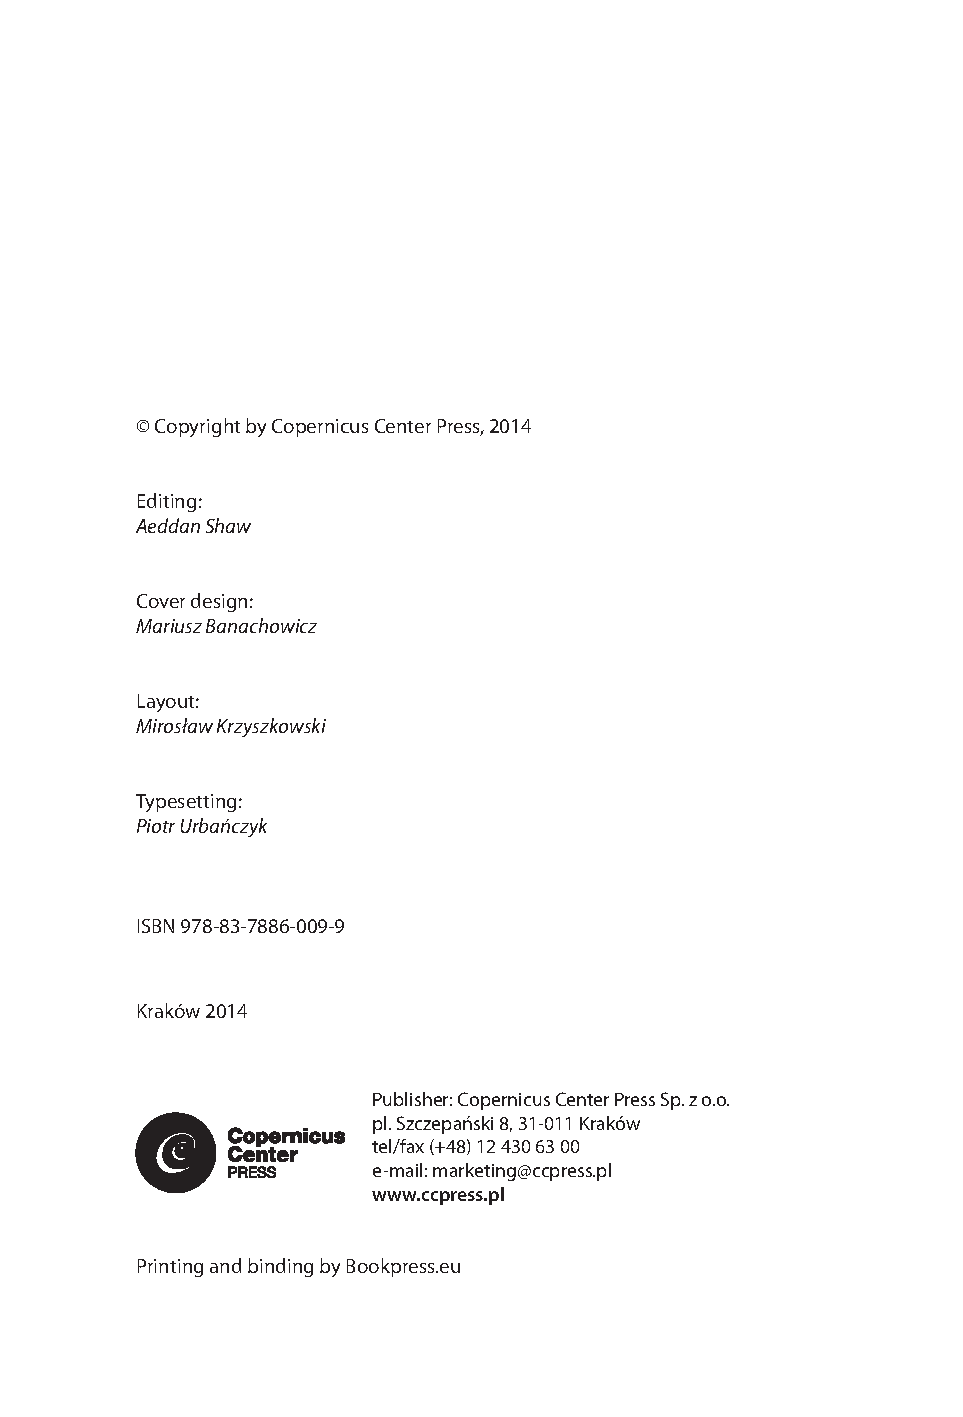
\includepdf[pages=1]{images/CT4.pdf}


\thispagestyle{empty}
\vspace*{1.2in}%
\begin{flushright}
\rectitle{Zagadnienia Filozoficzne\\w Nauce}\par
\vspace*{.5in}%
\chaptitleeng{Philosophical Problems\\in Science}\par
\end{flushright}
\vfill
\clearpage

\thispagestyle{empty}

\vfill

\noindent\begin{czw}© Copernicus Center Press, \rok\end{czw}

\vfill

\begin{adres}
	\begin{pagname}\noindent\begin{czwad}Editorial Board\end{czwad}\\
		Editor-in-Chief: dr hab. Paweł Jan Polak\\
		Deputy Editor-in-Chief: dr hab. Janusz Mączka\\
		Honorary Editor: prof. dr hab. Michał Heller\\
		Guest Editors: dr Bartłomiej Skowron, dr Michał Eckstein\\
		Editorial Secretary: Piotr Urbańczyk
		
	\end{pagname}
\end{adres}


\vfill


\noindent\begin{czw}Proofreading: dr Roman Krzanowski\end{czw}

\vskip.5em

\noindent\begin{czw}Adjustment and correction: Artur Figarski\end{czw}

\vskip.5em

\noindent\begin{czw}Cover design: Mariusz Banachowicz\end{czw}

\vskip.5em

\noindent\begin{czw}Technical editor: Artur Figarski\end{czw}

\vskip.5em

\noindent\begin{czw}Typographic design: Piotr Urbańczyk\end{czw}

\vskip.5em

\noindent\begin{czw}Typeset in \end{czw}\LaTeX

%\noindent\begin{czw}Skład: Artur Figarski\end{czw}


\vfill

\begin{adres}
	\begin{pagname}\noindent ISSN 0867-8286 (print format)\\
		e-ISSN 2451-0602 (electronic format)
	\end{pagname}
\end{adres}

\vfill

\begin{adres}
		\noindent\begin{czwad}Editorial Office\end{czwad}
	
		\noindent\begin{pagname}Zagadnienia Filozoficzne w Nauce
		
		\noindent Wydział Filozoficzny UPJPII
		
		\noindent ul. Kanonicza 9, 31-002 Kraków
		
		\noindent POLAND
		
		\vskip.3em
		
		\noindent e-mail: zagadnienia@upjp2.edu.pl
		
		\noindent www.zfn.edu.pl\end{pagname}
\end{adres}

\vfill

\begin{wrapfigure}{L}{.3\textwidth}
	\noindent\includegraphics[width=.29\textwidth]{images/ccp.pdf}
%\noindent\includegraphics[width=.27\textwidth]{images/ccp.pdf}
\end{wrapfigure}
\vskip.4em
%\noindent\parbox[t]{6cm}{
\begin{adres}
	\noindent\begin{pagname}Publisher: Copernicus Center Press Sp. z o.o.
		
		\noindent pl. Szczepański 8, 31-011 Kraków POLAND
		
		\noindent tel. (+48) 12 448 14 12
		
		\noindent e-mail: marketing@ccpress.pl
		
		\noindent www.ccpress.pl\\ \end{pagname}
	
	
\end{adres}
%}




\clearpage

%	\thispagestyle{empty}
	\begin{flushright}%
	{\bigtitle{Zagadinienia\\Filozoficzne\\w Nauce\par}}%
	\vspace{0.2in}%
	{\chaptitleeng{Philosophical Problems in Science\par}}%
	\vspace{0.2in}%
	\hrule%
	{\LARGE\textbf{{\numerrzymski -- \rok}}}%
	\hrule%
	\end{flushright}%
%		\@mkboth{\czwit\contentsname}{\czwit\contentsname}%
	\vspace{0.5in}%
%
%\clearpage

%Spis tresci -------------------------------------------------

{\thispagestyle{plain} \tableofcontents \clearpage}
%-------------------------------------------------------------
\newpage
\thispagestyle{plain}
\cleardoublepage
\thispagestyle{plain}

%-------------------------------------------------------------






%\ramkaart{Imię Nazwisko}
{Tytuł rozdziału.\\\chapsubtit{Podtytuł rozdziału}}
{Tytuł rozdziału. Podtytuł rozdziału}
{Tytuł rozdziału. Podtytuł rozdziału}

\lettrine[loversize=0.13,lines=2,lraise=0.00,nindent=0em,findent=0.2pt]%
{W}{}ielu filozofów i językoznawców twierdziło, że gdy identyfikujemy przedmioty, zarówno w języku, jak i w postrzeganiu, kierujemy się względami praktycznymi, potrzebami, wolą -- krótko mówiąc, swego rodzaju interesem, czy to gatunkowym (a więc ogólnoludzkim), czy to swoistym dla danej społeczności, cywilizacji czy jednostki. Wydaje się to kłócić z przeświadczeniem, że te przedmioty muszą istnieć, chyba że traktujemy to przeświadczenie jako jedną z wielu równouprawnionych wizji świata. Ta sama zasada wielości równosilnych perspektyw stosuje się a fortiori do języka metafizyki.

Tak więc powracamy tam, gdzie nasz horror bierze swój początek. Jakże mam trwać przy danym języku (czy jakimś szczególnym punkcie widzenia, z którego patrzę na świat, albo regule interpretacji całości doświadczenia), nie przyznając mu uprzywilejowanej poznawczej mocy? A jeśli pretenduję do dysponowania wyższym czy może nawet absolutnym językiem, to albo nadawałby się on tylko do mówienia o innych językach, nie zaś o rzeczywistości, do której się odnoszą, albo byłby standardowym językiem, a inne byłyby jego niekompletnymi dialektami. W tym drugim przypadku byłby to rzeczywiście boski język, absolutny i zawierający wszelkie wyobrażalne punkty widzenia. Lecz język taki jest niemożliwy; nawet Bóg, przemawiając ustami proroka, musiał się przełożyć na język ludzki; przekład jest niechybnie zniekształcony, a nam brak dostępu do oryginału. W przypadku pierwszym język mój (język pierwszego stopnia, język rzeczy) nie może wprawdzie rościć sobie pretensji do jakiejkolwiek pozycji uprzywilejowanej, lecz w tym języku nie sposób byłoby nieobecność owej pozycji wyrazić: by to uczynić, musiałbym swój język porzucić i przejść do super(czy meta-) języka -- ale w takim języku moje stanowisko, jako że szczególne, nie dałoby się wyrazić.

\myquote{
Gdy więc wielkodusznie powiadam: „wszystkie stanowiska metafizyczne są równie dobre”, sam żadnego stanowiska nie zajmuję, po prostu wyrażam zasadę tolerancji, która, jakkolwiek chwalebna, ma charakter formalny i nigdy nie wyda, czy choćby zainspiruje, żadnej metafizycznej idei. Lecz próbując zachować tę zasadę i obstawać zarazem przy swym szczególnym punkcie widzenia, popadam w niekonsekwencję, jako że twierdzę wtedy, iż „stanowisko moje jest tak samo dobre jak każde inne, mimo że jest nie do pogodzenia z żadnym innym”.

A jeśli tak mówię, nie mogę w zrozumiały sposób wyjaśnić, w jakim sensie to stanowisko jest moje, w przeciwieństwie do innych. Niestety, tolerancyjna wspaniałomyślność nie pozwala uciec od paradoksu samoodniesienia.
}

\noindent Leon Chwistek, logik i malarz, w wydanej w 1921 roku książce Wielość rzeczywistości sugerował istnienie czterech rodzajów wzajemnie niezależnych (a zatem przypuszczalnie nieinterferujących z sobą wzajem) rzeczywistości: rzeczy, takie jak je postrzega zdrowy rozsądek; rzeczy nauk fizycznych; wrażeń; i wyobraźni. Znajdują one swój artystyczny wyraz w malarstwie – odpowiednio: prymitywistycznym, naturalistycznym, impresjonistycznym, futurystycznym\footnote{To jest przypis dolny. Jeśli niezależne od siebie pokłady rzeczywistości wymagają dla swego opisu niezależnych języków, sugeruje to, że języki te są całkowicie nieprzekładalne; skoro tak, to w istocie można sądzić, że różne wizje świata współistnieć mogą w doskonałej wzajemnej obojętności}. Lecz wielość ta, dowodził, pozwala na dowolną liczbę równoprawnych poglądów na świat, z których żadnego nie można dowieść, lecz każdy jest do przyjęcia pod warunkiem, że nie próbuje zmonopolizować prawdy. Dopuszczalne stają się różne odpowiedzi na tradycyjne pytania, jak te o wolność woli, relację między ciałem a duchem, obiektywność wartości, jeśli zakres odniesienia ogranicza się do jednej lub niektórych spośród owych czterech rzeczywistości.

\noindent Leon Chwistek, logik i malarz, w wydanej w 1921 roku książce Wielość rzeczywistości sugerował istnienie czterech rodzajów wzajemnie niezależnych (a zatem przypuszczalnie
nieinterferujących z sobą wzajem) rzeczywistości: rzeczy, takie jak je postrzega zdrowy rozsądek

\section{Podtytuł 1 stopnia}

\noindent Teoria wielu -- jakkolwiek wyodrębnianych -- rzeczywistości, jeśli nawet w tym przypadku stworzona dla metafizycznej interpretacji malarstwa, proponuje przekonujący i kuszący obraz świata. Jednakże jako propozycja epistemologiczna nie jest w stanie -- czy to w wersji Chwistka, czy Williama Jamesa -- poradzić sobie z wciąż tą samą trudnością: jak dowieść wyższości pewnej teorii bytu w tym samym języku, w którym została wypowiedziana? Mieliżbyśmy utrzymywać, że twierdzenie „wszystko jest konieczne” jest równie prawomocne co twierdzenie „poza związkami logicznymi nic nie jest konieczne” i że doktryna, według której słowo „ja” nie ma odniesienia, jest nie mniej prawdziwa niż ta, wedle której cokolwiek ma odniesienie, jest względne w stosunku do „ja”?

\subsection{Podtytuł 2 stopnia}

\noindent Jeśli niezależne od siebie pokłady rzeczywistości wymagają dla swego opisu niezależnych języków, sugeruje to, że języki te są całkowicie nieprzekładalne; skoro tak, to w istocie można sądzić, że różne wizje świata współistnieć mogą w doskonałej wzajemnej obojętności: nie mogą być ze sobą konfrontowane ani między sobą sprzeczne. Ale twierdzenie, że nie mogą być konfrontowane, jest wyrażone w języku innym, wyższego stopnia, nie nadającym się do celów metafizycznych. I tu powraca ten sam kłopot: albo ograniczamy się do tego wyższego języka i wtedy werdykty nasze nie mają znaczenia dla rzeczywistych problemów, z których filozofia żyje, albo przyjmujemy pewną metafizyczną perspektywę i głosimy, że perspektywy tej, jako zamkniętej, nie da się zharmonizować z żadną inną ani też innej przeciwstawić -- i wtedy też, w wyniku tej samointerpretacji, perspektywa nasza jest bez znaczenia dla rzeczywistych problemów, z których filozofia żyje.

\sectionno{Podtytuł 1 stopnia}

\noindent Teoria wielu -- jakkolwiek wyodrębnianych -- rzeczywistości, jeśli nawet w tym przypadku stworzona dla metafizycznej interpretacji malarstwa, proponuje przekonujący i kuszący obraz świata. Jednakże jako propozycja epistemologiczna nie jest w stanie -- czy to w wersji Chwistka, czy Williama Jamesa -- poradzić sobie z wciąż tą samą trudnością: jak dowieść wyższości pewnej teorii bytu w tym samym języku, w którym została wypowiedziana? Mieliżbyśmy utrzymywać, że twierdzenie „wszystko jest konieczne” jest równie prawomocne co twierdzenie „poza związkami logicznymi nic nie jest konieczne” i że doktryna, według której słowo „ja” nie ma odniesienia, jest nie mniej prawdziwa niż ta, wedle której cokolwiek ma odniesienie, jest względne w stosunku do „ja”?

\subsection{Podtytuł 2 stopnia}

\noindent Jeśli niezależne od siebie pokłady rzeczywistości wymagają dla swego opisu niezależnych języków, sugeruje to, że języki te są całkowicie nieprzekładalne; skoro tak, to w istocie można sądzić, że różne wizje świata współistnieć mogą w doskonałej wzajemnej obojętności: nie mogą być ze sobą konfrontowane ani między sobą sprzeczne. Ale twierdzenie, że nie mogą być konfrontowane, jest wyrażone w języku innym, wyższego stopnia, nie nadającym się do celów metafizycznych. I tu powraca ten sam kłopot: albo ograniczamy się do tego wyższego języka i wtedy werdykty nasze nie mają znaczenia dla rzeczywistych problemów, z których filozofia żyje, albo przyjmujemy pewną metafizyczną perspektywę i głosimy, że perspektywy tej, jako zamkniętej, nie da się zharmonizować z żadną inną ani też innej przeciwstawić -- i wtedy też, w wyniku tej samointerpretacji, perspektywa nasza jest bez znaczenia dla rzeczywistych problemów, z których filozofia żyje.

\section{Podtytuł 1 stopnia}

\noindent Teoria wielu -- jakkolwiek wyodrębnianych -- rzeczywistości, jeśli nawet w tym przypadku stworzona dla metafizycznej interpretacji malarstwa, proponuje przekonujący i kuszący obraz świata. Jednakże jako propozycja epistemologiczna nie jest w stanie -- czy to w wersji Chwistka, czy Williama Jamesa -- poradzić sobie z wciąż tą samą trudnością: jak dowieść wyższości pewnej teorii bytu w tym samym języku, w którym została wypowiedziana? Mieliżbyśmy utrzymywać, że twierdzenie „wszystko jest konieczne” jest równie prawomocne co twierdzenie „poza związkami logicznymi nic nie jest konieczne” i że doktryna, według której słowo „ja” nie ma odniesienia, jest nie mniej prawdziwa niż ta, wedle której cokolwiek ma odniesienie, jest względne w stosunku do „ja”?

\subsection{Podtytuł 2 stopnia}

\noindent Jeśli niezależne od siebie pokłady rzeczywistości wymagają dla swego opisu niezależnych języków, sugeruje to, że języki te są całkowicie nieprzekładalne; skoro tak, to w istocie można sądzić, że różne wizje świata współistnieć mogą w doskonałej wzajemnej obojętności: nie mogą być ze sobą konfrontowane ani między sobą sprzeczne. Ale twierdzenie, że nie mogą być konfrontowane, jest wyrażone w języku innym, wyższego stopnia, nie nadającym się do celów metafizycznych. I tu powraca ten sam kłopot: albo ograniczamy się do tego wyższego języka i wtedy werdykty nasze nie mają znaczenia dla rzeczywistych problemów, z których filozofia żyje, albo przyjmujemy pewną metafizyczną perspektywę i głosimy, że perspektywy tej, jako zamkniętej, nie da się zharmonizować z żadną inną ani też innej przeciwstawić -- i wtedy też, w wyniku tej samointerpretacji, perspektywa nasza jest bez znaczenia dla rzeczywistych problemów, z których filozofia żyje.

\begin{thebibliography}{00}{Imię Nazwisko}
{Tytuł rozdziału. Podtytuł rozdziału}

\makeatletter
    \clubpenalty10000
    \@clubpenalty \clubpenalty
    \widowpenalty10000
\makeatother


\bibitem{Abc}
A.~Abc, \textit{Abc}...

\bibitem{Xyz}
A.~Abc, \textit{Abc}...

\end{thebibliography}





%\sekcja{Od Redakcji}{Editorial}

%\input{EDI/editorial-PU.tex}



\sekcja{Artykuły}{Articles}

%\renewcommand{\theequation}{\arabic{section}.\arabic{equation}}
%\input{ART_Majid/Majid.tex} 
%\renewcommand{\theequation}{\arabic{equation}}

\begin{artengenv}{Anna Sarosiek}
	{The role of biosemiosis and semiotic scaffolding in the processes of developing intelligent behaviour}
	{The role of biosemiosis and semiotic scaffolding in the processes\ldots}
	{The role of biosemiosis and semiotic scaffolding in the processes\\
	of developing intelligent behaviour}
	{Pontifical University of John Paul II in Krakow\label{sarosiek_anfang}}
	{Biosemiotics deals with the processes of signs in all dimensions of nature. Semiosis is the primary form of intelligence. Intelligent behaviour becomes immediately understandable in this approach because semiosis combines causality with the triadic structure of the semiotic sign. Intelligence is a~process created in a~given context. In the course of evolution organisms have learned to create increasingly sophisticated internal representations of external state. Semiosis is the precursor of the emergence of a~feature we consider intelligence. Biosemiotics also draws attention to the distributed intelligence, which relies on external semiotic scaffoldings as much as on the subject’s abilities and knowledge.}
	{biosemiotics, semiosis, biosemiosis, semiotic scaffolding, intelligence, cognitive activity, functional circles, Jakob von Uexküll.}





\section*{Introduction }
\lettrine[loversize=0.13,lines=2,lraise=-0.03,nindent=0em,findent=0.2pt]%
{B}{}iosemiotics is a~field of science connecting biology and semiotics. The primary purpose is to show that semiosis is an essential aspect of life. Biosemiotics aims to build a~bridge between biology, philosophy, linguistics and communication research. The main challenge of biosemiotics is to increase knowledge of biological information: recognition and interpretation of organic codes as the fundamental elements of the living world
%\label{ref:RNDdqbtpjMK0T}(Barbieri, 2005).
\parencite[][]{barbieri_life_2005}. %
 Thomas Sebeok applied biosemiotics to investigate the biological roots of human semiosis. He tried to understand the organic world as a~world of signals, signs, communication and language. Some biologists have begun to see how many phenomena and functions at the centre of organic life (genetic code, cell metabolism, ecosystem activities) are semiotic mechanisms 
%\label{ref:RNDhZlZ9AKzIY}(Anderson et al., 1984).
\parencite[][]{anderson_semiotic_1984}. %
 The signs and meanings play a~fundamental role in all activities of living systems. Semiosis is an indispensable feature of all life forms’ ability to accumulate, replicate, transmit and make sense of messages. The study of these communication processes and the meaning they produce can be considered a~life science discipline related to both nature and culture 
%\label{ref:RNDr7Hwb6LkCW}(Sebeok, 1991, p.22).
\parencite[][p.22]{sebeok_semiotic_1991}.%


Biosemiotics researchers accept the complexity of life processes as a~collection of data provided by biological sciences. Nevertheless, they consider also behavioural research. Biosemiotics deals with the transformation of signs in all dimensions studied, including the appearance of semiosis in nature, which can predict the features of living cells, the natural history of signs, aspects of semiosis in the ontogenesis of organisms, in plant and animal communication, and the functions of signs in immune and nervous systems as well as the semiotics of cognition and language
%\label{ref:RNDAID5Cb7So1}(Emmeche, 1992, p.78).
\parencite[][p.78]{emmeche_modeling_1992}. %
 Biosemiotics is perceived as a~contribution to the general theory of evolution, based on a~synthesis of various disciplines. The field proposes a~new approach to the phenomenon of life, considering the importance and the functions of a~single ribosome and ecosystem and the beginning of life and its meaning. The biosemiotic concept assumes the sphere of life is filled with sign processes, which result in the individual creation of meanings like food, the need to escape, and sexual reproduction. Jasper Hoffmeyer argues that semiotic requirements are a~condition for the success of species and that organic evolution is the evidence of the development of sophisticated semiotic means necessary for survival. The most visible feature of organic evolution is the plurality of morphological structures, as well as the development of ``semiotic freedom'', which means a~significant increase in ``richness or depth of meaning 
%\label{ref:RNDPentkhE2Nr}(Hoffmeyer, 1996, p.61).
\parencite[][p.61]{hoffmeyer_signs_1996}.%
''

In the research, the role of the observer of the system is equally important. One tries to understand the nature of observed phenomena to describe and conceptualize it. This position presupposes the possibility of conducting a~scientific experiment and observation and to measure various systems. These issues have been studied many times in the philosophy of science. Nevertheless, the research of living systems is developed by biologists and systems scientists
%\label{ref:RNDJUxAdYTWhF}(Kampis, 1991; Pattee, 1989, pp.63–78; Rosen, 1978; Uexküll, 1984).
\parencites[][]{kampis_self-modifying_1991}[][pp.63–78]{pattee_simulations_1989}[][]{rosen_fundamentals_1978}[][]{uexkull_semiotics_1984}. %
 The goal of biosemiotics is to identify assumptions, that are applied to the teleological concepts of biology: function, information, code, signal, cue and to provide them with a~theoretical grounding. Such terms in biology cannot be avoided or replaced by logical, chemical or mathematical concepts. Therefore, biosemiotics aims to consolidate these terms in the physical and biological context. It tries to define and relate them to evade the anthropomorphisms that are hidden assumptions of human science. Biosemiotics uses very carefully concepts that are regularly adopted to describe the evolutionarily complex product of semiotic processes as human culture. The efforts are made to avoid falsities of anthropocentrism or vitalism and distinguish which of these concepts are appropriate to the precise level of research 
%\label{ref:RNDHVKdE0q0Ey}(T?nnessen, 2013).
\parencite[][]{tonnessen_biosemiosis_2013}.%


The history of semiotics is deeply rooted in structuralism and linguistics. Biosemiotics is related to a~theoretical biology. Relations, meaning, wholeness and contextuality allow to perceive living creatures as active systems of sign production, sign mediation and sign interpretation. This approach explains the essence of behaviour and life filled by intentionality, self-awareness and sense, which are deeply connected with intelligence. Biosemiotics is the science of sign processes, which gives the instruments for scientific research and the study of these features.

The intelligence research is struggling with the problem of the lack of a~clear definition of the term ‘intelligence’. Consideration of intelligence is based on the properties of an organism that can be measured. Definitions of the term ‘intelligence’ are made by finding paradigmatic examples and creating lists of properties. These are characteristics that describe the properties and functions of living beings’ actions leading to effective action in the world. Intelligent behaviour is defined as adequate and effective behaviour leading to the achievement of a~specific goal. However, there is no equivalent definition, because the concept of intelligence is vague and inaccurate. Colloquial and scientific descriptions of intelligence are multiplying. However, in the current approach, it is defined as the ability to think, infer, make decisions, recognize patterns, predict the effects of one’s actions, the ability to remember, learn, problem-solving, perception, but also the ability to use language, motor skills, the use of intuition, being creative and conscious, i.e. general coping with the world
%\label{ref:RNDBPtBfYkfR3}(Rosen, 1978).
\parencite[][]{rosen_fundamentals_1978}. %
 This work tries to justify the concept of intelligence in a~biosemiotic context, which is broader than human
%\label{ref:RND4UZRqvH0L3}(Byrne, 2004; Goldstein, Princiotta and Naglieri, 2014; Pfeifer and Bongard, 2006; Spearman, 1904; Thorndike, 2017)
\parencites[][]{byrne_2004}[][]{goldstein_2015}[][]{pfeifer_2006}[][]{spearman_1904}[][]{thorndike_animal_2017} %
 or artificial intelligence AI 
%\label{ref:RNDpjVwUVRBFp}(Brooks, 1986; Kurzweil et al., 1990).
\parencites[][]{brooks_1986}[][]{kurzweil_1990}. %
 %Brooks, 1986; Huw, n.d.; Kurzweil et al., 1990
Thus, the concept of ‘intelligence’ will be presented as a~result of semiosis.

\section*{The conceptual problem of intelligence}
The ways of describing intelligence are changing over time. The common search for characteristic properties and specific determinants tries to justify intelligent behaviour. Arthur Jensen, one of the leading psychologists studying human intelligence, hypothesized that all human beings share the same intellectual mechanisms, and that differences in intelligence are related to ``quantitative biochemical and physiological conditions
%\label{ref:RNDjbalXtcVjE}(Jensen, 1998).
\parencite[][]{hoffmeyer_unfolding_1998}.%
'' He meant skills such as attention, perception, generalization, learning, memory, language, thinking, and problem-solving. In addressing the subject of the intelligent behaviour of living organisms, we do indeed reflect on the mechanisms underlying such action. First, the properties that seem to be crucial for the phenomenon of intelligence are distinguished. It is not considered as a~whole of behaviour but attempts to isolate those features that seem important and decisive for intelligent action.

Intelligence as the body’s ability to react in complex ways to environmental stimuli (as in biosemiotics) is closely related to the ability to think. It is a~Cartesian legacy of Western culture. For Descartes, there were two separate substances: physical and mental
%\label{ref:RND3PSZmfafdq}(Descartes, 1637).
\parencite[][]{descartes_discours_1637}. %
 This division gave rise to the historical problem of how mutual relations between the two systems---body and mind---can proceed since each of them can exist without the other. One of the main challenges posed by this dilemma is how a~thought, or something that happens in an immaterial mind, can affect the material body. To this day, the problem of substantial dualism is considered in modern science as a~mind-body problem. Descartes also argued that the bodies of animals and humans are simple mechanisms because they are subjected to external factors and act by mechanical forces 
%\label{ref:RNDnLqvAmGGx2}(Descartes, 1641).
\parencite[][]{descartes_renati_1641}. %
 The premise of Cartesian dualism is that the material body has certain physical properties and their description is provided by mathematical natural science. Only the ability to think, which belongs only to man, allows for rational and conscious management of one's own body. Self-awareness, on the other hand, is the result of a~way of understanding oneself through causality or logic and a~condition of cognition. This view made the human mind perceived as a~peculiar value and all other beings are measured by its measure.

Most people would probably agree that mental phenomena such as thinking come from processes in the brain and that there is the mind that controls these kinds of actions. However, the description of mental activity presents some fundamental problems. So far, this type of mind operation has not been comprehensively described. While we all have a~fairly clear idea of the term ‘thinking,’ it remains poorly defined. Thinking is understood as the possibility of inducing, inferring, looking for analogies, performing calculations and recognizing patterns, largely coincides with intelligent behaviour in the description.

Deep Blue met the requirements described above and performed the expected actions, but it is still not called intelligent
%\label{ref:RND5FmPuOtJgo}(Deep Blue, 2012).
\parencite[][]{noauthor_deep_2012}. %
 Similarly, other programs that mimic the human cognitive mechanisms also do not get the term ‘intelligent’. Interesting examples are expert systems that discover patterns and find the best possible solutions. However, a~diagnostic program will not be considered smarter than the average doctor, even if its knowledge base is larger, it works is faster and its diagnoses are more accurate. The ability to solve problems is always placed high among the characteristics of intelligent organisms. It is related to the previously acquired knowledge and the possibility of its creative use. Programs recognize emotions, chatbots build complex and grammatically correct sentences. Some programs create images and music. Moreover, the capabilities of artificial systems, especially those related to computational capabilities, often far exceed human skills.

The early AI research methods were based on the consideration of high-level symbolic representations. The ability of logical reasoning, i.e., 
the ability to play chess,
solving mathematical problems or deduction, was considered to be  the manifestations of intelligence. Research on artificial intelligence was based on colloquial or psychological understanding. Colloquially, intelligence is usually considered to be the ability to solve practical problems, language skills or social competencies. In psychology, it was most often considered an efficiency that determines the effectiveness of actions, using cognitive processes, which is controlled by the superior ability of the mind, corresponding to the mental level of the individual and special abilities, responsible for the efficiency of action in specific areas or types of tasks. The research program has always been based on the current knowledge and beliefs about the phenomenon of intelligence.

\section*{The fundamental importance of semiosis}
Semiosis distinguishes living systems from inanimate ones
%\label{ref:RND7hry0nIuRm}(Sebeok, 1988b).
\parencite[][]{sebeok_communication_1988}. %
 Friedrich Rothschild argues that ``living systems formed from the very beginning as signs systems 
%\label{ref:RNDbsTmIxbWoQ}(Rothschild, 1962).
\parencite[][]{rothschild_laws_1962}.%
'' The significant and necessary premise of biosemiotics is the appearance of meaningful communication in species other than \textit{Homo sapiens}. Semiosis is the process of creating, receiving, and interpreting characters. Any form of activity, behaviour or process that involves signs is an aspect of semiosis. Semiosis is a~process that produces and carries meaning. It also mediates the relationship of purposefulness and causality, because it allows to search and connect hidden meaning.

The idea of semiosis was originally developed to relate language to other sign systems, both human and non-human. Moreover, the prototype of semiotic theories is language. Processes of semiosis can be applied to other sign systems (but then sign systems already presuppose semiosis)
%\label{ref:RNDxsCcfmjwwC}(Noth, 2002).
\parencite[][]{noth_semiotic_2002}. %
 Some hypotheses describe meta signal systems and interpret language as one of the various codes for communicating meaning. Such a~perspective is predefining semiosis as an act of the communication of meaning established within the relationship of signs 
%\label{ref:RNDoqfKrONq0d}(Bateson, 1966; Pavlov, 1927).
\parencites[][]{bateson_information_1966}[][]{pavlov_conditioned_1927}.%


Semiosis is a~broad phenomenon concerning social interaction systems and its significant aspect of information exchange. Greater or lesser extent semiotic exists in nature as the linguistic message, ways of thinking, emotional reactions, beliefs, motives and goals. In semiosis the processing of information associated with the emergence of meaning and causality is equally important. In the biological context, systems that transmit, acquire, assimilate, decode and manipulate information, is generating a~meaning. The emergence of information implies thinking. Obtaining information begins a~cause-and-effect process. It is the causative factor that ensures that one event is linked to another in a~chain of thought
%\label{ref:RND432gOW9NnM}(Pharoah, 2020).
\parencite[][]{pharoah_2020}.%


All the aspects of semiosis described above are related to the conditions for the emergence of intelligent behaviour. Emotional states, feelings and beliefs encoded in the message are transmitted the same way as the essential information about objects and situations. The transformation of signs develops dynamically in the process of communication. The reception, interpretation and production is neither chaotic nor random. The answer is more than a~stimulus or a~simple response. Among the many possibilities of interpreting the sign, the body chooses the optimal one for itself. Signals are transmitted to evoke a~specific reaction in the process of semiosis, which requires a~proper attitude to the received signals.

Observations of the behaviour of living organisms show that the simplest forms of life use a~system of signs. It is especially apparent among animals that inform other members of the herd where they found food, announce the time of fertility to other individuals of the same species, and warn themselves of threats. Messages take various forms: chemical, audible, visual or tactile transmitted as individual signals or a~complex of them
%\label{ref:RND6q7iEGUfQD}(Sebeok, 1969).
\parencite[][]{sebeok_semiotics_1969}. %
 Sebeok suggests that endosymbiosis, self-reference, receptor functions, autopoiesis, and other living system properties align with the definition of semiosis: something is alive and communicates meaning 
%\label{ref:RNDQD071qwpmb}(Sebeok, 1988a, p.72).
\parencite[][p.72]{sebeok_animal_1988}. %
 It does not convey discrete information but gives it a~deeper meaning. The emergence of meaning is the beginning of intelligent behaviour, because it evokes suitable actions in the particular context of environment.

The course of the semiosis process also requires evaluation. Organisms receive enormous amounts of sensory data from the environment as well as from their interior. Totally number of signs processes will not run at the same level due to the possibility of sensory overload. The brain cannot handle all the information simultaneously. Therefore, there must be a~classification of the signs in terms of their meaning (for example, related to experience or current need). The signs become operational when distinguished from background noise. Cognitive activity is triggered to interpret the input data and transform it into meaningful information. Kalevi Kull
%\label{ref:RNDgLADMGwMiW}(1998)
\parencite*[][]{kull_semiosis_1998} %
 argues that there is a~repetitive order of semiosis:

\begin{enumerate}
\item the cognitive entity filters environmental data and recognizes signs (based on a~pre-existing model in memory);
\item meaning arises in mind---as a~new structure, but the explicit isomorphism is visible within the original and the new sign;
\item the sign is interpreted as meaningful and matched with existing patterns and their meanings stored in memory;
\item the results of a~successful interpretation are an observable response to perceived stimuli.
\end{enumerate}
Thus, in the beginning, a~recognition process takes place. It begins the semiosis process and is necessary at other levels. The arising meaning is not only recalled from memory but re-created and compared with previous experiences. The intelligent reaction requires the suitable selection of the appropriate interpretation of the sign but can differ significantly from the existing ones.

The subject transforms signs and retains the result of the interpretation---the physical development and the way the memory works are the results of previous semiosis processes. In this perspective, intelligent action appears as a~continuous interpretation of meaning influenced by its historical circumstances. According to Yuri Lotman
%\label{ref:RNDGOxZNS0qW6}(1990, p.101),
\parencite*[][p.101]{lotman_universe_1990}, %
 ``the sign itself is a~program for the creative process.'' Each sign interpreted by the mind has already been interpreted and stored in the memory, and the result of the interpretation influences the process by passing it on as a~sign to subsequent recipients. The components of semiosis are continuously interpreted. It becomes possible to create new and forget old meanings. The creativity of mind can produce new relationships and some strength of ``rewriting'' meaning over pre-existing engrams. The emergence of meaning is the creative work of the organism. During semiosis, relationships arise between things that do not interact or influence each other through direct physical or chemical processes. Such semiotic phenomena do not belong to the physical, but the mental. They are evidence of the intelligent relationship to reality.

All forms of cognition emerge from the interpretation of signs. It is a~result of the structural coupling of the subject and its environment. Those relations must proceed to guarantee the integrity and durability of the organism’s world. The living system structures and the environment are changing as a~result of their interaction. The coupling that arises from their plasticity produces an autonomous and well-defined unit. The relation develops the history of the subject. Cognition is associated with an embodiment, embedding and situated experience because it always includes a~subject defined by physical and mental architecture
%\label{ref:RNDl9bdWwwtAg}(Wilson and Golonka, 2013; Lakoff and Johnson, 2008; Miles, Nind and Macrae, 2010).
\parencites[][]{wilson_embodied_2013}[][]{lakoff_metaphors_2008}[][]{miles_moving_2010}. %
 Cognition immersed in the world defines dynamics events taking place in specific contexts in space and time. Such an individual is capable of learning from experience and adapting his behaviour accordingly. Semiosis allows overcoming the dualism of mind and body by observing the transformations of signs. This approach provides a~better understanding of living systems than the dichotomies of mental and physical properties made by other natural sciences. Semiosis is a~dynamic process, and it can potentially last indefinitely.

Semiosis is a~process, which prefers signs that are meaningful for organisms. During semiosis, intelligent behaviour is an experienced application of functions as transmission and creation of new information. Not entirely predictable data, which not comply with existing patterns, get the ability to preserve and selectively recreate the knowledge. Intelligence does not appear as a~fuzzy concept, but as a~developed ability to use signs and properly use environmental signals and organize knowledge.

\section*{Biosemiosis theory of Jakob von Uexküll}
One of the pioneers of behavioural physiology, ethology and the precursor of biocybernetics, was Jakob von Uexküll (1864-1944). He devoted his work to the research of perception and actions of living creatures. Uexküll has introduced the term \textit{Umwelt} to describe the subjective world of the organism
%\label{ref:RND6WWnDIrGBs}(Uexküll, 1921).
\parencite[][]{uexkull_umwelt_1921}. %
 He developed a~distinctive method he called \textit{Umweltforschung}. The scientific goal of Uexküll was to investigate the behaviour of organisms as subjects in families and groups. Uexküll theory of signs and meaning has the place in all aspects of life processes. The concept of the functional circle (\textit{Funktionskreis}) is the interpretation of the general model of sign process---semiosis. A~description of the functional circle allows understanding how intelligence arises in operations of the living system.

Uexküll strongly emphasized the essential role of the physical architecture of the organism in shaping forms of interaction with the outside world. He tried to create a~new idea based on theoretical foundations. The new conception provided to organize the research and understand how living organisms function in the world
%\label{ref:RNDRParn16QgX}(Uexküll, 1920, p.7).
\parencite[][p.7]{uexkull_theoretische_1920}. %
 Uexküll’s research perspective was different due to the dedication of a~principle recognizing reality as a~``subjective insight'' of a~specific organism 
%\label{ref:RNDAaQkEoF4wd}(Uexküll, 1920, p.9).
\parencite[][p.9]{uexkull_theoretische_1920}. %
 In this way, he interpreted Immanuel Kant’s views presenting objects as phenomena that owe their structure to the subject 
%\label{ref:RNDcoXyfSBOEl}(Uexküll, 1920, p.8).
\parencite[][p.8]{uexkull_theoretische_1920}. %
 The biologist argued that the role of the sensory organs and the central nervous have an enormous role in the Umwelt construction. Another goal would be to examine the relationship of animals with the experienced objects of the world. Uexküll was interested in studying the subjective reality of animals. He argued that different species with different sensory feelings experience the world differently.

The physical nature of specific sensory apparatus influences a~particular world view
%\label{ref:RNDvGDzstF58Q}(Uexküll, 1934, p.22).
\parencite[][p.22]{uexkull_streifzuge_1934}. %
 Uexküll believed that one could access different Umwelts via the study of the physical organization of organisms. According to him, this access required immersion in the anatomical structure of the examined organism, which is responsible for the way it interacts with the outside world. Cognition is a~subjective process that takes place in a~species-specific area. The semiotic processes are responsible for the dynamics of cognition by linking the subject with the contextual world. There is a~particular symbolic sphere that contains a~range of possible interactions according to the mode of interaction permitted by the physical architecture of the organisms’ forms. The type of perception also shapes the environment---Umwelt---the significant world.\footnote{German term ‘\textit{Umwelt}’ refers to the environment or surroundings. However, the term used by Uexküll is an interpretation of reality and distinguish from the environment---\textit{Umgebung}. The Umwelt of organisms is the projection of the world created inside them by the same. Umwelt is a~world experienced by an individual organism.} In this Umwelt, specific environmental features become essential and individualized. Furthermore, these peculiarities are perceiving as qualitatively distinct and assigned particular meanings. In this belief about the subjectivity of the experienced world, Uexküll was supported by Ernst Cassirer which argued that all living beings have their circle of action, which is both a~limitation and a~point of view a~specific world 
%\label{ref:RND7tBkh94GJj}(Cassirer, 1996).
\parencite[][]{cassirer_philosophy_1996}.%


Natural systems are pre-equipped with genetic information that guides the organism through different life cycles in different environmental contexts. The genetic data is a~kind of embodied pre-empirical knowledge and inherited memory that allows the system to identify and assign meaning to specific environmental signals and produce the appropriate behaviour as a~response to meet the demands of its \textit{Innenwelt}
%\label{ref:RNDe5nDlXoMyK}(Uexküll, 1921, p.46).
\parencite[][p.46]{uexkull_umwelt_1921}. %
 The concept of Innenwelt refers to the inner world and contrasts with Umwelt pointing to an experience coming from within the body. Umwelt is a~particular world view. Innenwelt is defined by internal states which characterize the physical state of an individual. The Innenwelt concept seems to be systemic. It is essential to explain why particular environmental features have greater importance than others.

Uexküll's theory makes one wonder how the world reality is described and what it means to be an animal. Not only does it multiply worlds in a~variety of environments, but it also tries to reject the understanding of the animal as a~soulless machine, a~mindless or impassive object. One can recognize here the biological interpretation of Kant. Uexküll states that the world owes its existence to the organism’s internal subjective organization, which turns sensory features into a~spatial form
%\label{ref:RNDPNpI1bWCXU}(Uexküll, 1920, p.12).
\parencite[][p.12]{uexkull_theoretische_1920}. %
 Uexküll had also introduced a~new way of thinking about reality as more than just the physical world. He was one of the first biologists which emphasize the subjective experience of an animal.

One sees the development of an animals’ intelligence in observing its behaviour in its environment. Uexküll postulated to treats animals as subjects and as entities whose primary activity is perceiving and acting. Everything that the subject perceives becomes its world of perception (\textit{Merkwelt})
%\label{ref:RND3G0utXH9GM}(Uexküll, 1934, pp.26–28).
\parencite[][pp.26–28]{uexkull_streifzuge_1934}. %
 Everything the subject does becomes its world of action (\textit{Wirkwelt}). Uexküll focused on the subjective environment of animal and its relationships which may not be noticed by the human-researcher. An animal in its environment deals with many objects with which it can interact. Some of the perceived things become carriers of meaning when they enter into a~relationship with the subject 
%\label{ref:RNDe2roScZjZy}(Uexküll, 1934, pp.105–107)
\parencite[][pp.105–107]{uexkull_streifzuge_1934}.%
\footnote{Uexküll shows an example of a~stone-throwing at a~barking dog. The stone as a~physical object does not change, yet there is a~major change in its meaning. As long as it lay on the road, it not grab the dog's attention. It turns into a~carrier of meaning as soon as it enters into a~relationship with the dog/subject. Now, the stone becomes a~bullet associated with a~feeling of pain. The subject produces meaning. This example shows the importance and primacy of functional relations.} Objects are experienced because of their functional meanings to the subject. The study of perception cannot be isolated from other bodily functions. It should be regarded as a~phase of action related to motor and intellectual activity. Living organisms exhibit activity as long as some meaning to them derives from functional relationships with other objects, whether they are spatial, temporal, causal, or purposeful relationships.

To adequately explain theory, Uexküll presented a~concept of the functional circle. This concept is an influential conceptual tool that emphasizes the subject’s interaction with the environment. It offers an instrument to describe the sensorimotor activity. In the perspective of Uexküll’s research behaviours are not movements or tropisms as Jacques Loeb would have wished
%\label{ref:RND6t2Nh8l6mh}(Loeb, 1907, pp.151–156)
\parencite[][pp.151–156]{loeb_concerning_1907}%
\footnote{Jacques Loeb developed a~theory of animal behaviour based on tropism---involuntary, forced movement. He presented the animals’ response to a~stimulus as a~direct and automatic response. He believed that the behavioural response was forced by the stimulus and does not require an explanation in terms of the animal’s supposed consciousness.}, but consist of perception (\textit{Merken}) and action (\textit{Wirken}). Behaviour is not the result of mechanically regulated reflexes but it is organized according to the subject's body composition and sensory abilities 
%\label{ref:RNDsH9ZTqXBQZ}(Uexküll, 1982, p.26).
\parencite[][p.26]{uexkull_theory_1982}. %
 The functional circle describes the basic structure of the interaction between animal and objects appear in the Umwelt 
%\label{ref:RNDhV05hT2tOT}(Uexküll, 1934, p.27).
\parencite[][p.27]{uexkull_streifzuge_1934}. %
 Subject capture the neutral object from the environment as a~meaning carrier and a~perceiving organ or a~perceiving cell, modify it by an effector organ and use it to respond 
%\label{ref:RND4BoP1il7b7}(Uexküll, 1987, p.170).
\parencite[][p.170]{uexkull_sign_1987}. %
 Each organism simultaneously observes the world and changes it. The functional circle shows how the organism interacts as a~subject with the object of its action.

In every process in which the organism is involved, the carrier of meaning plays a~leading role, either as a~carrier of a~perceptual stimulus or as a~carrier of an effector stimulus
%\label{ref:RNDVUxL8A9wWu}(Uexküll, 1982).
\parencite[][]{uexkull_theory_1982}. %
 According to Uexküll, the functional circle transforms sensory data into meaning. The circle processes trigger the subject’s reaction. Meaning here is understood as a~structure that connects perception and action. Functional circles present the act of biosemiosis, which is the basis for the formation of cognitive processes. One can see how the organism and its environment feedback enables rational action in Umwelt. Object and subject in a~circle connect and form a~whole. An individual is formed through the plasticity of the semantic structure and experience. The subject can identify signs and gives meaning to specific environmental cues. It produces behaviour that the external observer perceives as adequate and intelligent, and for the organism conforms to its own needs and requirements 
%\label{ref:RNDXM7JxXuRx6}(Uexküll, 1934, pp.28–29).
\parencite[][pp.28–29]{uexkull_streifzuge_1934}.%


The subject uses his sensorimotor system to meet its needs effectively. Features of the subject are structurally related. Features with perceptual meaning affect features of an operational nature and vice versa. The subject’s state changes causing it to adapt to the environment and situation in the best possible way. One observes an action that bears the signs of intelligence. Even a~simple organism uses the sensory organs and the motor organs to process meaning to the best effect.

Depicting an animal’s senses and motor organs as these were machine parts ignores their actual functions and operation. The sensations and the acting will, are a~kind of perception of the operator built into these organs. Everything subject perceives results in the subjective perception of the world. The operator acts according to its own needs which form a~closed whole which is its Umwelt. A~simple functional cycle presents receptors and effectors signals as the manifestations of the subject’s actions. Objects are merely carriers of meaning. The observation of animals behaviour leads to the conclusion that they act intelligently. No matter how simple the symptoms are. One cannot describe intelligence in terms of one-sided human definition because intelligence is a~result of subjective perception and action.

The functional circle model contains all elements that are part of the meaning process. The connection of them depicts the process of semiosis. The subject interprets the external signals as the sign; the sign evokes the biological state of the organism; the biological state determines behaviour. On the other hand, there could be an object that is hard to interpret. Any object may have a temporary
existence as a different semiotic object i.e., the meaning of anything may change. The functional circle connects perception and action that enables the understanding of reason and goal of the action. Objects can be associated with the other items through different functional circles. The more complicated organism has a~greater number of circles. Nevertheless, the organism deals with perception and action to imprint its meaning on the meaningless object and makes it a~carrier of meaning for the subject in Umwelt
%\label{ref:RND8x8dSdW7Pd}(Uexküll, 1934, p.110).
\parencite[][p.110]{uexkull_streifzuge_1934}.%


Umwelt of an animal is only a~fragment of the universe that the human observer perceives as the human world. One needs to recognize the perceptual signals of all stimuli in the environment to consider the intelligent operation of the system. That is the first condition to understand the Umwelt of the organism in which certain objects and situations become the reason for taking actions. The organism can perform the number of functions which is equal to the number of objects. This number increases if the number of objects that fill the Umwelt increases too. Each new experience is associated with re-adaptation to new situations. Uexküll noticed that objects of cognition are transformed into perceptual signals and become real objects of Umwelt
%\label{ref:RNDbwAgtViSpi}(Uexküll, 1934).
\parencite[][]{uexkull_streifzuge_1934}. %
 Things do not gain value until they are transformed into the carrier of meaning. A thing without a~relationship remains meaningless. The meaning depends on the perception of the object and the action dependent on the need. From Uexküll's point of view, the properties of an object are a~perception marked as meaningful by the subject in a~relationship with it. Objects are initially neutral in the subject's universe. Objects become carriers of meanings by giving them a~function which depends on the mood and needs of the subject.

Animals like humans exhibit activities that are attempting to exceed biological constraints. Uexküll was aware that perception and action also depend on the experiences of the cognitive subject. New experiences give rise to generalizations that become the point for creating new levels of generality. The process of learning, adopting new patterns, looking for alternative explications can start again on a~new level. Jesper Hoffmeyer calls a~network of interactions that span living systems semethic interaction. Semethic interaction is the habit acquired by an individual, which is used (and interpreted) by others of the same species so it induces new habits in the particular group
%\label{ref:RNDGExh7UPE60}(Hoffmeyer, 1998).
\parencite[][]{hoffmeyer_unfolding_1998}. %
 That means that any regularity developed in a~living system (on any level) tends to create new interpretations and build a~set of new experiences.

The concept of the formation of meaning presented by Uexküll makes it possible to use biosemiotics to study intelligence. Biosemiotics is placing interpretation at the centre of attention. It shows that semiosis is an inevitable feature of life and argues that the process of meaning is a~fundamental form of intelligence. Uexküll proved that the concepts of biosemiotics, although started from the attributes of objects (their perception and actions) cannot depend on specific physical implementation. According to Peirce, semiotic communication includes the sign, the object of the sign, and the interpreter
%\label{ref:RNDfClkaMysma}(Peirce, 1998).
\parencite[][]{peirce_essential_1998}. %
 Anything must be understood to be a~sign. The signs require interpretation, otherwise, they may not even be considered signs. The basic principle of Peirce’s semiotics is that index and iconic signs have no meaning in isolation 
%\label{ref:RNDWErWIt9enB}(Peirce, 1998).
\parencite[][]{peirce_essential_1998}. %
 Biosemiotics takes these issues seriously. It tries to present an approach to the idea of shaping mental states and the biological sources of this process as well. According to Uexküll's theory one cannot ignore semiotic interactions at any level. To capture the meaning, one has to perceive signification, representation and reference as distinctive on any occasion.

\section*{Embodiment and intelligence}
The body is an essential factor enabling cognition or thinking. The existence of the body is a~necessary condition for intelligence. Especially the embodiment of mental processes is a~leading topic in cognitive science and neurobiology
%\label{ref:RNDhO80G68YtS}(Clark, 1997; Damasio, 1994; Deely, 1990; Lakoff and Johnson, 1999; Varela, 1993).
\parencites[][]{clark_being_1997}[][]{damasio_descartes_1994}[][]{deely_basics_1990}[][]{lakoff_philosophy_1999}[][]{varela_embodied_1993}. %
 The body’s sensors deliver sensory signals to the brain and provide a~basis for action. For example: grasping small objects with your fingertips is simple because there are more sensors than in the finger joints or the metacarpus. The grasp of a~small hard object requires more limited control due to the deformable tissue of the finger. Some elements of the neural control are taken over by the morphological and material properties of the hand. The material properties of the musculoskeletal system allow making quick movements. Even then, the nervous system is too slow to control all details of the movement 
%\label{ref:RNDBbqi11VBD0}(Clark, 1997; Damasio, 1994; Deely, 1990; Lakoff and Johnson, 1999; Varela, 1993).
\parencites[][]{clark_being_1997}[][]{damasio_descartes_1994}[][]{deely_basics_1990}[][]{lakoff_philosophy_1999}[][]{varela_embodied_1993}. %
 One of the aspects of the brain works is proprioception---awareness of body mobility and position. Even most simple moves require constant feedback from the proprioceptive organs in the body. Proprioceptive organs measure muscle strain and cell layer displacement including the gravitational orientation. Maxine Sheets-Johnstone suggests that the proprioceptive sense is a~bodily awareness. Any self-moving creature feels his movement and his stillness 
%\label{ref:RND2oq6ptThjc}(Sheets-Johnstone, 1998).
\parencite[][]{sheets-johnstone_consciousness_1998}.%


Cognitive science assumes that concept formation is related to specific motor programs motivated by perception and action in an experimental context. Eleanor Rosch proves that the basic concepts in the human mind are related to types of things or actions with which subject has motor experience
%\label{ref:RND6uJBCE7W1t}(Rosch, 1999).
\parencite[][]{rosch_principles_1999}. %
 Afterwards, one can create schematic representations of images: tables, walls, bicycles, buildings, talking, walking, sleeping, etc. Sensory-motor knowledge of the world determines the fundamental concepts of the world. The primary concepts have a~core, depending on the basic functions of the organism. The large part of them is related to the perception and practice of acting in a~settled environment. Embodied gestures become mental patterns used in perception and reason (part-whole, centre-periphery, goal-path, straight-curved and near-far, cycle, contiguity, movement, balance). The structures of these gestures are body goal-oriented. As the consequence elementary bodily experiences are the starting point for mental activities. The result of experiencing states and things in the world arises as an abstract thought. George Lakoff and Mark Johnson constructed a~groundbreaking theory. They model a~bodily metaphor as a~relevant cognitive tool providing structural metaphors led on metaphorical expressions.\footnote{For example, the structured conceptual metaphor ``Knowledge is seeing'' experience in many continuous languages a~series of different expressions such as ``enlightenment'', ``Can’t you see what I~am explaining?'', ``Look at the problem'' 
%\label{ref:RNDMZkc53iwuI}(Lakoff and Johnson, 2008).
\parencite[][]{lakoff_metaphors_2008}.%
} Imagination turned out to be the substantial instrument using metaphors and building developed conceptual models in thought experiments: idealized cognitive models constructed from basic concepts, schemas and mappings between them.

Biosemioticians study the embodied nature of the mental realm. The statement that mental processes are embodied implies their natural history of formation and development. One cannot separate it from embodied life. Mental life grounds at bodily intentionality manifested in the cycles of perception-action, thus ultimately in biosemiosis. Neurosciences reveal numerous mechanisms that may explain the effects of the sensory system in behavioural development
%\label{ref:RNDhClIGKtAiP}(Purves, 1988, pp.19–20).
\parencite[][pp.19–20]{purves_body_1988}. %
 There is a~relationship between body structure and the central nervous system. The number of mechanisms: muscle trophic responses, processes caused by the activity of sensory and motor cells, and hormonal changes influence distant parts of the body. Informational signals are generated in the various sensory channels through the physical interaction of the living system with the environment. The feeling of moving is caused by seeing changes in the environment that correlate with a~muscle strain. Objects closer appear to move faster than those farther away. Consequently, the body is informed about the distance. There is a~relationship between the brain’s neural activity, body morphology (shape and material properties) and interaction with the environment used to achieve specific tasks. Various cellular processes lead to the survival of the relevant neurons and different forms of the nervous system.

Merleau-Ponty identified primal awareness as not ``I think'' but ``I can''
%\label{ref:RNDvuftmKLf11}(Merleau-Ponty, 2001, p.156).
\parencite[][p.156]{merleau-ponty_fenomenologia_2001}. %
 The initiation of a~movement coexists with the motivation to perform it and requires the species-specific mobility range. It is the base of the ``I can'' potential, which subordinates the proprioceptive states and possibilities of the subject’s action. The body---carrier of meaning---allows feeling the external features of the environment, sensations of movement and stimulus from the inside. The potential possibilities of the body turn ``I can'' into ``I do''. Merleau-Ponty points out that the behaviour of an organism in Umwelt is more primary than awareness, which is only one of the particular forms of this behaviour 
%\label{ref:RNDk80o8RLt0v}(Merleau-Ponty, 2001, p.239,393).
\parencite[][p.239,393]{merleau-ponty_fenomenologia_2001}. %
 The connection between the body and the environment is the fundamental condition for the emergence of conscious functioning. Feeling and movement (perception and action) enable the body to discover and understand Umwelt. The sense organs in the functional circles make possible the body to act more precisely. It means that the animal distinguishes its spatial position due to an inherent neural proprioception system that facilitates feedback control of behaviour in relation to the proper perceptual and behavioural worlds. The perceptual world becomes comprehended because the body perceives itself. The represented world of the mind is the clue of possibility and choice to act intelligently in it.

Merleau-Ponty’s interpretation of Edmund Husserl’s concept is interesting. Husserl’s problem, as Merleau-Ponty argues, is to find a~place for nature in the philosophy of reflection
%\label{ref:RNDYpoLAKtCa7}(Merleau-Ponty, 2003, p.72).
\parencite[][p.72]{merleau-ponty_nature_2003}. %
 The perception of nature allows for the correlation of the environment and consciousness in \textit{Lebenswelt}. Merleau-Ponty portrays Husserl’s ``body-world'' as an Umwelt sensory engine. He explains a~way of perceiving as the motor capabilities of the subject’s body: the function of the body 
%\label{ref:RNDUnbZXhWv4i}(Merleau-Ponty, 2003, p.74).
\parencite[][p.74]{merleau-ponty_nature_2003}. %
 The body is suited for being in the world. The world becomes a~part of the subject’s body. It guarantees the possibility of orientation, not only in space-time but in all normative scales. Merleau-Ponty’s phenomenological interpretation of Uexküll’s theory shows the Umwelt as the actuality of existence. Behaviour in such Umwelt cannot be understood with the moment, but only as a~significant whole of existence in time. Symbols affect the animal in current orientation, respond to options and lead to future perception.

\section*{Fundamental role of semiotic scaffolding}
The Uexküll functional circle is the blueprint of the sensory-motor body. The body is conceived as a~semiotic device perceiving and acting in its surroundings through signs
%\label{ref:RND1UnYgD9VWX}(Heidegger, 1992, p.261).
\parencite[][p.261]{heidegger_grundbegriffe_1992}. %
 Uexküll admitted the existence of indefinite neutral objects in Umwelt which are necessary to increase the complexity of the Umwelt 
%\label{ref:RNDSnj3ixXzlm}(Uexküll, 1934, pp.92–93).
\parencite[][pp.92–93]{uexkull_streifzuge_1934}. %
 The perception of neutral objects is a~prerequisite condition for learning. Placing them in the action of existing functional circles makes it necessary to expand circles. The adaptability of circles presupposes the perception of neutral objects that are initially irrelevant but cause an imbalance in the alignment of the organism to the environment. The development of the functional circle is triggered by increasing semiotic complexity. The situation of growing environmental pressure results in the optimal tension in the previously defined functional circle by adjusting it to the occurring changes.

Due to the organism’s autonomic activity, some actions accomplish well when information is incomplete. An autonomously functioning system can fill knowledge gaps by using external data. It is possible by the network of semiotic interactions with which individual cells, organisms or populations control their actions
%\label{ref:RNDe6tQGQ86jH}(Kull, 2015).
\parencite[][]{kull_evolution_2015}. %
 Semiotic scaffolding provides organisms with precise actions by ensuring efficient interaction with key signs arising in dynamic situations (e.g. hunting or mating). This term is understood in a~general sense as an entity or process that supports another process and thus enhances the stability, functioning or range of possibilities of cognitive activity 
%\label{ref:RND1ecHE08Vtt}(Emmeche, Kull and Stjernfelt, 2002, p.29).
\parencite[][p.29]{emmeche_reading_2002}. %
 Patterns of action emerge as intelligent system behaviour of various autonomous activities depends on the environment. Semiotic scaffolding takes the place of a~centralized decision-making system based on internally represented directions of activities or goals. Horst Hendriks-Jansen stated that interactive behaviour could be explained in generative terms because there are not internal rules to predict the types of behaviour that occur.\footnote{The concept of generativity describes an autonomous system that creates and uses new unique behaviours without relying on external data of this system 
%\label{ref:RNDxptcDXaTqv}(Hendriks-Jansen, 1996, p.9).
\parencite[][p.9]{hendriks-jansen_catching_1996}.%
} Andy Clark 
%\label{ref:RNDBGUO37p9LU}(1997, p.46),
\parencite*[][p.46]{clark_being_1997},%
 on the other hand, suggested that intelligent creatures use environmental structures for their purpose instead of storing or expensively processing information.

The importance of scaffolding has already been emphasized by Lev Vygotsky, who described the child’s development as gaining experience with the support of external structures.\footnote{It can be physical support when learning to walk or swim, or language support when learning to speak
%\label{ref:RNDoTFfYGAY0m}(Vygotsky, 1964).
\parencite[][]{vygotsky_thought_1964}.%
} New skills can be socially transferred from caregiver to child through mimicry or scaffolding when a~more capable adult manipulates the pupil’s interactions with the environment to develop novel skills. Scaffolding reduces the distance, highlight the most considerable characteristics of the task, decrease the number of steps in the performed plan and allow the finish the action. Scaffolding is necessary to experience before the child gains an independent cognitive or physical ability to seek and achieve a~goal. The concept of scaffolding describes living organisms use external structures to simplify tasks. Natural language and information technology are an example of a~powerful semiotic human scaffold. Human knowledge can be written in books and passed on. Man can rely on what was already established and written down: ideas in one text rely (directly or indirectly) on other texts. The World Wide Web with text, pictures, sound and video made the web of knowledge and ideas clearer and more accessible 
%\label{ref:RNDIWQyrnwJiZ}(Clark, 2004).
\parencite[][]{clark_natural-born_2004}.%


Scaffolding is raised to make a~building but limits and determines the way a~skyscraper is built. The semiotic control of biological actions also limits and determines the time and manner in which activity takes place. Conceptualization and analysis of semiotic scaffold mechanisms operating at different natural systems levels are the core of biosemiotics research. Semiotic scaffolding obtains many forms, but their primary property remains the focus of an organism’s behaviour on a~limited repertoire of possibilities or guiding behaviour to implement a~sequence of actions. The cell receptor is tuned to open when and only it hits the appropriate stimulus, e.g. an amphibian’s eye is the result of formed chemical interactions between the newly formed optical vesicle and the embryonic layer of the ectoderm. The chemical inductor produced by the optical vesicle is used as the scaffold for this action
%\label{ref:RNDmInECjoP0B}(Kull, 2014).
\parencite[][]{kull_catalysis_2014}. %
 This example shows the important aspect of development as the ability of individual cells to alter their internal settings under the influence of external factors or new molecular cues.

Scaffold-based activities become more complicated as the life cycle of organisms becomes complex or subject begin to engage in social processes. Semiotic mechanisms depend on changes in interpretations that always assume error. They also rest on the ability to foresee and prepare for the events and life cycle incidents. Gene scaffoldings work by controlling and assembling proteins converted into patterns that reflect the organism’s needs
%\label{ref:RNDA6AUvdDFj2}(Hoffmeyer, 2014).
\parencite[][]{hoffmeyer_semiome_2014}. %
 These mechanisms work well as long as the behavioural repertoire is limited to instinctively triggered responses to predictable events. However, animals with large brains, such as birds or mammals, depend on learning processes in addition to their instinctive reflexes. Such processes are genetically assisted by the provided preferences, but the ability to learn must be an integral part of behavioural flexibility. The transfer of behavioural control from the genome level to the brain level introduces the need to use scaffolding mechanisms.

Organisms use scaffolds to refer to the environment, to symbolize, to reason, to use patterns. The benefits from the abilities are acquired through phylogenesis or ontogenesis to establish regularities in the environment and direct actions accordingly. A~Ringed Plover, which pretends to have a~broken wing to distract a~weasel from its nest takes advantage of the predator’s semiotic scaffolding to be fooled by false signs. The bird deceives the mammal because it has genetically or ontogenetically acquired knowledge of how the predator will interpret the apparent relationship. However, there may be times when a~weasel is not deceived, so it proves that its responses are not strictly deterministic. The predator may or may not misinterpret the sign. It also means that the sign essence is the relational nature of causing awareness of something that is not in itself. This fact implies a~full Peircean sign triad that can arise in any system capable of autonomous anticipatory activity.

Semiotic scaffoldings are related to the interaction of the body’s interior and surroundings. They occur in the semiosphere of living organisms, which rely on communication with the world around them by sounds, smells, movement, colour, shape, electric field, chemical signals, touch and provide them with cognitive activity. The semiosphere is the result and condition for culture development by analogy with the Vladimir Wiernadski’s term ``biosphere''. Semiosphere is an organic whole of living nature and also a~place for the continuation of life
%\label{ref:RNDBTZNG5SfoG}(Lotman, 1990, pp.12–126).
\parencite[][pp.12–126]{lotman_universe_1990}.%
\footnote{Lotman, who introduced the concept ``semiosphere'' used it as an analogy with the term ``biosphere'' by Vladimir Wiernadski. Although in Lotman’s writings, semiosphere is associated formerly with culture, he presents semiosis as the fundamental mechanism of action that connects the entire semiotic space. The concept of Wiernadski's biosphere did not survived in this sense. Now, it is a~term ``ecosystem'' including the earth with the inhibited organisms.} The concept of semiotic scaffolding of the semiosphere gives a~semiotic dimension to life processes emphasizing their belonging to the world of sign activity. Uexküll presented the processes of building independent relations with the world as a~necessary condition for the autonomously functioning system.

Species have limited access to this semiosphere because they can interpret potential signals in its environment. They evolved to fit into a~specific ecological niche. This niche contains all information and directions that must be correctly interpreted by the organism. The number of features of the world becomes mattering indications of an organism’s behaviour. It is infinite and more than the number of traits with which the organism interacts physically. The bird must notice the possibility of food or shelter to obtain the best effect but use semiotic scaffolds that are patterns of sounds, directions and wind speed, differences in air or temperature, changes in the intensity and wavelength of light. There are many environmental changes during the animal’s life. Therefore, the semiosphere and semiotic scaffolding indicate an enormous amount of possibilities for action or adaptation. Organisms cannot react only passively or instinctively to states and events. Instead, they perceive, interpret and act in the environment in a~way that creatively and unpredictably alters all evolutionary and selective settings.

Intelligence is a~sophisticated activity traditionally seen as extending the biological behaviour of animals. Modern research, however, recognizes that animals possess intelligence
%\label{ref:RNDrkME9KRdd5}(Waal, 2016; Heinrich, 1999; Fischer and Menzel, 2011).
\parencites[][]{waal_are_2016}[][]{heinrich_mind_1999}[][]{fischer_animal_2011}. %
 Many biologists have long believed that instincts and intelligent behaviour are in opposition to each other. They argued that successful action is a~coincidence of instincts interaction 
%\label{ref:RND2TjEYo9od4}(Richter, 1927; Thorndike, 2017, p.150).
\parencites[][]{richter_animal_1927}[][p.150]{thorndike_animal_2017}. %
 It is worth emphasizing, that intelligence is not the elusive trait somewhere in mind, but is related to social abilities, the ability to use physical signs, and the ability to accumulate and organize knowledge. Peirce defined the term ``semiotic'' as characteristic for all signs used by an intelligence capable of learning through experience 
%\label{ref:RNDNFUp52vkZ1}(Peirce, 1994 par. 227).
\parencite[][]{peirce_collected_1994}. %
 Extending intelligence to all living systems is an attempt to bridge the ontological gap between humans and animals. It also allows you to look at machine intelligence without having to refer to the human cognitive system.

Semiosis plays a~central role in experiencing and gaining knowledge about the world. The semiotic process penetrates the beginning, middle and end of the development of every organism. In the semiotic system, plans and concepts without intelligent actions would not take place. Therefore, symbolization is the basis of intelligence. Biology and semiotics are intertwining more and more. Biology provides solid empirical support for the understanding that semiotic faculties are the essence of intelligence. Each biological or genetic code is a~semiotic system par excellence and can be interpreted as the basis of intelligence itself: the connection of the genetic codes contained in living cells with the very nature of these cells, the differentiation and integration of these cells into complex organisms, their development in various organs, and ultimately organization in the brain. Intelligence indicates the process of experiencing the physical world that makes sense for structures and the whole life of the organism.

\section*{Conclusion}
Animals exhibit intelligent behaviour, such as planning, hunting for a~particular type of prey, remembering to find or build a~shelter, participating in courtship, and using other strategies commonly thought to occur only in higher species. For Uexküll, it was related to the natural cycle of life, based on the principles regulating life activities. In the subjective Umwelt, the animals produce variants of actions, perceive gradations, anticipate failures and they are deceived by illusions. The animal perceives the world in an integrated way without breaking it down into parts, colours or sounds. Its perceptions and actions are intelligent, context-sensitive and deeply meaningful. Experiencing a~specific situation is determined by changing moods, current needs and intentions and sensory-motor skills. Skills develop through the world experience, practice and therefore appear to play a~pivotal role in the embodiment and situating of intelligent behaviour
%\label{ref:RNDEJ1KZ3QtFR}(Dreyfus, 1979; Searle, 1992).
\parencites[][]{dreyfus_what_1979}[][]{searle_rediscovery_1992}.%


Earlier attempts to deal with this knowledge resulted in the theory of mind-body dualism. The biosemiotic approach can help since perceive meaning (\textit{sema}) as inherent to the body (\textit{soma}). The body is involved in communication processes that coordinate the activity of cells, tissues and organs. The exchange of messages integrates the different levels of the hierarchy. In this standing, intelligence is the interface of the organism manages its relationship with the surrounding environment. Organisms are systems that cannot be interpreted as being independent of the environment but as adaptive systems.

Mental life is grounded in bodily intentionality manifested as the cycles of perception and action. This activity integrates organisms’ survival strategies. Above all, it is a~deliberate action---a~precursor of life dimension. At higher animals is perceived as intelligence and ultimately consciousness. Biosemiotics explores the fundamental processes of mental life arising and argues that the whole organism functions are semiotic processes that precede the emergence of authentic intelligence. The semiotic scaffolding ensures that appropriate cognitive level is obtained and improves the cognitive functions of the subject. Distributed cognition describes cognitive acts as the result of the system operation. It involves the subject, others and objects and the situational context in the environment. Distributed intelligence involves support to perform an action that would otherwise be error-prone, difficult or impossible to achieve. The activities based on external scaffolding can enable understanding of intelligent behaviour that is supported outside the mind. By the analogy of embodied and situated artificial agents to some animals this perspective could be useful for understanding of artificial agents’ intelligent behaviour.

\end{artengenv}
\label{sarosiek_ende}

\begin{artengenv}{Radosław Kycia}
	{Information and brain}
	{Information and brain}
	{Information and brain}
	{Masaryk Univeristy, Department of Mathematics and Statistics\\
	Cracow University of Technology, Faculty of Materials Engineering and Physics\label{kycia_anfang}}
	{We present the consequences of the assumption of the classical and quantum nature of information storing and processing in the brain. These assumptions result in different behaviours of consciousness under a hypothetical brain copy experiment. The subject is important in the context of 'mind uploading' considerations.}
	{classical information, quantum information, brain models, mind uploading.}
	
	


%%%%%%%%%%%%%%%%%%%%%%%%%%%%%%%%%%%%%%%%%%%%%%%%%%%%%%%%%%%%%%%%%%%%%%%%%%%%
%Introduction
%%%%%%%%%%%%%%%%%%%%%%%%%%%%%%%%%%%%%%%%%%%%%%%%%%%%%%%%%%%%%%%%%%%%%%%%%%%%
\section{Introduction}
%%%%%%%%%%%%%%%%%%%%%%%%%%%%%%%%%%%%%%%%%%%%%%%%%%%%%%%%%%%%%%%%%%%%%%%%%%%%
The brain is the most complicated organ in the human body and it is still not well understood. It is responsible for `high-level' capabilities such as reasoning and intelligence. Recently, greater efforts have been made to understand the structure and its exact working principles through the Brain Research through Advancing Innovative Neurotechnologies (BRAIN) project, announced by the United States Government in 2013 \parencite{BRAINInitiative}. This project mainly focuses on the structural approach to the brain and on collecting data on the neuronal activities within it.

Currently, there exist exact simulations of the brain parts up to the level of cells, e.g. the Blue Brain Project \parencite{BlueBrainProject}. There are also mathematical models of some of its regions, e.g. the hierarchical temporal memory (HTM) of the neurocortex \parencite{CortexModel1, CortexModel2} which is based on hidden Bayesian networks \parencite{KurzweilHowToCreateBrain}. These ideas have been used successfully in software for speech and image recognition. There are also interesting connections of models of the visual cortex with differential geometric structures \parencite{VisualCortex}, describing structures above the level of single neurons and their interconnections.

At the level of single cells, there are various models of neurons and their interactions used in computational neuroscience, see e.g. \parencite{ModellingNeurons} and references therein. In short, neurons communicate with other neurons, exchanging electric impulses (modifying ion density locally within the cell or using chemical neurotransmitters at synapses, the interface between neurons). The neuron has some threshold of activation above which it 'fires' producing a spike in voltage. In models based on neurons, memory and learning ability of the brain result from a `plasticity' of neuron synapses---change of neurons interaction intensities encode new and modify existing data in the brain. In this approach, the topology of the neural network as well as the properties of single neurons are taken into account. These models use non-linear differential equations, stochastic models, and/or a control theory approach.

However, there is no unifying idea of precisely how the brain works and how elements/parts induce high-level capabilities. There is not even any consensus regarding whether the brain operates on classical principles alone, or whether quantum principles need to be included as well. Recently, there are reports on the importance of quantum mechanical processes in neurons  \parencite{EmperorsNewMind, PenroseQuantum1, PenroseQuantum2}. Furthermore, a new discipline of quantum biology \parencite{QuantumBilogy} has been established: the discipline of biology that examines the relevance of quantum level processes (tunneling, entanglement) in living organisms. We want to strongly stress that the current state of knowledge indicates that quantum processes are not essential on scales larger than chemical compounds \parencite{QuantumBilogy}. In our presentation, we do not exclude these as they provide an effective comparison between the classical and quantum approaches to brain functionality. New results suggest that the quantum processes as entanglement is possible also in hight temperatures \parencite{HightTempEntantgelemnt}. The other reason is that we do not know with precision the basic principles according to which the brain as a whole operates, even if the entirely classical paradigm currently appears most probable.


It is currently impossible to describe the brain structure strictly and there are many gaps in the present state of knowledge of brain operating principles. Therefore, in this article we reduce all complex problems to maximally simple and general ones. We consider the possible implications of the assumption that the brain works solely on classical principles and compare it with the quantum level approach. This enables us to define transcendental properties (i.e. if the properties of the brain configuration can be copied beyond the body). We elaborate this by considering a 
\textit{Gedankenexperiment} of brain copy to a virtual model. At the current level of technology and our understanding of the brain it is impossible to make. Such kinds of thought experiments provide a framework for understanding some aspects of consciousness from different angles \parencite{MindUploading2, KurzweilHowToCreateBrain}. This experiment fits into contemporary philosophical considerations regarding mind uploading \parencite{Transhumanizm, MindUploading, MindUploading2}. The other aim is to continue the discussion from \parencite{EmperorsNewMind} on the implications of the assumptions as to the principles according to which the brain operates.

The paper is organized as follows. In the next section, a review of the basic facts and properties of classical and quantum representation of information is provided. The section thereafter contains a formulation of the thought experiments on copying brain functionality to a machine. This allows us to deduce how assumptions regarding quantum or classical information in the brain will result in the possibility of copying the brain and therefore on the uniqueness of `consciousness'. The final section presents our conclusions.



%%%%%%%%%%%%%%%%%%%%%%%%%%%%%%%%%%%%%%%%%%%%%%%%%%%%%%%%%%%%%%%%%%%%%%%%%%%%
\section{Classical and quantum information properties}
%%%%%%%%%%%%%%%%%%%%%%%%%%%%%%%%%%%%%%%%%%%%%%%%%%%%%%%%%%%%%%%%%%%%%%%%%%%%
In this section, we focus on the properties of classical and quantum representation of information and their computation, which will prove useful in the next section.



%%%%%%%%
\subsection{2.1. Classical representation of information}
%%%%%%%%
We start to outline the information theory. It is a large subject including many branches \parencite{RezaInformation}. Here we focus on the basic properties that will be useful in subsequent sections.

Information describes results of our interaction with some object---a source of information. We consider a binary source that can produce two types of experimental outputs when we interact with it by recording answers for questions, e.g., about shape, colour or other information about the object. This set of questions and answers constitutes one way in which we encode our interactions with the world. We can associate these two outputs with letters (usually called `bits' in this context) from the alphabet $A=\{0,1\}$. Therefore, the output of the experiment is a sequence of letters, e.g. a word of length $N$ is an element of $A^N=A\times \ldots \times A$, where $\times$ indicates the Cartesian product. In computer science, the sequence of eight bits constitutes a byte. In binary computers, bits are stored in a physical structure called a `register' that is constructed from cells that are sequentially organized and can store one of two values from $A$. 

The numbers (integer, real, complex, etc.) can be coded into letters of $A$. This procedure starts by associating elements $A$ as representation of numbers of base\footnote{$\#A$ means the number of elements of the set $A$.} $N=\#A$, where letters from $A$ are associated (with some assumed order) to digits $\{0,1,\ldots, N\}$. Then the coding of a real number is a set (possibly infinite) of answers for questions if some number in the decoding procedure is larger than $lN^{n}$, where $n$ is an integer number and $l$ is a number associated with a letter of alphabet. For instance, for binary system $A=\{0,1\}$ we have  $5 = 1\cdot2^{0}+0\cdot 2^{1} + 1\cdot 2^{2} = 101_{2}$, that is, $2^{2} < 5 <2^{3}$ and $ 2^{0} \leq 5-2^{2} < 2^{1}$, which is process of discretization/quatization. There is also an interesting question to be raised about the efficiency of the coding of numbers. The most efficient choice of base is for the base of natural logarithm  $N=e$, see e.g., \parencites{kycia_information_2020}{KyciaNiemczynowicz} and references therein.

Moreover, for an analog signal that is described by a function $f:\mathbb{R}\rightarrow \mathbb{R}$, we can quantize and sample it in specific time intervals. This gives us a discrete representation of the signal. The bound on information loss during this process in the simplest case is controlled by the standard Nyquist--Shannon sampling theorem for equidistant sampling \parencite{Probing, RezaInformation} or by more elaborated sampling theorems.

All the above considerations reinforce the statement that we can restrict ourselves to  $A=\{0,1\}$ as each piece of information can be reduced with arbitrary accuracy to the sequence from $A$, providing a suitable coding method. These data can be processed digitally.

There also exists an approach to information in a statistical sense developed by Shannon \parencite{RezaInformation}. It focuses on analysis statistical properties of subsequences of bits in information. This statistical approach focuses on the efficiency of coding and not on the information itself, because a string of `bits of information' is treated statistically. Therefore, we will not deal with this notion in this paper. We do not care here about the efficiency of coding, as we will try to reduce the problem to fundamental principles, not necessarily efficient ones.


Later, we will be using the copy machine defined by the following operation:
\begin{equation}
\begin{array}{c}
 c: A^N \times A^N \rightarrow A^{2N}, \\
 c(M,a)= [M,M],
\end{array}
\end{equation}
where $a$ is an arbitrary sequence of $N$ bits, and the result is repeated two times the pattern of bits $M \in A^N$. After copying, the linear projection on the second component can be performed to isolate the copied data. Such duplication can be derived from the diagonal morphism  \parencite[see][]{RosettaStone_Baez} $\Delta :A \rightarrow A \times A$ that acts as $\Delta (x) = (x,x)$ for some $x \in A$.

The most important observation is that the copy operation can be conducted without perturbing the physical memory. This results from the statement that classical measurements can be designed not to perturb a memory based on the classical laws of physics. This is aside from the notion of information and is instead a statement on classical physics itself as well as the representation of information in systems obeying classical laws. We will see below that this changes when information is stored in quantum systems: this will be the core of our further considerations.


Information stored in classical system will be called classical information for short. In the next subsection, a review of quantum information properties is presented.

%%%%%%%%
\subsection{2.2. Quantum representation of information}
%%%%%%%%

The natural framework for quantum information/computing is a Hilbert space, i.e. data are represented as vectors of a complex inner product vector space, which is also a complete topological space \parencite{FunctionalAnalysisReed}. In the standard approach, a finite-dimensional vector space is used with a base of dimension $N >0$.

A single quantity of information is stored as a (complex) linear combination of base vectors. Depending on the dimensionality of the base, it is called a `qubit' for $N=2$ and a~`qudit' for $N>2$ \parencite[see e.g.][]{QuantumComputing}. We will focus here on qubits because, for qudits, the description is analogous. The dimension of the space determines the number of elements in the vector base and is called the `degree of freedom' of the qudit. For a qubit, the normalized vector describes a point on a sphere $S^{2}$ called the Bloch sphere \parencite{QuantumComputing}. This point on this sphere can be represented as a set of coordinates and even decoded to, for instance, the binary form described previously. Therefore, we can code classical information in qubits and vice versa. As we will see, the difference is in the physical properties of the quantum carrier of information. 

For quantum states the Hilbert space of the compound system is the tensor product of its constituents, in contrast to the Cartesian product for classical information. Therefore, if $\mathcal{H}$ is a Hilbert space for a single qubit then a register of $r>0$ such qubits is realized as a device that can store elements from
\begin{equation}
 \bigotimes_{k=1}^{r} \mathcal{H}.
\end{equation}

The square of the inner product of two qubits has the interpretation of the probability of finding the state of the system described by the first qubit in the state of the system described by the second qubit. Therefore, its value belongs to the unit interval $[0; 1]$ for all times. This imposes substantial requirements on the type of allowable operations realizing computations on quantum registers, namely they have to be unitary operations, that is, surjective isometries of the inner product.

There are two fundamental `no-go' properties that characterize quantum in formation and that will be used in the following section. They characterize a quantum representation rather than information itself. The first is the no-cloning theorem, which in its elementary version was originally published in \parencite{NoCloning_WootersZurek}. The formulation uses the unitary 'copying machine'/cloning operator $U$ which copy states as follows\footnote{The notation $|\psi>$ for a vector in the Hilbert space $\mathcal{H}$ was invented by Paul Adrien Maurice Dirac and is called 'bra-ket' notation \parencite{QuantumComputing}.}
\begin{equation}
 \begin{array}{c}
  U: \mathcal{H} \otimes \mathcal{H} \rightarrow \mathcal{H}\otimes \mathcal{H}, \\
  U( | \psi> \otimes |a >) = | \psi> \otimes |\psi >,
 \end{array}
\end{equation}
where $|a>$ is an arbitrary (non-zero) vector in $\mathcal{H}$ onto which copy is made. The no-cloning theorem of Wootters and \.{Z}urek reads
\begin{Theorem}
\label{Th.NoClonning}
 If $dim\mathcal{H}>1$ then no cloning machine exists.
\end{Theorem}

The proof is simple\footnote{
We provide the proof from \parencite{NoCloning_WootersZurek} for interested readers since it illustrates the idea of tensor product of quantum states/qubits.

 The proof relies on linearity of $U$ and of tensor product. From cloning property of $U$ we obtain:
 \begin{equation}
 \begin{array}{c}
  U\left( \frac{1}{\sqrt{2}}(|1>+|2>)\otimes|1>\right)  =  \frac{1}{2}(|1>+|2>)\otimes(|1>+|2>) \\ 
  =\frac{1}{2}(|1>\otimes|1>+|1>\otimes|2>+|2>\otimes|1>+|2>\otimes|2>),
 \end{array}
 \end{equation}
and from linearity we get
\begin{equation}
\begin{array}{c}
 U\left( \frac{1}{\sqrt{2}}(|1>+|2>)\otimes|1>\right)  = \frac{1}{\sqrt{2}} U(|1>\otimes |1>) + \frac{1}{\sqrt{2}} U(|2>\otimes |1>)  \\ 
  =\frac{1}{\sqrt{2}}(|1>\otimes|1>+|2>\otimes|2>).
\end{array}
\end{equation}
Since these two computations are not equal, so it contradicts the assumption that $U$ exists.
} and relies on incompatibility of linear operator $U$ and tensor product.


The intuitive notion of this theorem is as follows: if unknown quantum information is written on a quantum carrier, it cannot be copied in a quantum (unitary) way, that is, without interacting with information.

The no-cloning theorem has serious implications of both theoretical and practical importance  \parencite{QuantumComputing}. The restriction $dim\mathcal{H}>1$ for large quantum systems is automatically fulfilled. The tensor product used for describing composite quantum systems (and therefore quantum registers) is restrictive when only unitary operators are allowed. On the contrary, the Cartesian product used for classical information leads to no such constraints. Note also that the state to be copied is unknown at the beginning: if it is known, then we can produce a copy without affecting the original state.

The second important theorem in quantum computing is the no-deleting theorem, or indestructibility of a quantum state \parencite{NoDeleting_PatiBraunstein}, namely
\begin{Theorem}
\label{Th.NoDeleting}
 For an unknown state $|\psi> \in \mathcal{H}$ there is no linear isometrics operator $D$ acting as $|\psi>\otimes |\psi> \otimes |\psi_{env}> \rightarrow |\psi>\otimes |0> \otimes|\psi_{env}'>$ with the last state in the result: $|\psi_{env}'>$ that is independent of initial state $|\psi>$. If such deletion operator exists, then the state $|\psi>$ can be restored from the state of the environment $|\psi_{env}'>$, that is the environment state after deletion in such situation will depend on deleted state $|\psi>$.
\end{Theorem}
For generalizations see \parencite{NoDeleting_PatiBraunstein2}. There is however a quantum deleting operation that contains measurement of a state $|\psi>$, i.e., when in the process of deletion the state is revealed/known.

Note that for deletion of $|\psi>\otimes |\psi_{env}>$ if the final state $|0>\otimes |\psi_{env}'>$ would be $|\psi_{env}'>$ that is, independent of the initial state, then it would violate the uniqueness of unitary evolution in quantum mechanics. In essence, any initial data can end with the same final state during evolution, leading to a contradiction. 

The validity of Theorem \ref{Th.NoDeleting} is again a reflection of the presence of the tensor product in composed quantum state/register.


We also comment here on classical-quantum physics correspondence. At the most fundamental level, the laws of classical physics are derivable from quantum laws. However, when the quantum effects are negligible, then we can use classical laws with reasonable accuracy. In this regime, the effects of the influence of a measured object by a measuring device can be neglected. This is the origin of the distinction between quantum and classical information carriers.


%%%%%%%%%%%%%%%%%%%%
\subsection{2.3. Computation}
%%%%%%%%%%%%%%%%%%%%
The theory of computation and computational complexity is also a large subject on its own \parencite{HopcroftUllman}. Therefore, we will restrict ourselves to an overview of how we can reduce the problem of computation to a theory of a Turing machine or a Lambda calculus \parencite{LambdaCalculus, RosettaStone_Baez, HopcroftUllman}.

The process of computation can be associated with solving problems, and models of computation with an algorithm. A Turing machine model offers a conceptual framework for a computation process, divided into:
\begin{itemize}
 \item {A 'hardware' part---realizes computation as a mechanical device;}
 \item {A 'software' part---contains a programme that drives the process of computation;}
\end{itemize}
Every computation process equivalent to a Turing machine can also be decomposed into these two functional parts. We will use this remark below.

A Turing machine $M$ specialized to solve some class of problems can be treated as an input for the universal Turing machine $U$, which in some sense emulates $M$ producing the same output on initial data $x$ as $M$ does. In strict terms, $U(M;x) =M(x)$. Therefore, universal Turing machine can be seen as a simulation device for some specialized machines treated as algorithms. 

There are the different realizations of computations. As mentioned above, a Turing machine is a mechanical model of computation, whereas a Lambda calculus represents the functional approach to computation. However, by commonly accepted hypothesis---the Turing-Church hypothesis/conjecture \parencite{HopcroftUllman}---the Lambda calculus model is equivalent to the universal Turing machine. This means that if a given problem is computable by one computation model, then it is computable by the second one. The equivalence of models is proved by showing that one model can simulate the other model and vice versa. Moreover, a Turing machine (and therefore a Lambda calculus), although constituting a simple (abstract) mechanical machine, can be used to simulate the work of real computers \parencite{HopcroftUllman}. This may be a not optimal simulation, but it is possible. 


From the quantum perspective, there are a few models of quantum computations \parencite{QuantumComputing}, e.g., quantum gates, adiabatic quantum computers or topological quantum computers. However, they are all equivalent and we can focus on one of them, specifically the quantum gates approach, whereby quantum gates representing unitary operators are applied to the quantum bits described above. In this approach, quantum computation is reduced to linear algebra in a suitable Hilbert space. This is a problem that can be simulated by classical computers and therefore modelled by a Turing machine or an equivalent model. However, for a particular class of problems, quantum computing may outperform, in time complexity of computations, the classical approach \parencite{QuantumComputing}.  

Summing up, at the level of computing, the classical and quantum approaches are comparable, hence we reduce the problem to the universal Turing machine. The real distinction is at the level of the representation of data by a classical or quantum carrier. This determines if we can copy unknown data from the system without affecting it.


In the following section we present our attempt to apply the above facts regarding classical and quantum information properties to the transcendental properties of the brain. From the next section, speculative considerations start.



%%%%%%%%%%%%%%%%%%%%%%%%%%%%%%%%%%%%%%%%%%%%%%%%%%%%%%%%%%%%%%%%%%%%%%%%%%%%
\section{Brain copy}
%%%%%%%%%%%%%%%%%%%%%%%%%%%%%%%%%%%%%%%%%%%%%%%%%%%%%%%%%%%%%%%%%%%%%%%%%%%%
This section examines the implications of the assumption that the brain is a computational engine that operates on a programme and data that are encoded in a classical or quantum carrier.


The consideration here touches the notion of consciousness. For the needs of this section, we define this term as the complete functionality of the human brain, including the aspects that make us aware of our existence. If we reasonably assume that all our thinking is localized in the brain and the neural system, then this is the only place with which consciousness may be associated. By considering only the human brain, we reject all questions about the level of evolution of animals at which consciousness, in the sense of self-awareness, emerges. For humans, this notion is contained in the full functionality of the human brain.

Moreover, the definition above encapsulates what `consciousness' is currently believed to be. Indeed, this term brings together the currently poorly known principles constituting the brain functions \parencite[see, e.g.][]{Transhumanizm}. We will, however, comment on the more metaphysical term 'soul' in the next section.

We will not comment on the history of the term `consciousness' in philosophy, as there is already rich literature on this subject, including an overview in  \parencite{StanfordEncyclopedyOfPhilosophy_Conciousness} with an extensive bibliography.



%%%%%%%%%%%%%%%%%%%%
\subsection{3.1. Assumptions on the model of the brain}
%%%%%%%%%%%%%%%%%%%%

The brain consists of interconnected networks of neurons embedded in various specialized structures. There is a model of connectivity computing \parencite{ModellingNeurons} (computing that results from the topology of the connection of neurons and their interactions). However, it can be transformed (as every computation) into a simulation of this network by some sufficiently widespread emulator, providing that it is possible to read the full state and the interconnections of neurons. Therefore, the question regarding the computing model of the brain does not represent an issue as long as we can simulate the network using different (equivalent) computational models and we can scan the brain to extract the characteristics of this network. This `characteristic' can be attributed to the structure of the computational device, `programme' and `data'. This leads to a simplification of our considerations as we can make the following split:
\begin{Assumption}
\label{Assumption_decomposition}
 The model of brain processing can be decomposed into a computational part $M$ and a storing part (program and data) $S$. 
\end{Assumption}
%%%
For another assumption we must discuss the computational model of the brain. There is no consensus on this issue. We present the next assumption:
%%%
\begin{Assumption}
\label{Assumption_computing}
 The computing model of the brain $M$ can be emulated by the universal Turing machine.
\end{Assumption}
%%%
First we want to stress that we do not claim that the brain operates as a Turing machine. Instead, the assumption states that the brain computational model is no weaker than the Turing machine and therefore the brain can be simulated by the Turing machine. Note that neural networks and algorithms of AI fulfil the Assumption since they can be simulated by computer, and therefore, by the Turing machine. From this viewpoint they are not a new and broader class of models of computations.


This assumption relies on the argument developed by von Neumann \parencite{NeumannComputerAndTheBrain} and elaborated and summarized in \parencite{KurzweilHowToCreateBrain}: the brain is a specialized type of general-purpose computing device. In principle, such a specialized process for the brain can be described in the general computing framework, e.g. using a Turing machine \parencite{KurzweilHowToCreateBrain}. The motivation for this statement from \parencite{KurzweilHowToCreateBrain} is that the human brain (as well as the less complicated brains of animals) cannot handle difficult computational tasks that can be computed by an electronic computer. Moreover, when the complexity of a task increases, the brain usually fails. Von Neumann had in mind complicated engineering calculations. However, current computer systems can accurately mimic typical human activities, for instance, a chatbot recently passed the Turing test \parencite{PassTuringTest}. This suggests that the above assumption is reasonable; it is not strict scientific reasoning. We assume here that the conclusion is correct.

Similar concept to the Assumption \ref{Assumption_computing} was introduced in Philosophy by Hilary Putnam \parencite*{Putnam} under the term CCTM (classical computational theory of mind) and since then it was significantly expanded \parencite{StanfordEncyclopedyOfPhilosophy_ComputationalMind}.


This assumption agrees with attempts to simulate the brain using classical computers. However, there is some research in the direction on using a non-Turing theory as a brain computational model \parencite{FengComputationaNeuroscience}. 

If the assumption is not valid, then the other computation model must be used to simulate the brain. However, such a model will probably contain a structural part (how it works) and a programme part (parameters of the model), hence Assumption \ref{Assumption_decomposition} for this new model can still be valid. 

The computational theory of the mind is a large subject in philosophy and therefore we will not consider all of its various incarnations. An interested reader might refer to the overview article \parencite{StanfordEncyclopedyOfPhilosophy_ComputationalMind}.


From the discussion of the previous section, if there is some quantum computation in the brain, then it can also be simulated (perhaps sacrificing effectiveness) by the classical model of computation. We assume that by examining the structure of the brain, we can also reconstruct the quantum computation model $M$, but not necessarily the data $S$. This is a reasonable assumption, because by knowing the type of model and its physical structures, we can recover the blueprint of the computing device.


We will also need the following:
\begin{Assumption}
\label{Assumption_mapping}
  $M$ and $S$ can be completely determined by examining the brain structure (and its interconnection to other organs).
\end{Assumption}
This is not currently achievable technically due to the uncertainty of the computation model of the brain. However, it is reasonable to assume that by knowing the computing principle of the brain and the physical configuration of the neuron network, we can restore the `device' configuration: $M$. Furthermore, by examining the parameters of these constituent neurons, we can restore $S$: 'program' and 'data'. The structure of connections of the brain to other organ is needed for providing an interface between the brain and outside world. 

The assumption has an additional meaning: the brain is an isolated system and its computation capabilities are located within its structure, rather than outside the human body.
	
Finally, we comment on two additional issues connected with the assumptions we have made: the stability of the model and consciousness as emergent phenomena.


We start from the stability of the created model. It is connected with the accuracy of a brain scan. If the model is stable, then small errors in the measurement of the function of the brain yield a model that evolves `close' to the modelled brain. However, if the model is unstable (e.g. like many non-linear models of neurons \parencite{ModellingNeurons}), then a small variation in the measurements of the brain will give a rapidly increasing deviation of the model of the brain compared to the original brain state. Such behaviour is called the `butterfly effect' and occurs in chaotic dynamical systems \parencite{ModellingNeurons, Ott}. This question will be investigated further below. For quantum systems, the concept of chaos is more delicate \parencite{Ott}.

Recent results indicate that consciousness is an emergent phenomenon that engages the whole brain \parencite{EmergentBrain}. This does not contradict the computability model assumed above. The new emergent phenomena occur within a system that operates according to low-level rules. Therefore, a model equivalent to the universal Turing machine that can simulate the brain will accommodate this phenomenon. However such high-level phenomena cannot appear without low-level 'hardware' and 'programme'. This is analogous to the phenomena in the complicated system of masses connected with springs. If a physical configuration has specific properties, then it is possible to create emergent phenomena like solitons \parencite{Ott}. However, a soliton can be simulated by knowledge of the type of physical system (`device') and its initial configuration (`software').


%%%%%%%%%%%%%%%%%%%%
\subsection{3.2. Uniqueness property}
%%%%%%%%%%%%%%%%%%%%

In the hypothetical experiment presented below, we will need an additional concept of the uniqueness of the consciousness.

%%%%
\begin{Definition}
 \textbf{UA1: The uniqueness of type 1} is an intrinsic property/functionality of the brain that cannot be duplicated.
\end{Definition}
%%%%
This definition does not specify this intrinsic property. It focuses only on an attribute of the property, which is non-duplicability.

If it occurs that the brain has the UA1 property, then we cannot make a perfect copy of the brain. We try to formalize another property:
%%%%
\begin{Definition}
 \textbf{UA2: The uniqueness of type 2} is an intrinsic property of the brain that cannot be deleted.
\end{Definition}
%%%%
This definition is an attempt to formalize the preservation of consciousness and is connected with some kind of immortality. We discuss this relation below.

In the next subsection, we will attempt to identify the features of the brain that may possess properties of the consciousness from these definitions.

%%%%%%%%%%%%%%%%%%%%
\subsection{3.3. Copying brain}
%%%%%%%%%%%%%%%%%%%%

Let us consider a thought experiment of copying brain behaviour to a computing machine that can emulate its functionality. After such an operation, the machine will simulate the same functions as the original brain. During copying, we do not want to alter the functionality of the original, as the copy would no longer be the same as it. Therefore, we are interested in attaining a `non-destructible' copy, if possible. 

We also note that we do not know the state of the brain beforehand, as then a copy operation is not needed to make a copy.

In addition, we will not consider the interface between such a copied artificial brain and the external world. This interface is the whole body that is connected with the brain by a neural network. We assume that in the model, this interface can be provided.


We will consider three scenarios for different types of information (data) and their computation:
\begin{itemize}
 \item {Classical case: data in brain is stored in classical system;}
 \item {Quantum case: data in brain is stored in quantum system;}
 \item {Mixed case: data in brain is classical and quantum.}
\end{itemize}

The classical case is currently the most probable according to the above discussion on brain structure. Nevertheless, although it is less probable, the mixed case is not entirely excluded.

The additional question arises for the mixed case: is the quantum component essential for our consciousness, or can it be freely changed without altering the entire functionality? This is a topic for a serious philosophical debate about such incomplete or unconsciousness copies, called `philosophical zombies' \parencite[see, e.g.][]{pZombie}. In this paper, we will not consider this case more that it results from our considerations below.

This hypothetical copy machine is schematically presented in Fig. \ref{Fig.BrainTransfer}.
%%%%
\begin{figure}
\centering
 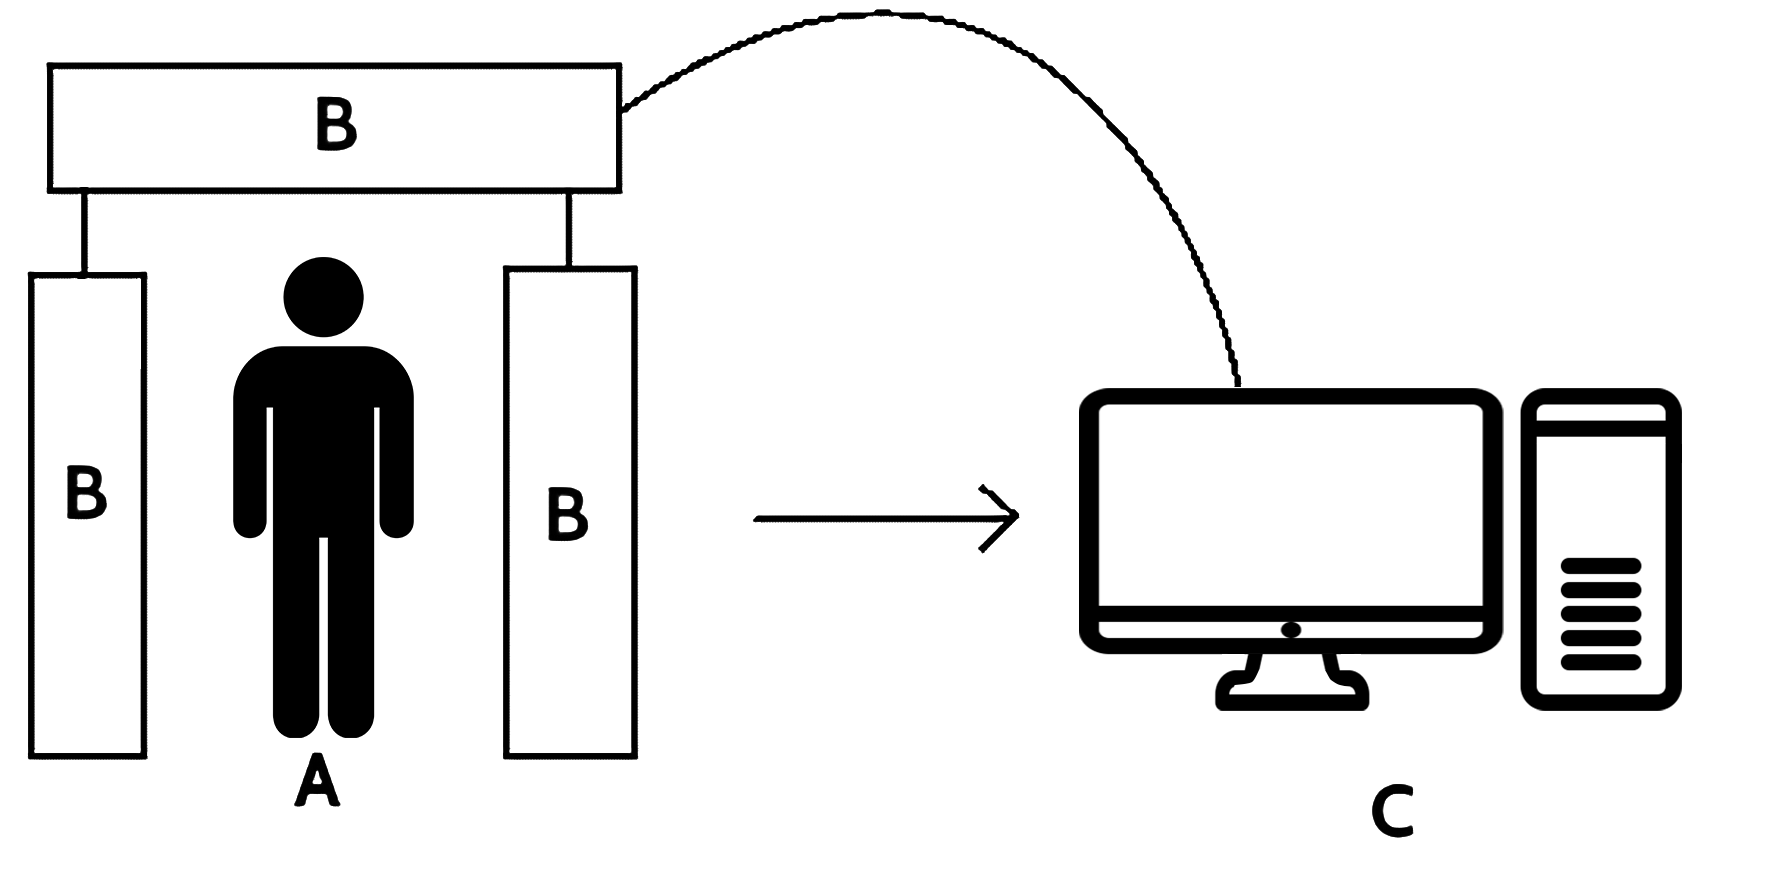
\includegraphics[width=0.8\textwidth]{kycia/BrainTransfer2.png}
 \caption{$A$---a human whose neural network is mapped by a device $B$. Using this mapping the model of the brain is constructed in $C$.}
 \label{Fig.BrainTransfer}
\end{figure}
%%%%
Assuming that the mapping by the machine $B$ can be undertaken accurately, the outcome $C$ is highly dependent on the nature of data $S$ stored in the brain of $A$. 

Three cases are as follows.


\textbf{Case 1---Brain data are stored in a classical physics structure.} In this case, a perfect copy of the data part of the brain can be made. The model of the brain---the copy--- can be made and no disruption to the original specimen $A$ (apart from the classical interaction of $A$ with measurement device $B$ which in principle can be done non-destructively) is made. As full information on the brain can be copied, the brain has no UA1 property. Besides, since in case of death or injury of the brain structures that store data disintegrate, therefore, no UA2 property is present. When the experiment of Fig. \ref{Fig.BrainTransfer} is performed, the two initially identical 'brains' (the specimen $A$ and the copied model $C$) will operate at the same time independently.


\textbf{Case 2---Brain data are stored in quantum physics structures.} No copy of the brain can be performed without altering it and therefore the brain cannot be copied. As a result, this brain has the UA1 property. Moreover, as quantum data are non-destructible, according to Theorem \ref{Th.NoDeleting} the brain also has the UA2 attribute. If this assumption is valid, then the experiment from Fig. \ref{Fig.BrainTransfer} will result in transferring data (as no copy is permitted) to the model $C$ and therefore transcendence. The original brain $A$ due to the destructive nature of measurement during the transfer will be altered and cannot be considered as the initial $A$. Only one fully functional brain equivalent to the initial $A$ brain will operate at a given moment. A question arises as to the extent to which the functionality of $A$ will be altered. Given that the quantum component is essential for consciousness, the `copy' operation changes the state $A$ and therefore potentially creates a `philosophical zombie'.


\textbf{Case 3---Brain data contains both classical and quantum information.} This case is a mixture of both the above cases. The classical part of the brain data can be copied and destroyed and therefore the brain cannot have UA1 and UA2 properties. However, the quantum part of the brain data possesses these two properties. The experiment of Fig. \ref{Fig.BrainTransfer} will transfer the quantum part to $C$ and alter it in $A$; moreover, it will copy the classical part of the brain to $C$. Thus, the specimen $A$ will not be the same as before the transfer due to altering the quantum part transferred to $C$. As a result, only one fully functional model of the brain equivalent to the initial state of $A$ will be present at a given time. The second brain (in $A$) will be altered due to the measurement of quantum data transferred to $C$. If the quantum component is essential for consciousness, then its alteration in $A$ during the copying process may lead to a `philosophical zombie'. However, if the quantum component is irrelevant for consciousness, then the copy can be sufficiently accurate to make it impossible to distinguish the copy $C$ and the original $A$.

%%%%
\begin{figure}
\centering
 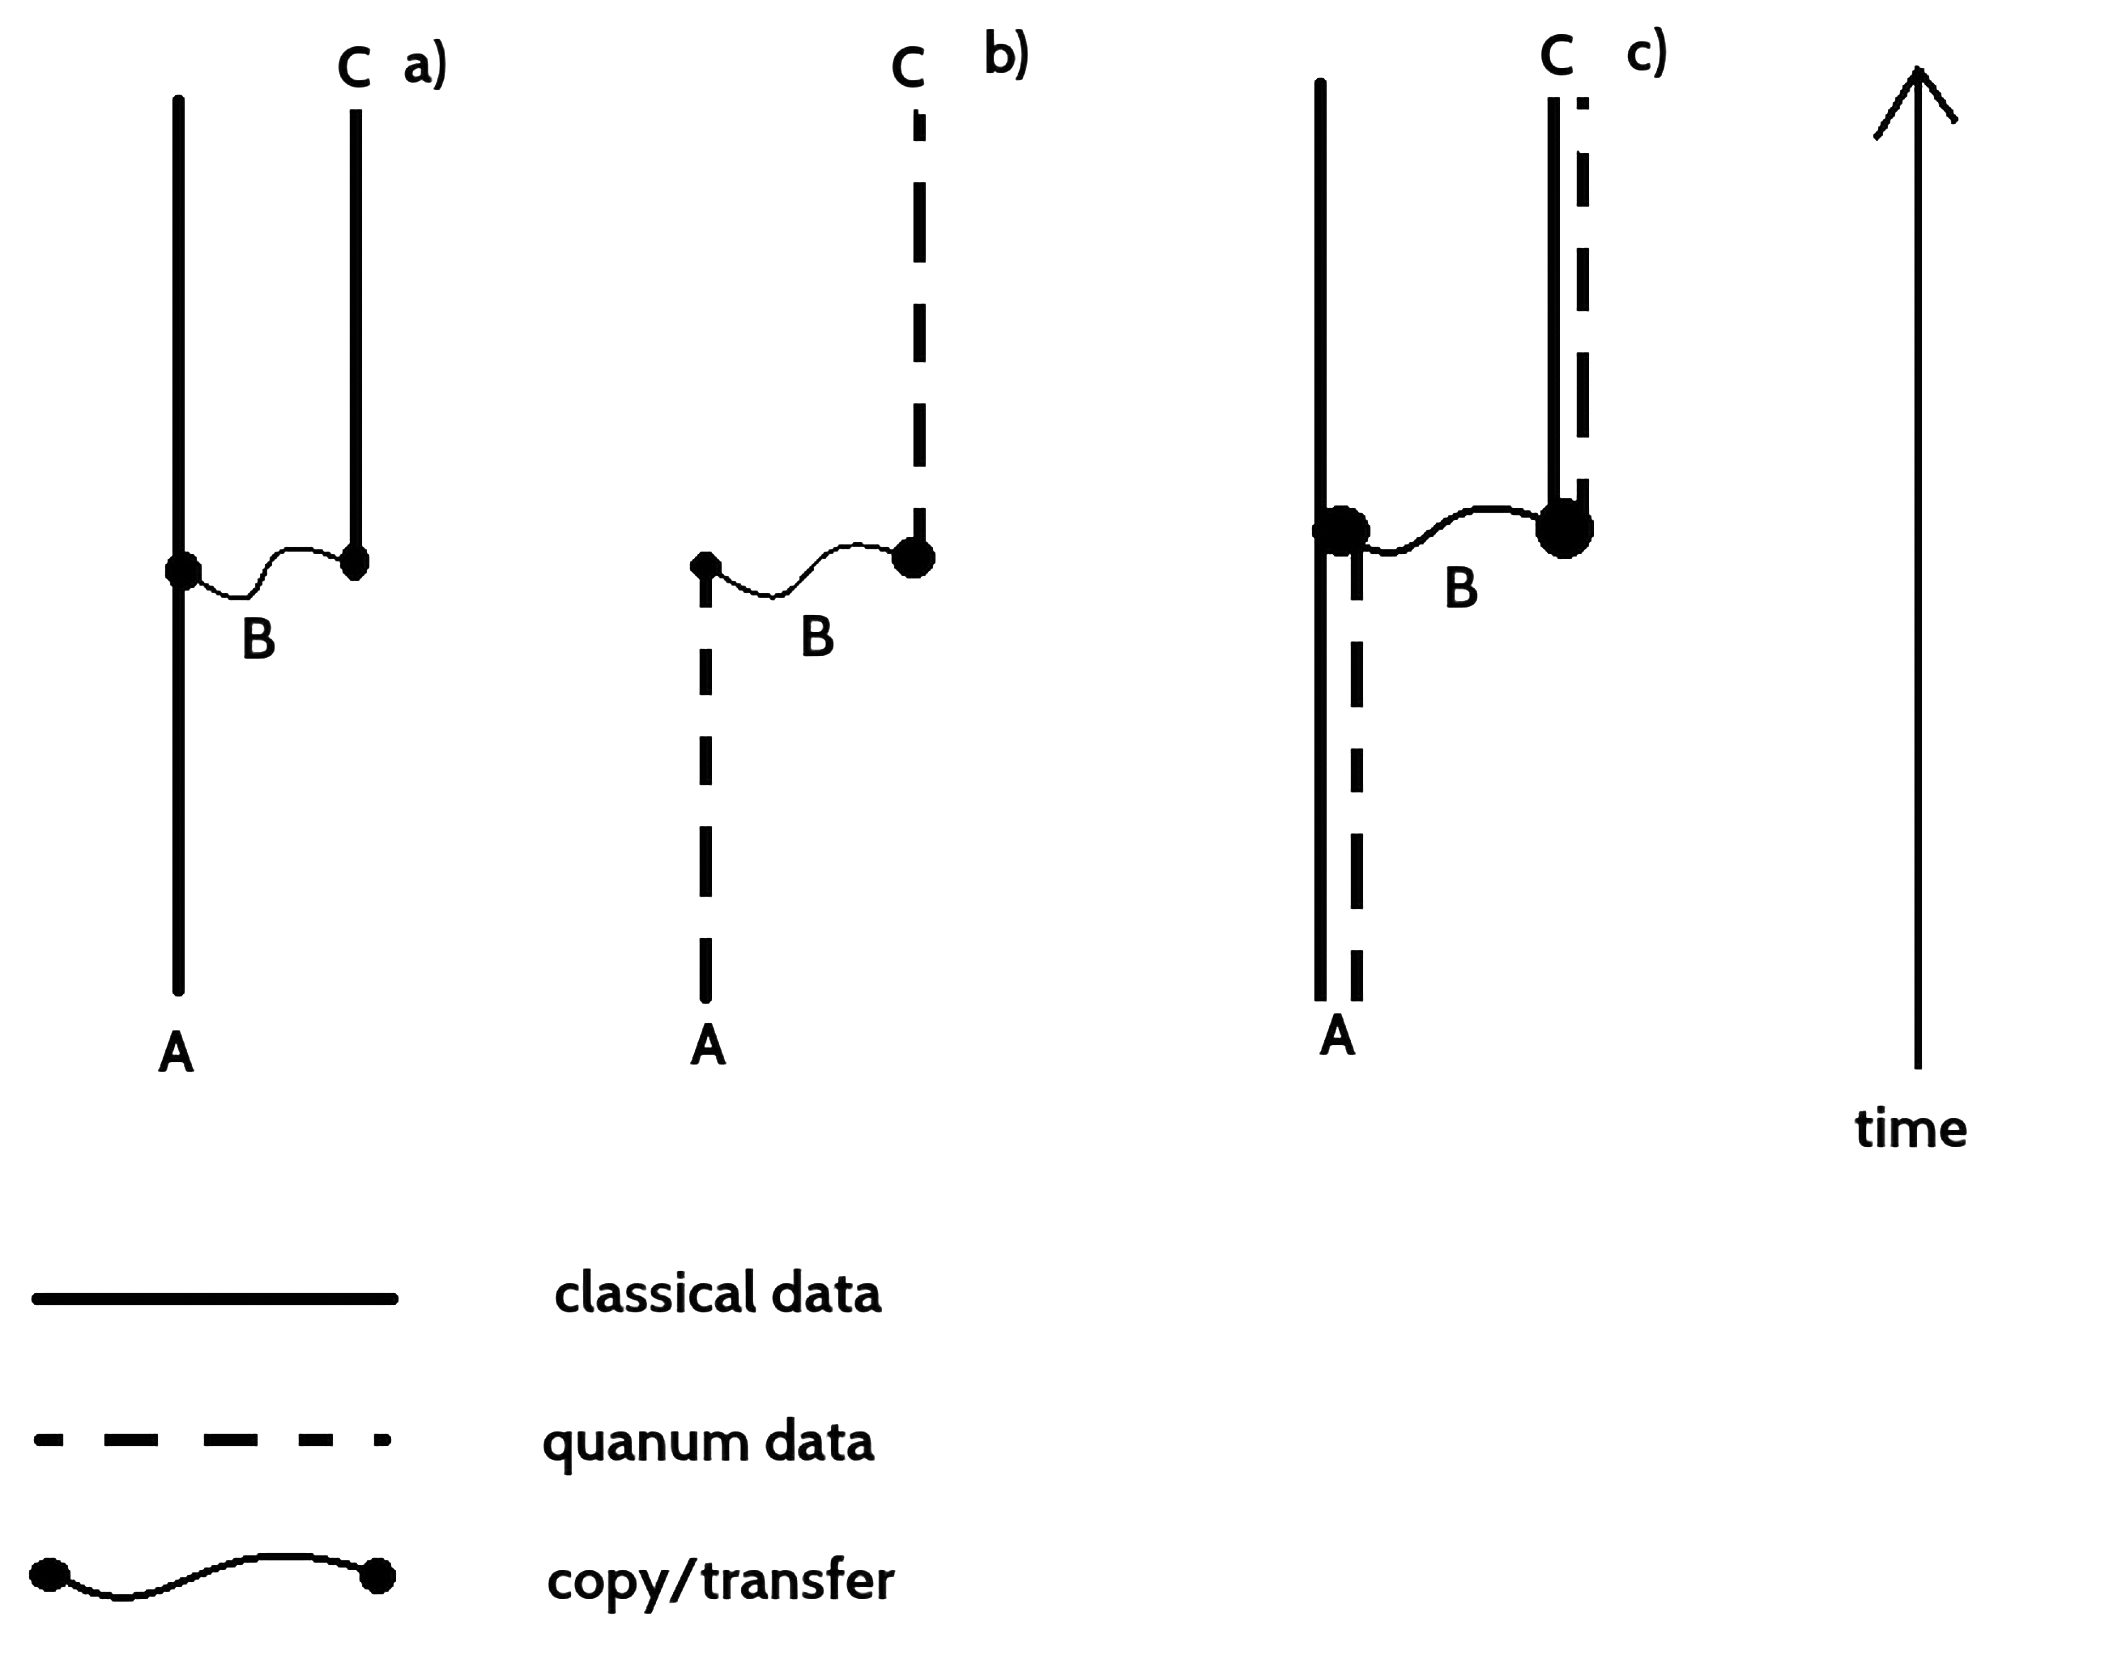
\includegraphics[width=0.7\textwidth]{kycia/TimeDiagram2.png}
 \caption{Case 1---a), Case 2---b) and Case 3---c) in time diagram. $A$- human, $B$- action of copy/transfer machine, $C$---simulator. One can observe that the quantum information is transfered and classical data copied. Quantum transfer alter original state.}
 \label{Fig.TimeDiagram}
\end{figure}
%%%%
These cases are presented in the time domain in Fig. \ref{Fig.TimeDiagram}.


For quantum data in the brain, one can perform copy with destruction, namely by measuring the quantum state of the brain (thereby altering this quantum state) and then creating a copy and restoring the brain's original state. In such a process, there is no continuity of existence of the original quantum state of the brain. However, there is a question as to whether it will be possible to set an altered brain quantum state $A$ to the original value before measurement. This depends on the complexity of the operation and the technology available. If the brain after quantum measurement can be set to the state before computation, then all quantum cases will have the same behaviour as in the classical case. 


As a conclusion from these cases, if the brain contains data that are quantum in nature, then it has properties UA1 and UA2.


The final subsection will present some remarks about the implications for metaphysical concepts.

%%%%%%%
\subsection{3.4. Metaphysical considerations}
%%%%%%%

The property UA1 (unable to be copied and therefore unique) does not imply indestructibility, defined by UA2. However, in the quantum case, both properties are present. Moreover, by UA2 property and by Theorem \ref{Th.NoDeleting}, the quantum state of the brain resides in the environment state after deletion and can be restored from it. If we assume that death is a quantum unitary deletion process, then the property UA2 describes some quantity that is preserved beyond the ceasing of the brain's computational functionality. We have attributed this to some part of the consciousness. However, the term 'soul' \parencite{Soul}, which has additional metaphysical connotations, is more accurate for this property. In this context, the environmental state is the storage for 'souls' attributed to the 'afterlife'.

In this presentation, we have used the terms 'soul' and 'afterlife' without any religious connotations: they are the brain's quantum and environmental states, respectively. However, there is some similarity with the concept of soul (the immortal part of a human) and the afterlife. 


If the brain operates solely on classical principles (or if the quantum component is irrelevant), then 'consciousness' is the proper term to use. In this case, the metaphysical part attributed to the 'soul' must be regarded as an additional property, if one exists. 





%%%%%%%%%%%%%%%%%%%%%%%%%%%%%%%%%%%%%%%%%%%%%%%%%%%%%%%%%%%%%%%%%%%%%%%%%%%%
\section{Conclusions}
%%%%%%%%%%%%%%%%%%%%%%%%%%%%%%%%%%%%%%%%%%%%%%%%%%%%%%%%%%%%%%%%%%%%%%%%%%%%
Under reasonable assumptions as to the computational brain model and by employing properties of classical and quantum information, the possibility of performing the brain copy has been investigated. Only quantum properties result in the existence of a part of the brain that cannot be copied (and is therefore unique) and that cannot be destroyed. In the process, this investigation has explained the possible outputs of hypothetical brain copy experiments.


%%%%%%%%%%%%%%%%%%%%%%%%%%%%%%%%%%%%%%%%%%%%%%%%%%%%%%%%%%%%%%%%%%%%%%%%%%%
%Acknowledgments
%%%%%%%%%%%%%%%%%%%%%%%%%%%%%%%%%%%%%%%%%%%%%%%%%%%%%%%%%%%%%%%%%%%%%%%%%%%
\paragraph{Acknowledgments}

The author would like to thanks Jacek Turnau for constructive feedback. The comments of Referees also made the paper clearer. 

The author was supported by the Ministry of Industry and Trade of the CR number CZ.01.1.02/0.0/0.0/19\_262/0019723, and the grant MUNI/A/0885/2019 of Masaryk University and would like to acknowledge COST CA18223 action for support. %broken phrase fixed - to consult with autor



\paragraph{Author's statement}
All speculations in the paper are only the author's statements and do not reflect the viewpoint of any institution and should not be associated with them. All presented statements are logical conclusions from the available scientific results and imposed assumptions. The paper is written in a good will and by preserving the highest scientific standards. This paper is not intended to offend anyone. It is written as an attempt to describe the still yet unformalized area of human activity.

\end{artengenv}
\label{kycia_ende}





\begin{artengenv}{Piotr Błaszczyk}
	{Galileo's Paradox and Numerosities}
	{Galileo's Paradox and Numerosities}
	{Galileo's Paradox and Numerosities}
	{Pedagogical University of Cracow, Institute of Mathematics}
	{Galileo's paradox of infinity involves comparing the set of natural numbers, $\N$, and the set of squares, $\{n^2:\, n\in\N\}$. Galileo \parencite*{ref_GG38},  by setting up a one-to-one correspondence, considers these sets  to have equal \textit{number} of elements. Then, he characterizes the set of squares as \textit{smaller} than the set of all numbers on the intuitive ground that ``there are many more numbers than squares.''  
	Finally, he concludes that infinities do not comply with the law of trichotomy when compared in terms of greater--lesser.
	
	Cantor's cardinal numbers provide a now-standard measure for sets. Cantor \parencites*{ref_C97}[Engl. transl.][]{ref_C15}  defines the relation greater--lesser and proves the law of trichotomy for these numbers. 
	When they apply to subsets of $\N$,   any set can be either finite or of the power $\aleph_0$. Although  $\N$  includes squares, these two sets are of the same cardinality.
	
	Cantor's ordinal numbers {measure}  well-ordered sets. Then, the same number $\omega$  identifies the order type of the sets  $\mathbb N$ and \mbox{$\{n^2:\, n\in\N\}$}.
	
	Benci and Di Nasso \parencite*{ref_BN19} introduce specific numbers called \textit{numerosities}  to  measure sets. In that theory,  the following claim is true: \textit{numerosity of A} $<$ \textit{numerosity of B}, whenever $A\subsetneq B$. Numerosities, like  ordinal numbers,  require some structure on measured sets called labels.
	
	In this paper, we present a simplified, self-contained version of the theory of \textit{numerosities} that applies to subsets of $\N$ with the \textit{natural} order and does not refer to labels. This theory complies with Galileo's presupposition that when $A\subsetneq B$, then
	the \textit{number} of  elements in $A$ is  smaller than the \textit{number}  of  elements in $B$. Specifically, we show that given the \textit{numerosity} of $\N$ is the specific hyperreal number $\alpha$, the \textit{numerosity} of the set of squares is the integer part of the number $\sqrt{\alpha}$, that is $\big\lfloor\sqrt{\alpha}\big\rfloor$, and  the inequality  $\big\lfloor\sqrt\alpha\big\rfloor<\alpha$ holds.
	
	In the second part, we discuss  Euclid's axiom \textit{The whole is greater than the part},  praised by founders of the numerosity theory,  and  Mancosu's \parencite*{ref_pm09},  the first study that introduced numerosities into a philosophical debate.  To this end, we embed number systems referred to in the paper---hyperreals, numerosities, Cantor ordinal numbers, and algebraic interpretation of Euclid's axiom---in the ordered field of Conway numbers.}
	{non-standard real numbers, numerosities, cardinal numbers, Galileo's paradox.}






%\newpage\tableofcontents
%\newpage
\section{Introduction}
\vspace*{-30pt}
\subsection{1.1. Galileo on infinities}
In  \textit{Discorsi e dimostrazioni matematiche: intorno à due nuoue scienze, attenenti alla mecanica \& i~movimenti locali\ldots{}} \parencite*{ref_GG38}, in a series of dialogues, Galileo Galilei discusses many topics in natural philosophy.  Whether a line consists of  points was then a routine question. 
Euclid's \textit{Elements} and Aristotles' \textit{Physics} set up that issue.  
Definition VII.2 of the \textit{Elements}, ``A number (is) a multitude 
(\foreignlanguage{polutonikogreek}{pl~hjos}) composed of units (\foreignlanguage{polutonikogreek}{mon'awn})'', ascertain numbers consist of units.  
The question was whether in geometry, the realm of continuity, points, defined by  I.1 ``A point is that of which there is no part'', could play a role analogous to units in arithmetic.
 Aristotles'  definition that  continuous objects are ``divisible into  infinitely (\foreignlanguage{polutonikogreek}{>ae'i}) divisible divisibles'' (\textit{Physics} VI.2) introduce infinity into the debate.


Galileo's position that magnitudes are composed of  \textit{non quanti} indivisibles drives him to the then-known paradox of infinity of parts of line segments. Yet, he
gives that discussion  a new push
by turning it into whether infinities, alike magnitudes, and numbers, are comparable in terms of greater-lesser.
His initial argument is simple:
Since one line can be greater than another, given each contains ``an infinite number of points'',  the infinity of points in the longer one is greater than the infinity of points in the shorter \parencite[see][30--33]{ref_GG56}. 

At this stage, greater-lesser does not mean set-subset relation. The idea of comparing line segments, rather than their lengths (measures), originates from the \textit{Elements}. It was self-evident in the 17\textsuperscript{th} century and prevailed until the 19\textsuperscript{th} century. The rise of the real number system enhanced the process of measuring 
magnitudes---lines by lengths, figures by areas, solids by volumes.  
Both in ancient Greek and 17\textsuperscript{th}-century mathematics, it was also evident,  that line segments were subject to the law of trichotomy (see section \S\,5.1 below). Thus, the point was whether infinities are subject to the same laws as then-common mathematical objects, such as line segments,  natural numbers, or ratios.

The idea that there is a variety of infinities,  one greater than another, puzzled the discussants.  Galileo  does not  reject the infinity, instead  he concludes that the law of  trichotomy does not apply in that domain:
``we cannot speak of infinite quantities as being the one greater or less than or equal to another'' \parencite[30]{ref_GG56}. 
To clarify this point, he involves natural numbers and states what later got the name Galileo's paradox of infinity.   
He sets up a one-to-one correspondence between the set of natural numbers, $\N$, and the set of squares, $\{n^2: n\in\N\}$; in this sense, respective infinities  are equal.
 He also observes that ``there are more numbers than squares''; in this sense, the former infinity is greater than the latter.  Here is the key part of this dialogue \parencite[33]{ref_GG56}:
 
\myquote{
If I should ask further how many squares there are one might reply truly that there are as many as the corresponding {number} of roots, since every square has its own root and every root its own square, while no square has more than one root and no root more than one square [...]. 
But if I inquire how many roots there are, it cannot be denied that there are as many as the numbers because every number is the root of some square. This being granted, we must say that there are as many squares as there are numbers because they are just as {numerous} as their roots, and all the numbers are roots
[...]  Yet at the outset we said that there are many more numbers than squares, since the larger portion of them are not squares. 
}

The conclusion is as follows: 
\myquote{
we can only infer that the totality of all numbers is infinite, that the number of squares is infinite, and that the number of their roots is infinite; neither is the number of squares less than the totality of all the numbers, nor the latter greater than the former; and finally the attributes \textit{equal}, \textit{greater}, and \textit{less}, are not applicable to infinite, but only to finite, quantities. When therefore Simplicio introduces several lines of different lengths and asks me how it is possible that the longer ones do not contain more points than the shorter, I answer him that one line does not contain more or less or just as many points as another, but that each line contains an infinite number \parencite[33]{ref_GG56}.
}


%Hence, on the one hand, the infinity of all numbers and  the infinity of all squares, are equal, in the sense one-to-one correspondence, on the other hand, the set of all numbers  is greater than the set of square, since it includes the later.  

In the dialogue that  follows, Galileo also argues that one can not compare finite and infinite in terms of 
greater--lesser, as that gives rise to new paradoxes; 
``And thus from your ingenious argument we are led to 
conclude that the attributes \textit{larger}, \textit{smaller}, and \textit{equal}
have no place either in comparing infinite quantities with each 
other or in comparing infinite with finite quantities'' \parencite[33]{ref_GG56}. 

\subsection{1.2. Cantor's  law of trichotomy for cardinal numbers}
Georg Cantor, in  philosophical 
digressions spread throughout his mathematical papers presents himself as the pioneer of a study of actual infinity. In his view,   only  Leibniz and Bolzano had approached the absolute infinity seriously before he did. His biographer, Joseph Dauben, in the very popular book \textit{Georg Cantor. His Mathematics and Philosophy of the Infinite} \parencite*{ref_jd}, upholds this legend. At present,  Cantor is generally considered the founding father of the mathematical study of infinity.  However,  there were pre-Cantorian theories of actual infinity developed within the tradition of geometrical optics, from Euclid, through Kepler to Descartes \parencite[see][]{ref_pb20}. And the real challenge for Cantor was  Euler's \textit{Introductio in Analysin Infnitorum} \parencite*{ref_LE48} which refers to the study of infinity in its very title and, obviously, the substance content. Since Euler's infinite numbers were inverses of infinitesimals, Cantor made endless attempts to dismiss these seemingly strange numbers \parencite[see][]{ref_bf}. Nevertheless, he neither mentioned Euler as the author of a competing theory of infinity, nor Galileo and his idea of equality of infinities based on one-to-one correspondence. 

Nowadays, Cantor's theory of cardinal numbers is a part of the common mathematical and philosophical education. Therefore, here, by referring to \parencite{ref_C97}, we note only the basic definitions related to Galileo's paradox.   Thus, the cardinal number of a set $M$, $\overline{{\overline M}}$, is equal to  the cardinal number of  a set $N$,
 $\overline{{\overline N}}$,  iff there is a one-to-one correspondence between these sets, $M\sim N$.   The relation greater--lesser does not reduce to the relationship of one set being a subset of another.  It is defined as follows:  $\overline{{\overline N}}< \overline{{\overline M}}$ iff there is $L\subset M$ such that $L\sim N$ and it is not the case that $N\sim M$.   Cantor managed to prove the law of trichotomy for cardinal numbers. Yet, it was far from trivial, as he observed:
\myquote{
We have seen that, of the three relations  $\textbf{a}=\textbf{b},\ \textbf{a}<\textbf{b},\ \textbf{a}>\textbf{b}$
each one excludes the two others. On the other 
hand, the theorem that, with any two cardinal 
numbers $\textbf{a}$ and $\textbf{b}$, one of those three relations must 
necessarily be realized, is by no means self-evident 
and can hardly be proved at this stage \parencites{ref_C97}[English translation after][90]{ref_C15}.\footnote{In the current set theory,  the law of trichotomy for cardinal numbers is equivalent to the Axiom of Choice. See \parencite[ch. 8, \S\,6.]{ref_km78}.}
}

At the turn of the 19\textsuperscript{th} and 20\textsuperscript{th} centuries, Cantor's theory of infinity reigned.  Although its definitions are not built on  theorems, as it sometimes happens in mathematics, people started to consider cardinal numbers as the indispensable measure of infinite sets.

Kurt G\"odel reinforced the belief that there is no alternative to Cantor's theory of infinite
numbers. 
In \parencite{ref_kg47}, he presents
cardinal numbers as extending the system of natural numbers $(\N,+, \cdot, 0, 1,<)$ and seeks
to show that ,,this extension can be effected in a uniquely determined manner.''

Nevertheless, there is still some  dissatisfaction: when we apply Cantor's theory to subsets of $\N$ there are only two possibilities there---a set can be either finite
or has the cardinality $\aleph_0$. 

Ordinal numbers provide another way of measuring infinite sets, yet they refer to well-ordered sets rather than bare sets. Cantor designed arithmetic for these numbers as well as the greater-lesser relation. In this case, the law of trichotomy does not relate to the Axiom of Choice  \parencite[see][ch. 7]{ref_km78}. Modern accounts of set theory introduce cardinal numbers as specific ordinal numbers \parencite[ch. 3]{ref_tj}.
Finite numbers, that is, elements of $\mathbb N$, are both cardinal and ordinal numbers, and in each case, they contribute the hierarchy greater-lesser.




\subsection{1.3. Numerosities}
In  the sections that follow, we present a theory that assigns  special numbers, called \textit{numerosities}, to subsets of $\N$ in  such a way that \textit{numerosity of A}$<$\textit{numerosity of B}, whenever $A\subsetneq B$. In this sense, \textit{numerosities} meet Gelileo's intuition that the relation greater--lesser between infinities agrees with the subset relation. 

The general theory of \textit{numerosities} is developed in \parencite{ref_BN19} as well as a variety of papers also authored by Vieri Benci and his collaborators. Below, we present its simplified version that applies only to subsets of $\N$. We define \textit{numerosities} as nonstandard natural numbers introduced through an ultrapower construction, where the \textit{numerosity} of $\N$ is a number $\alpha$ represented by the equivalence class $[(1,2,3,...)]$. 
Still, we need a bigger structure  to define numbers such as $\sqrt \alpha$ or $\alpha/2$. To this end, we introduce a field of nonstandard real numbers.

  To make this presentation self-contained, we start with the basics of the theory of ordered fields. Then, we proceed to the extension of the field of real numbers to the field of nonstandard reals. With these foundations, we can easily introduce \textit{numerosities} and demonstrate  theorems. 




\section{The basics of ordered fields theory}


A commutative field $(\F,+,\cdot,0,1)$ together with a total order $<$ is an ordered field when the sums and products are compatible with the order, that is
%\begin{eqnarray*}
%x<y &\Rightarrow& x+z<y+z,\\
%x<y,\, 0<z&\Rightarrow& xz<yz.
%\end{eqnarray*}
\[x<y \Rightarrow x+z<y+z,\ \ \ x<y,\, 0<z\Rightarrow x\cdot z<y\cdot z.\]

In any ordered field, we  define in a usual way an absolute value, $|x|$,  and a limit of  sequence,  
\[\lim\limits_{n\rightarrow\infty}a_n=g  \Leftrightarrow (\forall \varepsilon >0)(\exists k\in\N)(\forall n\in\N)(n>k \Rightarrow |a_n-g|<\varepsilon).\]


Note, however,  that while in real analysis the formula $\forall \varepsilon>0$
stands for $\forall \varepsilon\in\R_+$, in an ordered field,  it means
$\forall \varepsilon\in\F_+$. Moreover, in any field, whether Archimedean or non-Archimedean, indexes $k, n$ range over standard natural numbers $\N$. 

 The term $n$ is defined by
\[n=_{df}\underbrace{1 +1 + ... + 1}_{n - times},\]
while $\frac nm=_{df} n\cdot m^{-1}$. On this, basis we assume that any ordered field includes natural numbers, $\N$, and rational numbers, $\Q$. In fact, the field of fractions $(\Q,+,\cdot,0,1,<)$ is the \textit{smallest} ordered field.

In every ordered field, we can define the following subsets of $\F$:
\begin{eqnarray*}
 \mathbb L &= & \{x\in \F: (\exists n\in \N)(|x|<n)\},\\
 \mathbb A &=&   \{x\in \F: (\exists n\in \N)(\tfrac 1 n<|x|<n)\},\\
 \Psi             &=& \{x\in \F: (\forall n\in \N)(|x|>n)\},\\
 \Omega      &=& \{x\in \F: (\forall n\in \N)(|x|<\tfrac 1n)\}.
 \end{eqnarray*}

 The elements of these sets are called  limited, assignable,   infinite, and infinitely small numbers respectively.
Here are some obvious relationships between these kinds  of elements, we will call them $\Omega\Psi$ rules,
%In what follows we show some relations and dependencies we will refere to when interpreting Euler's writings.
%We can easily show  infinite numbers can be equally definied via  natural numbers, finite numbers, as well as assignable numbers
%It can be easily shown that the following relations hold (in short, $\Omega\Psi$ rules):
\begin{enumerate}\itemsep 0mm
\item[] $(\forall x, y\in\Omega)( x+y\in\Omega, x\cdot y\in\Omega)$,
\item[]  $(\forall x\in\Omega)( \forall y\in\mathbb L)( x\cdot y\in\Omega)$,
\item[] $(\forall x)(x\in \mathbb A\Rightarrow  x^{-1}\in\mathbb A)$,
\item[] $(\forall x\neq 0)(x\in\Omega  \Leftrightarrow \ x^{-1}\in\Psi)$.
\end{enumerate}


%\begin{equation} \Psi= \{x: (\forall a\in\A)(|x|>|a|)\}. \end{equation}
%\begin{equation} \Omega=\{x: (\forall a\in\A)(|x|<|a|)\}. \end{equation}
%\begin{equation}(\forall x, y\in\Omega)( x+y\in\Omega, xy\in\Omega) \end{equation}
%\begin{equation}(\forall x\in\Omega)( \forall y\in\mathbb A)( xy\in\Omega)\end{equation}
%\begin{equation}(\forall x)(x\in \mathbb A\Rightarrow  x^{-1}\in\mathbb A)\end{equation}
%\begin{equation}(\forall x\neq 0)(x\in\Omega  \Leftrightarrow \ x^{-1}\in\Psi),\end{equation}
%\begin{eqnarray*}(\forall x, y\in\Omega)&& x+y, xy\in\Omega,\\
%(\forall x\in\Omega)( \forall y\in\mathbb L)&&  xy\in\Omega,\\
%(\forall x\in \Omega)(\exists y\in\Psi)&& xy\in \mathbb L,\\
%(\forall x\neq 0) && x\in\Omega  \Leftrightarrow \ x^{-1}\in\Psi,\\
%(\forall x\in \mathbb A) &&  x^{-1}\in\mathbb A.
%\Omega=\{x: (\forall a\in \mathbb A)(|x|<|a|)\}
%\end{eqnarray*}

%Referring to the set $\Omega$, an equivalence relation is defined by
%\[x\approx y \Leftrightarrow x-y \in\Omega.\]
%We say that $x$ \emph{is infinitely close to} $y$, when the relation $x\approx y$ holds.


%Although we present the above relations within the modern framework, all of them were explicitly discussed in \parencite{Euler:55}, ch. 3.
%Next to $\Omega\Psi$ rules, it can also  be shown that $\Omega$ is the maximal ideal in the ring $(\mathbb L,+,\cdot,0,1)$ and the quotient ring $\mathbb L/{\Omega}$ is a field.  We do emphasize   $\Omega\Psi$  rules only because they are explicitly discussed in (Euler 1755);  see  \S \ below.


\subsection{2.1. Archimedean axiom}
When to the axioms of an ordered field we add the so-called Archimedean axiom, we obtain the class of
Archimedean fields.
Here are some equivalent forms of the Archimedean axiom:
\begin{enumerate}\itemsep 0mm
  \item [(A1)] $(\forall x,y\in \F)(\exists n\in\N)(0<x<y\Rightarrow n\cdot x>y)$,
  \item [(A2)] $(\forall x\in\mathbb F)(\exists n\in\N)(n>x) $,
  \item [(A3)] $\lim\limits_{n\to \infty} \frac 1n=0$,
  \item [(A4)] $(\forall x,y\in\mathbb F)(\exists q\in\mathbb Q)( x<y\Rightarrow x<q<y),$
\item [(A5)] For any Dedekind cut  $(A,B)$ of $(\F,<)$ obtains\footnote{For the remainder, a pair $(A,B)$
 of non-empty sets is a Dedekind cut of a totally ordered set $(X,<)$ iff: (1) $A\cup B=X$, %(2) $A\neq \emptyset, B\neq\emptyset$, (3)
 (2) $(\forall x\in A)(\forall y\in B)(x<y)$.}
$$(\forall n\in\mathbb{N})(\exists a\in A)(\exists b\in B)(b-a<\tfrac 1n),$$
\item[(A6)] $\Omega=\{0\}$.
\end{enumerate}



Versions A1 and A2 are well-known,  both in the mathematical as well as the historical context. A1 in the following form $(\forall x,y\in \F)(\exists n\in\N)(nx>y)$ originates from Euclid's \textit{Elements}, Book V, definition 4. It characterized the ancient Greek structure of magnitudes, specifically, line segments. In modern times, it is an axiom of Euclidean geometry.  Calculus courses usually present A3 as a theorem. However, it  follows from some versions of the continuity of real numbers, for example, C1 or C2 as presented below, 
or is explicitly included in other versions.
  A6 reveals that in a non-Archimedean field, the set of infinitesimals contains at least one positive element, say $\varepsilon$.
     Then, by $\Omega\Psi$ rules, $\tfrac \varepsilon n$, as well as, $n\cdot\varepsilon$   are also infinitesimals.

A3 provides a neat characterization of the non-Archimedean field: $(\frac 1n)$ is not a null-sequence.
In the field of formal power series (Laurent series), given $0<x<1$, $(x^n)$ is a null-sequence, that is $\lim\limits_{n\to \infty}x^n=0$. Moreover, it is a non-Archimedean and Cauchy-complete field \parencites[see][70]{ref_ce}[or][269--272]{ref_pb07}. The field of hyperreals, as defined in the next section, is also non-Archimedean and Cauchy-complete. Yet, due to the so-called saturation principle, there are no null sequences, except constant ones (or constant but a finite set).  

 
     
     
      %In addition,    inverses of these elements, i.e.  $\tfrac n \varepsilon$, $\tfrac 1 {n\varepsilon}$, also belong to that field and according to $\Omega\Psi$ rules, these are  infinitely large numbers. Let $\Omega_0$ stand for the set of non-zero infinitesimals, i.e.   $\Omega_0=\Omega\setminus\{0\}$.

%The  versions A1 to A6 above are equivalent within the framework of an ordered field while  some of them, for instance A1, apply to an ordered group
%$(\mathbb G, +,<)$. Then, the term $nx$ is defined by
%\[nx=_{df}\underbrace{x +x + ... + x}_{n - times}.\]
%
% We can also apply versions A4 and A5, provided the concept of fraction is interpretable in a group. Versions A3 and A6 involve the concept of an absolute value. While the very definition makes sense in any ordered group, some properties of the absolute value, such as
%$|x\cdot y|=|x|\cdot|y|$,
% require the order to be compatible both with sums and products. Hence, these versions need to be applied carefully.
%
% At the end of the 19\textsuperscript{th} century, a few non-Archimedean structures were introduced, however they contained rather exotic mathematical entities that provoked distrust.\footnote{\parencite{Ehrlich:06} provides a thorough overview of these structures.}
%We present a non-Archimedean group  made up  of then well-known objects, namely complex numbers; the simplicity of the model makes us wonder why it was not involved in the dispute concerning infinitesimals.
%
%Let $(\mathbb C,+,0,\prec)$ be the additive group of complex numbers with the lexicographical order, i.e.,
%\[a+bi\prec  c+di \Leftrightarrow a<c \vee  (a=c,\,b<d).\]
%
% The order is compatible with sums,  although  not  with products. One can easily show that
% $0\prec i\prec 1$,
%  moreover,   for every natural number $n$ the inequality $ni\prec 1$ holds. The set $\{ri:r\in \R\}$ includes  infinitesimals of the group $(\mathbb C,+,0,\prec)$.\footnote{\parencite{Blaszczyk:13b} provides historical account of the Archimedean axiom, from Euclid and Archimedes, through Heiberg's edition of Greek text, to the 19\textsuperscript{th} century theories of magnitudes developed by Stolz, Weber, H\"older and others. }
%\end{document}

\subsection{2.2. Real numbers}

 The field of real numbers   is  defined as a commutative ordered field $(\mathbb F,+,\cdotp,0,1,<)$ in which
 every Dedekind cut $(L,U)$ of $(\F,<)$ satisfies the following condition:
\begin{equation}\tag{C1}(\exists x\in\F)(\forall y\in L)(\forall z\in U)(y\leq x\leq z).
\end{equation}


Here are some  equivalent forms of C1:

\begin{enumerate}\itemsep 0mm
\item [(C2)] If $A \subset \F$ is a nonempty set which is bounded above, then there exists $a \in \F$ such  that  $a = \sup A$.
\item [(C3)] The field  is Archimedean and every Cauchy (fundamental) sequence $(a_n)\subset \F$  has a limit in $\F$.
\item[(C4)] The field  is Archimedean  and
 if $\big\{A_{n}|\ n\in\mathbb{N}\ \!\big\}\subset \F$ is a family of descending, closed line segments, then $\bigcap\limits_{n\in\mathbb{N}} A_{n}\not=\emptyset.$
\end{enumerate}


%Any equivalent form of C1  usually gets the name of {continuity} or {completeness},  and then the real numbers system is called the {continuous ordered field} or the {complete ordered field}. The version C2 is also known as {Dedekind completeness} or the {least upper bound} (LUB) principle, whereas   the second part of C3 is called  Cauchy completeness.  Since Dedekind and Cauchy completeness are not equivalent,  we prefer to use more specific names like Dedekind cut  or LUB principle.

The above definition applies the theorem that every two ordered fields satisfying C1 are isomorphic. In this sense, the field of real numbers is the unique, complete ordered field. Moreover, any Archimedean field is isomorphic to a subfield of real numbers.  As a result, any field extension of real numbers is non-Archimedean and includes infinitely small and infinite numbers.  
\section{The field of hyperreals}

In this section, we provide a specific field-extension of real numbers, namely a field of hyperreals (non-standard real numbers). Since \parencite{ref_RA}, many different approaches to non-standard reals have been developed. The one presented below is based on the so-called ultrapower construction.  The set of hyperreals  $\R^*$  is defined as the quotient class of the set of sequences of real numbers, $\R^{\N}$, with  respect to a specific relation defined on the set of indexes $\N$. We begin with this relation.


\subsection{3.1. Ultrafilter on the set $\N$}

 We start with
 the definition of an ultrafilter  on  $\N$ and present some basic results concerning ultrafilters.

  \textbf{Definition 1} A family of sets $\mathcal U\subset \mathcal P (\N)$ is an
  ultrafilter on $\N$ if (1) $\emptyset \notin \mathcal U$, (2) if $A,B\in\mathcal U$,
   then $A\cap B\in\mathcal U$, (3) if $A\in\mathcal U$ and $A\subset B$,
   then $B\in\mathcal U$, (4) for each  $A\subset \N$, either $A$ or its
   complement $\N\setminus A$ belongs to $\mathcal U$.

%It follows from this definition that either the set of odd numbers or the set of even numbers belongs to an ultrafilter.

   Take the family of  sets with  finite complements,
   \[\{A\subset\N:  \N\setminus A\ \ \mbox{is\ finite}\}.\]

It  is usually called the Fr\'{e}chet  filter on $\N$. Indeed, it obviously  satisfies conditions (1)--(3) listed in  Definition 1. Note, however, that neither the set of odd numbers nor the set of even numbers has a finite complement, hence, the Fr\'{e}chet  filter is not an ultrafilter.
   Still, by  applying the Axiom of Choice it can be  extended to an
ultrafilter. In what follows, let $\mathcal U$ be a fix ultrafilter on $\N$ which extends the
 Fr\'{e}chet  filter.\footnote{Since we apply the fixed ultrafilter, we can refer to the field, rather than a field of hyperreals.    Assuming the continuum hypotheses, $\R^*$  is unique up to isomorphism, that is,  it does not depend on a choice of an ultrafilter extending the Frechet filter.}


 Thus, we know that for every $k\in\N$, the family $\mathcal U$ includes the set
\[\N\setminus \{0,1,2,...,k\},\]
since  sets of this kind belong to the Fr\'{e}chet  filter.  Moreover, the set $\N$ also belongs to $\mathcal U$, since it belongs to the  Fr\'{e}chet  filter.
Next,  due to the condition (4) of Definition 1, for any subset $A$ of $\N$, either $A$, or $\N\setminus A$
belongs $ \mathcal U$. We apply this fact to prove, e.g. an equivalence  (1), as explained below.
Finally, it can be shown that the following proposition holds.

\textbf{Theorem 1} For any subsets $A_1,...,A_n$ of $\N$ such that $A_i\cap A_j=\emptyset$, $i\neq j$. If
$\bigcup_{i=1}^{n} A_i\in\mathcal U$, then  $A_i\in \mathcal U$ for exactly one $i$ such that $1\leq i\leq n$.

By applying this proposition, one can show that relations $<^*$ defined on the set $\R^*$ and $\N^*$ are actually total orders.

\subsection{3.2. Extending the field of real numbers}

In this section, we sketch  how to extend the field of real numbers
$(\R,+,\cdot,0,1,<)$  to a non-Archimedean field of
the hyperreals.\footnote{For details, consult \parencites{ref_BM}{ref_pb16}.} The set $\R^*$  is defined as the quotient class of $\R^{\N}$ with
 respect to the following relation
\[(r_n)\mathcal \equiv (s_n) \Leftrightarrow \{n\in\N: r_n=s_n\}\in \mathcal U.\]

Thus, $\R^*=\R^{\N}/_{\mathcal U}$. Clearly, the equality of hyperreals is defined by
\begin{equation}[(r_n)]= [(s_n)] \Leftrightarrow \{n\in\N: r_n=s_n\}\in \mathcal U. \end{equation}

It means that when sequences  $(r_n), (s_n)$ agree on a set of indexes that belongs to $\mathcal U$, 
they determine the same hyperreal number.  For example, suppose that the set of even numbers belongs to the ultrafilter, 
$\{2n: n\in \N\}\in\mathcal U$. If $r_{2n}=s_{2n}$, for every $n$, then $[(r_n)]=[(s_n])$. Therefore, specifically, the following equality holds
\[[(r_n)]=[(0,2,0,4,0,6,...)]=[(1,2,3,4,5,6,...)]=[(s_n)],\]
where the sequence $(s_n)$ is defined by $s_n=n$, and the sequence $r_n$ is defined by $r_n=n$, for even $n$, and
$r_n=0$, for odd $n$.


New sums and products are defined pointwise, that is
\[[(r_n)]+^*[(s_n)]=[(r_n+s_n)],\ \    [(r_n)]\cdot^*[(s_n)]=[(r_n\cdot s_n)].\]

New total order is defined by
\[[(r_n)]<^*[(s_n)]\Leftrightarrow \{n\in\N: r_n<s_n\}\in\mathcal U.\]

Hence, the product and sum of hyperreals $[(r_1,r_2,...)]$ and $[(s_1,s_2,...)]$ gives
$[(r_1\cdot s_1,r_2\cdot s_2,...)]$, and  $[(r_1+ s_1,r_2+ s_2,...)]$ respectively.
The relation
$[(r_1,r_2,...)]<^*[(s_1,s_2,...)]$ holds when, for example, the set $\{n\in\N: r_n<s_n\}$ equals $\N$ minus some finite set (though the definition of order $<^*$  includes also  other cases).


Standard real number, $r\in\R$, is represented by the class $[(r,r,r,...)]$, i.e., the class of a constant sequence $(r,r,r,...)$. Note that the sequence representing standard real number, e.g. 1, can take the same value from some index on, for example
\[1=[(1,1,1,1...)]=[(0,0,1,1,...)].\]

Owing to the above definitions,  we employ the same symbols for real numbers in the standard and non-standard context; we will also employ the same symbols for sums, products and order relation in the standard and non-standard context.

It follows from the notion of ultrafilter that the following relation holds
\begin{equation}[(r_n)]\neq [(s_n)]\Leftrightarrow \{n\in \N:\ r_n\neq s_n\}\in\mathcal U.\end{equation}

Due to this fact, we can control, e.g. an inequality such as this one $[(r_n)]\neq 0$. This fact, in turn, enables to show that the quotient structure is really an ordered field.



In the next section, we  consider hyperreal numbers represented by sequences of natural numbers, that is $[(n_j)]$, where $(n_j)\subset \N$, for instance
\begin{equation}\alpha=[(1,2,3,...)]=[(n)].\end{equation}

According to the definition of product, we have
\[\alpha^2=[(1,2,3,...)]\cdot[(1,2,3,...)]= [(1^2,2^2,3^2,...)]=[(n^2)].\]

Then, the hyperreal number $\frac \alpha 2$ is determined by the following equalities
\[\frac \alpha 2=[(1,2,3,...)]\cdot [(\tfrac 12,\tfrac 12,\tfrac 12,...)] =\big[\big(\tfrac 12,\tfrac 22,\tfrac 32,...\big)\big]=\big[\big(\tfrac n2\big)\big].\]

Similarly, that  is point-wise,  we define the hyperreal number $\sqrt{\alpha}$, namely
\[\sqrt\alpha =\big[\big(\sqrt 1,\sqrt 2,\sqrt 3,...\big)\big]=\big[\big(\sqrt n\big)\big].\]

In a similar way, the floor function  is defined, namely
\[\big\lfloor [(r_j)]  \big\rfloor=[(\lfloor r_j  \rfloor)].\]

Hence, hyperreal numbers  such as
\[\Big\lfloor \frac\alpha 2 \Big\rfloor\ \ \mbox{and}\ \ \big\lfloor \sqrt\alpha\big\rfloor,\]

are represented by sequences of natural numbers, namely
\[\Big\lfloor \frac\alpha 2 \Big\rfloor= \big[\big(\big\lfloor \tfrac n2\big\rfloor\big)\big],\ \ \ \big\lfloor \sqrt\alpha\big\rfloor=  \big[\big(\big\lfloor\sqrt n\big\rfloor\big)\big].   \]

More specifically,
  \[\Big\lfloor \frac\alpha 2 \Big\rfloor= \Big\lfloor\big[\big(\tfrac 12,\tfrac 22,\tfrac 32,...\big)\big]\Big\rfloor= \big[\big(\big\lfloor \tfrac n2\big\rfloor\big)\big]     =[(0,1,1,2,2,3,3,...)],        \]
\[  \big\lfloor \sqrt\alpha\big\rfloor=  \big[\big(\big\lfloor\sqrt n\big\rfloor\big)\big]=
[(\sqrt 1,1,1,\sqrt 4,2,..., 2,\sqrt 9,3,...,3,\sqrt{16},4,...)].   \]

Note that with natural numbers, the following equalities obtain $\lfloor \frac n2 \rfloor + \lfloor \frac n2 \rfloor=n$ or
$\lfloor \frac n2 \rfloor + \lfloor \frac n2 \rfloor +1=n$,
 depending on whether $n$ is even or odd. Similarly, $\Big\lfloor \frac\alpha 2 \Big\rfloor +\Big\lfloor \frac\alpha 2 \Big\rfloor=\alpha$ or $\Big\lfloor \frac\alpha 2 \Big\rfloor +\Big\lfloor \frac\alpha 2 \Big\rfloor+1=\alpha$, depending on whether the set of even numbers belongs or not  to the ultrafilter $\mathcal U$. More specifically,
suppose the set of even numbers belongs to $\mathcal U$. It means that for any sequence $(r_n)$, only elements with 
even indexes, $r_{2k}$, determine the number $[(r_n)]$, as explained above. Now,
 
 \[\Big\lfloor \frac\alpha 2 \Big\rfloor +\Big\lfloor \frac\alpha 2 \Big\rfloor=[(0,\textbf{2},2,\textbf{4},4,\textbf{6},6,... )]=[(1,\textbf{2},3,\textbf{4},5,\textbf{6},...)]=\alpha.\]
 
  
% The final equality obtains because sequences $(0,2,2,4,4,...)$ and $(1,2,3,4,...)$ agree on the set of indexes
% $\{2n:\ n\in\N\}$.
 
% Yet,  we skip
% a  discussion  needed to justify this claim.

For the sake of completeness, suppose the set of odd numbers belongs to $\mathcal U$. Given this, elements with odd indexes, $r_1, r_3, r_5,...$ determine the number $[(r_n)]$. In this case,
 \[\Big\lfloor \frac\alpha 2 \Big\rfloor +\Big\lfloor \frac\alpha 2 \Big\rfloor+[(1,1,1,...)]=
 [(\textbf{1},3,\textbf{3},5,\textbf{5},...)]=[(\textbf{1},2,\textbf{3},4,\textbf{5},...)]=\alpha.  \]
 
 We will refer to these results in section \S\,4.1(3), discussing the numerosity of the set of even numbers.

\subsection{3.3. Extending natural numbers}
In this subsection, we apply the ultrapower construction, as explained above, to natural numbers $(\N,+,\cdot,0,1,<)$. As a result, we obtain the nonstandard (and uncountable) model of Peano arithmetic $(\N^*,+,\cdot,0,1,<)$. Thus, the set $\N^*$  is  the quotient class of $\N^{\N}$ with
 respect to the  following relation
\[(n_j)\mathcal \equiv (m_j) \Leftrightarrow \{j\in\N: n_j=m_j\}\in \mathcal U.\]

New sums and products are defined pointwise,
 new total order is defined by
\[[(n_j)]<^*[(m_j)]\Leftrightarrow \{j\in\N: n_j<m_j\}\in\mathcal U.\]

A standard natural number, $n\in\N$, is represented by the class $[(n,n,n,...)]$.
 Like in the case of hyperreals, we employ the same symbols for natural numbers, as well as for their sums, products and order, in the standard and non-standard context.


Again, from the fact that the Fr\'{e}chet filter is the subset of $\mathcal U$, it follows that both the constant sequence $(2,2,2,...)$, and a  sequence $(n_j)$  which on a finite set of indexes $A$ takes $0$, and for other indexes takes $2$,
i.e.,
\[n_j=
\left\{\begin{array}{cc}
0, & \mbox{for $j\in A$}, \\
2, & \mbox{\ \ \ \ \,for $j\in\N\setminus A$},
\end{array} \right.\]
represent number $2$,
\[[(2,2,2,...)]=2=[(n_j)].\]

For the rest of our presentation, we call nonstandard natural numbers numerosities,
 and  give a special role for  the number $\alpha$, as defined by formula (3): we will show that $\alpha$ is the numerosity of the set $\N$. 
 %In fact, not all  nonstandard natural numbers, but only those  smaller than $\alpha$will play the role of a measure of a subset of $\N$.

To unify developments of this and the previous sections, we can define nonstandard natural numbers as a subset of the set of hyperreals as follows
\[\N^*=\{[(n_j)]\in\R^*\,|\, \{j\in\N\,|\,n_j\in\N\}\in\mathcal U\}.\]

It is up to the reader to decide which option he/she finds easier to follow.\footnote{When $A\subset \R$, then $A^*$
is defined by  $A^*=\{[(r_j)]\in\R^*\,|\, \{j\in\N\,|\,r_j\in A\}\in\mathcal U$\}. }

 




\section{Numerosities}
In this section, we present a simplified version of the theory of numerosities, as developed in \parencite{ref_BN19}. It considers subsets of $\N$ only.
Still, it exemplifies an alternative to  Cantor's theory of cardinal numbers. Within the Cantor system, every subset of $\N$ is either finite or has the cardinality $\aleph_0$, 
that is, for every $A\subset\N$, either $A\sim\N$ or $A\sim n$, for some $n$.
The theory developed by Vieri Benci and Mauro Di Nasso gives the same results regarding finite sets. Yet,  infinite subsets of $\N$  have smaller numerosity than $\N$.

We present numerosities as hyperreals ascribed to bare sets.  \parencite{ref_BN19} considers the so-called labeled sets.  \parencite{ref_BN14}, \parencite{ref_BN15} introduce numerosities in the context of  measure theory. Section 4.2 compares these attitudes.

\subsection{4.1. How to measure subsets of  $\N$ by numerosities}
 The key role in  Benci and Di Nasso's theory plays the way how numerosities are ascribed to subsets of $\N$.
 Here is this definition \parencite[279]{ref_BN19}).

Let $A$ be a subset of $\N$. We define a function
$\varphi_A:\N\mapsto\N_0$, by
\begin{equation}\varphi_A(n)=\overline{\overline{\{a\in A\ |\ a\leq n\}}}.\end{equation}

$\N_0$ means $\N\cup\{0\}$. When the set   $\{a\in A\ |\ a\leq n\}$ is empty, then $\varphi_A(n)=0$.

Usually, the symbol  $\overline{\overline{X}}$ stands for the cardinal number of the set $X$. Here it represents a   natural number, since for  every $n$, the set $\{a\in A\ |\ a\leq n\}$ is finite. Thus, we may interpret the symbol $\overline{\overline{\{a\in A\ |\ a\leq n\}}}$ as follows: \textit{how many elements of the sets $A$ are less or equal to $n$}.



\textbf{Definition 2} \parencite[280]{ref_BN19} The numerosity of the set $A$ is the nonstandard natural number $\nu_\alpha (A)$ represented by the sequence $(\varphi_A(n))$, that is
\begin{eqnarray*}\nu_\alpha (A) &=& [(\varphi_A(n))],\\
                                   &=& [(\varphi_A(1), \varphi_A(2), \varphi_A(3),...)].
                                                         \end{eqnarray*}

%$\nu_\alpha (A)=(\varphi_A(n))$ 
In this context, the index $\alpha$ has no mathematical meaning. By $\nu_\alpha (A)$ we refer to a notational convention applied by Benci and Di Nasso. 


Here are some examples. 1) Let us start  with  finite sets, e.g. a  two--elements set
 $A=\{k, l\}$, with $k<l$. We have,
\[\varphi_A(n)=
\left\{\begin{array}{ccc}
0, & \mbox{for $n<k$}, \\
1, & \ \ \ \ \ \mbox{for $k\leq n<l$},\\
2,  & \mbox{for $l\leq n$}.
\end{array} \right.\]



Since for all but finite number of $n$ we have $\varphi_A(n)=2$, the numerosity of $A$ equals 2, that is $\nu_\alpha (A)=2$.

In a similar way, we  obtain that numerosity of the set $A=\{a_1,...,a_k\}$ equals $k$.

2) Now, we  assign a numerosisty to the set of natural numbers $\N$. To this end, 
  observe that  $\varphi_{\N}(n)=n$, for every $n$. Hence, the sequence  $(\varphi_{\N} (n))$ is $(1,2,3,...)$, and
\[\nu_\alpha (\N)=[(1,2,3,...)]=\alpha.\]

This fact explains the role of the index $\alpha$: it is the numerosity of the set $\N$ and other numerosities rely on this basic fact.


3) Now, let us determine the numerosity of the set of even numbers $\mathbb E=\{2n:\ n\in\N\}$. One can easily  figure our the first terms of the sequence $(\varphi_{\mathbb E}(n))$. These are as follows
\[\varphi_{\mathbb E}(1)=0,\ \varphi_{\mathbb E}(2)=1,\ \varphi_{\mathbb E}(3)=1,\ \varphi_{\mathbb E}(4)=2,\ \varphi_{\mathbb E}(5)=2,...\]

Thus, $(\varphi_{\mathbb E}(n))=(0,1,1,2,2,3,...)$, and, finally
\[\nu_\alpha (\mathbb E)=[(0,1,1,2,2,3,...)]=  \Big\lfloor \frac\alpha 2 \Big\rfloor.   \]

The numerosity of the set of odd numbers, $\mathbb O=\{2n-1:\ n\in\N\}$, is as follows
\[\nu_{\alpha}(\mathbb O)=[(1,1,2,2,3,3,...)].\]

If the set of even numbers belongs to $\mathcal U$, then
\[\nu_{\alpha}(\mathbb O)=[(1,1,2,2,3,3,...)]=[(0,1,1,2,2,3...)]=\Big\lfloor \frac\alpha 2 \Big\rfloor.\]

If the set of odd numbers belongs to $\mathcal U$, then
\[\nu_{\alpha}(\mathbb O)=[(1,1,2,2,3,3,...)]=[(1,2,2,3,3,...)]=\Big\lfloor \frac\alpha 2 \Big\rfloor+1.\]

Regardless of whether the set of even or odd numbers belongs to $\mathcal U$, the equality holds
\[ \nu_\alpha (\mathbb E)+ \nu_{\alpha}(\mathbb O = [(0,1,1,2,2,3,...)]+ [(1,1,2,2,3,3,...)]=\alpha. \]

4) By induction, we can prove the general rule
\[A\subseteq B\Rightarrow \nu_\alpha (A)\leq\nu_\alpha (B).\]

Yet, below we demonstrate a more strict result, namely
\begin{equation}A\varsubsetneq B\Rightarrow \nu_\alpha (A)<\nu_\alpha (B).\end{equation}


Set $n_0=min(B\setminus A)$. Then $\varphi_B(n_0)=\varphi_A(n_0)+1$, and $\varphi_A(n)=\varphi_B(n)$, for every $n<n_0$. Moreover, $\varphi_B(n)-\varphi_A(n)\geq 1$, for every $n\geq n_0$. As a result
\[\{ n\in\N\mid\varphi_A(n)<\varphi_B(n)\}=\N\setminus\{ 1, 2, \ldots, n_0-1\}.\] 

Since $\N\setminus\{ 1, 2, ... ,n_0-1\}\in\mathcal U$, we get $\nu_{\alpha}(A)<\nu_{\alpha}(B)$. 

According to Benci and Di Nasso, formula (5) justifies the old law \textit{The whole is greater than the part}, even when applied to infinite sets. In our account, rule (5) applies to subsets of $\N$. 
%Still,  the domain of numerosities can be extended to the subsets of real numbers.



Let us  exemplify formula (5). Let $B=\N\setminus\{1,2,3\}$, that is $B=\{n\in\N: n\geq 4\}$. Then   $\nu_{\alpha}(B)=[(0,0,0,1,2,3,\ldots)]$. Clearly, 
$$\nu_{\alpha}(B)=[(0,0,0,1,2,3,\ldots)]<[(1,2,3,4,5,6,\ldots)]=\nu_{\alpha}(\N).$$ 

Moreover, 
\[[(0,0,0,1,2,3,\ldots)]+[(3,3,3,...)]=[(3,3,3,4,5,6,\ldots)]=\alpha.\]

It means, that
\[\nu_{\alpha}(B)=\alpha-3.\]

Generally, when an arithmetic formula defines the subset of $\N$,  we can determine its numerosity. 
Below, we exemplify this claim.


5) Let us calculate the numerosity of the set of squares $\{n^2:\ n\in\N\}$ that plays the key role in the Galileo's paradox. Now,
\[A=\{1,4,9, 16,..., n^2,...\}.\]
Here are first values of the function $\varphi_A$:
\begin{itemize}
\item []$\varphi_{A}(1)=\varphi_{A}(2)=\varphi_{A}(3)=1$,
\item []$\varphi_{A}(4)=...=\varphi_{A}(8)=2$,
\item []$\varphi_{A}(9)=...=\varphi_{A}(15)=3$,
\item []$\varphi_{A}(16)=...=\varphi_{A}(24)=4.$
\end{itemize}

We can easily check the that the sequence $(\varphi_{A}(n))$ represents the number 
\[  \big\lfloor \sqrt\alpha\big\rfloor=  \big[\big(\big\lfloor\sqrt n\big\rfloor\big)\big]=
[(1,1,1,\sqrt 4,2,2,2,2,\sqrt 9,3,...,3,\sqrt{16},4,4,...)].   \]

The number $\sqrt \alpha$ is hyperreal. Depending on whether the set of squares $\{n^2:n \geq 1\}$  belongs to the ultrafilter  $\mathcal U$,  it  is or is not a nonstandard natural number. Therefore, we define  the numerosity of $A$ as 
$\big\lfloor \sqrt\alpha\big\rfloor$ rather than simply $\sqrt \alpha$. Since $\alpha$, $\sqrt \alpha$, and $\big\lfloor \sqrt\alpha\big\rfloor$ are infinite elements of the field of hyperreals (specifically they are greater than $1$), the inequalities 
\[\big\lfloor \sqrt\alpha\big\rfloor \leq \sqrt \alpha<\alpha\]
 follow from the general laws of an ordered field. 
 
 6) Finally, let observe that the case of the numerosites of the set of even numbers and the set of squares represent more general rules, namely \parencite[286]{ref_BN19}
 
 when $A=\{nk:\ n\in\N\}$, then $\nu_\alpha(A)=\big\lfloor \frac \alpha k\big\rfloor$,
 
 when $A=\{n^k:\ n\in\N\}$, then $\nu_\alpha(A)=\big\lfloor \sqrt[k]{\alpha} \big\rfloor$.
 \hfill{$\Box$}


\subsection{4.2. Labels and non-Archimedean valued finitely additive measures}

In \parencite{ref_BN19}, numerosities \textit{measure} the so-called labeled sets. More to the point: 
a labeled set is a pair $(A,\ell )$, where   $\ell:A\mapsto \N_0$ is such a map that the inverse image $\ell^{-1}(n)$ is finite for every $n$ \parencite[277]{ref_BN19}. In the key definition \parencite[279]{ref_BN19}
\[\varphi_A(n)=|\{a\in A:\ell(a)\leq n \}|,\]
Benci and Di Nasso refer to an unspecified order on the set $\N$. We guess it is the so-called \textit{natural} order. In the theory of ordered fields, natural order means the only total order compatible with the algebraic structure of a field $(\F,+,\cdot,0,1)$. Indeed, in a real-closed field, there is a unique such an order. 
Yet, Benci and Di Nasso do not refer to that concept. The field of hyperreals is real-closed. That is why one can explain the uniqueness of the relation $\ell(a)\leq n$ from that perspective. 

In sum, numerosities introduced within the framework of labeled sets, are more like Cantor's ordinal rather than cardinal numbers. They measure labeled, rather than bare sets.
In  definition (4) above, a hidden label is the identity map. 
When one seeks to measure, for example, the set of fractions, $\Q$, a label is not uniquely determined. Indeed,
\parencite{ref_BN19} shows how different $\ell$-maps determine different numerosities of   $\Q$ \parencite[291-292]{ref_BN19}.

 
\parencite{ref_BN14} and \parencite{ref_BN15} introduce numerosities in the context of finitely additive measures that take values in a hyperreal field $\R^*$.  The definition 
is as follows:\footnote{To simplify that note,  we adopt conventions introduced in section \S\,3.} 
A  hyperfinite set $F\subset \N^*$, such that $\N\subset F$, determines an elementary numerosity 
$\nu:\mathcal P(\N)\mapsto \R^*$ by letting
\[ \nu(A)=||A^*\cap F   ||,\]
where $||.||$ stands for the internal cardinality of a hyperfinite set.

\parencites{ref_BN14}{ref_BN15} are research papers taking for granted the basics of nonstandard analysis, such as the arithmetic of hyperreals, the standard part theorem,  algebra of hyperfinite sets,  internal cardinalities, etc. 
Yet, let decode the above definition and adjust it to our context. 

The hypernite set $F$ is 
the set $\{x\in \N^*: x\leq \alpha\}$, informally $\{1,2,..., \alpha-1, \alpha\}$. More formally, it is the so-called internal set determined by the sequence of sets, $F=[\{1\},\{1,2\},\{1,2,3\}, ...]$. Its internal cardinality is a hypernatral number determined by the sequence of natural numbers, 
$||F||=[(\overline{\overline{\{1\}}},\overline{\overline{\{1,2\}}},\overline{\overline{\{1,2,3\}}}, ...)]$.
Generally, a hyperfinte set $H$ is determined by a sequence of sets $A_1, A_2, A_3,...$ in which \textit{almost all} $A_i$ are finite, $\{i\in\N: A_i\ \mbox{is\ fnite}\}\in\mathcal U$. The internal cardinality $||H||$ is determined by the sequence $(\overline{\overline{A_1}}, \overline{\overline{A_2}}, \overline{\overline{A_3}},...)$.\footnote{For the definition of a hyperfinite set and its internal cardinality, \parencites[see][\S\,12]{ref_rg} [\S\,11]{ref_rg} develops the algebra of internal sets. The definition of $A^*$ is analogous to $\N^*$ as given in \S\,3.3 above. }

Given that, we can calculate the numerosity of $\N$ as follows
\[\nu (\N)=||\N^*\cap F||=||F||=\alpha.\]

Let take $A=\mathbb E=\{2,4, 6,....\}$, as discussed in section \S\,4.1.
Then 
\[\E^*\cap F=[\emptyset, \{2\}, \{2\}, \{2,4\}, \{2, 4\},\{2, 4, 6\},...].\] 
And accordingly
\[\nu (\E)=||\E^*\cap F||=[(0,1, 1, 2, 2, 3, ...)].\]

Similarly, with other subsets of $\N$ discussed in \S\,4.1. In sum, the theory of internal and hyperfinite sets allows one to get hyperreal numbers, which we can calculate explicitly based on definition (4). We expose the arithmetic required for processing these numbers, specifically to relate them to $\alpha$.  

\subsection{4.3. Numerosities and Conway numbers}
Di Nasso and Forti \parencite*{ref_DF10} develop numerosities allowing to measure subsets of $\R$. 
Benci and Forti \parencite*{ref_BF17} develop yet another ordered field, which includes numerosities. At that stage of the numerosity project, numbers designed to measure sets appear immersed in the biggest ordered field---Conway numbers, ONAG \parencite[see][21]{ref_BF17}.\footnote{\parencite{ref_pe} shows that any ordered field finds its isomorphic copy in the field ONAG. The universe of this field is a proper class, so the standard techniques of extending fields do not apply to it.}  The field ONAG also includes Cantor's ordinal numbers and hyperreals, therefore provides an obvious milieu to compare numerosities with the Cantorian way of measuring well-ordered sets. Taken in that context,  ordinal numbers are subject to field operations, for example, the number $\omega$ which \textit{measures} the set $\N$ with the \textit{natural} order, can be processed like $-\omega$, $\omega-1$, $\omega/2$. Since the field ONAG is real closed, it also includes number $\sqrt{\omega}$ \parencite[see][\S\,8]{ref_bf}. Moreover, a unique total order compatible with the field operations dispels doubts we raised in relation to $\ell (a)\leq n$ occurring in definition (4).

The theory of ordered fields reaches numerosities from seemingly surprising perspective---Euclid's axiom \textit{The whole is greater than the part.}   
\section{Philosophical comments}


\subsection{5.1. Euclid's axiom \textit{The whole is greater than the part}}


On many occasions, founders of the numerosity theory refer to Euclid's axiom \textit{The whole is greater than the part}. It may seem simply a rhetorical turn, yet in some papers, they cite Euclid \textit{Elements} and interpret all five axioms from the group \textit{Common Notions}, which adds to their notes a flavor of gravity.  So, let us take a closer look at it.

Euclid's Common Notions 5 (CN5 in short), reads \parencite[English translations of the \textit{Elements} after Fitzpatrick][]{ref_fitz}:

\begin{enumerate}
\item[CN5] ``And the whole (\foreignlanguage{polutonikogreek}{>'olon}) [is] greater than the part (\foreignlanguage{polutonikogreek}{m'erous}).''
\end{enumerate}

In most modern analysis of CN5, a set interprets the term \textit{whole}, and its subset---\textit{the part}. Then a declare follows that through the concept of cardinality they can debunk that old, seemingly standing axiom.  Such an interpretation is obviously false: it rests on an ambiguity, not to mention its anachronism. On the one hand, it reduces the whole-part relationship  to $A\subset B$ on the other,  compares $\overline{\overline{A}}$ and   
$\overline{\overline{B}}$, rather than $A$ and $B$. Thus \textit{whole} means both $B$ and $\overline{\overline{B}}$.

Founders of the numerosity theory adopt that set-subset interpretation of the whole-part relationship, however, 
\textit{greater-than} interpret in terms of a finitely additive measure. In our context, it is such a map
$\mu:\mathcal P(\N)\mapsto \R^*$ that

\[\mu(A\cup B)=\mu(A)+\mu(B),\ \ \ \mbox{whenever}\ \ A\cap B=\emptyset {.} \]

Moreover,  $0\leq \mu(A)$, $\mu(\emptyset)=0$, and $\mu(\{n\})=1$.
Consequently, the crux of that interpretation consists of following 
inequalities and equalities
\[\mu(A)<\mu(A)+\mu(B\setminus A)=\mu (A\cup B)=\mu(B),\ \ \ {whenever}\ \ A\subsetneq B. \]

In this way, \textit{the whole}, $B$, \textit{is greater that the part}, $A$, $\mu(A)<\mu(B)$.\footnote{We prove it in section \S\,4.1, (4).}

The 
inequality $\mu(A)<\mu(A)+\mu(B\setminus A)$ follows from the axioms of an ordered field. Let take it in a simpler form $a<a+b$, given $0<a, b$. And that is how we interpret Euclid's axiom CN5: the whole, $a+b$, is greater than the part $a$. In fact, the sign $+$ is a stylization, the more accurate formula for term \textit{the whole} is  $a,b$.
Below we sketch our argument, \parencite{ref_bmp20} includes its full version. 

 We interpret CN5 in a broader context of Euclid's theory of magnitudes. Then, it turns out to be equivalent to the axiom called compatibility of order with sums.
To this end, we formalize  magnitudes of the same kind
(line segments being of one kind, triangles being of another, etc.) as an additive
semigroup with a total order, \mbox{$(M,+,<)$,} characterized by the following five axioms:

\begin{itemize}\itemsep 0.5mm\itemsep 0.5mm
\item [E1] $(\forall{x,y})(\exists n \in \mathbb{N}) (nx> y),$
\item [E2] $(\forall{x,y})(\exists z) ( x<y \Rightarrow x+z=y),$
\item [E3] $(\forall{x,y,z})(x < y \Rightarrow x+z <y+z),$
\item [E4] $(\forall {x}) (\forall n \in \mathbb{N})(\exists y)(x=ny),$
 \item [E5] $(\forall x,y,x)(\exists v)(x:y::z:v)$.\\
The term $nx$ is defined by $nx=\underbrace{x+...+x}_{n\ times}$.
%\item [E5] $(\forall x,y,z)(\exists v) (x:y::z:v)$, 
\end{itemize} 
%The term $nx$ is defined by $nx=\underbrace{x+...+x}_{n\ times}$.

In ancient Greek mathematics, total order  means {greater-than} relation.  It is  primitive, i.e., non-defined, 
and characterized by law of trichotomy  and transitivity.
{Greater-than} relation between, for example, triangles, rather than their measures, seem odd for a modern reader. However, that is what we find already in proposition I.6, where Euclid arrives at the conclusion
``the triangle DBC will be equal to the triangle ACB, 
the lesser to the greater. The very notion (is) absurd''; see Fig. \ref{figCN5}. Here, contradiction consists of violation of the law of trichotomy:  $\triangle DBC =\triangle ACB$  and $\triangle DBC <\triangle ACB$. The  equality relies on I.4. The inequality seems as obvious that Euclid provides no arguments.






In I.39, similarly, given  ``ABC is equal to  triangle
EBC'', Euclid gets the conclusion ``ABC is equal to
DBC. Thus, DBC is also equal to EBC, the greater to
the lesser. The very thing is impossible.'' Here, the equality $\triangle EBC=\triangle DBC$ follows from the transitivity of equality, while inequality $\triangle EBC<\triangle DBC$ seems self-evident for Euclid.


In both cases, a modern reader has to decide why a triangle is greater than another.
Indeed, both cases exemplify scheme $a+b>a$, namely 
\begin{equation}\triangle ACB=\triangle DBC +\triangle DCA> \triangle DBC, \ \ \ \ \ \triangle DBC=\triangle EBC+\triangle ECD > \triangle EBC.\end{equation}
Given our interpretation, they apply CN5.



More to the point: firstly, we show that E3 is equivalent to  $(\forall x,y)(x+y>x)$ relative to E1 and E2, that is
\[E1,\ E2,\ E3 \Leftrightarrow E1,\ E2,\ CN5.\]

Secondly, through textual analysis we show that  this new form of E3  interprets Euclid's CN5.
Thus, in what follows, CN5 stands for $(\forall x,y)(x+y>x)$. 
%Thirdly, we explain the role of $+$ sign in these formulas.


In \parencite{ref_bf}, we show how the structure of magnitudes evolved into an ordered field. Then, in the 19\textsuperscript{th}-century, axiom E3 or $x+y>y$ reapers in the mathematical studies on the concept of magnitudes \parencite[\S\,6]{ref_bf}.

\begin{figure}
\centerline{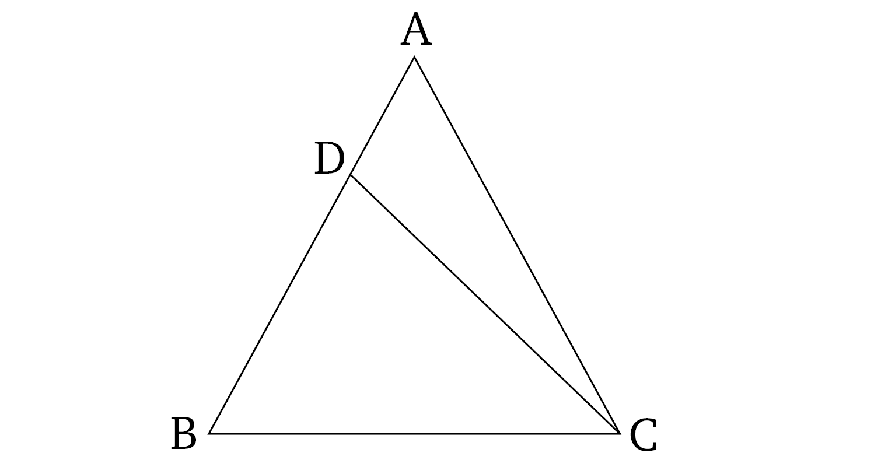
\includegraphics[width=0.55\textwidth]{blaszczyk/bla-fig1a} 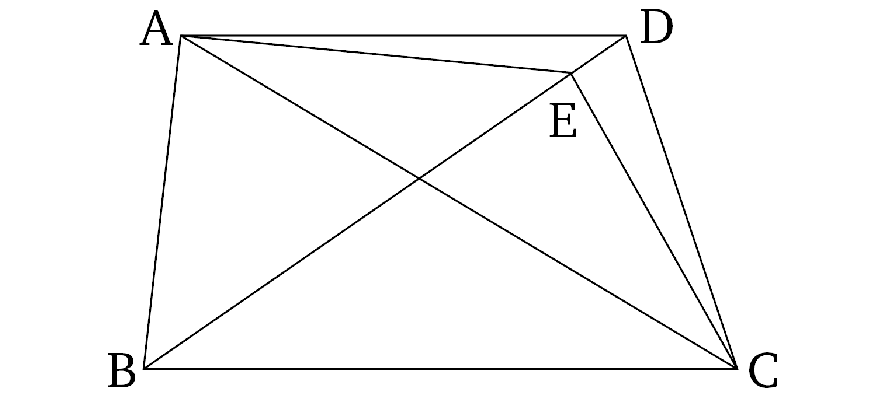
\includegraphics[width=0.55\textwidth]{blaszczyk/bla-fig1b}}
\caption{\textit{Elements}, I.6 (on the left) and 39 (on the right).}
\label{figCN5}
\end{figure}
\subsection{5.2. Mancosu on numerosities}

Paolo Mancosu \parencite*{ref_pm09} is the first study introducing numerosities into a philosophical debate. 
\parencite{ref_pm16} applies numerosities in discussion on the so-called Hume Principle. In what follows, we focus on the former study.


Let start with mathematics. Seeking to present an alternative to Cantor's theory of cardinal numbers, Mancosu adopts labeled sets version, takes $\ell$ to be the identity map, and applies numerosities to subsets of $\N$.\footnote{He refers to \parencites{ref_BN03}{ref_BN06}{ref_BN07} and some other papers. For obvious reasons, he could not refer  to \parencite{ref_BN19}.}

He obtains the extension of natural numbers to hypernatural numbers \mbox{$(\N^*,+\cdot,0,1,<)$} through the ultrapower construction. However, to this end,  following Benci, he applies a selective ultafilter.\footnote{The existence of selective ultrafilters follows from the Continuum Hypotheses. There are models of ZFC with no such filters \parencite[see][76]{ref_tj}} 
Despite involving such strong means, results are a bit below the ones presented in section \S\,4.1 above. 


Mancosu determines numerosity of $\N$ in the same way as we did in section \S\,4.1. So, let us adopt the same notation, $numerosity(\N)=\alpha$. Results regarding odd and even numbers are similar to those presented in section \S\,4.1 above. 
 
 Numerosities of sets $\{kn:n\in\N\}$ and $\{n^2:n\in\N\}$ equal  to  $\alpha/k$, $\sqrt{\alpha}$ respectively. Yet,  it is up to a reader to check why these hyperreal numbers belong to $\N^*$.  In the historical part of the paper, Mancosu discusses Galileo's paradox, yet in the mathematical part, he does not justify the inequality $\sqrt{\alpha}<\alpha$.
 Finally, the paper does not show the numerosity version of Euclid's axiom CN5: $numeosity (A)<numerosity(B)$, given $A\subsetneq B$, although it refers to the part-whole axiom
 in the abstract. 
 
 Determining numerosities, Mancosu  applies the \textit{natural order} of natural 
 numbers.\footnote{See $A_n=\{a : l_A(a)\leq n\}$ \parencite[632]{ref_pm09}}
 Therefore, Cantor's ordinal rather than cardinal numbers provide  more accurate counterpart for numerosities. 
When discussing G\"{o}del \parencite*{ref_kg47}, he observes: ``G\"{o}del's reflection aims at showing that in generalizing the notion of number from the finite to infinite one inevitably ends up with the Cantorian notion of cardinal number'' \parencite[638]{ref_pm09}. Indeed, that was G\"{o}del's observation. In the same paper, he refers to ordinal numbers, yet, do not find them as extending finite numbers.  However, one can extend the structure of finite numbers, $(\N,+,\cdot, 0,1,<)$,  to cardinal or ordinal numbers. Regarding ordinal numbers, the alternative has been discovered already at the beginning of the 20\textsuperscript{th} century by Gerhard Hessenberg \parencite*{ref_gh06} and his definition of normal sums and products.\footnote{In \parencite[\S\,8]{ref_bf},  we show embedding of ordinal numbers with normal sums and products into the field ONAG.} And indeed, founders of the numerosity project refer to the structure of ordinal numbers with normal sums and products in numerous papers.
 

\subsection{5.3. Mancosu on infinite numbers in a historical context}

The substantial part of \parencite{ref_pm09} consists of a historical survey on mathematical infinity. It is a must-read study for anyone interested in the history of mathematics.  Here, we mention only two issues, which Mancosu omits (maybe intentionally). The first is the tradition of geometrical optics from Euclid to Descartes. In short, it was a dogma of the 17\textsuperscript{th}-century optics that light propagates with infinite velocity. Still, it differed depending on the medium of propagation. 
Consequently, there
was a scale of infinite velocities. Although Descartes faultily believed that light propagates
faster in water or glass than in air, he could establish the ratio of these two
infinities to derive the law of refraction \parencite[see][]{ref_pb20}.

The second issue concerns Cantor's arguments against infinitesimals. Mancosu touches that point regarding Cantor-Bolzano debate. Yet it was Cantor's proxy dispute with Euler and his idea that infinite numbers are inverses of infinitesimals. 
All through his mathematical career, Cantor sought to prove the inconsistency of infinitesimals. Euler in his \textit{Introductio in Analysin Infinitorum} \parencite*{ref_LE48}---the most important treaty in the history of mathematics --
applies both infinitesimals and infinite numbers. Strangely enough, there are only a few references to \parencite{ref_LE48}, of minor importance, in Cantor's papers and letters. 
That bare fact is more significant than Cantor's explicit comments on alternative theories of infinite numbers \parencite[see][]{ref_bf}.

\paragraph{Acknowledgments}
The author is supported by the Polish National Science Centre grant 2018/31/B/HS1/03896.


\end{artengenv}




\addtocontents{toc}{\protect\pagebreak}



\sekcja{Z prac Komisji Filozofii Nauk PAU}{Proceedings of the PAU Commission\\\ on the Philosophy of Science}

\begin{artengenv}{Wojciech Grygiel}
	{Cognitive aspects of the philosophical and theological coherence of the concept of a~miracle within the contemporary scientific world view}
	{Cognitive aspects of the philosophical and theological coherence\ldots}
	{Cognitive aspects of the philosophical and theological coherence\\of the concept of a~miracle within the contemporary scientific world\\
	view}
	{Pontifical University of John Paul II in Krakow}
	{The purpose of the article is to investigate the philosophical and theological validity and coherence of the classical concept of a~miracle within the contemporary scientific world view. The main tool in this process will be the cognitive standard model of the formation of religious beliefs operative in the cognitive science of religion. The application of %
	this model shows why an intentional agent is assigned as responsible for the occurrence of events with no visible cause such as a~miracle: miracles are events that violate the intuitively expected behaviors observable in the physical reality. It will become evident that much of the conceptual content of the classical understanding of miracles can be retained despite of the ontological and epistemological challenges of the contemporary science. In particular, this concerns the semantic view of miracles in which a~miracle does not occur as an objective Divine intervention but qualifies as religious interpretation of the natural course of events always in reference to a~cultural and personal context that is unique to those who directly experience these events either as direct recipients or as observers.}
	{miracles, divine action, panentheism, cognitive science, intuition.}
	
	



\section*{Introduction}
Subjecting miracles to a~scientific study may sound like a~violation of the main principle of science, that is, the principle of methodological naturalism. The principle stipulates that science should rely on natural explanations only: nature should be explained by nature
%\label{ref:RNDt4AiRSjYlg}(e.g. Plantinga, 2001).
\parencite[e.g.][]{plantinga_methodological_2001}. %
 Many events commonly considered as miraculous manifest themselves in the physical realm suggesting that natural causes must be at least partially responsible for their occurrence. This is indeed the case when a~purely natural phenomenon is qualified as miraculous without reference to any supernatural agency. It turns out that the common sense classification of a~given phenomenon as miraculous very quickly raises serious concerns as to whether it is something extraordinary indeed or it is just the perception of its observer that prompts him or her to designate it as miraculous. In the English language the term \textit{miracle} clearly stems from the Latin \textit{mirari} which means to wonder. We wonder at things both natural and supernatural: we wonder at the discoveries of science and we wonder when we experience a~sudden healing from a~deadly cancer. In the first case we are astonished at what science can do and in the second case we are astonished at what science (at least for now) cannot do and we rush to explain it as the workings of the supernatural forces.

Miracles play a~decisive role in the Christian fundamental theology for they serve to confirm the divinity of Jesus Christ
%\label{ref:RNDWeJfFVcw2K}(Rusecki, 2006, pp.330–359).
\parencite[][pp.330–359]{rusecki_traktat_2006}. %
 Only God can heal the sick and raise from the dead. Miracles are also taken into account in the processes of beatification and canonization of confessors, that is, individuals that gave witness to the faith by the way they lived. A~miracle must occur through the intercession of a~candidate whereby God is believed to grant a~sign that he or she is enjoying the glory of heaven by performing a~miracle for which he or she interceded 
%\label{ref:RNDR85eQQSTKN}(John Paul II, 1983).
\parencite[][]{john_paul_ii_apostolic_1983}. %
 At this point a~fundamental question arises: if the progress of science reveals that certain diseases can be cured by purely natural means, does this invalidate the approved beatifications and canonizations? Worse yet, does this undermine the divinity of Christ as related by the gospels? The credibility of miracles has been challenged on the scientific grounds by in the 18\textsuperscript{th} century by David Hume who claimed the impossibility of their occurrence due to the inductive character of the laws of nature as exemplified by the Newtonian mechanics 
%\label{ref:RNDfxOdcfEQjo}(Hume, 2008, pp.79–95).
\parencite[][pp.79–95]{hume_enquiry_2008}.%
 The nature and the credibility of miracles remains a~topic of vivid discussions until the present day 
%\label{ref:RNDjupXhPwfba}(e.g. McGrew, 2019).
\parencite[e.g.][]{mcgrew_miracles_2019}.%


The inquiry carried out in this paper involves the application of the cognitive standard model of the formation of religious beliefs to establish the degree to what the classical philosophical and theological understanding of miracles retains its coherence and validity within the contemporary scientific world view. The task is conceptually complex for it hinges upon the understanding of one of the key issues in the contemporary natural theology, namely, that of the mechanism of the Divine action in the Universe
%\label{ref:RNDxt2AO6wyec}(e.g. Murphy, 1995; Słomka, 2021).
\parencites[e.g.][]{russell_divine_1995}[][]{slomka_gods_2021}. %
 The cognitive mechanisms that assign an intentional agent as responsible for the occurrence of events with no visible cause will allow to view miracles as events that violate the intuitively expected behaviors observable in the physical reality. This approach has been already implemented by De Cruz and De Smedt 
%\label{ref:RNDKLAJvbuymi}(De Cruz and De Smedt, 2015, pp.155–178)
\parencite[][pp.155–178]{de_cruz_natural_2015} %
 and the investigative efforts related in this paper take this approach as their point of departure. The task will be carried out in the following steps. Firstly, the classical philosophical and theological significance of miracles will be summarized with the particular emphasis on how hidden causes are invoked to explain these events. Secondly, the cognitive standard model of the formation of religious beliefs will be briefly introduced with the justification in what sense it pertains to the study of miraculous events. Thirdly, the specificity of the dynamics of the scientific growth will be surveyed in to see how the cognitive mechanisms may respond to the events that fall outside of the current knowledge of the nature’s trajectories. Fourthly and lastly, it will be shown how the standard model of the formation of religious beliefs secures many of the components of the classical concept of miracles in a~theological perspective that is consistent with the scientific world view. This coherence is achieved within the semantic view of miracles in which a~miracle does not occur as an objective Divine intervention but qualifies as religious interpretation of the natural course of events always in reference to a~cultural and personal context that is unique to those who directly experience these events either as direct recipients or as observers.

\section*{Miracles classically}
Miraculous events have been reported to occur since times immemorial both in religious and non-religious contexts. The attempts to unveil their nature have been undertaken by many philosophers, theologians and scientists in the entire history of the human intellectual endeavors
%\label{ref:RNDGgRl28nlOY}(e.g. Basinger, 2018).
\parencite[e.g.][]{basinger_miracles_2018}. %
 The contemporary understanding of what event qualifies as miraculous draws from two main classical sources: (1)~the religious thinking of medieval Christian philosophers such as St. Augustine and St. Thomas Aquinas and (2) the modern approach that rests largely on the critical works of David Hume. The major difference in these two sources stems from a~different concept of the fundamental ontology of nature that they assume. While the medieval view relied the ontology of things as individual substances, following the onset of the scientific method in the 17\textsuperscript{th} century the modern view shifted to see the fabric of the Universe as ordered by a~set of physical laws governing its dynamics. What remained intact of the medieval view, however, are the two distinct approaches to miraculous events with Augustine stressing the \textit{semantic} (subjective) and Aquinas the \textit{ontological} (objective) character of miracles.

As Rusecki points out, the works of Augustine impact the understanding of the nature and significance of miracles in all generations of thinkers to come
%\label{ref:RNDd2U3YsBIgH}(Rusecki, 2006, pp.35–36).
\parencite[][pp.35–36]{rusecki_traktat_2006}. %
 Augustine has not only dealt at length with ontological, epistemological and theological aspects of miracles but he has also developed his own view on how these aspects interplay in a~miraculous event. Rusecki argues that Augustine’s approach to miracles emphasizes their theological meaning, namely, that their function is primarily \textit{symbolic} to communicate the Divine plan of salvation of mankind and to strengthen its credibility. Consequently, miracles can be properly interpreted when considered in the religious context. A~detailed analysis of what is implied by the religious meaning of miracles is offered by Świeżyński 
%\label{ref:RNDxQidJQrVKK}(2012, pp.225–273).
\parencite*[][pp.225–273]{swiezynski_filozofia_2012}. %
 Augustine opines that since it is the will of God to maintain in existence all that He has created, God would never act contrary to nature. If miracles seem contrary to nature, it is due to the lack of knowledge of its laws 
%\label{ref:RNDXQPRm4qARv}(Augustine, 2003, \textit{The City of God}, XXI.8).
\parencite[][\textit{The City of God}, XXI.8]{augustine_city_2003}. %
 One of the most famous statements of Augustine concerning miracles, however, is voiced when he claims that the events considered as miraculous do not have to be any more exceptional than all other phenomena because all nature is a~great miracle in itself 
%\label{ref:RNDy8DYiAWkn3}(Augustine, 2003, \textit{The City of God}, X.12; X.16-18; XXI.7; XXI.8).
\parencite[][\textit{The City of God}, X.12; X.16-18; XXI.7; XXI.8]{augustine_city_2003}. %
 The reason some events are perceived as miraculous by the human mind is that they occur \textit{rarely} and as such they attract more attention and cause \textit{astonishment}. In a~strictly ontological sense all that occurs in the Universe according to the laws of nature deserves to be called miraculous because it precisely follows the order instituted by God and it is God Himself who acts in all that takes place in nature. According to Augustine miracles bear primarily epistemological (subjective) character for they arise on the grounds of the lack of the proper knowledge of nature and they acquire their due significance when they are interpreted in the domain of religion.

In contradistinction to the Augustinian conception of miracles were the emphasis falls on the experience of their recipient or observer, the approach adopted by Aquinas focuses on the objective properties of a~miraculous event. He starts out with the consideration of the specificity of the natural order to establish domains of possible phenomena reserved to the Divine action only. In this regard Aquinas clearly implements the Aristotelian methodology which commences from the things natural and based on a~chain of inferences arrives at the knowledge of the things pertaining to God. Aquinas’ understanding of the natural order relies the Aristotelian ontology of substances and represents the totality of the common sense knowledge of the nature of things available to a~scientist of the day before the onset of the contemporary scientific method. The precise meaning of Aquinas’ concept of the natural order has been succinctly summarized by Etienne Gilson
%\label{ref:RND9M2nUbHp3l}(1991, pp.376–377).
\parencite*[][pp.376–377]{gilson_spirit_1991}. %
 Gilson brings up the scholastic understanding of the Divine action in the world by means of the \textit{primary} and \textit{secondary causes}. Since the natural order as the network of the secondary causes is instituted by the act of the free will of God, He can always bypass the workings of the secondary causes and produce the desired effect directly by His power as the primary cause. In light of this, the following statement of Aquinas on miracles acquires its proper precision:

\myquote{
A~miracle properly so called is when something is done outside the order of nature. But it is not enough for a~miracle if something is done outside the order of any particular nature; for otherwise anyone would perform a~miracle by throwing a~stone upwards, as such a~thing is outside the order of the stone’s nature. So for a~miracle is required that it be against the order of the whole created nature. But God alone can do this, because, whatever an angel or any other creature does by its own power, is according to the order of created nature; and thus it is not a~miracle. Hence God alone can work miracles
%\label{ref:RNDAmS1NWBpzc}(Aquinas, 1981, \textit{Summa Theologiae} I.110.4).
\parencite[][\textit{Summa Theologiae} I.110.4]{aquinas_summa_1981}.%


}
The possibility of causal influences made directly by God outside the whole natural order in effecting a~miracle raises some difficulties thereby making the concept of a~miracle incoherent. In order to connect a~miracle with a~non-natural causation, it is necessary to know the boundaries of the natural order. Otherwise, the qualification of an event as a~miracle is ambiguous. Taking into account that the knowledge of the Universe in the 13\textsuperscript{th} century was confined to what was directly observable with a~naked eye and that the Universe in itself was regarded as a~static entity, it seems rational to assume that Aquinas could regard the Universe thus conceived as all that exist in the domain of nature. Moreover, the metaphysical principles derived by Aquinas as he modified those proposed by Aristotle provided the exhaustive explanation of the structure of the Universe and its relation to God whereby all that exists qualifies as the totality of the contingent order of being. Any operation that bypasses the natural order must have God alone as its cause.

It is evident from the above that what Aquinas calls a~miracle is a~sensually detectable event that lies outside the causal capacity of nature and its natural cause is unknown. In addition to this, Aquinas distinguished three degrees of a~miracle depending how far it is removed from the capacity of nature. They may totally exceed the power of nature but they may also engage the natural laws in a~manner that is inaccessible to the natural powers. These degrees are: \textit{supra naturam}, \textit{contra naturam} and \textit{praeter naturam}
%\label{ref:RNDJ5MZ0E98lK}(Aquinas, 1952, \textit{De Potentia Dei}, 6.2.3).
\parencite[][]{aquinas_power_1952}. %
 What seems most apparent from this account is that Aquinas admits of the objectivity of a~miracle, that is, it involves the direct activity of agents who are capable of exceeding the powers of nature and producing effects that could never occur naturally. It is not surprising that Aquinas points to God as the primary cause of miracles for God remains invisible in whatever He does.

In his \textit{Summa Contra Gentiles}, however, Aquinas introduces yet another qualification of a~miraculous event bearing a~more subjective character and referring directly to the etymology of the term \textit{miracle}, namely that of admiration and astonishment. Aquinas writes:

\myquote{
Things that are at times divinely accomplished, apart from the generally established order in things, are customarily called miracles; for we admire with some astonishment a~certain event when we observe the effect but do not know its cause. And since one and the same cause is at times known to some people and unknown to others, the result is that of several who see an effect at the same time, some are moved to admiring astonishment, while others are not. For instance, the astronomer is not astonished when he sees an eclipse of the sun, for he knows its cause, but the person who is ignorant of this science must be amazed, for he ignores the cause. And so, a~certain event is wondrous to one person, but not so to another. So, a~thing that has a~completely hidden cause is wondrous in an unqualified way, and this the name, miracle, suggests; namely, what is of itself filled with admirable wonder, not simply in relation to one person or another. Now, absolutely speaking, the cause hidden from every man is God
%\label{ref:RNDs2oHP9DjvD}(Aquinas, 1975, \textit{Summa Contra Gentiles}, III.101).
\parencite[][\textit{Summa Contra Gentiles}, III.101]{aquinas_summa_1975}.%


}
In this passage Aquinas supplements his treatment of miracles reported above by adverting not to the objective properties of such events but to the subjective response of the recipient or the observer. Unlike Augustine who ties the astonishment with the rarity of a~given event, Aquinas maintains that the astonishment takes place when the cause of event is unknown. An event that qualifies as miraculous only if this astonishment cannot be overcome by any future growth of the knowledge of the workings of the Universe. Aquinas concludes that these events have hidden causes in an absolute sense and only God can be such a~cause. Similarly to what has been addressed above, the proper discrimination of what may lead to a~surprise in an unqualified way calls for the exact knowledge of the boundaries of the natural order. Although these boundaries could have been intuitively clear within the pre-scientific world view, Aquinas’ understanding of miracles loses its coherence within the context of the contemporary science due to the constant expansion of what falls under the description of the scientific theories.

Although Aquinas admits that some natural causes may also remain hidden, the main force of his argument rests on considering God as totally imperceptible by the human sensation. With this being undeniably true, what seems surprising is that Aquinas strangely downplays the immanence of God in the contingent order in his treatment of miracles. It does not quite square with his metaphysics in which he treats every contingent being (\textit{ens}) as a~composite of \textit{esse} and \textit{essence}
%\label{ref:RNDYZ1p5pfEC6}(Aquinas, 1968).
\parencite[][]{aquinas_being_1968}. %
 Since the act of \textit{esse} is that by which God calls things into being and maintains them in existence, by this very act He makes Himself intimately present in creation. In his \textit{Summa Theologica} Aquinas clearly tied the Divine immanence to creatures’ existing by stating: `` \ldots a~thing’s existence is more interior and deep than anything else \ldots and hence it is necessary for God to exist in all things, and intimately so'' 
%\label{ref:RNDWFXxD4gqBz}(Aquinas, 1981, \textit{Summa Theologica}, I.8.1).
\parencite[][\textit{Summa Theologica}, I.8.1]{aquinas_summa_1981}. %
 In other words, the reason why anything whose existing is not its defining essence derives from and depends for its existence on the Creator. As a~result, there is profound closeness between creature as effect and Creator as the cause in this dependence. God is immanent in the natural order.

A~marked shift in the understanding of the nature of miraculous events occurred with the onset of the scientific method in the 17\textsuperscript{th} century when the fabric of the Universe ceased to be perceived substantially in favor of this fabric taking a~form of a~mathematical structure of the laws of nature. Contrary to the position of Aquinas where God would supplement the workings of nature with His direct intervention, the only possibility for God to act beyond nature is to expressly violate its laws. In such case miracles mean exceptional events that disrupt the uniformity of nature. According to David Hume, the scientific laws are discovered inductively based on repeated observations of regularities in nature indicating that the events observed occur with high probability due to the deterministic course that these events take. Since according to Hume miracles are rare events, that is, they have low probability, their empirical evidence can never outweigh the evidence of inductively accumulated data in support of the nature’s routine trajectories
%\label{ref:RNDjSnMuPU4Ii}(Hume, 2008, pp.79–95).
\parencite[][pp.79–95]{hume_enquiry_2008}. %
 Consequently, the violation of the laws of nature cannot not be established with certitude proper to the scientific method and miraculous events lack their credibility. De Cruz and De Smedt argue that such conceptualization of miracles is incoherent because if they occurred with higher probability, ``they would not be violating an established law of nature in the first place'' 
%\label{ref:RNDfsW7HT4T6e}(De Cruz and De Smedt, 2015, p.159).
\parencite[][p.159]{de_cruz_natural_2015}.%


\section*{The standard model}
The main purpose of applying the cognitive standard model of the formation of religious beliefs to the study of the miraculous events is to show why the human mind intuitively places an intentional agency as the cause of an event when its direct physical cause remains hidden. It turns out that the human mind has a~marked conceptual bias resulting in the content – specific cognition that makes the human mind handle different kinds of information with different weight
%\label{ref:RNDf8THkrOgwP}(Barrett, 2011, pp.35–39).
\parencite[][pp.35–39]{barrett_cognitive_2011}. %
 This type of cognition favors a~set of intuitive expectations on the nature of the world and what course of the natural phenomena is most probable. These expectations combine to what is designated as the \textit{folk ontology} 
%\label{ref:RNDkBjb7tiE0E}(e.g. Barrett, 2011, pp.58–95).
\parencite[e.g.][pp.58–95]{barrett_cognitive_2011}. %
 Since folk ontology amounts to the adaptively and developmentally acquired common sense knowledge of the Universe without the aid of the contemporary scientific method it may be to a~reasonable approximation viewed as coinciding with what constitutes the natural order according to Aquinas.

Pascal Boyer proposed that the religious beliefs feed predominantly on the intuitive (non-reflective) concepts to make these beliefs operative in the real-time activity
%\label{ref:RNDj0jiLjvhFh}(Boyer, 1994, 2001).
\parencite[][]{boyer_religion_2001}. %
 Also, he argued that the quickly disseminating religious concepts are those that reach beyond the folk ontology only to a~small degree. These concepts were subsequently named as \textit{minimally counterintuitive} (MCI) 
%\label{ref:RND7xQkMhKiEG}(Barrett, 2000).
\parencite[][]{barrett_exploring_2000}. %
 Minimal counterintuitivity means that only a~few beliefs of the entire intuitive conceptual equipment would not be satisfied thereby making a~given concept or event attractive and astonishing while with other intuitions unchallenged the concept or event in hand would be easily remembered and disseminated. Moreover, these concepts must have sufficient \textit{inferential potential} to produce reflective beliefs necessary to make sense of what is being observed and experienced in reality. It turns out the minimally counterintuitive intentional agents equipped with mental states are employed by the human mind as the principal meaning making tools. And, most importantly from the point of view of this study, De Cruz and De Smedt 
%\label{ref:RNDiJwT2xgVuZ}(2015, pp.161–165)
\parencite*[][pp.161–165]{de_cruz_natural_2015} %
 argue that miracles and the accounts of their stories qualify as the MCI events.

The reason why the human mind interprets natural events with no visible cause as the workings of intentional agents flows from two basic cognitive mechanisms. The first mechanism was originally suggested by Stephen Guthrie and its main task is to over-interpret a~self-perpelled motion as caused by an intentional agent equipped with mental states
%\label{ref:RNDVUX2puV7KX}(Guthrie, 1993).
\parencite[][]{guthrie_faces_1993}. %
 Barrett 
%\label{ref:RNDTmthp1Kbs6}(2000)
\parencite*[][]{barrett_exploring_2000} %
 termed this mechanism as the \textit{hyperactive agency detection device} (HADD). Since such a~motion cannot be explained as the action of a~visible mechanical cause, it does not satisfy the expectation of physicality whereby it activates the HADD so that the assault of a~predator can be prevented and chances for the reproductive success maintained. The second mechanism, namely the \textit{theory of mind} (ToM) otherwise called the \textit{folk psychology}, complements the workings of the HADD by positing mental states and processes that might have led to the predatory behaviors 
%\label{ref:RND8Swxjac1Er}(e.g. Barrett, 2011, pp.74–77).
\parencite[e.g.][pp.74–77]{barrett_cognitive_2011}. %
 This set of ideas combines into what in the cognitive science of religion is termed as \textit{the standard model of the formation of religious beliefs} 
%\label{ref:RNDY42Qvp7S2V}(Murray and Goldberg, 2010, pp.183–189).
\parencite[][pp.183–189]{murray_evolutionary_2010}. %


\section*{Counterintuitivity relativised}
The static Aristotelian Universe studied with qualitative pre-scientific methods had rather little place for surprise and unexpected discovery thereby assuring the relative stability and credibility of intuitions proper to the folk ontology. Contrary to this, however, the development of contemporary science results in a~dynamically changing picture of the world which gradually moves away from these intuitions towards pictures of more generalized and abstract character. The key question at this point is how the human mind responds to this development in its formation of beliefs on the causal activity of intentional agents. In his analysis on what happens as the human mind comprehends the outcomes of the theory of evolution Barrett pointed to two constituents of this response. Taking into account that the complexity of life in the Universe is now known to be the effect of the workings of the Darwinian law of natural selection and not a~purposeful activity of an intelligent designer Barrett asserts that ``we do not simply outgrow the tendency to see the purpose in the world but have to learn to override it''
%\label{ref:RNDCdyeHOl4EK}(Barrett, 2011, p.71).
\parencite[][p.71]{barrett_cognitive_2011}. %
 He comes to this conclusion based on the evidence of empirical studies showing that in this instance the folk ontology intuitions are not easily erased even in the conditions of the high level of scientific literacy 
%\label{ref:RND8GDICmL7C8}(e.g. Casler and Kelemen, 2008).
\parencite[e.g.][]{casler_developmental_2008}.%


A~somewhat different scenario was indicated by Grygiel
%\label{ref:RNDfdn9uA0397}(2020)
\parencite*[][]{grygiel_doctrine_2020} %
 who focused on the concept of a~field which is one of the most brilliant ideas of the contemporary physics. The picture of reality based on physical fields challenges the intuitive belief proper to the folk ontology that motion occurs through contact with a~visible cause. Since fields mediate the action of forces over the entire space in an invisible manner, their effects are perceived as having a~hidden cause. This means that while for the pre-scientific generations events such as moving iron strips with a~magnet could be interpreted as resulting from the action of an intentional agency and quickly acquire religious significance, this is no longer the case for those who are acquainted with the scientific world view based on the notion of the field as a~fundamental theoretical object. On this view, a~ringing cell phone is neither surprising nor an intentional agency is posited to explain the activation of the phone. It is the electromagnetic field of the cell phone network that causes it to ring and this event is no longer counterintuitive. The folk ontology seems to be in much greater recess in this instance as compared to a~purposeful designer invoked to account for the complexity of life in the Universe. This conclusion agrees with the findings of De Cruz and De Smedt 
%\label{ref:RNDJRHZhYVet6}(2012)
\parencite*[][]{de_cruz_evolved_2012} %
 who show the cognitive biases can be offset by the growth of the scientific knowledge and its subsequent cultural dissemination.

In order to reflect the dynamic growth of the scientific knowledge and its influence on the formation of religious beliefs, Grygiel introduced the concepts of the \textit{vincible} and \textit{invincible counterintuitivity}
%\label{ref:RNDQ2kDT75Fo5}(Grygiel, 2017; see also Van Eyghen, 2020).
\parencites[][]{grygiel_science_2017}[see also][]{van_eyghen_religious_2020}. %
 These concepts are useful in understanding a~boundary situation if counterintuitivity was ultimately overcome upon the formulation of a~scientific theory of everything capable of grasping the full meaning of reality as proposed by Hawking and Mlodinov 
%\label{ref:RND4sZujugWEq}(2010),
\parencite*[][]{hawking_grand_2010}, %
 for instance. It is commonly agreed, however, that such expectations are illusory for both practical and theoretical reasons 
%\label{ref:RNDPujZiFiVUt}(e.g. Heller, 2006).
\parencite[e.g.][]{heller_teorie_2006}. %
 The practical reasons were indicated by Albert Einstein who maintained that science discovers a~very small part of the depth of the physical reality only and most of it is hidden as a~profound mystery 
%\label{ref:RNDQ5wYdhMo27}(Einstein, 1931).
\parencite[][]{einstein_world_1931}. %
 In other worlds, nature conceals enough novelties in her womb to violate the intuitions of many future generations of scientists.

The theoretical reasons were accounted for by Michael Heller as he named three irremovable gaps in knowledge that cannot be covered by the progress science: the \textit{ontological}, the \textit{epistemological} and the \textit{axiological}
%\label{ref:RNDi3vF7dvejy}(Heller, 2003a, pp.142–143).
\parencite[][pp.142–143]{heller_chaos_2003}. %
 The ontological gap refers to the Leibnizian question of why there exists something rather than nothing while the epistemological gap prompts the famous Einsteinian puzzlement with the incomprehensibility of the comprehensibility of the Universe. Since the pertinent answers fall outside the competence of science, the problem of the ultimate origin of the structuring of the Universe will never be scientifically resolved. Grygiel argues that even if traces of the pre-scientific folk ontology were still operative, this only adds to how well human mind is actually protected from conquering all counterintuitivity: should the intuitive conceptual biases be ever overcome and should the folk ontology ever catch up with the actual state of the art in science, it is unlikely that nature itself will ever run out of surprises 
%\label{ref:RNDXwYn3taisJ}(Grygiel, 2017).
\parencite[][]{grygiel_science_2017}.%


Although it seems rational to accept that the folk ontology can be at least tamed or even transformed to some degree following the progress of science, this does not happen in course of simple inductive generalizations of frequently occurring empirical evidence. Rather, transformations of these ontologies take place as a~result of changes in the theoretical description of reality and their subsequent cultural assimilation to form a~scientifically informed world view. According to the well known holistic stance of Willard V.O. Quine, scientific theories themselves can never be abolished by a~single experiment because they constitute a~set of interconnected statements which ``face the tribunal of sense experience not individually but only as a~corporate body''
%\label{ref:RNDrzfHj0dzzj}(Quine, 1951, p.30).
\parencite[][p.30]{Quine1951-QUITDO-3}. %
 Moreover, theories function in conjunction with a~broader context of ``elaborate myths and fictions'' and need experimental agreement along their ``empirical edge'' only 
%\label{ref:RNDRK9jv0dtAY}(Quine, 1951, p.42).
\parencite[][p.42]{Quine1951-QUITDO-3}. %
 This means that the folk ontologies can easily coexist with the contradictory empirical evidence indicating that even frequent events violating the intuitive expectations will generate beliefs that they are caused by hidden intentional agents. Contrary to Hume’s empiricism, these events could still qualify as violating the laws of nature and interpreted as caused by God. Would they still be miracles, though?

The answer to this question must be sought in the classical qualification of miracles as rare events (with low probability) that lead to wonder and astonishment. Placed in the contemporary world of cell phones our medieval ancestors would most likely get used to them ringing without a~visible cause but they would still lack the theoretical basis to understand the physical nature of why these phones activate. Unlike the attribution of the intentional agency as a~cause of the counterintuitive events, wonder and astonishment are of psychological nature and they arise due to the rarity of the events experienced. Certainly, these events must be counterintuitive because intuitions would have no chance of being formed out of what is unusual. It turns out that the connection between the low probability of events and their surprising character comes to the fore in the information theory where the entropy of a~random variable is the average level of surprise or uncertainty in the possible outcomes of the variable. More importantly, however, the HADD mechanism has been also discovered to be sensitive to the traces of the activity of the intentional agencies in the form of highly organized patterns which by their nature exhibit low probability of appearance
%\label{ref:RNDQbM3jtYEds}(Barrett, 2004, pp.36–39; Grygiel, 2020).
\parencites[][pp.36–39]{barrett_why_2004}[][]{grygiel_doctrine_2020}.%


The cognitive considerations carried out in this section throw an interesting light on the coherence of the classical understanding of miracles. Firstly, it can be maintained that miracles are caused by a~hidden intentional agency which is attributed by the HADD mechanism responding to the violation of the intuitive folk ontologies. This in turn does not mean the bypassing or the violation of the constancy of the laws of nature at all and it squares with the ontological views of what constitutes the fundamental fabric of reality consistent with the contemporary science. Furthermore, miraculous events may also remain rare because the HADD mechanism will properly respond to their counterintuitivity and the psychological effect of wonder and astonishment will follow. Astonishingly enough, the application of the standard cognitive model of the formation of religious corroborates the consistency of the key components of the classical understanding of miracles in the context of the contemporary science with a~marked bent towards the Augustinian view where miracles are treated as contrary to nature not because they violate its laws but because these laws remain unknown. The demonstration of further consistency with Augustine calls for a~theological analysis which will be offered in the following section.

\section*{Challenging supernaturality}
It is commonly accepted that the conceptual foundation of the cognitive sciences is quite foreign to that of the classical philosophical discourse
%\label{ref:RNDcRhk8D4F1S}(e.g. Brożek, 2013; Grygiel, 2011).
\parencites[e.g.][]{brozek_philosophy_2013}[][]{grygiel_metodologiczne_2011}. %
 This pertains to the cognitive science of religion as well. It seems surprising, however, that researchers in the area of the cognitive science of religion do not properly address a~certain marked conceptual inconsistency that evidently plagues their inquiries. This concerns the direct match made between \textit{supernatural} and \textit{counterintuitive} 
%\label{ref:RNDodu4f4tug0}(e.g. Barrett, 2011, p.97)
\parencite[e.g.][p.97]{barrett_cognitive_2011} %
 which will lead to a~clear confusion in case when a~purely natural event has no visible cause and is explained by means of the action of an intentional agent. Consequently, the religious interpretation of such events will not discriminate between what is of the natural and what is of the Divine origin. This evident difficulty is a~good starting point to address the last issue regarding the coherence of the classical notion of a~miracle within the context of the contemporary science with the aid of the standard cognitive model of the formation of religious beliefs, namely, that of the Divine action.

The problem of the Divine action involved in the miraculous events within the world view consistent with the contemporary science has been the subject of many vivid discussions and controversies. The main point of contention is whether this world view admits of the so called \textit{special Divine action} which is understood as divine action which reaches beyond creation of the Universe and beyond the ordinary maintaining it by God in its existence. To put things in in short, is whether God can somehow intervene within the network laws that govern the Universe either by violating them or exploiting the loopholes in the causal closure of the Universe. This problem has become the focal point of a~major research project undertaken in the years 1988-2003 by a~large group of scientists, philosophers and theologians and termed by Wildman
%\label{ref:RNDdR6ymgg6uY}(2004)
\parencite*[][]{wildman_divine_2004} %
 as ``The Divine Action Project''. Most of the project’s participants conceded to the idea that the preferred mode of the Divine action in the world is \textit{non-interventionistic} on the grounds that it would be contradictory to hold that on one side God runs the Universe according to its laws and on the other disrupts this order by His interventions 
%\label{ref:RNDnWaW6PekcW}(e.g. Peacocke, 1995; Russell, 2001).
\parencites[e.g.][]{peacocke_gods_1995}[][]{russell_divine_2001}. %
 This stance has been objected to by Plantinga who argues that one can claim compatibility of special divine action by means of interventions in the context of the contemporary scientific theories such as quantum mechanics, for instance 
%\label{ref:RNDCfr6Ae0RRr}(Plantinga, 2008).
\parencite[][]{plantinga_what_2008}. %
 A~prominent representative of this group, an English theoretical physicist and theologian John Polkinghorne 
%\label{ref:RND0Qq2dOOCsa}(1998, p.92),
\parencite*[][p.92]{polkinghorne_science_1998}, %
 asserts the following:

\myquote{
It is theologically incredible that God acts as a~kind of celestial conjurer, doing occasional tricks to astonish people but most of the time not bothering. Such a~capricious notion of divine action is totally unacceptable. The main problem of miracle, from the theological point of view, is how such wholly exceptional events can be reconciled with divine consistency.

}
Moreover, Polkinghorne’s thinking reveals certain closeness to the terminology employed in the cognitive science of religion as suggest the use of the concept of \textit{regime}, that is the domain of experience, in which the human mind is accustomed to a~certain course of natural events. This is a~close match of the \textit{folk ontology}. As an example he introduces the phase changes which can lead to drastic changes of behavior governed by the same physical laws. In other words, these drastic changes are subject to unchangeable physical laws indicating that miracles do not have to imply the violation of these laws. Another suitable example would be the Einstein field equation which for small gravitational forces predicts the flatness of space-time consistent with the folk ontology while for strong gravity induced by large masses it predicts space-time curvature entirely foreign to our common sense perception.

Although Polkinghorne does not dwell on the issue of miracles at length, he makes an interesting observation that leaves a~valuable clue as to how to interpret miracles in the context of the scientific picture of the world. He states that: ``Miracles are not to be interpreted as divine acts against the laws of nature (for these law are themselves expressions of God’s will) but as more profound revelations of the character of the Divine relationship to creation''
%\label{ref:RNDWX77FDc5ZR}(Polkinghorne, 1998, p.93).
\parencite[][p.93]{polkinghorne_science_1998}. %
 In the clearly Augustinian tone Polkinghorne implies here that miracles should not infringe upon the deep harmony that exists between God and His creation and that they should be correlates of the natural course of events. It turns out that according to the methodological reflection on the growth of scientific knowledge that has been already addressed above, a~\textit{non-interventionist} model of the divine action is now preferred 
%\label{ref:RNDeeAImeoP8N}(e.g. Heller, 2002, pp.117–121).
\parencite[e.g.][pp.117–121]{heller_sens_2002}. %
 This model is best articulated in the context of \textit{panentheism}: ``all-in-God'', which is an ontological stance relating the natural and the supernatural orders as the natural realm being immersed in the supernatural 
%\label{ref:RNDHgbFGNrQBY}(e.g. Clayton and Peacocke, 2004).
\parencite[e.g.][]{clayton_whom_2004}.%


The non-intervetnionist model of the Divine action in the world neutralizes the difficulty of the match between the counterintuitive and the supernatural because in this model the immanent God achieves His goals solely through the workings of the laws of nature in which He is constantly present. The non-interventionist model squares well with a~broader set of ideas on the relation of the natural to the supernatural known as panenthesim (``all in God'')
%\label{ref:RNDz10LEmjPyo}(e.g. Peacocke, 2004).
\parencite[e.g.][]{peacocke_articulating_2004}. %
 Since in such circumstances God’s action occurs through the powers of nature only, counterintuitivity pertains exclusively to the events that follow laws unknown to science and not occur due to the divine interventions. This shows remarkable consistence with the Augustinian understanding of miracles as the works of nature itself because in the panentheistic setting all natural events qualify as supernatural since in each instance they reflect the divine causality mediated through the laws of nature. It turns out that the conceptual inadequacy of the division of all that exists into natural and supernatural domains has been pointed out by theologians. For instance, a~prominent German theologian Gisbert Greshake 
%\label{ref:RNDi30mMDj0wf}(1997, p.37)
\parencite*[][p.37]{greshake_dreieine_1997} %
 states:

\myquote{
In fact, there is no such thing as a~purely natural order. What creation is and is called is in fact always that world which was founded in the Son out of the most free love and was created for the Son and his ``\textit{Pleroma}'' (fulness). It is that world in which man was called to life with the triune God. It is the world of which the Prolog to the Gospel of St. John speaks that Logos has always been in it and of which the Old Testament clearly says that the Holy Spirit fills it and works~in~it.

}
Consequently, the acceptance of the stance of panentheism mandates the neutralization of the commonly accepted division of reality into natural and supernatural. The Divine immanence in the created (contingent) order makes everything that happens the work of God and there is not a~bit of reality that lies beyond His constant causal influence. Consequently, Greshake does not hesitate to claim that since according to the Christian doctrine God is triune in His essence, namely the unity of three Divine persons, there arises an urgent need for the Trinitarian ontology, cosmology, anthropology and sociology
%\label{ref:RNDRtgkaCnuBn}(Greshake, 1997, p.42).
\parencite[][p.42]{greshake_dreieine_1997}. %
 Furthermore, the immanence of God in creation can be viewed as manifesting itself as the rationality of the Universe. Inspired by a~Danish historian of science, Olaf Pedersen 
%\label{ref:RNDheNqT8xfAN}(2007, pp.63–65),
\parencite*[][pp.63–65]{pedersen_two_2007}, %
 Heller admits ``that Christ the Logos implies that God’s immanence in the world in its rationality 
%\label{ref:RNDB4VC7za3qG}(Heller, 2003b, p.57).
\parencite[][p.57]{heller_scientific_2003}. %
 As Heller maintains, this rationality can find varying expression in the human thought resulting in that this rationality can assume different ``incarnations''. While the first incarnation of this rationality was the Greek philosophy, its contemporary incarnation is the scientific rationality. Moreover, Heller 
%\label{ref:RND4Fd3MlFypB}(2016)
\parencite*[][]{heller_teologia_2016} %
 stipulates that the scientific rationality is superior to that of the Greeks for it unveils the Logos immanent in nature in a~greater degree.

\section*{Conclusions}
In conclusion of the study it can be asserted that the analysis of the nature of the miraculous events with the use of the standard cognitive model of the formation of religious beliefs reveals that this model comes to great assistance in demonstrating the marked coherence of the classical Augustinian understanding of miracles with the world view supported by the contemporary science. This happens at the expense of the distinction between the natural and supernatural because the immanence of God in nature makes everything that happens in nature directly His work and thus supernatural. Strictly speaking, there is no purely natural order. It is now a~point of controversy whether the cognitive mechanisms responsible for the attribution of an intentional agency to an event with a~hidden cause are error management or truth-tracking tools
%\label{ref:RNDhi3KYAxopq}(Barrett and Church, 2013; Van Eyghen, 2019).
\parencites[][]{barrett_should_2013}[][]{van_eyghen_is_2019}. %
 Their primary role is to prompt the recipient or the observer of a~counterintuitive event to read it as being caused by God and to interpret this event as miraculous. As it has been explained, this process is contextual for the attribution of an intentional agent is relativised to what the one who observes the miracle considers to be consistent with the expectations of the folk ontology he or she is equipped with. When this attribution is made, a~given event immediately acquires religious meaning because God conceptualized as an intentional agent easily combines into most of the religious narratives present in the contemporary culture 
%\label{ref:RNDz8GXAh37pX}(e.g. De Cruz and De Smedt, 2015, pp.172–178).
\parencite[e.g.][pp.172–178]{de_cruz_natural_2015}. %
 Contextuality of miracles thus exercised prevents the invalidation of miracles once the events that are associated with them acquire their natural scientific explanations reaching beyond the content of the folk ontology. In short, canonized saints remain canonized. The semantic reading of miracles remains in accord with the hermeneutical attitudes in the contemporary theology and has become the standard understanding in instances when miracles serve as arguments in favor of the Divine action 
%\label{ref:RNDFfJg1hCAzw}(e.g. Rusecki, 2006, pp.211–290).
\parencite[e.g.][pp.211–290]{rusecki_traktat_2006}. %
 Also, as De Cruz and De Smedt 
%\label{ref:RND5jacUx1XKS}(2015, p.160)
\parencite*[][p.160]{de_cruz_natural_2015} %
 point out, the cognitive support for miracles enhances their credibility because the unusualness of such an event is no longer the matter of an entirely subjective response in line with personal tastes and predilections but is inferred by the natural powers of human cognition.

The very last remark of this study is addressed to the critical mind: is it possible that the apparatus of the cognitive science of religion offers an ultimate proof that by the belief in miracles the human mind is fooled into thinking that some transcendent reality has dominion over the Universe? It turns out the scientific studies of religion using cognitive methods receive a~variety of philosophical interpretations among which those claiming that explaining religion means explaining religion away appear as quite dominant
%\label{ref:RNDivr7veuisS}(e.g. Boyer, 2001, p.76; Pyysiäinen, 2001, pp.78–79).
\parencites[e.g.][p.76]{boyer_religion_2001}[][pp.78–79]{pyysiainen_cognition_2001}. %
 These interpretations attempt at disproving the truthfulness of the religious claims based on the knowledge of the mechanism of their origin. As Murray and Goldberg 
%\label{ref:RND3u9aFJdkad}(2010, pp.193–199)
\parencite*[][pp.193–199]{murray_evolutionary_2010} %
 point out, however, this is but a~typical instance of a~logical error designated as the \textit{genetic fallacy} in which to know how a~given belief is formed is taken as the proof that the belief is true. By the same token one can claim that it would be a~genetic fallacy to discredit the religious meaning of miracles as caused by God just because the origins of this belief were scientifically explained by the tools of the cognitive science of religion. In addition to this Barrett suggests that genetic explanations of religion are in force when one does not believe that God exist only. If he or she does, the knowledge on how they arrived their beliefs serves to better understand their faith 
%\label{ref:RNDg9lWzR7uyD}(Barrett, 2011, pp.148–155; see also Wszołek, 2004, pp.51–54).
\parencites[][pp.148–155]{barrett_cognitive_2011}[see also][pp.51–54]{wszolek_wprowadzenie_2004}.%


\end{artengenv}


\begin{artplenv}{Dominika Oramus}
	{Nowe światy literackie: literaturoznawstwo współczesne a~nauki ścisłe}
	{Nowe światy literackie: literaturoznawstwo współczesne a~nauki\ldots}
	{Nowe światy literackie: literaturoznawstwo współczesne a~nauki\\ścisłe}
	{University of Warsaw}
	{New literary worlds. Contemporary literature studies and science}
	{Since 1959, when C.P. Snow delivered his seminal lecture \textit{The Two Cultures} on the lack of understanding between scholars working in the humanities and their colleagues from science departments, the gap between the two groups has been one of the most notorious clichés of contemporary Western culture. The aim of this article is to show that this seemingly insurmountable abyss between sciences and the humanities that was brought to the forefront during the mid-20\textsuperscript{th} century is slowly receding into history. Literature studies today is heavily indebted to modern science. Biology (especially evolutionary biology), physics (especially quantum physics), and ecology (especially the Anthropocene studies) are among the most important subjects scholars of literature have to take into account. In order to prove this point I~shortly describe literary genres which introduce modern science to the readers: science fiction, cyberpunk, solarpunk, lablit, quantum fiction, and cli-fi. I~also refer to the newly-emerged schools of criticism-science fiction studies, ecocriticism and evocriticism-to show how scholars discuss these texts within the framework of the humanities. Additionally, I~give a~sample discussion of one of the cli-fi's classics, J.G. Ballard’s \textit{The Drowned World} and also shortly discuss two science fiction novels concerned with the civilisational conflict between science and humanities: Stanislaw Lem's \textit{His Master's Voice} and Margaret Atwood's \textit{Oryx and Crake}.}
	{science fiction, climate fiction, quantum fiction, cyberpunk, solarpunk, science versus humanities, anthropocene, James Graham Ballard, Stanisław Lem, Margaret Atwood.}




\lettrine[loversize=0.13,lines=2,lraise=-0.01,nindent=0em,findent=0.2pt]%
{L}{}iteraturoznawstwo pojmowane jako studia nad rozmaitego typu dyskursami pozwala śledzić fascynacje i~obawy związane z~doświadczeniem życia we współczesności oraz nie wyklucza z~badań tekstów kultury odbiegających stylistycznie czy formalnie od wielkich dzieł z~kanonu literatury narodowej ani światowej. Takie poszerzenie literaturoznawczego pola badawczego skutkuje ważnym spostrzeżeniem: współczesna humanistyka jest pod ogromnym wpływem nauk ścisłych. Biologia (zwłaszcza teoria ewolucji) i~ekologia (zwłaszcza teoria antropocenu), fizyka (zwłaszcza kwantowa) to najważniejsze obok rewolucji informatycznej naukowe konteksty życia współczesnych ludzi. Znajdują one odbicie w~powstających od drugiej połowy XX wieku tekstach literackich oraz szkołach krytycznych analizujących te teksty. Poniższy krótki przegląd kilku wybranych podgatunków literackich inspirowanych szeroko pojętym przyrodoznawstwem pokazuje w~miniaturze, w~jaki sposób nauki ścisłe inspirują twórców literatury popularnej i~jak podział na literaturę popularną i~wysoką odchodzi do przeszłości.

\section*{\textit{Science fiction} (sci-fi), cyberpunk, solarpunk}
W~ostatniej dekadzie XX wieku część anglosaskich środowisk akademickich uznało \textit{science fiction} za przedmiot badań godny uwagi. Pod koniec ubiegłego wieku powstała słynna \textit{The Encyclopedia of Science Fiction} Johna Clute’a i~Petera Nichollsa, w~której znajdziemy m.in. hasło ,,Definitions of SF''
%\label{ref:RNDMBMddO8e91}(Clute, Nicholls, 1993, s.~311–314).
\parencite[][s.~311–314]{clute_encyclopedia_1993}. %
 Ukazuje ono, jak w~kolejnych dekadach XX wieku zmieniało się pojmowanie terminu fantastyka naukowa -- co pośrednio pokazuje zmiany recepcji odkryć naukowych w~kulturze popularnej. Kingsley Amis, autor \textit{New Maps of Hell} 
%\label{ref:RNDWDxvVuS5Gt}(1960),
\parencite*[][]{amis_new_1960}, %
 jednej z~pierwszych brytyjskich książek o~tym gatunku twierdzi, że \textit{science fiction} nie może operować ekstrapolacją, a~jej zadaniem nie jest przewidywanie na podstawie już istniejących przesłanek dalszych losów naszej cywilizacji\footnote{“Science Fiction is that class of prose narrative treating of a~situation that could not arise in the world we know, but which is hypothesized on the basis of some innovation in science or technology, or pseudo-technology, whether human or extra-terrestrial in origin'' 
%\label{ref:RNDS0xm7Rj1nn}(Amis, 1960, s.~14).
\parencite[][s.~14]{amis_new_1960}.%
}. Rozdział poświęcony definicji fantastyki naukowej został przetłumaczony na język polski i~ukazał się w~antologii \textit{Spór o~SF}:

\myquote{
\textit{Science fiction} jest klasą narracji prozatorskiej przedstawiającą sytuacje, które nie mogłyby się zdarzyć w~świecie, jaki znamy, ale są hipotetycznie postulowane na podstawie jakiegoś odkrycia naukowego lub technicznego, albo pseudonaukowego lub pseudotechnicznego, pochodzenia ziemskiego lub pozaziemskiego
%\label{ref:RNDq8f8JPiOiw}(Handke i~in., 1989, s.~13).
\parencite[][s.~13]{handke_spor_1989}.%
}

James Gunn -- amerykański nestor \textit{science fiction studies} i~twórca najważniejszych antologii gatunku oraz podwalin teorii go opisujących uważa że:

\myquote{
\textit{Science fiction} jest gałęzią literatury, która zajmuje się opisem wpływu zmian na ludzi mieszkających w~świecie realnym, obserwowanym na tle przeszłości, przyszłości lub też z~odległości. Często opowiada o~zmianach zachodzących w~świecie nauki lub techniki, a~zazwyczaj dotyczy spraw, których znaczenie względne jest większe niż znaczenie jednostki czy społeczeństwa; niebezpieczeństwo często tu zagraża cywilizacji lub całej rasie
%\label{ref:RNDv7QICYxF5c}(Gunn, 1985, s.~9).
\parencite[][s.~9]{gunn_droga_1985}.%
}

Jeden z~najważniejszych brytyjskich pisarzy \textit{science fiction} tworzących w~wieku XX, Brian Aldiss, pojmował \textit{science fiction} niezwykle szeroko:

\myquote{
\textit{Science fiction} jest poszukiwaniem definicji człowieka i~jego miejsca we wszechświecie; definicji, która byłaby zgodna z~zaawansowanym, lecz nieuporządkowanym stanem naszej wiedzy (\textit{science}), zwykle prezentowanym w~formie gotyckiej lub postgotyckiej
%\label{ref:RNDdVL9SKw9xH}(Handke i~in., 1989, s.~19).
\parencite[][s.~19]{handke_spor_1989}.%
}

Definicja ta podkreśla, że to dzięki fantastyce możemy opisać doświadczenie psychiczne, jakim jest życie w~ramach cywilizacji technicznej, która istnieje dzięki nauce tak zaawansowanej, że niezrozumiałej dla pojedynczych ludzi. Myśl Aldissa rozwinęła Judith Merril, propagatorka terminu \textit{speculative fiction}:

\myquote{
SF (\textit{science fiction}, ale także \textit{speculative fiction}) to literatura, której celem jest eksplorowanie i~odkrywanie natury rzeczywistości, człowieka i~kosmosu za pomocą technik takich jak: ekstrapolacja, projekcja, tworzenie analogii oraz pisarskie testowanie hipotez... używam terminu \textit{speculative fiction} aby opisać literaturę wykorzystującą tradycję ,,metody naukowej'' (obserwacje, hipotezy i~eksperymenty), aby stworzyć i~przebadać przybliżenia rzeczywistości, które powstają w~oparciu o~znane wszystkim fakty zmodyfikowane przez wprowadzenie zmian. Zmiany te mogą być tworem wyobraźni lub wynikać z~wynalazków, a~dzięki nim powstaje nowe środowisko, w~którym funkcjonują bohaterowie. To obserwacje ich reakcji i~postrzegania mają odkryć nowe prawdy -- o~wynalazkach, o~bohaterach lub o~jednym i~drugim
%\label{ref:RNDQqwiZSWj7k}(Merril, 1966, s.~35–36, tłum D.O.).
\parencite[][tłum. D.O.]{merril_what_1966}.%
}

Definicja Merril pozwala widzieć fantastykę jako narzędzie poznania współczesnego świata oraz bliskiej przyszłości -- dzięki koncentracji na stechnicyzowanym otoczeniu stwarza swoiste laboratorium wyobraźni, w~którym z~kolei umieszcza bohaterów. Ich w~dużej mierze podświadome reakcje na technologię są treścią utworów. Zarówno Merril, jak i~Aldiss, Gunn oraz Amis to pisarze i~krytycy dwudziestowieczni, sprzed doby Internetu -- rozumieli oni \textit{science fiction} jako platformę dyskusji o~technice w~przyszłości. Rewolucja informatyczna, jaka dokonała się w~chwili wprowadzenia komputerów do życia społecznego sprawiła, że \textit{science fiction} pozwoliło opisywać nową teraźniejszość.

Powstanie Internetu zrewolucjonizowało kulturę, wyobraźnię, rozrywkę, rynek książkowy, styl życia ludzkości -- to w~tym momencie stechnicyzowana przyszłość rodem z~\textit{science fiction} stała się ludzką teraźniejszością. Rozwój technik komputerowych spowodował zdominowanie kultury wizualnej przez narastającą falę obrazów-kopii, których oryginał nie istnieje, gdyż są one wygenerowaną technicznie iluzją. Zajęły one ważne miejsce w~świadomości społecznej i~stały się łatwo rozpoznawalnymi ikonami. Choć nigdy nie istniały fizycznie, jak np. bohaterowie filmów fantastycznych, stanowią element uniwersalnego kodu zrozumiały w~całym cywilizowanym świecie.

Jean Baudrillard określił takie ,,kopie bez oryginału'' jako symulakry
%\label{ref:RNDalZAolCx06}(Baudrillard, 2005),
\parencite[][]{baudrillard_symulakry_2005}, %
 które nie są ograniczone do jednego konkretnego tekstu, filmu czy symulacji komputerowej, krążą w~sieci pomnażając liczbę kopii, odbić i~iluzji\footnote{Rozwój technik filmowych powoduje narastającą falę symulakr: gnomy, smoki i~olbrzymy z~filmów o~Harrym Potterze, cała menażeria fantastycznych istot z~\textit{Władcy Pierścieni} i~wielu innych kasowych przebojów filmowych, zajmują ważne miejsce w~świadomości społecznej. Są łatwo rozpoznawalnymi ikonami i~choć nigdy nie istniały fizycznie, stanowią element uniwersalnego kodu zrozumiały w~całym cywilizowanym świecie. Powstają o~nich gry, produkowane są gadżety, a~na odwiedzanych przez rzesze internautów stronach internetowych ,,zawieszane'' są kolejne fikcje -- obrazkowe lub pisane teksty ,,fan-fic'', czyli fikcji tworzonych przez fanów na motywach ulubionych dzieł filmowych czy literackich. Dla wielu mieszkańców postmodernistycznego krajobrazu symulakry te są prawdziwe -- za ich pośrednictwem komunikują się z~innymi internautami, których fizycznie nigdy nie spotkali i~nie spotkają. W~eseju \textit{Simulacra and Science Fiction} Baudrillard opisuje między innymi fikcję generowaną na wielką skalę (na przykład przez współczesne media) niszcząc materialną ,,prawdę'', którą niby przedstawia. Baudrillard sięga do przykładu opowiadania Borgesa, w~którym wykonana w~skali 1:1 mapa pokryła i~w rezultacie zniszczyła przedstawianą krainę. Żyjemy w~czasach implozji znaczeń; wedle Baudrillarda po czasach ekspansji i~towarzyszących jej romantycznych wizji heroicznego podboju kosmosu (w rodzaju \textit{Kronik marsjańskich} Raya Bradbury’ego) nadszedł czas cywilizacyjnego zapadania się w~siebie, zamykania oczu i~tworzenia nibyprzestrzeni zaludnionej przez iluzje -- jak w~niekończących się cyklach halucynacji, które przeżywają bohaterowie Philipa K. Dicka lub w~cyberprzestrzeni z~powieści cyberpunkowych.}. Dla wielu mieszkańców postmodernistycznego krajobrazu symulakry te są prawdziwe -- za ich pośrednictwem komunikują się z~innymi internautami, których fizycznie nigdy nie spotkali. Wirtualny świat wymagał stworzenia całego nowego języka do opisania doświadczeń pracy, komunikacji i~rozrywki w~sieci -- i~to właśnie odłam ,,twardej'' (czyli inspirowanej wprost nowymi odkryciami naukowymi) \textit{science fiction} nazwany \textit{cyberpunk} dał współczesnej kulturze aparat pojęciowy, by mówić o~tym całkiem nowym środowisku. Teksty i~filmy cyberpunkowe pokazują bliską przyszłość cywilizacji Zachodu -- społeczeństwa informatycznego, globalnego, gdzie dzięki rozwiniętej technice symulakry zastępują rzeczywistość. Jednocześnie jednak świat ten boryka się z~realnymi skażeniami, epidemiami i~chorobami cywilizacyjnymi.

Znakiem rozpoznawczym cyberpunku są komputery, sieć, Internet, fascynacja współczesną elektroniką, a~zwłaszcza jej gadżetami. Wiele powszechnie używanych dziś słów (rzeczywistość wirtualna -- VR, haker, cyberprzestrzeń, sieć) ma swoje źródło w~tekstach cyberpunkowych. Literatura ta odzwierciedla, ale i~kształtuje rzeczywistość, oddaje wrażenie życia we współczesnym świecie zdominowanym przez Internet i~technologiczne gadżety, symulakry, symulacje i~animacje komputerowe. Cyberpunk jest refleksją nad kulturowymi konsekwencjami powszechnego stosowania bardzo zaawansowanej techniki -- między innymi wiele uwagi poświęca cyborgizacji, zatarciu się różnic między człowiekiem a~maszyną (np. synapsy ludzkiego układu nerwowego kompatybilne z~końcówkami komputera i~chipami). Cyberpunk jest odpowiedzialny za rozpropagowanie terminologii hakerów oraz zainteresowanie ,,stykiem'' człowieka i~maszyny: implantami, VR, domenami internetowymi, AI (sztuczną inteligencją). Wykreował także stereotyp bohatera czasów wielkomiejskiej przyszłości, żyjącego wedle zasad obowiązujących w~skażonej technologicznej dżungli, lecz mimo to posługujących się własnym kodem honorowym.

Cyberpunk był literaturą \textit{science fiction} przełomu mileniów, która dość szybko przekształciła się w~całą gamę podgatunków potomnych -- najsłynniejszą jest steampunk (przeniesienie estetyki cyberpunkowej w~czasy wiktoriańskie), a~najważniejszą z~punktu widzenia wpływu nauk ścisłych na rozwój literatury -- rodzący się dopiero solarpunk.

Steampunk można więc traktować jako nostalgiczną impresję -- przeniesienie cyberpunkowej estetyki w~fabuły rodem z~historii alternatywnej. Jego związek z~naukami ścisłymi jest bardzo nikły -- choć można mówić o~inspiracjach historią techniki. W~takim ujęciu staje się on pokrewny książkom z~podgatunku powieści neowiktoriańskiej. Pisarstwo takie stało się modne w~okresie, gdy Anglia obchodziła stulecie Złotego Jubileuszu królowej Wiktorii i~przedstawia jej czasy z~pewną dozą nostalgii, stosując zazwyczaj postmodernistyczne techniki narracji, z~których najważniejsza to narracja równoległa. W~wielu powieściach neowiktoriańskich dwa plany czasowe, dziewiętnastowieczny i~współczesny przeplatają się -- jest tak np. w~najsłynniejszej z~nich, \textit{Opętaniu} Antonii Susan Byatt, a~zabieg ten występuje również w~powieściach steampunkowych\footnote{O~\textit{steampunku} i~jego związkach z~literaturą wiktoriańską z~jednej, a \textit{cyberpunkiem} z~drugiej strony Piechota pisze w~\textit{Między utopią a~melancholią. W~kręgu nowoczesnej i~ponowoczesnej literatury fantastycznej}
%\label{ref:RNDW7O3HhYJx6}(2015, s.~87–90):
\parencite*[][s.~87–90]{piechota_miedzy_2015}: %
 ,,To specyficzna mutacja cyberpunku, który w~dynamiczny sposób poszerzył swoje oddziaływania na inne pola kultury, jak film, gry komputerowe, a~nawet design. Dwa człony nazwy (\textit{steam} oraz \textit{punk}) stają się wyznacznikami zainteresowań pisarzy tej literatury. \textit{Steam} (z ang. para, energia parowa) odsyła nas do epoki wiktoriańskiej, wykorzystującej w~przemyśle parę mechaniczną. Autorzy spoglądają na XIX-wieczną rzeczywistość z~pewną nostalgią oraz tęsknotą. Drugi człon -- punk -- odwołuje się do tradycji buntu przeciwko establishmentowi oraz wielkim korporacjom. Twórcy \textit{steampunkowi} tęsknią za czasami, w~których kupno określonego produktu jednoznacznie wiązało się z~jego trwałością oraz gwarantowaną jakością''.}.

Solarpunk jest dla niniejszych rozważań znacznie istotniejszy: pod koniec drugiej dekady XXI wieku stał się -- w~swojej odmianie dystopijnej -- główną płaszczyzną dywagacji na temat roli nauk ścisłych w~zagładzie ekologicznej naszej planety. Jednocześnie jednak część utworów solarpunkowych poświęconych jest nie katastrofalnej teraźniejszości, ale lepszej przyszłości. Wpisując się w~tradycję utopijną, ich twórcy starają się pokazać, że mądrze używana zaawansowana nauka (tak inżynieria genetyczna, jak i~fizyka) może pomóc przezwyciężyć kryzys ekologiczny i~dać asumpt do stworzenia cywilizacji przyszłości, której bliskie będą ideały zrównoważenia cywilizacji i~natury. Solarpunk jest nie tylko podgatunkiem literackim czy artystycznym, ale również ruchem społecznym, zrzesza za pośrednictwem domen internetowych młodych ludzi szczerze zaniepokojonych zanieczyszczeniem środowiska i~modelem konsumpcji, który zdominował współczesny świat. Ludzie ci niekiedy piszą blogi, a~niekiedy utwory literackie, upatrując w~tej estetyce i~ideologii szans na lepszą przyszłość. Na jednej z~takich stron czytamy:

\myquote{
Solarpunk to odmiana fikcji spekulatywnej, prąd artystyczny, moda i~ruch społeczny poświęcony odpowiedziom na pytanie ,,jak wyglądać będzie cywilizacja nie niszcząca środowiska i~jak do niej doprowadzić?'' Estetyka solarpunkowa łączy to, co praktyczne, z~tym, co piękne, i~to, co dobrze zaprojektowane, z~tym, co dzikie i~ekologiczne: jasne i~kolorowe z~porządnym i~stonowanym. Solarpunk jest czasem optymistyczny i~utopijny, a~czasem skoncentrowany na trudach walki, by utopię osiągnąć -- nie jest jednak dystopijny. Ponieważ nasz świat gnębią nieszczęścia, potrzeba nam rad, nie ostrzeżeń. Rad jak żyć wygodnie bez korzystania z~paliw kopalnych, jak sprawiedliwie radzić sobie z~niedoborami i~równo dzielić nadwyżki, jak być \textit{fair} dla siebie nawzajem i~planety, na której żyjemy. Solarpunk to wizja przyszłości, przemyślana prowokacja intelektualna i~możliwy do wdrożenia styl życia
%\label{ref:RNDhdbBMjPmlm}(Solarpunk (definicja),
\parencite[][tłum. D.O.]{noauthor_solarpunk_2021}.
}

To dzięki naukom ścisłym społeczności opisywane w~utworach solarpunkowych są w~stanie osiągnąć równowagę, korzystać z~natury tak, by jej nie niszczyć. Zrozumienie zasad funkcjonowania ekosystemów, zaawansowana genetyka, mistrzowskie wykorzystanie sztucznej inteligencji, a~nade wszystko rozwinięta energetyka eksperymentalna zakładająca uzyskiwanie taniej energii z~odnawialnych źródeł to filary utopijnej przyszłości.

\section*{\textit{Climate fiction} (cli-fi), ekokrytyka, evokrytyka}
Solarpunk jest niekiedy postrzegany jako awangardowy i~utopijny odłam cli-fi, czyli powieści o~zmianach klimatu, nowego podgatunku literackiego, który zdefiniował pisarz i~krytyk Dan Bloom. Nazwa ta, choć powstała w~latach 90. ubiegłego stulecia, obejmuje utwory powstające na przestrzeni drugiej połowy XX wieku (część z~nich powstała zanim narodziła się współczesna świadomość ekologiczna, terminy takie jak ,,globalne ocieplenie'' czy antropocen). Bloom twierdzi, że cli-fi (termin utworzony z~pierwszych sylab angielskich słów ,,klimat'' i~,,fikcja'') to gatunek siostrzany powieści katastroficznej i~\textit{science fiction} (nazwa cli-fi utworzona jest na wzór sci-fi). Można mówić o~jego odrębności, gdyż koncentruje się wyłącznie na zmianach klimatu: ich przyczynach, skutkach, naukowych wytłumaczeniach.

Za powieść założycielską tego podgatunku wielu krytyków uważa napisany jeszcze w~latach sześćdziesiątych XX w. \textit{Zatopiony świat} J.G. Ballarda. Jim Clarke w~pierwszym zdaniu eseju ,,Reading Climate Change in J.G. Ballard'' pisze ,,cli-fi powstało zanim jeszcze klimat zaczął się zmieniać''
%\label{ref:RND11lKuQbk33}(Clarke, 2013, s.~7, tłum. D.O.).
\parencite[][tłum. D.O.]{clarke_reading_2013}. %
 Rachele Dini podejmuje temat zmian klimatycznych we wczesnych utworach Ballarda w~artykule ,,‘Resurrected from its Own Sewers’: Waste, Landscape, and the Environment in J.G. Ballard's 1960s Climate Fiction'' 
%\label{ref:RNDyjU37CjeOx}(Dini, 2021).
\parencite[][]{dini_resurrected_2021}. %
 Adrian Tait zaś napisał esej ,,Nature Reclaims Her Own: J.G. Ballard's \textit{The Drowned World}'' 
%\label{ref:RNDbg28YGH4xv}(Tait, 2016)
\parencite[][]{mcgrath_nature_2016}, %
 w~którym przyrównuje fragmenty \textit{Zatopionego świata} do cytatów ze słynnej, napisanej w~tym samym okresie \textit{Cichej wiosny} Rachel Carson oraz całkiem współczesnych biuletynów publikowanych przez Intergovernmental Panel for Climate Change 
%\label{ref:RNDcnU9zHVRle}(Tait, 2016, s.~158).
\parencite[][s.~158]{mcgrath_nature_2016}. %
 Co ciekawe, w~zachowaniu bohaterów tej powieści można zaobserwować psychiczne symptomy charakteryzujące dzisiejszych ludzi cierpiących na depresję klimatyczną, czyli tzw. ,,\textit{eco-anxiety}'' 
%\label{ref:RNDjkGQyqPREd}(Gifford, Gifford, 2016).
\parencite[][]{gifford_largely_2016}.%


\textit{Zatopiony świat} to pozornie konwencjonalna i~prosta historyjka o~globalnej zagładzie i~smutnym losie niedobitków rasy ludzkiej, jednak katastrofa i~jej skutki to tylko pretekst. Seria burz na Słońcu doprowadziła do katastrofalnego ocieplenia Ziemi, roztopione lody zalały wielkie połacie znanych nam dzisiaj lądów, a~wzmożona radiacja doprowadziła do mutacji roślin i~zwierząt. Zmutowane organizmy na kartach książki Ballarda przypominają przedstawicieli pierwotnych gatunków stworzeń z~najdawniejszych geologicznych epok. Stopniowo, wraz ze zmianami klimatu i~linii brzegowych, świat upodabnia się do tego sprzed milionów lat i~cofa się ewolucja świata ożywionego:

\myquote{
Wskutek wzrostu poziomu temperatury, wilgotności i~promieniowania flora i~fauna naszej planety zaczyna przyjmować formy, które występowały na Ziemi, kiedy panowały tu ostatnio takie warunki, czyli mniej więcej w~epoce triasu. [...] Wszędzie występowała ta sama lawina przemian, ciągnąca życie wstecz, w~przeszłość, i~to tak daleko, że tych kilka organizmów złożonych, którym udało się nie stracić równowagi na zboczu metamorfoz, stanowi teraz anomalię. Mam tu na myśli grupkę płazów, ptaki i~człowieka [...] zlekceważyliśmy najważniejszą istotę na naszej planecie
%\label{ref:RNDUbflWU2T0U}(Ballard, 1998, s.~63).
\parencite[][s.~63]{ballard_zatopiony_1998}.%
}

Słowa te wypowiada jeden z~bohaterów, który ma własne teorie na temat regresu rasy ludzkiej. Nie sugeruje on powolnego przekształcania się ludzi w~troglodytów, lecz udowadnia, że ludzkość stała się anachronizmem, gdyż zmuszona jest żyć w~epoce znacznie wcześniejszej niż jej właściwy biologiczny czas. Wierzy także, że mimo ludzkiej psychiki i~anatomii naczelnych gdzieś głęboko na poziomie komórek zachowaliśmy wspomnienia z~najwcześniejszych etapów ewolucji. ,,Pamiętamy'' naszych prymitywnych przodków. Ta tendencja do ruchu wstecz jest wrodzona, głęboko w~duszy pozostały ślady przejścia od jednokomórkowców do \textit{Homo sapiens sapiens}. W~teorii tej pobrzmiewają freudowskie echa:

\myquote{
Pomyśl jak często większość z~nas miewa ostatnio poczucie \textit{déjà vu}, poczucie, że wszystko to już kiedyś widzieliśmy, a~nawet że aż za dobrze pamiętamy te bagna i~laguny. […] Wszędzie w~przyrodzie widać dowody na istnienie wrodzonych mechanizmów, wyzwalających siły, które spoczywały w~uśpieniu przez tysiące pokoleń, lecz których moc pozostała do dziś nie naruszona
%\label{ref:RNDVD84PP0Ypw}(Ballard, 1998, s.~65).
\parencite[][s.~65]{ballard_zatopiony_1998}.%
}

Bohaterowie Ballarda są wyobcowani i~zamknięci w~sobie -- nie są w~stanie myśleć o~przeszłości i~dojrzeć teraźniejszość. Najlepszą definicję dziwnego szaleństwa, jakie ich ogarnia, daje wymyślona przez Ballarda nowa nauka, neuronika:

\myquote{
Jeśli chcesz, możesz to sobie nazwać Psychologią Totalnych Ekwiwalentów albo krótko: neuroniką, i~odrzucić ją jako metabiologiczne urojenie. Ja jednak jestem przekonany, że tak jak posuwamy się w~przeszłość w~czasie geograficznym, tak wkraczamy również w~korytarz owodni, cofając się w~rdzeniowym i~archeopsychicznym czasie, przypominając sobie podświadomie krajobrazy minionych epok, ich rzeźbę geologiczną i~im tylko właściwą faunę i~florę, tak nam znajomą, jak podróżnikowi korzystającemu z~Wellsowskiego wehikułu czasu
%\label{ref:RND0MxYkuhiHK}(Ballard, 1998, s.~67).
\parencite[][s.~67]{ballard_zatopiony_1998}.%
}

Chociaż bohaterowie Ballarda żartują z~psychoanalizy, wyśmiewają myśl, że rzeczywistość zaczyna przypominać test Rorschacha, \textit{Zatopiony świat} nosi wyraźne wpływy freudowskiej teorii dominacji popędu śmierci nad zasadą przyjemności, Thanatosa nad Erosem. W~późnym eseju \textit{Poza zasadą przyjemności}
%\label{ref:RNDhPXIaCiL7C}(Freud, 1994)
 %tłum. pol. 1994
Freud 
\parencite*[][]{freud_poza_1994} %
odwołuje swoje wcześniejsze twierdzenie, że seksualność i~instynkt samozachowawczy to podstawowe i~biologicznie najstarsze siły. Przyznaje, że teoria zasady przyjemności i~zasady rzeczywistości, które wzajemnie się modyfikują by zapewnić nam maksimum satysfakcji, a~jednocześnie ustrzec nas przed zgubnymi skutkami folgowania wszelkim popędom, nie tłumaczy w~pełni zachowań ludzkich. Instynktowne potrzeby kochania, rozmnażania się i~samoobrony są powierzchowne i~ewolucyjnie najmłodsze, pod nimi ukryty jest prastary instynkt śmierci pchający rasę ludzką ku samozagładzie.

Powyższe odczytanie \textit{Zatopionego świata} pozwala zrozumieć, czemu powieść ta, pół wieku po pierwszym wydaniu, została uznana za klasyczny tekst cli-fi. Ballard opisuje stany psychiczne bliskie odkryciom współczesnych badaczy ,,\textit{eco-anxiety}''. Paul Huebener, którego książki opisują kryzys ekologiczny i~jego echa we współczesnej kulturze, zwraca uwagę na fakt, że depresja klimatyczna pojawia się wtedy, gdy ludzie pojmują, iż zmiany klimatu są nieodwracalne i~muszą doprowadzić do zagłady Ziemi
%\label{ref:RNDhWovHARIC7}(Huebener, 2020).
\parencite[][]{huebener_natures_2020}. %
 Bezsilność jaka ich ogarnia sprawia, że są psychicznie nastawieni na najgorsze. W~artykule \textit{A~Visit to the Climate Anxiety Doctor} Stephanne Taylor -- dziennikarka specjalizująca się w~zagadnieniach klimatycznych -- tłumaczy to zjawisko:

\myquote{
Zmiany klimatu wpływają na ludzką psychikę zarówno kiedy przybierają postać gwałtownych, katastrofalnych zjawisk, jak i~długofalowych, stopniowych procesów. Psychologowie odkryli, że kataklizmy skutkują innymi problemami psychicznymi niż zmiany stopniowe. Gwałtowne katastrofy powodują u~ofiar traumę, zmiany stopniowe -- poczucie beznadziejności, fatalizm i~wreszcie depresję. Wszelkie takie zaburzenia psychiczne mają podobne podłoże: strach o~coraz bardziej niepewną przyszłość i~świadomość, że we współczesnym świecie nie podejmuje się odpowiednich kroków, by zmianom zaradzić
%\label{ref:RND5fbW0fL0wi}(Taylor, 2016, tłum. D.O.).
\parencite[][tłum. D.O.]{taylor_visit_2016}.%
}

Taylor zwraca uwagę na podświadomy lęk o~przyszłość i~nagłe ataki paniki i~smutku, jakie odczuwają pacjenci cierpiący na depresję klimatyczną. Mówią oni o~,,nagłym poczuciu dojmującej beznadziejności, jaka opanowuje ich gdy słyszą o~zagładzie raf koralowych''
i~o~,,dziwnym, przemożnym lęku''
%\label{ref:RNDmDxkISCo4C}(Taylor, 2016, tłum. D.O.),
\parencite[][tłum. D.O.]{taylor_visit_2016}, %
 przypominającym stany psychiczne opisywane przez Ballarda. U~ofiar depresji klimatycznej ,,brak jakiejkolwiek nadziei''
% (Hamilton)
\parencite{hamilton_climate_2016}
 sprawia, że zaburzona zostaje percepcja czasu. Michelle Bastian, badaczka tego zjawiska, stwierdza, że: ,,standardowy czas mierzony zegarami nie jest adekwatny w~kontekście zmian klimatu'' 
%\label{ref:RNDEFbUAtIDnL}(Bastian, 2012, s.~39).
\parencite[][s.~39]{bastian_fatally_2012}. %
 W~naszej epoce nie możemy już wyobrażać sobie czasu jako drogi prowadzącej od teraz ku nieskończonej przyszłości, ale raczej stosujemy model odliczania -- ile jeszcze czasu na tej planecie nam zostało.

Cli-fi pokazuje bohaterów zmagających się z~psychicznymi skutkami depresji klimatycznej, przekonanych, że są świadkami ostatnich dni ludzkości na planecie\footnote{,,Widzę analogię do strachu przed zagładą, jaki panował w~latach 50. w~związku z~zagrożeniem wojną atomową. Zwykli ludzie wtedy również odczuwali silny niepokój i~wiedzieli, że jesteśmy zagrożeni anihilacją''
%\label{ref:RNDdtSt3Ufdqe}(Hamilton, 2016),
\parencite[][]{hamilton_climate_2016}, %
 twierdzi Robert Gifford, profesor psychologii z~University of Victoria, a~także członek American Psychological Association. Organizacja ta uznała oficjalnie zagrożenie płynące z~,,już występującego i~prognozowanego na przyszłość wpływu zmian klimatu na psychikę''
% (Hamilton)
\parencite[][]{hamilton_climate_2016}.
 }. Michelle Bastian przypomina w~kontekście zmian klimatycznych ,,zegar zagłady'', stworzony przez naukowców w~roku 1947. Wtedy to użyto ,,powszechnie zrozumiałej konwencji -- północ oznacza koniec czasu'' 
%\label{ref:RND6Nzfef3oPG}(Bastian, 2012, s.~39),
\parencite[][s.~39]{bastian_fatally_2012}, %
 by graficznie unaocznić zagrożenie wojną atomową. Bastian zwraca uwagę na fakt, że wskazówka minutowa nie pokazuje w~tym wypadku liczby minut brakujących do pełnej godziny, ale prawdopodobieństwo końca świata. Na przestrzeni ostatniego półwiecza zagrożenie wojną atomową malało, ale jednocześnie wzrastało niebezpieczeństwo nieodwracalnego zniszczenia biosfery, spowodowanego przez cywilizację ludzką. W~styczniu 2012 r.~naukowcy związani z~\textit{Bulletin of the Atomic Scientists} przestawili zegar zagłady na za pięć dwunasta, ,,częściowo z~powodu braku działań zapobiegających katastrofie klimatycznej'' 
%\label{ref:RNDHiMs7n9a5k}(Bastian, 2012, s.~39).
\parencite[][s.~39]{bastian_fatally_2012}. %
 Powieść Ballarda antycypuje te strachy, a~raczej przedstawia w~sposób przekonujący reakcje ludzkiej psychiki na świadomość, że czas, który nam pozostał, jest ograniczony.

Zarówno cli-fi, jak solarpunk są więc zarówno prądami literackimi, jak i~wyrazem ambiwalentnego pojmowania roli nauk ścisłych we współczesnym świecie. To rozwinięta dzięki nauce technika doprowadza nas na granice zagłady i~być może ona nas ocali. Pogłębiona refleksja nad cywilizacją i~kulturą jako czynnikami kształtującymi środowisko naturalne znalazła wyraz w~nowym prądzie krytycznym: ekokrytyce. Anna Barcz definiuje ją w~tekście \textit{Przyroda -- bliska czy daleka? Ekokrytyka i~nowe sposoby poetyki odpowiedzialności za przyrodę w~literaturz}e w~sposób następujący:

\myquote{
W~ciągu ostatnich lat, nie tylko pod wpływem zainteresowania nauk humanistycznych problemami ochrony środowiska, ale i~z powodu refleksji nad przemianami postaw człowieka wobec otaczającej go przyrody i~związanymi z~tym zjawiskami kulturowymi, pojawiły się nowe perspektywy do badań literackich, które można by zbiorczo określić mianem krytyki ekologicznej lub coraz bardziej rozpowszechniającym się skrótem -- ekokrytyki. Nowo powstałe dyscypliny, których atrakcyjność zatacza coraz większe kręgi, to nie tylko interesująca z~punktu widzenia literaturoznawstwa ekokrytyka, ale szereg innych powiązanych z~nią nurtów, takich jak studia nad zwierzętami (\textit{animal studies}), \textit{nature writing}, krytyka środowiskowa (\textit{environmental criticism}), \textit{ecocinecriticism}, ekopoezja, ekopedagogika, ekofeminizm, czy ekologia polityczna. Są to nowe, dyskursywne propozycje czerpiące swoje źródła w~większości z~krytycznego namysłu nad antropocentryczną tradycją humanistyki, zmierzające w~stronę poetyki różnorodności opartej na świadomości istnienia innych gatunków i~perspektyw myślenia o~świecie, koncentrujące się na relacji ludzi ze zwierzętami i~na obecności lub braku wartości proekologicznych w~tekstach, ale przede wszystkim na reprezentacji środowiska naturalnego w~różnych formach twórczej ekspresji -- na nowych, często eksperymentalnych z~założenia, próbach odniesienia się do przyrody
%\label{ref:RND9FFUavPerd}(Barcz, 2012, s.~59).
\parencite[][s.~59]{barcz_przyroda_2012}. %
}

Powodzenie ekokrytyki jako szkoły krytycznej sprawiło, że wielu literaturoznawców zainteresowało się przyrodoznawstwem -- nie tylko ekologią, ale także teorią ewolucji. Grupa zafascynowanych teorią Darwina badaczy określana czasem mianem evokrytyków
%\label{ref:RNDdNFR23UIRp}(Boyd, 2010, s.~1–2)
\parencite[][s.~1–2]{boyd_origin_2010} %
 wychodzi z~założenia, że ewolucja i~jej wszelkie popularne przeróbki pełnią w~cywilizacji zachodniej rolę ,,teorii wszystkiego'', a~darwinowski klucz (byty rozwijają się na drodze ewolucji, w~procesach doboru naturalnego, przetrwania najlepiej przystosowanych oraz rozprzestrzenienia się najkorzystniejszych cech) może zostać zastosowany do wyjaśniania całego wachlarza zjawisk\footnote{Od doboru i~selekcji naturalnej teorii naukowych (Karl R. Popper), przez naukę o~moralności (Matt Ridley), socjobiologię (Edward O. Wilson), językoznawstwo, wiedzę o~matematyce, badania rozprzestrzeniania się mód i~wynalazków (teoria memów), po socjologię, antropologię i~antropogenezę -- popularyzatorzy nauki używają darwinowskich paradygmatów (w znaczeniu nadanemu słowu paradygmat przez Thomasa Kuhna), by wyjaśniać niespecjalistom postępy rozmaitych dziedzin wiedzy. Dla części popularyzatorów (Edward O. Wilson, Bill Bryson) darwinizm jest kwintesencją naukowego podejścia do przyrody, źródłem ,,kosmogonicznego'' i~ateistycznego mitu o~Stworzeniu, alternatywnego do wersji biblijnej, z~czym łączy się żywa zwłaszcza w~Stanach Zjednoczonych debata pomiędzy darwinistami i~kreacjonistami.}. Brian Boyd, najważniejszy obecnie evokrytyk, we wstępie do zredagowanej przez siebie antologii \textit{On the Origin of Stories} pokazuje, że darwinizm funkcjonuje w~świadomości humanistów jako Teoria przez duże ,,T'', tak jak jeszcze niedawno teoria względności i~mechanika kwantowa (Darwin zastąpił ostatnio Einsteina jako ikona genialnego naukowca). Życie Darwina jest obecnie tematem nie tylko biografii i~fabularyzowanych powieści oraz filmów, ale także całkiem fikcyjnych opowieści (pisanych z~punktu widzenia jego służących czy znajomych) -- samo stało się ,,mityczne'' i~jak klasyczne mity-opowieści funkcjonuje w~rozmaitych wersjach (Irving Stone, Roger MacDonald, Thorvald Steen i~inni). Niektóre momenty i~wydarzenia z~tego życia stały się ogólnie znane, niemal anegdotyczne (historia Alfreda Wallace’a, rejs na okręcie HMS Beagle, pobyt na wyspach Galapagos).

Na gruncie literaturoznawstwa angielskiego można mówić o~całym podgatunku powieści neowiktoriańskiej osnutej wokół fikcyjnych postaci darwinowskich podróżników-naturalistów, przyrodników kolekcjonujących minerały, skamienieliny, próbki fauny i~flory i~wysnuwających na tej podstawie teorie naukowe. Powieści te często wpisują się w~poetykę rozmaitych ważnych nurtów literatury współczesnej (powieść postkolonialna, \textit{historiographic metafiction}, debata o~historii i~pamięci).

Od kilkudziesięciu już lat filozofowie nauki (Karl R. Popper, Thomas Kuhn i~in.) zajmują się logiką i~psychologią odkrycia naukowego, odtwarzając procesy myślowe prowadzące do wielkich przełomów w~naszym pojmowaniu mechanizmów funkcjonowania Wszechświata. Filozofia nauki tworzy swoistą metanarrację, by użyć terminu Jean-Françoisa Lyotarda zdefiniowanego w~\textit{Kondycji ponowoczesnej}, wielką opowieść o~mistrzach, uczniach i~rewolucjonistach wyznaczającą ramy postępu w~nauce. Metanarracja ta pozwala nie tylko pojąć mechanizm odkrycia naukowego, ale także zrozumieć, jak stan wiedzy uczonych danej epoki przekładał się na jej kulturę -- wizję świata funkcjonującą w~danym społeczeństwie.

Inna grupa literaturoznawców uważających przyrodoznawstwo za nieodzowny kontekst literatury współczesnej czerpie inspiracje z~geologii, a~zwłaszcza tzw. teorii antropocenu. Pojęcie to powstało w~początkach obecnego stulecia. Paul Crutzen w~artykule ,,Geology of Mankind''
%\label{ref:RNDDBxf4YyyAT}(2002)
\parencite*[][]{crutzen_geology_2002} %
opublikowanym na łamach \textit{Nature} pisał: ,,wydaje się uzasadnione by używać terminu ‘antropocen’ do opisu współczesnej nam epoki geologicznej, która została zdominowana przez działalność człowieka, a~nastąpiła po ciepłym holocenie trwającym od 10–12 millenniów''. Ten słynny artykuł odbił się szerokim echem również w~humanistyce -- a~zwłaszcza literaturoznawstwie. Melina Pereira Savi w~artykule ,,The Anthropocene (and) (in) the Humanities: Possibilities for Literary Studies'' 
%\label{ref:RNDfiWoo2GmA5}(2017)
\parencite*[][]{savi_anthropocene_2017} %
 przedstawia, jak w~ostatnich kilkunastu latach literaturoznawcy zmieniają swoje podejście do natury i~roli rasy ludzkiej w~kształtowaniu oblicza naszej planety. Jej zdaniem piśmiennictwo to wyróżnia się zastosowaniem wielkiej skali -- historia ludzkości pokazywana jest z~perspektywy odległych tysiącleci, a~stratygrafia staje się jedną z~najczęściej stosowanych metafor -- to pozostawione przez nas zanieczyszczenia i~śmieci będą wyznacznikiem czasów naszego panowania na planecie. Zmiana paradygmatu dotyczy także kultury popularnej: świadomość zagrożenia nieodwracalną zmianą klimatu i~zagładą ziemskich biocenoz widoczna jest już także w~powieściach dla młodzieży i~filmach katastroficznych. Adam Trexler usystematyzował wiadomości o~powieściach doby antropocenu w~ważnej monografii \textit{Anthropocene Fictions} 
%\label{ref:RNDSvqw858maH}(2015).
\parencite*[][]{trexler_anthropocene_2015}. %
 Broni w~niej tezy, że w~dzisiejszych czasach cli-fi poświęcona antropocentrycznej zmianie klimatu jest osobnym i~ważnym podgatunkiem powieści.

\section*{Humy \textit{versus} Fizy i~\textit{quantum fiction}}
W~latach pięćdziesiątych XX wieku słynny powieściopisarz i~fizyk angielski C.P. Snow wygłosił słynny wykład Dwie kultury, poświęcony fizyce i~literaturze, a~szerzej naukom ścisłym i~humanistyce, jako dwóm odrębnym dziedzinom współczesnej cywilizacji. Snow upatrywał przyczyn kryzysu intelektualnego w~kulturze Zachodu w~braku porozumienia właśnie między sferą nauk ścisłych a~humanistyką
%\label{ref:RND3pHJpdGBVs}(Snow, 1999).
\parencite[][]{snow_dwie_1999}. %
 Liczne głosy krytyków wzorujących się na Snowie wskazywały w~kolejnych dziesięcioleciach na pogłębienie się przepaści między dwoma sposobami opisu rzeczywistości, stworzonymi w~odpowiedzi na te zjawiska: analizą zjawisk świata zewnętrznego metodą naukową a~systemową analizą wytworów kultury ludzkiej 
%\label{ref:RND1ty8FXfoXe}(zob. np. Weiner, 2018)
\parencite[zob. np.][]{weiner_postnaturalizm_2018}%
\footnote{Pod koniec ubiegłego tysiąclecia Brockman wydał słynny zbiór esejów popularnonaukowych pod tytułem \textit{Trzecia kultura}. Broni w~niej tezy, że przepowiednie Snowa nie sprawdziły się w~żadnej mierze: ,,Humaniści nadal nie potrafią porozumieć się z~fizykami czy matematykami. Szczęśliwie przedstawiciele nauk ścisłych zaczęli porozumiewać się bezpośrednio z~szeroką publicznością. Tradycyjnie ukształtowane przez humanistów media funkcjonowały dotychczas jakby pionowo -- profesorowie z~wyżyn kierowali swoje słowa ku nizinom, a~dziennikarze nieśmiało zadawali im pytania'' 
%\label{ref:RNDAOlwSAllyg}(Brockman, 1996, s.~17).
\parencite[][s.~17]{brockman_trzecia_1996}. %
 Konsekwencją narodzin tak pojmowanej trzeciej kultury będzie, zdaniem Brockmana, degradacja i~zanik tradycyjnie pojmowanej kultury humanistycznej. Wykształceni znawcy dawnych epok, tradycji i~języków nie są już potrzebni, by tłumaczyć jak działa świat i~cywilizacja i~jakie miejsce zajmuje w~niej człowiek.}. Mówi się też o~braku porozumienia między ich przedstawicielami, a~konflikt ten stał się tematem literackim. Na przestrzeni ostatniego półwiecza podejmowali go m.in. Stanisław Lem i~Margaret Atwood.

\textit{Głos Pana}
%\label{ref:RNDFbDgyFuwRU}(Lem, 2002)
\parencite[][]{lem_glos_2002} %
 to wydana po raz pierwszy w~roku 1968 powieść poświęcona próbom odczytania przez ziemskich naukowców wiadomości zarejestrowanej przez systemy badające przestrzeń kosmiczną. Rozkodowanie komunikatu jest wielkim wyzwaniem: aby mu podołać, powstaje zespół badawczy o~kryptonimem MAVO (\textit{Master’s Voice}), w~którym współpracować mają naukowcy z~bardzo różnych dyscyplin -- zarówno humanistycznych, jak i~ścisłych. Projekt MAVO pod piórem Lema jest alegorycznym obrazem współczesnej wieży z~kości słoniowej -- naukowcy uniwersyteccy żyją w~oderwaniu od świata zewnętrznego, odizolowani na kampusach, jak pracownicy projektu MAVO na pustyni. Projekt jest utajniony, jego wpływ na rzeczywistość społeczną -- żaden, a~jedyne, czemu oddają się profesorowie, to kłótnie między sobą lub uleganie depresji związanej z~własną bezużytecznością. Piotr Hogarth, główny bohater powieści, twierdzi, że ,,pojawił się projekt, by psychoanalitycy i~psychologowie zostali służbowo przeniesieni ze stanowisk badawczych «listu gwiazdowego» na stanowiska lekarzy tych, co listu odczytać nie umieją i~przez to cierpią od stresów'' 
%\label{ref:RNDK7HGDPt1PV}(Lem, 2002, s.~85).
\parencite[][s.~85]{lem_glos_2002}. %
 W~ten więc sposób MAVO odwraca się od świata zewnętrznego i~patrzy do środka, sam na siebie -- siebie bada, sobą jest zainteresowany, tworząc jeden gigantyczny obraz wyczerpania, na jakie cierpi nauka współczesna.

Projekt MAVO jawi się w~rezultacie takich tarć jako dwie odrębne kultury -- niczym z~eseju Snowa:

\myquote{
W~ogóle tarcia między humanistami a~przyrodnikami projektu były na porządku dziennym. Pierwszych zwano u~nas ,,Humami'', drugich zaś -- ,,Fizami'', przy czym słownik wewnętrznego żargonu projektu był wcale bogaty, zarówno nim samym, jak i~formom współżycia obu stronnictw mógłby się z~pożytkiem zainteresować kiedyś socjolog
%\label{ref:RNDLA3hwWPmss}(Lem, 2002, s.~83).
\parencite[][s.~83]{lem_glos_2002}.%
}

Hogarth uważa, że zaproszenie humanistów do pracy przy projekcie było wielkim błędem. Produkowali zbyt wiele ezoterycznych i~niefalsyfikowalnych teorii, pisali tysiące stron opracowań, z~których niewiele wynikało. Generalnie nadmiar zapisanych stron -- relacji, artykułów i~raportów sprawił, że kilka wartościowych spostrzeżeń, które nasunęły się ludziom pracującym w~laboratoriach, zniknęło w~zalewie redundantnych tekstów. Hogarth tłumaczy zachowanie humanistów reakcjami obronnymi, jego zdaniem praca nad rozszyfrowaniem Głosu Pana była dla nich zbyt wyczerpująca emocjonalnie: ,,Biednym naszym Humom robiły się frustracje i~kompleksy, ponieważ byli skazani, w~istocie rzeczy, na kompletne, jakkolwiek przystrojone rozmaitymi pozorami, bezrobocie''
%\label{ref:RNDFGFyDEZBe3}(Lem, 2002, s.~85).
\parencite[][s.~85]{lem_glos_2002}. %
 Humaniści zdają się zbędni -- tak w~projekcie MAVO, jak i~we współczesnej Akademii. Charyzmatyczni profesorowie literatury i~neofilologii zdają sobie sprawę z~własnej nieprzydatności i~zazdroszczą kolegom z~wydziałów ścisłych: tamci zarabiają znacznie więcej i~studiują rzeczy prawdziwe: przyrodę, materię, prawa fizyki. ,,Humy'', przynajmniej z~pozoru, są ,,Fizom'' zbędne.

Kilkadziesiąt lat po Lemie Margaret Atwood w~powieści \textit{Oryks i~Derkacz}
%\label{ref:RNDBSr8vsYaR0}(2004)
\parencite*[][]{atwood_oryks_2004} %
 przedstawiła ten sam konflikt w~realiach doby antropocenu, kiedy to fizyka, chemia i~biologia rządzić będą niepodzielnie, co pośrednio doprowadzi do zagłady rasy ludzkiej. Akcja książki toczy się na ekologicznie zatrutej pustyni, jaką staną się Stany Zjednoczone w~ostatnich latach trwania cywilizacji Zachodu. Prognozowana przez Atwood na pierwszą połowę XXI wieku apokalipsa ekologiczna składa się z~szeregu czynników. Między innymi zauważyć należy skutki pogłębiającego się na przełomie XX i~XXI wieku rozdźwięku między kulturą nauk ścisłych i~kulturą humanistyczną, który w~bliskiej nam przyszłości (a niedawnej przeszłości bohaterów Atwood) doprowadził do całkowitej degeneracji humanistyki i~pozornego zwycięstwa nauki. Jednakże w~wyniku odhumanizowania zachodniego świata, nauki ścisłe błyskawicznie przekształciły się z~teoretycznych na stosowane, a~następnie zdegradowały się do roli technologii wytwarzającej zaawansowane technicznie i~biotechnologicznie towary na sprzedaż. Technologia i~biotechnologia kształtują oblicze świata, a~w końcu prokurują koniec rasy ludzkiej, którą zabijają wyhodowane w~laboratorium wirusy.

Fascynacja literatury fizyką w~wieku XXI nie ogranicza się jednak do opisywania konfliktu humanistyka--nauki ścisłe: powstają również podgatunki powieści postmodernistycznej inspirowane bezpośrednio teoriami naukowymi. Przykładem takiej fascynacji jest fikcja kwantowa, typ powieści, która opisuje ludzkie postrzeganie rzeczywistości w~kategoriach zaczerpniętych z~mechaniki kwantowej. Narracja naśladuje efekt obserwatora: główny bohater to świadomy obserwator świata przedstawionego, a~widząc i~opisując rzeczywistość wpływa na to, jaki JEST świat przedstawiony. Powieści takie mają fabułę rozgrywającą się w~wielu równoległych rzeczywistościach multiświata jednocześnie, a~akcja dzieje się w~tej rzeczywistości, którą akurat obserwuje bohater. To właśnie on przez akt obserwacji ,,ziszcza'' ten wariant świata, który obserwuje -- w~chwili gdy go obserwuje.

Uznawana za podgatunek literatury postmodernistycznej fikcja kwantowa powstała w~roku 1996 dzięki napisanej przez Vannę Bontę książce pod tytułem \textit{Flight. A~Quantum Fiction Novel} (\textit{Ucieczka. Powieść kwantowa})
%\label{ref:RND6mOwizFfps}(1996).
\parencite*[][]{brockman_trzecia_1996}. %
 Przedstawiciele tego podgatunku nie są liczni (Scarlett Thomas, Andrew Crumley, Blake Crouch), często powieści zostają dość arbitralnie (a nawet anachronicznie) zaliczane do fikcji kwantowej jedynie na podstawie tego, że ich narracja odzwierciedla jakieś założenie fizyki posteinsteinowskiej, na przykład względność postrzegania świata. Zazwyczaj w~powieściach takich elementy paranormalne lub fantastyczne pozwalają na skonstruowanie świata rządzonego nie przez prawa fizyki klasycznej, ale kwantowej -- to świadomość, czy też ,,istota duchowa'' z~innego uniwersum okazuje się obserwatorem kształtującym rzeczywistość. Bohaterowie doświadczają zjawisk takich jak synchroniczność (mają świadomość jednoczesnego przebywania w~różnych wariantach rzeczywistości), światy równoległe -- z~alternatywnymi wersjami ziemskiej historii -- i~podróże po multiwersum. Umysł ludzki (lub innych istot inteligentnych) współtworzy świat przedstawiony, a~fabuła polega na ,,załamywaniu funkcji'', tj. urzeczywistnianiu tej możliwości rozwoju akcji, którą postrzega bohater-obserwator. Obiekty makro zachowują się niczym cząstki świata subatomowego.

Bohaterowie Crumey’a czy Croucha zmuszeni są do funkcjonowania w~antyintuicyjnym kwantowym świecie. Narratorka humorystycznego opowiadania Connie Willis ,,W «Rialto»'' zawartego w~książce \textit{Niebieski księżyc}
%\label{ref:RNDd16usYkm8N}(2010)
\parencite*[][]{willis_niebieski_2010} %
 jest fizyczką kwantową, co potęguje efekt komiczny, gdyż na samym początku przyznaje ona, że teoria kwantowa to dla niej czarna magia i~ma ,,czasami niejasne podejrzenia, że dotyczy to wszystkich [...] ale nikt nie chce się do tego przyznać'' 
%\label{ref:RNDY4YpeWOjUy}(Willis, 2010, s.~9).
\parencite[][s.~9]{willis_niebieski_2010}. %
 Tytułowy hotel w~Hollywood jest miejscem corocznego zjazdu fizyków zajmujących się mechaniką kwantową. Na bardzo różnych poziomach organizacji tekstu -- od poszczególnych scenek i~dialogów, aż po całość fabuły -- opowiadanie odzwierciedla paradoksy świata kwantów. W~ogólnym ujęciu konferencja to model świata subatomowego, fizycy i~obsługa to cząstki, a~panujący chaos -- antyintuicyjne zjawiska obserwowane w~świecie subatomowym. Skojarzenia modelu chaosu z~bałaganem i~paradoksami konferencji naukowej (opowiadanie nawiązuje też do konwencji powieści kampusowej) wzmaga efekt komiczny. Recepcjonistka Tiffany, a~właściwie absurdalnie niekompetentna aktorka i~modelka dorabiająca sobie w~hotelu, dodatkowo potęguje chaos. Goście kierowani są do nie swoich pokoi, meldowani w~innych hotelach, klucze są gubione, sesje przesuwane, wszyscy nieustannie czegoś lub kogoś poszukują, a~największym błędem okazuje się postępowanie zgodne z~logiką i~zdrowym rozsądkiem. By czegokolwiek dokonać, należy naśladować paradoksalne modele rodem ze świata subatomowego:

\myquote{
Kim właściwie jest modelka aktorka? Jest modelką \textit{albo} aktorką, czy modelką \textit{i} aktorką. Z~pewnością nie była recepcjonistką. Może elektrony były takimi Tiffany mikroświata; to mogłaby wyjaśnić ich falowo-cząstkową dwoistość. Może w~ogóle nie były elektronami, tylko dorabiały sobie w~charakterze elektronów, żeby zapłacić za kurs stanu singletonowego?
%\label{ref:RNDGqQl7ELreh}(Willis, 2010, s.~30)
\parencite[][s.~30]{willis_niebieski_2010}%
}

Odniesienia do teorii kwantowej zamieniają życie zabłąkanej w~hotelu, poszukującej na konferencji kolegów, sesji, referatów, pokoju czy bufetu fizyczki w~cykl modeli. Próba dotarcia na seminarium z~ominięciem recepcji jest opisana jako model przenikania elektronów przez barierę potencjału, ,,nawet gdy nie miały dostatecznej energii''
%\label{ref:RNDFaDILmOyfE}(Willis, 2010, s.~11).
\parencite[][s.~11]{willis_niebieski_2010}. %
 Ubrania fizyczki ściśnięte w~walizce po długiej tułaczce bagażu ,,wyglądają niemal tak samo jak na poły zdechły kot Schrödingera'' 
%\label{ref:RNDlacoFZtVNB}(Willis, 2010, s.~12).
\parencite[][s.~12]{willis_niebieski_2010}. %
 Ona sama pada ,,ofiarą kolapsu funkcji falowej'' 
%\label{ref:RNDqS4h0p66RV}(Willis, 2010, s.~15),
\parencite[][s.~15]{willis_niebieski_2010}, %
 a~jej znajoma, fizyczka z~Japonii, wpada na pomysł, jak naprawić rzutnik poprzez dostrojenie ,,granic warunków brzegowych niecki fraktalnej'', czyli walnięcie ,,projektora w~bok'' 
%\label{ref:RNDV27AV1H2l9}(Willis, 2010, s.~21).
\parencite[][s.~21]{willis_niebieski_2010}. %
 Opowiadanie przytacza i~nazywa paradoksy będące podstawą modeli -- oszczędza więc humanistom wysiłku wytropienia ich w~podręcznikach. Jest przykładem zabawy intertekstualnej odwracającej stereotyp mądrego fizyka, gdyż właśnie fizykom/naukowcom przydarzają się przygody, które w~powieści kampusowej spotykają raczej profesorów literatury.

Fikcja kwantowa jest najciekawszym, ale nie jedynym podgatunkiem powieści współczesnej pisanej pod wpływem nauk ścisłych. W~2001 roku Jennifer Rohn zaproponowała termin ‘\textit{lablit}’, by zbiorczo określić grupę powieści poświęconą portretowi współczesnego świata laboratoriów -- naukowców, badaczy i~świata zatrudniających ich instytucji. \textit{Lablit} jej zdaniem pozwala zrozumieć, jak nauki ścisłe postrzegane są w~kulturze postmodernizmu -- termin ten jest jednak na tyle niekonkretny, że można go zastosować do części utworów, które należą do cli-fi, sci-fi czy \textit{quantum fiction}.

\section*{Konkluzja}
Zadziwiająca proliferacja nazw podgatunków używanych do opisu tych tekstów oraz szkół krytycznych pokazuje, jak w~ostatnich latach rozmywają się tradycyjne podziały gatunkowe. Obok \textit{science fiction} -- pierwszego historycznie gatunku literackiego zakładającego włączenie nauk ścisłych do sfery zainteresowania humanistów -- zaczęły tworzyć się podgatunki potomne i~hybrydowe: wśród nich cyberpunk, steampunk i~solarpunk. Jednocześnie od lat osiemdziesiątych XX w. rozwijają się w~Stanach Zjednoczonych \textit{science} \textit{fiction studies} -- poświęcona im gałąź literaturoznawstwa i~filmoznawstwa. W~wieku XXI pogarszająca się sytuacja ekologiczna planety sprawiła, że kwestie ochrony środowiska stały się bliskie wielu ludziom, nie tylko specjalistom. Powstawać zaczęła literatura spod znaku tzw. cli-fi (\textit{climate fiction}), jeden z~przedmiotów zainteresowania ekokrytyki -- prądu przeciwstawiającego się podziałowi natura \textit{versus} kultura.

Olbrzymi wpływ fizyki na kształt dzisiejszego świata ma również przełożenie na literaturę. Powodzenie książek popularnonaukowych pokazuje, że zainteresowanie fizyką i~poczucie, że to ona kształtuje obraz współczesnej cywilizacji, jest powszechne także wśród niespecjalistów. Trend ten jest charakterystyczny dla całej współczesnej kultury Zachodu. Powieści o~fizykach, fizyka jako metafora, pisanie powieści w~sposób naśladujący paradoksy nowej fizyki -- to częste motywy we współczesnych utworach. Prócz powstającej od ponad stu lat \textit{science fiction}, wprost inspirowanej odkryciami z~zakresu fizyki, chemii i~astrofizyki, zaczęły powstawać utwory tzw. \textit{quantum fiction} (literatura kwantowa) i~\textit{lablit} (literatura laboratoriów).

Rozważania o~roli nauk ścisłych we współczesnej refleksji literaturoznawczej, czy raczej szerzej -- humanistycznej, warto podsumować spostrzeżeniem, że na przestrzeni ostatnich kilku dekad obserwujemy jej stałe zwiększanie się. W~połowie wieku XX uświadomienie faktu, że wysoko rozwinięta nauka może stworzyć broń zdolną zniszczyć naszą planetę, stało się prawdziwym szokiem. Od ponad wieku literatura starała się zasymilować odkrycia nowej fizyki i~włączyć do własnego dyskursu, próbując postrzegać fizykę jako przedmiot refleksji humanistycznej. Nauki humanistyczne widzą w~fizyku człowieka opisującego zarówno Wszechświat, jak i~siebie, obserwatora tego Wszechświata. Jednocześnie nasze życie codzienne skomplikowało się w~sposób, który możemy pojąć dzięki odniesieniom do nauk ścisłych. \textit{Science fiction} i~jej pokrewne czy potomne gatunki: cyberpunk, solarpunk i~cli-fi pozwalają oswoić ten nowy i~fantastyczny świat. Dzięki utworom cyberpunkowym zaawansowana informatyka stała się tematem rozważań humanistycznych, zaś narastające poczucie zagrożenia związane z~zatruciem ziemskich biocenoz znalazło swój wyraz w~literaturze doby antropocenu. To dzięki utworom cli-fi i~solarpunk niespecjaliści mogą dzielić się obawami o~przyszłość Ziemi i~snuć -- niekiedy niestety utopijne -- scenariusze jej ocalenia.

Nauki humanistyczne, które badają dokonania ludzkości i~opisują stworzoną przez nas kulturę, w~ostatnich dziesięcioleciach musiały włączyć w~sferę swoich zainteresowań dyskurs nauk ścisłych: fizyki, biologii, chemii i~geologii, a~obecnie także ekologii. Dzieje się tak dlatego, że wzrastająca świadomość olbrzymiego zagrożenia, jakie niesie ze sobą zatrucie świata i~naruszenie równowagi w~naturze, staje się nieodłącznym elementem życia współczesnych ludzi. Cywilizacja techniczna gloryfikowała nauki ścisłe, ale bezmyślne wykorzystywanie nowych technologii zaprowadziło ją na skraj katastrofy. Jednak to właśnie w~naukach ścisłych ludzie upatrują nadziei na ratunek, na stworzenie cywilizacyjnie zaawansowanego, a~jednocześnie ekologicznie czystego świata. Tak jak kilkadziesiąt lat temu oczekiwano wojny atomowej jednocześnie mając nadzieję, że nie nastąpi ona nigdy, tak dziś ludzkość wie, że tyka nowy, ekologiczny ,,zegar zagłady''. Literatura staje się sposobem wyrażania tych strachów i~tej nadziei, a~nowe podgatunki literackie narodziły się w~odpowiedzi na trapiące ludzkość traumy.

\paragraph{Nota bibliograficzna}
Pisząc artykuł wykorzystywałam tezy z~trzech monografii mojego autorstwa \textit{O~pomieszaniu gatunków. Science fiction a~postmodernizm}
%\label{ref:RNDQPUmQePq2Z}(2010),
\parencite*[][]{oramus_o_2010}, %
 \textit{Darwinowskie} \textit{paradygmaty. Mit teorii ewolucji w~kulturze współczesnej} 
%\label{ref:RNDBhWVJeJPjw}(2015)
\parencite*[][]{oramus_darwinowskie_2015}, %
 \textit{Stany splątane. Fizyka i~literatura współczesna} 
%\label{ref:RNDF73Cmp6ONa}(2020).
\parencite*[][]{oramus_stany_2020}.%



\end{artplenv}






%%\sekcja{Sprawozdania}{Reports}
%
%%\addtocontents{toc}{\protect\pagebreak}
%
%%\begin{editorialeng}{Ewelina Grądzka}
	{Report from the Philosophical Workshop organized by The~Lvov--Warsaw School Research Center and ~Kazimierz Twardowski Philosophical Society of Lviv}
	{Report from the Philosophical Workshop$\ldots$}
	{Report from the Philosophical Workshop organized by The Lvov--Warsaw School Research Center and ~Kazimierz Twardowski Philosophical Society of Lviv}
	%	{Copernicus Center for Interdisciplinary Studies}
	{Report from the Philosophical Workshop organized by The Lvov--Warsaw School Research Center and ~Kazimierz Twardowski Philosophical Society of Lviv}
	%	{Abstrakt lorem ipsum}
	%	{słowo, słowo.}



Between 11--14 February 2021 the first international Philosophical Workshop organized by The Lvov--Warsaw School Research Center (LWSRC) and Kazimierz Twardowski Philosophical Society of Lviv (KTPSL) took place in the on--line version due to the ongoing COVID--19 pandemic. The working languages of the event were Polish, Ukrainian and English. The coordinators’ goal was to refer to the tradition of Kazimierz Twardowski’s seminar, who was not only a~distinguished philosopher but also a~great educator, to stimulate interest and support for the young generation of researchers into the heritage of the Lvov--Warsaw School (LWS). It is claimed that due to Twardowski’s unprecedented didactical engagement he managed to upbring dozens of professors like Kazimierz Ajdukiewicz, Stefan Baley, Leopold Blaustein, Tadeusz Czeżowski, Izydora Dąmbska, Tadeusz Kotarbiński, Stanisław Leśniewski, Jan Łukasiewicz, Władysław Witwicki.

The Workshop was welcomed in Polish language by Prof. Bogdan Dziobkowski, vice--dean of the Philosophy Department at the University of Warsaw. He reminded another similar event, the Lviv--Warsaw Seminar of Philosophy of Science, organized by Professor J. Jadacki and Professor I. Vakarchuk since June 2000 as part of the East European School in the Humanities that has taken place in turns, once in Lviv and once in Warsaw. He emphasized also Twardowski’s effort to create comfortable scientific conditions for his students that ranged from organization of a~well--equipped library with a~reading area up to a~development of a~work environment based on hard work, training in clarity of thinking and expression, friendship as part of e.g. Philosophical Circle.

Stepan Ivanyk, the president of the KTPSL, while welcoming the participants in Ukrainian, reminded that the anniversary of Twardowski’s death (on 11th February 1938) was a~stimulus to organize the event. It was Twardowski’s students desire to commemorate their master by annual meetings. The first took place in February 1939. Unfortunately, the outbreak of the Second World War prevented any further events. Therefore, Mr Ivanyk asserted that it was KTPSL’s pleasure to join the initiative of the LWSRC to restore that idea. He also pointed that the LWS was a~school of critical thinking which is of great value nowadays, in times of information chaos and politics of post--truth. Secondly, a~lot of members of the School specialized first in other disciplines like biology, physics, mathematics, linguistics etc. and then philosophy. It was in line with Twardowski’s vision that to achieve proper understanding of philosophy, a~degree in another discipline is indispensable. Thirdly, the School had a~cosmopolitical character. Although Twardowski was a~great Polish patriot it did not dominate his vision of philosophy as universal, supranational. Among his students there were distinguished Polish professors but also Jews like Leopold Blaustein, Salomon Igel or Jacob Avigdor and Ukrainians like Stefan Baley or Hawryił Kostelnik. Mr Ivanyk encouraged all young researchers to active participation and taking advantage from the multicultural environment of the Workshop as there were scholars from Ukraine, Poland, Czech Republic, Austria, Ireland, Netherlands and Belgium.

The event was opened in Polish language by Professor Anna Brożek, the Director of the LWSRC, who emphasized that around eighty people from various academic backgrounds and centers applied to participate. She introduced the LWS by presenting its most valuable aspects: the School; the method; analysis; logic and reason. The school followed antique tradition of master – apprentice. The master should be the epistemic authority for the student. Twardowski was considered even a~siege who managed to influence didactical style of his students. Moreover, there was an equally strong bonding between the students. They actively cooperated with each other, which included many creative disagreements. The method acknowledged clarity of thinking and expression, proper justification of ideas, decent exchange of thoughts. Unlike in other philosophical schools, Twardowski’s students did not follow his philosophical ideas. They were rather taught to think for themselves. The LWS belongs to a~larger current – analytical philosophy. They rejected vague systems and non-scientific speculation. Instead, they investigated small problems that they were able to state clearly and language as it is an important tool of cognition. Something that distinguished the School among other analytical currents was its respect for philosophical tradition and some level of epistemic optimism. They believed that philosophical problems due to meticulous analysis are solvable or at least better stated. Kotarbiński called it \textit{small philosophy}. The LSW members considered logic to be divided into formal logic, logical semiotics and methodology of science. It was considered organon to help fulfill the postulate of clarity and proper justification. Twardowski, although influenced by psychologism which accepted descriptive psychology as foundation of philosophy, acknowledged also logic as second foundation of philosophy. His students, J. Łukasiewicz and S. Leśniewski, took it further and developed mathematical logic which stimulated the formation of the Warsaw School of Logic. Prof. Brożek highlighted that their accomplishments had become ‘export products’ already during the interwar period. Mathematical logic was also used to solve philosophical problems. Descriptive psychology problems were not neglected but rather gradually reformulated into semantic issues. Moreover, logic was considered an indispensable part of general education and called \textit{the morality of thinking}. A~person with proper logic education is able to overcome one’s own biases, mistakes, prejudice, thinks independently and is resistant to manipulation. Finally, the emphasis on clarity refers to the postulate of reason which rejects any irrational aspects of thinking wherever possible. The anti-irrational program was against any dogmas or pseudoscientific mystification. They trusted that reasonable thinking naturally prolongs into rational decisions and effective actions. Prof. Brożek stated that all the points mentioned above distinguish good philosophy in general and that anti-irrational program should rule in any aspect of life. She also reminded the background of the event and added that for the last thirty years there have been celebrations organized in Lviv. Firstly, those were lectures after K. Twardowski. For the last few years, Professor Ihor Karivets have held Round Table meetings related to the heritage of K. Twardowski and his School. This year, Warsaw joined the event. Prof. Brożek affirmed that what really mattered for Twardowski was content of philosophy not the nationality, sex or worldview of the researcher. Therefore, among his students there was an unprecedented number (even on the world level) of women but also a~large number of Jews and Ukrainians as well as priests or atheists. Prof. Brożek indicated her joy that Warsaw and Lviv again reunite in the search for truth and that good philosophy does not have nationality or sex and does not carry any dominant worldview.

The event was divided into four types of meetings. There was a~Roundtable Session of nine Ukrainian scholars; twelve lectures given by distinguished researchers into the LWS heritage; a~seminar with five presentations given by young researchers and two workshops for undergraduate students.

The part held in Ukrainian language was divided into two sessions. In the beginning the Roundtable entitled „Kasimir Twardowski and his Ukrainian pupils” was organized by Professor Ihor Karivets in the morning on 11\textsuperscript{th} February 2021. The speakers presented the following papers: Svitlana Povtoreva (Lviv Polytechnic National University) „Stepan Baley’s psychoanalytic researches into artistic creativity”; Oksana Chyrsinova (Lviv Polytechnic National University) „Stepan Baley on the use of technical tools in teaching experimental psychology”; Olga Honcharenko (The National Academy of the State Border Guard of Ukraine named after Ivan Khmelnytskyi) „On the influence of Kasimir Twardowski’s philosophy on Yakym Yarema’s views concerning the “unconscious consciousness”; Yaryna Yurynets (National University of “Kyiv--Mohyla Academy”) “Lviv Philosophical School of Kasimir Twardowski and Volodymyr Yurynets: institutional connection or theoretical and methodological affiliation”; Ihor Karivets (Polytechnic National University) “Hilarion Sventsitsky on periodization of Ruthenian philosophy and spiritual--physical monism”; Natalia Fanenshtel (Khmelnytsky Humanitarian and Pedagogical Academy) “Kasimir Twardowski’s linguistic and didactic views”; Leonid Mazur (Precarpathian Institute after M. Hrushevsky of Interregional Academy of Personnel Management) “Lviv-Warsaw philosophical school: semantical analysis of science’s antinomies and the essence of moral value” and Andrii Synytsia (Ivan Franko Lviv National University) “On the essence of historical--philosophical concepts (on the example of Lviv-Warsaw School\footnote{ Due to historical change of the name of the city from Lwów (until the Second World War, name is commonly translated as ‘Lvov’) to \foreignlanguage{russian}{Львів} (after the Second World War, translated as Lviv) there is a~difference in translation of the name of the School into English used by various scholars. })”. Whereas on the last day of the event two more speakers presented in Ukrainian language: again Olga Honczarenko, “The Lviv-Warsaw School and the idea of the university” and Stepan Ivanyk, “The Lvov-Warsaw School in the context of the development of Ukrainian philosophy”.

In the evening the second session took place. Maria van der Schaar, a~lecturer at Leiden University, who works on the history and philosophy of logic and history of analytic philosophy (especially Brentano’s school) presented a~speech entitled „Philosophy as Critical Analysis; Twardowski’s Criticism of Russell’s Theory of Judgement”. Her speech was divided into four parts: an introduction of Twardowski’s method; Twardowski on judgement (1912); Russell on judgement (1912) and Twardowski’s criticism of Russell’s account of judgement and truth. Prof. Schaar, who is the author of \textit{Kazimierz Twardowski: A~Grammar for Philosophy}
%\label{ref:RNDi7TwfDLLfn}(\textit{cf.} Schaar, 2016)
\parencite*[][]{schaar_kazimierz_2016} %
 wondered what the relation between action and product is and concluded that it is an internal one and not a~relation of cause and effect. The example given was „John’s death is the product, not the effect of him dying”. She also referred to the solution of the problem of psychologism and presented that Twardowski distinguished between judgement in a~psychological sense (\textit{ein Urteil fällen}) and judgement in a~logical sense (\textit{das gefällte Urteil}). The distinction is a~logical and not ontological. Next, the speaker presented Russell’s Multiple Relation Theory of Judgement (MRTJ). It states that the act of judging involves a~mind, the \textit{subject}, and the \textit{objects} about which we judge and which we bring into a~unity in a~certain \textit{order} as a~consequence of our judgement. The example given was: “Othello believes that Desdemona loves Cassio”. The order here is J~(o,d,l,c) and it is true if a~belief corresponds to a~certain complex in the world and is false when it does not. In his lecture series published in 1925 
%\label{ref:RNDNqPyg3NfBq}(\textit{cf.} 1999b)
\parencite*[][cf.]{brandl_theory_1999} %
 Twardowski criticized Russell’s theory of truth which means he also criticized MRTJ. “The definition of truth presupposes a~particular perspective on the essence of judgement.” 
%\label{ref:RND4e9zfwEXTJ}(Twardowski, 1999b)
\parencite[][]{brandl_theory_1999} %
 For the Polish philosopher Russell’s MRTJ is just another variant of the traditional idea of judgement and the only difference is that judging connects objects but not ideas and there is no act of denial. Schaar pointed to three other arguments of Twardowski. The first one is that judging is not a~relation. It is mind’s judging that brings about a~relation and it is not itself a~relation. Here Schaar offered an evaluation of Twardowski’s first point against Russell based on the example of J~(o,d,l,c). Secondly, the founder of the LWS was dissatisfied with too many ambiguities as the terms like \textit{belief, statement, judging} and \textit{judgement} were used interchangeably. Thirdly, the act of judging is not an act of unifying but rather of affirming or denying the existence of \textit{A}~(that can be simple or complex). The speaker emphasized the relevance of Twardowski’s accounts as we can observe the revival of Russell’s MRTJ like in case of Peter Hanks or others. They focus on the act of judging as the only truth--bearer and do not want to acknowledge objective propositions. Prof. Schaar mentioned also Friederile Moltmann due to her proposition to use the distinction between act and product to account for a~less psychological bearer of truth and falsity. Schaar had already presented a~speech \textit{Twardowski on Judgement and Inference} with evaluation on Moltmand’s and Twardowski’s position in October 2019 in Warsaw. In the Q\&A session professor Bernard Linsky expressed his admiration for Twardowski’s argumentation and interest in reading his text. Linsky also wondered if Russell was aware of that critique. Schaar denied as Twardowski’s lecture was translated into English only in the 1990’s. Next, professor Woleński raised a~question that generated a~vivid discussion related to Brentano’s critique of the correspondence theory of truth.

The second speaker of the evening was Dr Guillaume Frechette from Université de Gen?ve who works mainly on 19\textsuperscript{th} and early 20\textsuperscript{th} century Austrian and German philosophy. He presented a~talk, that was aimed to suit those who do not have expert knowledge in the field, entitled \textit{Psychology and Philosophy at the turn of the century: Twardowski and the School of} \textit{Brentano}. It was divided into four parts: From Kant to Fechner; Quo vadis psychology?; Brentano on philosophy and psychology as a~science; Varieties of descriptive psychology: the case of Twardowski. In the first part Kant’s rejection of empirical psychology as scientific endeavor was presented and Herbart and Fechner opposition to Kant. Finally, around 1900 psychology slowly got independent from philosophy and a~discussion on place of psychology at university started. There were also two main radical options of psychologism (Mach, Jerusalem) and anti--psychologism (Husserl, Frege). However, the most important for the talk, and often neglected in discussions, was the more nuanced attitude of Brentano and his school that treated psychology as a~philosophical discipline. And as philosophy is science for Brentano, therefore psychology is science. Philosophy is speculatively exact like mathematics and psychology’s exactness does not come from its use of quantitative measurements (like Wundt wanted) but from that speculative exactness. In his unfinished \textit{Psychology from an Empirical Standpoint} Brentano stated that the field of investigations are the contents of consciousness (objects of sensation, original association, superposed presentations, presentations of inner consciousness). The goal is to discover the mental laws (ontology of the mental). Later, Dr Frechette claimed that although the famous distinction between action, content and product is attributed to Twardowski (even Meinong stated that), it had been already present in Brentano’s works like in his lectures on logic. However, more interesting then paternity of the idea, is the idea itself. Although the example of a~\textit{name} is used it should not be understood that the distinction is purely semantic (like in Frege). Dr Frechette advocated that it is simply one good way to illustrate the distinction and claimed that it is what Twardowski wanted to say in his \textit{Action and Product}.

On 12\textsuperscript{th} February 2021 the first session was started by a~lecture of prof. Jan Woleński, philosopher, lawyer, emeritus professor of Jagiellonian University, entitled „The Lvov--Warsaw School as an example of a~historical catching up by the Polish philosophical community”. Prof. Woleński’s intention was to present the LWS engagement in collaboration with international community of philosophers. Although Polish philosophical tradition is around six hundred fifty years old, Poland has never belonged to philosophical superpowers. Jagiellonian University (JU), the first in Poland, was established only in 1364. The most significant accomplishment was that of Paweł Włodkowic, a~co--founder of the international law. In the 18\textsuperscript{th} century \textit{Komisja Edukacji Narodowej} (The Commission of National Education) related to Kołłątaj’s antischolastic educational reforms was intended to relate to modern Western philosophy. It failed due to the partitions of Poland at the end of 18\textsuperscript{th} century and partition powers were not interested in the development of education. Therefore Polish philosophy was developed outside academia. Great poets took the job of philosophers like in late romantic period but except of patriotic thought it was not very original. Most of the ideas we observed at that time were eclectic. Finally, prof. Woleński reached Kazimierz Twardowski’s arrival to Lvov. The situation of philosophy in Lvov was poor until Twardowski’s didactical and organizational efforts that led to creation of the Lvov--Warsaw School (and preparation of at least thirty professors which is a~world record). Without that didactical -- organizational success there would be no international success. Twardowski was against “Polish national philosophy” (unlike Henryk Struve) or Warsaw positivism (due to eclecticism and its devotion to French and British philosophy) and opted rather for doing “good philosophy in Poland” (relatively independent from other countries but at the same time in a~constant contact with international community). For example, history textbooks should rather be written by national historians and not translated. Prof. Woleński gave an example of Tatarkiewicz’s textbook to philosophy which is fair with all the currents (countries) in philosophy and at the same time includes Polish philosophers. The arrival of the independence of Poland stimulated works to build developed academic environment. Twardowski’s program was compared to Janiszewski’s ideas of development of mathematics. Janiszewski likewise claimed that Polish scientists have to come up with something original to be internationally recognized. Therefore, on the one hand Russell’s books were read while on the other hand Ajdukiewicz developed his own conventionalism. There were at that time some complains from Roman Ingarden that Polish philosophy was delayed as phenomenology had been neglected. The LWS maintained contact with the Vienna Circle. For example, when their Manifest \textit{Wissenschaftliche Weltauffassung: Der Wiener Kreis} was published it was instantly commented in \textit{Ruch Filozoficzny} (Philosophical Movement). Rudolf Carnap and Karl Menger (who later praised the LWS in his diaries) visited Poland and later Tarski went to Vienna, where he impressed Gödel and Carnap. There was a~conference in Vienna in 1934, where a~lot of LWS philosophers were invited and presented important investigations. That started an intensive cooperation which continued through the 1930’s. There was even a~plan to organize an international philosophical congress in 1940 but due to eruption of the Second World War that plan failed.

Next, a~workshop was held by Dr. Marcin Będkowski entitled “Text analysis based on the example of Twardowski’s work \textit{O~jasnym i~niejasnym stylu filozoficznym} [\textit{On Clear and Unclear Philosophical Style}].”
%\label{ref:RNDNDvuP1mzCr}(\textit{cf.} Twardowski, 1927, eng. transl. 1999a)
\parencites[][]{twardowski_o_1927}[][eng. transl.]{brandl_clear_1999} %
 He works at the Institute of Polish Language and is interested in pragmatic logic, linguistic pragmatics, methodology of humanities, history of the LWS. His goal was to show general idea of the analysis: “reconstruct the reasoning process”, “distinguishing significant concepts and their understanding”, “pointing to divisions and typologies”. He used the text by Brożek, Jadacki \textit{Analiza “analizy}” [Analysis of “analysis”] 
%\label{ref:RNDb6gqa9mzFx}(2006)
\parencite*[][]{brozek_analiza_2006} %
 and Szymanek \textit{O~logicznej analizie tekstu} [On the logical analysis of the text] 
%\label{ref:RNDlnSLvjsare}(2010).
\parencite*[][]{szymanek_o_2010}. %
 Dr. Będkowski admitted that although most of the participants had surely taken course in logic, the challenge is to apply the skills to text analysis. As an exercise a~piece from the text by I. Dąmbska \textit{Lęk przed śmiercią} [Fear of death] was used. He reminded also Kotarbiński’s distinction between method of creative interpretation vs the global imitative method 
%\label{ref:RND10GHKcRUBb}(\textit{cf.} Kotarbiński, 1965).
\parencite[][cf.]{kotarbinski_praxiology_1965}. %
 The later method proposes to follow the way the author thinks and the goal is to imitate that thinking. However, it is not putting the problem any further. On the other hand, the first method motivates to develop the problem further and its other possible solutions. After reading Dąmbska’s text, Dr. Będkowski investigated what the thesis of Plato was. Later, the structure of justification in that text was analyzed with the use of a~modern tool of rationaleonline.com. It was claimed to be a~very effective and clear, like a~map, that shows the relations between premises and thesis. The speaker also presented a~more developed diagram based on the text of Ajdukiewicz. The final step was to refer all that knowledge to the main text, that of Twardowski. The participants were encouraged to look for the reference conjunctions, next to state what the main thesis is, what the supportive theses are and if the main thesis requires some additional assumptions. At the end, Dr. Będkowski presented a~very developed diagram for Twardowski’s text. Due to engagement of the participants in the discussion, the session significantly exceed the assumed time.

In the afternoon a~session dedicated to young researchers’ investigations took place. It was the main reason the whole event was organized. The idea referred to Twardowski’s broad didactical work that focused on direct contact with students during the meetings of a~Philosophical Circle, proseminar or seminar. That attitude is considered to be a~key to his success and the fundament of the LWS. The young researchers presented as followed: Ewelina Grądzka (Ph.D. candidate, supervisor: prof. Paweł Polak), Pontifical University of John Paul II, „Are Kazimierz Twardowski’s ideas on philosophy teaching valuable recommendations for the contemporary philosophy for/with children movement?”; Karolina Kantorowicz,(MA, student, supervisor: prof. Anna Brożek), Warsaw University, „Determinism and criminal liability in the works of Kazimierz Twardowski and Leon Petrażycki”; Joanna Frydrych, (student, supervisor: prof. Marcin Tkaczyk), John Paul II Catholic University of Lublin, „Boolean algebra and Leśniewski’s mereology”; Mateusz Lisowski,(student, supervisor: prof. Marcin Tkaczyk), John Paul II Catholic University of Lublin, „Review of the axiomatization of Ł--modal logic by Jan Łukasiewicz”; Antoni Torzewski,(student, supervisor: prof. Dariusz Łukasiewicz), Kazimierz Wielki University „Criticism of certain aspects of the metaphilosophical program of the Lvov--Warsaw School”.

The next session was started by prof. Jacek Jadacki, with another workshop on „How to prepare good summaries?” on 13\textsuperscript{th} February 2021. In the beginning Martin Heidegger’s text from \textit{Kant and the Problem of Metaphysics} and Jan Łukasiewicz’s text \textit{Two-valued logic} were presented as two examples of text improper for summary. In the case of the first work it is too vague and it is almost impossible to distinguish clear segments, although professor intended to expose some thesis, argumentation, even definition and later agreed that he used a~translation that is already some form of interpretation (in the LWS it was required to read texts in their original language). Whereas Łukasiewicz’s work represents a~text that either gives a~summary in the beginning or it is impossible to take part of the theorem out. Finally, prof. Jadacki analyzed I. Dąmbska’s text \textit{O~pojęciu rozumienia} [\textit{On the notion of understanding}]
%\label{ref:RNDoRP5VPKeyi}(Dąmbska, 2016)
\parencite[][]{dambska_notion_2016} %
 first presented at the International Congress of Philosophy in Florence in 1958. He distinguished eleven segments in the text and offered his shorter and more detailed summary. The reason was to show that a~properly developed summary can be reduced to a~shorter version if necessary without any loss in understanding. Prof. Jadacki emphasized that text comprehension is always some form of interpretation and it requires openness to discussion and revision. At the end, the organizers of the event announced a~competition for the best summary of the text by Maria Ossowska \textit{O~pojęciu godności} [On the notion of dignity], another LWS member.

Next, professor Ryszard Kleszcz from University of Lodz presented “Philosophy and a~worldview. In the context of the metaphilosophical proposal of the Lvov--Warsaw School”. He is interested in epistemology, methodology, analytical philosophy, Polish philosophy of the 20\textsuperscript{th} century and metaphilosophy. First, professor specified understanding of the concept of “metaphilosophy” and “worldview”. For “metaphilosophy” he proposed a~definition from \textit{The Cambridge Dictionary of Philosophy} by Paul Moser. Its relation to the problem of the worldview is interesting, especially in the context of the LWS. Next, a~“worldview” was defined. It generally does not have such a~strong justification like science or philosophy and can always be questioned
%\label{ref:RNDU3g7M561UU}(\textit{cf.} Bocheński, 2016).
\parencite[][cf.]{bochenski_logika_2016}. %
 For the LWS, its synthetic character and interest in the purpose of the Universe discredited it from philosophy. Finally, Twardowski’s ideas were analyzed. In the beginning, he followed Brentano’s attitude to metaphysics as an integral part of philosophy. However, later he decided it is impossible to solve metaphysical problems with scientific tools and rejected them as part of the worldview 
%\label{ref:RND4msF9Zg8dc}(\textit{cf.} Twardowski, 1965).
\parencite[][cf.]{twardowski_przemowienie_1965}. %
 Twardowski distinguished three types of beliefs: rational (scientific), irrational (beyond rationality, not necessarily against science), unrational/non--rational (against science). Although Twardowski considered philosophy as part of scientific investigation that cannot justify any worldview over the other, he did not underestimate the problem of a~worldview. He understood its importance for practical life and its helpful, informative task of how to refer to the world, others and ourselves. However, even a~worldview should follow some rules: “lack of internal contradictions, being in accordance with science, being comprehensible.” Prof. Kleszcz admitted such expectations can still be considered ambiguous. He also described the attitude of J. Łukasiewicz, T. Kotarbiński and T. Czeżowski to show that opinions in that subjected varied in the LWS. Łukasiewicz referred to the problem in two texts: \textit{O~nauce i~filozofii} [On science and philosophy] 
%\label{ref:RNDENs6je3j0Z}(1915)
\parencite*[][]{lukasiewicz_o_1915} %
 and \textit{O~metodę w~filozofii} [For a~method in philosophy] 
%\label{ref:RNDKzKKZWsQxX}(1927).
\parencite*[][]{lukasiewicz_o_1927}. %
 In the first text he distinguished two types of philosophy – one as a~set of disciplines and the other as a~general worldview. In the second text requirements for the first type of philosophy were established offering a~program of radical axiomatization. Kotarbiński’s ideas evolved over time. In his text \textit{Filozof} [A philosopher] he admitted that although metaphysics is full of ambiguity this does not exclude it. Moreover, his reism may be treated as part of metaphysics. In his work he did not separate strictly those problems. Whereas Czeżowski was a~declared Brentanist and accepted metaphysics as a~fully-fledged part of philosophy as science cannot grasp the whole reality. But there is also “faith” understood as a~worldview and it has another irreplaceable role. To sum up, Prof. Kleszcz postulated that although philosophy and a~worldview are obviously connected, their different methodological status should be considered on metaphilosophical level and therefore LWS’s attitude is recommendable.

Professor Paweł Polak, Pontifical University of John Paul II, whose interest focuses on philosophical problems of computer science and the history of science and Polish philosophy of nature, presented his research entitled: „A landscape of Lvov philosophy. Twardowski’s School and the others -- selected examples”. The cases of philosophizing scientists like two physicists Marian Smoluchowski and Stanisław Loria, Maksymilian Tytus Huber (professor of theory of mechanical engineering); engineers like Stanisław Szczepanowski and Wacław Wolski (oil traders and thinkers), Bronisław Biegeleisen (psychologist and engineer); and writers’ circles like Ostap Ortwin or Julian Edwin Zachariewicz were analyzed. Prof. Polak observed that the LWS is a~fascinating subject for historians of philosophy as it is difficult to make generalizations about it, it causes problems with setting its frames and it raises a~question whether schools should be conceived as mechanisms or organisms. It is also important to investigate how the environment influenced the development of the LWS to better understand why some solutions were accepted over the others. As an example, the speaker had chosen a~controversy over Einstein’s relativity theory. The reconstruction of the discussion (in the form of a~presentation of successive papers) explained a~lot of interpretation difficulties and helped to comprehend the differences in the influences of various works. Like in the case of Zawirski who actively participated in the discussion or Ajdukiewicz who although inspired by the dispute, did not engage in it. In the 19\textsuperscript{th} century Polish philosophy developed mostly outside the universities and, interestingly, the polemics took place in the local press or on various social meetings. After a~short presentation of positions in the discussion, Prof. Polak concluded Zachariewicz and Wolski played a~significant role in the beginning and development of the polemic as people like Zawirski, Huber, Loria tried to respond to the problems set by them
%\label{ref:RNDR0j8RhVqT0}(see also Polak, 2016).
\parencite[see also][]{polak_philosophy_2016}. %
 Secondly, it was acknowledged that in general the LWS did not engage with other philosophical currents existing in Lvov in the same time. However, there were members who sought outside relationships (like Ortwin or Zawirski). Additionally, Twardowski inspired many non--collaborators and encouraged their investigations. \textit{Polskie Towarzystwo Filozoficzne} [Polish Philosophical Society] also locally stimulated interest in philosophy. Finally, it was emphasized that the LWS was not particularly involved in the philosophy of science or nature. This is the reason why Lvov scientists as well as Zawirski (LWS) tried to establish cooperation with Cracow philosophers.\footnote{ More about historical links of mentioned group to this periodical see 
%\label{ref:RNDlLWSTRZEdF}(Trombik, 2019).
\parencite[][]{trombik_origin_2019}.%
}

The afternoon session that was dedicated to logic was initiated by professor Kordula Świętorzecka, Cardinal Stefan Wyszyński University, with a~talk on “More seriously about possible worlds. A~little introduction to modal logics”. Prof. Świętorzecka began with some general introduction of the issue and emphasized that the notion of possible worlds is present in pop culture (movies, computer games) and it draws attention of many (like S. Lem, IT specialists), not only philosophers. It was reminded that the works of the most influential figures of the LWS, especially J. Łukasiewicz’s and A. Tarski’s, were related to modal logic. Although they were not aware of the semantics of possible worlds. Next, some problems with big notions (actual, possible world) were presented and a~small solution and an example was proposed, all with logic as a~tool. At the end of the speech the professor generalized her example to modal logic interpreted in semantics of possible worlds and reminded that in the beginning the semantics of possible worlds was not related to modal logic. The meaning of necessity was also considered – in alethic way or to know something (epistemic notion that allows to formulate logics). Considering that different people have different kinds of modalities of necessities, logical tools are used e.g. in thinking about structures of voting. Professor Świętorzecka concluded that although the idea of possible worlds seems ridiculous, the tools she presented can be used for a~more down-to-earth investigations like informatics or in predictions of voting.

The next speaker was Zuzana Rybařiková, Palacký University Olomouc, who presented a~paper entitled “Łukasiewicz’s Concept of Anti – psychologism”. Łukasiewicz discussed the issue firstly in an article \textit{O~stosunku logiki do psychologii} [On the relation of logic to psychology],later in his book \textit{Analiza i~konstrukcja pojęcia przyczyny} [Analysis and construction of the concept of reason]
%\label{ref:RNDOwczfD1EKS}(Łukasiewicz, 1906)
\parencite[][]{lukasiewicz_analiza_1906} %
 and finally in \textit{Logika i~psychologia} [Logic and psychology] as well as in correspondence with Twardowski 
%\label{ref:RNDkajjAuQcq0}(Łukasiewicz, 1998).
\parencite[][]{lukasiewicz_logika_1998}. %
 In one of the letters he proclaimed a~war against psychologism in philosophy (later a~war against determinism) that he continued his whole life, although his ideas evolved. The problem of psychologism was widely discussed at the beginning of the 20th century but the term is not well defined and it was differently understood by various users. Łukasiewicz defined \textit{anti-psychologism} in \textit{Logika i~psychologia} and Dr. Rybařiková divided her presentation mostly in accordance with his proposal: 1) laws of logic are not grounded in laws of psychology; 2) logic is \textit{a~priori} science but psychology is empirical science; 3) logic as a~science does not concern human reasoning but truth and falsehood and 4) logical terms differ from psychological terms. In conclusion, Dr. Rybařiková emphasized Łukasiewicz rejected the idea that laws of logic are certain and consequently the differentiation between empirical and \textit{a~priori} sciences. Importantly, he also favored the use of terms like \textit{zdanie} (a sentence) rather than \textit{sąd} (judgement) which was oriented on clear separation of logic from psychology.

The last session of the day was Sébastien Richard, Université Libre de Bruxelles, who presented “Kotarbiński’s Reism”. In his \textit{Elementy} [The Elements]Kotarbiński, following Brentano’s ideas, claimed that only objects exist. His doctrine, called reism, consisted of a~semantic part as well as an ontological one. From the ontological perspective only things are accepted whereas from the semantic perspective singular, general and empty terms. The three fundamentals of reism are: “every object is a~thing; no object is a~property, a~relation, an event; the expressions like ‘property’, ‘relation’, ‘event’ are apparent terms”. To avoid the problem of events Kotarbiński used the strategy of paraphrase (common in the LWS). Importantly, the turning point was K. Ajdukiewicz review with strong criticism of reism which forced Kotarbiński to reformulate some of his ideas. Reism is a~truism in a~reistic language and it is either meaningless or false. Although Kotarbiński accepted Ajdukiewicz’s arguments and instead of being only a~‘substantial ontological and semantic doctrine’ it became a~methodological program. Lejewski opposed such a~development. For him such a~program is not justified on semantic level unless it is justified on an ontological level. He offered an argument against Ajdukiewicz’s claim that “reism is a~truism in a~reistic language”. At the end, Dr. Richard referred to Leśniewski’s Ontology (a logical system) and claimed, after Woleński, that it is neutral as it does not talk about objects but about the way we talk about objects.

On the last day of the event Professor Marek Rembierz, University of Silesia, whose interests include philosophy, history of philosophy, pedagogy, theory of upbringing, and the LWS traditions, presented „Scientific critique, knowledge--forming discussion and logical culture as an affirmation of cognitive values (with reference to Professor Tadeusz Czeżowski’s lectures on general methodology of sciences in the Department of Pedagogy of Nicolaus Copernicus University in the academic year 1953/1954)”. The professor noticed that although Czeżowski’s lectures were related to philosophy they were held at the Department of Pedagogy as there was no Department of Philosophy due to communist’s restrictions of that time in Poland. He also emphasized that it is an opportunity to attract attention to the pedagogical branch of the LWS and its achievements (the Director of the Department was K. Sośnicki who wrote \textit{Zarys logiki} [Outline of logic] and \textit{Zarys dydaktyki} [Outline of didactics], like Twardowski). It was symptomatic that philosophical analysis was applied to pedagogical inquiry. Prof. Rembierz began with introduction of Czeżowski, who is considered an underestimated member of the LWS, yet the closest student of Twardowski. It referred to coherence between his personality and his didactical practice (Socratic style, according to I. Dąmbska), and on the other hand to his philosophical ideas, the closest to Brentano’s among the LWS. As discussion was one of the key fundamentals of the LWS method it is not surprising that one of the lectures was \textit{O~dyskusji i~dyskutowaniu} [On discussion and discussing]
%\label{ref:RNDvO97sb3cle}(Czeżowski, 1969b).
\parencite[][]{czezowski_o_1969}. %
 The subject of the second lecture was entitled \textit{Kultura logiczna} [Logic culture] 
%\label{ref:RND34NtttzANN}(Czeżowski, 1969a)
\parencite[][]{czezowski_kultura_1969} %
 and referred to its importance for the LWS. Interestingly, Czeżowski’s texts are unbelievably concise and clear. He introduced there a~term \textit{logical conscience} which goes beyond treating logic simply as a~tool or skill and forms part of the logical culture. \textit{Logical conscience} transcendences dogmatism and our lack of objectivity, stimulates criticism towards ourselves and the others. Therefore, it is important part of upbringing. Additionally, publishing a~textbook to logic is considered a~cultural activity. The second text on discussion refers to Twardowski’s ideas and considers discussion a~knowledge--making method. Prof. Rembierz reminded also that Pope John Paul II in his book \textit{Memory and identity: personal reflections} 
%\label{ref:RND16WYASHxP0}(John Paul II, 2005)
\parencite[][]{john_paul_ii_memory_2005} %
 mentioned T. Kotarbiński, M. Ossowska and T. Czeżowski as those who managed to maintain criticism against dialectical materialism.

This conference was an important event for LWS researchers and I~hope to continue it soon.

\section*{Bibliography}%
		\printbibliography[heading=none]\nopagebreak[4]

\end{editorialeng}




\sekcja{Artykuły recenzyjne}{Review articles}

\begin{newrevengenv}{Roman Krzanowski}
	{The road to conscious machines: AI through failed ideas}
	{The road to conscious machines: AI through failed ideas}
	{The road to conscious machines: AI through failed ideas}
	{Pontifical University of John Paul II in Krakow}
	{Michael Wooldridge. 2021 [1\textsuperscript{st} ed. 2020]. \textit{The Road to Conscious Machines: The Story of AI}. Dublin: Pelican, p.394.}


\lettrine[loversize=0.13,lines=2,lraise=-0.03,nindent=0em,findent=0.2pt]%
{T}{}he book \textit{The Road to Conscious Machines: The Story of AI} is a~seemingly simple, introductory book about AI, but that’s not quite the case. What sort of a~book on AI opens with a~declaration like this: ``much of what is published about AI in the popular press is ill-informed or irrelevant. Most of it is garbage, from a~technical point of view, however entertaining it might be''
%(Wooldridge, 2021, p.3)?
\parencite[][p.3]{wooldridge_road_2021}?
Wooldridge clearly has something different to share than just another AI story. One of the very first statements in the introduction explains what this is: ``It’s the story of AI through failed ideas''
%(Wooldridge, 2021, p.1).
\parencite[][p.1]{wooldridge_road_2021}.

In fact, the book offers much more. It presents a~philosophical exploration of the AI-related quest to understand the essence of our minds, ethics, and consciousness. (AI has always sought the full spectrum of human agency.) As he observes ``…we do not remotely understand what it is we want to create, or the mechanisms that create it in people''
%(Wooldridge, 2021, p.2).
\parencite[][p.2]{wooldridge_road_2021}.
Woodridge message is this: We have not constructed artificial minds, automated moral machines, or artificial consciousness because we have never understood how the mind works, the essence of ethics, and what consciousness actually is. Initial and subsequent waves in AI have been informed by ideas (philosophies) that were simply wrong, and we have no clear path ahead of us either. The insightful discussions of prior and current failures in AI technology and a~sobering look at its so-called ``success stories'' is what makes Wooldridge{\textasciigrave}s book different from other introductions to AI and what makes it worthwhile to read.

Michael Wooldridge is an old hand at AI. He has been around from the early days of the technology, taught at Oxford, published numerous research papers, led international conferences, and been president of the European Association for AI. It’s therefore fair to say that he knows what he is talking about. We may, however, argue where the beginnings of AI fit on the timeline: Is it with Charles Babbage or Alan Turing, or is it with the early neural network (NN) systems of McCulloch or Hebb.\footnote{The origins of NNs go back to 1940s and 50s and are associated with names of Warren McCulloch, Walter Pitts, D. O. Hebb, Wesley A. Clark, and Frank Rosenblatt.} Wooldridge joined the AI crowd around the time of the second AI winter (i.e., the late 1980s and early 1990s). The seasonal analogy of ``AI winters'' represents the drying up of funding due to a~lack of progress in this research field, and there were also long periods of frantic search for the next breakthrough development, although there may have been some overlap, as some suggest.

On a~first reading, the book seems rather simple and non-technical. It begins with an attempt to define AI, which is no simple task in itself. Wooldridge posits that we should differentiate between what the dream of AI is and what is actually delivered. AI definitions are mostly a~fusion of these two ideas (Wooldridge, 2021, pp.1–3) in varying proportions, thus obfuscating the AI concept rather than clarifying it.

After the anticlimactic introduction, Wooldridge takes us through the history of AI, the past endeavors, and the current achievements before moving onto a~speculative future. AI for Wooldridge begins with Turing’s paper on machine intelligence
(Turing, 1950).
\parencite{turing_computing_1950}.
This first wave of AI lasted from the early 1950s to the early 1980s, with it ending with the first AI winter. After this, in a~period called the Golden Age of AI, we inherited technologies like symbolic AI, ELIZA, SHRDLU, LISP, and the concept of narrow AI. (Wooldridge positions this as a~layman’s term, because all AI is narrow in this sense
%(Wooldridge, 2021, p.42)
\parencite[][p.42]{wooldridge_road_2021}%
). The death knell to this wave of AI came with Lighthill’s report
%(Lighthill, 1973).
\parencite{lighthill_artificial_1973}.
The main problem was that Lighthill was essentially right about AI research at the time: It was working from faulty assumptions, so it was going nowhere.

Then came knowledge-based AI systems, or as they were known to lay audiences, expert systems. In these times, we got MYCYN, PROLOG, logic-based AI, Cyc, knowledge graphs, knowledge bases, inference engines, and knowledge engineering. All this went fine until people started to ask these logic-based systems, as these expert systems were, simple common-sense questions that did not necessarily follow logic, as we often do in real life
%(Wooldridge, 2021, pp.89–123).
\parencite[][pp.89–123]{wooldridge_road_2021}.
Expert systems failed miserably in these tests, so the concept of knowledge as a~set of clear logical relationships between clearly defined concepts failed as well. Then came robots. Logical AI at the heart of robotic systems could only cope with specific tasks in a~box-like world, because a~symbolic and logical representation of the environment did not work well beyond simple situations. Nevertheless, human ingenuity in the quest for funding is boundless, so a~new AI paradigm was created called behavioral AI, which was proposed by Rodney Brooks.\footnote{Rodney Brooks. Available at http://people.csail.mit.edu/brooks.} In Brooks’s view, robotic systems must be situated directly in the environment, with their intelligence not being based on a~preprogrammed set of rules but rather an emergent property arising from interaction with the environment
%(Wooldridge, 2021, pp.126–127).
\parencite[][pp.126–127]{wooldridge_road_2021}.
His manifesto was published under the title ``Intelligence without representation.''
%(Brooks, 1991)
\parencite{brooks_intelligence_1991}
The idea was right, but the realization lagged behind somewhat. Next came agent-based AI systems, SIRI, AI assistants, and reasoning under uncertainty, while Deep Blue beat Gary Kasparov at Chess
%(Wooldridge, 2021, pp.125–165).
\parencite[][pp.125–165]{wooldridge_road_2021}.
This was at the cusp of the new millennium, and some thought we were done.

But with the advance of hardware, new possibilities opened up. New artificial neural network (ANN) systems based very roughly on the model of neural nets found in biological systems were conceptualized and put to work. This technology had begun with the older model of the perceptron (Neural Net version 1), gone through connectionism (Neural Net version 2), arrived at Deep Learning (Neural Net version 3), and culminated in DeepMind, with AlphaGo winning a~game of Go against a~Korean Go black belt. And this is where we are now. We have created self-learning systems that seem to learn tasks by themselves and exceed even what humans are capable of. For example, DeepMind learned to play Atari 2600 console games better than any human, and AlphaGo learned Go strategies
%(Wooldridge, 2021, pp.167–210).
\parencite[][pp.167–210]{wooldridge_road_2021}.
These systems program themselves in a~way, so they are more than just Turing machines in this sense. But the question is this: Where are we really in relation to the ultimate goals of AI? Are we touching the dream of artificial general intelligence (AGI)? Wooldridge claims that we are not even close, because human intelligence and life is not like an Atari game or the game of Go.

We then get chapters
%(Wooldridge, 2021, pp.237–303)
\parencite[][pp.237–303]{wooldridge_road_2021}
on the potential harmful effects of AI technology on the global scale, such as the problem of killer robots, algorithmic bias, fake AIs, massive surveillance, and mental manipulation undermining human agency, democracy, and the bases of democratic societies. The final chapter discusses conscious AI. I~will omit the details and merely repeat Wooldridge’s claim that conscious AI is more of a~dream, but he thinks it cannot be totally excluded. It may happen that like with the Turing test, we will have a~test of consciousness. If a~system passes such a~test, we will say it is conscious. Whether it is conscious in the same way we are is another matter. The conclusions are similar to those implied in the Turing test for human intelligence.

Next comes Wooldridge’s list of AI blunders, conceptual phantasms, and simply poorly-thought-out ideas, and this is where the story of AI gets really interesting. In the section ``The Singularity is Bullshit,'' Wooldridge resolves the issue of artificial brain capacities exceeding human intelligence, as embodied in Ray Kurzweil’s concept of the singularity. He writes that there is no chance of this happening soon, if at all. In the section titled ``We need to talk about Asimov,'' Wooldridge disposes with the so-called Three Laws of Robotics (TLR), which are often used by aspiring AI researchers when they venture into ethical domains and seasoned, and sometimes not so seasoned, philosophers when they explore the realities of AI. Wooldridge says these laws are clearly not realizable, period! He writes that we should drop them from serious discussion before they do too much harm. Indeed, it seems that Asimov reached the same conclusion after thinking about them a~bit more. The next section is entitled ``We need to stop talking about the trolley problem.'' For Wooldridge, this problem is too simplistic to be meaningful yet too complex to be solved by current synthetic systems. After all, how can we ask an AI agent to solve something that we cannot solve ourselves? This is of course very thoughtful advice. Wooldridge is not a~philosopher of ethics, however, so he does not add the ethical dimension to the naiveté of the trolley problem. Ultimately, all dreamed up laboratory-like ethical problems are never real ones—they do not come even close to real-life situations. As guides to practical solutions, they are useless, ethically speaking, in practice. Finally, we get a~section titled ``Be careful what you wish for.'' Wooldridge reminds us of that engineering systems, which AI systems are \textit{par excellence}, always fail in unpredictable ways, have unforeseen errors, or pursue unexpected actions. When faced with the complexities of life, we can never be sure what a~complex AI system may decide to do. The paradigm case is that of the paper clip factory. So be aware! I~wish every paper on autonomous robots would have a~warning like this.

And what do we learn about AI from the promised second reading? We face the fact that thus far, all AI revolutions have failed to achieve the dream of AI (i.e., AGI). This is the yardstick by which we can judge AI and its status and progress, or lack of it. AI systems have so far failed because they have been based on incorrect assumptions about the mind, reality, reasoning, thinking, and human nature and its embodiment in the world. We have developed AI systems that exceed human capacities but only in specific, narrowly defined tasks. Even if these capacities appear immensely impressive to us, they are not what we are after.

We have begun developing AI under Descartes’ shadow, with Descartes’ views about reality being composed and presented to us in clear, logical, distinct ideas. Turing was also wrong because people do not ``reckon'' as he thought. This was the first and second wave of AI. The reality is not that of Descartes, nor is our thinking like that of Turing’s machine. The reality is messy, unpredictable, and fluctuating. Clear distinct ideas and logical reasoning only go so far if they go far at all. The realities of life are too complex to be programmed in clear, distinct steps, and the ontology of reality is not that of the box world. If we see the world’s problems like stacking boxes to reach some hanging bananas, we only get bananas and little else. Monkeys know this well. Life is much more complex than the multiplication of floating-point numbers and the deterministic universe of 8x8 chess board or even a~19x19 Go grid. Knowledge is not a~set of prescribed, deterministic, static rules, complex or otherwise. This is why the second AI wave with its knowledge systems failed. With neural nets, we got self-learning systems, yet comparing artificial neural nets to the structure of the brain is again a~mistake. Human neural systems do not need millions of cases to learn how to recognize a~cat, for example. We do not actually have a~theory of the mind that would be implementable or even one that would explain ``how the mind does it.'' Nor do any reductionist theories add up to the human mind, as they are reductionist theories, at least at present. So, the failure of AI technology is a~failure of our philosophy. We simply do not know how the mind works. AI research seems a~bit like groping in the dark. As a~careful researcher, Wooldridge is not saying that AGI is impossible, just that it is not close, and we are not on the right track to achieve it anyway. Yet how we can replicate something when we do not know what it is?

Wooldridge’s book also shows us how to look at various AI developments, such as ethical autonomous robots, social robotics, emotional robotics, and whole-brain emulation. To evaluate what these or other AI techniques offer, we need to get behind technology and algorithms and explore the philosophical bases and assumptions, whether implicit or explicit, of proposed systems. The gap between what is expected or claimed under the big headings of AI ethics, AI social robotics, and AI emotion systems and what is actually proposed will tell us what a~given technique is really about. One AI system may be better than another, but they all fail miserably in terms of what people think these systems offer.

There are many books on AI, so is it worth reading this one? I~think we may say, ``Yes.'' You could read Wooldridge to get an initiation into AI, but there are plenty of other books that are more technical and more detailed
%(see e.g. Russell and Norvig, 2020).
\parencite[\textbf{}][]{russell_artificial_2020}.
Wooldridge’s book is published under the Pelican book series, which is known for quick, simple introductions to a~topic, perhaps less technical than the ``A very short introduction…'' series by OUP.\footnote{Very Short Introductions. OUP Web site https://www.veryshortintroductions.com Accessed on 2021.08.27.} Even Wooldridge’s technical section—which is intended to provide more in-depth information on topics like Prolog, Bayes’s, and deep neural networks—is rather elementary in my personal opinion.

But Wooldridge’s book offers insights into the science and technology of AI that other more technical AI books tend to overlook. The uniqueness of this book is embodied in the already quoted opening statement: ``It’s the story of AI through failed ideas.'' I~would, however, add ``and the philosophical blunders'' to this. It is really unexpected, and surprising, that engineering has shown us where our philosophy went wrong. From this perspective, this book seems unique. Thus, even if you know a~lot about AI, Wooldridge’s book can give you a~perspective on AI technology that is usually only available through a~careful critical synthesis of tons of research and years of experience. You will also get insights into our knowledge, or lack of it, of the mind and intelligence, which informed AI research for better or worse, and be pre-warned of the fads and so-called received wisdoms that the AI field and popular press are crowded with. On reading the book, you will end up with a~much clearer vision of AI technology and the failures of our philosophies for the mind and of AI, because we posit that AI technology is driven, implicitly or explicitly, by our philosophical ideas. AI is philosophy in practice, as all engineering is. These insights come only on a~second reading, however.

As a~follow up on the future of AI and the past failures, one could also consult Russell’s \textit{Human Compatible}
%(2019),
\parencite*{russell_human_2020},
Brockman’s \textit{Possible Minds}
%(2019),
\parencite*{brockman_possible_2019},
Poole and Mackworth’s \textit{Artificial Intelligence: Foundations of Computational Agents}
%(2017),
\parencite*{poole_artificial_2017},
or Smith’s \textit{The Promise of Artificial Intelligence}
%(2019).
\parencite*{smith_2019}.
While these books do not attempt to introduce AI, as they assume that the reader is already initiated into the topic, they provide valuable philosophical reflections on AI technology. They could be suggested as later, more advanced, supplements to Wooldridge’s AI story. Nevertheless, all these efforts to rethink AI concepts are coming from engineers and computer scientists in the form of thought with some enlightened perspective. Their problem is that they perpetuate Descartes’ miscalculation about the separation of mind and body, while some form of anti-Cartesian embodied mind may be the proper way to progress toward AGI.\footnote{The proper relationship between the mind and body should be explored through non-technical sources rather than in the computer and engineering literature. See, for example, the rather old but still relevant
%(Abram, 2017, pp.31–73) [1\textsuperscript{st} ed. 1997]
\parencite[][pp.31–73]{abram_spell_2017} [1\textsuperscript{st} ed. 1997]
or Hubert Dreyfus’s ideas collected in
%(Dreyfus, 2016) [1st ed 2014].
\parencite{dreyfus_skillful_2016} [1st ed 2014].
Interesting biosemiotic perspective is shown in
%(Sarosiek, 2021).
\parencite{sarosiek_role_2021}.
}



\vspace{15mm}%
{\subsubsectit{\hfill Abstract}}\\{Lorem ipsum dolor sit amet, consectetur adipiscing elit. Proin a blandit augue. Suspendisse tortor sem, sollicitudin id sollicitudin eget, bibendum et augue. Etiam bibendum at sem sed sollicitudin. Vestibulum quis sagittis neque. Orci varius natoque penatibus et magnis dis parturient montes, nascetur ridiculus mus. Suspendisse ac augue vitae felis eleifend egestas non vel ante. Aliquam mauris lacus, vestibulum eget pretium suscipit, laoreet sit amet orci. Pellentesque id dolor non orci pellentesque suscipit. Sed tincidunt luctus ultrices. Pellentesque auctor molestie tempor. Nunc in commodo arcu. Pellentesque nec suscipit sem. Suspendisse venenatis, ex eu fringilla aliquam, urna augue auctor diam, sit amet blandit mi nisl id elit. Donec libero nunc, venenatis ac ultrices eget, hendrerit eget nunc. Donec laoreet lacus sit amet velit interdum, quis viverra nibh fermentum.}\par%
\vspace{2mm}%
{\subsubsectit{\hfill Keywords}}\\{lorem, ipsum, dolor, sit, amet.}%



\end{newrevengenv}


\begin{newrevplenv}{Jerzy Pogonowski}
	{Poznanie geometryczne z~kognitywnego punktu widzenia}
	{Poznanie geometryczne z~kognitywnego punktu widzenia}
	{Poznanie geometryczne z~kognitywnego punktu widzenia}
	{Uniwersytet im. Adama Mickiewicza w~Poznaniu, Zakład Logiki Stosowanej}
	{Mateusz Hohol, {\em Foundations of Geometric Cognition},
	Routledge,\\
	London and New York, 2020, ss.~188.}








\section{Uwagi wstępne}

\lettrine[loversize=0.13,lines=2,lraise=-0.03,nindent=0em,findent=0.2pt]%
{K}{}ilka lat temu Mateusz Hohol wspólnie z~Bartoszem Brożkiem
opublikował książkę {\em Umysł matematyczny} \parencite{brozek_umysl_2014},
która dotąd miała trzy wydania (2014, 2016, 2017) i~doczekała się bardzo pozytywnych recenzji. Książka {\em
Foundations of Geometric Cognition} również dotyczy specyficznego
rodzaju ludzkiego poznania, jakim jest poznanie matematyczne, przy
czym uwaga autora skierowana jest przede wszystkim na poznanie
geometryczne. Te zagadnienia wstępnie omawiał autor stosunkowo
niedawno w~kilku artykułach, np.: \textit{Od przestrzeni do
abstrakcyjnych pojęć. W~stronę poznania geometrycznego} \parencite[, 
tekst odczytu wygłoszonego na V~Konferencji Filozofii Matematyki i~Informatyki, 
Poznań, 2016]{hohol_od_2018}, \textit{Cognitive artifacts for
geometric reasoning} \parencite{hohol_cognitive_2019}. Mateusz Hohol
prowadzi także kursy dotyczące poznania matematycznego (wspólnie z~Krzysztofem Ciporą). Zajmują go również problemy metodologiczne
nauk kognitywnych, czego wyrazem jest m.in. książka {\em Wyjaśnić
umysł: struktura teorii neurokognitywnych} \parencite{hohol_wyjasnic_2013}. Ma
wreszcie doświadczenie, jeśli chodzi o~eksperymentalne aspekty
nauk kognitywnych, co poświadczają jego liczne artykuły
przedstawiające wyniki konkretnych badań.

Refleksja nad matematyką jako sferą ludzkiego poznania ma
wielowiekową tradycję, datującą się od czasów Platona. Rozważane w~niej były problemy ontologiczne (jak istnieją obiekty
matematyczne), epistemologiczne (jaki mamy dostęp poznawczy do
obiektów matematycznych), zastanawiano się nad związkami łączącymi
matematykę ze światem fizycznym (dlaczego matematyka jest
skuteczna w~opisie tego świata i~dostarcza wiarygodnych
predykcji), próbowano też objaśniać mechanizmy rządzące rozwojem
matematyki. Tego typu refleksje należą do filozofii, metodologii
nauk oraz historii matematyki. Niektóre nowe typy refleksji
proponują natomiast nauki kognitywne, których głównym zadaniem
jest badanie możliwości poznawczych, przede wszystkim człowieka,
ale także innych organizmów. Ponieważ nauki kognitywne odwołują
się do ustaleń i~metod wypracowanych w~wielu innych dyscyplinach
(m.in.: biologii, psychologii, logice, lingwistyce, informatyce),
więc można oczekiwać, że proponowane przez nie wizje i~teorie
struktur poznawczych będą wieloaspektowe i~że owa
interdyscyplinarność dostarczy głębszych wyjaśnień badanych
zjawisk.

Prace proponujące kognitywne ujęcia matematyki dotyczą m.in.:
mechanizmów tworzenia pojęć abstrakcyjnych, przyswajania pojęcia
liczby, wykształcania się umiejętności arytmetycznych, orientacji
przestrzennej, reprezentacji pojęć matematycznych w~umyśle. Stosunkowo
liczne w~literaturze przedmiotu są prace poświęcone aspektom
czysto numerycznym. Mniej liczne są natomiast opracowania
poświęcone podstawom poznania geometrycznego, co autor podkreśla w~swojej książce.

\section{Kognitywne podejście do geometrii}

Mateusz Hohol stara się wykazać w~{\em Foundations of Geometric
Cognition}, że ludzkie umiejętności geometryczne są ściśle
powiązane z~możliwościami poznawczymi, które oferuje nam mózg,
zwłaszcza w~dziedzinie reprezentacji wzrokowego postrzegania
przestrzennego, przede wszystkim odnoszącego się do rozpoznawania
obiektów oraz przemieszczania się w~przestrzeni. Możliwości te
realizują się już na wczesnym etapie rozwoju. Za rozwój poznania
geometrycznego są jednak odpowiedzialne również inne czynniki
wskazane przez autora, m.in.: umiejętność tworzenia pojęć
abstrakcyjnych, kształtowanie się myślenia geometrycznego w~oparciu o~struktury językowe oraz umiejętność tworzenia diagramów.
W~centrum zainteresowania autora znajduje się geometria
euklidesowa -- autor przedstawia argumentacje, które mają
uzasadnić, że stworzenie takiego systemu geometrii było możliwe
właśnie ze względu na wspomniane wyżej czynniki.

Autor podzielił tekst na cztery rozdziały, zachowując wewnątrz
każdego z~nich jednorodność poruszanej problematyki. Za trafne pod
względem kompozycyjnym uważać należy rozpoczęcie każdego rozdziału
zapowiedzią zawartych w~nim wyników, a~zakończenie podsumowaniem
tego, co w~danym rozdziale udało się wykazać.

\subsection{2.1. Myślenie geometryczne}

Mateusz Hohol rozpoczyna rozdział pierwszy ({\em Geometric
thinking, the paradise of abstraction}) od prezentacji wybranych
faktów dotyczących genezy systemu geometrii wyłożonego w~{\em
Elementach} Euklidesa. Jak wiadomo, traktat Euklidesa obejmował
nie tylko geometrię płaską i~przestrzenną (Księgi I--IV,
XI--XIII), ale zawierał także rozdziały poświęcone arytmetyce
(Księgi VII--IX) i~teorii proporcji wielkości (Księgi V--VI).
Przez wiele wieków {\em Elementy} były podstawowym tekstem
matematycznym, a~geometria traktowana była jako główna dyscyplina
matematyczna. Także refleksja filozoficzna nad matematyką skupiała
się na problemach związanych z~geometrią, co autor pokazuje,
przytaczając poglądy Platona, Kartezjusza i~Kanta. Mateusz Hohol
odnotowuje także uwagę Henri Poincar\'{e}go, że geometria
euklidesowa jest i~pozostanie najbardziej dogodnym spośród wielu
możliwych systemów geometrii. Wskazuje jednak również na pogląd
przeciwny, głoszony przez Hermanna von Helmholtza, który uważał,
że geometria euklidesowa nie jest jakoś szczególnie
uprzywilejowana. Jej użyteczność w~opisie otaczającej nas
rzeczywistości powinna podlegać, wedle Helmholtza, empirycznej
weryfikacji.

Rozdział pierwszy porusza jeszcze trzy inne typy zagadnień:
psychologiczne aspekty rozwoju umiejętności geometrycznych,
nauczanie geometrii euklidesowej w~szkole oraz stosunek
dotychczasowych refleksji kognitywnych do geometrii. Autor
przypomina ustalenia B\"{a}rbel Inhelder i~Jeana Piageta dotyczące
rozwoju intelektualnego dzieci, przede wszystkim jeśli chodzi o~przyswajanie sobie pojęć geometrycznych, ale przywołuje także
wyniki bardziej współczesnych badań, ukazujące pewne ograniczenia
stwierdzeń formułowanych przez wspomnianych psychologów. Pisząc o~nauczaniu geometrii w~szkole, autor przedstawia propozycje Diny
van Hiele-Geldolf oraz Pierre'a van Hiele, którzy postulowali, że
przyswajanie sobie pojęć i~umiejętności geometrycznych odbywa się
na kolejnych etapach, tworzących swoistą hierarchię. Etap pierwszy
jest wizualny, drugi opisowy, trzeci relacyjny, czwarty odnosi się
do formalnych dedukcji, a~piąty do rozważań na metapoziomie.
Mateusz Hohol przywołuje jednak również ustalenia innych badaczy,
którzy uzupełniali omawiany model, opierając się na wynikach
eksperymentów dydaktycznych.

Pod koniec rozdziału pierwszego autor krótko przypomina znaczące
fakty związane z~genezą nauk kognitywnych. Zauważa, że w~dotychczasowych refleksjach dotyczących matematyki prowadzonych w~tych naukach mieliśmy do czynienia z~ciekawą różnicą: w~badaniach
zdolności numerycznych odnoszono się zwykle do najprostszych
czynności związanych z~liczeniem, natomiast rozważania dotyczące
geometrii (prowadzone np. w~ramach badań nad sztuczną
inteligencją) odwoływały się raczej do rozumowań, przeprowadzanych
na bardziej abstrakcyjnym poziomie.

\subsection{2.2. Badania eksperymentalne}

Rozdział drugi ({\em The hardwired foundations of geometric
cognition}) informuje przede wszystkim o~wynikach badań
eksperymentalnych nad poznaniem geometrycznym, ale także o~próbach
konstrukcji teorii, wyjaśniających wyniki eksperymentów.
Występujący w~tytule rozdziału termin ,,hardwired'' ma następujące
objaśnienia w~{\em Cambridge Dictionary}:

%\begin{small}
\begin{enumerate}

\item automatically thinking or behaving in a~particular way;

\item built to work in a~particular way that cannot be changed
with new software;

\item physically connected by wires for carrying a~signal.

\end{enumerate}
%\end{small}

Słowniki angielsko-polskie podają następujące tłumaczenia terminu
,,hard\-wired'': zaprogramowany, zakorzeniony, wbudowany,
zakodowany, podłączony. Tytuł rozdziału zapowiada więc, że będzie
w~nim mowa o~tym, jak poznanie geometryczne opiera się na
strukturach i~funkcjonowaniu mózgu i~układu nerwowego, a~dokładniej: co na razie wiemy na ten temat na podstawie
przeprowadzanych eksperymentów.

Ponieważ dysponujemy sporą różnorodnością wyników badań
eksperymentalnych dotyczących tego, jak ludzie i~zwierzęta poznają
świat, więc potrzebna jest jakaś rozsądna ich systematyzacja.
Mateusz Hohol wykorzystuje w~tym celu cztery rodzaje pytań
eksplanacyjnych zaproponowanych przez Nikolaasa Tinbergena w~\textit{On
aims and methods of ethology} \parencite{tinbergen_aims_1963}:
\begin{center}
\begin{small}
\begin{tabular}{|l|l|l|}

\hline

Ujęcie & Aspekty bezpośrednie & Aspekty końcowe (ewolucyjne)\\

\hline

synchroniczne & Jak to działa? & Jak to wspomaga przystosowanie?\\

 & (pytanie o~przyczynę) & (wartość adaptacyjna)\\

\hline

diachroniczne & Jak to się rozwija? & Jak to powstało?\\

 & (ontogeneza) & (filogeneza)\\

\hline

\end{tabular}
\end{small}
\end{center}
\medskip

W~filozoficznej refleksji nad poznaniem geometrycznym wybierano
(za Kantem) tezę o~wrodzoności tego typu poznania i~w konsekwencji
przekonanie o~istnieniu jakiegoś modułu w~mózgu, który byłby za
geometryczne poznanie odpowiedzialny lub też wybierano pogląd
(reprezentowany przez Helmholtza), że poznanie to kształtowane
jest w~trakcie uczenia się struktury przestrzennej świata
rozpoznawanej w~aktach percepcji. We współczesnych badaniach w~psychologii oraz w~neuronauce często zakłada się, że bardziej
zaawansowane zdolności poznawcze nadbudowywane są nad prostszymi,
filogenetycznie ukształtowanymi zdolnościami, poprzez interakcje
podmiotów poznających z~ich otoczeniem fizycznym i~społecznym.
Mateusz Hohol przyjmuje takie właśnie założenia w~swoich analizach
genezy i~funkcjonowania poznania geometrycznego.

Dla ustalenia tych filogenetycznych uwarunkowań przeprowa\-dzano
wiele eksperymentów (na dzieciach i~dorosłych, a~także na
gryzoniach, ptakach i~innych stworzeniach) mających wykazać, że w~próbach osiągnięcia celu jakiejś akcji (np. poszukiwaniu
pożywienia) podmioty eksperymentu wykorzystują informacje natury
geometrycznej. Takie informacje dotyczyć mogą kierunków,
odległości, kątów, kształtów, ale również pewnych operacji
geometrycznych, np. rotacji kształtów płaskich oraz brył.
Prowadzono także obserwacje zachowań innych zwierząt (np. owadów),
wnioskując na ich podstawie o~wykorzystywaniu przez badane istoty
reprezentacji przestrzennych.

Wyniki badań eksperymentalnych powinny być oczywiście
interpretowane w~ramach jakiejś teorii. Autor przywołuje kilka
znanych z~literatury przedmiotu propozycji, np. postulat istnienia
szczególnego systemu poznawczego u~kręgowców, nazywanego modułem
geometrycznym, który miałby być odpowiedzialny za wykorzystanie
wskazówek geometrycznych z~otoczenia dla lokalizacji określonych
miejsc. Tzw. rama metryczna będąca składnikiem tego modułu miałaby
odpowiadać temu, co wcześniej w~psychologii nazywano mapą
poznawczą, a~co odnosiło się do niejęzykowych reprezentacji
umysłowych środowiska. Za przejawy działania takiego modułu uważa
się aktywację tzw. komórek miejsca, znajdujących się w~hipokampie.
Także w~korze śródwęchowej wykryto komórki siatki, kierunku ruchu,
prędkości oraz komórki graniczne. Autor zwraca szczególną uwagę na
propozycje przedłożone przez Elizabeth Spelke i~jej
współpracowników, które zamiast pojęcia modułu wykorzystują
pojęcie rdzennego systemu poznawczego. System ten spełnia wiele
funkcji, jest np. odpowiedzialny za przyswojenie sobie przez
dziecko zasad zachowania się obiektów nieożywionych, wykształcenie
intuicji protonumerycznych, rozumienie nakierowanych na cel
zachowań obiektów ożywionych. Umożliwia on nam także geometryczną
reprezentację otoczenia, w~którym się poruszamy oraz rozpoznawanie
kształtów płaskich i~przestrzennych. Jeśli chodzi zatem o~poznanie
geometryczne, to (zdaniem Spelke) bazuje ono na dwóch systemach
poznawczych odbierających i~przetwarzających informacje z~otoczenia, które charakteryzują się tym, że są stare ewolucyjnie,
wczesne rozwojowo, a~w~dodatku także kulturowo uniwersalne:

\begin{enumerate}

\item {\em Core system of layout geometry}. Związany jest z~hipokampem i~korą śródwęchową. Przetwarza reprezentacje
trójwymiarowych układów przestrzennych. Jest wykorzystywany do
orientacji w~otaczającym organizm środowisku. System ten jest
czuły na informacje dotyczące odległości oraz kierunku (ale nie
kątów).

\item {\em Core system of object geometry}. Związany jest z~bocznymi strukturami płata potylicznego. Przetwarza obrazy
dwuwymiarowe i~ruchome wzorce wizualne, umożliwia m.in.
dokonywanie w~umyśle obrotu obiektów. Służy przede wszystkim do
kategoryzacji obiektów. System ten jest czuły na informacje
dotyczące długości i~kątów (ale nie kierunku).

\end{enumerate}

W~dalszych częściach tego rozdziału autor odpowiada na cztery
pytania wspomniane wcześniej, czyli pytania o: przyczynę, wartość
adaptacyjną, ontogenezę i~filogenezę rdzennych systemów geometrii.
Szczególnie interesujące są fragmenty dotyczące filogenezy, w~których
autor omawia wyniki obserwacji i~eksperymentów (oraz związanych z~nimi kontrowersji) poświęconych reprezentacji przestrzennej i~nawigacji u~różnych gatunków zwierząt. Interpretacja tych wyników
może skłaniać do przypuszczenia, że jakieś formy poznania
geometrycznego były obecne już na bardzo wczesnych etapach
ewolucji. Z~kolei ustalenia ontogenetyczne pozwalają przypuszczać,
że pewne ograniczenia każdego z~dwóch rdzennych systemów geometrii
zostają przezwyciężone poprzez nowy, specyficzny dla człowieka
system, w~którym adekwatnie ujmowane są długość, kierunek, kąty, a~którego utworzenie umożliwione jest poprzez wykorzystanie języka
zawierającego wyrażenia przestrzenne oraz wykorzystanie
symbolicznych reprezentacji graficznych.

\subsection{2.3. Abstrakcje i~poznanie ucieleśnione}

Rozdział trzeci ({\em Embodiment and abstraction}) dotyczy
tworzenia i~przetwarzania pojęć abstrakcyjnych. Status pojęć
abstrakcyjnych był zawsze w~centrum zainteresowania filozofii. W~książce Mateusza Hohola nie chodzi jednak oczywiście o~odwoływanie
się do refleksji filozoficznych na temat tych pojęć, ale o~to, jak
ujmowane są one w~perspektywie nauk kognitywnych. W~początkowej
fazie rozwoju tych nauk pojęcia rozumiane były jako amodalne
reprezentacje umysłowe, przetwarzane przez systemy poznawcze niezwiązane bezpośrednio np. z~percepcją ruchu, a~odwołujące się
raczej do manipulacji na symbolach. Mateusz Hohol wskazuje jednak
na pewne istotne trudności takiego amodalnego podejścia na
przykładzie omawianego przez Harnada tzw. problemu ugruntowania
pojęć: w~jaki sposób możemy nadać znaczenie symbolom, odwołując
się jedynie do innych symboli i~łączących je reguł? 

Bardziej
współczesne podejścia w~naukach kognitywnych próbują rozwiązać
tego typu problemy poprzez odwołanie się do idei poznania
ucieleśnionego. Wedle takich ujęć pojęcia ugruntowane są w~ostatecznym rozrachunku na aktywnościach sensoro-motorycznych.
Skrajna wersja ucieleśnionego poznania w~odniesieniu do pojęć
matematycznych została zaprezentowana w~monografii Lakoffa i~N\'{u}\~{n}eza {\em Where Mathematics Comes from: How the Embodied Mind Brings Mathematics into Being} \parencite{lakoff_where_2000},
której autorzy twierdzą, że całość genezy i~funkcjonowania
matematyki można wyjaśnić przez odwołanie się do tworzenia
abstrakcyjnych pojęć metodą metafor poznawczych, które wywodzą te
pojęcia z~pojęć prostszych, a~ostatecznie odwołują się do
doświadczenia sensoro-motorycznego. Propozycjom Lakoffa i~N\'{u}\~{n}eza brakuje jednak solidnych podstaw empirycznych, a~ich prezentacja zawiera stwierdzenia, na których nietrafność
zwracali uwagę matematycy w~recenzjach tej pracy. Mateusz Hohol
przywołuje również zastrzeżenia wobec tej koncepcji formułowane na
gruncie psychologii rozwojowej (zdolność rozumienia metafor
poznawczych jest późniejsza niż zdolność rozumienia pojęć
abstrakcyjnych), neuronauki (struktury sensoro-motoryczne nie
zawsze są aktywowane podczas operowania na pojęciach
abstrakcyjnych) czy wreszcie historii matematyki (podstawy
greckiej geometrii nie były ustalane metodą tworzenia metafor
pojęciowych). 

Mateusz Hohol odnosi się natomiast z~sympatią do
pewnych umiarkowanych koncepcji ucieleśnionego poznania, jak np.
koncepcja ucieleśnionego i~odcieleśnionego poznania Guya Dove'a,
która miałaby uzgodnić reprezentacyjną teorię umysłu ze stosownie
rozumianym poznaniem ucieleśnionym, odwołując się również do
wypracowanej przez Lawrence'a Barsalou teorii symboli
percepcyjno-\mbox{-motorycznych} i~proponowanej przez Allana Paivio
koncepcji podwójnego kodowania. Potwierdzono empirycznie istnienie
w~strukturach sensoro-motorycznych tzw. symulatorów, będących
swoistymi wzorcami aktywności, przywoływanymi podczas operowania
pojęciami. Teoria podwójnego kodowania postuluje istnienie dwóch
rodzajów reprezentacji umysłowych: jeden z~nich funkcjonuje
analogowo, na zasadzie podobieństwa percepcyjnego, drugi natomiast
odpowiedzialny jest za kodowanie symboli językowych. Pojęcia
konkretne kodowane i~przetwarzane są w~obu wymienionych rodzajach
reprezentacji, natomiast pojęcia abstrakcyjne jedynie w~drugim z~nich. I~to właśnie pojęcia abstrakcyjne są od-cieleśnione w~tym
sensie, gdyż ich znaczenie nie zależy tylko od czynników
sensoro-motorycznych. Oba systemy reprezentacji jednak
współdziałają, przez co problem ugruntowania pojęć wydaje się być
rozwiązany. Mateusz Hohol przytacza liczne przykłady wyników badań
eksperymentalnych (neuroobrazowanie, przezczaszkowa stymulacja
magnetyczna, potencjały wywołane, eksperymenty behawioralne),
które potwierdzają tezę o~werbalnym kodowaniu pojęć
abstrakcyjnych. Wedle Guya Dove'a kodowanie językowe pojęć wyłania
się w~procesie ontogenezy, zgodnie z~koncepcją rozwoju
psychicznego proponowaną przez Lwa Wygotskiego.

\subsection{2.4. Historia kognitywna}

W~rozdziale czwartym ({\em Cognitive artifacts and Euclid:
diagrams and formulae}) autor wraca do omawianego na początku
książki systemu geometrii Euklidesa. Nie są to jednak rozważania
na temat historii matematyki, ale raczej to, co Reviel Netz
w~swoim znanym dziele {\em The Shaping of
Deduction in Greek Mathematics} \parencite{netz_shaping_1999} nazywa
historią kognitywną. W~interesującym nas
tutaj przypadku chodzi o~historię kognitywną poznania
geometrycznego, którego rezultatem jest w~pełni ukształtowany
system geometrii euklidesowej. Istotną rolę w~tym systemie pełnią
rozumowania dedukcyjne. Do podstawowych środków używanych w~tych
rozumowaniach Netz zalicza diagramy wyposażone w~oznaczenia
literowe oraz wyspecjalizowany język, odnoszący się do pojęć
geometrycznych i~skłądający się ze stabilnych co do formy i~znaczenia wyrażeń. Wedle Netza użycie tych środków przyczynia się
do uzyskania przez rozważane rozumowania dwóch fundamentalnych
cech: pełnej ogólności oraz koniecznego charakteru uzyskiwanych
wniosków.

Jak wiadomo, w~{\em Elementach} podaje się definicje, postulaty i~pojęcia wspólne. Niektóre z~definicji są objaśnieniami
intuicyjnymi. Pojęcia wspólne związane są z~tym co dzisiaj
nazywamy aksjomatami identyczności. Postulaty sformułowane są
następująco \parencite[s.~275]{euklides_elementy_2013}:

\begin{enumerate}

\item Niech będzie postulowane, aby z~każdego punktu do każdego
punktu poprowadzić linię prostą.

\item I~przedłużyć ograniczoną prostą w~sposób ciągły na prostej.

\item Z~danego centrum i~danym promieniem zakreślić koło.

\item Kąty proste są równe jeden drugiemu.

\item Gdy prosta, padając na dwie inne proste, tworzy kąty
wewnętrzne na tej samej części mniejsze dwóm kątom prostym, to te
dwie proste przedłużane nieskończenie dotkną się na tej części, na
której są mniejsze dwóm kątom prostym.

\end{enumerate}

We wszystkich twierdzeniach i~zadaniach konstrukcyjnych
wykorzystuje się jedynie podane definicje, pojęcia wspólne i~postulaty, bez żadnych odwołań do jakichkolwiek ustaleń
zewnętrznych. Całkiem osobnym problemem jest to, że w~rozumowaniach Euklidesa są pewne ukryte założenia, dotyczące np.
przecinania się linii, na co zwrócono uwagę w~XIX wieku,
proponując aksjomatyczne ujęcia geometrii euklidesowej (Moritz
Pasch, David Hilbert).

Zasadniczo wszystkie twierdzenia w~{\em Elementach} Euklidesa mają
wyraźnie zaznaczoną schematyczną budowę \parencite[s.~122--123]{euklides_elementy_2013}:

\begin{enumerate}

\item {\em Protasis}. Teza.

\item {\em Ekhtesis}. Ustalenie oznaczeń odnoszących się do
diagramu.

\item {\em Diorismos}. Powtórzona teza w~wersji z~oznaczeniami.

\item {\em Katauskene}. Konstrukcja, zasadniczy pomysł dowodu,
trik.

\item {\em Apodeixis}. Uzasadnienie.

\item {\em Symperasma}. Powtórzona teza.

\end{enumerate}

W~przypadku dowodów przeprowadzanych metodą nie wprost (np.
twierdzenie 18 w~Księdze V~i twierdzenia 7 oraz 26 w~Księdze VI)
część 4 rozpoczyna zwrot ,,w przeciwnym razie'' (lub zaprzeczenie
tezy), a~część 5 kończy zwrot ,,co jest niemożliwe''
(,,absurdalne''). Wyróżnia się ponadto:

\begin{enumerate}

\item {\em twierdzenia} -- część 6 jest powtórzeniem części 1, w~której użyty jest zwrot ,,twierdzę, że'';

\item {\em problemy (zadania konstrukcyjne)} -- część 6 jest
powtórzeniem części 3, a~w części 1 używa się zwrotu ,,należy
więc''.

\end{enumerate}

Poszczególne twierdzenia {\em Elementów} prezentowane są w~postaci
diagramu (z literowymi oznaczeniami) oraz tekstu, zorganizowanego
wedle podanego wyżej schematu. Mateusz Hohol analizuje szczegółowo
twierdzenie 1 z~Księgi I~(problem konstrukcji trójkąta
równobocznego). Dyskutuje rolę diagramów w~różnych ujęciach
geometrii (ilustracyjną np. w~{\em Grundlagen der Geometrie}
Davida Hilberta \parencite{hilbert_grundlagen_1899}, a~informacyjną w~{\em Elementach}
Euklidesa) oraz ich status ontologiczny (czy są reprezentacją
czegoś innego, jakichś bytów platońskich, czy też są po prostu
konkretnymi obiektami). Przywołuje także ustalenia Reviela Netza
dotyczące struktury i~funkcji języka geometrii greckiej. Wedle
tych ustaleń określić można zespół wykorzystywanych wyrażeń
językowych, dzieląc je na kilka typów: wyrażenia dotyczące
obiektów, konstrukcji, zależności (np. proporcji), argumentacji, a~także formuły drugiego rzędu (np. {\em quod erat demonstrandum}).

Jeśli chodzi o~ogólność twierdzeń geometrycznych {\em Elementów},
to -- zdaniem Netza -- wynika ona z~możliwości powtarzania
rozumowań, na co miałyby wskazywać np. liczne w~tekście użycia
wyrażeń w~rodzaju: ,,w podobny sposób dowodzimy, że''. Takie
wyrażenia mają wskazywać na posiadaną przez matematyka dyspozycję
do przeprowadzania dowodów podobnych do już uzyskanych.
Twierdzenia geometryczne uzyskują jednak walor ogólności także
przez to, że odwołujemy się w~nich wyłącznie do znaczenia
używanych terminów (określonego przez definicje i~postulaty).

Mateusz Hohol cytuje następujący fragment z~pracy Netza, odnoszący
się do waloru konieczności dowodów w~matematyce greckiej \parencite[s.~215]{netz_shaping_1999}:

\myquote{

The necessity preserving properties of Greek mathematical proofs
are all reflected by their proofs, and no meta-mathematical
considerations are required. As a~rule, the necessity of
assertions is either self-evident (as in starting points) or
dependent on nothing beyond the immediate background. [\ldots] The
structure of derivation is fully explicit. Immediate inspection is
possible; this, and no meta-mathematical consideration is the key
to necessity. [\ldots] Greek mathematical proofs offer nowhere to
hide. Everything is expectable.

}

Formalne pojęcie dowodu zostało zaproponowane dopiero wtedy, gdy
logika matematyczna osiągnęła wystarczający ku temu poziom
rozwoju. Jednak zanim to nastąpiło matematycy przeprowadzali rzecz
jasna rozumowania dedukcyjne, które były akceptowane w~ich
społeczności. Historia matematyki notuje stosunkowo nieliczne
przypadki nieuprawnionych (z późniejszego punktu widzenia)
rozumowań matematycznych. Refleksja teoretyczna nad rozwojem
pojęcia dowodu matematycznego jest żywo obecna we współczesnej
filozofii matematyki, nie było jednak zamiarem autora recenzowanej
książki włączenie się do takiej refleksji. Również Reviel Netz we
wstępie do swojej książki deklaruje, że nie zajmuje się tak
ogólnymi problemami, a~skupia swoją uwagę na konkretnej praktyce
dowodowej w~matematyce greckiej.

\section{Podsumowanie}

Dokonajmy na koniec krótkiego podsumowania: co udało się ustalić
autorowi, o~jakie elementy można byłoby ewentualnie uzupełnić jego
argumentację, jakie dalsze badania wydają się potrzebne w~interesującej nas materii.

Mateusz Hohol uwzględnia w~swoich rozważaniach imponującą liczbę
przeprowadzonych w~naukach kognitywnych eksperymentów i~obserwacji. Sama bibliografia liczy kilkaset pozycji, a~na prawie
każdej stronie książki przywoływane są wyniki badań (na marginesie
warto dodać, że autor także przeprowadzał badania empiryczne). Ten
ogrom materiału jest jednak dobrze uporządkowany, m.in. poprzez
przemyślane pogrupowanie tego materiału, tak, aby uzyskać
odpowiedzi na wspomniane wyżej pytania eksplanacyjne (o przyczynę,
wartości adaptacyjne, ontogenezę i~filogenezę).

Autor argumentuje na rzecz swojej wizji poznania geometrycznego
odwołując się właśnie do tak uporządkowanego materiału. Wedle
Mateusza Hohola nasze kompetencje geometryczne nie są wynikiem
uzyskanego jedynie poprzez akty percepcji przestrzennego obrazu
otaczającego nas świata, nie są też wytworzone wyłącznie poprzez
eksplorację otoczenia. Autor twierdzi mianowicie, że źródłem
kompetencji geometrycznych są dwa rdzenne systemy poznawcze,
dotyczące rozpoznawania obiektów oraz układu otoczenia. Za
filogenetycznym zakorzenieniem tych układów ma przemawiać to, że
można zaobserwować ich działanie we wczesnych etapach rozwoju
dziecka, a~także u~innych zwierząt. Jednak dopiero współdziałanie
tych systemów pozwala uzyskać wrażliwość zarówno na kąty i~kierunki, jak i~na odległości. Z~kolei to współdziałanie
wzmacniane jest w~trakcie indywidualnego rozwoju, wspomaganego
używaniem języka oraz innych inwencji kulturowych.

Mateusz Hohol unika też skrajności w~podejściu do umysłowego
przetwarzania pojęć abstrakcyjnych, czyli z~jednej strony
stanowiska w~pełni amodalnego, a~z drugiej stanowiska
propagującego całkowite ucieleśnienie poznania. Wybiera stanowisko
pośrednie, umiarkowanego ucieleśnienia, dopuszczające wpływ
systemu sensoro-motorycznego na tworzenie pojęć abstrakcyjnych,
ale uwzględniające też istotną rolę języka w~ustalaniu znaczeń
pojęć abstrakcyjnych.

Autor odnosi się wreszcie także do cech specyficznych systemu
geometrii przedstawionego w~{\em Elementach} Euklidesa, a~konkretnie do ogólności oraz koniecznego charakteru twierdzeń
systemu. Wychodząc od koncepcji historii kognitywnych Reviela
Netza, Mateusz Hohol argumentuje na rzecz tezy, że poznanie
geometryczne specyficzne dla rodzaju ludzkiego przedstawiane w~tym
systemie wyłoniło się w~szczególnej ,,niszy kognitywnej'', z~charakterystycznym dla niej użyciem skodyfikowanego języka oraz
diagramów, wzmacniającym filogenetycznie zakorzenione możliwości
poznawcze.

Mateusz Hohol nie twierdzi bynajmniej, że uzyskaliśmy oto
ostateczną i~spójną wizję poznania geometrycznego. W~krótkim
rozdziale końcowym ({\em Conclusions and future directions for
research}) zwraca uwagę na potrzebę dalszych badań
eksperymentalnych dotyczących funkcjonowania i~współdziałania
rdzennych geometrycznych systemów poznawczych, a~także na potrzebę
wypracowania ogólnej perspektywy teoretycznej, w~której poznanie
geometryczne uwzględniałoby nie tylko rozwój indywidualny, ale
również czynniki natury społecznej.

Może warto podkreślić, że propozycje teoretyczne autora są rzecz
jasna {\em zewnętrzne} wobec samej geometrii, rozumianej jako
część matematyki. Oceniać je należy zatem jako określone
stanowisko epistemologiczne, biorące pod uwagę wyniki szczegółowe
różnych nauk (biologii, neuronauki, etologii itd.).

Dodam jeszcze garść uwag, które nasunęły mi się przy lekturze {\em
Foundations of Geometric Cognition}. Nie mają one charakteru
krytycznego wobec omawianego tekstu, wiążą się raczej z~oczekiwaniami (być może naiwnymi) piszącego te słowa wobec
rozważań na temat poznania geometrycznego. Jest oczywiste, że inne
oczekiwania w~tej materii może mieć matematyk, inne specjalista
nauk kognitywnych, a~jeszcze inne filozof zajmujący się
epistemologią. Książka z~pewnością doczeka się takich
specjalistycznych omówień, natomiast niniejsze uwagi mają
charakter dość ogólny.

\subsection{3.1. Uwagi historyczne}

Co to znaczy, że dane pojęcie jest geometryczne? W~systemie
geometrii Euklidesa pojęcia wyjściowe mają wysoce abstrakcyjny
charakter: punkt jest ,,tym, co nie ma części'', linia jest
,,długością bez szerokości'', linia prosta jest ,,tym, co leży
równo względem punktów na niej'' (jest przy tym obiektem
skończonym, który można jednak ,,dowolnie przedłużać w~sposób
ciągły''), powierzchnia jest ,,tym, co ma tylko długość i~szerokość'', powierzchnia płaska to ,,ta, która leży równo
względem prostych na niej'' itd. Pewne dalsze pojęcia definiowane
są poprzez zależności z~innymi lub poprzez wynik operacji
wykonywanych na innych (np. sfera jako wynik obrotu półokręgu).
Nie są to więc pojęcia, które bezpośrednio odpowiadają czemuś w~środowisku otaczającym człowieka. Pewnymi przybliżeniami są np.
płaska powierzchnia morza, widoczny promień światła, miejsce, na
które pada ten promień.

W~książce Mateusza Hohola mówi się głównie o~takich pojęciach jak:
odległość, kąt oraz kierunek (często: odróżnienie lewej od
prawej). Jak rozumiem, to właśnie te pojęcia mogą być uwzględniane
w~eksperymentach przeprowadzanych w~naukach kognitywnych.
Zastanawiam się, jak ustalenia na temat filogenetycznego
zakorzenienia tych pojęć przekładają się na tezę, że nasze
poznanie geometryczne bazuje na geometrii {\em euklidesowej} lub
prowadzi do zachowań zgodnych z~faktami (twierdzeniami) na gruncie
tej geometrii. Czy wyniki przeprowadzanych w~naukach kognitywnych
eksperymentów i~obserwacji jednoznacznie przesądzają o~tym, że
chodzi właśnie o~geometrię euklidesową, a~nie jakiś system --
nazwijmy to tak -- {\em protogeometrii}, która dopiero potem, na
skutek działania czynników kulturowych, przybiera postać systemu
geometrii euklidesowej? System geometrii przedstawiony w~{\em
Elementach} poprzedzały liczne obserwacje i~ustalenia dotyczące
praktycznych aspektów stosunków przestrzennych, o~czym obszernie
informują dzieła poświęcone początkom matematyki. Hipotetyczna
protogeometria uwzględniać mogłaby kierunki, odległości i~kąty
(może również kształty i~ruchy?), ale także lokalne (w skali
ludzkiego doświadczenia) własności przestrzeni fizycznej.

W~badaniach kognitywnych nad poznaniem numerycznym mówi się m.in.
o~tzw. {\em approximate number system} oraz o~{\em object tracking
system}: pierwszy z~nich miałby być odpowiedzialny za przybliżone
ustalanie wielkości kolekcji bez odwoływania się do języka, drugi
za umiejętność operowania na bardzo małych liczebnościach (do
czterech elementów). Czy w~badaniach nad poznaniem geometrycznym,
w~szczególności tych dotyczących omawianych w~książce rdzennych
geometrycznych systemów poznawczych również zakładamy
(odkrywamy?), że systemy te mają charakter przybliżony?

Książka Mateusza Hohola zawiera stosunkowo niewiele uwag
historycznych na temat rozwoju systemów geometrycznych. Nie można
jej tego braku zarzucać, bo cele autora nie były nakierowane na
taką analizę. Sądzę jednak, że rozwijając (tworząc?) teorię
poznania geometrycznego i~zakładając przy tym koncepcję historii
kognitywnej Reviela Netza należałoby sprawie tej poświęcić o~wiele
więcej uwagi. Jest bowiem w~tej historii wiele znaczących momentów
i~przełomów, które powinny być fascynujące dla nauk kognitywnych.
Materiału źródłowego do refleksji dostarczają liczne opracowania
historyczne (pisane głównie przez samych matematyków), a~otwartym
problemem pozostaje, czy nauki kognitywne mogą ten materiał
efektywnie wykorzystać dla swoich celów. Nie pretendując do
kompletności wskazałbym na kilka następujących zagadnień
(omawianych zresztą w~opracowaniach historycznych):

\begin{enumerate}

\item Geometryczne ujmowanie wielkości w~matematyce greckiej, co
zdaniem niektórych było odpowiedzialne za mniejszy nacisk
kładziony na rozważania arytmetyczne i~algebraiczne. Mawia się, że
połowa teorii liczb rzeczywistych była dostępna już Eudoksosowi,
jednak całość tej teorii uzyskaliśmy dopiero w~wieku XIX (Richard
Dedekind, Georg Cantor, Karl Weierstrass i~in.).

\item Dwa typy ujęć geometrii: syntetyczne, odwołujące się jedynie
do aksjomatów i~konstrukcji postulowanych w~systemie (Euklides, a~później np. Karl von Staudt) oraz analityczne (Kartezjusz, Fermat,
a~później wielu innych), wykorzystujące układy współrzędnych i~algebraiczne reprezentacje tworów geometrycznych. To drugie
podejście umożliwione zostało poprzez nowe rozumienie obiektów
geometrycznych i~wykonywanych na nich operacji \parencite{descartes_geometria_2015}.

\item Różnica między porządkiem chronologicznym a~logicznym w~dziedzinie systemów geometrycznych. Geometria rzutowa (Desargues,
a~później m.in. Poncelet, Monge, Chasles i~in.) została
wyodrębniona o~wiele później niż geometria euklidesowa, choć w~porządku logicznym jest o~wiele bardziej ogólna od tej ostatniej
(podobne ustalenia dotyczą też innych systemów geometrii, np.
afinicznej). Jak wiadomo, z~różnicą między porządkiem
chronologicznym a~logicznym mamy do czynienia także w~przypadku
rozumienia pojęcia liczby.

\item Zmiany w~poglądach na to, czym właściwie są systemy
geometrii. Zwykle podkreśla się, że stworzenie (odkrycie)
geometrii nieeuklidesowych przyczyniło się do porzucenia tezy, że
geometria Euklidesa z~konieczności jest {\em prawdziwą} geometrią,
dobrze opisującą świat fizyczny. Przełomowe było też powiązanie
systemów geometrii z~grupami przekształceń oraz niezmiennikami
takich przekształceń, proponowane w~programie z~Erlangen \parencite{klein_vergleichende_1872}. Być może ciekawe dla nauk kognitywnych byłoby zwrócenie
uwagi na {\em przekształcenia} obiektów geometrycznych oraz ich
niezmienniki.

\item Wykorzystanie w~rekonstrukcji systemu geometrii Euklidesa
liczb rzeczywistych (wraz z~charakterystycznym dla nich aksjomatem
ciągłości), co stało się głównie za sprawą {\em Grundlagen der
Geometrie} \parencite*{hilbert_grundlagen_1899} Dawida Hilberta. Miało to konsekwencje
metateoretyczne (m.in. możliwość udowodnienia kategoryczności
systemu). Autorzy, piszący w~XIX wieku o~aksjomacie ciągłości (np.
Georg Cantor, Richard Dedekind, Heinrich Weber) w~sposób wyraźny
podkreślali, że sformułowanie aksjomatu ciągłości jest twórczym
aktem matematyki, niezależnym od możliwości rozstrzygnięcia, czy
własność ciągłości przysługuje przestrzeni fizycznej.

\item Uogólnienia, które odwołują się do potęgi myślenia
matematycznego, nieskrępowanego doświadczeniem potocznym. Tu
dobrym (wczesnym historycznie) przykładem są systemy geometrii
wielowymiarowej (Hermann Grassmann, Bernhard Riemann). Całkiem
współczesne dzieje geometrii (i, ogólnie, matematyki) dostarczają
licznych dalszych przykładów.

\end{enumerate}

Może warte porównania z~punktu widzenia nauk kognitywnych są też
zestawy pojęć pierwotnych proponowanych przez matematyków. Moritz
Pash: punkt, odcinek; Giuseppe Peano: punkt, relacja leżenia
między; Mario Pieri: punkt, ruch; David Hilbert: punkt, prosta,
płaszczyzna, relacja leżenia między, relacja leżenia na,
przystawanie; Oswald Veblen: punkt, porządek; Edward Huntington:
sfera, zawieranie; Alfred Tarski: punkt, relacja leżenia między,
przystawanie. Doborem pojęć pierwotnych mogą kierować względy
metateoretyczne (czy było tak w~przypadku Euklidesa?), ale
motywację stanowić mogą też przekonania na temat intuicyjności
tych pojęć.

Przyznaję, że oczekiwałem, iż Mateusz Hohol wspomni w~swojej
książce o~podejściach do geometrii, które za punkt wyjścia biorą
nie wysoce abstrakcyjne pojęcia punktu i~prostej, ale raczej
pojęcia bryły i~relacji bycia częścią, tak jak w~słynnej
propozycji Alfreda Tarskiego \parencite{tarski_les_1929}. W~takich ujęciach (a
zaproponowano ich kilka) punkty są otrzymywane jako wynik
infinitarnych operacji na obszarach. Matematyczne obszary i~bryły
wydają się być bliżej związane z~obiektami i~fragmentami naszego
otoczenia. Relacja bycia częścią stanowi podstawę mereologicznego
rozumienia pojęcia zbioru. Nie wiem, czy w~naukach kognitywnych
przeprowadzano eksperymenty mające orzekać, które z~rozumień
pojęcia zbioru -- mereologiczne czy dystrybutywne -- jest jakoś
,,naturalne poznawczo''. Rozpoznawanie obiektów, ich konturów, ich
ruchów dotyczy chyba raczej obszarów, brył oraz ich części.
Umiejętność tworzenia pojęć abstrakcyjnych (punkt, prosta itp.)
jest rzecz jasna o~wiele późniejsza.

Filozoficzna refleksja nad przestrzenią i~geometrią dostarczała
różnych propozycji i~argumentacji, czasem spekulatywnych, a~czasem
odwołujących się do wyników badań empirycznych. Zwolennikiem
istnienia absolutnej przestrzeni był, jak wiadomo, Newton, podając
np. słynny argument odnoszący się do zachowania się wody w~wiadrze
wprawionym w~ruch wirowy. Inne było stanowisko Leibniza, dla
którego przestrzeń jako taka nie istniała samoistnie, a~tworzona
była jedynie poprzez wzajemne relacje między przedmiotami. Czy
przyjmując perspektywę historii kognitywnej Reviela Netza
uwzględniamy (oprócz zwrócenia uwagi na warstwę językową i~diagramy) także założenia natury filozoficznej, w~kontekście
których powstawał system geometrii Euklidesa? Być może jednym z~takich założeń jest akceptowanie tylko nieskończoności
potencjalnej (pamiętamy, że proste u~Euklidesa są obiektami
skończonymi, które mogą być jedynie dowolnie przedłużane). Już w~czasach przed Euklidesem istniały też różne poglądy na temat
struktury kontinuum geometrycznego (np. stanowiska Demokryta i~Arystotelesa). Jednak pojęcie ciągłości w~systemie Euklidesa nie
jest dogłębnie analizowane.

Historia kognitywna poznania geometrycznego powinna też chyba
uwzględniać rozwój optyki jako teoretycznej refleksji nad
widzeniem. Traktaty na ten temat pisał zarówno Euklides, jak i~Kartezjusz i~Newton. Interesujące jest zagadnienie, jak ustalenia
na terenie optyki wpływały na wyniki przewidywane i~uzyskiwane w~geometrii.

\subsection{3.2. Reprezentacje przestrzenne}

Nigdy nie prowadziłem badań eksperymentalnych dotyczących poznania
matematycznego, więc moje uwagi na ten temat nie są profesjonalne.
Jestem jednak ciekaw, jakie są ogólne zasady przeprowadzania
eksperymetów odnoszących się do reprezentacji przestrzennych u~różnych stworzeń. Reprezentacje przestrzenne mogą być oparte na
wzroku, węchu, słuchu, dotyku, grawitacji, echolokacji, zmianach
ciśnienia, polach magnetycznych, odczuciu temperatury lub
wilgotności, poczuciu równowagi i~zapewne jeszcze innych
czynnikach. Jeśli -- jak sugerowane jest to w~książce -- te
reprezentacje są stare filogenetycznie, to czy możliwe jest
uzyskanie na podstawie eksperymentów jednoznacznych wniosków na
temat poznania geometrycznego? Jak możliwości poznawcze
pojedynczych organizmów przekładają się na zachowania całych ich
stad lub kolonii (np. stada ptasie, kolonie mrówek i~termitów)?

Nie jestem pewien, czy eksperymenty myślowe mogą zostać z~pożytkiem wykorzystane w~badaniach poznania geometrycznego (choć
oczywiście mogą dostarczać rozrywki intelektualnej). Czy myślący
ocean ({\em Solaris}) dysponuje reprezentacjami przestrzennymi?
Czy inteligentne chmury, w~których otoczeniu nie byłoby żadnych
ciał stałych tworzyłyby reprezentacje przestrzenne oparte na
geometrii euklidesowej? Czy w~takim przypadku ciała stałe byłyby
obiektami ich mitologii? W~książce Mateusza Hohola nie
przeprowadza się tak niepoważnych rozważań, ale może miejsce dla
nich (w stosownie poważnej wersji) znalazłoby się w~refleksjach
nad sztuczną inteligencją?

W~przypadku człowieka mamy do czynienia z~widzeniem dwuocznym (co
umożliwia widzenie stereoskopowe), a~obraz na siatkówce jest
odwrócony (dopiero mózg jest odpowiedzialny za jego ponowne
odwrócenie). Może umknęło to mojej uwadze w~lekturze książki, ale
czy dysponujemy już jakimiś wnioskami na temat percepcji wzrokowej
stworzeń o~innej budowie oczu? Jakie reprezentacje geometryczne
mają takie stworzenia? Ponadto, w~ludzkich reprezentacjach
przestrzennych istotną rolę odgrywa korelacja ręka--oko. Jakie
korelacje są ważne dla stworzeń, które mają całkiem inną budowę
anatomiczną niż człowiek?

O~ile pamiętam, w~książce nie ma odniesień do iluzji (wzrokowych,
dotykowych, słuchowych itd.). Czy można je pomijać w~rekonstruowaniu podstaw poznania geometrycznego? W~interpretacji
obrazów bierzemy pod uwagę kierunek padania światła, rolę cienia,
tło itp. Zarówno przy manipulacji obiektami jak i~przy ocenie
układów przestrzennych bierzemy pod uwagę (odczuwamy) grawitację.
Oceny długości różnią się co do trafności w~zależności od tego,
czy porównujemy długości horyzontalne, czy też wertykalne.

Nie mamy oczywiście możliwości porównania intuicji geometrycznych,
które mieli nasi bardzo dawni przodkowie z~intuicjami żywionymi
obecnie na wczesnych etapach rozwoju. Jak rozumiem, pewne wnioski
na ten temat uzyskiwane są na podstawie badań przeprowadzanych
wśród plemion żyjących do dzisiaj we względnym odosobnieniu (np. w~Amazonii). Musimy zapewne pogodzić się z~faktem, że propozycje
dotyczące formowania się najwcześniejszych reprezentacji
przestrzennych mają w~sporej mierze charakter spekulacyjny.

W~tzw. językoznawstwie kognitywnym (którego nie jestem ani znawcą,
ani zagorzałym fanem, choć doceniam niektóre formułowane w~nim
propozycje) wiele uwagi poświęca się różnorodności językowych
reprezentacji zależności przestrzennych w~językach świata.
Poszczególne języki używają różnych środków morfo-syntaktycznych
dla wyrażania takich zależności. Dla przykładu, po polsku powiemy, że talerz z~podobizną św. Jana Pawła II może leżeć {\em na} stole lub wisieć
{\em na} ścianie, po niemiecku mamy różnicę: liegt {\em auf} dem
Tisch, h\"{a}ngt {\em an} der Wand. Akceptowalne (gramatycznie!)
jest powiedzenie, że prezydent pocałował papieża w~rękę (w
pierścień), a~także powiedzenie, że prezydent pocałował rękę
(pierścień) papieża, akceptowalne jest wreszcie powiedzenie, że
papież pocałował płytę lotniska, ale nie jest akceptowalne
powiedzenie, że papież pocałował lotnisko w~płytę. W~pewnych
językach przyszłość jest tym, co znajduje się w~przodzie, a~przeszłość tym, co znajduje się w~tyle, ale w~niektórych innych
językach jest akurat na odwrót. Gdy na drodze naszego marszu
znajduje się góra, to w~pewnych językach widzimy jej przód, a~w
innych widzimy właśnie jej tył. Byłbym bardzo ostrożny w~kierowaniu się wskazówkami z~języków etnicznych przy formułowaniu
tez na temat wpływu struktury gramatycznej i~leksykalnej języka na
formowanie się reprezentacji przestrzennych. Jestem minimalistą,
jeśli chodzi o~interpretacje tez o~relatywizmie i~determinizmie
językowym: poszczególne języki gramatykalizują różne rodzaje
informacji, uważam jednak (dogmatycznie), że każdy rodzaj
informacji wyrażony w~jednym języku może zostać przekazany (być
może z~użyciem innych środków) w~każdym innym języku.

\subsection{3.3. Uwagi dydaktyczne}

Poglądy dotyczące tego, jak powinna wyglądać dydaktyka matematyki
zmieniały się nie tylko pod wpływem rozwoju samej matematyki.
Istotną rolę odgrywały w~procesie tych zmian także inne czynniki:
ustalenia na temat rozwoju osobniczego, zmiany technologiczne,
naciski polityczne, uprzedzenia itd. Mateusz Hohol pisze krótko o~nauczaniu geometrii w~rozdziale pierwszym książki, kończąc swoje
uwagi apelem, by dydaktycy matematyki pilnie śledzili to, co nauki
kognitywne mają do powiedzenia o~poznaniu matematycznym.
Oczywiście apel ten jest rozsądny i~godny zauważenia. Może jednak
nie wszystko, co mówi się na temat matematyki i~jej dydaktyki w~naukach kognitywnych przekłada się na skuteczne rady edukacyjne
(mam na myśli np. niektóre zalecenia tzw. ucieleśnionej matematyki
w~wydaniu Lakoffa i~N\'{u}\~{n}eza).

Ponadto nawet szlachetne w~swych intencjach zalecenia mogą być
bądź niemożliwe do realizacji, bądź wręcz szkodliwe. Znanym
przykładem jest spektakularne fiasko programu {\em New Math}
usilnie propagowanego w~latach sześćdziesiątych i~siedemdziesiątych XX wieku, ale mamy też wcześniejsze przykłady,
jak choćby propozycja George'a Halsteda z~1904 roku nauczania
geometrii w~oparciu o~system aksjomatyczny Davida Hilberta z~{\em
Grundlagen der Geometrie}, która również nie odniosła sukcesu.

Nie miejsce tu, aby przedstawiać możliwości nauczania geometrii i~oceniać różne sposoby nauczania. Geometria Euklidesa była i~jest
nauczana w~szkole na różne sposoby i~z~różnych perspektyw. Na
marginesie dodam, że samemu Euklidesowi przypisuje się autorstwo
(zaginionej, wspomnianej jedynie przez Proklosa) księgi {\em
Pseudaria}, która zawierała przykłady niepoprawnych dowodów,
zebrane ku przestrodze uczących się matematyki \parencite{acerbi_euclids_2008}.
Powiem jednak parę słów o~czym innym, a~mianowicie o~programie
kursów matematycznych proponowanych na studiach kognitywistycznych
w~Polsce. W~kilku ośrodkach prowadzi się jednosemestralny kurs
{\em Matematyczne podstawy kognitywistyki}, w~Warszawie kurs trwa
(słusznie!) dłużej. Podczas jednego semestru udaje się (mówię
teraz o~Poznaniu) omówić w~elementarnym zakresie kawałeczek
matematyki dyskretnej (zbiory, relacje, funkcje, zliczanie
obiektów, dowody przez indukcję, proste pojęcia algebraiczne) oraz
wprowadzić w~podstawy analizy (zbieżność ciągów, granica, ciągłość
i~pochodna funkcji jednej zmiennej rzeczywistej, badanie funkcji,
czasem też całka Riemanna, o~ile starczy czasu, np. nie przepadną
wykłady mające się odbyć akurat w~dni będące świętami
katolicko-państwowymi). Trzeba też dodać, że omawiany materiał
jest z~konieczności częściową powtórką tego, co mówiono w~szkole,
ponieważ wielu studentów wybierających kognitywistykę nie ma
dobrych wspomnień z~lekcji matematyki w~szkole. Prowadząc w~Poznaniu te zajęcia wedle przedłożonego mi syllabusa wielce
żałuję, że nie mogę w~danych ramach czasowych opowiedzieć o~nieco
bardziej zaawansowanych sprawach (np. o~równaniach różniczkowych),
których znajomość byłaby niezbędna dla rozumienia, co robi się we
współczesnych badaniach kognitywnych. Przede wszystkim jednak
uważam, że obecny syllabus jest ułomny z~powodu braku w~nim treści
geometrycznych i~topologicznych. W~przygotowywanym podręczniku
chciałbym rozszerzyć program, dodając właśnie te treści. Między
innymi dlatego z~ciekawością przeczytałem książkę Mateusza Hohola
{\em Foundations of Geometric Cognition}. Mogę z~przekonaniem
polecić jej lekturę osobom zainteresowanym poznaniem
matematycznym.




%-------------------------




\selectlanguage{english}
\vspace{5mm}%
\begin{flushright}
{\chaptitleeng\color{black!50}{Geometric cognition\\from a~cognitive point of view}}
\end{flushright}

%\vspace{10mm}%
{\subsubsectit{\hfill Abstract}}\\
{Tekst poświęcony jest omówieniu treści nowej książki Mateusza
Hohola {\em Foundations of Geometric Cognition}. Dotychczas o~poznaniu matematycznym pisano w~naukach kognitywnych odwołując się
głównie do zdolności numerycznych, recenzowana książka stanowi
zatem istotne uzupełnienie wcześniejszych rozważań kognitywistów.
Jej zaletą jest uwzględnienie dużej liczby wyników badań
eksperymentalnych, a~także formułowanie propozycji teoretycznych
wystrzegających się radykalnych, jednostronnych rozwiązań. Autor
twierdzi, że źródłem kompetencji geometrycznych są dwa
filogenetycznie zakorzenione rdzenne systemy poznawcze, dotyczące
rozpoznawania obiektów oraz układu otoczenia. Ponadto
współdziałanie tych systemów wzmacniane jest w~trakcie
indywidualnego rozwoju, wspomaganego używaniem języka oraz innych
inwencji kulturowych. Oprócz omówienia treści książki niniejszy
tekst zawiera uwagi inspirowane jej lekturą, dotyczące historii
geometrii, reprezentacji przestrzennych oraz nauczania matematyki.}\par%
\vspace{2mm}%
{\subsubsectit{\hfill Keywords}}\\%
{lorem, ipsum, dolor, sit, amet.}%

\selectlanguage{polish}




\end{newrevplenv}


\begin{newrevplenv}{Milena Cygan}
	{Pomiędzy tradycją a~współczesnością}
	{Pomiędzy tradycją a~współczesnością}
	{Pomiędzy tradycją a~współczesnością}
	{Uniwersytet Papieski Jana Pawła II w Krakowie}
	{Kamil Trombik, \textit{Koncepcje filozofii przyrody w~Papieskiej Akademii Teologicznej w~Krakowie w~latach 1978--1993. Studium historyczno-filozoficzne}, Wydawnictwo «scriptum», Kraków 2021, ss.~263.}




\lettrine[loversize=0.13,lines=2,lraise=-0.03,nindent=0em,findent=0.2pt]%
{``I}{}stnieje wiele różnych mniej lub bardziej trafnych określeń filozofii przyrody. Jedno z~takich określeń brzmi, że jest to dyscyplina należąca do nauk humanistycznych, w~ramach których prowadzi się filozoficzną refleksję nad wynikami badań nauk przyrodniczych […]. Nawet jeśli ograniczyć się do tego typu definicji i~pominąć wszystkie inne określenia tej dziedziny, to okazuje się, że tak pojmowaną filozofię przyrody można uprawiać --~o~czym przekonują liczne przykłady z~historii nauki --~na wiele rożnych sposobów''
%\label{ref:RNDfbMKXH4vg6}(Heller, Pabjan, 2007, s.~12).
\parencite[][s.~12]{heller_elementy_2007}. %
 Jednym z~takich właśnie sposobów jest ,,filozofia w~nauce''. Pierwszym i~podstawowym zadaniem tej dziedziny jest odkrywanie w~naukach przyrodniczych wątków i~zagadnień o~charakterze filozoficznym oraz ich analiza w~oparciu o~ogólnie akceptowalne zasady logiki i~metodologii 
%\label{ref:RNDlEY2dXdfb5}(Heller, 2019; zob. także Polak, 2019).
\parencites[][]{heller_how_2019}[zob. także][]{polak_philosophy_2019}. %
%Polak, 2019b
Obecnie jest to wiodąca forma uprawiania filozofii przyrody na Uniwersytecie Papieskim Jana Pawła II w~Krakowie i~w~krakowskim środowisku ,,filozofujących naukowców''. Dla każdego, kto przeszedł formację akademicką w~tym ośrodku naukowym wydaje się to być czymś oczywistym. Czy jednak sama obecność tego stylu uprawiania filozofii na tejże uczelni jest tak oczywista, zwłaszcza jeśli wziąć pod uwagę, iż jest to instytucja katolicka, a~większość placówek tego typu preferowała raczej ujęcia neoscholastyczne? Jak doszło do ukształtowania się tego podejścia na Wydziale Filozoficznym UPJPII? Jak to się stało, że dziś jest ono charakterystyczną cechą tego ośrodka naukowego? Na te pytania próbuje odpowiedzieć Kamil Trombik w~monografii \textit{Koncepcje filozofii przyrody w~Papieskiej Akademii Teologicznej w~Krakowie w~latach 1978--1993}
%\label{ref:RNDpoAeVncRUj}(2021),
\parencite*[][]{trombik_koncepcje_2021}, %
 dowodząc, że zalążki tego nowego podejścia do uprawiania filozofii przyrody znajdują się już u~samych początków ośrodka filozoficznego Papieskiej Akademii Teologicznej (PAT) i że jest ono częścią dłuższej tradycji uprawiania filozofii w~kontekście nauk, której stał się  spadkobiercą.

Książka Kamila Trombika składa się z~trzech głównych rozdziałów, odpowiadających trzem fazom formowania się Wydziału Filozoficznego PAT i~jego specyficznego nurtu filozofii przyrody. Pierwszy rozdział dotyczy źródeł filozoficzno-przyrodnicznych koncepcji rozwijanych na Papieskim Wydziale Teologicznym (przekształconym później w~PAT), a~także historycznych uwarunkowań, które zadecydowały o~tym, że filozofia przyrody cieszyła się w~tym ośrodku sporym zainteresowaniem. Przyrodnicze zorientowanie nie pojawiło się tam bowiem nagle i~przypadkowo, lecz było efektem splotu wielu historycznych czynników. Jeden z~nich wiąże się z~działalnością uczonych w~katedrze filozofii chrześcijańskiej Wydziału Teologicznego UJ, założonej w~1882 roku, której kierownikiem został Stefan Zachariasz Pawlicki. To właśnie on nadał kierunek, w~jakim zaczęła się rozwijać krakowska filozofia chrześcijańska i~przyczynił się do tego, iż nie działo się to całkowicie po linii neoscholastycznej. Trombik na kartach swojej książki polemizuje więc z~autorami, którzy chcieliby widzieć Pawlickiego jako kontynuatora czy modernizatora myśli tomistycznej. Analizując dorobek tego myśliciela, wykazuje, że był on raczej zwolennikiem budowania filozofii na bazie wyników badań nauk przyrodniczych (oraz introspekcji), nie zaś, jak filozofowie orientacji neotomistycznej, analizowania danych nauk szczegółowych w~oparciu o~założenia określonego systemu metafizycznego. Drogą, którą wyznaczył Pawlicki, częściowo podążyli jego następcy w~katedrze filozofii chrześcijańskiej, mianowicie Franciszek Gabryl, Konstanty Michalski i~Jan Salamucha\footnote{Wszystkich ich łączyło zainteresowanie filozofią przyrody oraz wniesienie istotnego wkładu w~kreowanie postawy uprawiania filozofii w~kontakcie z~naukami szczegółowymi. Oczywiście, warto podkreślić, że postawa taka była typowa dla tzw. ,,filozofii chrześcijańskiej'', gdyż polemizowała ona wówczas z~pozytywizmem, zatem zagadnienia naukowe były traktowane jako najważniejsze z~apologetycznego puntu widzenia.}.

Obok wspomnianych wyżej filozofów, autor omawia także wkład w~tworzenie się tradycji interdyscyplinarnej innych uczonych niezwiązanych ze wspomnianą katedrą i~neoscholastyką, nawiązujących raczej w~swoich pracach do empiriokrytycyzmu. Trombik prezentuje poglądy W. Heinricha i~M. Straszewskiego oraz innych filozofów i~,,filozofujących przyrodników'' (T. Garbowskiego, M. Smoluchowskiego, W. Natansona, J. Matellmana, Z. Zawirskiego, B. Gaweckiego), którzy podejmowali zagadnienia filozoficzne w~kontekście nauk formalnych i~przyrodniczych. Myśliciele ci przejawiali niechęć wobec spekulacji filozoficznych niezakorzenionych w~empirii, a~filozofię traktowali jako dyscyplinę związaną genetycznie (a po części także przedmiotowo) z~przyrodoznawstwem
%\label{ref:RNDtPC7ghio2D}(Trombik, 2021, s.~86).
\parencite[][s.~86]{trombik_koncepcje_2021}. %
 Niestety, rozwój krakowskiej filozofii przyrody został zahamowany przez wybuch drugiej II wojny światowej. W~dalszej części rozdziału autor skupia się więc na okresie pomiędzy rokiem 1945 a~1978 ukazując, jak prace na polu badań interdyscyplinarnych najpierw podjęli katoliccy myślicie związani z~Wydziałem Teologicznym UJ, a~następnie z~nowo powołanymi ośrodkami naukowymi, takimi jak Papieski Wydział Teologiczny czy Ośrodek Badań Interdyscyplinarnych (OBI). Niebagatelną rolę odegrała w~tym okresie działalność Kazimierza Kłósaka i~Tadeusza Wojciechowskiego --~neotomistów pragnących modyfikować tradycyjne rozwiązania scholastycznej filozofii przyrody, godząc je z~wynikami nauk przyrodniczych. Bardzo ważne okazały się też inicjatywy Karola Wojtyły i kolejnego pokolenia filozofów, wśród których najważniejszą role odegrali Józef Życiński i~Michał Heller.

Drugi rozdział oscyluje już wokół pytania o~to, w~jaki sposób rodziła się i~jak była uprawiana filozofia przyrody na PWT i~PAT w~latach 1978--1986. W~pierwszej kolejności autor przedstawia historię formowania się nowych jednostek naukowych, mianowicie Wydziału Filozoficznego PAT i~OBI, a~także powstania czasopism: \textit{Zagadnienia Filozoficzne w~Nauce} i \textit{Philosophy in Science.} Następnie przybliża poglądy K. Kłósaka i~T. Wojciechowskiego, związanych w~tym czasie z~krakowską uczelnią, a~hołdujących tradycji neotomistycznej. Analizując dorobek naukowy tych dwóch uczonych, Trombik ukazuje ich nowatorskie --~w~ramach neoscholastycznych rozwiązań --~propozycje filozoficzne, mające na celu zharmonizowanie tradycyjnej filozofii z~wynikami nauk. Autor prezentuje sposób, w~jaki uczeni ci budowali pomosty łączące filozofię i~naukę, podkreślając, że taka postawa niekoniecznie była standardem pośród myślicieli tej opcji filozoficznej. Z~drugiej strony obnaża niektóre niekonsekwencje w~ich podejściu, a~także ignorowanie oraz brak odniesień do filozofii nauki i~kwestii metodologicznych. Podejście to, jak wynika z~analiz Trombika, nie cieszyło się w~Krakowie większym zainteresowaniem i~nie doczekało się kontynuacji.

Trzecią część swojej pracy poświęca autor rozwojowi filozofii przyrody na PAT w~latach 1987--1993. Bada, jak przyjęła się nowa filozofia przyrody (,,filozofia w~nauce'') i~jak wchodziła w~stadium swojego rozkwitu. Do roku bowiem 1987 filozofia przyrody rozwijała się tam dwutorowo: z~jednej strony oddziaływała tradycyjna, neotomistyczna filozofia przyrody, z~drugiej zaś coraz większym zainteresowaniem i~uznaniem cieszyło się podejście badawcze zapoczątkowane przez Hellera i~Życińskiego. W~rozdziale tym Trombik referuje, w~jaki sposób następował rozwój i~recepcja ,,filozofii w~nauce'' wśród uczonych związanych z~PAT na przestrzeni wspomnianych lat, zwłaszcza w~okresie, gdy dziekanem Wydziału Filozoficznego został J. Życiński. Autor dowodzi, że na przełomie dekad to właśnie filozofowie przyrody, zwłaszcza ci związani z~koncepcją ,,filozofii w~nauce'' byli, obok środowiska Józefa Tischnera, jedną z~najbardziej aktywnych grup na PAT. O~tym, że tak się działo, świadczą organizowane wówczas sympozja, konferencje, aktywność wydawnicza czy współpraca z~licznymi, zagranicznymi ośrodkami naukowymi. O~istotnej roli filozofii przyrody w~tej nowej odsłonie świadczy też jej znacząca obecność w~ówczesnych programach nauczania, a~także zanikanie filozofii przyrody uprawianej w~duchu tomizmu, która traciła na znaczeniu już pod koniec lat 80., a~na przełomie kolejnej dekady już praktycznie nie oddziaływała w~obrębie PAT. Ów rodzaj filozofii reprezentował jeszcze T. Wojciechowski, którego rozwiązania filozoficzne Trombik poddaje krytycznej ocenie, pokazując, że pomimo podejmowania prób uwspółcześnienia tej tradycji, nie powiodło mu się przezwyciężenie zależności niektórych ustaleń metodologicznych i~terminologicznych typowych dla filozofii tomistycznej. Niemniej autor podkreśla, że mimo niepowodzeń, Wojciechowski wpisuje się w~poczet myślicieli tamtego okresu, którzy dostrzegali wagę problemów pojawiających się na styku filozofii i~nauki (Wojciechowski interesował się biologią i~psychologią). Innym uczonym, o~którym wspomina Trombik, zajmującym się wówczas filozofią przyrody był jezuita Piotr Lenartowicz. W~jego podejściu uwidaczniały się próby pogodzenia metafizyki arystotelesowsko-tomistycznej z~nowoczesną biologią. Niestety, ze względu na swoją anachroniczność okazały się one niezadowalające i~niesatysfakcjonujące w~środowisku PAT, w~którym rozwijała się coraz prężniej ,,filozofia w~nauce'', promowana już nie tylko przez Hellera i~Życińskiego, ale również przez krąg ich uczniów i~współpracowników (m.in. W.~Skoczny, W.~Wójcik, Z.~Wolak, Z.~Liana). Badania prowadzone przez Trombika skłaniają go ostatecznie do sformułowania hipotezy, iż w~przypadku ,,filozofii w~nauce'' mamy do czynienia z~nową szkołą filozoficzną. Autor dostrzega też pewne analogie w~rozwoju krakowskiego ośrodka filozoficznego w~stosunku do wczesnego etapu kształtowania się środowiska skupionego wokół Kazimierza Twardowskiego, z~którego potem wyłoniła się szkoła lwowsko-warszawska.

Recenzowana pozycja w~bardzo klarowny sposób pokazuje, iż filozofia przyrody, a~zwłaszcza noszący znamiona szkoły filozoficznej projekt ,,filozofii w~nauce'', odegrały istotną rolę w~historii Papieskiej Akademii Teologicznej w~Krakowie. Z~tego względu należy stwierdzić, że i~monografia K. Trombika, będąca historyczno-filozoficznym studium fragmentu dziejów tego ośrodka naukowego, wpisuje się w~poczet ważniejszych publikacji o~doniosłym znaczeniu dla dzisiejszego Uniwersytetu Papieskiego Jana Pawła II oraz rozwijającego się w~jego strukturach środowiska filozoficznego. Jest też cennym wkładem do badań nad historią filozofii polskiej, a~szczególnie krakowskiej, która jeszcze nie jest dostatecznie opracowana. Praca Trombika jest tym bardziej ważna, że krakowska uczelnia wraz ze swoim Wydziałem Filozoficznym ma już prawie pół wieku, zatem ustalenie jej ideowych korzeni i~filozoficznej tożsamości wydaje się istotnym zadaniem. Autor stawia więc pytanie o~to, jakie koncepcje filozoficzne były reprezentowane w~środowisku PAT w~latach 1978--1993, a~zatem w~pierwszym i~decydującym okresie formowania się Wydziału Filozoficznego tejże uczelni. Oczywiście Trombik nie tylko przedstawia poszczególne koncepcje, ale również próbuje zbadać, jakie czynniki zadecydowały o~tym, że problematyka związana z~filozofią przyrody stała się wiodącym i~reprezentatywnym dla tego ośrodka kierunkiem, a~także dlaczego taką popularność zyskała właśnie ,,filozofia w~nauce'' rozwijana pierwotnie przez Hellera i~Życińskiego. Odpowiedź na powyższe pytanie została poniekąd zawarta już w~pierwszym rozdziale książki, który, jak referowano uprzednio, ukazuje długą tradycję krakowskiego uprawiania filozofii w~dialogu z~nauką. Początki praktykowania postawy interdyscyplinarnej, otwartej na naukę, autor lokalizuje w~latach 80. XIX wieku. Takie określenie źródeł omawianego stylu uprawiania filozofii nie jest zbyt nowatorskie. Podąża tu Trombik za ujęciem, które dużo wcześniej zaproponowali inni historycy filozofii polskiej, przede wszystkim zaś Paweł Polak w~cyklu swoich artykułów poświęconych początkom krakowskiej filozofii przyrody, stawiając pytania o~to, kiedy, w~jakich okolicznościach i~z~jakich filozoficznych pobudek kierunek ten rozwinął się w~Krakowie oraz na ile wpłynęły one na ukształtowanie się specyficznego stylu uprawiania filozofii przyrody. Między innymi w~swoim artykule ,,U~źródeł krakowskiej filozofii przyrody''
%\label{ref:RNDxgs9OfhWYQ}(Polak, 2011, s.~135)
\parencite[][s.~135]{polak_u_2011} %
 początki te wiąże z~takimi wydarzeniami, jak powołanie sekcji filozoficznej w~ramach Polskiego Towarzystwa Przyrodników im. Kopernika oraz działalnością W. Heinricha, postulującego stworzenia nowej filozofii przekraczającej empiriokrytycyzm i~M. Straszewskiego, inicjującego refleksję nad filozoficznymi implikacjami teorii naukowych. Z~kolei w~artykule ,,Rola Stefana Z. Pawlickiego w~kształtowaniu się krakowskiego ośrodka przyrody''
% \label{ref:RND16cC9AfO2l}\textcolor{black}{(Polak, 2017)}
\parencite{polak_rola_2017} %
  ukazuje go jako myśliciela, który mógł mieć wpływ na wytworzenie się w~Krakowie podejścia określanego mianem ,,klimatu współpracy interdyscyplinarnej''. Zatem ta część monografii Trombika, chociaż bardzo interesująca, jest jednocześnie najmniej oryginalna, choć daje najbardziej kompletny obraz tego procesu rozproszony wcześniej w~wielu publikacjach. 

Wprawdzie rozdział dotyczący filozoficzno-historycznych źródeł ,,filozofii w~nauce'', uzasadniający jej uprzywilejowane miejsce na PAT, nie jest z~perspektywy całości monografii częścią najbardziej w~tej pozycji istotną, to jednak warto jeszcze w~tym kontekście wspomnieć, że pewne elementy referowanego w~książce interdyscyplinarnego podejścia są w~środowisku krakowskim dużo starsze. Można je już dostrzec u~Józefa Kremera 
%\label{ref:RNDeSqGgpTA2p}(Polak, 2019a, s.~255)
\parencite[][s.~255]{polak_miedzy_2019} %
 oraz wśród uczonych skupionych wokół Towarzystwa Naukowego Krakowskiego, gdzie preferowano model interdyscyplinarności i~związki filozofii z~nauką. A~nawet jeszcze wcześniej, bowiem inicjatywa spotkań elity intelektualnej Krakowa, podjęta przez Walentego Litwińskiego i~Samuela Bandtkiego, i~zorganizowana w~Towarzystwo Naukowe Krakowskie, była w~rzeczywistości pomysłem jeszcze starszym. Krakowscy profesorowie wcielili bowiem w~życie idee promowane przez Hugona Kołłątaja, który jako reformator i~rektor Akademii Krakowskiej domagał się powstania ośrodka, który miałby na celu rozwijanie badań naukowych 
%\label{ref:RNDDDnXn0y2sP}(Rederowa, 1998, s.~16).
\parencite[][s.~16]{rederowa_z_1998}. %
 Wśród jego licznych postulatów (oprócz zgromadzenia uczonych w~towarzystwo naukowe wychodzące poza struktury akademickie, choć ściśle z~nimi związane) znajdują się i~takie, które zalecają całkowite zerwanie ze scholastyką i~nakazują, by badania nad poszczególnymi problemami naukowymi, zwłaszcza tymi o~doniosłym znaczeniu praktycznym, prowadziły szerokie kolektywy uczonych o~różnych pokrewnych specjalnościach. Owocem tych studiów miało być kompleksowe rozwiązywanie problemów. Oznaczało to wówczas wielki przełom, o~którym Kołłątaj wiedział, że będzie trudny do zaakceptowania przez uczonych i~profesorów przyzwyczajonych do tradycji scholastycznej w~nauce, którzy nie będą w~stanie tych rozwiązań zaakceptować i~zrealizować 
%\label{ref:RNDgBj3ZJQNg9}(Hinz, 1962, s.~84).
\parencite[][s.~84]{hinz_refleksja_1962}. %
 Chociaż Kołłątajowi nie udało się wcielić w~życie wszystkich swoich pomysłów, jego idee jeszcze długo rezonowały w~środowisku krakowskim, którego charakterystyczną cechą postawy filozoficznej stała się wyniesiona z~Oświecenia niechęć do maksymalistycznych i~systemotwórczych filozofii, jak i~spekulatywnej metodologii\footnote{Nic więc dziwnego, że podobnie jak nie darzono większą sympatią scholastyki, tak i~z dystansem podchodzono do romantyzmu (oczywiście były wyjątki, np. Józef Kremer). Ufundowaną na niemieckich dialektycznych koncepcjach filozofię romantyczną krytykowano za brak odniesienia do doświadczenia i~ujmowania wszystkiego jedynie z~perspektywy metafizyki 
%\label{ref:RNDLzC5B8dE9O}(Wiszniewski, 1839, s.~254).
\parencite[][s.~254]{wiszniewski_uwagi_1839}.%
}.
O~ile więc można przyjąć, że filozofia przyrody rozwijana na PAT była źródłowo połączona z~działalnością filozofów ostatnich dwóch dekad wieku XIX, o~tyle postawa tych uczonych okazuje się być częścią dłuższej tradycji, sięgającej co najmniej końca wieku XVIII. Sugestia autora, że filozofia przyrody na PAT, wraz ze swoim nurtem ,,filozofii w~nauce'', charakteryzującym się specyficzną, interdyscyplinarną postawą badawczą jest mocno zakorzeniona w~krakowskich filozoficznych tradycjach, wydaje się więc uzasadniona.

Innym ważnym elementem ukazanym w~książce Trombika jest rola, jaką odegrał w~kształtowaniu się filozofii przyrody na PAT krakowski kardynał Karol Wojtyła. O~ile jego zaangażowanie w~powstanie Papieskiej Akademii Teologicznej jest zasadniczo znane, o~tyle niekoniecznie wiadomy szerszemu gronu może pozostawać fakt, że wśród jego licznych zasług można wymienić także inspirowanie praktycznego rozwijania ,,filozofii w~nauce''. Co prawda, zazwyczaj Wojtyłę kojarzy się z~problematyką antropologiczną i~etyczną, jednak ważne jest podkreślenie tego, że żywo interesował się zagadnieniami pochodzącymi z~nauk szczegółowych. Źródła, które przytacza autor, ukazują Wojtyłę jako jednego z~głównych animatorów ruchu interdyscyplinarnego i~promotora filozofii uprawianej w~dialogu z~nauką i~wiarą. Opierając się na materiałach archiwalnych, Trombik prezentuje zaangażowanie późniejszego papieża w~rozwój tego typu refleksji, podkreślając jego związek z~krakowską tradycją, do której sam Wojtyła się przyznaje, wspominając, że jego stosunek do nauki formowali profesorowie w~Krakowie 
%\label{ref:RNDecVbmURly0}(Trombik, 2021, s.~71).
\parencite[][s.~71]{trombik_koncepcje_2021}. %
 Wojtyła inicjował lokalny ośrodek poprzez organizowanie szeregu wydarzeń o~charakterze interdyscyplinarnym (sympozja, Studium Myśli Współczesnej), podczas których wyłoniło się pytanie o~sposób uprawiania filozofii w~kontekście współczesnej nauki i~współpracy filozofów i~naukowców. Ponadto dzięki jego staraniom powołano Instytut Filozoficzny na PWT (przekształcony później w~Wydział Filozoficzny PAT). W~świetle źródeł i~wypowiedzi filozofów związanych z~Krakowem, do których odwołuje się autor, okazuje się, że klimat interdyscyplinarnych badań i~dyskusji nie byłby możliwy, gdyby nie działalność Wojtyły na tym polu. Oczywiście, nie byłby on także możliwy, gdyby nie praca wielu innych filozofów i~uczonych, może nie tak ,,sławnych'' jak Wojtyła, Heller i~Życiński, którzy przyczynili się do rozwoju filozofii przyrody na PAT oraz promowania ,,filozofii w~nauce'' w~jej strukturach, a~których wkład został doceniony i~upamiętniony na kartach recenzowanej monografii. I~to właśnie ten aspekt pracy Trombika stanowi najbardziej oryginalną i~wartościową część całego opracowania.

Podsumowując, w~książce Trombika pogłębionych analiz doczekał się ważny okres historii rozwoju filozofii przyrody na obecnym UPJPII. Badania autora, prowadzone w~ramach pracy doktorskiej, których owocem jest recenzowana monografia, nie pozostawiają wątpliwości, że filozofia przyrody stanowiła ważny element zainteresowań filozofów związanych z~PAT i~jej Wydziałem Filozoficznym, a~pierwsze piętnaście lat jego istnienia znacząco wpłynęły na uformowanie się jej specyficznego i~wyróżniającego stylu uprawiania filozofii. Od początku swego istnienia Wydział Filozoficzny PAT był areną, na której ścierały się różne koncepcje i~filozoficzne podejścia, od tych w~duchu klasycznych arystotelesowsko-tomistycznych, do zupełnie nowego nurtu ,,filozofii w~nauce''. To, co wartościowe w~książce i~co udało się znakomicie wydobyć autorowi to pokazanie, że pomimo tego pluralizmu podejść badawczych istniejących w~obrębie Wydziału Filozoficznego, cechą wspólną i~wyróżniającą wszystkie opcje filozoficzne była otwartość na współczesne im wyzwania płynące z~rozwoju nauk oraz podejmowanie próby zmierzenia się z~ówczesnymi problemami (również z~tymi pochodzącymi ze strony wrogo nastawionego obozu ideologii marksistowskiej). Pośród tych różnych tradycji ostatecznie ,,zwyciężyła'' ,,filozofia w~nauce'', oddziałując także daleko poza ośrodek krakowski. To pierwsza monografia poświęcona w~całości zagadnieniu, które do pory nie zostało gruntownie zbadane. Stanowi też dobry punkt wyjścia do kontynuowania badań nad rozwojem filozoficzno-przyrodniczej refleksji w~kolejnych latach działalności tej jednostki naukowej. Ponadto ze względu na ukazanie kształtowania się koncepcji filozofii przyrody na PAT na tle szerszego historycznego kontekstu rozwoju filozoficznych tradycji w~Krakowie, jest bodźcem do podjęcia badań nad rolą interdyscyplinarności w~pierwszej połowie dziewiętnastego wieku. Co więcej, autor stawia też w~swojej pracy sporo hipotez, jak choćby wspomniane pytanie: czy ,,filozofię w~nauce'' można traktować jako szkołę filozoficzną? Udzielenie jednoznacznej odpowiedzi wymaga bardziej zaawansowanych badań w~tym zakresie. Te hipotezy to przyczynki do podejmowania kolejnych studiów, zatem można stwierdzić, że książka obfituje w~perspektywy badawcze, a~jako taka ukazuje znaczenie tego ośrodka naukowego, podkreślając jego wartość w~dziejach rozwoju polskiej nauki i~filozofii.


%-------------------------------


\selectlanguage{english}
\vspace{5mm}%
\begin{flushright}
{\chaptitleeng\color{black!50}{Between tradition and modernity -- Lorem ipsum}}
\end{flushright}

%\vspace{10mm}%
{\subsubsectit{\hfill Abstract}}\\
{Lorem ipsum dolor sit amet, consectetur adipiscing elit. Proin a blandit augue. Suspendisse tortor sem, sollicitudin id sollicitudin eget, bibendum et augue. Etiam bibendum at sem sed sollicitudin. Vestibulum quis sagittis neque. Orci varius natoque penatibus et magnis dis parturient montes, nascetur ridiculus mus. Suspendisse ac augue vitae felis eleifend egestas non vel ante. Aliquam mauris lacus, vestibulum eget pretium suscipit, laoreet sit amet orci. Pellentesque id dolor non orci pellentesque suscipit. Sed tincidunt luctus ultrices. Pellentesque auctor molestie tempor. Nunc in commodo arcu. Pellentesque nec suscipit sem. Suspendisse venenatis, ex eu fringilla aliquam, urna augue auctor diam, sit amet blandit mi nisl id elit. Donec libero nunc, venenatis ac ultrices eget, hendrerit eget nunc. Donec laoreet lacus sit amet velit interdum, quis viverra nibh fermentum.}\par%
\vspace{2mm}%
{\subsubsectit{\hfill Keywords}}\\%
{lorem, ipsum, dolor, sit, amet.}%

\selectlanguage{polish}

\end{newrevplenv}


\begin{newrevplenv}{Robert Janusz}
	{Ważny krok ku zrozumieniu tożsamości filozofii Ośrodka Badań Interdyscyplinarnych}
	{Ważny krok ku zrozumieniu tożsamości\ldots}
	{Ważny krok ku zrozumieniu tożsamości filozofii Ośrodka Badań\\
	Interdyscyplinarnych}
	{Obserwatorium Watykańskie}
	{Kamil Trombik, \textit{Koncepcje filozofii przyrody w~Papieskiej Akademii Teologicznej w~Krakowie w~latach 1978--1993. Studium historyczno-filozoficzne}, Wydawnictwo «scriptum», Kraków 2021, ss.~263.}

\lettrine[loversize=0.13,lines=2,lraise=-0.03,nindent=0em,findent=0.2pt]%
{O}{}mawiana książka powstała na podstawie rozprawy doktorskiej Kamila Trombika obronionej na Wydziale Filozoficznym UPJP2 w~Krakowie w~2020~r. (promotorem był Paweł Polak); pracę recenzowali: Jacek Rodzeń oraz Tadeusz Sierotowicz; publikacja została dofinansowana z~subwencji UPJP2 w~Krakowie (2020).
Zobaczmy zatem, jak Autor podjął się realizacji nakreślonego w~tytule zadania.

We ,,Wstępie'' Autor omawia ,,filozofię przyrody'' jako dyscyplinę filozoficzną w~jej historycznym rozwoju, jej znaczenie, wielopostaciowość, zgodność z~naukami przyrodniczymi, polskie ośrodki, które ją uprawiały, w~szczególności Papieską Akademię Teologiczną w~Krakowie (PAT), z~jej różnymi kręgami badawczymi. Autor stawia pytanie-zadanie robocze: ,,jakie koncepcje filozofii przyrody były reprezentowane w~środowisku PAT w~Krakowie w~latach 1978--1993?''. Przedział czasowy jest wyznaczony działalnością seminariów interdyscyplinarnych organizowanych przez Michała Hellera i~Józefa Życińskiego w~rozwijającej się się uczelni. Mają temu sprostać: metoda rekonstrukcji, wywiady, analiza historyczno-filozoficzna oraz synteza, w~ujęciu chronologicznym.

Rozdział pierwszy pracy Kamila Trombika stanowi analizę źródłową i~kontekstową filozofii przyrody okresu powojennego, zawężając go do PAT oraz ustalonych granic czasowych, z~docenieniem przedwojennej, wolnej od (neo)pozytywistycznej ideologii, krakowskiej filozofii przyrody sięgającej XIX~w. i~filozofii przyrody rozwijanej też na Wydziale Teologicznym UJ, z~jego Katedrą Filozofii Chrześcijańskiej (1882). Po wojnie i~narzuceniu materialistycznej ideologii marksistowskiej wielu filozofów działało w~środowiskach katolickich: w~zakresie neoscholastyki (m.in. K.~Kłósak i~T.~Wojciechowski) oraz grupowało się wokół K.~Wojtyły (dialog interdyscyplinarny przyrodnicy-filozofowie), zwłaszcza po jego nominacji biskupiej (1963). Przyszły papież uważał te zagadnienia, dyskutowane na Franciszkańskiej 3, za problemy najwyższej wagi --~za podstawy dla filozofii i~światopoglądu
%\label{ref:RNDNwPvXK3rEG}(Trombik, 2021, s.~71–73, 83–84).
\parencite[][s.~71–73, 83–84]{trombik_koncepcje_2021}. %
 Udawało się wtedy wypracowywać wspólne stanowiska między filozofami i~przyrodnikami. Michał Heller został zatrudniony na Papieskim Wydziale Teologicznym (PWT) w~1972~r., zaś życzeniem Arcybiskupa było kontynuowanie tradycyjnych ,,spotkań i~współpracy filozofów, zwłaszcza filozofów przyrody z~fizykami''. Nieudane próby połączenia PWT i~Wydziału Filozoficznego Księży Jezuitów sprawiły, że K.~Wojtyła pragnął odrębnego instytutu filozoficznego, koniecznego m.in. jako ośrodka dyskusji światopoglądowych z~udziałem duchownych. Do ich grona dołączył m.in. Józef Życiński (doktorant K.~Kłósaka), który został zatrudniony na PWT jako asystent (1974). W~1976~r. powołano Papieski Wydział Filozoficzny w~Krakowie, co nie było mile widziane przez władze komunistyczne, stąd watykańskiej decyzji nie ujawniono, a~w 1978~r. powołano Instytut Filozofii przy PWT.

Rozdział drugi (lata 1978--1986) opisuje nowe, nieneoscholastyczne podejście do filozofii przyrody w~PWT/PAT. Graniczna data (1978) --~to wybór kard. Wojtyły na papieża, zaś 1986~r. jest wyznaczony programowym artykułem Hellera dotyczącym istoty ,,filozofii w~nauce''. Papieską Akademię Teologiczną z~Wydziałem Filozoficznym powołał Jan Paweł~II w~1981 r., tuż przed stanem wojennym, jednak jego \textit{motu proprio} ,,Beata Hedvigs'' zostało promulgowane 24~marca 1982~r., a~działalność rozpoczęła się w~r.a. 1982/83. Od jesieni 1978~r. Heller i~Życiński organizowali konwersatoria interdyscyplinarne nawiązujące do tradycji kard. Wojtyły, co stanowi pośrednio początek Ośrodka Badań Interdyscyplinarnych, kształtującego się stopniowo na bazie wcześniejszego Ośrodka Studiów Interdyscyplinarnych (łączącego filozofię przyrody, filozofię i~historię nauki oraz relacje nauka-wiara). Czasopismo \textit{Zagadnienia Filozoficzne w~Nauce}, wzrastało wraz z~nowymi strukturami akademickimi. Od 1983~r. Ośrodek zaczął współpracę z~Obserwatorium Watykańskim, wydając \textit{Philosophy in Science}, (Tucson, AZ, USA), z~programowym artykułem ,,filozofii w~nauce'': ,,The Evolving Interaction Between Philosophy and the Sciences: Towards a~Self-Critical Philosophy'' (W.G.~Stoeger~SJ), postulującym dynamiczność i~otwartość filozofii na naukę. Z~Obserwatorium zorganizowano Sympozjum ,,The Galileo Affair: a~Meeting on Faith and Science'' (1984). Neotomistyczna filozofia przyrody na PAT zaczęła słabnąć, zwłaszcza po śmierci K.~Kłósaka (1982), znanego krytyka podważającego naukowość marksizmu tuż po II wojnie światowej. Jednocześnie stroniący od kręgu Hellera T.~Wojciechowski nie znalazł kontynuatorów. Heller i~Życiński kierowali się ideą (parafrazując Kanta): ,,Filozofia bez nauki jest kulawa, nauka bez filozofii jest ślepa''. Skutkowało to odejściem od klasycznej metafizyki, jej pojęć i~metod, gdyż nauka zmieniła obraz świata, co nie przekreślało samej filozofii, ale dogmatyzm, przez który nie wchodzi ona w~dialog z~nauką; otwarte pozostawały problemy, np. istnienia i~natury Boga --~analizowane w~kontekście danych naukowych, zwłaszcza przez Hellera w~jego ,,filozofii w~nauce (fizyce)''
%\label{ref:RNDYQk5GyXWk9}(zob. Heller, 2019; zob. także Polak, 2019).
\parencites[zob.][]{heller_how_2019}[zob. także][]{polak_philosophy_2019}. %
 Życiński zaś zwrócił się ku filozofii nauki (o przyrodzie) w~kontekście filozofii analitycznej. Podejście interdyscyplinarne stawało się bliskie antyfundacjonizmowi; sądzono, że falsyfikowalność w~nauce \textit{analogicznie} (sic!) powinna rugować dogmatyzm filozoficzny, sprzyjając wolnym koncepcjom. W~kontekście politycznym PRL stawiało to filozofię chrześcijańską na pozycji dość oryginalnej.

Trzeci rozdział opisuje rozkwit tej oryginalnej filozofii przyrody na PAT (1987--1993), gdyż kierunek arystotelesowsko-tomistyczny nie stał się alternatywą wobec środowiska Hellera i~Życińskiego; ,,filozofia w~nauce'' stopniowo stawała się zatem dominująca. W~1993~r. zakończyły się konwersatoria interdyscyplinarne, a~Wydział Filozoficzny PAT przechodził gruntowne przemiany. Poszerzały się także kontakty zagraniczne (m.in. z: The Catholic University of America, Waszyngton; L'Université Catholique de Louvain (Belgia); Specola Vaticana, Castel Gandolfo; Institut für die Wissenschaften vom Menschen, Wiedeń), a~także z~lokalnymi: Wydziałem Filozoficznym Towarzystwa Jezusowego i~z Kolegium Filozoficzno-Teologicznym \mbox{oo.~dominikanów}. W~1989~r. nastąpiło zrównanie tytułów akademickich z~nadawanymi przez państwo. Co ciekawe, w~1991~r. zatwierdzono nowy statut z~poprawką dotyczącą ,,filozofii chrześcijańskiej'', od którego to terminu dystansowali się pracownicy Wydziału Filozoficznego
%\label{ref:RNDQYLzda0Guq}(Trombik, 2021, s.~168–169).
\parencite[][s.~168–169]{trombik_koncepcje_2021}. %
 Kiedy filozofia przyrody stawała się coraz bardziej autonomiczna, próbowano przebudowywać filozofię chrześcijańską, tracąc Kłósakowski uniwersalizm i~maksymalizm; podobnie postępowało rozdwojenie w~samej filozofii przyrody: między Helerem (z Życińskim) oraz Wojciechowskim (z Lenartowiczem). Pozycja OBI umacniała się wszechstronnie, a~same konwersatoria przekształciły się w~konferencje metodologiczne organizowane raz do roku. Warto podkreślić inicjatywę ,,Wykładów Coyne'a'' (1990--1993), związaną z~listem Jana Pawła~II do Dyrektora Obserwatorium Watykańskiego z~okazji 300-lecia Newtonowskich \textit{Principiów}. Była to papieska zachęta do współpracy teologów, filozofów i~uczonych nad relacjami nauka-wiara. \textit{Zagadnienia Filozoficzne w~Nauce} stawały się coraz wyrazistsze z~ugruntowaną już nazwą OBI (Ośrodek Badań Interdyscyplinarnych, 1990). W~kontekście niedostrzegania owoców nauki przez filozofię, Heller zwracał uwagę na to, że filozofia przyrody ma bogatą tradycję (np. matematyczność/racjonalność świata), a~pojęcia tradycyjne zanikają w~społeczeństwie (np. pojęcie substancji, a~pojęcie materii jest nawet zbyteczne). Nastawiony naukowo Heller podchodził ostrożnie do ,,metafizyki przyrody'' --~filozofując poza obszarem nauk, uważał transcendencję za horyzont poznawczy dla jakiejkolwiek refleksji nad nauką, co zaowocowało jego ,,teologią nauki'' (rozumiał racjonalność jako wartość); odrzucał więc ontologiczny naturalizm i~scjentyzm. Zostało to chłodno przyjęte przez filozofów chrześcijańskich, zwłaszcza neotomistów; ,,filozofia w~nauce'' przechylała się w~ich rozumieniu w~stronę ,,filozofii nauki'', przy czym ta ,,nauka'' była przez nich traktowana z~pozycji izolacji od filozofii. Heller zaś widział filozofię ,,w'' nauce (fizyce), próbując tłumaczyć to na wiele sposobów, np. matematyczność świata, korespondująca z~badaniem świata, oznacza, że sama przyroda jest matematyczna. Nieco odmiennie traktował filozofię ,,w'' nauce Życiński. Podchodził on do problemów bardziej od strony tradycyjnych pytań metafizycznych (istnienie i~natura Boga itd.), co zbliżało go do A.N.~Whiteheada, który wpisywał się w~metafizyki starożytne, cenione przez neoscholastykę, ale za fundament przyjmował właśnie filozofię przyrody, nie ontologię, i~cenił nowoczesną logikę. Tak więc Życiński jakby kontynuował dawniejszą tradycję krakowskiej filozofii przyrody; jednak trzymając się z~dala od samej ,,filozofii przyrody'' był bliżej jej metodologii, choć z~dala od formalizacji samej filozofii. Uważał, że różnorodność metod, języków itd. bierze się z~bogactwa uwarunkowań bytowych, pozwalających racjonalnie tłumaczyć obserwacje świata. Sądził, że jest możliwa wielka unifikacja metafizyczna (pogodzenie nauk przyrodniczych, humanistyki i~chrześcijaństwa). Tak więc Heller i~Życiński zaimplementowali w~PAT (z różnych stron) silny nurt ,,filozofii w~nauce'', która zaczęła się rozwijać (pierwsi jej uczniowie: W.~Skoczny, W.~Wójcik, Z.~Wolak, Z.~Liana i~in.) i~oddziaływać szerzej poprzez współpracowników i~sympatyków.

W~,,Zakończeniu'' Trombik podsumowuje stawiane pracy cele i~dostrzega (za Hellerem) wpływ kard. Wojtyły na formację tak krakowskiego środowiska, jak i~rozumienie roli nauki, filozofii i~teologii w~budowaniu kultury narodu, czego już szerszym świadectwem były seminaria interdyscyplinarne z~papieżem Janem Pawłem~II w~Castel Gandolfo. Obszerna ,,Bibliografia'' kończy 263-stronicową książkę niezawierającą indeksów.

Po przedstawieniu treści --~pora na drobne uwagi. Po pierwsze, benedyktyńska praca Kamila Trombika stanowi bardzo cenną pozycję godną polecenia tak historykom nauki, jak i~filozofom przyrody/nauki. Oceniam ją jako wzorową analizę historyczno-filozoficzną środowiska Wydziału Filozoficznego Papieskiej Akademii Teologicznej w~okresie poszukiwań swojej tożsamości, w~szczególnym czasie, gdy papieżem został krakowski kardynał, późniejszy św. Jan Paweł~II. Książka jest bardzo bogata w~istotne szczegóły historyczne, które ukazują zakorzenienie filozofii przyrody w~szerokiej kulturze niezmiernie trudnej historii Polski zniewolonej, stawiającej swe niepewne kroki wolności ,,formalnej''. Miarą gruntownego zrozumienia przez Autora samej istoty rzeczy oraz opanowania metodycznego warsztatu jest to, że niełatwe problemy historyczno-filozoficzne Trombik podejmuje swobodnie i~towarzyszy temu prostota przekazu, co czyni z~książki pasjonują lekturę. Akcent położony na historyczną analizę stwarza oczywisty niedosyt analizy samej filozofii (przyrody/nauki) na PAT, czego Autor sam jest świadom, i~nie jest oczywiście jego winą, że w~pojedynczej publikacji zaspokojenie tego niedosytu nie jest możliwe. Być może Trombik zamierza rozwijać swe badania w~przyszłych pracach na ten cel ukierunkowanych? W~końcu można życzyć UPJPII podobnych świetnych naukowców (nie tylko świeckich, ale i~duchownych), aby --~co tak cenił św. kard. Karol Wojtyła/Jan Paweł~II --~interdyscyplinarna głębia badań Prawdy i~życia Nią --~relacja nauka-wiara --~nie zostało zamienione na fajerwerki filozofiopodobne, niezdolne uwolnić myślenie z~jego technokratyczno-socjologicznych manipulacji ideologicznych.



%-------------------------------


\selectlanguage{english}
\vspace{5mm}%
\begin{flushright}
{\chaptitleeng\color{black!50}{An important step towards an understanding of the type of the philosophy at the Center of Interdisciplinary Studies}}
\end{flushright}

%\vspace{10mm}%
{\subsubsectit{\hfill Abstract}}\\
{The Center of Interdisciplinary Studies in Cracow has a very rich tradition that has been studied by many and recently by Kamil Trombik. The very difficult period for the Church and for philosophy during the materialistic Marxist ideology was an opportunity for card. K.~Wojtyła to outline a new mode of dialog between science and religion. The future Center, organized by Michał Heller and Józef Życiński not only captured this idea but transformed it into an academic institution centered on the  idea of philosophy in science, which was also developed at the Vatican Observatory by W.G.~Stoeger et al. Trombik's book is an excellent study of the historical context and initial years of activity of the Center and its development.}\par%
\vspace{2mm}%
{\subsubsectit{\hfill Keywords}}\\%
{Center of Interdisciplinary Studies in Cracow, philosophy in science, Karol Wojtyła, John Paul II, Michał Heller, Józef Życiński.}%

\selectlanguage{polish}

\end{newrevplenv}

\begin{newrevplenv}{Jacek Rodzeń}
	{Teologia nauki --~skazana na sukces?}
	{Teologia nauki --~skazana na sukces?}
	{Teologia nauki --~skazana na sukces?}
	{Uniwersytet Jana Kochanowskiego w Kielcach,\\
	Instytut Dziennikarstwa i~Informacji}
	{Michał Heller, \textit{Nauka i~Teologia --~niekoniecznie tylko na jednej planecie}, Copernicus Center Press, Kraków 2019, ss.~128.\label{rodzen_anfang}}





\lettrine[loversize=0.13,lines=2,lraise=-0.03,nindent=0em,findent=0.2pt]%
{Z}{}~wprowadzenia do omawianej książki wynika, że temat teologii nauki ,,drążył'' umysł Michała Hellera od początków lat 90. XX wieku
%\label{ref:RNDXUBPt0mgdk}(Heller, 2019, s.~8).
\parencite[][s.~8]{heller_nauka_2019}. %
 W~istocie, tekst, inicjujący zainteresowanie nowym obszarem refleksji teologicznej, nie pochodzi z~jego książki \textit{Nowa fizyka i~nowa teologia}, wydanej w~1992 roku, tylko wydanego dziesięć lat wcześniej artykułu, zamieszczonego w~czasopiśmie teologicznym \textit{Communio}
%\label{ref:RNDpdOrYXhnfs}(Heller, 1982).
\parencite[][]{heller_stworzenie_1982}. %
 W~artykule tym Heller po raz pierwszy zamieścił paragraf zatytułowany ,,Program teologii nauki''. Do poruszonych tam zwięźle zagadnień nie powracał jednak w~obszerniejszych opracowaniach, poza ,,nieco rozszerzoną wersją'' 
%\label{ref:RNDjSLVZIE0mB}(Heller, 2019, s.~8)
\parencite[][s.~8]{heller_nauka_2019} %
 fragmentu artykułu z~\textit{Communio} opublikowaną dwukrotnie w~języku angielskim 
%\label{ref:RNDOtu93pRgu9}(Heller, 1996, 2003).
\parencite[][]{heller_program_2003}.%


Warto też dodać, że w~czasie II Seminarium Interdyscyplinarnego w~Castel Gandolfo w~1982 roku, z~udziałem Ojca Świętego Jana Pawła II, swoją refleksją na temat możliwych perspektyw dla ,,nowej dyscypliny badawczej'' podzielił się również Józef Życiński
%\label{ref:RNDsCfjKR9G2U}(1984).
\parencite*[][]{zycinski_w_1984}. %
 Zaznaczył on jednocześnie, iż ową ,,nową dyscyplinę'' Michał Heller nazwał ,,teologią nauki''. Wynika stąd, że obaj filozofowie, znani skądinąd ze współpracy przy wielu wspólnych przedsięwzięciach pisarskich, musieli już na początku lat 80. XX wieku dyskutować ze sobą o~nowym obszarze refleksji teologicznej 
%\label{ref:RNDuyAbug4DjO}(więcej na ten temat zob. Polak, 2015).
\parencite[więcej na ten temat zob.][]{polak_teologia_2015}.%


W~najnowszej ekspozycji projektu teologii nauki, zatytułowanej \textit{Nauka i~Teologia --~niekoniecznie tylko na jednej planecie}, Heller stara się dać odpowiedź na szereg nurtujących w~tym przypadku pytań, na które w~dotychczasowych, krótkich opracowaniach, nie było po prostu zbyt wiele miejsca. Jego książka składa się niejako z~dwóch segmentów. Pierwszy dotyczy kwestii będących wprost przedmiotem zainteresowania teologii nauki (wprowadzenie, paragraf~2.2., rozdział~6). Drugi, kwestii towarzyszących nowemu polu badawczemu, bez których projekt teologii nauki mógłby zostać niewłaściwie odczytany (rozdział~1, paragraf~2.1. rozdziały~4 i~7).

We ,,Wprowadzeniu'' Heller słusznie zauważa, że w~każdej nowej dyscyplinie naukowej nie można wszystkiego zaplanować z~góry, a~jej rozwój odbywa się głównie przez tworzenie nowych sytuacji problemowych
%\label{ref:RND1nfcTD6jKb}(Heller, 2019, s.~16).
\parencite[][s.~16]{heller_nauka_2019}. %
 Wydaje się, że oprócz zagadnień omawianych w~pierwszym segmencie prezentowanej książki, takie sytuacje problemowe można odnaleźć w~rozdziałach 3 i~5. Pierwsza dotyczy odniesienia teologii do zmieniających się obrazów świata przyrody. Druga, konieczności zrewidowania ze strony teologii jej własnego --~jak to Heller nazywa --~chrysto-geocentrycznego zorientowania. Chodzi w~tym przypadku o~kwestię włączenia w~dyskurs teologiczny możliwości istnienia rozumnych istot pozaziemskich oraz, łączącego się z~tą ostatnią perspektywą, problemu jednorazowości ziemskiego wcielenia Jezusa Chrystusa.

W~pierwszym, wspomnianym powyżej segmencie książki Hellera, można odnaleźć zarówno wymienione we wcześniejszych jego pracach, jak i~nowsze tematy, które powinny zostać objęte zainteresowaniem teologii nauki. Są wśród nich: kwestia poznawalności (racjonalności) świata przez nauki matematyczno-empiryczne, problem interpretowania doktryny chrześcijańskiej z~uwzględnieniem szeroko pojętej wiedzy naukowej, kwestia analogiczności tajemnic naukowych w~stosunku do tajemnic teologicznych oraz zagadnienie aksjologicznego wymiaru nauki i~pracy naukowej. Można jednak odnieść wrażenie, że wymienione tematy zostały jedynie zasygnalizowane i~krótko omówione.

Natomiast szerzej został rozwinięty drugi segment \textit{Nauki i~Teologii}…, w~którym Heller omówił szereg kwestii o~charakterze bardziej metodologicznym, które zbiorczo można określić mianem meta-teologii nauki. Są to kwestie bardzo istotne, gdyż gwarantują nie tylko właściwe rozumienie sensu rozwijania samej teologii nauki, lecz także dają pewne wskazówki, jak takie przedsięwzięcie prowadzić. Można je nazwać warunkami brzegowymi dla sensownego uprawiania teologii nauki. Warto je w~sposób syntetyczny wymienić: (1) otwartość teologii chrześcijańskiej (dostrzeżenie w~nauce nowego \textit{locus theologicus}), (2) umiejętność korzystania z~dorobku filozofii i~historii nauki (teologia nie może rozciągać swojej refleksji bezpośrednio nad nauką), (3) niekonfliktowe oddziaływanie na siebie teologii i~nauki (teologia nie może pozostawać w~separacji wobec nauki), (4) czerpanie inspiracji z~teologicznej prawdy o~stworzeniu świata (teologiczna wymowa badalności świata przez naukę oraz charakteru informacji, jaką można o~nim pozyskiwać), (5) umiejętność korzystania z~dorobku różnych nurtów teologii filozoficznej (wzbogacenie problematyki teologii nauki i~wyostrzenie jej metod), (6) gotowość do przyjęcia perspektywy poznawczej wykraczającej poza ziemski horyzont życia i~aktywności intelektualnej (objęcie refleksją teologiczną także dzieła innych, aniżeli istoty ludzkie, form życia rozumnego w~kosmosie).

Do powyższych punktów należy jednak dorzucić jedno, jak sądzę istotne, zastrzeżenie. Nie będą one miały większego znaczenia w~sytuacji, gdy podważy się racjonalność i~wartość poznawczą tak teologii, jak i~nauk przyrodniczych. Niestety, dominujące tendencje i~klimat we współczesnej dyskusji wokół tych dwóch obszarów aktywności intelektualnej i~badawczej nie napawają do optymizmu. Wystarczy wspomnieć o~dużym zainteresowaniu, z~jednej strony nurtem tzw. nowego ateizmu (który deprecjonując wszelki dyskurs teistyczny jako nieracjonalny, podważa zarazem fundamenty teologii)
%\label{ref:RNDHSYO2Jh2Qs}(zob. Haught, 2008),
\parencite[zob.][]{haught_god_2008}, %
 z~drugiej konstruktywizmu społecznego w~historii i~filozofii nauki (traktującego metody i~wyniki nauki jako jedynie efekt gry czynników społeczno-politycznych). Dlatego --~jak się wydaje --~sprawa polemiki z~wiodącymi przedstawicielami obydwu powyższych nurtów myślowych powinna być ważna dla każdego, kto uprawia teologię, nie wyłączając oczywiście zwolenników rozwijania projektu teologii nauki jako dyscypliny teologicznej. Należy przy tym pamiętać, iż zwłaszcza prominentni reprezentanci wspomnianych dwóch nurtów, niezależnie od wartości kreowanych przez siebie narracji, dysponują dziś zazwyczaj znacznymi środkami finansowymi, zdobywają światowe rynki wydawnicze i~– chciałoby się powiedzieć ,,niestety'' --~coraz liczniejsze kampusy uniwersyteckie.

W~kontekście omówienia książki Michała Hellera poświęconej nowej dyscyplinie teologicznej, warto przy tej okazji postawić pytanie: czy w~dotychczasowej światowej literaturze przedmiotu dostrzeżono potrzebę teologii nauki, a~może nawet jest ona gdzieś owocnie rozwijana. Jak zwykle w~takich przypadkach, mimo braku wyraźnych odwołań do wyrażenia ,,teologia nauki'', teologiczna refleksja nad tak czy inaczej pojętą nauką była i~jest przedmiotem zainteresowania wielu badaczy, zarówno teologów, jak i~nie-teologów. Są to jednak zwykle próby fragmentaryczne, niepretendujące do miana systematycznie rozwiniętych i~dogłębnych.

Mimo to, jak się wydaje, jedynym --~oprócz Hellerowskiego i~jego uczniów --~rozwiniętym projektem teologii nauki, a~właściwie ,,teologii przedsięwzięcia naukowego'' (\textit{theology of scientific endeavour}), jest praca amerykańskiego fizyka i~teologa w~jednym Christophera B. Kaisera
%\label{ref:RND0UizPS3hlm}(2007).
\parencite*[][]{kaiser_toward_2007}. %
 Z~racji interdyscyplinarnego przygotowania tego autora (który ma na swoim koncie doktoraty z~astrofizyki i~teologii dogmatycznej), istnieje zasadne przekonanie o~rzetelności prowadzonych przez niego analiz. Zresztą Kaiser już dwadzieścia lat wcześniej dał się poznać jako wytrawny znawca problematyki relacji nauki przyrodnicze–religia, pisząc znakomitą monografią historyczną nt. wpływu chrześcijańskiej teologii stworzenia na koncepcje przyrody 
%\label{ref:RNDup7W6wps2l}(Kaiser, 1997).
\parencite[][]{kaiser_creational_1997}.%


Według Kaisera teologia nauki rodzi się nie przez konfrontowanie wyników nauki z~prawdami tradycji biblijnej (sam Kaiser jest członkiem amerykańskiego Kościoła reformowanego), a~przez refleksję nad uwarunkowaniami (\textit{preconditions}) umożliwiającymi badania naukowe. W~swojej książce wymienia cztery takie uwarunkowania: prawidłowości fizyczne w~przyrodzie, zdolność umysłu ludzkiego do ich odczytywania, wreszcie uwarunkowania kulturowe i~społeczne pracy umysłowej uczonych. Zdaniem Kaisera sama nauka nie jest w~stanie wyjaśnić głębokiego znaczenia tych uwarunkowań. I~w tym momencie pojawia się odniesienie do tradycji biblijnej, dając impuls do rozwinięcia teologii nauki. Kaiser pisze: ,,[N]asze próby zmuszenia nauki do wyjaśnienia jej własnych podstaw angażują nas w~dyskurs teologiczny i~prowadzą do kolejnych pytań teologicznych. Wysiłek naukowy wtapia się w~wysiłek teologiczny bez żadnej wyrwy między nimi. To, co budujemy, przypomina bardziej tunele, aniżeli mosty''
%\label{ref:RNDOrXapZ5O3M}(Kaiser, 2007, s.~124).
\parencite[][s.~124]{kaiser_toward_2007}. %
 Łatwo zauważyć pewną bliskość niektórych ujęć Kaisera z~wątkami pojawiającymi się w~\textit{Nauce i~Teologii}… Hellera. Wystarczy wspomnieć rozrzucone w~różnych miejscach tej ostatniej pracy uwagi dotyczące poznawalności świata przyrody oraz uwarunkowań poznawczych człowieka.

Na zakończenie jeszcze tylko jedna uwaga. Teologia nie jest tylko ,,naukowo zorganizowaną refleksją nad wiarą religijną i~jej treścią''
%\label{ref:RNDAMhbGkzouj}(Heller, 2019, s.~23).
\parencite[][s.~23]{heller_nauka_2019}. %
 Oprócz wymiaru intelektualno-poznawczego nosi w~sobie także wymiar praktyczno-zbawczy. Chodzi o~to, że we wspólnocie wierzących teologia pełni również rolę służebną, stanowiąc dla jej członków drogowskaz na drodze uświęcenia i~zbawienia (wymiar soteriologiczny). W~związku z~tym uwaga dotyczy po części tego, o~czym Michał Heller mimochodem wspomniał w~swoim wczesnym wprowadzeniu do zagadnień teologii nauki, zawartym w~książce \textit{Nowa fizyka i~nowa teologia} 
%\label{ref:RNDiFv8LccA97}(Heller, 1992).
\parencite[][]{heller_nowa_1992}.%
 Wspomniał wtedy o~pokrewieństwie własnego projektu do refleksji z~zakresu tzw. teologii ,,wartości ziemskich''. Z~kolei w~ujęciu teologii nauki Józefa Życińskiego z~roku 1982 pojawiło się m.in. odniesienie do prac Pierre’a Teilharda de Chardin. Wśród teologów panuje opinia, iż obok Teilharda de Chardin, tacy wybitni frankofońscy teologowie XX wieku, jak Gustave Thils i~Marie-Dominique Chenu są współtwórcami obszaru refleksji nazywanego teologią rzeczywistości ziemskich 
%\label{ref:RNDFGZa0O3Vst}(zob. np. Thils, 1946, 1949; Graczyk, 1992).
\parencites[zob. np.][]{thils_theologie_1946}[][]{thils_theologie_1949}[][]{graczyk_francuska_1992}. %
 Wspomniani autorzy w~swoich pracach traktują różne aspekty aktywności chrześcijan jako formę uczestnictwa w~dziele tworzenia, uświęcania i~zbawiania świata (\textit{constructio et consecratio mundi}). Można sądzić, iż niektóre przemyślenia i~rozwiązania z~zakresu teologii rzeczywistości ziemskich byłyby przydatne także na gruncie teologii nauki (szczególnie w~aspekcie aksjologicznym i~prakseologicznym). Wzbogaciłyby tym samym projektowaną dyscyplinę i~obok jej wymiaru intelektualistycznego, wprowadziłaby także elementy związane z~szeroko pojętą aktywnością badawczą.

Propozycją projektu teologii nauki Michał Heller zawiesił poprzeczkę jeszcze wyżej, aniżeli innymi, wcześniejszymi przedsięwzięciami, dotyczącymi relacji nauka-religia czy nauka-teologia. Powstałe zadanie jest niezwykle ambitne, wymagające, ale także obarczone pewnym ryzykiem. Ponoć jednak w~nauce, w~tym także w~teologii, ryzyko czasami bardzo się opłaca.




\selectlanguage{english}
\vspace{5mm}%
\begin{flushright}
{\chaptitleeng\color{black!50}{Theology of science --~doomed to success?}}
\end{flushright}

%\vspace{10mm}%
{\subsubsectit{\hfill Abstract}}\\
{Lorem ipsum dolor sit amet, consectetur adipiscing elit. Proin a blandit augue. Suspendisse tortor sem, sollicitudin id sollicitudin eget, bibendum et augue. Etiam bibendum at sem sed sollicitudin. Vestibulum quis sagittis neque. Orci varius natoque penatibus et magnis dis parturient montes, nascetur ridiculus mus. Suspendisse ac augue vitae felis eleifend egestas non vel ante. Aliquam mauris lacus, vestibulum eget pretium suscipit, laoreet sit amet orci. Pellentesque id dolor non orci pellentesque suscipit. Sed tincidunt luctus ultrices. Pellentesque auctor molestie tempor. Nunc in commodo arcu. Pellentesque nec suscipit sem. Suspendisse venenatis, ex eu fringilla aliquam, urna augue auctor diam, sit amet blandit mi nisl id elit. Donec libero nunc, venenatis ac ultrices eget, hendrerit eget nunc. Donec laoreet lacus sit amet velit interdum, quis viverra nibh fermentum.}\par%
\vspace{2mm}%
{\subsubsectit{\hfill Keywords}}\\%
{lorem, ipsum, dolor, sit, amet.}%

\selectlanguage{polish}

\end{newrevplenv}
\label{rodzen_ende}

\begin{newrevplenv}{Michał Borek}
	{Pułapka na ludzi myślących}
	{Pułapka na ludzi myślących}
	{Pułapka na ludzi myślących}
	{Uniwersytet Papieski Jana Pawła II w Krakowie}
	{Andrzej Dragan, \textit{Kwantechizm czyli klatka na ludzi}, Wydawnictwo Fabuła Fraza, Warszawa 2019, ss.~278.}


\lettrine[loversize=0.13,lines=2,lraise=-0.03,nindent=0em,findent=0.2pt]%
{A}{}ndrzej Dragan jest absolwentem i~wykładowcą na Wydziale Fizyki Uniwersytetu Warszawskiego, gdzie habilitował się na podstawie pracy pt. \textit{Relatywistyczna informacja kwantowa}. Autor wykładał również na Imperial College London oraz w~University of Nottingham, a~także gościnnie na uniwersytecie w~Singapurze. Jego prace naukowe poruszają głównie elementy z~zakresu optyki kwantowej, relatywistycznej teorii informacji kwantowej, teorii względności oraz kwantowej teorii pola w~zakrzywionych czasoprzestrzeniach. Autor ceniony jest również za swoją działalność artystyczną. Jest znanym fotografem, producentem filmów krótkometrażowych, a~także kompozytorem muzyki elektronicznej.

Już ta krótka nota biograficzna o~autorze ukazuje, jak szerokie jest spektrum jego zainteresowań i~talentów. To widoczne jest również w~jego najnowszej książce
%\label{ref:RND4ypVr8msHU}(Dragan, 2019).
\parencite[][]{dragan_kwantechizm_2019}. %
 Już w~samym podtytule autor ujawnia swoje inspiracje eksperymentami Skinnera, przeprowadzanymi na szczurach. Zwierzęta te umieszczane były w~klatkach wyposażonych w~dźwignie podające pokarm. I~tylko na tym się koncentrowały, i~to im w~zupełności wystarczyło. Bezrefleksyjność szczurów wobec otaczającej ich klatki zestawiona została przez autora z~bezrefleksyjnością ludzi do przyjmowania otaczającej nas natury i~funkcjonowania rzeczywistości. Jako ludzie koncentrujemy się na zaspokojeniu podstawowych potrzeb, a~głębsza refleksja nad całą resztą otaczającej nas rzeczywistości jakoś nam umyka. Na szczęście naszą klatką interesują się fizycy, których rozważania okazują się być całkowicie zaskakujące, a~przez to trudne do przyjęcia. Autor, jako fizyk, stara się w~przystępny i~ciekawy sposób przyswoić ogółowi podstawowe mechanizmy rządzące otaczającą nas rzeczywistością na podstawie najlepiej opisujących ją na dzień dzisiejszy teorii. W~kwestii doboru analizowanych teorii fizycznych autor faktycznie stara się być ortodoksyjny, ograniczając się do analizy tylko tych najlepiej potwierdzonych i~powszechnie uznanych teorii ostatniego stulecia. W~sposób widoczny stroni od mnożących się rozwiązań kontrowersyjnych i~spekulatywnych. Frapujące jest więc, że już we wstępie stara się od absolutnie wszelakiego rodzaju ortodoksyjności odcinać. Autor mimo potężnej wiedzy we wspomnianych dziedzinach unika matematycznego formalizmu i~wzorów. Widać, że za cel nadrzędny obrał sobie, by książka był zrozumiana i~przystępna każdemu czytelnikowi, bez względu na stopień znajomości fizyki. Zdaje się, że oddają to nawet wykresy i~rysunki poglądowe, przedrukowane jako odręczne i~jakby wykonane pośpiesznie. Wszystko to, by nie spłoszyć czytelnika-laika atmosferą nazbyt akademicką i~poważną.

Kolejną z~bardzo widocznych inspiracji autora jest Richard Feynman i~jego słynna autobiografia \textit{Pan raczy żartować, Panie Feynman}
%\label{ref:RNDDEMYTSdM6Y}(1996).
\parencite*[][]{feynman_pan_1996}. %
 Ten jeden z~najgenialniejszych fizyków w~swojej autobiografii zdołał opisać i~kulisy prac nad budową bomby atomowej, i~tajniki otwierania zamków szyfrowych, i~radość gry na bongosach, i~spotkania z~Einsteinem, i~warunki życia w~Los Alamos, i~nawet flirty fizyków z~tancerkami w~Las Vegas. Podobnie autor \textit{Kwantechizmu} pisze ze swadą o~swoich podróżach i~przygodach, opisuje, jak to uczył się hipnotyzować, jak wyprowadzał w~pole mrówki czy biednych użytkowników budek telefonicznych, a~nawet uchyla rąbka tajemnicy ze swojej kariery fotograficznej. Co chwila można wyczuć, jak puszcza oko do czytelnika, żartuje, cytuje znane teksty piosenek, czy kultowe już dialogi filmowe. Całości dopełnia niezwykle potoczny język używany przez autora. Gdzie więc jest miejsce na wszystkie te wielkie, fizyczne zagadnienia, o~których wspominaliśmy wcześniej? Ano tak jak w~przypadku autobiografii Feynmana niejako przy okazji. \textit{Kwantechizm} jawi się przez to jako zbiór luźnych, miejscami zabawnych opowieści o~fizyce kwantowej. W~konsekwencji całość jest bardzo przystępna i~łatwa do przyswojenia. Książka nie pretenduje do miana podręcznika akademickiego mającego nauczyć teorii względności i~mechaniki kwantowej, ale chce przekazać czytelnikowi ich podstawowe intuicje. I~robi to bardzo dobrze w~sposób porywający, obrazowy i~bardzo ciekawy. Używane przykłady zapadają w~pamięć, świetnie przedstawiają wielkie fizyczne idee i~niejednokrotnie wywołują uśmiech na twarzy.

Wielką zasługą autora jest rzetelność na płaszczyźnie fizycznej. Autor to wysokiej klasy specjalista w~swojej dziedzinie, który przekazuje bardzo trudne i~nieintuicyjne zagadnienia w~takim stopniu i~w~taki sposób, że stają się dostępne każdemu. Jednocześnie autor nie ma złudzeń: dopóki nie nauczymy się rozwiązywać równań, to w~pełni i~tak nie zrozumiemy fizyki. Dostrzec jednak możemy, że odpowiedzi udzielane nam przez rzeczywistość w~perspektywie teorii względności i~mechaniki kwantowej okazują się absurdalne i~bardzo trudne do przyjęcia. I~to właśnie autor stara się uświadomić czytelnikowi. Jednoznacznie wykazuje, że większość naszych wyobrażeń o~świecie okazała się albo przybliżeniami, albo przesądami. Ba, nawet nasz codzienny język okazuje się pełen uproszczeń, które tylko utwierdzają nas w~naszych błędnych intuicjach. Nasze oczekiwania w~stosunku do rzeczywistości okazują się naiwne, a~ona sama zdaje się być o~wiele bardziej złożona.

W~całej książce autor często akcentuje swoje antyfilozoficzne i~antyreligijne stanowisko. Aspekty te aż nad wyraz wybrzmiewają w~jego wypowiedziach i~rozważaniach. Niestety nie ustrzegł się tu rażących uproszczeń, a~filozofię i~religię przedstawił w~sposób skrajnie jednostronny, czy wręcz infantylny. Autor dokonuje skrajnej polaryzacji przeciwstawiając wszelką wiarę nauce. Utożsamia myślenie religijne z~najbardziej skrajną formą fideizmu, podważającą znaczenie wszelkiej władzy poznawczej rozumu. W~swoich wywodach autor nie dostrzega, że religia była często stymulatorem rozwoju nauki, a~historia wielkich odkryć naukowych była także pisana przez ludzi głęboko wierzących. Przestrzenie te w~żaden sposób się nie wykluczają. Konflikt ten może pojawić się między nieoświeconą wiarą a~prymitywną nauką. Między wiarą otwartą a~nauką o~szerokich horyzontach nie ma żadnego konfliktu. Co więcej, w~ich relacji następuje wzajemne uzupełnianie się
%\label{ref:RND8rxbwBiNxF}(np. Heller, 2016, 2019; zob. także Rodzeń, 2021).
\parencites[np.][]{heller_czlowiek_2016}[][]{heller_nauka_2019}[zob. także][]{rodzen_teologia_2021}. %
 Jeszcze bardziej niezrozumiała wydaje się niechęć autora do filozofii. Jest to o~tyle dziwne, że nie sposób odmówić filozoficznych inspiracji autorom teorii względności i~mechaniki kwantowej – dziedzinami, którymi autor \textit{Kwantechizmu} zajmuje się na co dzień. Fizyka zmuszona jest do odwoływania się do filozofii chociażby na przestrzeni metodologii i~właściwej interpretacji 
%\label{ref:RNDHLWfCuH21I}(więcej zob. np. Heller, 2019a; zob. także Polak, 2019).
\parencites[więcej zob. np.][]{heller_how_2019}[zob. także][]{polak_philosophy_2019}. %
 Nawet sam Dragan wielokrotnie powołując się i~odnosząc do metodologii nauk, zupełnie nieświadomie wkracza nieświadomie na grunt rozważań filozoficznych. Innym gorzkim faktem jest, że autor nawołujący do ostrożności w~bezkrytycznym przyjmowaniu i~powielaniu niesprawdzonych informacji, sam takowych się nie ustrzegł. O~ile poprawność opisu zjawisk, doświadczeń fizycznych i~ich analizy przez znanego profesora akademickiego w~swojej dziedzinie nie podlega dyskusji, o~tyle w~warstwie historycznej Dragan dopuścił się bardzo poważnych błędów merytorycznych! Najpoważniejsze to nieprawdziwe przedstawienie słynnej sprawy Galileusza, przypisywanie scholastykom kosmologii egipskich, błędy w~cytowaniu Einsteina, czy wypaczenia historii Gaussa i~Faradaya. I~chociaż na wstępie swojej książki autor zwraca uwagę, że jako ludzie zbyt często poddajemy się całej serii uproszczeń, ideologii i~racjonalizacji, to niestety nie sposób oprzeć się wrażeniu, że sam stał się ich ofiarą. Tak oto nawołując do weryfikowania wszelkich informacji stworzył książkę, która sama staje się przestrzenią do takowych ćwiczeń.

Książka Andrzeja Dragana \textit{Kwantechizm czyli klatka na ludzi} na płaszczyźnie fizyki to świetna książka popularnonaukowa na początek fascynującej przygody z~teorią względności i~mechaniką kwantową. Pisana lekkim piórem, niewymagająca od czytelnika praktycznie żadnej wiedzy o~współczesnych zagadnieniach fizycznych, a~jednocześnie przystępnie je podająca, ilustrująca i~wyjaśniająca. Wymaga za to szerszej wiedzy historycznej i~chociaż podstawowej filozoficznej dla dokonania weryfikacji pomagającej wydobyć to, co miało być w~niej naprawdę wartościowe. Niestety, książka przy okazji popularyzacji nauki wprowadza ogromne zamieszanie i~ostatecznie robi wiele szkód dla głębszego rozumienia fizyki, a~także znaczenia i~funkcji filozofii i~religii. I~tak oto może stać się atrakcyjną i~pociągającą, ale jednak pułapką-klatką na ludzi myślących.



%-------------------------------


\selectlanguage{english}
\vspace{5mm}%
\begin{flushright}
{\chaptitleeng\color{black!50}{A cage for thinking people}}
\end{flushright}

%\vspace{10mm}%
{\subsubsectit{\hfill Abstract}}\\
{Andrzej Dragan's book \textit{Quantechism or a~cage for people} is a~great popular science book to start a~fascinating adventure with the theory of relativity and quantum mechanics. It is written in an easy language, does not require from the reader a deep knowledge of contemporary physical issues, while describing, illustrating and explaining them very well. Instead, it requires broader historical knowledge and at least basic philosophical knowledge for verification, helping to bring out what is most valuable in the book. Unfortunately, the book, while popularizing science, also makes a terrible mess and does a lot of damage to the deeper understanding of physics, its history, and the meaning and function of philosophy and religion. And so it can become an attractive and appealing, but nevertheless a trap-cage for thinking people.}\par%
\vspace{2mm}%
{\subsubsectit{\hfill Keywords}}\\%
{theory of relativity, quantum mechanics, philosophy of science, history of science, science-faith relationship.}%

\selectlanguage{polish}

\end{newrevplenv}


\begin{newrevplenv}{Paweł Polak, Kamil Trombik, Roman Krzanowski}
	{Internetowe szaty filozofii epoki informatycznej}
	{Internetowe szaty filozofii epoki informatycznej}
	{Internetowe szaty filozofii epoki informatycznej}
	{Uniwersytet Papieski Jana Pawła II w Krakowie}
	{Blog Cafe Aleph, red. Witold Marciszewski, Paweł Stacewicz, https://marciszewski.eu.}

\lettrine[loversize=0.13,lines=2,lraise=-0.03,nindent=0em,findent=0.2pt]%
{R}{}ecenzje książek to jedno z~ważnych narzędzi rozwoju filozofii w~epoce Gutenberga
%(więcej na temat historycznej roli recenzji zob. Pleshkov, Surman, 2021).
\parencite[więcej na temat historycznej roli recenzji zob.][]{pleshkov_book_2021}. %
Ukazują one filozofię \textit{in statu nascendi} i~choć to obraz mocno wybiórczy, to pozwala dobrze wyczuć niepokoje danego czasu i~zrozumieć problemy trapiące aktualnie myślicieli. Dziś, gdy żyjemy w~epoce Internetu, trudno nie zauważać nowych form publikacji i~niesionych przez nich nowych szans oraz wyzwań. Publikacja internetowa nie musi być jedynie publikacją pliku z~wydrukiem -- nowa technika daje o~wiele większe możliwości, dotychczas prawie w~ogóle nieeksplorowane przez filozofów. Ten konserwatyzm filozofii wobec nowych źródeł wyrazu towarzyszy filozofii od jej zarania (wszak u~Platona odnajdziemy narzekania na pomysł utrwalania myśli filozoficznej pismem). Jeśli miał rację Whitehead twierdząc, że historia filozofii zachodniej jest szeregiem przypisów do Platona, to sceptycyzm wobec nowych ,,technologii filozofowania'' powinien mieć również swą godną reprezentację. W~niniejszej recenzji chcielibyśmy zmierzyć się, choćby w~małym zakresie, z~tym metodologicznym sceptycyzmem wobec technologii.

Książka filozoficzna jako forma komunikacji naukowej ukształtowana została zarówno przez wrażliwość i~wyobraźnię kolejnych pokoleń nowożytnych filozofów, jak i~przez możliwości oraz ograniczenia techniki druku. W~niniejszej recenzji chcielibyśmy się przyjrzeć publikacji internetowej, która z~jednej strony nawiązuje do książkowej formy publikacji (wszak blog oznaczał pierwotnie rodzaj pamiętnika\footnote{Na potrzeby tej recenzji możemy pokrótce określić blog jako rodzaj strony internetowej, na której twórca -- przy użyciu tekstu, a~niekiedy także materiałów graficznych i~nagrań video -- zamieszcza odrębne, autorskie wpisy o~charakterze zbliżonym np. do notatek z~dzienników.}), ale znacząco poszerza jej możliwości przez dodanie możliwości interakcji i~dyskusji. Mamy na myśli blog filozoficzny ,,Cafe Aleph'', który jest pierwszym polskim szeroko zakrojonym eksperymentem odnośnie nowych form publikacji filozoficznych\footnote{Warto przy okazji odnotować, że na przestrzeni ostatnich lat pojawiło się wiele poczytnych blogów o~tematyce filozoficznej, np. ,,Philosophy Talk'' (\textit{https://www.philosophytalk.org/blog-classic}) czy ,,Leiter Reports: A~Philosophy Blog'' (\textit{https://leiterreports.typepad.com/blog}). Blog o~tematyce filozoficznej prowadzi także jeden z~autorów niniejszej recenzji (blog ,,Filozoficzny Kraków'' autorstwa Pawła Polaka, dostępny pod adresem: \textit{filozoficznykrakow.wordpress.com}). Można odnieść wrażenie, że blogi filozoficzne stają się bardzo popularną formą filozofowania, przykuwając uwagę szerokiego grona czytelników. Zestawienia licznych, popularnych blogów o~tematyce filozoficznej można znaleźć m.in. pod adresami: \url{http://consc.net/philosophical-weblogs} oraz \url{https://blog.feedspot.com/philosophy_blogs} [dostęp: 24.05.2021].}.

Blog założony przez prekursora filozofii informatycznej prof. Witolda Marciszewskiego oraz jego współpracownika dr. Pawła Stacewicza jest miejscem rozwijania, popularyzacji i~dyskusji wokół idei filozofii informatycznej i~światopoglądu informatycznego\footnote{Blog stanowi kontynuację prac nad wspólną książką Autorów pt. ,,Umysł – Komputer – Świat. O~zagadce umysłu z~informatycznego punktu widzenia''
%(Marciszewski, Stacewicz, 2011).
\parencite{marciszewski_2011}.%
}. W~warstwie tekstowej blog zawiera wiele interesujących artykułów prezentujących wybrane zagadnienia filozoficzne, ale tym co go wyróżnia z~innych blogów, to aktywne dyskusje online prowadzone pomiędzy autorami a~szerokim gronem osób zainteresowanych z~całego kraju. Tym, co czyni wspomniany blog dla nas równie interesującym jest bliskość w~stosunku do koncepcji ,,filozofii w~nauce''
%(Heller, 2019; cf. Polak, 2019).
\parencites[][]{heller_how_2019}[cf.][]{polak_philosophy_2019}.
Wymowny jest zresztą fakt, że wiele zagadnień poruszanych na blogu ściśle wiąże się z~problematyką poruszaną od kilku lat także na łamach \textit{Zagadnień Filozoficznych w~Nauce}
%(Leciejewski, 2018; Krzanowski, 2020, 2017, 2016; Kycia, Niemczynowicz, 2020; Kycia, 2021).
\parencites{leciejewski_structure_2018}{krzanowski_why_2020}{krzanowski_minimal_2017}{krzanowski_towards_2016}{kycia_information_2020}{kycia_information_2021}.

Działalność ,,Cafe Aleph'' została zapoczątkowana w~2011 roku. Blog szybko znalazł uznanie w~oczach społeczności internetowej, zwłaszcza w~kręgu osób zainteresowanych zagadnieniami o~charakterze interdyscyplinarnym. Dzięki regularnie pojawiającym się wpisom stał się z~czasem nie tylko źródłem wielu cennych informacji, ale także platformą wymiany myśli między użytkownikami. W~,,Cafe Aleph'' przeprowadzono 167 dyskusji\footnote{Stan z~dnia 2.02.2021 r.}, zainicjowanych eksperckimi wpisami dotyczącymi problematyki z~pogranicza filozofii, nauki i~techniki. Obszar tematyczny wpisów jest ściśle powiązany z~zainteresowaniami badawczymi samych autorów. Na blogu dominuje więc problematyka z~zakresu filozofii informatyki (m.in. pojęcia i~metody informatyki, zagadnienia filozoficzne w~informatyce, wpływ technologii informatycznych na współczesną cywilizację), ponadto poruszane są kwestie związane z~filozoficznymi zagadnieniami matematyki i~logiki (np. zagadnienie nieskończoności). Autorzy podejmują także pytania nawiązujące do tzw. światopoglądu informatycznego i~coraz szerzej oddziałującej koncepcji informatyzmu. Dyskusje na blogu prowadzone są przede wszystkim w~j. polskim, a~biorą w~nich udział zarówno naukowcy i~nauczyciele akademiccy, jak i~studenci oraz inne osoby zainteresowane problematyką znajdującą się w~obszarze eksplorowanym zawodowo przez prof. Witolda Marciszewskiego i~dr. Pawła Stacewicza.

Blog ma zasadniczo charakter naukowo-ekspercki. Od 2015 roku jest też powiązany z~międzyuczelnianym Seminarium z~Filozofii Nauki, organizowanym w~ramach Wydziału Administracji i~Nauk Społecznych Politechniki Warszawskiej\footnote{W~blogu działa podstrona dedykowana dla tego seminarium, na której zamieszczane i~archiwizowane są materiały seminaryjne: \url{https://marciszewski.eu/?page_id=8381}}. Oprócz twórców bloga, w~,,Cafe Aleph'' specjalistyczne wpisy publikują osoby o~uznanym dorobku naukowym, m.in. Marek Hetmański, Adam Olszewski, Jakub Jernajczyk, Paweł Polak, Marcin Miłkowski czy Marcin Koszowy. Należy zaznaczyć, że w~ostatnich latach w~literaturze naukowej pojawiły się już odwołania do treści publikowanych na łamach ,,Cafe Aleph''
%(zob. np. Sokół, 2014; Polak, 2017; Sarosiek, 2016),
\parencites[zob. np.][]{Sokół2014}{polak_czy_2017}{sarosiek_biologiczne_2016}, %
co pokazuje, iż oddziaływanie bloga w~społeczności akademickiej można uznać za porównywalne do oddziaływania tradycyjnych publikacji naukowych.

W~tym kontekście warto również dodać, że społeczność odbiorców i~współtwórców ,,Cafe Aleph'' wciąż się rozrasta. Coraz więcej użytkowników włącza się w~dyskusje wokół tematów inicjowanych przez autorów wpisów. Do dnia 2.02.2021~r.na blogu ukazało się 1341 komentarzy (głosów w~dyskusjach) osób reprezentujących różne grupy zawodowe, a~w ciągu ubiegłego roku blog odwiedziło ponad 50~tysięcy użytkowników. Statystyki świadczą o~dużym zainteresowaniu treściami dostępnymi w~,,Cafe Aleph''. Co więcej, blog znalazł także uznanie w~oczach innych popularyzatorów nauki i~filozofii\footnote{Warto przy tym wspomnieć, że blog bywa również wykorzystywany w~działalności dydaktycznej. Na przykład podczas zajęć z~,,Metodyki pracy naukowej i~obsługi komputera'', jakie są prowadzone na Wydziale Filozoficznym UPJPII, blog jest prezentowany i~polecany studentom przy okazji omawiania wartościowych materiałów filozoficznych w~Internecie.}. W~działania promocyjne ,,Cafe Aleph'' włączyło się m.in. znane w~polskim środowisku filozoficznym czasopismo \textit{Filozofuj}
%(Stacewicz, Jernajczyk, 2020).
\parencite{stacewicz_filozofuj_2020}. %
Redaktorzy bloga, dzięki swojej aktywności w~sieci, są także regularnie zapraszani na różne wydarzenia upowszechniające naukę oraz technikę, jak Festiwal Nauki czy Festiwal Myśli Abstrakcyjnej.

Zakrojone na tak szeroką skalę oddziaływanie bloga w~połączeniu z~możliwością komentowania wpisów przez każdego, kto jest tylko zainteresowany problematyką filozofii informatyki, skłania do pytań o~jakość prowadzonych tam dyskusji. W~tym kontekście należy zwrócić uwagę na bardzo zróżnicowane formy wypowiedzi komentujących, co sprawia, że poziom dyskusji na blogu bywa momentami nierówny. Z~jednej strony mamy tu do czynienia ze swobodnymi, często niepogłębionymi i~mało profesjonalnymi refleksjami, które właściwie niewiele wnoszą do poruszanej problematyki. Z~drugiej strony część komentujących argumentuje na bardzo wysokim poziomie, wykazując przy tym doskonałą znajomość omawianych zagadnień. W~związku z~tym warto odnotować istotny problem związany z~narracją tekstu: poprzez zróżnicowanie form wypowiedzi czytelnik musi bowiem nieustannie włączać się w~zupełnie inne toki myślenia i~uzasadniania. Sprawia to, że odbiór treści zamieszczonych na blogu może nastręczać pewnych trudności.

Tak zróżnicowany poziom dyskusji jest nie bez znaczenia, zwłaszcza jeśli pomyślimy o~odbiorcach mniej zorientowanych w~poruszanej na blogu tematyce. Jak odróżnić treści merytorycznie wartościowe od tych mniej zaawansowanych czy wręcz takich, które mogą wprowadzać w~błąd? Wydaje się, że jest to jeden tych problemów, dla których trudno znaleźć satysfakcjonujące rozwiązanie, niegodzące w~tak ważną w~przestrzeni internetowej swobodę wypowiedzi. Niezależnie od tego warto zwrócić uwagę na istotny, bardzo pozytywny aspekt działalności ,,Cafe Aleph'', związany z~otwartością jego twórców na głosy komentujących. Śmiało można bowiem stwierdzić, że w~ten sposób blog realizuje ważne cele społeczne -- mianowicie przybliża szerszemu gronu filozofię informatyki i~stanowi zachętę dla inżynierów do podejmowania refleksji oraz dyskusji o~charakterze filozoficznym. Wydaje się to szczególnie istotne w~kontekście wyzwań, przed jakimi stoimy w~związku z~oddziaływaniem technologii na różne sfery współczesnej kultury. Na tym polu wciąż jest wiele do zrobienia, dlatego z~szacunkiem należy podchodzić do każdej próby przybliżania filozofii informatyki, zwłaszcza w~środowisku inżynierów.

Ocena działalności ,,Cafe Aleph'' z~pewnością nie jest łatwa. Mimo wskazanych kwestii problematycznych, związanych m.in. z~narracją tekstu i~różnym poziomem wypowiedzi komentujących, blog można zaliczyć do udanych przedsięwzięć naukowych. ,,Cafe Aleph'' można jednocześnie potraktować jako swoisty eksperyment filozoficzny i~ważną przestrzeń popularyzacji cennych idei związanych z~rozwijającą się filozofią informatyki. Jeśli tylko w~środowisku filozofów na szerszą skalę przełamany zostanie sceptycyzm wobec tego typu form publikacji, to być może w~przyszłości blogi filozoficzne będą częściej traktowane jako wartościowe źródła naukowe.

W~przypadku bloga mamy do czynienia z~bardzo specyficznym i~wciąż jeszcze niezbyt dobrze przebadanym fenomenem współczesnej kultury -- fenomenem stanowiącym coś pośredniego między książką a~otwartym forum dyskusyjnym. Zręczne poruszanie w~sferze naukowego blogowania z~pewnością nie należy do łatwych zadań. Warto jednak dodać, że twórcy ,,Cafe Aleph'' dokładają starań, aby treści pojawiające się na blogu spełniały najwyższe standardy. Zarazem umożliwiają każdemu zainteresowanemu udział w~dyskusjach. Wprawdzie dyskusje te nie zawsze dorównują poziomowi eksperckich wpisów, jednak mają one społeczną wartość -- szczególnie w~kontekście upowszechniania wiedzy z~zakresu filozofii informatyki.

Wydaje się więc, że blog pozytywnie wpisuje się w~proces cyfryzacji komunikacji naukowej, nosząc w~sobie duży potencjał popularyzatorski czy wręcz naukotwórczy. Jednocześnie można stwierdzić, iż ,,Cafe Aleph'' sprawdza się także jako jedna z~nowych ,,technologii filozofowania'', prowokując przy tym do pytań dotyczących wyzwań i~perspektyw związanych z~taką formą wymiany filozoficznych myśli.


%-------------------------------


\selectlanguage{english}
\vspace{5mm}%
\begin{flushright}
{\chaptitleeng\color{black!50}{Internet clothes of the philosophy in the information technology era -- Lorem ipsum}}
\end{flushright}

%\vspace{10mm}%
{\subsubsectit{\hfill Abstract}}\\
{Lorem ipsum dolor sit amet, consectetur adipiscing elit. Proin a blandit augue. Suspendisse tortor sem, sollicitudin id sollicitudin eget, bibendum et augue. Etiam bibendum at sem sed sollicitudin. Vestibulum quis sagittis neque. Orci varius natoque penatibus et magnis dis parturient montes, nascetur ridiculus mus. Suspendisse ac augue vitae felis eleifend egestas non vel ante. Aliquam mauris lacus, vestibulum eget pretium suscipit, laoreet sit amet orci. Pellentesque id dolor non orci pellentesque suscipit. Sed tincidunt luctus ultrices. Pellentesque auctor molestie tempor. Nunc in commodo arcu. Pellentesque nec suscipit sem. Suspendisse venenatis, ex eu fringilla aliquam, urna augue auctor diam, sit amet blandit mi nisl id elit. Donec libero nunc, venenatis ac ultrices eget, hendrerit eget nunc. Donec laoreet lacus sit amet velit interdum, quis viverra nibh fermentum.}\par%
\vspace{2mm}%
{\subsubsectit{\hfill Keywords}}\\%
{lorem, ipsum, dolor, sit, amet.}%

\selectlanguage{polish}

\end{newrevplenv}



%\clearpage
%\thispagestyle{plain}
%\input{Autorzy.tex}
%\thispagestyle{plain}
%\input{Stopka.tex}
%\thispagestyle{plain}

\end{document}
